\documentclass[twoside]{book}

% Packages required by doxygen
\usepackage{fixltx2e}
\usepackage{calc}
\usepackage{doxygen}
\usepackage[export]{adjustbox} % also loads graphicx
\usepackage{graphicx}
\usepackage[utf8]{inputenc}
\usepackage{makeidx}
\usepackage{multicol}
\usepackage{multirow}
\PassOptionsToPackage{warn}{textcomp}
\usepackage{textcomp}
\usepackage[nointegrals]{wasysym}
\usepackage[table]{xcolor}

% Font selection
\usepackage[T1]{fontenc}
\usepackage[scaled=.90]{helvet}
\usepackage{courier}
\usepackage{amssymb}
\usepackage{sectsty}
\renewcommand{\familydefault}{\sfdefault}
\allsectionsfont{%
  \fontseries{bc}\selectfont%
  \color{darkgray}%
}
\renewcommand{\DoxyLabelFont}{%
  \fontseries{bc}\selectfont%
  \color{darkgray}%
}
\newcommand{\+}{\discretionary{\mbox{\scriptsize$\hookleftarrow$}}{}{}}

% Page & text layout
\usepackage{geometry}
\geometry{%
  a4paper,%
  top=2.5cm,%
  bottom=2.5cm,%
  left=2.5cm,%
  right=2.5cm%
}
\tolerance=750
\hfuzz=15pt
\hbadness=750
\setlength{\emergencystretch}{15pt}
\setlength{\parindent}{0cm}
\setlength{\parskip}{3ex plus 2ex minus 2ex}
\makeatletter
\renewcommand{\paragraph}{%
  \@startsection{paragraph}{4}{0ex}{-1.0ex}{1.0ex}{%
    \normalfont\normalsize\bfseries\SS@parafont%
  }%
}
\renewcommand{\subparagraph}{%
  \@startsection{subparagraph}{5}{0ex}{-1.0ex}{1.0ex}{%
    \normalfont\normalsize\bfseries\SS@subparafont%
  }%
}
\makeatother

% Headers & footers
\usepackage{fancyhdr}
\pagestyle{fancyplain}
\fancyhead[LE]{\fancyplain{}{\bfseries\thepage}}
\fancyhead[CE]{\fancyplain{}{}}
\fancyhead[RE]{\fancyplain{}{\bfseries\leftmark}}
\fancyhead[LO]{\fancyplain{}{\bfseries\rightmark}}
\fancyhead[CO]{\fancyplain{}{}}
\fancyhead[RO]{\fancyplain{}{\bfseries\thepage}}
\fancyfoot[LE]{\fancyplain{}{}}
\fancyfoot[CE]{\fancyplain{}{}}
\fancyfoot[RE]{\fancyplain{}{\bfseries\scriptsize Generated by Doxygen }}
\fancyfoot[LO]{\fancyplain{}{\bfseries\scriptsize Generated by Doxygen }}
\fancyfoot[CO]{\fancyplain{}{}}
\fancyfoot[RO]{\fancyplain{}{}}
\renewcommand{\footrulewidth}{0.4pt}
\renewcommand{\chaptermark}[1]{%
  \markboth{#1}{}%
}
\renewcommand{\sectionmark}[1]{%
  \markright{\thesection\ #1}%
}

% Indices & bibliography
\usepackage{natbib}
\usepackage[titles]{tocloft}
\setcounter{tocdepth}{3}
\setcounter{secnumdepth}{5}
\makeindex

% Custom commands
\newcommand{\clearemptydoublepage}{%
  \newpage{\pagestyle{empty}\cleardoublepage}%
}

\usepackage{caption}
\captionsetup{labelsep=space,justification=centering,font={bf},singlelinecheck=off,skip=4pt,position=top}

%===== C O N T E N T S =====

\begin{document}

% Titlepage & ToC
\pagenumbering{roman}
\begin{titlepage}
\vspace*{7cm}
\begin{center}%
{\Large Dashing\+Platforms \\[1ex]\large 1.\+0 }\\
\vspace*{1cm}
{\large Generated by Doxygen 1.8.11}\\
\end{center}
\end{titlepage}
\clearemptydoublepage
\tableofcontents
\clearemptydoublepage
\pagenumbering{arabic}

%--- Begin generated contents ---
\chapter{Hierarchical Index}
\section{Class Hierarchy}
This inheritance list is sorted roughly, but not completely, alphabetically\+:\begin{DoxyCompactList}
\item A\+C\+E\+\_\+\+At\+\_\+\+Thread\+\_\+\+Exit\begin{DoxyCompactList}
\item \contentsline{section}{Thread\+Manager}{\pageref{classThreadManager}}{}
\end{DoxyCompactList}
\item A\+C\+E\+\_\+\+Event\+\_\+\+Handler\begin{DoxyCompactList}
\item \contentsline{section}{Mailbox\+Base}{\pageref{classMailboxBase}}{}
\begin{DoxyCompactList}
\item \contentsline{section}{Distributed\+Mailbox\+Proxy}{\pageref{classDistributedMailboxProxy}}{}
\item \contentsline{section}{Group\+Mailbox\+Proxy}{\pageref{classGroupMailboxProxy}}{}
\item \contentsline{section}{Local\+Mailbox}{\pageref{classLocalMailbox}}{}
\begin{DoxyCompactList}
\item \contentsline{section}{Distributed\+Mailbox}{\pageref{classDistributedMailbox}}{}
\item \contentsline{section}{Group\+Mailbox}{\pageref{classGroupMailbox}}{}
\item \contentsline{section}{Local\+S\+M\+Mailbox}{\pageref{classLocalSMMailbox}}{}
\end{DoxyCompactList}
\item \contentsline{section}{Local\+S\+M\+Mailbox\+Proxy}{\pageref{classLocalSMMailboxProxy}}{}
\end{DoxyCompactList}
\item \contentsline{section}{Process\+Death\+Handler}{\pageref{classProcessDeathHandler}}{}
\end{DoxyCompactList}
\item A\+C\+E\+\_\+\+Message\+\_\+\+Block\begin{DoxyCompactList}
\item \contentsline{section}{Message\+Block\+Wrapper}{\pageref{classMessageBlockWrapper}}{}
\end{DoxyCompactList}
\item A\+C\+E\+\_\+\+Service\+\_\+\+Object\begin{DoxyCompactList}
\item \contentsline{section}{Process\+Controller}{\pageref{classProcessController}}{}
\end{DoxyCompactList}
\item A\+C\+E\+\_\+\+Unbounded\+\_\+\+Queue\begin{DoxyCompactList}
\item \contentsline{section}{Unbounded\+S\+M\+Queue$<$ T $>$}{\pageref{classUnboundedSMQueue}}{}
\end{DoxyCompactList}
\item \contentsline{section}{C\+B\+Functor\+Base}{\pageref{classCBFunctorBase}}{}
\begin{DoxyCompactList}
\item \contentsline{section}{C\+B\+Functor0}{\pageref{classCBFunctor0}}{}
\begin{DoxyCompactList}
\item \contentsline{section}{C\+B\+Function\+Translator0$<$ Func $>$}{\pageref{classCBFunctionTranslator0}}{}
\item \contentsline{section}{C\+B\+Member\+Translator0$<$ Callee, Mem\+Func $>$}{\pageref{classCBMemberTranslator0}}{}
\end{DoxyCompactList}
\item \contentsline{section}{C\+B\+Functor0w\+Ret$<$ RT $>$}{\pageref{classCBFunctor0wRet}}{}
\begin{DoxyCompactList}
\item \contentsline{section}{C\+B\+Function\+Translator0w\+Ret$<$ RT, Func $>$}{\pageref{classCBFunctionTranslator0wRet}}{}
\item \contentsline{section}{C\+B\+Member\+Translator0w\+Ret$<$ RT, Callee, Mem\+Func $>$}{\pageref{classCBMemberTranslator0wRet}}{}
\end{DoxyCompactList}
\item \contentsline{section}{C\+B\+Functor1$<$ P1 $>$}{\pageref{classCBFunctor1}}{}
\begin{DoxyCompactList}
\item \contentsline{section}{C\+B\+Function\+Translator1$<$ P1, Func $>$}{\pageref{classCBFunctionTranslator1}}{}
\item \contentsline{section}{C\+B\+Member\+Of1st\+Arg\+Translator1$<$ P1, Mem\+Func $>$}{\pageref{classCBMemberOf1stArgTranslator1}}{}
\item \contentsline{section}{C\+B\+Member\+Translator1$<$ P1, Callee, Mem\+Func $>$}{\pageref{classCBMemberTranslator1}}{}
\end{DoxyCompactList}
\item \contentsline{section}{C\+B\+Functor1w\+Ret$<$ P1, RT $>$}{\pageref{classCBFunctor1wRet}}{}
\begin{DoxyCompactList}
\item \contentsline{section}{C\+B\+Function\+Translator1w\+Ret$<$ P1, RT, Func $>$}{\pageref{classCBFunctionTranslator1wRet}}{}
\item \contentsline{section}{C\+B\+Member\+Of1st\+Arg\+Translator1w\+Ret$<$ P1, RT, Mem\+Func $>$}{\pageref{classCBMemberOf1stArgTranslator1wRet}}{}
\item \contentsline{section}{C\+B\+Member\+Translator1w\+Ret$<$ P1, RT, Callee, Mem\+Func $>$}{\pageref{classCBMemberTranslator1wRet}}{}
\end{DoxyCompactList}
\item \contentsline{section}{C\+B\+Functor1w\+Ret$<$ Message\+Base $\ast$, int $>$}{\pageref{classCBFunctor1wRet}}{}
\item \contentsline{section}{C\+B\+Functor2$<$ P1, P2 $>$}{\pageref{classCBFunctor2}}{}
\begin{DoxyCompactList}
\item \contentsline{section}{C\+B\+Function\+Translator2$<$ P1, P2, Func $>$}{\pageref{classCBFunctionTranslator2}}{}
\item \contentsline{section}{C\+B\+Member\+Of1st\+Arg\+Translator2$<$ P1, P2, Mem\+Func $>$}{\pageref{classCBMemberOf1stArgTranslator2}}{}
\item \contentsline{section}{C\+B\+Member\+Translator2$<$ P1, P2, Callee, Mem\+Func $>$}{\pageref{classCBMemberTranslator2}}{}
\end{DoxyCompactList}
\item \contentsline{section}{C\+B\+Functor2w\+Ret$<$ P1, P2, RT $>$}{\pageref{classCBFunctor2wRet}}{}
\begin{DoxyCompactList}
\item \contentsline{section}{C\+B\+Function\+Translator2w\+Ret$<$ P1, P2, RT, Func $>$}{\pageref{classCBFunctionTranslator2wRet}}{}
\item \contentsline{section}{C\+B\+Member\+Of1st\+Arg\+Translator2w\+Ret$<$ P1, P2, RT, Mem\+Func $>$}{\pageref{classCBMemberOf1stArgTranslator2wRet}}{}
\item \contentsline{section}{C\+B\+Member\+Translator2w\+Ret$<$ P1, P2, RT, Callee, Mem\+Func $>$}{\pageref{classCBMemberTranslator2wRet}}{}
\end{DoxyCompactList}
\item \contentsline{section}{C\+B\+Functor3$<$ P1, P2, P3 $>$}{\pageref{classCBFunctor3}}{}
\begin{DoxyCompactList}
\item \contentsline{section}{C\+B\+Function\+Translator3$<$ P1, P2, P3, Func $>$}{\pageref{classCBFunctionTranslator3}}{}
\item \contentsline{section}{C\+B\+Member\+Of1st\+Arg\+Translator3$<$ P1, P2, P3, Mem\+Func $>$}{\pageref{classCBMemberOf1stArgTranslator3}}{}
\item \contentsline{section}{C\+B\+Member\+Translator3$<$ P1, P2, P3, Callee, Mem\+Func $>$}{\pageref{classCBMemberTranslator3}}{}
\end{DoxyCompactList}
\item \contentsline{section}{C\+B\+Functor3w\+Ret$<$ P1, P2, P3, RT $>$}{\pageref{classCBFunctor3wRet}}{}
\begin{DoxyCompactList}
\item \contentsline{section}{C\+B\+Function\+Translator3w\+Ret$<$ P1, P2, P3, RT, Func $>$}{\pageref{classCBFunctionTranslator3wRet}}{}
\item \contentsline{section}{C\+B\+Member\+Of1st\+Arg\+Translator3w\+Ret$<$ P1, P2, P3, RT, Mem\+Func $>$}{\pageref{classCBMemberOf1stArgTranslator3wRet}}{}
\item \contentsline{section}{C\+B\+Member\+Translator3w\+Ret$<$ P1, P2, P3, RT, Callee, Mem\+Func $>$}{\pageref{classCBMemberTranslator3wRet}}{}
\end{DoxyCompactList}
\item \contentsline{section}{C\+B\+Functor4$<$ P1, P2, P3, P4 $>$}{\pageref{classCBFunctor4}}{}
\begin{DoxyCompactList}
\item \contentsline{section}{C\+B\+Function\+Translator4$<$ P1, P2, P3, P4, Func $>$}{\pageref{classCBFunctionTranslator4}}{}
\item \contentsline{section}{C\+B\+Member\+Of1st\+Arg\+Translator4$<$ P1, P2, P3, P4, Mem\+Func $>$}{\pageref{classCBMemberOf1stArgTranslator4}}{}
\item \contentsline{section}{C\+B\+Member\+Translator4$<$ P1, P2, P3, P4, Callee, Mem\+Func $>$}{\pageref{classCBMemberTranslator4}}{}
\end{DoxyCompactList}
\item \contentsline{section}{C\+B\+Functor4w\+Ret$<$ P1, P2, P3, P4, RT $>$}{\pageref{classCBFunctor4wRet}}{}
\begin{DoxyCompactList}
\item \contentsline{section}{C\+B\+Function\+Translator4w\+Ret$<$ P1, P2, P3, P4, RT, Func $>$}{\pageref{classCBFunctionTranslator4wRet}}{}
\item \contentsline{section}{C\+B\+Member\+Of1st\+Arg\+Translator4w\+Ret$<$ P1, P2, P3, P4, RT, Mem\+Func $>$}{\pageref{classCBMemberOf1stArgTranslator4wRet}}{}
\item \contentsline{section}{C\+B\+Member\+Translator4w\+Ret$<$ P1, P2, P3, P4, RT, Callee, Mem\+Func $>$}{\pageref{classCBMemberTranslator4wRet}}{}
\end{DoxyCompactList}
\end{DoxyCompactList}
\item \contentsline{section}{Connection\+Set}{\pageref{classConnectionSet}}{}
\item \contentsline{section}{Conversions}{\pageref{classConversions}}{}
\item \contentsline{section}{Data\+Manager}{\pageref{classDataManager}}{}
\item \contentsline{section}{Debug\+Utils}{\pageref{classDebugUtils}}{}
\item \contentsline{section}{Discovery\+Manager}{\pageref{classDiscoveryManager}}{}
\item \contentsline{section}{C\+B\+Functor\+Base\+:\+:Dummy\+Init}{\pageref{classCBFunctorBase_1_1DummyInit}}{}
\item \contentsline{section}{Fault\+Manager}{\pageref{classFaultManager}}{}
\item \contentsline{section}{Fault\+Message}{\pageref{structFaultMessage}}{}
\item \contentsline{section}{Faults}{\pageref{classFaults}}{}
\item \contentsline{section}{Fault\+S\+M\+Queue}{\pageref{classFaultSMQueue}}{}
\item \contentsline{section}{Fix\+Compiler\+Warning}{\pageref{classFixCompilerWarning}}{}
\item \contentsline{section}{Local\+S\+M\+Mailbox\+Queue}{\pageref{classLocalSMMailboxQueue}}{}
\item \contentsline{section}{Logger}{\pageref{classLogger}}{}
\item \contentsline{section}{Logger\+Common}{\pageref{classLoggerCommon}}{}
\item \contentsline{section}{Logger\+S\+M\+Config}{\pageref{classLoggerSMConfig}}{}
\item \contentsline{section}{Logger\+S\+M\+Config\+Values}{\pageref{structLoggerSMConfigValues}}{}
\item \contentsline{section}{Logger\+S\+M\+Queue}{\pageref{classLoggerSMQueue}}{}
\item \contentsline{section}{Log\+Message}{\pageref{structLogMessage}}{}
\item \contentsline{section}{Log\+Processor}{\pageref{classLogProcessor}}{}
\item \contentsline{section}{Mailbox\+Address}{\pageref{structMailboxAddress}}{}
\item \contentsline{section}{Mailbox\+Handle}{\pageref{classMailboxHandle}}{}
\item \contentsline{section}{Mailbox\+Lookup\+Service}{\pageref{classMailboxLookupService}}{}
\item \contentsline{section}{Mailbox\+Owner\+Handle}{\pageref{classMailboxOwnerHandle}}{}
\item \contentsline{section}{Mailbox\+Processor}{\pageref{classMailboxProcessor}}{}
\item \contentsline{section}{Map}{\pageref{classMap}}{}
\item \contentsline{section}{Message\+Buffer\+Initializer}{\pageref{structMessageBufferInitializer}}{}
\item \contentsline{section}{Message\+Factory}{\pageref{classMessageFactory}}{}
\item \contentsline{section}{Message\+Handler\+List}{\pageref{classMessageHandlerList}}{}
\item \contentsline{section}{Object\+Base}{\pageref{classObjectBase}}{}
\begin{DoxyCompactList}
\item \contentsline{section}{Message\+Base}{\pageref{classMessageBase}}{}
\begin{DoxyCompactList}
\item \contentsline{section}{Alarm\+Event\+Message}{\pageref{classAlarmEventMessage}}{}
\item \contentsline{section}{Discovery\+Local\+Message}{\pageref{classDiscoveryLocalMessage}}{}
\item \contentsline{section}{Discovery\+Message}{\pageref{classDiscoveryMessage}}{}
\item \contentsline{section}{Reusable\+Message\+Base}{\pageref{classReusableMessageBase}}{}
\begin{DoxyCompactList}
\item \contentsline{section}{Timer\+Message}{\pageref{classTimerMessage}}{}
\begin{DoxyCompactList}
\item \contentsline{section}{Resource\+Monitor\+Timer\+Message}{\pageref{classResourceMonitorTimerMessage}}{}
\end{DoxyCompactList}
\end{DoxyCompactList}
\end{DoxyCompactList}
\item \contentsline{section}{O\+P\+M\+Base}{\pageref{classOPMBase}}{}
\begin{DoxyCompactList}
\item \contentsline{section}{Db\+Connection}{\pageref{classDbConnection}}{}
\begin{DoxyCompactList}
\item \contentsline{section}{Pg\+Connection}{\pageref{classPgConnection}}{}
\end{DoxyCompactList}
\item \contentsline{section}{Db\+Connection\+Handle}{\pageref{classDbConnectionHandle}}{}
\item \contentsline{section}{Local\+S\+M\+Buffer}{\pageref{structLocalSMBuffer}}{}
\item \contentsline{section}{Message\+Block\+Wrapper}{\pageref{classMessageBlockWrapper}}{}
\item \contentsline{section}{Message\+Buffer}{\pageref{classMessageBuffer}}{}
\end{DoxyCompactList}
\end{DoxyCompactList}
\item \contentsline{section}{Object\+Pool}{\pageref{classObjectPool}}{}
\begin{DoxyCompactList}
\item \contentsline{section}{Sync\+Object\+Pool}{\pageref{classSyncObjectPool}}{}
\end{DoxyCompactList}
\item \contentsline{section}{O\+PM}{\pageref{classOPM}}{}
\item \contentsline{section}{O\+P\+M\+Linked\+List}{\pageref{classOPMLinkedList}}{}
\item \contentsline{section}{O\+S\+Resource}{\pageref{classOSResource}}{}
\item \contentsline{section}{Pg\+Init\+Params}{\pageref{structPgInitParams}}{}
\item \contentsline{section}{Process\+Manager}{\pageref{classProcessManager}}{}
\item \contentsline{section}{Resource\+Monitor}{\pageref{classResourceMonitor}}{}
\item \contentsline{section}{Shared\+Memory\+Manager}{\pageref{classSharedMemoryManager}}{}
\item \contentsline{section}{System\+Info}{\pageref{classSystemInfo}}{}
\item \contentsline{section}{X}{\pageref{classX}}{}
\begin{DoxyCompactList}
\item \contentsline{section}{Y}{\pageref{classY}}{}
\end{DoxyCompactList}
\end{DoxyCompactList}

\chapter{Class Index}
\section{Class List}
Here are the classes, structs, unions and interfaces with brief descriptions\+:\begin{DoxyCompactList}
\item\contentsline{section}{{\bf Alarm\+Event\+Message} }{\pageref{classAlarmEventMessage}}{}
\item\contentsline{section}{{\bf C\+B\+Function\+Translator0$<$ Func $>$} }{\pageref{classCBFunctionTranslator0}}{}
\item\contentsline{section}{{\bf C\+B\+Function\+Translator0w\+Ret$<$ R\+T, Func $>$} }{\pageref{classCBFunctionTranslator0wRet}}{}
\item\contentsline{section}{{\bf C\+B\+Function\+Translator1$<$ P1, Func $>$} }{\pageref{classCBFunctionTranslator1}}{}
\item\contentsline{section}{{\bf C\+B\+Function\+Translator1w\+Ret$<$ P1, R\+T, Func $>$} }{\pageref{classCBFunctionTranslator1wRet}}{}
\item\contentsline{section}{{\bf C\+B\+Function\+Translator2$<$ P1, P2, Func $>$} }{\pageref{classCBFunctionTranslator2}}{}
\item\contentsline{section}{{\bf C\+B\+Function\+Translator2w\+Ret$<$ P1, P2, R\+T, Func $>$} }{\pageref{classCBFunctionTranslator2wRet}}{}
\item\contentsline{section}{{\bf C\+B\+Function\+Translator3$<$ P1, P2, P3, Func $>$} }{\pageref{classCBFunctionTranslator3}}{}
\item\contentsline{section}{{\bf C\+B\+Function\+Translator3w\+Ret$<$ P1, P2, P3, R\+T, Func $>$} }{\pageref{classCBFunctionTranslator3wRet}}{}
\item\contentsline{section}{{\bf C\+B\+Function\+Translator4$<$ P1, P2, P3, P4, Func $>$} }{\pageref{classCBFunctionTranslator4}}{}
\item\contentsline{section}{{\bf C\+B\+Function\+Translator4w\+Ret$<$ P1, P2, P3, P4, R\+T, Func $>$} }{\pageref{classCBFunctionTranslator4wRet}}{}
\item\contentsline{section}{{\bf C\+B\+Functor0} }{\pageref{classCBFunctor0}}{}
\item\contentsline{section}{{\bf C\+B\+Functor0w\+Ret$<$ R\+T $>$} }{\pageref{classCBFunctor0wRet}}{}
\item\contentsline{section}{{\bf C\+B\+Functor1$<$ P1 $>$} }{\pageref{classCBFunctor1}}{}
\item\contentsline{section}{{\bf C\+B\+Functor1w\+Ret$<$ P1, R\+T $>$} }{\pageref{classCBFunctor1wRet}}{}
\item\contentsline{section}{{\bf C\+B\+Functor2$<$ P1, P2 $>$} }{\pageref{classCBFunctor2}}{}
\item\contentsline{section}{{\bf C\+B\+Functor2w\+Ret$<$ P1, P2, R\+T $>$} }{\pageref{classCBFunctor2wRet}}{}
\item\contentsline{section}{{\bf C\+B\+Functor3$<$ P1, P2, P3 $>$} }{\pageref{classCBFunctor3}}{}
\item\contentsline{section}{{\bf C\+B\+Functor3w\+Ret$<$ P1, P2, P3, R\+T $>$} }{\pageref{classCBFunctor3wRet}}{}
\item\contentsline{section}{{\bf C\+B\+Functor4$<$ P1, P2, P3, P4 $>$} }{\pageref{classCBFunctor4}}{}
\item\contentsline{section}{{\bf C\+B\+Functor4w\+Ret$<$ P1, P2, P3, P4, R\+T $>$} }{\pageref{classCBFunctor4wRet}}{}
\item\contentsline{section}{{\bf C\+B\+Functor\+Base} }{\pageref{classCBFunctorBase}}{}
\item\contentsline{section}{{\bf C\+B\+Member\+Of1st\+Arg\+Translator1$<$ P1, Mem\+Func $>$} }{\pageref{classCBMemberOf1stArgTranslator1}}{}
\item\contentsline{section}{{\bf C\+B\+Member\+Of1st\+Arg\+Translator1w\+Ret$<$ P1, R\+T, Mem\+Func $>$} }{\pageref{classCBMemberOf1stArgTranslator1wRet}}{}
\item\contentsline{section}{{\bf C\+B\+Member\+Of1st\+Arg\+Translator2$<$ P1, P2, Mem\+Func $>$} }{\pageref{classCBMemberOf1stArgTranslator2}}{}
\item\contentsline{section}{{\bf C\+B\+Member\+Of1st\+Arg\+Translator2w\+Ret$<$ P1, P2, R\+T, Mem\+Func $>$} }{\pageref{classCBMemberOf1stArgTranslator2wRet}}{}
\item\contentsline{section}{{\bf C\+B\+Member\+Of1st\+Arg\+Translator3$<$ P1, P2, P3, Mem\+Func $>$} }{\pageref{classCBMemberOf1stArgTranslator3}}{}
\item\contentsline{section}{{\bf C\+B\+Member\+Of1st\+Arg\+Translator3w\+Ret$<$ P1, P2, P3, R\+T, Mem\+Func $>$} }{\pageref{classCBMemberOf1stArgTranslator3wRet}}{}
\item\contentsline{section}{{\bf C\+B\+Member\+Of1st\+Arg\+Translator4$<$ P1, P2, P3, P4, Mem\+Func $>$} }{\pageref{classCBMemberOf1stArgTranslator4}}{}
\item\contentsline{section}{{\bf C\+B\+Member\+Of1st\+Arg\+Translator4w\+Ret$<$ P1, P2, P3, P4, R\+T, Mem\+Func $>$} }{\pageref{classCBMemberOf1stArgTranslator4wRet}}{}
\item\contentsline{section}{{\bf C\+B\+Member\+Translator0$<$ Callee, Mem\+Func $>$} }{\pageref{classCBMemberTranslator0}}{}
\item\contentsline{section}{{\bf C\+B\+Member\+Translator0w\+Ret$<$ R\+T, Callee, Mem\+Func $>$} }{\pageref{classCBMemberTranslator0wRet}}{}
\item\contentsline{section}{{\bf C\+B\+Member\+Translator1$<$ P1, Callee, Mem\+Func $>$} }{\pageref{classCBMemberTranslator1}}{}
\item\contentsline{section}{{\bf C\+B\+Member\+Translator1w\+Ret$<$ P1, R\+T, Callee, Mem\+Func $>$} }{\pageref{classCBMemberTranslator1wRet}}{}
\item\contentsline{section}{{\bf C\+B\+Member\+Translator2$<$ P1, P2, Callee, Mem\+Func $>$} }{\pageref{classCBMemberTranslator2}}{}
\item\contentsline{section}{{\bf C\+B\+Member\+Translator2w\+Ret$<$ P1, P2, R\+T, Callee, Mem\+Func $>$} }{\pageref{classCBMemberTranslator2wRet}}{}
\item\contentsline{section}{{\bf C\+B\+Member\+Translator3$<$ P1, P2, P3, Callee, Mem\+Func $>$} }{\pageref{classCBMemberTranslator3}}{}
\item\contentsline{section}{{\bf C\+B\+Member\+Translator3w\+Ret$<$ P1, P2, P3, R\+T, Callee, Mem\+Func $>$} }{\pageref{classCBMemberTranslator3wRet}}{}
\item\contentsline{section}{{\bf C\+B\+Member\+Translator4$<$ P1, P2, P3, P4, Callee, Mem\+Func $>$} }{\pageref{classCBMemberTranslator4}}{}
\item\contentsline{section}{{\bf C\+B\+Member\+Translator4w\+Ret$<$ P1, P2, P3, P4, R\+T, Callee, Mem\+Func $>$} }{\pageref{classCBMemberTranslator4wRet}}{}
\item\contentsline{section}{{\bf Connection\+Set} }{\pageref{classConnectionSet}}{}
\item\contentsline{section}{{\bf Conversions} }{\pageref{classConversions}}{}
\item\contentsline{section}{{\bf Data\+Manager} }{\pageref{classDataManager}}{}
\item\contentsline{section}{{\bf Db\+Connection} }{\pageref{classDbConnection}}{}
\item\contentsline{section}{{\bf Db\+Connection\+Handle} }{\pageref{classDbConnectionHandle}}{}
\item\contentsline{section}{{\bf Debug\+Utils} }{\pageref{classDebugUtils}}{}
\item\contentsline{section}{{\bf Discovery\+Local\+Message} }{\pageref{classDiscoveryLocalMessage}}{}
\item\contentsline{section}{{\bf Discovery\+Manager} }{\pageref{classDiscoveryManager}}{}
\item\contentsline{section}{{\bf Discovery\+Message} }{\pageref{classDiscoveryMessage}}{}
\item\contentsline{section}{{\bf Distributed\+Mailbox} }{\pageref{classDistributedMailbox}}{}
\item\contentsline{section}{{\bf Distributed\+Mailbox\+Proxy} }{\pageref{classDistributedMailboxProxy}}{}
\item\contentsline{section}{{\bf C\+B\+Functor\+Base\+::\+Dummy\+Init} }{\pageref{classCBFunctorBase_1_1DummyInit}}{}
\item\contentsline{section}{{\bf Fault\+Manager} }{\pageref{classFaultManager}}{}
\item\contentsline{section}{{\bf Fault\+Message} }{\pageref{structFaultMessage}}{}
\item\contentsline{section}{{\bf Faults} }{\pageref{classFaults}}{}
\item\contentsline{section}{{\bf Fault\+S\+M\+Queue} }{\pageref{classFaultSMQueue}}{}
\item\contentsline{section}{{\bf Fix\+Compiler\+Warning} }{\pageref{classFixCompilerWarning}}{}
\item\contentsline{section}{{\bf Group\+Mailbox} }{\pageref{classGroupMailbox}}{}
\item\contentsline{section}{{\bf Group\+Mailbox\+Proxy} }{\pageref{classGroupMailboxProxy}}{}
\item\contentsline{section}{{\bf Local\+Mailbox} }{\pageref{classLocalMailbox}}{}
\item\contentsline{section}{{\bf Local\+S\+M\+Buffer} }{\pageref{structLocalSMBuffer}}{}
\item\contentsline{section}{{\bf Local\+S\+M\+Mailbox} }{\pageref{classLocalSMMailbox}}{}
\item\contentsline{section}{{\bf Local\+S\+M\+Mailbox\+Proxy} }{\pageref{classLocalSMMailboxProxy}}{}
\item\contentsline{section}{{\bf Local\+S\+M\+Mailbox\+Queue} }{\pageref{classLocalSMMailboxQueue}}{}
\item\contentsline{section}{{\bf Logger} }{\pageref{classLogger}}{}
\item\contentsline{section}{{\bf Logger\+Common} }{\pageref{classLoggerCommon}}{}
\item\contentsline{section}{{\bf Logger\+S\+M\+Config} }{\pageref{classLoggerSMConfig}}{}
\item\contentsline{section}{{\bf Logger\+S\+M\+Config\+Values} }{\pageref{structLoggerSMConfigValues}}{}
\item\contentsline{section}{{\bf Logger\+S\+M\+Queue} }{\pageref{classLoggerSMQueue}}{}
\item\contentsline{section}{{\bf Log\+Message} }{\pageref{structLogMessage}}{}
\item\contentsline{section}{{\bf Log\+Processor} }{\pageref{classLogProcessor}}{}
\item\contentsline{section}{{\bf Mailbox\+Address} }{\pageref{structMailboxAddress}}{}
\item\contentsline{section}{{\bf Mailbox\+Base} }{\pageref{classMailboxBase}}{}
\item\contentsline{section}{{\bf Mailbox\+Handle} }{\pageref{classMailboxHandle}}{}
\item\contentsline{section}{{\bf Mailbox\+Lookup\+Service} }{\pageref{classMailboxLookupService}}{}
\item\contentsline{section}{{\bf Mailbox\+Owner\+Handle} }{\pageref{classMailboxOwnerHandle}}{}
\item\contentsline{section}{{\bf Mailbox\+Processor} }{\pageref{classMailboxProcessor}}{}
\item\contentsline{section}{{\bf Map} }{\pageref{classMap}}{}
\item\contentsline{section}{{\bf Message\+Base} }{\pageref{classMessageBase}}{}
\item\contentsline{section}{{\bf Message\+Block\+Wrapper} }{\pageref{classMessageBlockWrapper}}{}
\item\contentsline{section}{{\bf Message\+Buffer} }{\pageref{classMessageBuffer}}{}
\item\contentsline{section}{{\bf Message\+Buffer\+Initializer} }{\pageref{structMessageBufferInitializer}}{}
\item\contentsline{section}{{\bf Message\+Factory} }{\pageref{classMessageFactory}}{}
\item\contentsline{section}{{\bf Message\+Handler\+List} }{\pageref{classMessageHandlerList}}{}
\item\contentsline{section}{{\bf Object\+Base} }{\pageref{classObjectBase}}{}
\item\contentsline{section}{{\bf Object\+Pool} }{\pageref{classObjectPool}}{}
\item\contentsline{section}{{\bf O\+PM} }{\pageref{classOPM}}{}
\item\contentsline{section}{{\bf O\+P\+M\+Base} }{\pageref{classOPMBase}}{}
\item\contentsline{section}{{\bf O\+P\+M\+Linked\+List} }{\pageref{classOPMLinkedList}}{}
\item\contentsline{section}{{\bf O\+S\+Resource} }{\pageref{classOSResource}}{}
\item\contentsline{section}{{\bf Pg\+Connection} }{\pageref{classPgConnection}}{}
\item\contentsline{section}{{\bf Pg\+Init\+Params} }{\pageref{structPgInitParams}}{}
\item\contentsline{section}{{\bf Process\+Controller} }{\pageref{classProcessController}}{}
\item\contentsline{section}{{\bf Process\+Death\+Handler} }{\pageref{classProcessDeathHandler}}{}
\item\contentsline{section}{{\bf Process\+Manager} }{\pageref{classProcessManager}}{}
\item\contentsline{section}{{\bf Resource\+Monitor} }{\pageref{classResourceMonitor}}{}
\item\contentsline{section}{{\bf Resource\+Monitor\+Timer\+Message} }{\pageref{classResourceMonitorTimerMessage}}{}
\item\contentsline{section}{{\bf Reusable\+Message\+Base} }{\pageref{classReusableMessageBase}}{}
\item\contentsline{section}{{\bf Shared\+Memory\+Manager} }{\pageref{classSharedMemoryManager}}{}
\item\contentsline{section}{{\bf Sync\+Object\+Pool} }{\pageref{classSyncObjectPool}}{}
\item\contentsline{section}{{\bf System\+Info} }{\pageref{classSystemInfo}}{}
\item\contentsline{section}{{\bf Thread\+Manager} }{\pageref{classThreadManager}}{}
\item\contentsline{section}{{\bf Timer\+Message} }{\pageref{classTimerMessage}}{}
\item\contentsline{section}{{\bf Unbounded\+S\+M\+Queue$<$ T $>$} }{\pageref{classUnboundedSMQueue}}{}
\item\contentsline{section}{{\bf X} }{\pageref{classX}}{}
\item\contentsline{section}{{\bf Y} }{\pageref{classY}}{}
\end{DoxyCompactList}

\chapter{Class Documentation}
\section{Alarm\+Event\+Message Class Reference}
\label{classAlarmEventMessage}\index{Alarm\+Event\+Message@{Alarm\+Event\+Message}}
Inheritance diagram for Alarm\+Event\+Message\+:\begin{figure}[H]
\begin{center}
\leavevmode
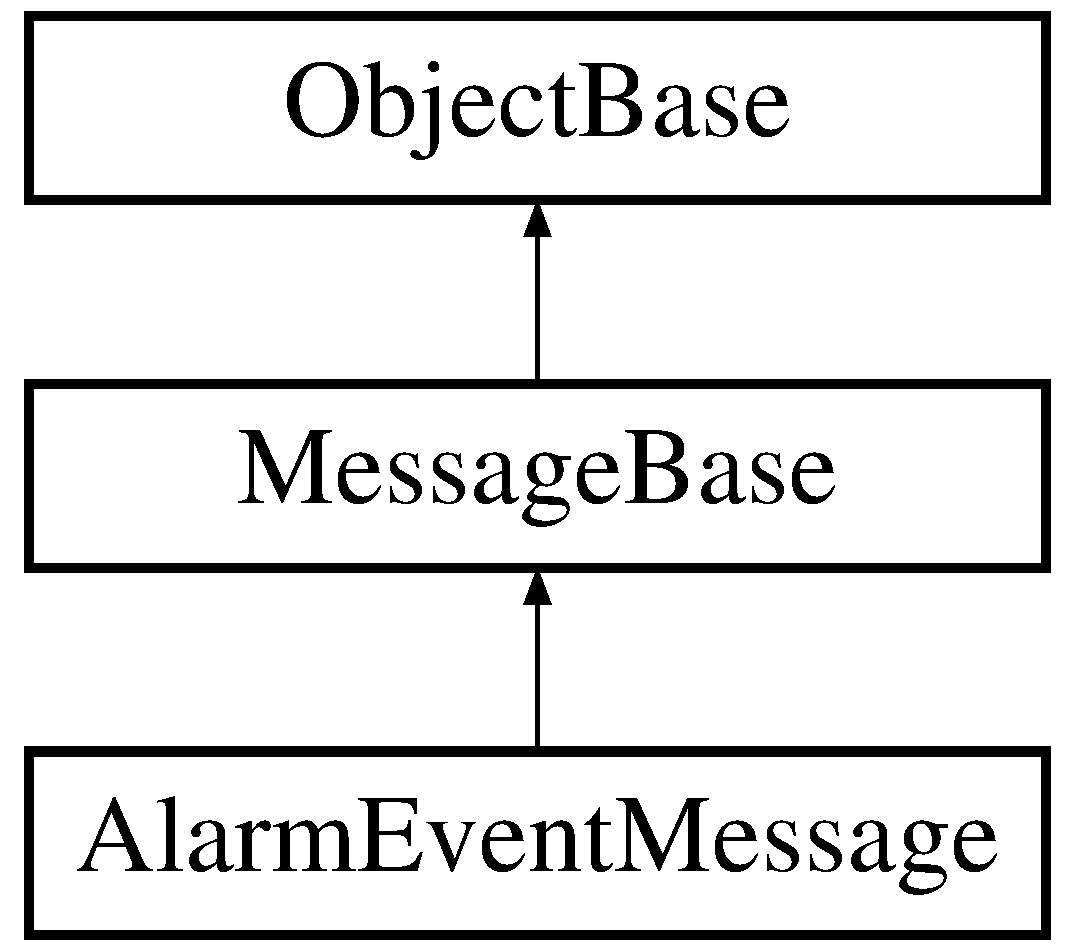
\includegraphics[height=3.000000cm]{classAlarmEventMessage}
\end{center}
\end{figure}
\subsection*{Public Member Functions}
\begin{DoxyCompactItemize}
\item 
{\bf Alarm\+Event\+Message} (const {\bf Mailbox\+Address} \&source\+Address, Alarm\+Event\+Message\+Type message\+Type, string neid, unsigned short managed\+Object, unsigned int managed\+Object\+Instance, unsigned short alarm\+Code, unsigned short event\+Code, unsigned int pid, unsigned int time\+Stamp, unsigned int source\+Context\+Id=0, unsigned int destination\+Context\+Id=0)
\item 
virtual {\bf $\sim$\+Alarm\+Event\+Message} ()
\item 
Alarm\+Event\+Message\+Type {\bf get\+Message\+Type} () const 
\item 
unsigned short {\bf get\+Message\+Id} () const 
\item 
string {\bf get\+N\+E\+ID} () const 
\item 
unsigned short {\bf get\+Managed\+Object} () const 
\item 
unsigned int {\bf get\+Managed\+Object\+Instance} () const 
\item 
unsigned short {\bf get\+Alarm\+Code} () const 
\item 
unsigned short {\bf get\+Event\+Code} () const 
\item 
unsigned int {\bf get\+Pid} () const 
\item 
unsigned int {\bf get\+Timestamp} () const 
\item 
int {\bf serialize} ({\bf Message\+Buffer} \&buffer)
\item 
string {\bf to\+String} ()
\end{DoxyCompactItemize}
\subsection*{Static Public Member Functions}
\begin{DoxyCompactItemize}
\item 
static {\bf Message\+Base} $\ast$ {\bf deserialize} ({\bf Message\+Buffer} $\ast$buffer)
\end{DoxyCompactItemize}
\subsection*{Additional Inherited Members}


\subsection{Constructor \& Destructor Documentation}
\index{Alarm\+Event\+Message@{Alarm\+Event\+Message}!Alarm\+Event\+Message@{Alarm\+Event\+Message}}
\index{Alarm\+Event\+Message@{Alarm\+Event\+Message}!Alarm\+Event\+Message@{Alarm\+Event\+Message}}
\subsubsection[{Alarm\+Event\+Message(const Mailbox\+Address \&source\+Address, Alarm\+Event\+Message\+Type message\+Type, string neid, unsigned short managed\+Object, unsigned int managed\+Object\+Instance, unsigned short alarm\+Code, unsigned short event\+Code, unsigned int pid, unsigned int time\+Stamp, unsigned int source\+Context\+Id=0, unsigned int destination\+Context\+Id=0)}]{\setlength{\rightskip}{0pt plus 5cm}Alarm\+Event\+Message\+::\+Alarm\+Event\+Message (
\begin{DoxyParamCaption}
\item[{const {\bf Mailbox\+Address} \&}]{source\+Address, }
\item[{Alarm\+Event\+Message\+Type}]{message\+Type, }
\item[{string}]{neid, }
\item[{unsigned short}]{managed\+Object, }
\item[{unsigned int}]{managed\+Object\+Instance, }
\item[{unsigned short}]{alarm\+Code, }
\item[{unsigned short}]{event\+Code, }
\item[{unsigned int}]{pid, }
\item[{unsigned int}]{time\+Stamp, }
\item[{unsigned int}]{source\+Context\+Id = {\ttfamily 0}, }
\item[{unsigned int}]{destination\+Context\+Id = {\ttfamily 0}}
\end{DoxyParamCaption}
)}\label{classAlarmEventMessage_a6ff212a826041ed2136b618b99e361f8}
Constructor 

Referenced by deserialize().

\index{Alarm\+Event\+Message@{Alarm\+Event\+Message}!````~Alarm\+Event\+Message@{$\sim$\+Alarm\+Event\+Message}}
\index{````~Alarm\+Event\+Message@{$\sim$\+Alarm\+Event\+Message}!Alarm\+Event\+Message@{Alarm\+Event\+Message}}
\subsubsection[{$\sim$\+Alarm\+Event\+Message()}]{\setlength{\rightskip}{0pt plus 5cm}Alarm\+Event\+Message\+::$\sim$\+Alarm\+Event\+Message (
\begin{DoxyParamCaption}
{}
\end{DoxyParamCaption}
)\hspace{0.3cm}{\ttfamily [virtual]}}\label{classAlarmEventMessage_aa047e19c515a18ef823595012a8854f8}
Virtual Destructor 

\subsection{Member Function Documentation}
\index{Alarm\+Event\+Message@{Alarm\+Event\+Message}!deserialize@{deserialize}}
\index{deserialize@{deserialize}!Alarm\+Event\+Message@{Alarm\+Event\+Message}}
\subsubsection[{deserialize(\+Message\+Buffer $\ast$buffer)}]{\setlength{\rightskip}{0pt plus 5cm}{\bf Message\+Base} $\ast$ Alarm\+Event\+Message\+::deserialize (
\begin{DoxyParamCaption}
\item[{{\bf Message\+Buffer} $\ast$}]{buffer}
\end{DoxyParamCaption}
)\hspace{0.3cm}{\ttfamily [static]}}\label{classAlarmEventMessage_aa44dd64923412b43074d8c55de6d494a}
Subclassed deserialization / bootstrap implementation 

References Alarm\+Event\+Message().

\index{Alarm\+Event\+Message@{Alarm\+Event\+Message}!get\+Alarm\+Code@{get\+Alarm\+Code}}
\index{get\+Alarm\+Code@{get\+Alarm\+Code}!Alarm\+Event\+Message@{Alarm\+Event\+Message}}
\subsubsection[{get\+Alarm\+Code() const }]{\setlength{\rightskip}{0pt plus 5cm}unsigned short Alarm\+Event\+Message\+::get\+Alarm\+Code (
\begin{DoxyParamCaption}
{}
\end{DoxyParamCaption}
) const}\label{classAlarmEventMessage_a8de85f019fdb8ea34b22736ae38df098}
Returns the alarm code \index{Alarm\+Event\+Message@{Alarm\+Event\+Message}!get\+Event\+Code@{get\+Event\+Code}}
\index{get\+Event\+Code@{get\+Event\+Code}!Alarm\+Event\+Message@{Alarm\+Event\+Message}}
\subsubsection[{get\+Event\+Code() const }]{\setlength{\rightskip}{0pt plus 5cm}unsigned short Alarm\+Event\+Message\+::get\+Event\+Code (
\begin{DoxyParamCaption}
{}
\end{DoxyParamCaption}
) const}\label{classAlarmEventMessage_adced09f552703d4b8f3ecfee2d835541}
Returns the event code \index{Alarm\+Event\+Message@{Alarm\+Event\+Message}!get\+Managed\+Object@{get\+Managed\+Object}}
\index{get\+Managed\+Object@{get\+Managed\+Object}!Alarm\+Event\+Message@{Alarm\+Event\+Message}}
\subsubsection[{get\+Managed\+Object() const }]{\setlength{\rightskip}{0pt plus 5cm}unsigned short Alarm\+Event\+Message\+::get\+Managed\+Object (
\begin{DoxyParamCaption}
{}
\end{DoxyParamCaption}
) const}\label{classAlarmEventMessage_a8938ad6884c3e0d4631e76ed3c13f6ca}
Returns the managed object class \index{Alarm\+Event\+Message@{Alarm\+Event\+Message}!get\+Managed\+Object\+Instance@{get\+Managed\+Object\+Instance}}
\index{get\+Managed\+Object\+Instance@{get\+Managed\+Object\+Instance}!Alarm\+Event\+Message@{Alarm\+Event\+Message}}
\subsubsection[{get\+Managed\+Object\+Instance() const }]{\setlength{\rightskip}{0pt plus 5cm}unsigned int Alarm\+Event\+Message\+::get\+Managed\+Object\+Instance (
\begin{DoxyParamCaption}
{}
\end{DoxyParamCaption}
) const}\label{classAlarmEventMessage_acff215e21f4c41b51b0ed7be357e5390}
Returns the managed object instance \index{Alarm\+Event\+Message@{Alarm\+Event\+Message}!get\+Message\+Id@{get\+Message\+Id}}
\index{get\+Message\+Id@{get\+Message\+Id}!Alarm\+Event\+Message@{Alarm\+Event\+Message}}
\subsubsection[{get\+Message\+Id() const }]{\setlength{\rightskip}{0pt plus 5cm}unsigned short Alarm\+Event\+Message\+::get\+Message\+Id (
\begin{DoxyParamCaption}
{}
\end{DoxyParamCaption}
) const\hspace{0.3cm}{\ttfamily [virtual]}}\label{classAlarmEventMessage_a9077b4f17fc3b57df685b1d3f34fdd91}
Returns the Message Id 

Implements {\bf Message\+Base} \doxyref{}{p.}{classMessageBase_a0910c23e94ea98b7a4e11631c9068311}.

\index{Alarm\+Event\+Message@{Alarm\+Event\+Message}!get\+Message\+Type@{get\+Message\+Type}}
\index{get\+Message\+Type@{get\+Message\+Type}!Alarm\+Event\+Message@{Alarm\+Event\+Message}}
\subsubsection[{get\+Message\+Type() const }]{\setlength{\rightskip}{0pt plus 5cm}Alarm\+Event\+Message\+Type Alarm\+Event\+Message\+::get\+Message\+Type (
\begin{DoxyParamCaption}
{}
\end{DoxyParamCaption}
) const}\label{classAlarmEventMessage_a56c63848af227441bc9304b7cb46036a}
Returns the Message Type (Alarm, Clear, Event\+Report) \index{Alarm\+Event\+Message@{Alarm\+Event\+Message}!get\+N\+E\+ID@{get\+N\+E\+ID}}
\index{get\+N\+E\+ID@{get\+N\+E\+ID}!Alarm\+Event\+Message@{Alarm\+Event\+Message}}
\subsubsection[{get\+N\+E\+I\+D() const }]{\setlength{\rightskip}{0pt plus 5cm}string Alarm\+Event\+Message\+::get\+N\+E\+ID (
\begin{DoxyParamCaption}
{}
\end{DoxyParamCaption}
) const}\label{classAlarmEventMessage_ae9b676a4004ec2d8c9c2ad9e6bff6ea7}
Returns the N\+E\+ID that the alarm applies to \index{Alarm\+Event\+Message@{Alarm\+Event\+Message}!get\+Pid@{get\+Pid}}
\index{get\+Pid@{get\+Pid}!Alarm\+Event\+Message@{Alarm\+Event\+Message}}
\subsubsection[{get\+Pid() const }]{\setlength{\rightskip}{0pt plus 5cm}unsigned int Alarm\+Event\+Message\+::get\+Pid (
\begin{DoxyParamCaption}
{}
\end{DoxyParamCaption}
) const}\label{classAlarmEventMessage_ad09b9844a8b5d47461ee224b1e846611}
Returns the process id \index{Alarm\+Event\+Message@{Alarm\+Event\+Message}!get\+Timestamp@{get\+Timestamp}}
\index{get\+Timestamp@{get\+Timestamp}!Alarm\+Event\+Message@{Alarm\+Event\+Message}}
\subsubsection[{get\+Timestamp() const }]{\setlength{\rightskip}{0pt plus 5cm}unsigned int Alarm\+Event\+Message\+::get\+Timestamp (
\begin{DoxyParamCaption}
{}
\end{DoxyParamCaption}
) const}\label{classAlarmEventMessage_ab4706d739eec6665f27525c169730ab0}
Returns the timestamp \index{Alarm\+Event\+Message@{Alarm\+Event\+Message}!serialize@{serialize}}
\index{serialize@{serialize}!Alarm\+Event\+Message@{Alarm\+Event\+Message}}
\subsubsection[{serialize(\+Message\+Buffer \&buffer)}]{\setlength{\rightskip}{0pt plus 5cm}int Alarm\+Event\+Message\+::serialize (
\begin{DoxyParamCaption}
\item[{{\bf Message\+Buffer} \&}]{buffer}
\end{DoxyParamCaption}
)\hspace{0.3cm}{\ttfamily [virtual]}}\label{classAlarmEventMessage_ac8f81237779034f177b908776029919c}
Subclassed serialization implementation 

Reimplemented from {\bf Message\+Base} \doxyref{}{p.}{classMessageBase_a1120deb2887e4a72d7dc68b505e5e10a}.



References Message\+Base\+::destination\+Context\+Id\+\_\+, Message\+Base\+::source\+Address\+\_\+, Message\+Base\+::source\+Context\+Id\+\_\+, and Message\+Base\+::version\+Number\+\_\+.

\index{Alarm\+Event\+Message@{Alarm\+Event\+Message}!to\+String@{to\+String}}
\index{to\+String@{to\+String}!Alarm\+Event\+Message@{Alarm\+Event\+Message}}
\subsubsection[{to\+String()}]{\setlength{\rightskip}{0pt plus 5cm}string Alarm\+Event\+Message\+::to\+String (
\begin{DoxyParamCaption}
{}
\end{DoxyParamCaption}
)\hspace{0.3cm}{\ttfamily [virtual]}}\label{classAlarmEventMessage_ad6d9f4689524920dac507f80424a5689}
String\textquotesingle{}ized debugging method \begin{DoxyReturn}{Returns}
string representation of the contents of this object 
\end{DoxyReturn}


Implements {\bf Message\+Base} \doxyref{}{p.}{classMessageBase_a7946fdcef86bfd67ad1df2ede8ed671d}.



References Message\+Base\+::source\+Address\+\_\+, and Mailbox\+Address\+::to\+String().



The documentation for this class was generated from the following files\+:\begin{DoxyCompactItemize}
\item 
Alarm\+Event\+Message.\+h\item 
Alarm\+Event\+Message.\+cpp\end{DoxyCompactItemize}

\section{C\+B\+Function\+Translator0$<$ Func $>$ Class Template Reference}
\label{classCBFunctionTranslator0}\index{C\+B\+Function\+Translator0$<$ Func $>$@{C\+B\+Function\+Translator0$<$ Func $>$}}
Inheritance diagram for C\+B\+Function\+Translator0$<$ Func $>$\+:\begin{figure}[H]
\begin{center}
\leavevmode
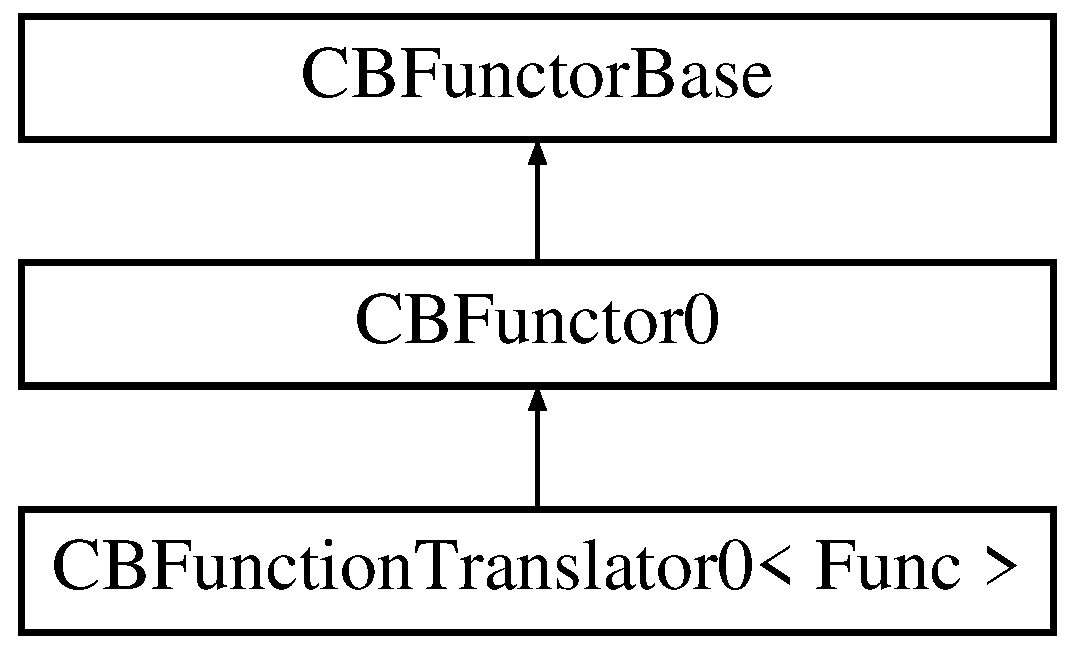
\includegraphics[height=3.000000cm]{classCBFunctionTranslator0}
\end{center}
\end{figure}
\subsection*{Public Member Functions}
\begin{DoxyCompactItemize}
\item 
{\bfseries C\+B\+Function\+Translator0} (Func f)\label{classCBFunctionTranslator0_a61103ab74629845b2d346a3f0920926f}

\end{DoxyCompactItemize}
\subsection*{Static Public Member Functions}
\begin{DoxyCompactItemize}
\item 
static void {\bfseries thunk} (const {\bf C\+B\+Functor\+Base} \&ftor)\label{classCBFunctionTranslator0_aeff9debdc4e6a3678d12e026b617612a}

\end{DoxyCompactItemize}
\subsection*{Additional Inherited Members}


The documentation for this class was generated from the following file\+:\begin{DoxyCompactItemize}
\item 
Callback.\+h\end{DoxyCompactItemize}

\section{C\+B\+Function\+Translator0w\+Ret$<$ RT, Func $>$ Class Template Reference}
\label{classCBFunctionTranslator0wRet}\index{C\+B\+Function\+Translator0w\+Ret$<$ R\+T, Func $>$@{C\+B\+Function\+Translator0w\+Ret$<$ R\+T, Func $>$}}
Inheritance diagram for C\+B\+Function\+Translator0w\+Ret$<$ RT, Func $>$\+:\begin{figure}[H]
\begin{center}
\leavevmode
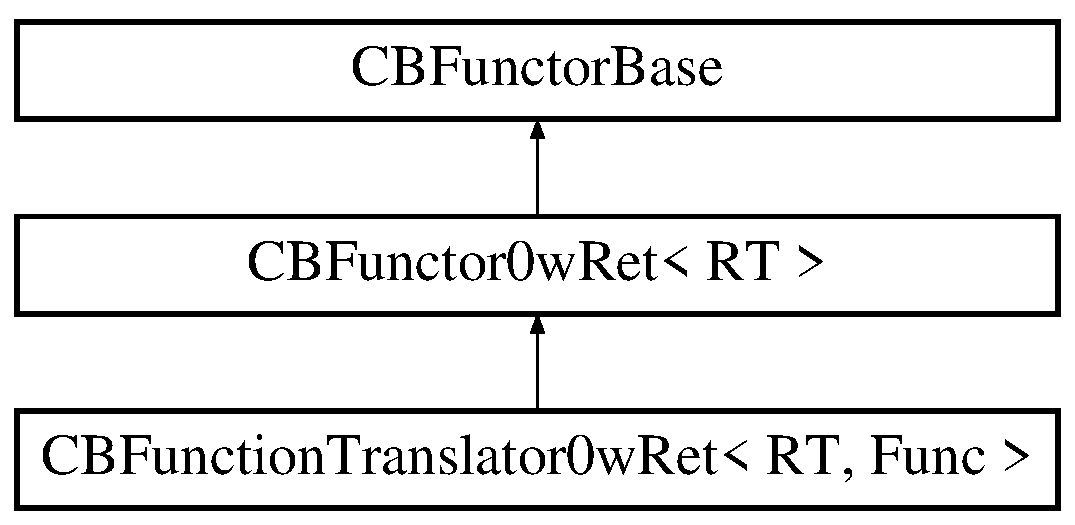
\includegraphics[height=3.000000cm]{classCBFunctionTranslator0wRet}
\end{center}
\end{figure}
\subsection*{Public Member Functions}
\begin{DoxyCompactItemize}
\item 
{\bfseries C\+B\+Function\+Translator0w\+Ret} (Func f)\label{classCBFunctionTranslator0wRet_a47476a9784c6b5ee86181c17c3846a5b}

\end{DoxyCompactItemize}
\subsection*{Static Public Member Functions}
\begin{DoxyCompactItemize}
\item 
static RT {\bfseries thunk} (const {\bf C\+B\+Functor\+Base} \&ftor)\label{classCBFunctionTranslator0wRet_a212480259869fd827e7159e6f986b909}

\end{DoxyCompactItemize}
\subsection*{Additional Inherited Members}


The documentation for this class was generated from the following file\+:\begin{DoxyCompactItemize}
\item 
Callback.\+h\end{DoxyCompactItemize}

\section{C\+B\+Function\+Translator1$<$ P1, Func $>$ Class Template Reference}
\label{classCBFunctionTranslator1}\index{C\+B\+Function\+Translator1$<$ P1, Func $>$@{C\+B\+Function\+Translator1$<$ P1, Func $>$}}
Inheritance diagram for C\+B\+Function\+Translator1$<$ P1, Func $>$\+:\begin{figure}[H]
\begin{center}
\leavevmode
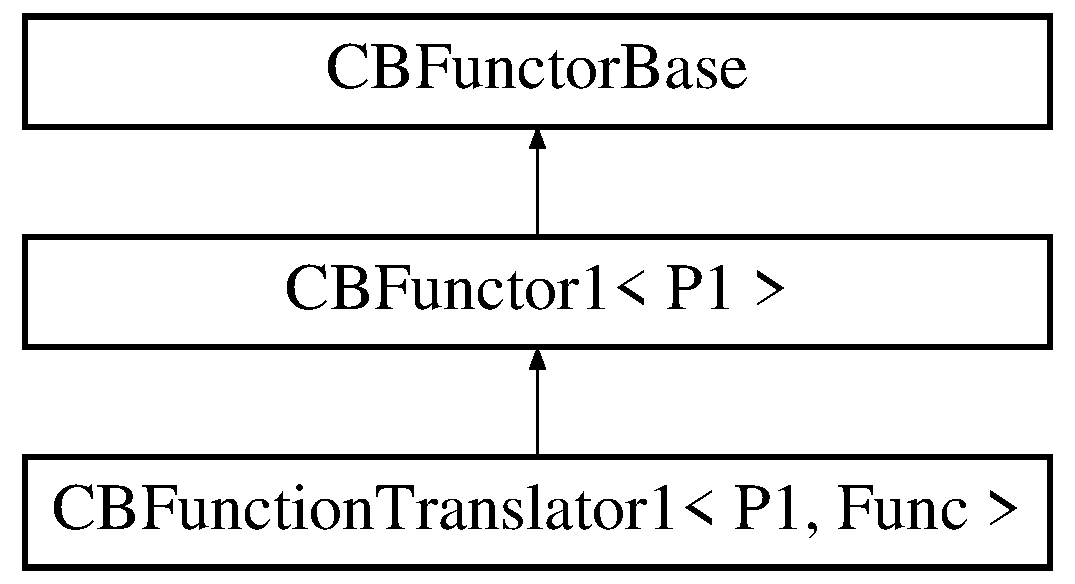
\includegraphics[height=3.000000cm]{classCBFunctionTranslator1}
\end{center}
\end{figure}
\subsection*{Public Member Functions}
\begin{DoxyCompactItemize}
\item 
{\bfseries C\+B\+Function\+Translator1} (Func f)\label{classCBFunctionTranslator1_ac72c06da799c65a37195218a5c800e12}

\end{DoxyCompactItemize}
\subsection*{Static Public Member Functions}
\begin{DoxyCompactItemize}
\item 
static void {\bfseries thunk} (const {\bf C\+B\+Functor\+Base} \&ftor, P1 p1)\label{classCBFunctionTranslator1_a7d85f4a12350666a798e1895afd5740c}

\end{DoxyCompactItemize}
\subsection*{Additional Inherited Members}


The documentation for this class was generated from the following file\+:\begin{DoxyCompactItemize}
\item 
Callback.\+h\end{DoxyCompactItemize}

\section{C\+B\+Function\+Translator1w\+Ret$<$ P1, RT, Func $>$ Class Template Reference}
\label{classCBFunctionTranslator1wRet}\index{C\+B\+Function\+Translator1w\+Ret$<$ P1, R\+T, Func $>$@{C\+B\+Function\+Translator1w\+Ret$<$ P1, R\+T, Func $>$}}
Inheritance diagram for C\+B\+Function\+Translator1w\+Ret$<$ P1, RT, Func $>$\+:\begin{figure}[H]
\begin{center}
\leavevmode
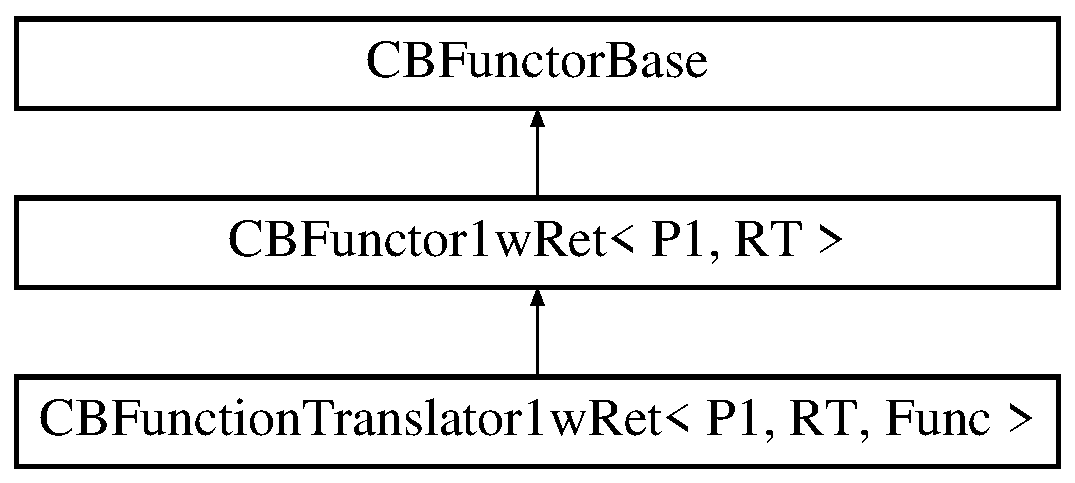
\includegraphics[height=3.000000cm]{classCBFunctionTranslator1wRet}
\end{center}
\end{figure}
\subsection*{Public Member Functions}
\begin{DoxyCompactItemize}
\item 
{\bfseries C\+B\+Function\+Translator1w\+Ret} (Func f)\label{classCBFunctionTranslator1wRet_aed1a0b2082a3dae5dfeaf467f2cf20dd}

\end{DoxyCompactItemize}
\subsection*{Static Public Member Functions}
\begin{DoxyCompactItemize}
\item 
static RT {\bfseries thunk} (const {\bf C\+B\+Functor\+Base} \&ftor, P1 p1)\label{classCBFunctionTranslator1wRet_a8a5d692b29dd3c76b1ea623c2e3c62a7}

\end{DoxyCompactItemize}
\subsection*{Additional Inherited Members}


The documentation for this class was generated from the following file\+:\begin{DoxyCompactItemize}
\item 
Callback.\+h\end{DoxyCompactItemize}

\section{C\+B\+Function\+Translator2$<$ P1, P2, Func $>$ Class Template Reference}
\label{classCBFunctionTranslator2}\index{C\+B\+Function\+Translator2$<$ P1, P2, Func $>$@{C\+B\+Function\+Translator2$<$ P1, P2, Func $>$}}
Inheritance diagram for C\+B\+Function\+Translator2$<$ P1, P2, Func $>$\+:\begin{figure}[H]
\begin{center}
\leavevmode
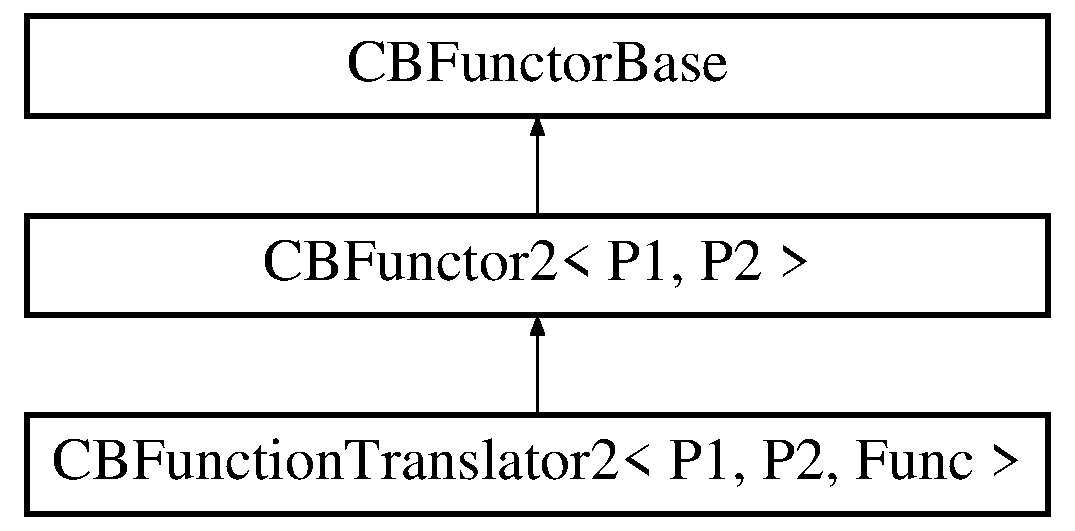
\includegraphics[height=3.000000cm]{classCBFunctionTranslator2}
\end{center}
\end{figure}
\subsection*{Public Member Functions}
\begin{DoxyCompactItemize}
\item 
{\bfseries C\+B\+Function\+Translator2} (Func f)\label{classCBFunctionTranslator2_a44ecf241306c6588d3498703101c08cb}

\end{DoxyCompactItemize}
\subsection*{Static Public Member Functions}
\begin{DoxyCompactItemize}
\item 
static void {\bfseries thunk} (const {\bf C\+B\+Functor\+Base} \&ftor, P1 p1, P2 p2)\label{classCBFunctionTranslator2_ac87f753ab63e1514c4d025b10dba2fc4}

\end{DoxyCompactItemize}
\subsection*{Additional Inherited Members}


The documentation for this class was generated from the following file\+:\begin{DoxyCompactItemize}
\item 
Callback.\+h\end{DoxyCompactItemize}

\section{C\+B\+Function\+Translator2w\+Ret$<$ P1, P2, RT, Func $>$ Class Template Reference}
\label{classCBFunctionTranslator2wRet}\index{C\+B\+Function\+Translator2w\+Ret$<$ P1, P2, R\+T, Func $>$@{C\+B\+Function\+Translator2w\+Ret$<$ P1, P2, R\+T, Func $>$}}
Inheritance diagram for C\+B\+Function\+Translator2w\+Ret$<$ P1, P2, RT, Func $>$\+:\begin{figure}[H]
\begin{center}
\leavevmode
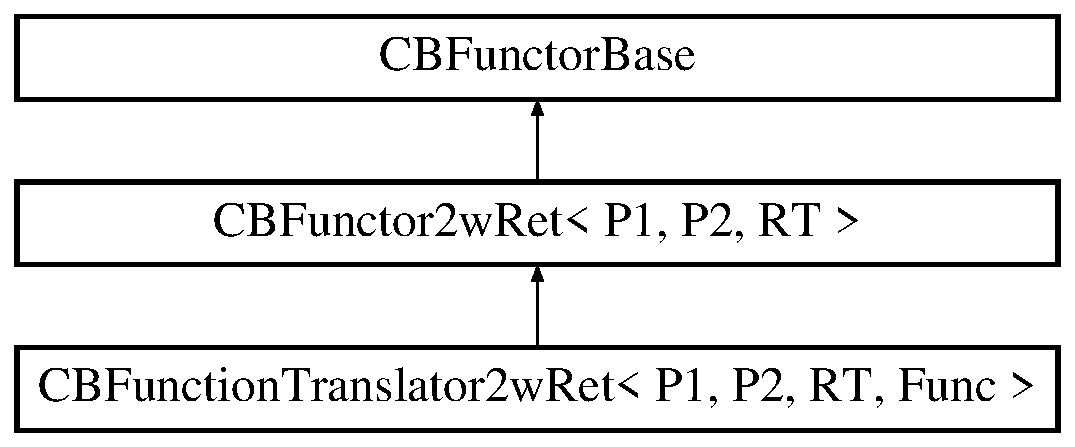
\includegraphics[height=3.000000cm]{classCBFunctionTranslator2wRet}
\end{center}
\end{figure}
\subsection*{Public Member Functions}
\begin{DoxyCompactItemize}
\item 
{\bfseries C\+B\+Function\+Translator2w\+Ret} (Func f)\label{classCBFunctionTranslator2wRet_ae3bc8f17074bb2229c7fcdff0ac43cd2}

\end{DoxyCompactItemize}
\subsection*{Static Public Member Functions}
\begin{DoxyCompactItemize}
\item 
static RT {\bfseries thunk} (const {\bf C\+B\+Functor\+Base} \&ftor, P1 p1, P2 p2)\label{classCBFunctionTranslator2wRet_adcb4d97648e50b15dd26f03646d20374}

\end{DoxyCompactItemize}
\subsection*{Additional Inherited Members}


The documentation for this class was generated from the following file\+:\begin{DoxyCompactItemize}
\item 
Callback.\+h\end{DoxyCompactItemize}

\section{C\+B\+Function\+Translator3$<$ P1, P2, P3, Func $>$ Class Template Reference}
\label{classCBFunctionTranslator3}\index{C\+B\+Function\+Translator3$<$ P1, P2, P3, Func $>$@{C\+B\+Function\+Translator3$<$ P1, P2, P3, Func $>$}}
Inheritance diagram for C\+B\+Function\+Translator3$<$ P1, P2, P3, Func $>$\+:\begin{figure}[H]
\begin{center}
\leavevmode
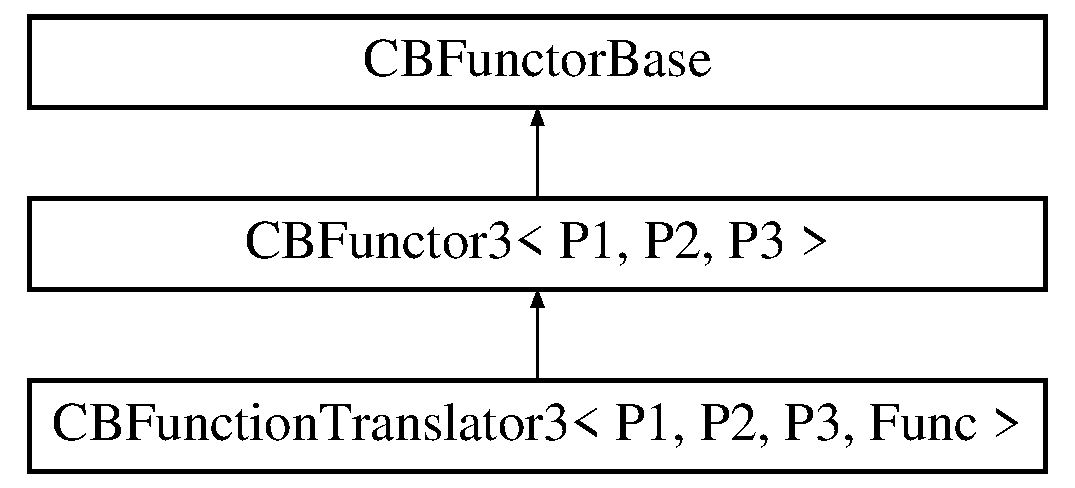
\includegraphics[height=3.000000cm]{classCBFunctionTranslator3}
\end{center}
\end{figure}
\subsection*{Public Member Functions}
\begin{DoxyCompactItemize}
\item 
{\bfseries C\+B\+Function\+Translator3} (Func f)\label{classCBFunctionTranslator3_a59d1209449916b44b8ff86c0101c2df8}

\end{DoxyCompactItemize}
\subsection*{Static Public Member Functions}
\begin{DoxyCompactItemize}
\item 
static void {\bfseries thunk} (const {\bf C\+B\+Functor\+Base} \&ftor, P1 p1, P2 p2, P3 p3)\label{classCBFunctionTranslator3_a5460798da25c1e51d51bdad9a8e79f57}

\end{DoxyCompactItemize}
\subsection*{Additional Inherited Members}


The documentation for this class was generated from the following file\+:\begin{DoxyCompactItemize}
\item 
Callback.\+h\end{DoxyCompactItemize}

\section{C\+B\+Function\+Translator3w\+Ret$<$ P1, P2, P3, RT, Func $>$ Class Template Reference}
\label{classCBFunctionTranslator3wRet}\index{C\+B\+Function\+Translator3w\+Ret$<$ P1, P2, P3, R\+T, Func $>$@{C\+B\+Function\+Translator3w\+Ret$<$ P1, P2, P3, R\+T, Func $>$}}
Inheritance diagram for C\+B\+Function\+Translator3w\+Ret$<$ P1, P2, P3, RT, Func $>$\+:\begin{figure}[H]
\begin{center}
\leavevmode
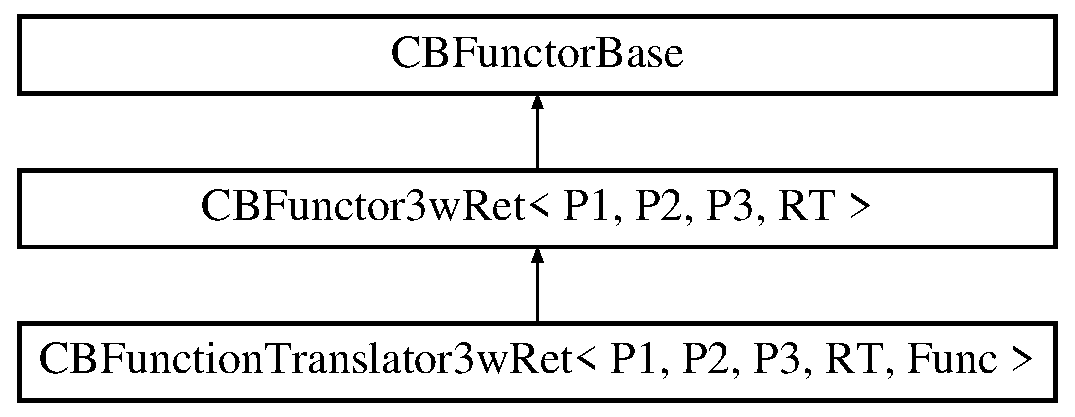
\includegraphics[height=3.000000cm]{classCBFunctionTranslator3wRet}
\end{center}
\end{figure}
\subsection*{Public Member Functions}
\begin{DoxyCompactItemize}
\item 
{\bfseries C\+B\+Function\+Translator3w\+Ret} (Func f)\label{classCBFunctionTranslator3wRet_ac2b6449f80ddab6b24af1d17bf7c7453}

\end{DoxyCompactItemize}
\subsection*{Static Public Member Functions}
\begin{DoxyCompactItemize}
\item 
static RT {\bfseries thunk} (const {\bf C\+B\+Functor\+Base} \&ftor, P1 p1, P2 p2, P3 p3)\label{classCBFunctionTranslator3wRet_a05ba9d1d3e8224bf08097b8dfe9f93cf}

\end{DoxyCompactItemize}
\subsection*{Additional Inherited Members}


The documentation for this class was generated from the following file\+:\begin{DoxyCompactItemize}
\item 
Callback.\+h\end{DoxyCompactItemize}

\section{C\+B\+Function\+Translator4$<$ P1, P2, P3, P4, Func $>$ Class Template Reference}
\label{classCBFunctionTranslator4}\index{C\+B\+Function\+Translator4$<$ P1, P2, P3, P4, Func $>$@{C\+B\+Function\+Translator4$<$ P1, P2, P3, P4, Func $>$}}
Inheritance diagram for C\+B\+Function\+Translator4$<$ P1, P2, P3, P4, Func $>$\+:\begin{figure}[H]
\begin{center}
\leavevmode
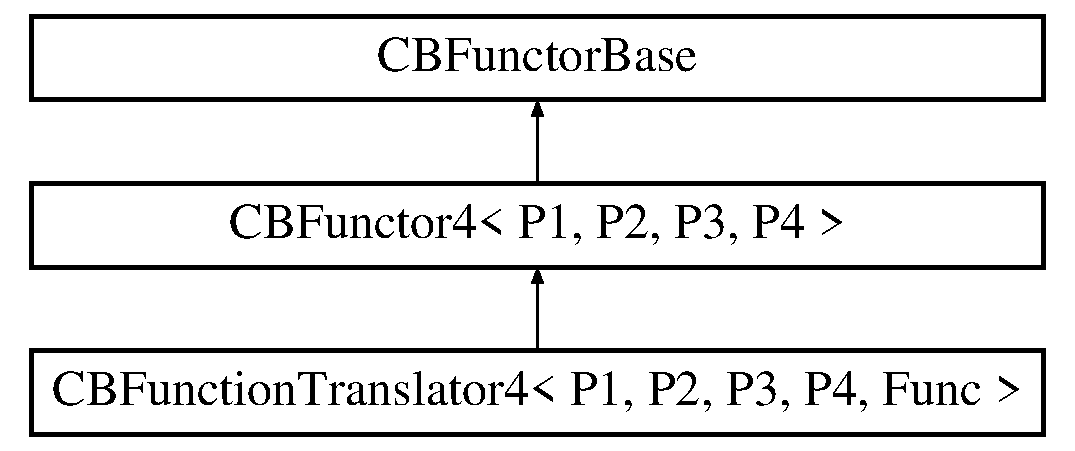
\includegraphics[height=3.000000cm]{classCBFunctionTranslator4}
\end{center}
\end{figure}
\subsection*{Public Member Functions}
\begin{DoxyCompactItemize}
\item 
{\bfseries C\+B\+Function\+Translator4} (Func f)\label{classCBFunctionTranslator4_ae810433e97712ca1cc6fc0f45d49dc31}

\end{DoxyCompactItemize}
\subsection*{Static Public Member Functions}
\begin{DoxyCompactItemize}
\item 
static void {\bfseries thunk} (const {\bf C\+B\+Functor\+Base} \&ftor, P1 p1, P2 p2, P3 p3, P4 p4)\label{classCBFunctionTranslator4_aca29fc798d6345156a1375d66713dc96}

\end{DoxyCompactItemize}
\subsection*{Additional Inherited Members}


The documentation for this class was generated from the following file\+:\begin{DoxyCompactItemize}
\item 
Callback.\+h\end{DoxyCompactItemize}

\section{C\+B\+Function\+Translator4w\+Ret$<$ P1, P2, P3, P4, RT, Func $>$ Class Template Reference}
\label{classCBFunctionTranslator4wRet}\index{C\+B\+Function\+Translator4w\+Ret$<$ P1, P2, P3, P4, R\+T, Func $>$@{C\+B\+Function\+Translator4w\+Ret$<$ P1, P2, P3, P4, R\+T, Func $>$}}
Inheritance diagram for C\+B\+Function\+Translator4w\+Ret$<$ P1, P2, P3, P4, RT, Func $>$\+:\begin{figure}[H]
\begin{center}
\leavevmode
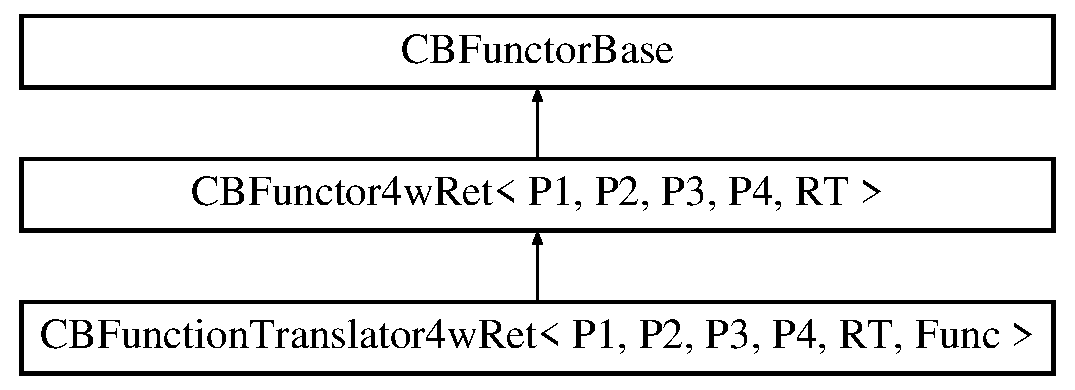
\includegraphics[height=3.000000cm]{classCBFunctionTranslator4wRet}
\end{center}
\end{figure}
\subsection*{Public Member Functions}
\begin{DoxyCompactItemize}
\item 
{\bfseries C\+B\+Function\+Translator4w\+Ret} (Func f)\label{classCBFunctionTranslator4wRet_a9af730c577866db61c9d85d1449f6fae}

\end{DoxyCompactItemize}
\subsection*{Static Public Member Functions}
\begin{DoxyCompactItemize}
\item 
static RT {\bfseries thunk} (const {\bf C\+B\+Functor\+Base} \&ftor, P1 p1, P2 p2, P3 p3, P4 p4)\label{classCBFunctionTranslator4wRet_a9f628525b525c0307d739c66f27bfd46}

\end{DoxyCompactItemize}
\subsection*{Additional Inherited Members}


The documentation for this class was generated from the following file\+:\begin{DoxyCompactItemize}
\item 
Callback.\+h\end{DoxyCompactItemize}

\section{C\+B\+Functor0 Class Reference}
\label{classCBFunctor0}\index{C\+B\+Functor0@{C\+B\+Functor0}}
Inheritance diagram for C\+B\+Functor0\+:\begin{figure}[H]
\begin{center}
\leavevmode
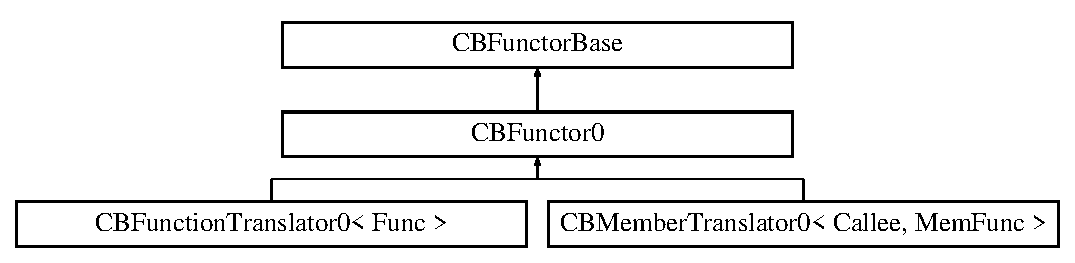
\includegraphics[height=3.000000cm]{classCBFunctor0}
\end{center}
\end{figure}
\subsection*{Public Member Functions}
\begin{DoxyCompactItemize}
\item 
{\bfseries C\+B\+Functor0} (R\+H\+C\+B\+\_\+\+D\+U\+M\+M\+Y\+\_\+\+I\+N\+IT=0)\label{classCBFunctor0_aa261471abb59323a151f573e50ab389c}

\item 
void {\bfseries operator()} () const \label{classCBFunctor0_a202aaeb45c6bfeaf12d2c41da3196a4c}

\end{DoxyCompactItemize}
\subsection*{Protected Types}
\begin{DoxyCompactItemize}
\item 
typedef void($\ast$ {\bfseries Thunk}) (const {\bf C\+B\+Functor\+Base} \&)\label{classCBFunctor0_a8cf13cb7f7b9e28615f907a8fed82156}

\end{DoxyCompactItemize}
\subsection*{Protected Member Functions}
\begin{DoxyCompactItemize}
\item 
{\bfseries C\+B\+Functor0} (Thunk t, const void $\ast$c, P\+Func f, const void $\ast$mf, size\+\_\+t sz)\label{classCBFunctor0_af657992d8a4b03d924f9158f6736efd4}

\end{DoxyCompactItemize}
\subsection*{Additional Inherited Members}


The documentation for this class was generated from the following file\+:\begin{DoxyCompactItemize}
\item 
Callback.\+h\end{DoxyCompactItemize}

\section{C\+B\+Functor0w\+Ret$<$ RT $>$ Class Template Reference}
\label{classCBFunctor0wRet}\index{C\+B\+Functor0w\+Ret$<$ R\+T $>$@{C\+B\+Functor0w\+Ret$<$ R\+T $>$}}
Inheritance diagram for C\+B\+Functor0w\+Ret$<$ RT $>$\+:\begin{figure}[H]
\begin{center}
\leavevmode
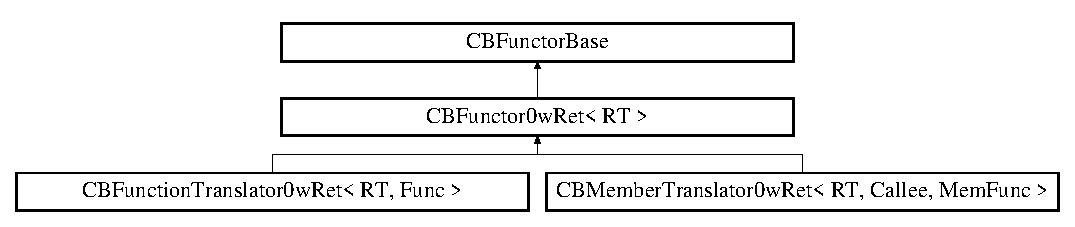
\includegraphics[height=2.600619cm]{classCBFunctor0wRet}
\end{center}
\end{figure}
\subsection*{Public Member Functions}
\begin{DoxyCompactItemize}
\item 
{\bfseries C\+B\+Functor0w\+Ret} (R\+H\+C\+B\+\_\+\+D\+U\+M\+M\+Y\+\_\+\+I\+N\+IT=0)\label{classCBFunctor0wRet_a3011430b893c45ff3ab2fa57914c5ab7}

\item 
RT {\bfseries operator()} () const \label{classCBFunctor0wRet_af1ef6bed1d39de94804f28ed204a1fb4}

\end{DoxyCompactItemize}
\subsection*{Protected Types}
\begin{DoxyCompactItemize}
\item 
typedef RT($\ast$ {\bfseries Thunk}) (const {\bf C\+B\+Functor\+Base} \&)\label{classCBFunctor0wRet_ac692081fb628516cfe434239ee222721}

\end{DoxyCompactItemize}
\subsection*{Protected Member Functions}
\begin{DoxyCompactItemize}
\item 
{\bfseries C\+B\+Functor0w\+Ret} (Thunk t, const void $\ast$c, P\+Func f, const void $\ast$mf, size\+\_\+t sz)\label{classCBFunctor0wRet_a033b2bd9af030ea5e54f35f0e1557459}

\end{DoxyCompactItemize}
\subsection*{Additional Inherited Members}


The documentation for this class was generated from the following file\+:\begin{DoxyCompactItemize}
\item 
Callback.\+h\end{DoxyCompactItemize}

\section{C\+B\+Functor1$<$ P1 $>$ Class Template Reference}
\label{classCBFunctor1}\index{C\+B\+Functor1$<$ P1 $>$@{C\+B\+Functor1$<$ P1 $>$}}
Inheritance diagram for C\+B\+Functor1$<$ P1 $>$\+:\begin{figure}[H]
\begin{center}
\leavevmode
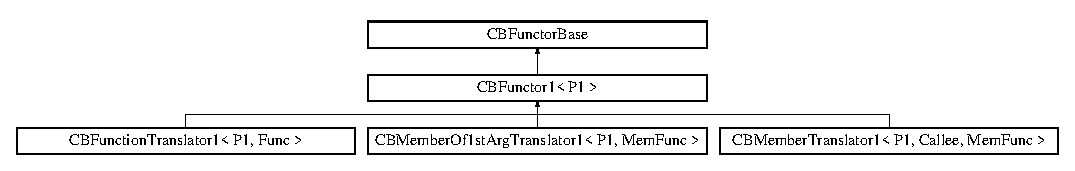
\includegraphics[height=1.854305cm]{classCBFunctor1}
\end{center}
\end{figure}
\subsection*{Public Types}
\begin{DoxyCompactItemize}
\item 
typedef P1 {\bfseries argument\+\_\+type}\label{classCBFunctor1_ad53b976c17b95b8170f3597725821386}

\item 
typedef void {\bfseries result\+\_\+type}\label{classCBFunctor1_a6803f5dfe59d2edeb3988b09b7d73b6e}

\end{DoxyCompactItemize}
\subsection*{Public Member Functions}
\begin{DoxyCompactItemize}
\item 
{\bfseries C\+B\+Functor1} (R\+H\+C\+B\+\_\+\+D\+U\+M\+M\+Y\+\_\+\+I\+N\+IT=0)\label{classCBFunctor1_a732275eb7e272ade6a20cf4d973ac7e0}

\item 
void {\bfseries operator()} (P1 p1) const \label{classCBFunctor1_a0d9c9376cf5017cc26c96e7cb66adda1}

\end{DoxyCompactItemize}
\subsection*{Protected Types}
\begin{DoxyCompactItemize}
\item 
typedef void($\ast$ {\bfseries Thunk}) (const {\bf C\+B\+Functor\+Base} \&, P1)\label{classCBFunctor1_a5c35fac68dfbf3be1b9af6d23504d6f9}

\end{DoxyCompactItemize}
\subsection*{Protected Member Functions}
\begin{DoxyCompactItemize}
\item 
{\bfseries C\+B\+Functor1} (Thunk t, const void $\ast$c, P\+Func f, const void $\ast$mf, size\+\_\+t sz)\label{classCBFunctor1_ab244cc7ecd861d72918ae3e02694b1c1}

\end{DoxyCompactItemize}
\subsection*{Additional Inherited Members}


The documentation for this class was generated from the following file\+:\begin{DoxyCompactItemize}
\item 
Callback.\+h\end{DoxyCompactItemize}

\section{C\+B\+Functor1w\+Ret$<$ P1, RT $>$ Class Template Reference}
\label{classCBFunctor1wRet}\index{C\+B\+Functor1w\+Ret$<$ P1, R\+T $>$@{C\+B\+Functor1w\+Ret$<$ P1, R\+T $>$}}
Inheritance diagram for C\+B\+Functor1w\+Ret$<$ P1, RT $>$\+:\begin{figure}[H]
\begin{center}
\leavevmode
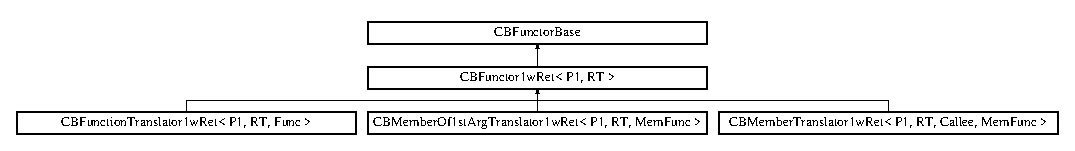
\includegraphics[height=1.586402cm]{classCBFunctor1wRet}
\end{center}
\end{figure}
\subsection*{Public Types}
\begin{DoxyCompactItemize}
\item 
typedef P1 {\bfseries argument\+\_\+type}\label{classCBFunctor1wRet_a3b06b725cdb955ad2300fd32c18fabd0}

\item 
typedef RT {\bfseries result\+\_\+type}\label{classCBFunctor1wRet_aedd72816facfbae9a1dc7908b7f9eeef}

\end{DoxyCompactItemize}
\subsection*{Public Member Functions}
\begin{DoxyCompactItemize}
\item 
{\bfseries C\+B\+Functor1w\+Ret} (R\+H\+C\+B\+\_\+\+D\+U\+M\+M\+Y\+\_\+\+I\+N\+IT=0)\label{classCBFunctor1wRet_ae617d4cc3513b4d18de4fb38857b6c2c}

\item 
RT {\bfseries operator()} (P1 p1) const \label{classCBFunctor1wRet_afd89568c8af023ef3f509cd7e1e444a9}

\end{DoxyCompactItemize}
\subsection*{Protected Types}
\begin{DoxyCompactItemize}
\item 
typedef RT($\ast$ {\bfseries Thunk}) (const {\bf C\+B\+Functor\+Base} \&, P1)\label{classCBFunctor1wRet_ac3c4c79ce83a99130c7d46acd4b8b681}

\end{DoxyCompactItemize}
\subsection*{Protected Member Functions}
\begin{DoxyCompactItemize}
\item 
{\bfseries C\+B\+Functor1w\+Ret} (Thunk t, const void $\ast$c, P\+Func f, const void $\ast$mf, size\+\_\+t sz)\label{classCBFunctor1wRet_a16b528d689792b58a510a5e7fff23e7c}

\end{DoxyCompactItemize}
\subsection*{Additional Inherited Members}


The documentation for this class was generated from the following file\+:\begin{DoxyCompactItemize}
\item 
Callback.\+h\end{DoxyCompactItemize}

\section{C\+B\+Functor2$<$ P1, P2 $>$ Class Template Reference}
\label{classCBFunctor2}\index{C\+B\+Functor2$<$ P1, P2 $>$@{C\+B\+Functor2$<$ P1, P2 $>$}}
Inheritance diagram for C\+B\+Functor2$<$ P1, P2 $>$\+:\begin{figure}[H]
\begin{center}
\leavevmode
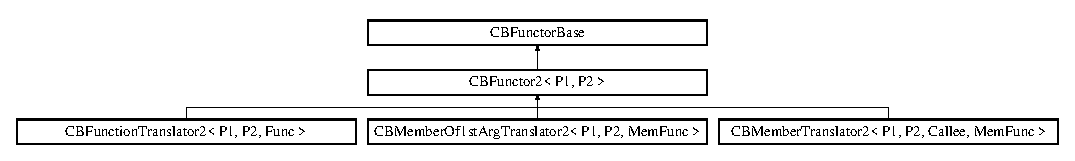
\includegraphics[height=1.717791cm]{classCBFunctor2}
\end{center}
\end{figure}
\subsection*{Public Types}
\begin{DoxyCompactItemize}
\item 
typedef P1 {\bfseries first\+\_\+argument\+\_\+type}\label{classCBFunctor2_a0b602135cc723557db0a98baac332f64}

\item 
typedef P2 {\bfseries second\+\_\+argument\+\_\+type}\label{classCBFunctor2_a42cb017aa79a85ae6c4c0d908b40b6e4}

\item 
typedef void {\bfseries result\+\_\+type}\label{classCBFunctor2_a7043f721c3f7cc64589a88ba678ade59}

\end{DoxyCompactItemize}
\subsection*{Public Member Functions}
\begin{DoxyCompactItemize}
\item 
{\bfseries C\+B\+Functor2} (R\+H\+C\+B\+\_\+\+D\+U\+M\+M\+Y\+\_\+\+I\+N\+IT=0)\label{classCBFunctor2_ab60622cec9febd42e7916f92567bc223}

\item 
void {\bfseries operator()} (P1 p1, P2 p2) const \label{classCBFunctor2_a8ef9e7a58474f11df3e9b0db59068016}

\end{DoxyCompactItemize}
\subsection*{Protected Types}
\begin{DoxyCompactItemize}
\item 
typedef void($\ast$ {\bfseries Thunk}) (const {\bf C\+B\+Functor\+Base} \&, P1, P2)\label{classCBFunctor2_a635d8110a9fae90fb52977641b980241}

\end{DoxyCompactItemize}
\subsection*{Protected Member Functions}
\begin{DoxyCompactItemize}
\item 
{\bfseries C\+B\+Functor2} (Thunk t, const void $\ast$c, P\+Func f, const void $\ast$mf, size\+\_\+t sz)\label{classCBFunctor2_a29ed0870454c88ea38a030f4c1f341d1}

\end{DoxyCompactItemize}
\subsection*{Additional Inherited Members}


The documentation for this class was generated from the following file\+:\begin{DoxyCompactItemize}
\item 
Callback.\+h\end{DoxyCompactItemize}

\section{C\+B\+Functor2w\+Ret$<$ P1, P2, RT $>$ Class Template Reference}
\label{classCBFunctor2wRet}\index{C\+B\+Functor2w\+Ret$<$ P1, P2, R\+T $>$@{C\+B\+Functor2w\+Ret$<$ P1, P2, R\+T $>$}}
Inheritance diagram for C\+B\+Functor2w\+Ret$<$ P1, P2, RT $>$\+:\begin{figure}[H]
\begin{center}
\leavevmode
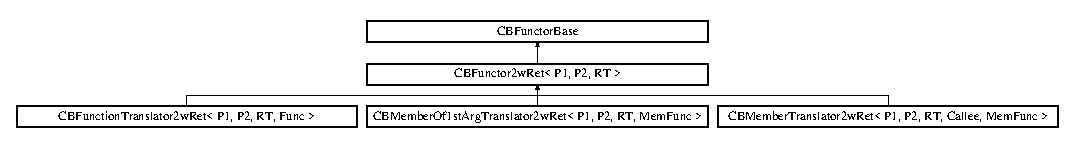
\includegraphics[height=1.485411cm]{classCBFunctor2wRet}
\end{center}
\end{figure}
\subsection*{Public Types}
\begin{DoxyCompactItemize}
\item 
typedef P1 {\bfseries first\+\_\+argument\+\_\+type}\label{classCBFunctor2wRet_a7d24bfcc6aa65aa4b55b5e959a004dd4}

\item 
typedef P2 {\bfseries second\+\_\+argument\+\_\+type}\label{classCBFunctor2wRet_ab581d0954897537b10bf2de447b8b657}

\item 
typedef RT {\bfseries result\+\_\+type}\label{classCBFunctor2wRet_a9d2ef5e7ee4eaac99bea7abfdd21af82}

\end{DoxyCompactItemize}
\subsection*{Public Member Functions}
\begin{DoxyCompactItemize}
\item 
{\bfseries C\+B\+Functor2w\+Ret} (R\+H\+C\+B\+\_\+\+D\+U\+M\+M\+Y\+\_\+\+I\+N\+IT=0)\label{classCBFunctor2wRet_a72315832a0fbc1a017d94c6d1a0744ea}

\item 
RT {\bfseries operator()} (P1 p1, P2 p2) const \label{classCBFunctor2wRet_ac6c5aa2cc0ec49461fef4031c2550121}

\end{DoxyCompactItemize}
\subsection*{Protected Types}
\begin{DoxyCompactItemize}
\item 
typedef RT($\ast$ {\bfseries Thunk}) (const {\bf C\+B\+Functor\+Base} \&, P1, P2)\label{classCBFunctor2wRet_ae2a1a21268a5beaac9acd0f08bcaee29}

\end{DoxyCompactItemize}
\subsection*{Protected Member Functions}
\begin{DoxyCompactItemize}
\item 
{\bfseries C\+B\+Functor2w\+Ret} (Thunk t, const void $\ast$c, P\+Func f, const void $\ast$mf, size\+\_\+t sz)\label{classCBFunctor2wRet_a8048bc4a33945fc5f5bbee22097fcafa}

\end{DoxyCompactItemize}
\subsection*{Additional Inherited Members}


The documentation for this class was generated from the following file\+:\begin{DoxyCompactItemize}
\item 
Callback.\+h\end{DoxyCompactItemize}

\section{C\+B\+Functor3$<$ P1, P2, P3 $>$ Class Template Reference}
\label{classCBFunctor3}\index{C\+B\+Functor3$<$ P1, P2, P3 $>$@{C\+B\+Functor3$<$ P1, P2, P3 $>$}}
Inheritance diagram for C\+B\+Functor3$<$ P1, P2, P3 $>$\+:\begin{figure}[H]
\begin{center}
\leavevmode
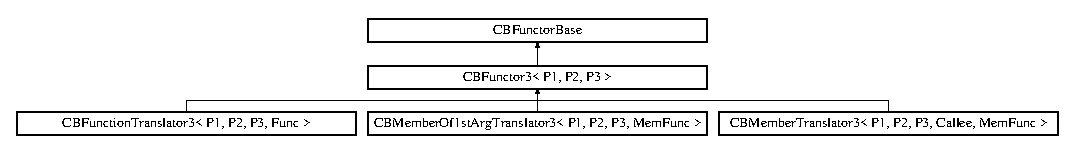
\includegraphics[height=1.600000cm]{classCBFunctor3}
\end{center}
\end{figure}
\subsection*{Public Member Functions}
\begin{DoxyCompactItemize}
\item 
{\bfseries C\+B\+Functor3} (R\+H\+C\+B\+\_\+\+D\+U\+M\+M\+Y\+\_\+\+I\+N\+IT=0)\label{classCBFunctor3_a45aabe3aa7d80c6d9b8fa5bec4d892f4}

\item 
void {\bfseries operator()} (P1 p1, P2 p2, P3 p3) const \label{classCBFunctor3_a716caade0cfc26f54604c2417fa0ce1f}

\end{DoxyCompactItemize}
\subsection*{Protected Types}
\begin{DoxyCompactItemize}
\item 
typedef void($\ast$ {\bfseries Thunk}) (const {\bf C\+B\+Functor\+Base} \&, P1, P2, P3)\label{classCBFunctor3_acfad242f124c1c40f0fbe769ec19a745}

\end{DoxyCompactItemize}
\subsection*{Protected Member Functions}
\begin{DoxyCompactItemize}
\item 
{\bfseries C\+B\+Functor3} (Thunk t, const void $\ast$c, P\+Func f, const void $\ast$mf, size\+\_\+t sz)\label{classCBFunctor3_a43d500e453926d91d935ff813bbfb7f2}

\end{DoxyCompactItemize}
\subsection*{Additional Inherited Members}


The documentation for this class was generated from the following file\+:\begin{DoxyCompactItemize}
\item 
Callback.\+h\end{DoxyCompactItemize}

\section{C\+B\+Functor3w\+Ret$<$ P1, P2, P3, RT $>$ Class Template Reference}
\label{classCBFunctor3wRet}\index{C\+B\+Functor3w\+Ret$<$ P1, P2, P3, R\+T $>$@{C\+B\+Functor3w\+Ret$<$ P1, P2, P3, R\+T $>$}}
Inheritance diagram for C\+B\+Functor3w\+Ret$<$ P1, P2, P3, RT $>$\+:\begin{figure}[H]
\begin{center}
\leavevmode
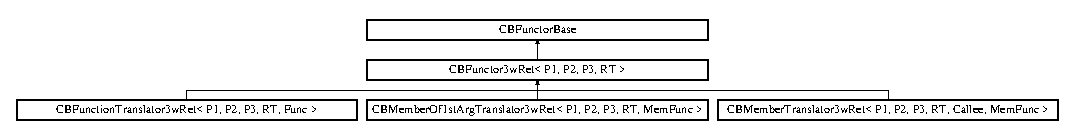
\includegraphics[height=1.396509cm]{classCBFunctor3wRet}
\end{center}
\end{figure}
\subsection*{Public Member Functions}
\begin{DoxyCompactItemize}
\item 
{\bfseries C\+B\+Functor3w\+Ret} (R\+H\+C\+B\+\_\+\+D\+U\+M\+M\+Y\+\_\+\+I\+N\+IT=0)\label{classCBFunctor3wRet_a55a3f8a8ee1c4cc3d287e0998560fce7}

\item 
RT {\bfseries operator()} (P1 p1, P2 p2, P3 p3) const \label{classCBFunctor3wRet_a00518cbfceca05d2f590658dff0a9120}

\end{DoxyCompactItemize}
\subsection*{Protected Types}
\begin{DoxyCompactItemize}
\item 
typedef RT($\ast$ {\bfseries Thunk}) (const {\bf C\+B\+Functor\+Base} \&, P1, P2, P3)\label{classCBFunctor3wRet_aca2bfd8d5602ca752219aeca7686e783}

\end{DoxyCompactItemize}
\subsection*{Protected Member Functions}
\begin{DoxyCompactItemize}
\item 
{\bfseries C\+B\+Functor3w\+Ret} (Thunk t, const void $\ast$c, P\+Func f, const void $\ast$mf, size\+\_\+t sz)\label{classCBFunctor3wRet_ab7b68e0f6a7dd2e53055a3c1405ee329}

\end{DoxyCompactItemize}
\subsection*{Additional Inherited Members}


The documentation for this class was generated from the following file\+:\begin{DoxyCompactItemize}
\item 
Callback.\+h\end{DoxyCompactItemize}

\section{C\+B\+Functor4$<$ P1, P2, P3, P4 $>$ Class Template Reference}
\label{classCBFunctor4}\index{C\+B\+Functor4$<$ P1, P2, P3, P4 $>$@{C\+B\+Functor4$<$ P1, P2, P3, P4 $>$}}
Inheritance diagram for C\+B\+Functor4$<$ P1, P2, P3, P4 $>$\+:\begin{figure}[H]
\begin{center}
\leavevmode
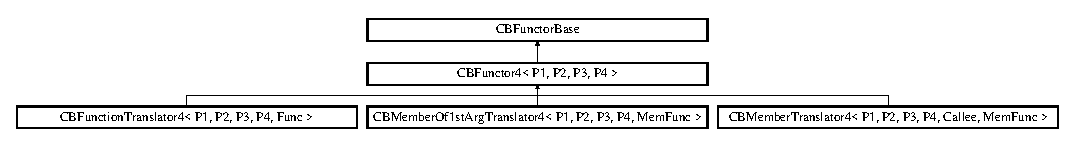
\includegraphics[height=1.497326cm]{classCBFunctor4}
\end{center}
\end{figure}
\subsection*{Public Member Functions}
\begin{DoxyCompactItemize}
\item 
{\bfseries C\+B\+Functor4} (R\+H\+C\+B\+\_\+\+D\+U\+M\+M\+Y\+\_\+\+I\+N\+IT=0)\label{classCBFunctor4_ab9f1fe157970957cfd384ee87df43e7d}

\item 
void {\bfseries operator()} (P1 p1, P2 p2, P3 p3, P4 p4) const \label{classCBFunctor4_a11b13f6aec932f356744e591b9bddb78}

\end{DoxyCompactItemize}
\subsection*{Protected Types}
\begin{DoxyCompactItemize}
\item 
typedef void($\ast$ {\bfseries Thunk}) (const {\bf C\+B\+Functor\+Base} \&, P1, P2, P3, P4)\label{classCBFunctor4_a39760d7f6823b11e09bfeb34944ff57d}

\end{DoxyCompactItemize}
\subsection*{Protected Member Functions}
\begin{DoxyCompactItemize}
\item 
{\bfseries C\+B\+Functor4} (Thunk t, const void $\ast$c, P\+Func f, const void $\ast$mf, size\+\_\+t sz)\label{classCBFunctor4_a93c1195373bbd68970b079681b4df68b}

\end{DoxyCompactItemize}
\subsection*{Additional Inherited Members}


The documentation for this class was generated from the following file\+:\begin{DoxyCompactItemize}
\item 
Callback.\+h\end{DoxyCompactItemize}

\section{C\+B\+Functor4w\+Ret$<$ P1, P2, P3, P4, RT $>$ Class Template Reference}
\label{classCBFunctor4wRet}\index{C\+B\+Functor4w\+Ret$<$ P1, P2, P3, P4, R\+T $>$@{C\+B\+Functor4w\+Ret$<$ P1, P2, P3, P4, R\+T $>$}}
Inheritance diagram for C\+B\+Functor4w\+Ret$<$ P1, P2, P3, P4, RT $>$\+:\begin{figure}[H]
\begin{center}
\leavevmode
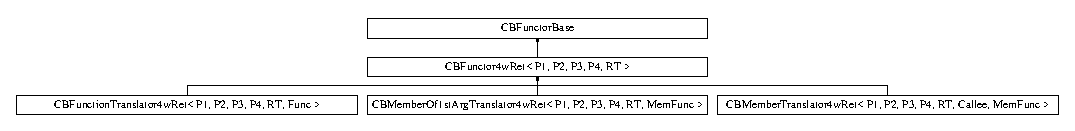
\includegraphics[height=1.317647cm]{classCBFunctor4wRet}
\end{center}
\end{figure}
\subsection*{Public Member Functions}
\begin{DoxyCompactItemize}
\item 
{\bfseries C\+B\+Functor4w\+Ret} (R\+H\+C\+B\+\_\+\+D\+U\+M\+M\+Y\+\_\+\+I\+N\+IT=0)\label{classCBFunctor4wRet_a36a036c2ab029c219d7e0f76f5c6888b}

\item 
RT {\bfseries operator()} (P1 p1, P2 p2, P3 p3, P4 p4) const \label{classCBFunctor4wRet_a4ba872c7ae7fb3a7395378ceb76b6bb9}

\end{DoxyCompactItemize}
\subsection*{Protected Types}
\begin{DoxyCompactItemize}
\item 
typedef RT($\ast$ {\bfseries Thunk}) (const {\bf C\+B\+Functor\+Base} \&, P1, P2, P3, P4)\label{classCBFunctor4wRet_a5c7270c86a1346f53f9678ce0b1ed8ae}

\end{DoxyCompactItemize}
\subsection*{Protected Member Functions}
\begin{DoxyCompactItemize}
\item 
{\bfseries C\+B\+Functor4w\+Ret} (Thunk t, const void $\ast$c, P\+Func f, const void $\ast$mf, size\+\_\+t sz)\label{classCBFunctor4wRet_a93a203354ea5a58176c3c37222b19deb}

\end{DoxyCompactItemize}
\subsection*{Additional Inherited Members}


The documentation for this class was generated from the following file\+:\begin{DoxyCompactItemize}
\item 
Callback.\+h\end{DoxyCompactItemize}

\section{C\+B\+Functor\+Base Class Reference}
\label{classCBFunctorBase}\index{C\+B\+Functor\+Base@{C\+B\+Functor\+Base}}
Inheritance diagram for C\+B\+Functor\+Base\+:\begin{figure}[H]
\begin{center}
\leavevmode
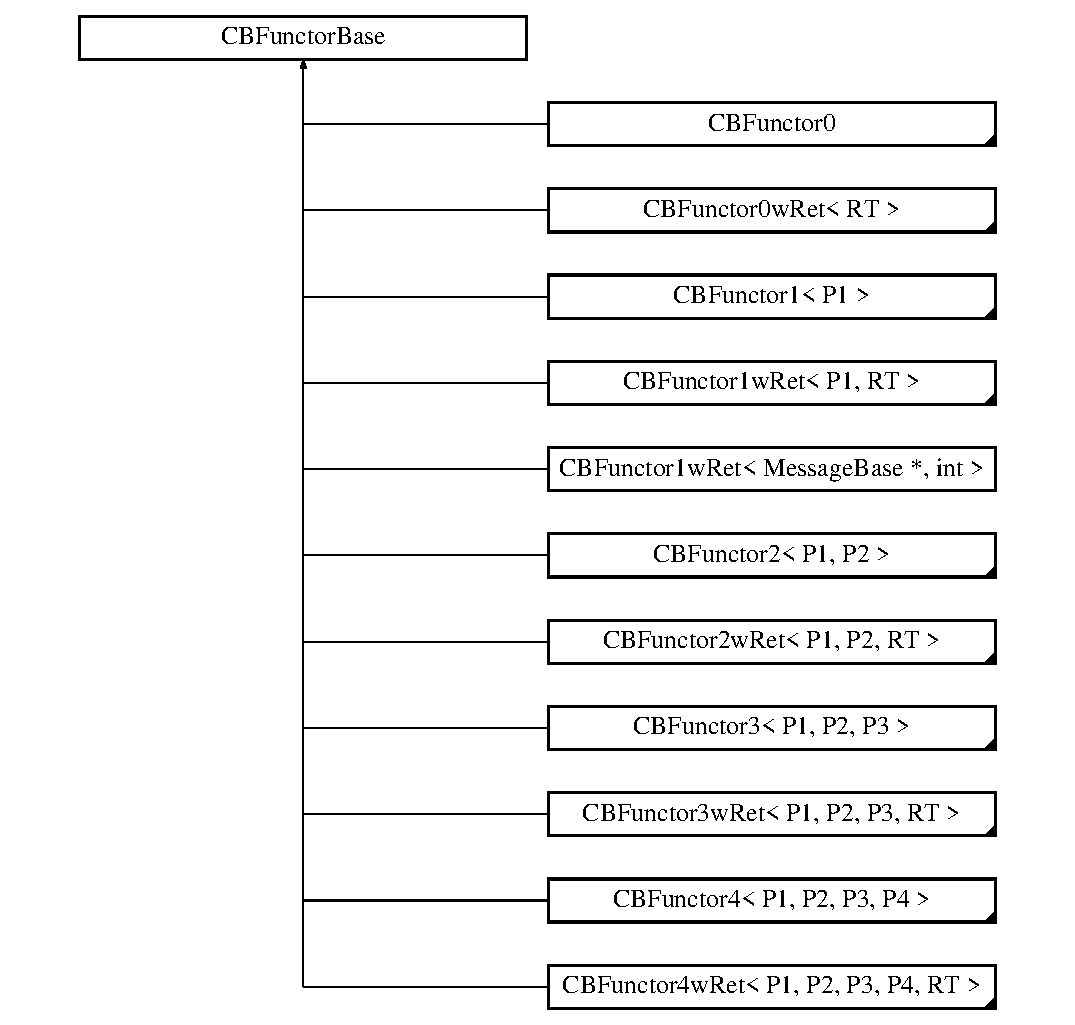
\includegraphics[height=12.000000cm]{classCBFunctorBase}
\end{center}
\end{figure}
\subsection*{Classes}
\begin{DoxyCompactItemize}
\item 
class {\bf Dummy\+Init}
\end{DoxyCompactItemize}
\subsection*{Public Types}
\begin{DoxyCompactItemize}
\item 
enum \{ {\bfseries M\+E\+M\+\_\+\+F\+U\+N\+C\+\_\+\+S\+I\+ZE} = sizeof(P\+Mem\+Func)
 \}\label{classCBFunctorBase_abd5a4f1e7a01526a7531a0a10baea05a}

\item 
typedef void(C\+B\+Functor\+Base\+::$\ast$ {\bfseries P\+Mem\+Func}) ()\label{classCBFunctorBase_a0b6994a0ae24a0179f34884c3b3b1f81}

\item 
typedef void($\ast$ {\bfseries P\+Func}) ()\label{classCBFunctorBase_a4f0b9826c15d940e073292ce7bfae312}

\end{DoxyCompactItemize}
\subsection*{Public Member Functions}
\begin{DoxyCompactItemize}
\item 
{\bfseries operator R\+H\+C\+B\+\_\+\+B\+O\+OL} () const \label{classCBFunctorBase_af34a298bd07b00a2c7a89c98e7b96f79}

\item 
P\+Func {\bfseries get\+Func} () const \label{classCBFunctorBase_a6429f4fb4cedd4d37f9dac39e93e4e21}

\item 
void $\ast$ {\bfseries get\+Callee} () const \label{classCBFunctorBase_a914255b831c1278ba0587b7496a08313}

\item 
const char $\ast$ {\bfseries get\+Mem\+Func} () const \label{classCBFunctorBase_a360081a2dde017999e385eff7448be64}

\end{DoxyCompactItemize}
\subsection*{Protected Member Functions}
\begin{DoxyCompactItemize}
\item 
{\bfseries C\+B\+Functor\+Base} (const void $\ast$c, P\+Func f, const void $\ast$mf, size\+\_\+t sz)\label{classCBFunctorBase_ad26c29cddb39d6b9767c2d04f9490e65}

\end{DoxyCompactItemize}
\subsection*{Protected Attributes}
\begin{DoxyCompactItemize}
\item 
void $\ast$ {\bfseries callee}\label{classCBFunctorBase_a4350b45a3bc31a07ef188c61ee7af584}

\item 
\begin{tabbing}
xx\=xx\=xx\=xx\=xx\=xx\=xx\=xx\=xx\=\kill
union \{\\
\>PFunc {\bfseries func}\\
\>char {\bfseries memFunc} [MEM\_FUNC\_SIZE]\\
\}; \label{classCBFunctorBase_af130b02d1cd0d194b552c70725830164}
\\

\end{tabbing}\end{DoxyCompactItemize}
\subsection*{Friends}
\begin{DoxyCompactItemize}
\item 
R\+H\+C\+B\+\_\+\+B\+O\+OL {\bfseries operator==} (const {\bf C\+B\+Functor\+Base} \&lhs, const {\bf C\+B\+Functor\+Base} \&rhs)\label{classCBFunctorBase_a227c0f351c0050b1d8c8fb5eb21fda4a}

\item 
R\+H\+C\+B\+\_\+\+B\+O\+OL {\bfseries operator!=} (const {\bf C\+B\+Functor\+Base} \&lhs, const {\bf C\+B\+Functor\+Base} \&rhs)\label{classCBFunctorBase_a71e018e8e95ad4ac2722f07bcf006fbc}

\item 
R\+H\+C\+B\+\_\+\+B\+O\+OL {\bfseries operator$<$} (const {\bf C\+B\+Functor\+Base} \&lhs, const {\bf C\+B\+Functor\+Base} \&rhs)\label{classCBFunctorBase_a34ea68bc41f2e609f96a31cc6c224c70}

\end{DoxyCompactItemize}


The documentation for this class was generated from the following file\+:\begin{DoxyCompactItemize}
\item 
Callback.\+h\end{DoxyCompactItemize}

\section{C\+B\+Member\+Of1st\+Arg\+Translator1$<$ P1, Mem\+Func $>$ Class Template Reference}
\label{classCBMemberOf1stArgTranslator1}\index{C\+B\+Member\+Of1st\+Arg\+Translator1$<$ P1, Mem\+Func $>$@{C\+B\+Member\+Of1st\+Arg\+Translator1$<$ P1, Mem\+Func $>$}}
Inheritance diagram for C\+B\+Member\+Of1st\+Arg\+Translator1$<$ P1, Mem\+Func $>$\+:\begin{figure}[H]
\begin{center}
\leavevmode
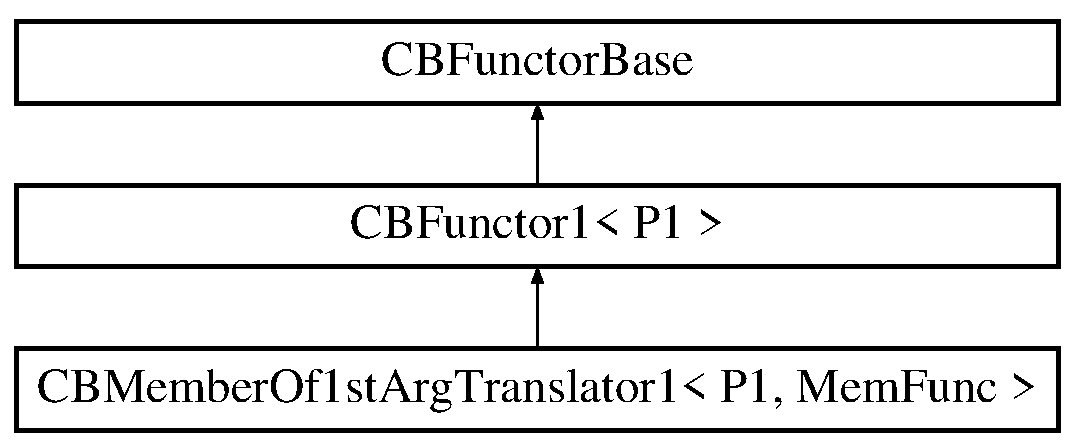
\includegraphics[height=3.000000cm]{classCBMemberOf1stArgTranslator1}
\end{center}
\end{figure}
\subsection*{Public Member Functions}
\begin{DoxyCompactItemize}
\item 
{\bfseries C\+B\+Member\+Of1st\+Arg\+Translator1} (const Mem\+Func \&m)\label{classCBMemberOf1stArgTranslator1_ab49120b3b5bff2dd8e6d4ffedf37d9be}

\end{DoxyCompactItemize}
\subsection*{Static Public Member Functions}
\begin{DoxyCompactItemize}
\item 
static void {\bfseries thunk} (const {\bf C\+B\+Functor\+Base} \&ftor, P1 p1)\label{classCBMemberOf1stArgTranslator1_a8d0d7551febbaad74a7b5871e13ec5aa}

\end{DoxyCompactItemize}
\subsection*{Additional Inherited Members}


The documentation for this class was generated from the following file\+:\begin{DoxyCompactItemize}
\item 
Callback.\+h\end{DoxyCompactItemize}

\section{C\+B\+Member\+Of1st\+Arg\+Translator1w\+Ret$<$ P1, RT, Mem\+Func $>$ Class Template Reference}
\label{classCBMemberOf1stArgTranslator1wRet}\index{C\+B\+Member\+Of1st\+Arg\+Translator1w\+Ret$<$ P1, R\+T, Mem\+Func $>$@{C\+B\+Member\+Of1st\+Arg\+Translator1w\+Ret$<$ P1, R\+T, Mem\+Func $>$}}
Inheritance diagram for C\+B\+Member\+Of1st\+Arg\+Translator1w\+Ret$<$ P1, RT, Mem\+Func $>$\+:\begin{figure}[H]
\begin{center}
\leavevmode
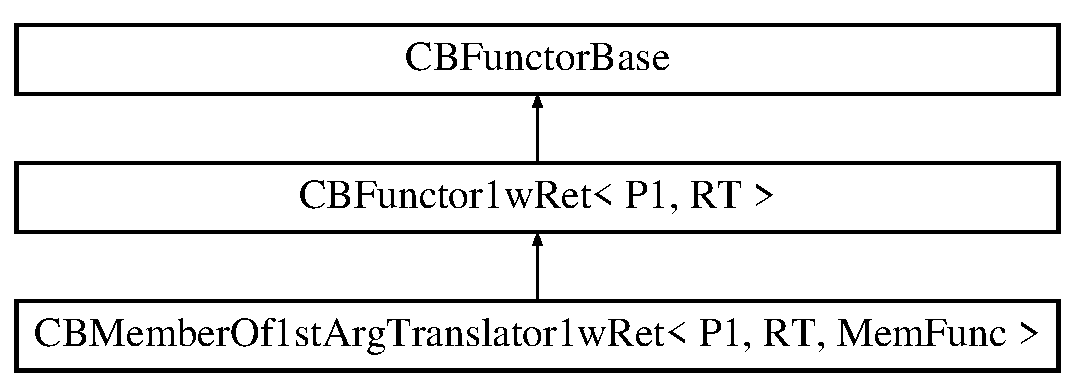
\includegraphics[height=3.000000cm]{classCBMemberOf1stArgTranslator1wRet}
\end{center}
\end{figure}
\subsection*{Public Member Functions}
\begin{DoxyCompactItemize}
\item 
{\bfseries C\+B\+Member\+Of1st\+Arg\+Translator1w\+Ret} (const Mem\+Func \&m)\label{classCBMemberOf1stArgTranslator1wRet_a6caa8b74e38357ffe68b38662fc97731}

\end{DoxyCompactItemize}
\subsection*{Static Public Member Functions}
\begin{DoxyCompactItemize}
\item 
static RT {\bfseries thunk} (const {\bf C\+B\+Functor\+Base} \&ftor, P1 p1)\label{classCBMemberOf1stArgTranslator1wRet_ab4fcb6d97e3ff9f87f0348822b3926d5}

\end{DoxyCompactItemize}
\subsection*{Additional Inherited Members}


The documentation for this class was generated from the following file\+:\begin{DoxyCompactItemize}
\item 
Callback.\+h\end{DoxyCompactItemize}

\section{C\+B\+Member\+Of1st\+Arg\+Translator2$<$ P1, P2, Mem\+Func $>$ Class Template Reference}
\label{classCBMemberOf1stArgTranslator2}\index{C\+B\+Member\+Of1st\+Arg\+Translator2$<$ P1, P2, Mem\+Func $>$@{C\+B\+Member\+Of1st\+Arg\+Translator2$<$ P1, P2, Mem\+Func $>$}}
Inheritance diagram for C\+B\+Member\+Of1st\+Arg\+Translator2$<$ P1, P2, Mem\+Func $>$\+:\begin{figure}[H]
\begin{center}
\leavevmode
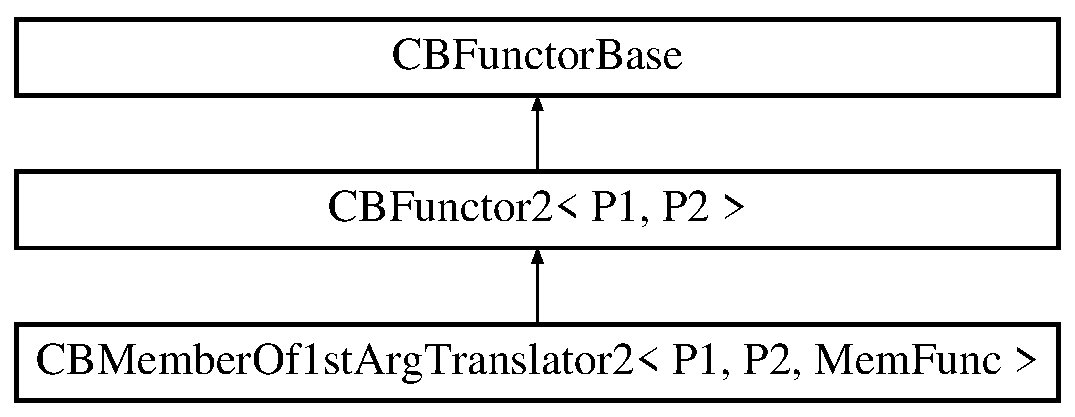
\includegraphics[height=3.000000cm]{classCBMemberOf1stArgTranslator2}
\end{center}
\end{figure}
\subsection*{Public Member Functions}
\begin{DoxyCompactItemize}
\item 
{\bfseries C\+B\+Member\+Of1st\+Arg\+Translator2} (const Mem\+Func \&m)\label{classCBMemberOf1stArgTranslator2_a023911cf50561084aba2161ee7c62833}

\end{DoxyCompactItemize}
\subsection*{Static Public Member Functions}
\begin{DoxyCompactItemize}
\item 
static void {\bfseries thunk} (const {\bf C\+B\+Functor\+Base} \&ftor, P1 p1, P2 p2)\label{classCBMemberOf1stArgTranslator2_a19f52a3dbdd607f7ecd1a9096579a22e}

\end{DoxyCompactItemize}
\subsection*{Additional Inherited Members}


The documentation for this class was generated from the following file\+:\begin{DoxyCompactItemize}
\item 
Callback.\+h\end{DoxyCompactItemize}

\section{C\+B\+Member\+Of1st\+Arg\+Translator2w\+Ret$<$ P1, P2, RT, Mem\+Func $>$ Class Template Reference}
\label{classCBMemberOf1stArgTranslator2wRet}\index{C\+B\+Member\+Of1st\+Arg\+Translator2w\+Ret$<$ P1, P2, R\+T, Mem\+Func $>$@{C\+B\+Member\+Of1st\+Arg\+Translator2w\+Ret$<$ P1, P2, R\+T, Mem\+Func $>$}}
Inheritance diagram for C\+B\+Member\+Of1st\+Arg\+Translator2w\+Ret$<$ P1, P2, RT, Mem\+Func $>$\+:\begin{figure}[H]
\begin{center}
\leavevmode
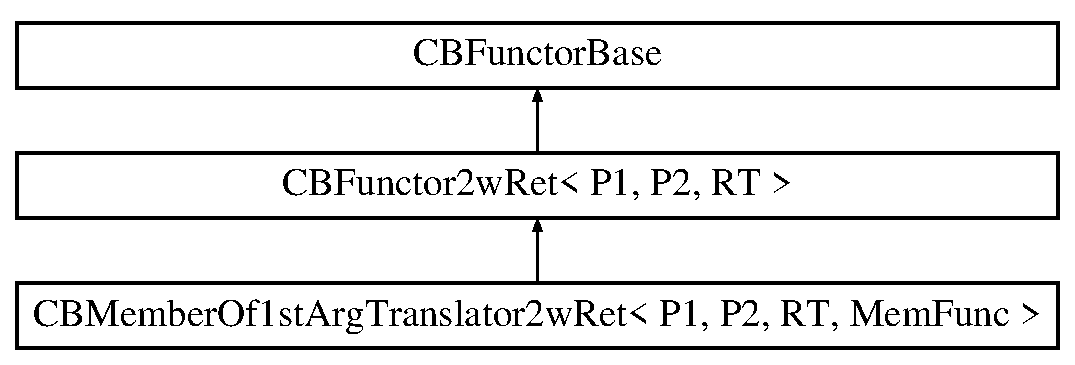
\includegraphics[height=3.000000cm]{classCBMemberOf1stArgTranslator2wRet}
\end{center}
\end{figure}
\subsection*{Public Member Functions}
\begin{DoxyCompactItemize}
\item 
{\bfseries C\+B\+Member\+Of1st\+Arg\+Translator2w\+Ret} (const Mem\+Func \&m)\label{classCBMemberOf1stArgTranslator2wRet_a044a1350fb9f59ba8ec38ea59305ed8f}

\end{DoxyCompactItemize}
\subsection*{Static Public Member Functions}
\begin{DoxyCompactItemize}
\item 
static RT {\bfseries thunk} (const {\bf C\+B\+Functor\+Base} \&ftor, P1 p1, P2 p2)\label{classCBMemberOf1stArgTranslator2wRet_a441af3982061f212f00b6f2d91cb10d4}

\end{DoxyCompactItemize}
\subsection*{Additional Inherited Members}


The documentation for this class was generated from the following file\+:\begin{DoxyCompactItemize}
\item 
Callback.\+h\end{DoxyCompactItemize}

\section{C\+B\+Member\+Of1st\+Arg\+Translator3$<$ P1, P2, P3, Mem\+Func $>$ Class Template Reference}
\label{classCBMemberOf1stArgTranslator3}\index{C\+B\+Member\+Of1st\+Arg\+Translator3$<$ P1, P2, P3, Mem\+Func $>$@{C\+B\+Member\+Of1st\+Arg\+Translator3$<$ P1, P2, P3, Mem\+Func $>$}}
Inheritance diagram for C\+B\+Member\+Of1st\+Arg\+Translator3$<$ P1, P2, P3, Mem\+Func $>$\+:\begin{figure}[H]
\begin{center}
\leavevmode
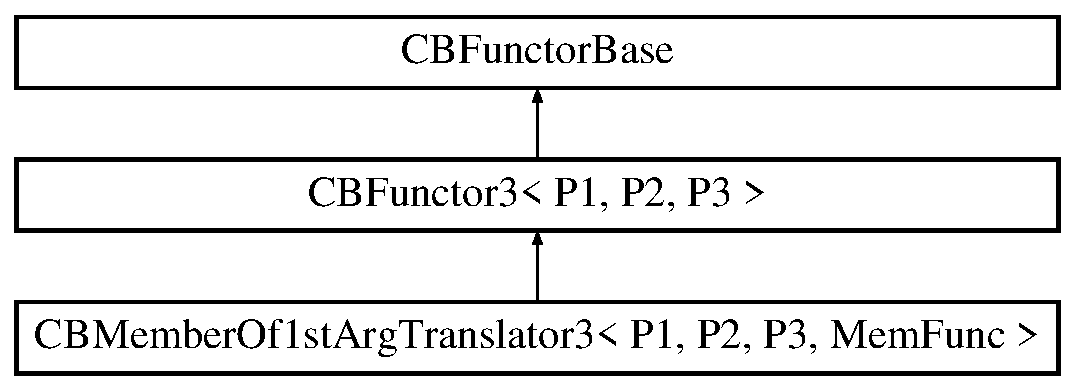
\includegraphics[height=3.000000cm]{classCBMemberOf1stArgTranslator3}
\end{center}
\end{figure}
\subsection*{Public Member Functions}
\begin{DoxyCompactItemize}
\item 
{\bfseries C\+B\+Member\+Of1st\+Arg\+Translator3} (const Mem\+Func \&m)\label{classCBMemberOf1stArgTranslator3_a0d0af6a625075314d7639aa6ed40c574}

\end{DoxyCompactItemize}
\subsection*{Static Public Member Functions}
\begin{DoxyCompactItemize}
\item 
static void {\bfseries thunk} (const {\bf C\+B\+Functor\+Base} \&ftor, P1 p1, P2 p2, P3 p3)\label{classCBMemberOf1stArgTranslator3_adb8aa106ab7d055c2088cb12b01669b5}

\end{DoxyCompactItemize}
\subsection*{Additional Inherited Members}


The documentation for this class was generated from the following file\+:\begin{DoxyCompactItemize}
\item 
Callback.\+h\end{DoxyCompactItemize}

\section{C\+B\+Member\+Of1st\+Arg\+Translator3w\+Ret$<$ P1, P2, P3, RT, Mem\+Func $>$ Class Template Reference}
\label{classCBMemberOf1stArgTranslator3wRet}\index{C\+B\+Member\+Of1st\+Arg\+Translator3w\+Ret$<$ P1, P2, P3, R\+T, Mem\+Func $>$@{C\+B\+Member\+Of1st\+Arg\+Translator3w\+Ret$<$ P1, P2, P3, R\+T, Mem\+Func $>$}}
Inheritance diagram for C\+B\+Member\+Of1st\+Arg\+Translator3w\+Ret$<$ P1, P2, P3, RT, Mem\+Func $>$\+:\begin{figure}[H]
\begin{center}
\leavevmode
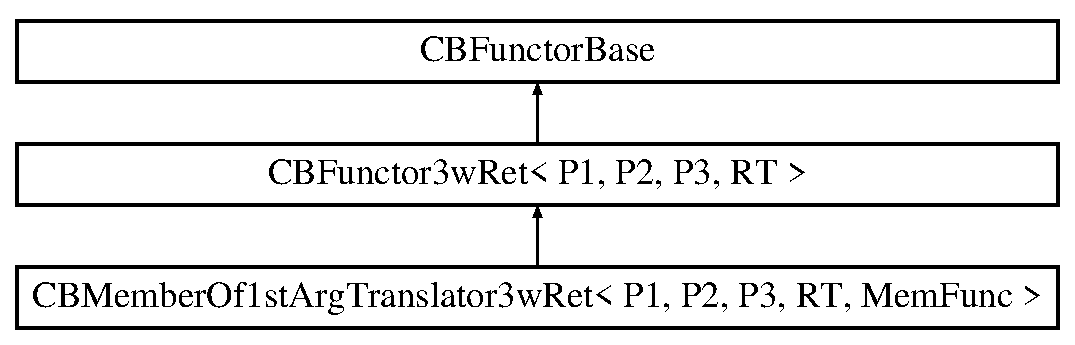
\includegraphics[height=3.000000cm]{classCBMemberOf1stArgTranslator3wRet}
\end{center}
\end{figure}
\subsection*{Public Member Functions}
\begin{DoxyCompactItemize}
\item 
{\bfseries C\+B\+Member\+Of1st\+Arg\+Translator3w\+Ret} (const Mem\+Func \&m)\label{classCBMemberOf1stArgTranslator3wRet_a1cc9c0e22254d70012d775811e803851}

\end{DoxyCompactItemize}
\subsection*{Static Public Member Functions}
\begin{DoxyCompactItemize}
\item 
static RT {\bfseries thunk} (const {\bf C\+B\+Functor\+Base} \&ftor, P1 p1, P2 p2, P3 p3)\label{classCBMemberOf1stArgTranslator3wRet_a76d2c43bcccf4bba447159433ad02a40}

\end{DoxyCompactItemize}
\subsection*{Additional Inherited Members}


The documentation for this class was generated from the following file\+:\begin{DoxyCompactItemize}
\item 
Callback.\+h\end{DoxyCompactItemize}

\section{C\+B\+Member\+Of1st\+Arg\+Translator4$<$ P1, P2, P3, P4, Mem\+Func $>$ Class Template Reference}
\label{classCBMemberOf1stArgTranslator4}\index{C\+B\+Member\+Of1st\+Arg\+Translator4$<$ P1, P2, P3, P4, Mem\+Func $>$@{C\+B\+Member\+Of1st\+Arg\+Translator4$<$ P1, P2, P3, P4, Mem\+Func $>$}}
Inheritance diagram for C\+B\+Member\+Of1st\+Arg\+Translator4$<$ P1, P2, P3, P4, Mem\+Func $>$\+:\begin{figure}[H]
\begin{center}
\leavevmode
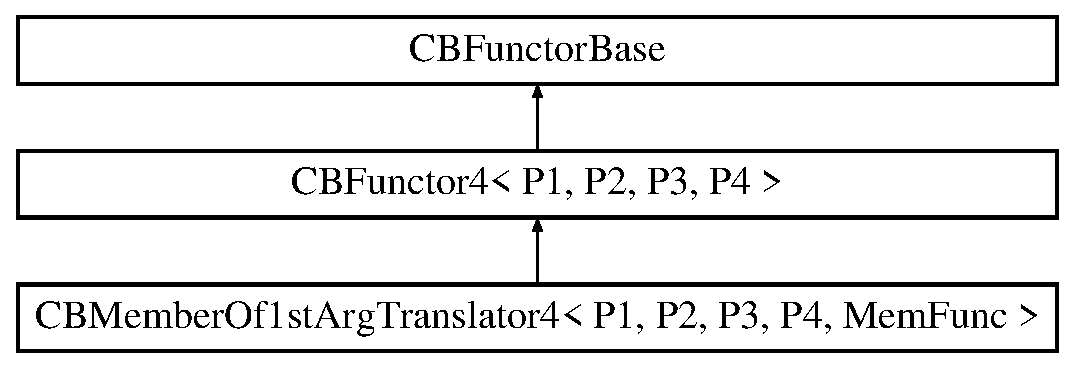
\includegraphics[height=3.000000cm]{classCBMemberOf1stArgTranslator4}
\end{center}
\end{figure}
\subsection*{Public Member Functions}
\begin{DoxyCompactItemize}
\item 
{\bfseries C\+B\+Member\+Of1st\+Arg\+Translator4} (const Mem\+Func \&m)\label{classCBMemberOf1stArgTranslator4_aaa496d239ea6144915739368a8007e3b}

\end{DoxyCompactItemize}
\subsection*{Static Public Member Functions}
\begin{DoxyCompactItemize}
\item 
static void {\bfseries thunk} (const {\bf C\+B\+Functor\+Base} \&ftor, P1 p1, P2 p2, P3 p3, P4 p4)\label{classCBMemberOf1stArgTranslator4_a6403ce84fe0adc0ffbd602c8d697a8b1}

\end{DoxyCompactItemize}
\subsection*{Additional Inherited Members}


The documentation for this class was generated from the following file\+:\begin{DoxyCompactItemize}
\item 
Callback.\+h\end{DoxyCompactItemize}

\section{C\+B\+Member\+Of1st\+Arg\+Translator4w\+Ret$<$ P1, P2, P3, P4, RT, Mem\+Func $>$ Class Template Reference}
\label{classCBMemberOf1stArgTranslator4wRet}\index{C\+B\+Member\+Of1st\+Arg\+Translator4w\+Ret$<$ P1, P2, P3, P4, R\+T, Mem\+Func $>$@{C\+B\+Member\+Of1st\+Arg\+Translator4w\+Ret$<$ P1, P2, P3, P4, R\+T, Mem\+Func $>$}}
Inheritance diagram for C\+B\+Member\+Of1st\+Arg\+Translator4w\+Ret$<$ P1, P2, P3, P4, RT, Mem\+Func $>$\+:\begin{figure}[H]
\begin{center}
\leavevmode
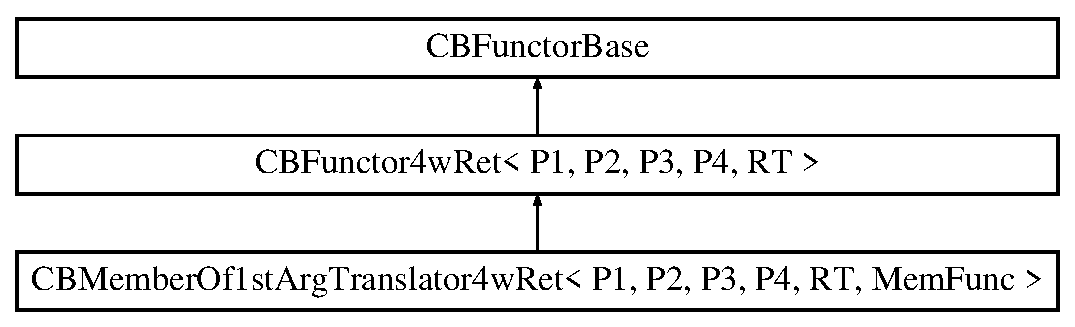
\includegraphics[height=3.000000cm]{classCBMemberOf1stArgTranslator4wRet}
\end{center}
\end{figure}
\subsection*{Public Member Functions}
\begin{DoxyCompactItemize}
\item 
{\bfseries C\+B\+Member\+Of1st\+Arg\+Translator4w\+Ret} (const Mem\+Func \&m)\label{classCBMemberOf1stArgTranslator4wRet_a26df225ad41821d1b66bbe2d52a1af49}

\end{DoxyCompactItemize}
\subsection*{Static Public Member Functions}
\begin{DoxyCompactItemize}
\item 
static RT {\bfseries thunk} (const {\bf C\+B\+Functor\+Base} \&ftor, P1 p1, P2 p2, P3 p3, P4 p4)\label{classCBMemberOf1stArgTranslator4wRet_a941353b6cd743478e22eb62bba0e4ca4}

\end{DoxyCompactItemize}
\subsection*{Additional Inherited Members}


The documentation for this class was generated from the following file\+:\begin{DoxyCompactItemize}
\item 
Callback.\+h\end{DoxyCompactItemize}

\section{C\+B\+Member\+Translator0$<$ Callee, Mem\+Func $>$ Class Template Reference}
\label{classCBMemberTranslator0}\index{C\+B\+Member\+Translator0$<$ Callee, Mem\+Func $>$@{C\+B\+Member\+Translator0$<$ Callee, Mem\+Func $>$}}
Inheritance diagram for C\+B\+Member\+Translator0$<$ Callee, Mem\+Func $>$\+:\begin{figure}[H]
\begin{center}
\leavevmode
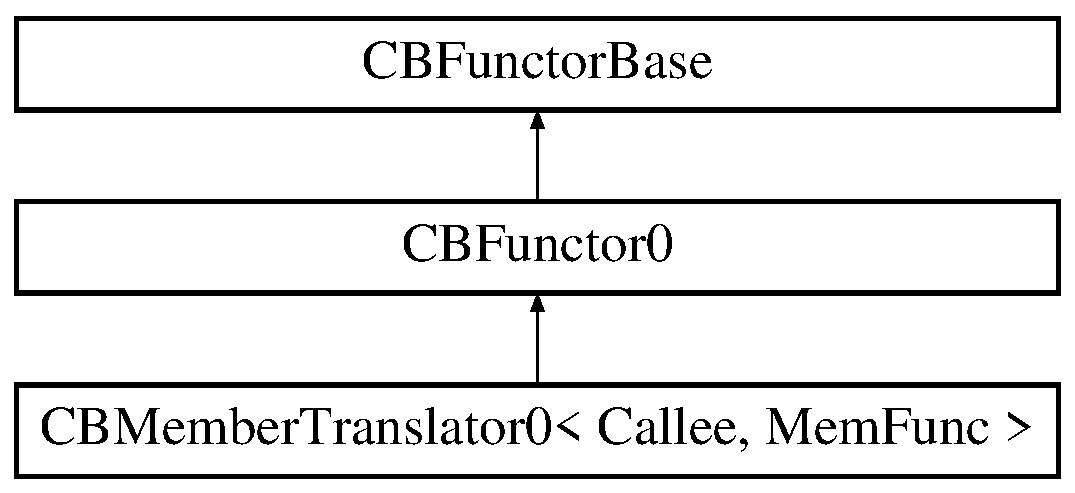
\includegraphics[height=3.000000cm]{classCBMemberTranslator0}
\end{center}
\end{figure}
\subsection*{Public Member Functions}
\begin{DoxyCompactItemize}
\item 
{\bfseries C\+B\+Member\+Translator0} (Callee \&c, const Mem\+Func \&m)\label{classCBMemberTranslator0_af242b8ca6be0ecabc13c0c9b8ae4a855}

\end{DoxyCompactItemize}
\subsection*{Static Public Member Functions}
\begin{DoxyCompactItemize}
\item 
static void {\bfseries thunk} (const {\bf C\+B\+Functor\+Base} \&ftor)\label{classCBMemberTranslator0_a0c48ec67cc966a40be1b0c47979f5cb5}

\end{DoxyCompactItemize}
\subsection*{Additional Inherited Members}


The documentation for this class was generated from the following file\+:\begin{DoxyCompactItemize}
\item 
Callback.\+h\end{DoxyCompactItemize}

\section{C\+B\+Member\+Translator0w\+Ret$<$ RT, Callee, Mem\+Func $>$ Class Template Reference}
\label{classCBMemberTranslator0wRet}\index{C\+B\+Member\+Translator0w\+Ret$<$ R\+T, Callee, Mem\+Func $>$@{C\+B\+Member\+Translator0w\+Ret$<$ R\+T, Callee, Mem\+Func $>$}}
Inheritance diagram for C\+B\+Member\+Translator0w\+Ret$<$ RT, Callee, Mem\+Func $>$\+:\begin{figure}[H]
\begin{center}
\leavevmode
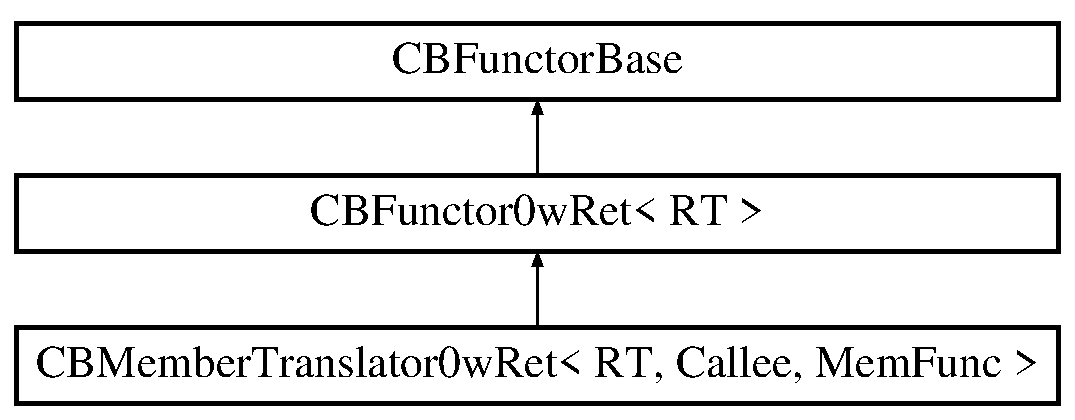
\includegraphics[height=3.000000cm]{classCBMemberTranslator0wRet}
\end{center}
\end{figure}
\subsection*{Public Member Functions}
\begin{DoxyCompactItemize}
\item 
{\bfseries C\+B\+Member\+Translator0w\+Ret} (Callee \&c, const Mem\+Func \&m)\label{classCBMemberTranslator0wRet_a009f4acc5619fd7cc15e9090eac4a170}

\end{DoxyCompactItemize}
\subsection*{Static Public Member Functions}
\begin{DoxyCompactItemize}
\item 
static RT {\bfseries thunk} (const {\bf C\+B\+Functor\+Base} \&ftor)\label{classCBMemberTranslator0wRet_a40506f0ca66be1d46686507963391617}

\end{DoxyCompactItemize}
\subsection*{Additional Inherited Members}


The documentation for this class was generated from the following file\+:\begin{DoxyCompactItemize}
\item 
Callback.\+h\end{DoxyCompactItemize}

\section{C\+B\+Member\+Translator1$<$ P1, Callee, Mem\+Func $>$ Class Template Reference}
\label{classCBMemberTranslator1}\index{C\+B\+Member\+Translator1$<$ P1, Callee, Mem\+Func $>$@{C\+B\+Member\+Translator1$<$ P1, Callee, Mem\+Func $>$}}
Inheritance diagram for C\+B\+Member\+Translator1$<$ P1, Callee, Mem\+Func $>$\+:\begin{figure}[H]
\begin{center}
\leavevmode
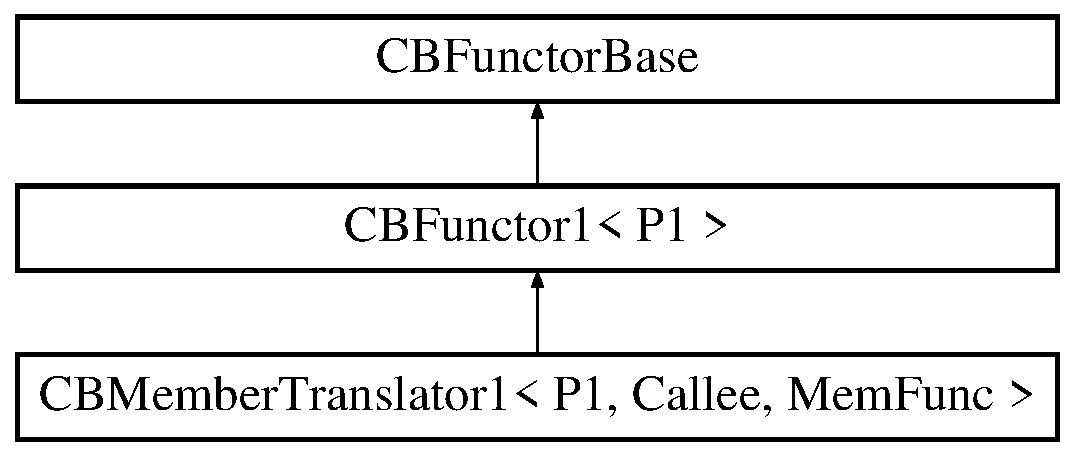
\includegraphics[height=3.000000cm]{classCBMemberTranslator1}
\end{center}
\end{figure}
\subsection*{Public Member Functions}
\begin{DoxyCompactItemize}
\item 
{\bfseries C\+B\+Member\+Translator1} (Callee \&c, const Mem\+Func \&m)\label{classCBMemberTranslator1_ab7349f1696db7d061f6a712a50c44f6b}

\end{DoxyCompactItemize}
\subsection*{Static Public Member Functions}
\begin{DoxyCompactItemize}
\item 
static void {\bfseries thunk} (const {\bf C\+B\+Functor\+Base} \&ftor, P1 p1)\label{classCBMemberTranslator1_a3946d0edab5f98a04d049f61b3b17b77}

\end{DoxyCompactItemize}
\subsection*{Additional Inherited Members}


The documentation for this class was generated from the following file\+:\begin{DoxyCompactItemize}
\item 
Callback.\+h\end{DoxyCompactItemize}

\section{C\+B\+Member\+Translator1w\+Ret$<$ P1, RT, Callee, Mem\+Func $>$ Class Template Reference}
\label{classCBMemberTranslator1wRet}\index{C\+B\+Member\+Translator1w\+Ret$<$ P1, R\+T, Callee, Mem\+Func $>$@{C\+B\+Member\+Translator1w\+Ret$<$ P1, R\+T, Callee, Mem\+Func $>$}}
Inheritance diagram for C\+B\+Member\+Translator1w\+Ret$<$ P1, RT, Callee, Mem\+Func $>$\+:\begin{figure}[H]
\begin{center}
\leavevmode
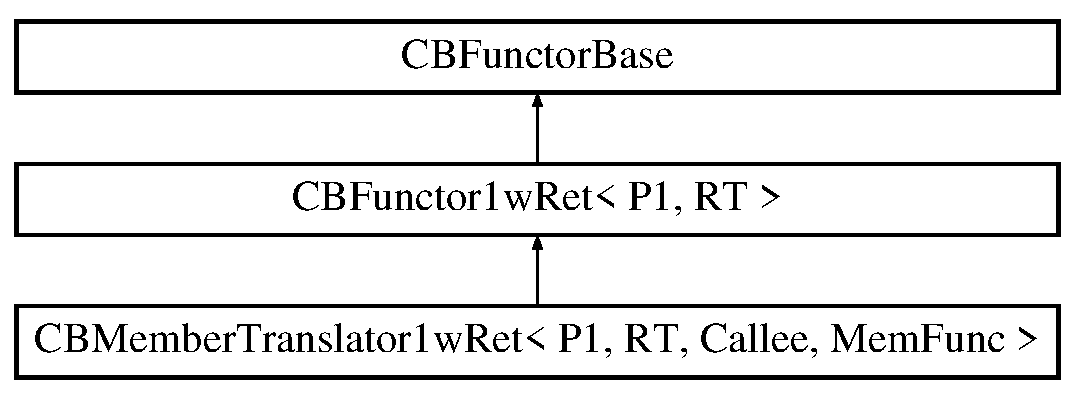
\includegraphics[height=3.000000cm]{classCBMemberTranslator1wRet}
\end{center}
\end{figure}
\subsection*{Public Member Functions}
\begin{DoxyCompactItemize}
\item 
{\bfseries C\+B\+Member\+Translator1w\+Ret} (Callee \&c, const Mem\+Func \&m)\label{classCBMemberTranslator1wRet_a38d17dfd10f274c581873edf4886c606}

\end{DoxyCompactItemize}
\subsection*{Static Public Member Functions}
\begin{DoxyCompactItemize}
\item 
static RT {\bfseries thunk} (const {\bf C\+B\+Functor\+Base} \&ftor, P1 p1)\label{classCBMemberTranslator1wRet_ae2177eab2be5fd4837cb63cc35252a00}

\end{DoxyCompactItemize}
\subsection*{Additional Inherited Members}


The documentation for this class was generated from the following file\+:\begin{DoxyCompactItemize}
\item 
Callback.\+h\end{DoxyCompactItemize}

\section{C\+B\+Member\+Translator2$<$ P1, P2, Callee, Mem\+Func $>$ Class Template Reference}
\label{classCBMemberTranslator2}\index{C\+B\+Member\+Translator2$<$ P1, P2, Callee, Mem\+Func $>$@{C\+B\+Member\+Translator2$<$ P1, P2, Callee, Mem\+Func $>$}}
Inheritance diagram for C\+B\+Member\+Translator2$<$ P1, P2, Callee, Mem\+Func $>$\+:\begin{figure}[H]
\begin{center}
\leavevmode
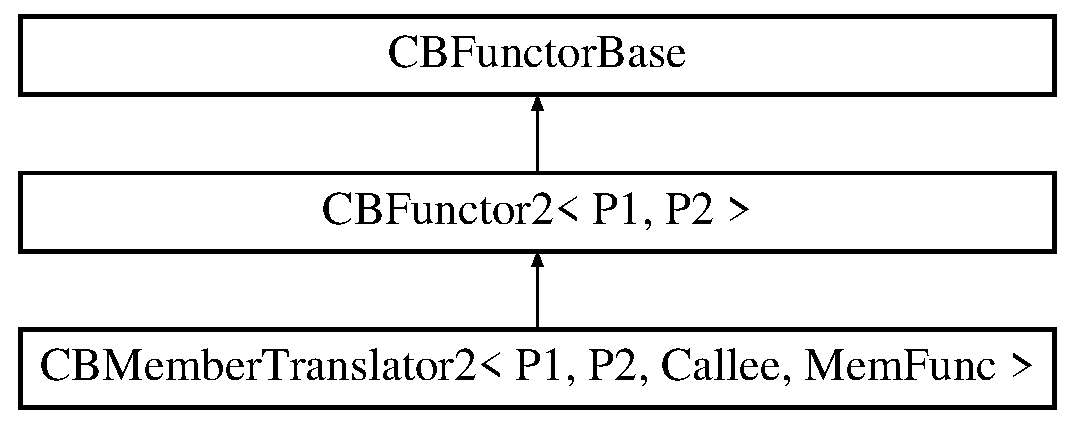
\includegraphics[height=3.000000cm]{classCBMemberTranslator2}
\end{center}
\end{figure}
\subsection*{Public Member Functions}
\begin{DoxyCompactItemize}
\item 
{\bfseries C\+B\+Member\+Translator2} (Callee \&c, const Mem\+Func \&m)\label{classCBMemberTranslator2_af8ffe32f73ed778d2f232a08127dc4cc}

\end{DoxyCompactItemize}
\subsection*{Static Public Member Functions}
\begin{DoxyCompactItemize}
\item 
static void {\bfseries thunk} (const {\bf C\+B\+Functor\+Base} \&ftor, P1 p1, P2 p2)\label{classCBMemberTranslator2_aaf39115b5d5157229b06a8be0e413b5d}

\end{DoxyCompactItemize}
\subsection*{Additional Inherited Members}


The documentation for this class was generated from the following file\+:\begin{DoxyCompactItemize}
\item 
Callback.\+h\end{DoxyCompactItemize}

\section{C\+B\+Member\+Translator2w\+Ret$<$ P1, P2, RT, Callee, Mem\+Func $>$ Class Template Reference}
\label{classCBMemberTranslator2wRet}\index{C\+B\+Member\+Translator2w\+Ret$<$ P1, P2, R\+T, Callee, Mem\+Func $>$@{C\+B\+Member\+Translator2w\+Ret$<$ P1, P2, R\+T, Callee, Mem\+Func $>$}}
Inheritance diagram for C\+B\+Member\+Translator2w\+Ret$<$ P1, P2, RT, Callee, Mem\+Func $>$\+:\begin{figure}[H]
\begin{center}
\leavevmode
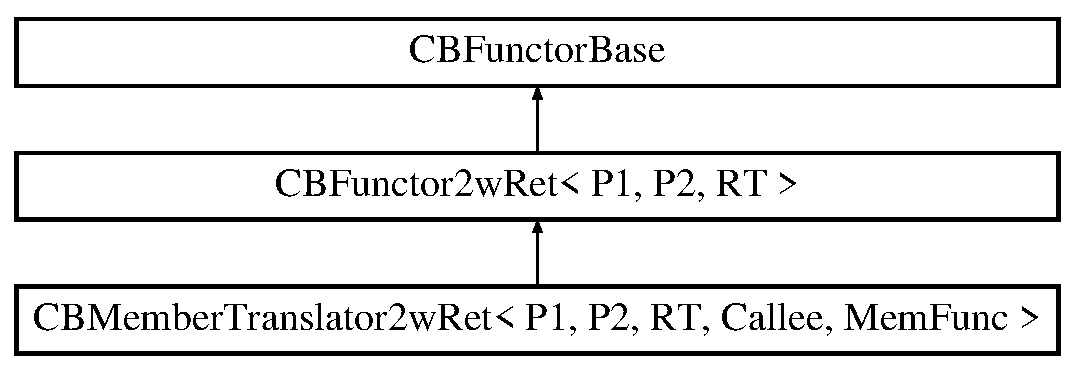
\includegraphics[height=3.000000cm]{classCBMemberTranslator2wRet}
\end{center}
\end{figure}
\subsection*{Public Member Functions}
\begin{DoxyCompactItemize}
\item 
{\bfseries C\+B\+Member\+Translator2w\+Ret} (Callee \&c, const Mem\+Func \&m)\label{classCBMemberTranslator2wRet_af4e5eb13ea4b7e03e101f26e5292ae6f}

\end{DoxyCompactItemize}
\subsection*{Static Public Member Functions}
\begin{DoxyCompactItemize}
\item 
static RT {\bfseries thunk} (const {\bf C\+B\+Functor\+Base} \&ftor, P1 p1, P2 p2)\label{classCBMemberTranslator2wRet_a0360f997fe211b042449357b0661aa2c}

\end{DoxyCompactItemize}
\subsection*{Additional Inherited Members}


The documentation for this class was generated from the following file\+:\begin{DoxyCompactItemize}
\item 
Callback.\+h\end{DoxyCompactItemize}

\section{C\+B\+Member\+Translator3$<$ P1, P2, P3, Callee, Mem\+Func $>$ Class Template Reference}
\label{classCBMemberTranslator3}\index{C\+B\+Member\+Translator3$<$ P1, P2, P3, Callee, Mem\+Func $>$@{C\+B\+Member\+Translator3$<$ P1, P2, P3, Callee, Mem\+Func $>$}}
Inheritance diagram for C\+B\+Member\+Translator3$<$ P1, P2, P3, Callee, Mem\+Func $>$\+:\begin{figure}[H]
\begin{center}
\leavevmode
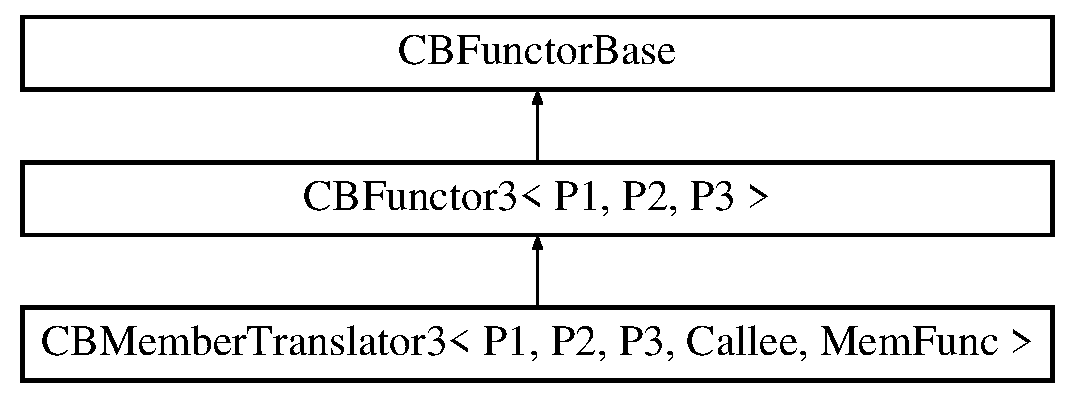
\includegraphics[height=3.000000cm]{classCBMemberTranslator3}
\end{center}
\end{figure}
\subsection*{Public Member Functions}
\begin{DoxyCompactItemize}
\item 
{\bfseries C\+B\+Member\+Translator3} (Callee \&c, const Mem\+Func \&m)\label{classCBMemberTranslator3_afbcd4fd12a4415a11738ff18aa4a1325}

\end{DoxyCompactItemize}
\subsection*{Static Public Member Functions}
\begin{DoxyCompactItemize}
\item 
static void {\bfseries thunk} (const {\bf C\+B\+Functor\+Base} \&ftor, P1 p1, P2 p2, P3 p3)\label{classCBMemberTranslator3_a05fe75348c3aaa930f6cc4f690c638f8}

\end{DoxyCompactItemize}
\subsection*{Additional Inherited Members}


The documentation for this class was generated from the following file\+:\begin{DoxyCompactItemize}
\item 
Callback.\+h\end{DoxyCompactItemize}

\section{C\+B\+Member\+Translator3w\+Ret$<$ P1, P2, P3, RT, Callee, Mem\+Func $>$ Class Template Reference}
\label{classCBMemberTranslator3wRet}\index{C\+B\+Member\+Translator3w\+Ret$<$ P1, P2, P3, R\+T, Callee, Mem\+Func $>$@{C\+B\+Member\+Translator3w\+Ret$<$ P1, P2, P3, R\+T, Callee, Mem\+Func $>$}}
Inheritance diagram for C\+B\+Member\+Translator3w\+Ret$<$ P1, P2, P3, RT, Callee, Mem\+Func $>$\+:\begin{figure}[H]
\begin{center}
\leavevmode
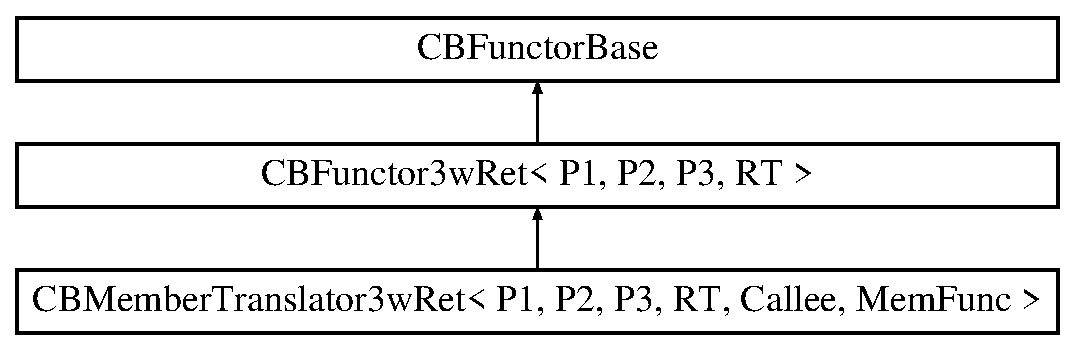
\includegraphics[height=3.000000cm]{classCBMemberTranslator3wRet}
\end{center}
\end{figure}
\subsection*{Public Member Functions}
\begin{DoxyCompactItemize}
\item 
{\bfseries C\+B\+Member\+Translator3w\+Ret} (Callee \&c, const Mem\+Func \&m)\label{classCBMemberTranslator3wRet_a71e2bbd6db9020a6b541a650ff7d81d5}

\end{DoxyCompactItemize}
\subsection*{Static Public Member Functions}
\begin{DoxyCompactItemize}
\item 
static RT {\bfseries thunk} (const {\bf C\+B\+Functor\+Base} \&ftor, P1 p1, P2 p2, P3 p3)\label{classCBMemberTranslator3wRet_a87eed002836701d52bf8f243c6fcc338}

\end{DoxyCompactItemize}
\subsection*{Additional Inherited Members}


The documentation for this class was generated from the following file\+:\begin{DoxyCompactItemize}
\item 
Callback.\+h\end{DoxyCompactItemize}

\section{C\+B\+Member\+Translator4$<$ P1, P2, P3, P4, Callee, Mem\+Func $>$ Class Template Reference}
\label{classCBMemberTranslator4}\index{C\+B\+Member\+Translator4$<$ P1, P2, P3, P4, Callee, Mem\+Func $>$@{C\+B\+Member\+Translator4$<$ P1, P2, P3, P4, Callee, Mem\+Func $>$}}
Inheritance diagram for C\+B\+Member\+Translator4$<$ P1, P2, P3, P4, Callee, Mem\+Func $>$\+:\begin{figure}[H]
\begin{center}
\leavevmode
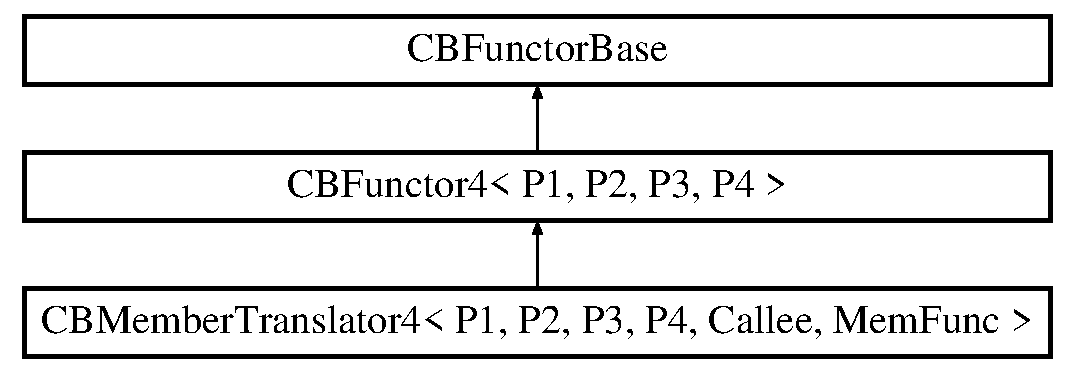
\includegraphics[height=3.000000cm]{classCBMemberTranslator4}
\end{center}
\end{figure}
\subsection*{Public Member Functions}
\begin{DoxyCompactItemize}
\item 
{\bfseries C\+B\+Member\+Translator4} (Callee \&c, const Mem\+Func \&m)\label{classCBMemberTranslator4_a5a36e912eb022c5d0b690c4b2b4d2437}

\end{DoxyCompactItemize}
\subsection*{Static Public Member Functions}
\begin{DoxyCompactItemize}
\item 
static void {\bfseries thunk} (const {\bf C\+B\+Functor\+Base} \&ftor, P1 p1, P2 p2, P3 p3, P4 p4)\label{classCBMemberTranslator4_a6921f84ba578024de5a49ab42d0529ff}

\end{DoxyCompactItemize}
\subsection*{Additional Inherited Members}


The documentation for this class was generated from the following file\+:\begin{DoxyCompactItemize}
\item 
Callback.\+h\end{DoxyCompactItemize}

\section{C\+B\+Member\+Translator4w\+Ret$<$ P1, P2, P3, P4, RT, Callee, Mem\+Func $>$ Class Template Reference}
\label{classCBMemberTranslator4wRet}\index{C\+B\+Member\+Translator4w\+Ret$<$ P1, P2, P3, P4, R\+T, Callee, Mem\+Func $>$@{C\+B\+Member\+Translator4w\+Ret$<$ P1, P2, P3, P4, R\+T, Callee, Mem\+Func $>$}}
Inheritance diagram for C\+B\+Member\+Translator4w\+Ret$<$ P1, P2, P3, P4, RT, Callee, Mem\+Func $>$\+:\begin{figure}[H]
\begin{center}
\leavevmode
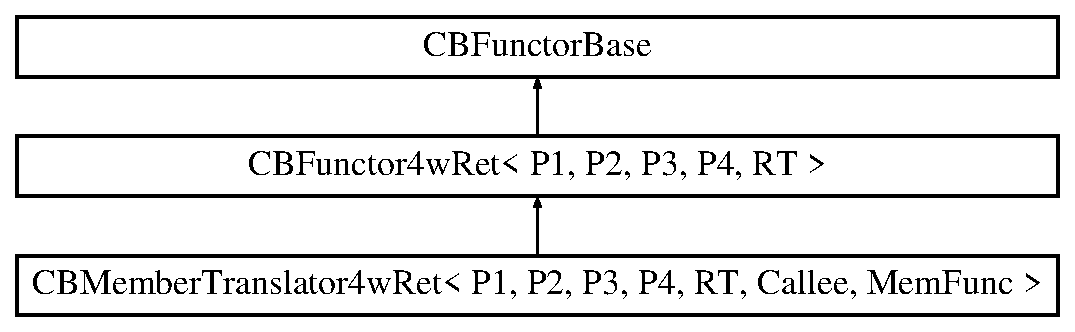
\includegraphics[height=3.000000cm]{classCBMemberTranslator4wRet}
\end{center}
\end{figure}
\subsection*{Public Member Functions}
\begin{DoxyCompactItemize}
\item 
{\bfseries C\+B\+Member\+Translator4w\+Ret} (Callee \&c, const Mem\+Func \&m)\label{classCBMemberTranslator4wRet_adccf77b2f6c7b9badb20795db06fcbb7}

\end{DoxyCompactItemize}
\subsection*{Static Public Member Functions}
\begin{DoxyCompactItemize}
\item 
static RT {\bfseries thunk} (const {\bf C\+B\+Functor\+Base} \&ftor, P1 p1, P2 p2, P3 p3, P4 p4)\label{classCBMemberTranslator4wRet_a5f094d9638e1327854be28cb2edcad68}

\end{DoxyCompactItemize}
\subsection*{Additional Inherited Members}


The documentation for this class was generated from the following file\+:\begin{DoxyCompactItemize}
\item 
Callback.\+h\end{DoxyCompactItemize}

\section{Connection\+Set Class Reference}
\label{classConnectionSet}\index{Connection\+Set@{Connection\+Set}}
\subsection*{Public Member Functions}
\begin{DoxyCompactItemize}
\item 
{\bf Connection\+Set} (string connection\+Set\+Name)
\item 
virtual {\bf $\sim$\+Connection\+Set} ()
\item 
void {\bf set\+Userid} (string userid)
\item 
void {\bf set\+Password} (string password)
\item 
void {\bf set\+Driver\+Name} (string driver\+Name)
\item 
void {\bf set\+Connection\+Type} (Connection\+Set\+Type connection\+Type)
\item 
void {\bf set\+Connection\+String} (string connection\+String)
\item 
void {\bf set\+Number\+Connections} (int number\+Connections)
\item 
void {\bf set\+D\+SN} (string dsn)
\item 
int {\bf perform\+Activation} ()
\item 
int {\bf perform\+Deactivation} ()
\item 
{\bf Db\+Connection\+Handle} $\ast$ {\bf reserve\+Connection} ()
\item 
{\bf Db\+Connection\+Handle} $\ast$ {\bf reserve\+Connection\+Non\+Blocking} ()
\item 
void {\bf release\+Connection} ({\bf Db\+Connection\+Handle} $\ast$connection\+Handle)
\item 
string {\bf to\+String} ()
\end{DoxyCompactItemize}


\subsection{Constructor \& Destructor Documentation}
\index{Connection\+Set@{Connection\+Set}!Connection\+Set@{Connection\+Set}}
\index{Connection\+Set@{Connection\+Set}!Connection\+Set@{Connection\+Set}}
\subsubsection[{Connection\+Set(string connection\+Set\+Name)}]{\setlength{\rightskip}{0pt plus 5cm}Connection\+Set\+::\+Connection\+Set (
\begin{DoxyParamCaption}
\item[{string}]{connection\+Set\+Name}
\end{DoxyParamCaption}
)}\label{classConnectionSet_ab0f18ac729ec5249880e72f56570f890}
Constructor \index{Connection\+Set@{Connection\+Set}!````~Connection\+Set@{$\sim$\+Connection\+Set}}
\index{````~Connection\+Set@{$\sim$\+Connection\+Set}!Connection\+Set@{Connection\+Set}}
\subsubsection[{$\sim$\+Connection\+Set()}]{\setlength{\rightskip}{0pt plus 5cm}Connection\+Set\+::$\sim$\+Connection\+Set (
\begin{DoxyParamCaption}
{}
\end{DoxyParamCaption}
)\hspace{0.3cm}{\ttfamily [virtual]}}\label{classConnectionSet_a13c8dfda9f89cb17389a82fb569a6f7d}
Virtual Destructor 

\subsection{Member Function Documentation}
\index{Connection\+Set@{Connection\+Set}!perform\+Activation@{perform\+Activation}}
\index{perform\+Activation@{perform\+Activation}!Connection\+Set@{Connection\+Set}}
\subsubsection[{perform\+Activation()}]{\setlength{\rightskip}{0pt plus 5cm}int Connection\+Set\+::perform\+Activation (
\begin{DoxyParamCaption}
{}
\end{DoxyParamCaption}
)}\label{classConnectionSet_a01ecb404e2cfd2a68284219c00cf419f}
Perform activation for the connection set. This includes connection establishment, error handling, and creation of the \doxyref{O\+PM}{p.}{classOPM} pool for storing the active connections. \begin{DoxyReturn}{Returns}
E\+R\+R\+OR upon failure; otherwise OK 
\end{DoxyReturn}


References O\+P\+M\+::create\+Pool(), Pg\+Connection\+::initialize(), and Db\+Connection\+Handle\+::initialize().

\index{Connection\+Set@{Connection\+Set}!perform\+Deactivation@{perform\+Deactivation}}
\index{perform\+Deactivation@{perform\+Deactivation}!Connection\+Set@{Connection\+Set}}
\subsubsection[{perform\+Deactivation()}]{\setlength{\rightskip}{0pt plus 5cm}int Connection\+Set\+::perform\+Deactivation (
\begin{DoxyParamCaption}
{}
\end{DoxyParamCaption}
)}\label{classConnectionSet_aecb7cde4d547c24dcc62c9303c1d718d}
Perform deactivation of the connection set. This should include connection tear down, error handling, and destruction of the \doxyref{O\+PM}{p.}{classOPM} pool for the connections, but currently there is no \doxyref{O\+PM}{p.}{classOPM} support for deallocating the pool of objects. We can loop through all of the \textquotesingle{}Available\textquotesingle{} connection objects and perform a disconnect/shutdown. H\+O\+W\+E\+V\+ER, this does assume that the application has released all of the connection objects back into the pool already (so that we can re-\/reserve them here). \begin{DoxyReturn}{Returns}
E\+R\+R\+OR upon failure; otherwise OK 
\end{DoxyReturn}


References reserve\+Connection\+Non\+Blocking(), and Db\+Connection\+Handle\+::shutdown().

\index{Connection\+Set@{Connection\+Set}!release\+Connection@{release\+Connection}}
\index{release\+Connection@{release\+Connection}!Connection\+Set@{Connection\+Set}}
\subsubsection[{release\+Connection(\+Db\+Connection\+Handle $\ast$connection\+Handle)}]{\setlength{\rightskip}{0pt plus 5cm}void Connection\+Set\+::release\+Connection (
\begin{DoxyParamCaption}
\item[{{\bf Db\+Connection\+Handle} $\ast$}]{connection\+Handle}
\end{DoxyParamCaption}
)}\label{classConnectionSet_aff9af59b568080969423771044ca7987}
Method to release the \doxyref{Db\+Connection}{p.}{classDbConnection} back into the Connection Set pool. This method is called from the similarly named static method in the \doxyref{Data\+Manager}{p.}{classDataManager}. \index{Connection\+Set@{Connection\+Set}!reserve\+Connection@{reserve\+Connection}}
\index{reserve\+Connection@{reserve\+Connection}!Connection\+Set@{Connection\+Set}}
\subsubsection[{reserve\+Connection()}]{\setlength{\rightskip}{0pt plus 5cm}{\bf Db\+Connection\+Handle} $\ast$ Connection\+Set\+::reserve\+Connection (
\begin{DoxyParamCaption}
{}
\end{DoxyParamCaption}
)}\label{classConnectionSet_a357ba80f870d459bfeb87a06e56ebd84}
Method to retrieve a pointer to a \doxyref{Db\+Connection}{p.}{classDbConnection} from the Connection Set pool. This method blocks until a \doxyref{Db\+Connection}{p.}{classDbConnection} becomes available if they are all currently in use. This method is called from the similarly named static method in the \doxyref{Data\+Manager}{p.}{classDataManager}. \index{Connection\+Set@{Connection\+Set}!reserve\+Connection\+Non\+Blocking@{reserve\+Connection\+Non\+Blocking}}
\index{reserve\+Connection\+Non\+Blocking@{reserve\+Connection\+Non\+Blocking}!Connection\+Set@{Connection\+Set}}
\subsubsection[{reserve\+Connection\+Non\+Blocking()}]{\setlength{\rightskip}{0pt plus 5cm}{\bf Db\+Connection\+Handle} $\ast$ Connection\+Set\+::reserve\+Connection\+Non\+Blocking (
\begin{DoxyParamCaption}
{}
\end{DoxyParamCaption}
)}\label{classConnectionSet_ae3b561a55e5ca7c3c42c2bbd7aee7526}
Method to retrieve a pointer to a \doxyref{Db\+Connection}{p.}{classDbConnection} from the Connection Set pool. This method does N\+OT block if there are no Db\+Connections available in the pool. N\+O\+TE that the pools are configured not to G\+R\+OW and/or S\+H\+R\+I\+NK. This method is called from the similarly named static method in the \doxyref{Data\+Manager}{p.}{classDataManager}. \begin{DoxyReturn}{Returns}
N\+U\+LL if no \doxyref{Db\+Connection}{p.}{classDbConnection} available 
\end{DoxyReturn}


Referenced by perform\+Deactivation().

\index{Connection\+Set@{Connection\+Set}!set\+Connection\+String@{set\+Connection\+String}}
\index{set\+Connection\+String@{set\+Connection\+String}!Connection\+Set@{Connection\+Set}}
\subsubsection[{set\+Connection\+String(string connection\+String)}]{\setlength{\rightskip}{0pt plus 5cm}void Connection\+Set\+::set\+Connection\+String (
\begin{DoxyParamCaption}
\item[{string}]{connection\+String}
\end{DoxyParamCaption}
)}\label{classConnectionSet_abc08544f0395b1a35367872ca276b1d8}
Set the Connection String associated with the connection 

Referenced by Data\+Manager\+::initialize().

\index{Connection\+Set@{Connection\+Set}!set\+Connection\+Type@{set\+Connection\+Type}}
\index{set\+Connection\+Type@{set\+Connection\+Type}!Connection\+Set@{Connection\+Set}}
\subsubsection[{set\+Connection\+Type(\+Connection\+Set\+Type connection\+Type)}]{\setlength{\rightskip}{0pt plus 5cm}void Connection\+Set\+::set\+Connection\+Type (
\begin{DoxyParamCaption}
\item[{Connection\+Set\+Type}]{connection\+Type}
\end{DoxyParamCaption}
)}\label{classConnectionSet_ad5533cf5215822c5d2d6bf5cc80f4f7a}
Set the Connection Type associated with the connection 

Referenced by Data\+Manager\+::initialize().

\index{Connection\+Set@{Connection\+Set}!set\+Driver\+Name@{set\+Driver\+Name}}
\index{set\+Driver\+Name@{set\+Driver\+Name}!Connection\+Set@{Connection\+Set}}
\subsubsection[{set\+Driver\+Name(string driver\+Name)}]{\setlength{\rightskip}{0pt plus 5cm}void Connection\+Set\+::set\+Driver\+Name (
\begin{DoxyParamCaption}
\item[{string}]{driver\+Name}
\end{DoxyParamCaption}
)}\label{classConnectionSet_ab07115ff4da734387c98974c0dc095e9}
Set the Driver Name associated with the connection 

Referenced by Data\+Manager\+::initialize().

\index{Connection\+Set@{Connection\+Set}!set\+D\+SN@{set\+D\+SN}}
\index{set\+D\+SN@{set\+D\+SN}!Connection\+Set@{Connection\+Set}}
\subsubsection[{set\+D\+S\+N(string dsn)}]{\setlength{\rightskip}{0pt plus 5cm}void Connection\+Set\+::set\+D\+SN (
\begin{DoxyParamCaption}
\item[{string}]{dsn}
\end{DoxyParamCaption}
)}\label{classConnectionSet_a53b247274eda7c0297976fa254c5c54b}
Set the D\+SN 

Referenced by Data\+Manager\+::initialize().

\index{Connection\+Set@{Connection\+Set}!set\+Number\+Connections@{set\+Number\+Connections}}
\index{set\+Number\+Connections@{set\+Number\+Connections}!Connection\+Set@{Connection\+Set}}
\subsubsection[{set\+Number\+Connections(int number\+Connections)}]{\setlength{\rightskip}{0pt plus 5cm}void Connection\+Set\+::set\+Number\+Connections (
\begin{DoxyParamCaption}
\item[{int}]{number\+Connections}
\end{DoxyParamCaption}
)}\label{classConnectionSet_a5350522197adf3e40b5f722d93099666}
Set the number of connections 

Referenced by Data\+Manager\+::initialize().

\index{Connection\+Set@{Connection\+Set}!set\+Password@{set\+Password}}
\index{set\+Password@{set\+Password}!Connection\+Set@{Connection\+Set}}
\subsubsection[{set\+Password(string password)}]{\setlength{\rightskip}{0pt plus 5cm}void Connection\+Set\+::set\+Password (
\begin{DoxyParamCaption}
\item[{string}]{password}
\end{DoxyParamCaption}
)}\label{classConnectionSet_a55fbfb95bcc0591ed161acf90d8d29ff}
Set the Password associated with the connection 

Referenced by Data\+Manager\+::initialize().

\index{Connection\+Set@{Connection\+Set}!set\+Userid@{set\+Userid}}
\index{set\+Userid@{set\+Userid}!Connection\+Set@{Connection\+Set}}
\subsubsection[{set\+Userid(string userid)}]{\setlength{\rightskip}{0pt plus 5cm}void Connection\+Set\+::set\+Userid (
\begin{DoxyParamCaption}
\item[{string}]{userid}
\end{DoxyParamCaption}
)}\label{classConnectionSet_a52f6fbfe4741d5bbcf8b9d6846a32d46}
Set the Userid associated with the connection 

Referenced by Data\+Manager\+::initialize().

\index{Connection\+Set@{Connection\+Set}!to\+String@{to\+String}}
\index{to\+String@{to\+String}!Connection\+Set@{Connection\+Set}}
\subsubsection[{to\+String()}]{\setlength{\rightskip}{0pt plus 5cm}string Connection\+Set\+::to\+String (
\begin{DoxyParamCaption}
{}
\end{DoxyParamCaption}
)}\label{classConnectionSet_a2a46cf342aca5df44950cfbbde9f76d2}
String\textquotesingle{}ized debugging method \begin{DoxyReturn}{Returns}
string representation of the contents of this object 
\end{DoxyReturn}


The documentation for this class was generated from the following files\+:\begin{DoxyCompactItemize}
\item 
Connection\+Set.\+h\item 
Connection\+Set.\+cpp\end{DoxyCompactItemize}

\section{Conversions Class Reference}
\label{classConversions}\index{Conversions@{Conversions}}


{\ttfamily \#include $<$Conversions.\+h$>$}

\subsection*{Public Member Functions}
\begin{DoxyCompactItemize}
\item 
virtual {\bf $\sim$\+Conversions} ()
\end{DoxyCompactItemize}
\subsection*{Static Public Member Functions}
\begin{DoxyCompactItemize}
\item 
static string {\bf integer2\+Base} (unsigned long value, const unsigned int base)
\item 
static int {\bf binary2\+Decimal} (char $\ast$binary\+String)
\end{DoxyCompactItemize}


\subsection{Detailed Description}
\doxyref{Conversions}{p.}{classConversions} contains static conversion utility methods. 

\begin{DoxyParagraph}{Author}
Stephen Horton
\end{DoxyParagraph}
\begin{DoxyParagraph}{Revision}
1
\end{DoxyParagraph}


\subsection{Constructor \& Destructor Documentation}
\index{Conversions@{Conversions}!````~Conversions@{$\sim$\+Conversions}}
\index{````~Conversions@{$\sim$\+Conversions}!Conversions@{Conversions}}
\subsubsection[{$\sim$\+Conversions()}]{\setlength{\rightskip}{0pt plus 5cm}Conversions\+::$\sim$\+Conversions (
\begin{DoxyParamCaption}
{}
\end{DoxyParamCaption}
)\hspace{0.3cm}{\ttfamily [virtual]}}\label{classConversions_a9654fc95f53360d9d295fe34ff8ed593}
Virtual Destructor 

\subsection{Member Function Documentation}
\index{Conversions@{Conversions}!binary2\+Decimal@{binary2\+Decimal}}
\index{binary2\+Decimal@{binary2\+Decimal}!Conversions@{Conversions}}
\subsubsection[{binary2\+Decimal(char $\ast$binary\+String)}]{\setlength{\rightskip}{0pt plus 5cm}int Conversions\+::binary2\+Decimal (
\begin{DoxyParamCaption}
\item[{char $\ast$}]{binary\+String}
\end{DoxyParamCaption}
)\hspace{0.3cm}{\ttfamily [static]}}\label{classConversions_a638d11591da5f0baaabde89e31764245}
Convert a binary string to a decimal number. \begin{DoxyReturn}{Returns}
decimal value 
\end{DoxyReturn}
\index{Conversions@{Conversions}!integer2\+Base@{integer2\+Base}}
\index{integer2\+Base@{integer2\+Base}!Conversions@{Conversions}}
\subsubsection[{integer2\+Base(unsigned long value, const unsigned int base)}]{\setlength{\rightskip}{0pt plus 5cm}string Conversions\+::integer2\+Base (
\begin{DoxyParamCaption}
\item[{unsigned long}]{value, }
\item[{const unsigned int}]{base}
\end{DoxyParamCaption}
)\hspace{0.3cm}{\ttfamily [static]}}\label{classConversions_a8f67e3cca24e2bb862b34fc136757567}
Convert an integer to the specified Base. \begin{DoxyReturn}{Returns}
a string representation of the new Base value 
\end{DoxyReturn}


The documentation for this class was generated from the following files\+:\begin{DoxyCompactItemize}
\item 
Conversions.\+h\item 
Conversions.\+cpp\end{DoxyCompactItemize}

\section{Data\+Manager Class Reference}
\label{classDataManager}\index{Data\+Manager@{Data\+Manager}}


{\ttfamily \#include $<$Data\+Manager.\+h$>$}

\subsection*{Public Member Functions}
\begin{DoxyCompactItemize}
\item 
virtual {\bf $\sim$\+Data\+Manager} ()
\end{DoxyCompactItemize}
\subsection*{Static Public Member Functions}
\begin{DoxyCompactItemize}
\item 
static int {\bf initialize} (string configuration\+File\+Location)
\item 
static int {\bf activate\+Connection\+Set} (string connection\+Set\+Name)
\item 
static int {\bf de\+Activate\+Connection\+Set} (string connection\+Set\+Name)
\item 
static int {\bf de\+Activate\+All\+Connection\+Sets} ()
\item 
static {\bf Db\+Connection\+Handle} $\ast$ {\bf reserve\+Connection} (string connection\+Set\+Name)
\item 
static {\bf Db\+Connection\+Handle} $\ast$ {\bf reserve\+Connection\+Non\+Blocking} (string connection\+Set\+Name)
\item 
static void {\bf release\+Connection} ({\bf Db\+Connection\+Handle} $\ast$connection\+Handle)
\end{DoxyCompactItemize}


\subsection{Detailed Description}
\doxyref{Data\+Manager}{p.}{classDataManager} provides an application interface for setting and retrieving data to and from the persistent store. 

\doxyref{Data\+Manager}{p.}{classDataManager} is provided to hide some of the complexity of working with the database. It is intended to allow the database to be transparently replaced by different products/mechanisms without requiring the applications to do major surgery. Additionally, the \doxyref{Data\+Manager}{p.}{classDataManager} defines the concurrency model for how the applications will interact with the database. For example, an application program will have multiple threads; each thread requires periodic access to the database. A connection set will be created for this application that contains F\+E\+W\+ER connections than the number of threads that need them. Each thread is required to reserve a database connection, use it, and then release it back into the \doxyref{Data\+Manager}{p.}{classDataManager} pool so that another thread can then reserve and access. Of course the number of pooled connections versus the number of application threads is a systems engineering exercise and is configurable. Note that each connection is itself N\+OT thread safe and multiple threads should not attempt to access the same connection object (\doxyref{Db\+Connection\+Handle}{p.}{classDbConnectionHandle}) after it has been reserved by a single thread (this is typically the concurrency architecture for most database drivers). (This is possible with additional mutex/concurrency mechanisms implemented by the application, but it is N\+OT A\+D\+V\+I\+S\+A\+B\+LE, and not necessary). 

The general error handling strategy for the application developer should be as follows. If any errors are encountered while issuing query/update/insert/delete commands or while analyzing results, the developer should release the connection back into the pool and attempt to reserve another connection for use. The release process includes a health check on the connection that will attempt to re-\/establish/ renew that connection in the event of a failure. 

\doxyref{Data\+Manager}{p.}{classDataManager} exists as a library for each of the application processes to use for managing its database connections. \doxyref{Data\+Manager}{p.}{classDataManager} supports pooling of connections, and connection re-\/establishment and retry. Because the \doxyref{Data\+Manager}{p.}{classDataManager} is a bootstrap requirement for the applications obtaining all of their other configuration information (from the database), the \doxyref{Data\+Manager}{p.}{classDataManager} reads I\+TS configuration from a file. Furthermore, because \doxyref{Data\+Manager}{p.}{classDataManager} is used by multiple processes, this file must contain process-\/specific configuration sections to meet each process\textquotesingle{}s unique database connection requirements (with regards to the number of connections, both local and remote, etc.) 

The format of the \doxyref{Data\+Manager}{p.}{classDataManager} configuration file is\+: 
\begin{DoxyPre}
  [Configuration]
  DEBUGLEVEL=5
  ~\newline
~\newline

  [\doxyref{ConnectionSet}{p.}{classConnectionSet} Name]
  \# Some comments
  \# Perhaps some more comments
  USERID=userid
  PASSWORD=password (NOTE: This will need to be encrypted later...suggest MD5)
  DRIVERNAME=libpq
  CONNECTIONTYPE=LOCAL (or REMOTE)
  CONNECTIONSTRING="hostaddr=127.0.0.1 port=3180"
  NUMBERCONNECTIONS=1
  DSN=someDSN
  ~\newline
~\newline

  [Next \doxyref{ConnectionSet}{p.}{classConnectionSet} Name]
  ...
\end{DoxyPre}
 

The above [Configuration] section exists in order to set Data\+Manager-\/wide configuration parameters. Each subsequent [\doxyref{Connection\+Set}{p.}{classConnectionSet} Name] section establishes the configuration for a pool of connections. Note that an \doxyref{O\+PM}{p.}{classOPM} object pool is created even if only 1 connection is indicated. An application process can have multiple [\doxyref{Connection\+Set}{p.}{classConnectionSet}] sections for its use in the configuration file. The application process would then call \doxyref{Data\+Manager\+::activate\+Connection\+Set(string connection\+Set\+Name)}{p.}{classDataManager_a6c829d2c98f72e26edeae47bc777b4ad} for each configured connection set that it needs to use. 

\begin{DoxyParagraph}{Author}
Stephen Horton
\end{DoxyParagraph}
\begin{DoxyParagraph}{Revision}
1
\end{DoxyParagraph}


\subsection{Constructor \& Destructor Documentation}
\index{Data\+Manager@{Data\+Manager}!````~Data\+Manager@{$\sim$\+Data\+Manager}}
\index{````~Data\+Manager@{$\sim$\+Data\+Manager}!Data\+Manager@{Data\+Manager}}
\subsubsection[{$\sim$\+Data\+Manager()}]{\setlength{\rightskip}{0pt plus 5cm}Data\+Manager\+::$\sim$\+Data\+Manager (
\begin{DoxyParamCaption}
{}
\end{DoxyParamCaption}
)\hspace{0.3cm}{\ttfamily [virtual]}}\label{classDataManager_a291f3b4df4392598b2d7064da062705f}
Virtual Destructor 

\subsection{Member Function Documentation}
\index{Data\+Manager@{Data\+Manager}!activate\+Connection\+Set@{activate\+Connection\+Set}}
\index{activate\+Connection\+Set@{activate\+Connection\+Set}!Data\+Manager@{Data\+Manager}}
\subsubsection[{activate\+Connection\+Set(string connection\+Set\+Name)}]{\setlength{\rightskip}{0pt plus 5cm}int Data\+Manager\+::activate\+Connection\+Set (
\begin{DoxyParamCaption}
\item[{string}]{connection\+Set\+Name}
\end{DoxyParamCaption}
)\hspace{0.3cm}{\ttfamily [static]}}\label{classDataManager_a6c829d2c98f72e26edeae47bc777b4ad}
Application processes will call this method for each \doxyref{Connection\+Set}{p.}{classConnectionSet} in the configuration file that they need to use. This method will create the database connection pools. 
\begin{DoxyParams}{Parameters}
{\em connection\+Set\+Name} & must match a name in the configuration file \\
\hline
\end{DoxyParams}
\begin{DoxyReturn}{Returns}
E\+R\+R\+OR for database connection failures; otherwise OK 
\end{DoxyReturn}


Referenced by Resource\+Monitor\+::initialize(), and Fault\+Manager\+::initialize().

\index{Data\+Manager@{Data\+Manager}!de\+Activate\+All\+Connection\+Sets@{de\+Activate\+All\+Connection\+Sets}}
\index{de\+Activate\+All\+Connection\+Sets@{de\+Activate\+All\+Connection\+Sets}!Data\+Manager@{Data\+Manager}}
\subsubsection[{de\+Activate\+All\+Connection\+Sets()}]{\setlength{\rightskip}{0pt plus 5cm}int Data\+Manager\+::de\+Activate\+All\+Connection\+Sets (
\begin{DoxyParamCaption}
{}
\end{DoxyParamCaption}
)\hspace{0.3cm}{\ttfamily [static]}}\label{classDataManager_a805386d5936b55c4f4df1879f04a6e4a}
Method for performing de\+Activation of All Connection Sets within this application process. All connections to the database are closed. \begin{DoxyReturn}{Returns}
E\+R\+R\+OR for database connection shutdown failures; otherwise OK 
\end{DoxyReturn}
\index{Data\+Manager@{Data\+Manager}!de\+Activate\+Connection\+Set@{de\+Activate\+Connection\+Set}}
\index{de\+Activate\+Connection\+Set@{de\+Activate\+Connection\+Set}!Data\+Manager@{Data\+Manager}}
\subsubsection[{de\+Activate\+Connection\+Set(string connection\+Set\+Name)}]{\setlength{\rightskip}{0pt plus 5cm}int Data\+Manager\+::de\+Activate\+Connection\+Set (
\begin{DoxyParamCaption}
\item[{string}]{connection\+Set\+Name}
\end{DoxyParamCaption}
)\hspace{0.3cm}{\ttfamily [static]}}\label{classDataManager_a1cee756be321b4450c925af620d52eaa}
Method for performing de\+Activation of the Connection Set. All connections to the database are closed. 
\begin{DoxyParams}{Parameters}
{\em connection\+Set\+Name} & must match a name in the configuration file \\
\hline
\end{DoxyParams}
\begin{DoxyReturn}{Returns}
E\+R\+R\+OR for database connection shutdown failures; otherwise OK 
\end{DoxyReturn}
\index{Data\+Manager@{Data\+Manager}!initialize@{initialize}}
\index{initialize@{initialize}!Data\+Manager@{Data\+Manager}}
\subsubsection[{initialize(string configuration\+File\+Location)}]{\setlength{\rightskip}{0pt plus 5cm}int Data\+Manager\+::initialize (
\begin{DoxyParamCaption}
\item[{string}]{configuration\+File\+Location}
\end{DoxyParamCaption}
)\hspace{0.3cm}{\ttfamily [static]}}\label{classDataManager_a0ba01f5300cdbe6ff1b347eb32d78c2b}
Initialize the \doxyref{Data\+Manager}{p.}{classDataManager} with the location of the configuration file. 

Open and parse the entire configuration file. This creates a \doxyref{Connection\+Set}{p.}{classConnectionSet} object for each section in the file. \begin{DoxyReturn}{Returns}
E\+R\+R\+OR for File IO or File format parsing errors; otherwise OK 
\end{DoxyReturn}


References Connection\+Set\+::set\+Connection\+String(), Connection\+Set\+::set\+Connection\+Type(), Connection\+Set\+::set\+Driver\+Name(), Connection\+Set\+::set\+D\+S\+N(), Connection\+Set\+::set\+Number\+Connections(), Connection\+Set\+::set\+Password(), and Connection\+Set\+::set\+Userid().



Referenced by Resource\+Monitor\+::initialize(), and Fault\+Manager\+::initialize().

\index{Data\+Manager@{Data\+Manager}!release\+Connection@{release\+Connection}}
\index{release\+Connection@{release\+Connection}!Data\+Manager@{Data\+Manager}}
\subsubsection[{release\+Connection(\+Db\+Connection\+Handle $\ast$connection\+Handle)}]{\setlength{\rightskip}{0pt plus 5cm}void Data\+Manager\+::release\+Connection (
\begin{DoxyParamCaption}
\item[{{\bf Db\+Connection\+Handle} $\ast$}]{connection\+Handle}
\end{DoxyParamCaption}
)\hspace{0.3cm}{\ttfamily [static]}}\label{classDataManager_a0ea951bb2bb1db77965f7625549d9ab2}
Method to release the \doxyref{Db\+Connection}{p.}{classDbConnection} back into the Connection Set pool. 
\begin{DoxyParams}{Parameters}
{\em connection\+Handle} & wraps the connection to be released to the pool \\
\hline
\end{DoxyParams}
\begin{DoxyReturn}{Returns}
N\+U\+LL if the connection\+Set\+Name could not be found 
\end{DoxyReturn}


Referenced by O\+S\+Resource\+::initialize(), and Fault\+Manager\+::process\+Mailbox().

\index{Data\+Manager@{Data\+Manager}!reserve\+Connection@{reserve\+Connection}}
\index{reserve\+Connection@{reserve\+Connection}!Data\+Manager@{Data\+Manager}}
\subsubsection[{reserve\+Connection(string connection\+Set\+Name)}]{\setlength{\rightskip}{0pt plus 5cm}{\bf Db\+Connection\+Handle} $\ast$ Data\+Manager\+::reserve\+Connection (
\begin{DoxyParamCaption}
\item[{string}]{connection\+Set\+Name}
\end{DoxyParamCaption}
)\hspace{0.3cm}{\ttfamily [static]}}\label{classDataManager_a686c287dbe16fad94f62abc5834281ee}
Method to retrieve a pointer to a \doxyref{Db\+Connection}{p.}{classDbConnection} from the Connection Set pool. This method blocks until a \doxyref{Db\+Connection}{p.}{classDbConnection} becomes available if they are all currently in use. 
\begin{DoxyParams}{Parameters}
{\em connection\+Set\+Name} & must match a name in the configuration file \\
\hline
\end{DoxyParams}
\begin{DoxyReturn}{Returns}
N\+U\+LL if the connection\+Set\+Name could not be found 
\end{DoxyReturn}


Referenced by O\+S\+Resource\+::initialize(), and Fault\+Manager\+::process\+Mailbox().

\index{Data\+Manager@{Data\+Manager}!reserve\+Connection\+Non\+Blocking@{reserve\+Connection\+Non\+Blocking}}
\index{reserve\+Connection\+Non\+Blocking@{reserve\+Connection\+Non\+Blocking}!Data\+Manager@{Data\+Manager}}
\subsubsection[{reserve\+Connection\+Non\+Blocking(string connection\+Set\+Name)}]{\setlength{\rightskip}{0pt plus 5cm}{\bf Db\+Connection\+Handle} $\ast$ Data\+Manager\+::reserve\+Connection\+Non\+Blocking (
\begin{DoxyParamCaption}
\item[{string}]{connection\+Set\+Name}
\end{DoxyParamCaption}
)\hspace{0.3cm}{\ttfamily [static]}}\label{classDataManager_af43582d1b3a7f53bb5c1077d8b2e4900}
Method to retrieve a pointer to a \doxyref{Db\+Connection}{p.}{classDbConnection} from the Connection Set pool. This method does N\+OT block if there are no Db\+Connections available in the pool. N\+O\+TE that the pools are configured not to G\+R\+OW and/or S\+H\+R\+I\+NK 
\begin{DoxyParams}{Parameters}
{\em connection\+Set\+Name} & must match a name in the configuration file \\
\hline
\end{DoxyParams}
\begin{DoxyReturn}{Returns}
N\+U\+LL if no \doxyref{Db\+Connection}{p.}{classDbConnection} available, or if the connection\+Set\+Name could not be found 
\end{DoxyReturn}


The documentation for this class was generated from the following files\+:\begin{DoxyCompactItemize}
\item 
Data\+Manager.\+h\item 
Data\+Manager.\+cpp\end{DoxyCompactItemize}

\section{Db\+Connection Class Reference}
\label{classDbConnection}\index{Db\+Connection@{Db\+Connection}}


{\ttfamily \#include $<$Db\+Connection.\+h$>$}

Inheritance diagram for Db\+Connection\+:\begin{figure}[H]
\begin{center}
\leavevmode
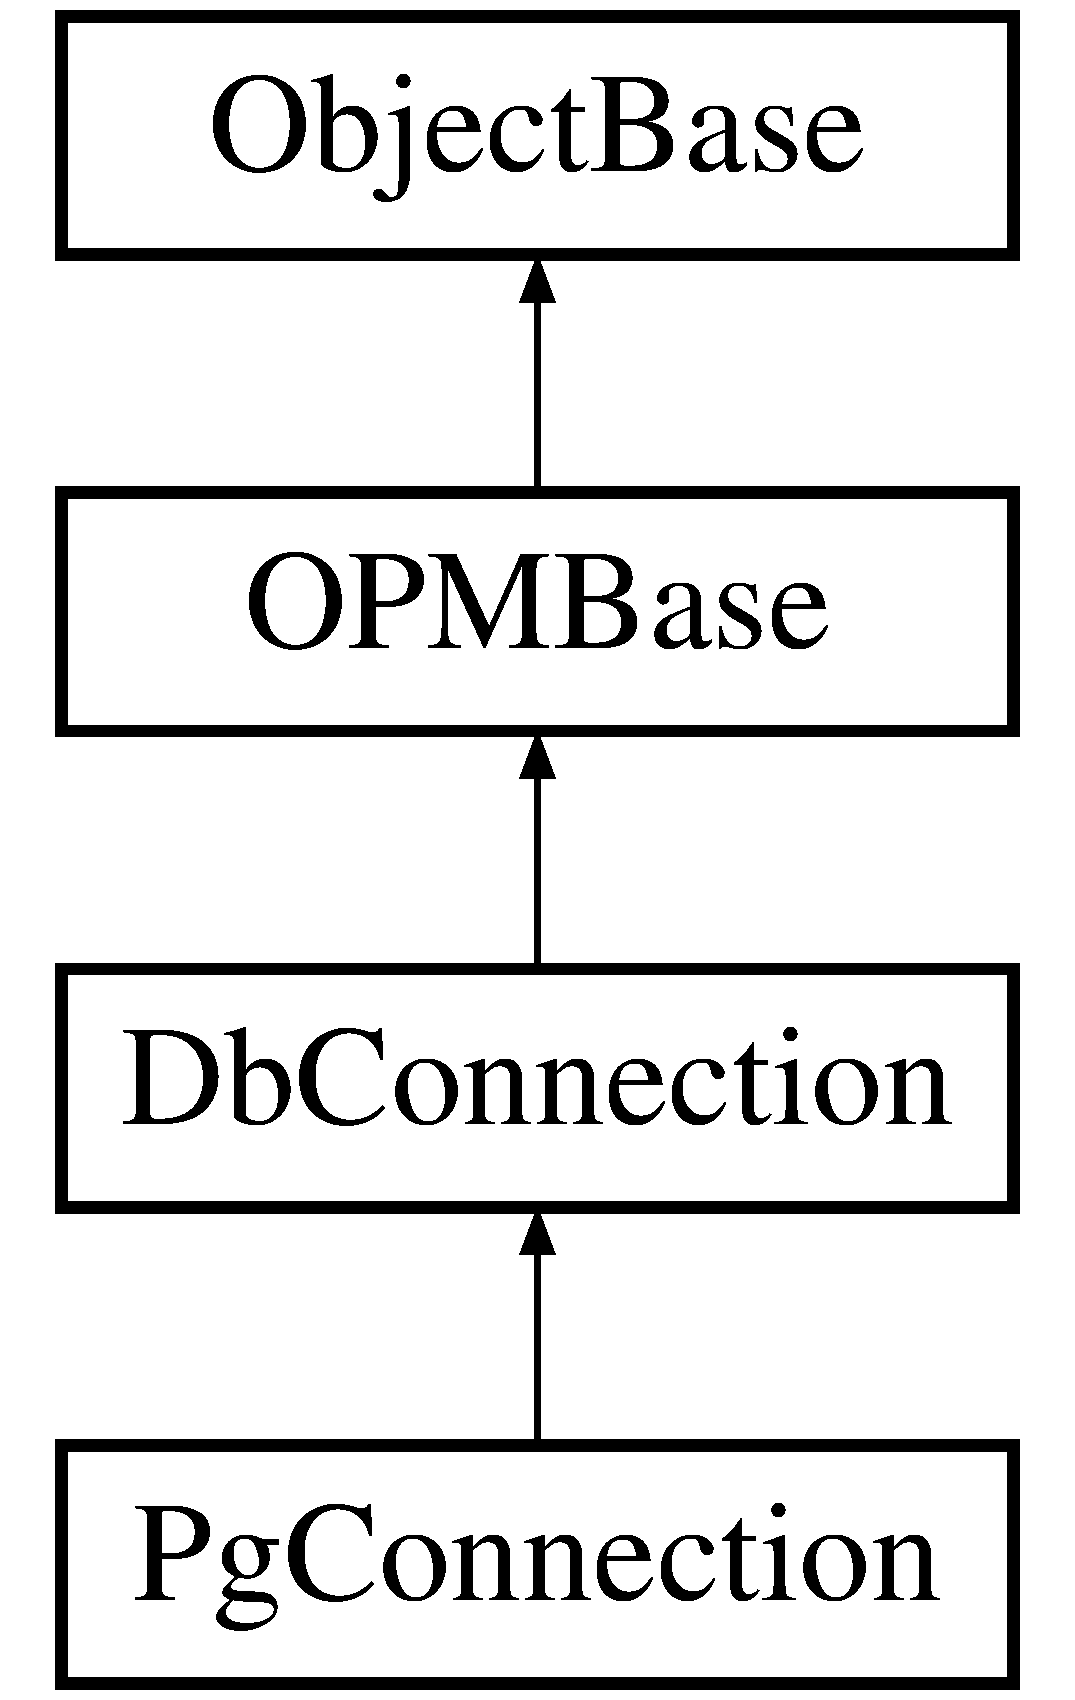
\includegraphics[height=4.000000cm]{classDbConnection}
\end{center}
\end{figure}
\subsection*{Public Member Functions}
\begin{DoxyCompactItemize}
\item 
virtual {\bf $\sim$\+Db\+Connection} ()
\item 
void {\bf add\+User\+Defined\+Identifier} (string \&identifier)
\item 
string \& {\bf get\+User\+Defined\+Identifier} ()
\item 
void {\bf clear\+User\+Defined\+Identifier} ()
\item 
virtual int {\bf check\+Connection\+Health} ()=0
\item 
virtual int {\bf execute\+Command} (string \&command)=0
\item 
virtual int {\bf execute\+Command} (const char $\ast$command)=0
\item 
virtual int {\bf execute\+Command\+With\+Params} (const char $\ast$command, int number\+Params, const char $\ast$const $\ast$param\+Values, const int $\ast$param\+Lengths, const int $\ast$is\+Binary)=0
\item 
virtual int {\bf begin\+Transaction} ()=0
\item 
virtual int {\bf rollback\+Transaction} ()=0
\item 
virtual int {\bf commit\+Transaction} ()=0
\item 
virtual int {\bf initialize\+Prepared\+Command} (const char $\ast$statement\+Name, const char $\ast$sql\+Command, int number\+Params, const Data\+Manager\+Field\+Type $\ast$param\+Type\+Array)=0
\item 
virtual int {\bf execute\+Prepared\+Command} (const char $\ast$statement\+Name, int number\+Params, const char $\ast$const $\ast$param\+Values, const int $\ast$param\+Lengths, const int $\ast$is\+Binary)=0
\item 
virtual int {\bf close\+Command\+Result} ()=0
\item 
virtual int {\bf get\+Column\+Count} ()=0
\item 
virtual string {\bf get\+Column\+Name} (int column\+Index)=0
\item 
virtual int {\bf get\+Column\+Index} (const char $\ast$column\+Name)=0
\item 
virtual int {\bf get\+Row\+Count} ()=0
\item 
virtual const char $\ast$ {\bf get\+String\+Value\+At} (int row\+Index, int column\+Index)=0
\item 
virtual short {\bf get\+Short\+Value\+At} (int row\+Index, int column\+Index)=0
\item 
virtual int {\bf get\+Int\+Value\+At} (int row\+Index, int column\+Index)=0
\item 
virtual bool {\bf get\+Boolean\+Value\+At} (int row\+Index, int column\+Index)=0
\item 
virtual const char $\ast$ {\bf get\+Timestamp\+Value\+At} (int row\+Index, int column\+Index)=0
\item 
virtual bool {\bf is\+Value\+N\+U\+LL} (int row\+Index, int column\+Index)=0
\item 
virtual int {\bf get\+Value\+Length} (int row\+Index, int column\+Index)=0
\item 
virtual void {\bf shutdown} ()=0
\item 
string {\bf to\+String} ()
\end{DoxyCompactItemize}
\subsection*{Protected Member Functions}
\begin{DoxyCompactItemize}
\item 
{\bf Db\+Connection} ()
\end{DoxyCompactItemize}
\subsection*{Additional Inherited Members}


\subsection{Detailed Description}
\doxyref{Db\+Connection}{p.}{classDbConnection} provides an abstract base class for deriving all database-\/specific connection classes from. 

\begin{DoxyParagraph}{Author}
Stephen Horton
\end{DoxyParagraph}
\begin{DoxyParagraph}{Revision}
1
\end{DoxyParagraph}


\subsection{Constructor \& Destructor Documentation}
\index{Db\+Connection@{Db\+Connection}!````~Db\+Connection@{$\sim$\+Db\+Connection}}
\index{````~Db\+Connection@{$\sim$\+Db\+Connection}!Db\+Connection@{Db\+Connection}}
\subsubsection[{$\sim$\+Db\+Connection()}]{\setlength{\rightskip}{0pt plus 5cm}Db\+Connection\+::$\sim$\+Db\+Connection (
\begin{DoxyParamCaption}
{}
\end{DoxyParamCaption}
)\hspace{0.3cm}{\ttfamily [virtual]}}\label{classDbConnection_a643530423c7954f061b8e6f694bfefea}
Virtual Destructor \index{Db\+Connection@{Db\+Connection}!Db\+Connection@{Db\+Connection}}
\index{Db\+Connection@{Db\+Connection}!Db\+Connection@{Db\+Connection}}
\subsubsection[{Db\+Connection()}]{\setlength{\rightskip}{0pt plus 5cm}Db\+Connection\+::\+Db\+Connection (
\begin{DoxyParamCaption}
{}
\end{DoxyParamCaption}
)\hspace{0.3cm}{\ttfamily [protected]}}\label{classDbConnection_a2bb188cd2011a3f8ee580fd34d92422c}
Constructor 

\subsection{Member Function Documentation}
\index{Db\+Connection@{Db\+Connection}!add\+User\+Defined\+Identifier@{add\+User\+Defined\+Identifier}}
\index{add\+User\+Defined\+Identifier@{add\+User\+Defined\+Identifier}!Db\+Connection@{Db\+Connection}}
\subsubsection[{add\+User\+Defined\+Identifier(string \&identifier)}]{\setlength{\rightskip}{0pt plus 5cm}void Db\+Connection\+::add\+User\+Defined\+Identifier (
\begin{DoxyParamCaption}
\item[{string \&}]{identifier}
\end{DoxyParamCaption}
)}\label{classDbConnection_a768c4ae2a92a8dbe12438ca5b4d8acb3}
Allows the Application Developer to \textquotesingle{}tag\textquotesingle{} a particular connection (through this connection handle) with some user-\/defined identification data. This data tag will be preserved even if the connection it checked back into the pool (released) and then reserved again. Thus, the developer can identify which connection was used for which previous tasks. 

Referenced by Db\+Connection\+Handle\+::add\+User\+Defined\+Identifier().

\index{Db\+Connection@{Db\+Connection}!begin\+Transaction@{begin\+Transaction}}
\index{begin\+Transaction@{begin\+Transaction}!Db\+Connection@{Db\+Connection}}
\subsubsection[{begin\+Transaction()=0}]{\setlength{\rightskip}{0pt plus 5cm}virtual int Db\+Connection\+::begin\+Transaction (
\begin{DoxyParamCaption}
{}
\end{DoxyParamCaption}
)\hspace{0.3cm}{\ttfamily [pure virtual]}}\label{classDbConnection_a96c41ce2103f3c8773b85edc87f1a636}
Begin a transaction on this connection. Autocommit is E\+N\+A\+B\+L\+ED for all executed commands U\+N\+L\+E\+SS begin\+Transaction has been called--that is, begin\+Transaction disabled autocommit until either rollback\+Transaction or commit\+Transaction is called. 

Implemented in {\bf Pg\+Connection} \doxyref{}{p.}{classPgConnection_a49a80f8d30f323195087af648982af49}.



Referenced by Db\+Connection\+Handle\+::begin\+Transaction().

\index{Db\+Connection@{Db\+Connection}!check\+Connection\+Health@{check\+Connection\+Health}}
\index{check\+Connection\+Health@{check\+Connection\+Health}!Db\+Connection@{Db\+Connection}}
\subsubsection[{check\+Connection\+Health()=0}]{\setlength{\rightskip}{0pt plus 5cm}virtual int Db\+Connection\+::check\+Connection\+Health (
\begin{DoxyParamCaption}
{}
\end{DoxyParamCaption}
)\hspace{0.3cm}{\ttfamily [pure virtual]}}\label{classDbConnection_a2be956ac44bafb13f437d3896c84caf0}
Check the health of the database connection. \begin{DoxyReturn}{Returns}
OK if the connection is valid; otherwise E\+R\+R\+OR 
\end{DoxyReturn}


Implemented in {\bf Pg\+Connection} \doxyref{}{p.}{classPgConnection_aab4d85a2424a612ff3e7d864d8a7018d}.



Referenced by Db\+Connection\+Handle\+::check\+Connection\+Health().

\index{Db\+Connection@{Db\+Connection}!clear\+User\+Defined\+Identifier@{clear\+User\+Defined\+Identifier}}
\index{clear\+User\+Defined\+Identifier@{clear\+User\+Defined\+Identifier}!Db\+Connection@{Db\+Connection}}
\subsubsection[{clear\+User\+Defined\+Identifier()}]{\setlength{\rightskip}{0pt plus 5cm}void Db\+Connection\+::clear\+User\+Defined\+Identifier (
\begin{DoxyParamCaption}
{}
\end{DoxyParamCaption}
)}\label{classDbConnection_ae0ffda297d8cd846147696675648b79c}
Clears the user-\/defined data and resets the internal string to empty 

Referenced by Db\+Connection\+Handle\+::clear\+User\+Defined\+Identifier().

\index{Db\+Connection@{Db\+Connection}!close\+Command\+Result@{close\+Command\+Result}}
\index{close\+Command\+Result@{close\+Command\+Result}!Db\+Connection@{Db\+Connection}}
\subsubsection[{close\+Command\+Result()=0}]{\setlength{\rightskip}{0pt plus 5cm}virtual int Db\+Connection\+::close\+Command\+Result (
\begin{DoxyParamCaption}
{}
\end{DoxyParamCaption}
)\hspace{0.3cm}{\ttfamily [pure virtual]}}\label{classDbConnection_a5d84f3221afa420916601cb19e65f936}
If an outstanding/open command result\+Set exists for this connection, then close it. 

Implemented in {\bf Pg\+Connection} \doxyref{}{p.}{classPgConnection_ac0564db8f6545b6492cf192fd7540861}.



Referenced by Db\+Connection\+Handle\+::close\+Command\+Result().

\index{Db\+Connection@{Db\+Connection}!commit\+Transaction@{commit\+Transaction}}
\index{commit\+Transaction@{commit\+Transaction}!Db\+Connection@{Db\+Connection}}
\subsubsection[{commit\+Transaction()=0}]{\setlength{\rightskip}{0pt plus 5cm}virtual int Db\+Connection\+::commit\+Transaction (
\begin{DoxyParamCaption}
{}
\end{DoxyParamCaption}
)\hspace{0.3cm}{\ttfamily [pure virtual]}}\label{classDbConnection_a52920fd2ac90fa63fc3b12f2ba5df119}
Commit the outstanding transaction on this connection 

Implemented in {\bf Pg\+Connection} \doxyref{}{p.}{classPgConnection_a84e5a33c996614e08eaff923e2b0b12c}.



Referenced by Db\+Connection\+Handle\+::commit\+Transaction().

\index{Db\+Connection@{Db\+Connection}!execute\+Command@{execute\+Command}}
\index{execute\+Command@{execute\+Command}!Db\+Connection@{Db\+Connection}}
\subsubsection[{execute\+Command(string \&command)=0}]{\setlength{\rightskip}{0pt plus 5cm}virtual int Db\+Connection\+::execute\+Command (
\begin{DoxyParamCaption}
\item[{string \&}]{command}
\end{DoxyParamCaption}
)\hspace{0.3cm}{\ttfamily [pure virtual]}}\label{classDbConnection_a83651597d0bfd2f7a20e5305502e207f}
Execute an S\+QL command to the database using this connection. This command can be a Q\+U\+E\+RY, U\+P\+D\+A\+TE, I\+N\+S\+E\+RT, or D\+E\+L\+E\+TE operation. \begin{DoxyReturn}{Returns}
OK if the command was executed successfully; otherwise E\+R\+R\+OR 
\end{DoxyReturn}


Implemented in {\bf Pg\+Connection} \doxyref{}{p.}{classPgConnection_a7552b483ef7fea3220ea545522195c44}.



Referenced by Db\+Connection\+Handle\+::execute\+Command().

\index{Db\+Connection@{Db\+Connection}!execute\+Command@{execute\+Command}}
\index{execute\+Command@{execute\+Command}!Db\+Connection@{Db\+Connection}}
\subsubsection[{execute\+Command(const char $\ast$command)=0}]{\setlength{\rightskip}{0pt plus 5cm}virtual int Db\+Connection\+::execute\+Command (
\begin{DoxyParamCaption}
\item[{const char $\ast$}]{command}
\end{DoxyParamCaption}
)\hspace{0.3cm}{\ttfamily [pure virtual]}}\label{classDbConnection_a27631d58f737d2476b39e17ea16804d0}
Execute an S\+QL command to the database using this connection. This command can be a Q\+U\+E\+RY, U\+P\+D\+A\+TE, I\+N\+S\+E\+RT, or D\+E\+L\+E\+TE operation. (To work with ostringstream) \begin{DoxyReturn}{Returns}
OK if the command was executed successfully; otherwise E\+R\+R\+OR 
\end{DoxyReturn}


Implemented in {\bf Pg\+Connection} \doxyref{}{p.}{classPgConnection_aa91f5ba0537b074769cf3c864d407e63}.

\index{Db\+Connection@{Db\+Connection}!execute\+Command\+With\+Params@{execute\+Command\+With\+Params}}
\index{execute\+Command\+With\+Params@{execute\+Command\+With\+Params}!Db\+Connection@{Db\+Connection}}
\subsubsection[{execute\+Command\+With\+Params(const char $\ast$command, int number\+Params, const char $\ast$const $\ast$param\+Values, const int $\ast$param\+Lengths, const int $\ast$is\+Binary)=0}]{\setlength{\rightskip}{0pt plus 5cm}virtual int Db\+Connection\+::execute\+Command\+With\+Params (
\begin{DoxyParamCaption}
\item[{const char $\ast$}]{command, }
\item[{int}]{number\+Params, }
\item[{const char $\ast$const $\ast$}]{param\+Values, }
\item[{const int $\ast$}]{param\+Lengths, }
\item[{const int $\ast$}]{is\+Binary}
\end{DoxyParamCaption}
)\hspace{0.3cm}{\ttfamily [pure virtual]}}\label{classDbConnection_a28e07e7dc5d986fa2135c3e0ecab19b2}
Execute an S\+QL command to the database using this connection. This command can be a Q\+U\+E\+RY, U\+P\+D\+A\+TE, I\+N\+S\+E\+RT or D\+E\+L\+E\+TE operation. 
\begin{DoxyParams}{Parameters}
{\em number\+Params} & number of passed in parameters in the char$\ast$ array \\
\hline
{\em param\+Values} & specifies the actual values of the parameters (char$\ast$ array) \\
\hline
{\em param\+Lengths} & specifies the actual data lengths of binary-\/format parameters. It is ignored for null parameters and text-\/format parameters. The array pointer may be null when there are no binary parameters. \\
\hline
{\em is\+Binary} & array for each param value to determine if the value is binary or textual (T\+R\+UE for binary / F\+A\+L\+SE for text). The array pointer may be null when there are no binary parameters. \\
\hline
\end{DoxyParams}
\begin{DoxyReturn}{Returns}
OK if the command was executed successfully; otherwise E\+R\+R\+OR 
\end{DoxyReturn}


Implemented in {\bf Pg\+Connection} \doxyref{}{p.}{classPgConnection_a48fbb1b1e44e9f93cd900937f7f54ea8}.



Referenced by Db\+Connection\+Handle\+::execute\+Command\+With\+Params().

\index{Db\+Connection@{Db\+Connection}!execute\+Prepared\+Command@{execute\+Prepared\+Command}}
\index{execute\+Prepared\+Command@{execute\+Prepared\+Command}!Db\+Connection@{Db\+Connection}}
\subsubsection[{execute\+Prepared\+Command(const char $\ast$statement\+Name, int number\+Params, const char $\ast$const $\ast$param\+Values, const int $\ast$param\+Lengths, const int $\ast$is\+Binary)=0}]{\setlength{\rightskip}{0pt plus 5cm}virtual int Db\+Connection\+::execute\+Prepared\+Command (
\begin{DoxyParamCaption}
\item[{const char $\ast$}]{statement\+Name, }
\item[{int}]{number\+Params, }
\item[{const char $\ast$const $\ast$}]{param\+Values, }
\item[{const int $\ast$}]{param\+Lengths, }
\item[{const int $\ast$}]{is\+Binary}
\end{DoxyParamCaption}
)\hspace{0.3cm}{\ttfamily [pure virtual]}}\label{classDbConnection_a53ac83159ba5d2548465c4318e6e5d85}
Execute an S\+QL prepared statement command to the database using this connection. This command can be a Q\+U\+E\+RY, U\+P\+D\+A\+TE, I\+N\+S\+E\+RT, or D\+E\+L\+E\+TE operation. 
\begin{DoxyParams}{Parameters}
{\em statement\+Name} & string name assigned to the statement when initialize\+Prepared\+Command is called. \\
\hline
{\em number\+Params} & number of passed in parameters in the char$\ast$ array \\
\hline
{\em param\+Values} & specifies the actual values of the parameters (char$\ast$ array) \\
\hline
{\em param\+Lengths} & specifies the actual data lengths of binary-\/format parameters. It is ignored for null parameters and text-\/format parameters. The array pointer may be null when there are no binary parameters. \\
\hline
{\em is\+Binary} & array for each param value to determine if the value is binary or textual (T\+R\+UE for binary / F\+A\+L\+SE for text). The array pointer may be null when there are no binary parameters. \\
\hline
\end{DoxyParams}
\begin{DoxyReturn}{Returns}
OK if the command was successfully executed; otherwise E\+R\+R\+OR 
\end{DoxyReturn}


Implemented in {\bf Pg\+Connection} \doxyref{}{p.}{classPgConnection_a99fabc4a40f6bf2aa87cf35ef07e3d2c}.



Referenced by Db\+Connection\+Handle\+::execute\+Prepared\+Command().

\index{Db\+Connection@{Db\+Connection}!get\+Boolean\+Value\+At@{get\+Boolean\+Value\+At}}
\index{get\+Boolean\+Value\+At@{get\+Boolean\+Value\+At}!Db\+Connection@{Db\+Connection}}
\subsubsection[{get\+Boolean\+Value\+At(int row\+Index, int column\+Index)=0}]{\setlength{\rightskip}{0pt plus 5cm}virtual bool Db\+Connection\+::get\+Boolean\+Value\+At (
\begin{DoxyParamCaption}
\item[{int}]{row\+Index, }
\item[{int}]{column\+Index}
\end{DoxyParamCaption}
)\hspace{0.3cm}{\ttfamily [pure virtual]}}\label{classDbConnection_a47d76e5c335cf87a51b4ae799142853b}
Return the value at the specified column/row location in the current command\+Result. The value returned will be a boolean type. N\+O\+TE\+: Use of this method requires that the developer be aware of the of the schema and result field type. 

Implemented in {\bf Pg\+Connection} \doxyref{}{p.}{classPgConnection_a79f7bc4f806ef47b29d2a35f4a15a3a2}.



Referenced by Db\+Connection\+Handle\+::get\+Boolean\+Value\+At().

\index{Db\+Connection@{Db\+Connection}!get\+Column\+Count@{get\+Column\+Count}}
\index{get\+Column\+Count@{get\+Column\+Count}!Db\+Connection@{Db\+Connection}}
\subsubsection[{get\+Column\+Count()=0}]{\setlength{\rightskip}{0pt plus 5cm}virtual int Db\+Connection\+::get\+Column\+Count (
\begin{DoxyParamCaption}
{}
\end{DoxyParamCaption}
)\hspace{0.3cm}{\ttfamily [pure virtual]}}\label{classDbConnection_a009d7e80ce19a8f1d8b2e1de9fee0215}
Return the number of columns in the current command\+Result structure 

Implemented in {\bf Pg\+Connection} \doxyref{}{p.}{classPgConnection_a3630587032d9168e3cd18e3079013311}.



Referenced by Db\+Connection\+Handle\+::get\+Column\+Count().

\index{Db\+Connection@{Db\+Connection}!get\+Column\+Index@{get\+Column\+Index}}
\index{get\+Column\+Index@{get\+Column\+Index}!Db\+Connection@{Db\+Connection}}
\subsubsection[{get\+Column\+Index(const char $\ast$column\+Name)=0}]{\setlength{\rightskip}{0pt plus 5cm}virtual int Db\+Connection\+::get\+Column\+Index (
\begin{DoxyParamCaption}
\item[{const char $\ast$}]{column\+Name}
\end{DoxyParamCaption}
)\hspace{0.3cm}{\ttfamily [pure virtual]}}\label{classDbConnection_a14e5da7507568c814674659d95d3bc7d}
Return the column index based on the specified column name 

Implemented in {\bf Pg\+Connection} \doxyref{}{p.}{classPgConnection_addaa8aab285b4e62ed1d7028fa4537f0}.



Referenced by Db\+Connection\+Handle\+::get\+Column\+Index().

\index{Db\+Connection@{Db\+Connection}!get\+Column\+Name@{get\+Column\+Name}}
\index{get\+Column\+Name@{get\+Column\+Name}!Db\+Connection@{Db\+Connection}}
\subsubsection[{get\+Column\+Name(int column\+Index)=0}]{\setlength{\rightskip}{0pt plus 5cm}virtual string Db\+Connection\+::get\+Column\+Name (
\begin{DoxyParamCaption}
\item[{int}]{column\+Index}
\end{DoxyParamCaption}
)\hspace{0.3cm}{\ttfamily [pure virtual]}}\label{classDbConnection_acd94d1646175616a059e49be0bf6dcc8}
Return the specified column header name in the current command\+Result 

Implemented in {\bf Pg\+Connection} \doxyref{}{p.}{classPgConnection_a947a3e65e61ec47a9fb1261448733576}.



Referenced by Db\+Connection\+Handle\+::get\+Column\+Name().

\index{Db\+Connection@{Db\+Connection}!get\+Int\+Value\+At@{get\+Int\+Value\+At}}
\index{get\+Int\+Value\+At@{get\+Int\+Value\+At}!Db\+Connection@{Db\+Connection}}
\subsubsection[{get\+Int\+Value\+At(int row\+Index, int column\+Index)=0}]{\setlength{\rightskip}{0pt plus 5cm}virtual int Db\+Connection\+::get\+Int\+Value\+At (
\begin{DoxyParamCaption}
\item[{int}]{row\+Index, }
\item[{int}]{column\+Index}
\end{DoxyParamCaption}
)\hspace{0.3cm}{\ttfamily [pure virtual]}}\label{classDbConnection_a71ad6f31c85f225087f20ae8f074f309}
Return the value at the specified column/row location in the current command\+Result. The value returned will be a 4-\/byte integer type. N\+O\+TE\+: Use of this method requires that the developer be aware of the of the schema and result field type. 

Implemented in {\bf Pg\+Connection} \doxyref{}{p.}{classPgConnection_a8f86b49b4ef4ced8a482b72b16a39a10}.



Referenced by Db\+Connection\+Handle\+::get\+Int\+Value\+At().

\index{Db\+Connection@{Db\+Connection}!get\+Row\+Count@{get\+Row\+Count}}
\index{get\+Row\+Count@{get\+Row\+Count}!Db\+Connection@{Db\+Connection}}
\subsubsection[{get\+Row\+Count()=0}]{\setlength{\rightskip}{0pt plus 5cm}virtual int Db\+Connection\+::get\+Row\+Count (
\begin{DoxyParamCaption}
{}
\end{DoxyParamCaption}
)\hspace{0.3cm}{\ttfamily [pure virtual]}}\label{classDbConnection_a43a2add9e2a787e1576948d374789a1f}
Return the number of rows in the current command\+Result 

Implemented in {\bf Pg\+Connection} \doxyref{}{p.}{classPgConnection_a2009e9b9cdb3654da5c05fd1961f4563}.



Referenced by Db\+Connection\+Handle\+::get\+Row\+Count().

\index{Db\+Connection@{Db\+Connection}!get\+Short\+Value\+At@{get\+Short\+Value\+At}}
\index{get\+Short\+Value\+At@{get\+Short\+Value\+At}!Db\+Connection@{Db\+Connection}}
\subsubsection[{get\+Short\+Value\+At(int row\+Index, int column\+Index)=0}]{\setlength{\rightskip}{0pt plus 5cm}virtual short Db\+Connection\+::get\+Short\+Value\+At (
\begin{DoxyParamCaption}
\item[{int}]{row\+Index, }
\item[{int}]{column\+Index}
\end{DoxyParamCaption}
)\hspace{0.3cm}{\ttfamily [pure virtual]}}\label{classDbConnection_a8b070bdb24663b7532fb8d87d249bfba}
Return the value at the specified column/row location in the current command\+Result. The value returned will be a 2-\/byte short type. N\+O\+TE\+: Use of this method requires that the developer be aware of the of the schema and result field type. 

Implemented in {\bf Pg\+Connection} \doxyref{}{p.}{classPgConnection_ad2ec4474be2fe45aac4091bcf2c5cd22}.



Referenced by Db\+Connection\+Handle\+::get\+Short\+Value\+At().

\index{Db\+Connection@{Db\+Connection}!get\+String\+Value\+At@{get\+String\+Value\+At}}
\index{get\+String\+Value\+At@{get\+String\+Value\+At}!Db\+Connection@{Db\+Connection}}
\subsubsection[{get\+String\+Value\+At(int row\+Index, int column\+Index)=0}]{\setlength{\rightskip}{0pt plus 5cm}virtual const char$\ast$ Db\+Connection\+::get\+String\+Value\+At (
\begin{DoxyParamCaption}
\item[{int}]{row\+Index, }
\item[{int}]{column\+Index}
\end{DoxyParamCaption}
)\hspace{0.3cm}{\ttfamily [pure virtual]}}\label{classDbConnection_abf8cdacfc76d7d593810aaba97bc1e4a}
Return the value at the specified column/row location in the current command\+Result. The value is returned as a string. N\+O\+TE\+: Use of this method requires that the developer be aware of the of the schema and result field type. 

Implemented in {\bf Pg\+Connection} \doxyref{}{p.}{classPgConnection_abb7d95bb6b406abb81cf442f8cbb4aab}.



Referenced by Db\+Connection\+Handle\+::get\+String\+Value\+At().

\index{Db\+Connection@{Db\+Connection}!get\+Timestamp\+Value\+At@{get\+Timestamp\+Value\+At}}
\index{get\+Timestamp\+Value\+At@{get\+Timestamp\+Value\+At}!Db\+Connection@{Db\+Connection}}
\subsubsection[{get\+Timestamp\+Value\+At(int row\+Index, int column\+Index)=0}]{\setlength{\rightskip}{0pt plus 5cm}virtual const char$\ast$ Db\+Connection\+::get\+Timestamp\+Value\+At (
\begin{DoxyParamCaption}
\item[{int}]{row\+Index, }
\item[{int}]{column\+Index}
\end{DoxyParamCaption}
)\hspace{0.3cm}{\ttfamily [pure virtual]}}\label{classDbConnection_a012b6ab3732da18176d52ee1ee02581c}
Return the value at the specified column/row location in the current command\+Result. The value returned will be a string. N\+O\+TE\+: Use of this method requires that the developer be aware of the of the schema and result field type. 

Implemented in {\bf Pg\+Connection} \doxyref{}{p.}{classPgConnection_ae434771a41f3c44c5a1d7a1cbbc24514}.



Referenced by Db\+Connection\+Handle\+::get\+Timestamp\+Value\+At().

\index{Db\+Connection@{Db\+Connection}!get\+User\+Defined\+Identifier@{get\+User\+Defined\+Identifier}}
\index{get\+User\+Defined\+Identifier@{get\+User\+Defined\+Identifier}!Db\+Connection@{Db\+Connection}}
\subsubsection[{get\+User\+Defined\+Identifier()}]{\setlength{\rightskip}{0pt plus 5cm}string \& Db\+Connection\+::get\+User\+Defined\+Identifier (
\begin{DoxyParamCaption}
{}
\end{DoxyParamCaption}
)}\label{classDbConnection_a3f4142844f6237fb93cdd68bab72422d}
Returns the user-\/defined identifier data \begin{DoxyReturn}{Returns}
empty string if no user-\/defined data has been previously set 
\end{DoxyReturn}


Referenced by Db\+Connection\+Handle\+::get\+User\+Defined\+Identifier().

\index{Db\+Connection@{Db\+Connection}!get\+Value\+Length@{get\+Value\+Length}}
\index{get\+Value\+Length@{get\+Value\+Length}!Db\+Connection@{Db\+Connection}}
\subsubsection[{get\+Value\+Length(int row\+Index, int column\+Index)=0}]{\setlength{\rightskip}{0pt plus 5cm}virtual int Db\+Connection\+::get\+Value\+Length (
\begin{DoxyParamCaption}
\item[{int}]{row\+Index, }
\item[{int}]{column\+Index}
\end{DoxyParamCaption}
)\hspace{0.3cm}{\ttfamily [pure virtual]}}\label{classDbConnection_a972e54509577bf23dbc82be7727cf355}
Returns the actual length of a field value in bytes 

Implemented in {\bf Pg\+Connection} \doxyref{}{p.}{classPgConnection_aa6132f27beb7c695a524747115be1573}.



Referenced by Db\+Connection\+Handle\+::get\+Value\+Length().

\index{Db\+Connection@{Db\+Connection}!initialize\+Prepared\+Command@{initialize\+Prepared\+Command}}
\index{initialize\+Prepared\+Command@{initialize\+Prepared\+Command}!Db\+Connection@{Db\+Connection}}
\subsubsection[{initialize\+Prepared\+Command(const char $\ast$statement\+Name, const char $\ast$sql\+Command, int number\+Params, const Data\+Manager\+Field\+Type $\ast$param\+Type\+Array)=0}]{\setlength{\rightskip}{0pt plus 5cm}virtual int Db\+Connection\+::initialize\+Prepared\+Command (
\begin{DoxyParamCaption}
\item[{const char $\ast$}]{statement\+Name, }
\item[{const char $\ast$}]{sql\+Command, }
\item[{int}]{number\+Params, }
\item[{const Data\+Manager\+Field\+Type $\ast$}]{param\+Type\+Array}
\end{DoxyParamCaption}
)\hspace{0.3cm}{\ttfamily [pure virtual]}}\label{classDbConnection_ac4f42fcce6c8a088f7e38735a7dbb202}
Setup for a prepared statement command on this connection 
\begin{DoxyParams}{Parameters}
{\em statement\+Name} & string name arbitrarily assigned to the statement \\
\hline
{\em sql\+Command} & Q\+U\+E\+RY, U\+P\+D\+A\+TE, I\+N\+S\+E\+RT, or D\+E\+L\+E\+TE sql operation. \\
\hline
{\em number\+Params} & number of passed in parameters in the char$\ast$ array \\
\hline
{\em param\+Type\+Array} & array of field types because the database cannot infer the field type formatting without it. \\
\hline
\end{DoxyParams}
\begin{DoxyReturn}{Returns}
OK if the preparation was successful; otherwise E\+R\+R\+OR 
\end{DoxyReturn}


Implemented in {\bf Pg\+Connection} \doxyref{}{p.}{classPgConnection_aecfbf962ca0b92c5b4208f9baf5ac098}.



Referenced by Db\+Connection\+Handle\+::initialize\+Prepared\+Command().

\index{Db\+Connection@{Db\+Connection}!is\+Value\+N\+U\+LL@{is\+Value\+N\+U\+LL}}
\index{is\+Value\+N\+U\+LL@{is\+Value\+N\+U\+LL}!Db\+Connection@{Db\+Connection}}
\subsubsection[{is\+Value\+N\+U\+L\+L(int row\+Index, int column\+Index)=0}]{\setlength{\rightskip}{0pt plus 5cm}virtual bool Db\+Connection\+::is\+Value\+N\+U\+LL (
\begin{DoxyParamCaption}
\item[{int}]{row\+Index, }
\item[{int}]{column\+Index}
\end{DoxyParamCaption}
)\hspace{0.3cm}{\ttfamily [pure virtual]}}\label{classDbConnection_a4f8a595206996b804c7fbb2a8c4c51a7}
Returns true if the field Value is N\+U\+LL 

Implemented in {\bf Pg\+Connection} \doxyref{}{p.}{classPgConnection_a5dc5867034b6a73ecd9cf379e5e21f70}.



Referenced by Db\+Connection\+Handle\+::is\+Value\+N\+U\+L\+L().

\index{Db\+Connection@{Db\+Connection}!rollback\+Transaction@{rollback\+Transaction}}
\index{rollback\+Transaction@{rollback\+Transaction}!Db\+Connection@{Db\+Connection}}
\subsubsection[{rollback\+Transaction()=0}]{\setlength{\rightskip}{0pt plus 5cm}virtual int Db\+Connection\+::rollback\+Transaction (
\begin{DoxyParamCaption}
{}
\end{DoxyParamCaption}
)\hspace{0.3cm}{\ttfamily [pure virtual]}}\label{classDbConnection_a8133c5c71e712d374ff0d8ce8a4447ca}
Rollback a transaction on this connection 

Implemented in {\bf Pg\+Connection} \doxyref{}{p.}{classPgConnection_a808492b9837316f2a3fe48de894a1e69}.



Referenced by Db\+Connection\+Handle\+::rollback\+Transaction().

\index{Db\+Connection@{Db\+Connection}!shutdown@{shutdown}}
\index{shutdown@{shutdown}!Db\+Connection@{Db\+Connection}}
\subsubsection[{shutdown()=0}]{\setlength{\rightskip}{0pt plus 5cm}virtual void Db\+Connection\+::shutdown (
\begin{DoxyParamCaption}
{}
\end{DoxyParamCaption}
)\hspace{0.3cm}{\ttfamily [pure virtual]}}\label{classDbConnection_a4e978e217bda3f0bcbe8ffb505525649}
Close the socket connection to the database server 

Implemented in {\bf Pg\+Connection} \doxyref{}{p.}{classPgConnection_aca1ac3e68950124dd743e7b87428d147}.



Referenced by Db\+Connection\+Handle\+::shutdown().

\index{Db\+Connection@{Db\+Connection}!to\+String@{to\+String}}
\index{to\+String@{to\+String}!Db\+Connection@{Db\+Connection}}
\subsubsection[{to\+String()}]{\setlength{\rightskip}{0pt plus 5cm}string Db\+Connection\+::to\+String (
\begin{DoxyParamCaption}
{}
\end{DoxyParamCaption}
)}\label{classDbConnection_ae4cd401b4f590d8d5fec71afd1ec4e36}
String\textquotesingle{}ized debugging method \begin{DoxyReturn}{Returns}
string representation of the contents of this object 
\end{DoxyReturn}


The documentation for this class was generated from the following files\+:\begin{DoxyCompactItemize}
\item 
Db\+Connection.\+h\item 
Db\+Connection.\+cpp\end{DoxyCompactItemize}

\section{Db\+Connection\+Handle Class Reference}
\label{classDbConnectionHandle}\index{Db\+Connection\+Handle@{Db\+Connection\+Handle}}


{\ttfamily \#include $<$Db\+Connection\+Handle.\+h$>$}

Inheritance diagram for Db\+Connection\+Handle\+:\begin{figure}[H]
\begin{center}
\leavevmode
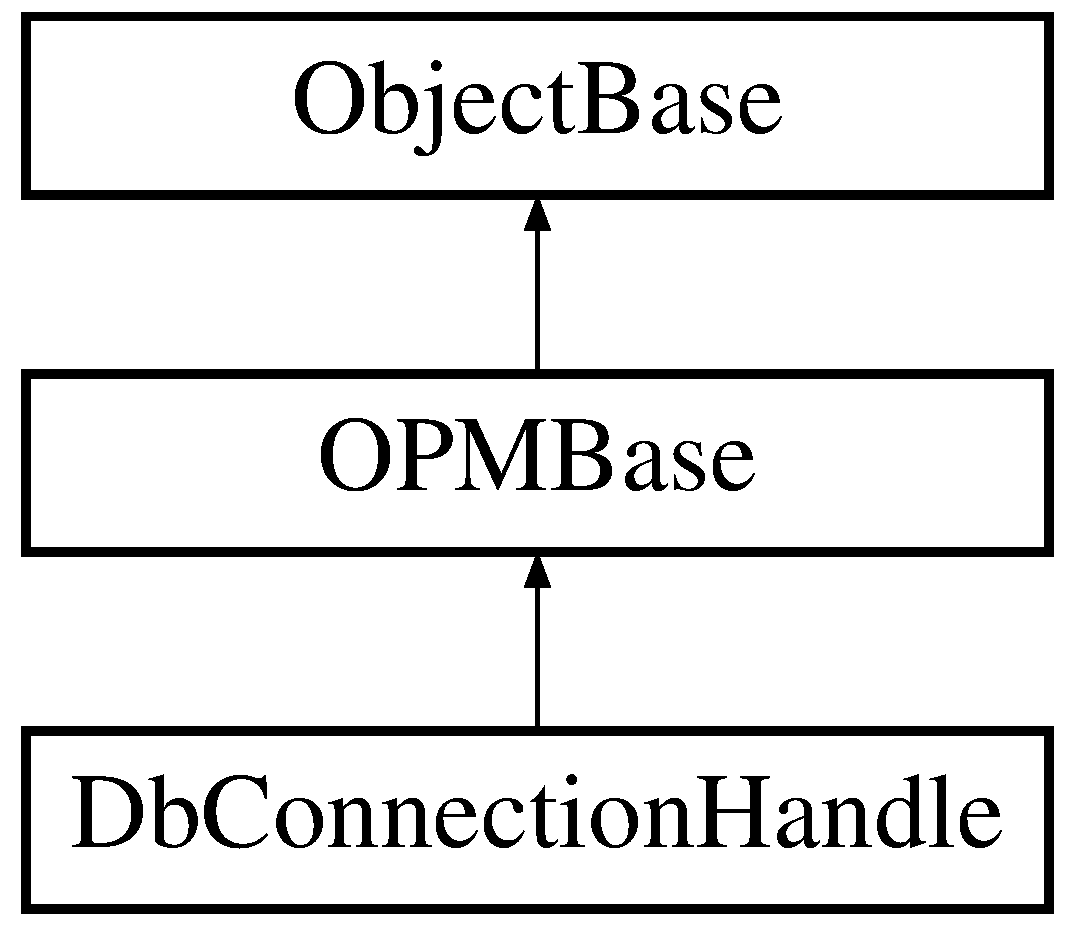
\includegraphics[height=3.000000cm]{classDbConnectionHandle}
\end{center}
\end{figure}
\subsection*{Public Member Functions}
\begin{DoxyCompactItemize}
\item 
{\bf Db\+Connection\+Handle} ()
\item 
virtual {\bf $\sim$\+Db\+Connection\+Handle} ()
\item 
void {\bf clean} ()
\item 
void {\bf add\+User\+Defined\+Identifier} (string \&identifier)
\item 
string \& {\bf get\+User\+Defined\+Identifier} ()
\item 
void {\bf clear\+User\+Defined\+Identifier} ()
\item 
int {\bf check\+Connection\+Health} ()
\item 
int {\bf execute\+Command} (string \&command)
\item 
int {\bf execute\+Command} (const char $\ast$command)
\item 
int {\bf execute\+Command\+With\+Params} (const char $\ast$command, int number\+Params, const char $\ast$const $\ast$param\+Values, const int $\ast$param\+Lengths, const int $\ast$is\+Binary)
\item 
int {\bf begin\+Transaction} ()
\item 
int {\bf rollback\+Transaction} ()
\item 
int {\bf commit\+Transaction} ()
\item 
int {\bf initialize\+Prepared\+Command} (const char $\ast$statement\+Name, const char $\ast$sql\+Command, int number\+Params, const Data\+Manager\+Field\+Type $\ast$param\+Type\+Array)
\item 
int {\bf execute\+Prepared\+Command} (const char $\ast$statement\+Name, int number\+Params, const char $\ast$const $\ast$param\+Values, const int $\ast$param\+Lengths, const int $\ast$is\+Binary)
\item 
int {\bf close\+Command\+Result} ()
\item 
int {\bf get\+Column\+Count} ()
\item 
string {\bf get\+Column\+Name} (int column\+Index)
\item 
int {\bf get\+Column\+Index} (const char $\ast$column\+Name)
\item 
int {\bf get\+Row\+Count} ()
\item 
string {\bf get\+String\+Value\+At} (int row\+Index, int column\+Index)
\item 
short {\bf get\+Short\+Value\+At} (int row\+Index, int column\+Index)
\item 
int {\bf get\+Int\+Value\+At} (int row\+Index, int column\+Index)
\item 
bool {\bf get\+Boolean\+Value\+At} (int row\+Index, int column\+Index)
\item 
string {\bf get\+Timestamp\+Value\+At} (int row\+Index, int column\+Index)
\item 
bool {\bf is\+Value\+N\+U\+LL} (int row\+Index, int column\+Index)
\item 
int {\bf get\+Value\+Length} (int row\+Index, int column\+Index)
\item 
int {\bf shutdown} ()
\item 
string {\bf to\+String} ()
\end{DoxyCompactItemize}
\subsection*{Static Public Member Functions}
\begin{DoxyCompactItemize}
\item 
static {\bf O\+P\+M\+Base} $\ast$ {\bf initialize} (int initializer)
\end{DoxyCompactItemize}
\subsection*{Friends}
\begin{DoxyCompactItemize}
\item 
class {\bf Data\+Manager}
\item 
class {\bf Connection\+Set}
\end{DoxyCompactItemize}
\subsection*{Additional Inherited Members}


\subsection{Detailed Description}
\doxyref{Db\+Connection\+Handle}{p.}{classDbConnectionHandle} class provides a wrapper around the \textquotesingle{}real\textquotesingle{} \doxyref{Db\+Connection}{p.}{classDbConnection} object. 

The strategy here is to prevent the application designer user from gaining access to the \doxyref{Db\+Connection}{p.}{classDbConnection} object and doing something they shouldn\textquotesingle{}t. 

Additionally, \doxyref{Db\+Connection\+Handle}{p.}{classDbConnectionHandle} stores the Thread Id of the thread that reserved the connection. For each operation, it checks to see if the thread that is performing the operation is the same thread that reserved the connection. If it is determined to be different, this can indicate that the application is using a stale pointer to a connection that has already been release back into the pool. The database driver A\+PI is \textquotesingle{}mostly\textquotesingle{} thread safe. However, the architecture of the driver is such that it is intended for use by a single thread--this means that once a query has been performed on the connection and the result set has been returned to the client side via the connection, another query should not be issued until the result set has been completely analyzed (all processing on it complete), and the result set has been closed. 

\begin{DoxyParagraph}{Author}
Stephen Horton
\end{DoxyParagraph}
\begin{DoxyParagraph}{Revision}
1
\end{DoxyParagraph}


\subsection{Constructor \& Destructor Documentation}
\index{Db\+Connection\+Handle@{Db\+Connection\+Handle}!Db\+Connection\+Handle@{Db\+Connection\+Handle}}
\index{Db\+Connection\+Handle@{Db\+Connection\+Handle}!Db\+Connection\+Handle@{Db\+Connection\+Handle}}
\subsubsection[{Db\+Connection\+Handle()}]{\setlength{\rightskip}{0pt plus 5cm}Db\+Connection\+Handle\+::\+Db\+Connection\+Handle (
\begin{DoxyParamCaption}
{}
\end{DoxyParamCaption}
)}\label{classDbConnectionHandle_a6cf5354f0ff51fda04d0dc7de3c3e2b0}
Constructor 

Referenced by initialize().

\index{Db\+Connection\+Handle@{Db\+Connection\+Handle}!````~Db\+Connection\+Handle@{$\sim$\+Db\+Connection\+Handle}}
\index{````~Db\+Connection\+Handle@{$\sim$\+Db\+Connection\+Handle}!Db\+Connection\+Handle@{Db\+Connection\+Handle}}
\subsubsection[{$\sim$\+Db\+Connection\+Handle()}]{\setlength{\rightskip}{0pt plus 5cm}Db\+Connection\+Handle\+::$\sim$\+Db\+Connection\+Handle (
\begin{DoxyParamCaption}
{}
\end{DoxyParamCaption}
)\hspace{0.3cm}{\ttfamily [virtual]}}\label{classDbConnectionHandle_a390e7a702e8313bfc01d330fed193b9d}
Virtual Destructor 

\subsection{Member Function Documentation}
\index{Db\+Connection\+Handle@{Db\+Connection\+Handle}!add\+User\+Defined\+Identifier@{add\+User\+Defined\+Identifier}}
\index{add\+User\+Defined\+Identifier@{add\+User\+Defined\+Identifier}!Db\+Connection\+Handle@{Db\+Connection\+Handle}}
\subsubsection[{add\+User\+Defined\+Identifier(string \&identifier)}]{\setlength{\rightskip}{0pt plus 5cm}void Db\+Connection\+Handle\+::add\+User\+Defined\+Identifier (
\begin{DoxyParamCaption}
\item[{string \&}]{identifier}
\end{DoxyParamCaption}
)}\label{classDbConnectionHandle_ad8d6ae3532c654e29a9770f40b6dde65}
Allows the Application Developer to \textquotesingle{}tag\textquotesingle{} a particular connection (through this connection handle) with some user-\/defined identification data. This data tag will be preserved even if the connection it checked back into the pool (released) and then reserved again. Thus, the developer can identify which connection was used for which previous tasks. 

References Db\+Connection\+::add\+User\+Defined\+Identifier().

\index{Db\+Connection\+Handle@{Db\+Connection\+Handle}!begin\+Transaction@{begin\+Transaction}}
\index{begin\+Transaction@{begin\+Transaction}!Db\+Connection\+Handle@{Db\+Connection\+Handle}}
\subsubsection[{begin\+Transaction()}]{\setlength{\rightskip}{0pt plus 5cm}int Db\+Connection\+Handle\+::begin\+Transaction (
\begin{DoxyParamCaption}
{}
\end{DoxyParamCaption}
)}\label{classDbConnectionHandle_a0ef591e3444061af21da1a19dd18cf6e}
Begin a transaction on this connection. Autocommit is E\+N\+A\+B\+L\+ED for all executed commands U\+N\+L\+E\+SS begin\+Transaction has been called--that is, begin\+Transaction disabled autocommit until either rollback\+Transaction or commit\+Transaction is called. 

References Db\+Connection\+::begin\+Transaction().

\index{Db\+Connection\+Handle@{Db\+Connection\+Handle}!check\+Connection\+Health@{check\+Connection\+Health}}
\index{check\+Connection\+Health@{check\+Connection\+Health}!Db\+Connection\+Handle@{Db\+Connection\+Handle}}
\subsubsection[{check\+Connection\+Health()}]{\setlength{\rightskip}{0pt plus 5cm}int Db\+Connection\+Handle\+::check\+Connection\+Health (
\begin{DoxyParamCaption}
{}
\end{DoxyParamCaption}
)}\label{classDbConnectionHandle_a3f879aab032236a5e66108685300d328}
Check the health of the database connection. \begin{DoxyReturn}{Returns}
OK if the connection is valid; otherwise E\+R\+R\+OR 
\end{DoxyReturn}


References Db\+Connection\+::check\+Connection\+Health().

\index{Db\+Connection\+Handle@{Db\+Connection\+Handle}!clean@{clean}}
\index{clean@{clean}!Db\+Connection\+Handle@{Db\+Connection\+Handle}}
\subsubsection[{clean()}]{\setlength{\rightskip}{0pt plus 5cm}void Db\+Connection\+Handle\+::clean (
\begin{DoxyParamCaption}
{}
\end{DoxyParamCaption}
)\hspace{0.3cm}{\ttfamily [virtual]}}\label{classDbConnectionHandle_a0743d6c001a8d40733b40f99317f5316}
Inherited from \doxyref{O\+P\+M\+Base}{p.}{classOPMBase}. Pure Virtual method will be called before releasing the object back into the \doxyref{O\+PM}{p.}{classOPM} pool. 

Implements {\bf O\+P\+M\+Base} \doxyref{}{p.}{classOPMBase_ad9ff8bb1ca9a1edfaaeb702f341713e9}.

\index{Db\+Connection\+Handle@{Db\+Connection\+Handle}!clear\+User\+Defined\+Identifier@{clear\+User\+Defined\+Identifier}}
\index{clear\+User\+Defined\+Identifier@{clear\+User\+Defined\+Identifier}!Db\+Connection\+Handle@{Db\+Connection\+Handle}}
\subsubsection[{clear\+User\+Defined\+Identifier()}]{\setlength{\rightskip}{0pt plus 5cm}void Db\+Connection\+Handle\+::clear\+User\+Defined\+Identifier (
\begin{DoxyParamCaption}
{}
\end{DoxyParamCaption}
)}\label{classDbConnectionHandle_a18880ee1690c47c9bae859ba20a2a6ee}
Clears the user-\/defined data and resets the internal string to empty 

References Db\+Connection\+::clear\+User\+Defined\+Identifier().

\index{Db\+Connection\+Handle@{Db\+Connection\+Handle}!close\+Command\+Result@{close\+Command\+Result}}
\index{close\+Command\+Result@{close\+Command\+Result}!Db\+Connection\+Handle@{Db\+Connection\+Handle}}
\subsubsection[{close\+Command\+Result()}]{\setlength{\rightskip}{0pt plus 5cm}int Db\+Connection\+Handle\+::close\+Command\+Result (
\begin{DoxyParamCaption}
{}
\end{DoxyParamCaption}
)}\label{classDbConnectionHandle_a630020d981c9e07950ef14b7120d5fdb}
If an outstanding/open result\+Set exists for this connection, then close it. return E\+R\+R\+OR for failure; otherwise OK 

References Db\+Connection\+::close\+Command\+Result().



Referenced by O\+S\+Resource\+::initialize(), and Fault\+Manager\+::process\+Mailbox().

\index{Db\+Connection\+Handle@{Db\+Connection\+Handle}!commit\+Transaction@{commit\+Transaction}}
\index{commit\+Transaction@{commit\+Transaction}!Db\+Connection\+Handle@{Db\+Connection\+Handle}}
\subsubsection[{commit\+Transaction()}]{\setlength{\rightskip}{0pt plus 5cm}int Db\+Connection\+Handle\+::commit\+Transaction (
\begin{DoxyParamCaption}
{}
\end{DoxyParamCaption}
)}\label{classDbConnectionHandle_ae795006029b3800347d5f706a95dbac8}
Commit the outstanding transaction on this connection 

References Db\+Connection\+::commit\+Transaction().

\index{Db\+Connection\+Handle@{Db\+Connection\+Handle}!execute\+Command@{execute\+Command}}
\index{execute\+Command@{execute\+Command}!Db\+Connection\+Handle@{Db\+Connection\+Handle}}
\subsubsection[{execute\+Command(string \&command)}]{\setlength{\rightskip}{0pt plus 5cm}int Db\+Connection\+Handle\+::execute\+Command (
\begin{DoxyParamCaption}
\item[{string \&}]{command}
\end{DoxyParamCaption}
)}\label{classDbConnectionHandle_a536dd746c61d6488af96964cd9f2de34}
Execute an S\+QL command to the database using this connection. This command can be a Q\+U\+E\+RY, U\+P\+D\+A\+TE, I\+N\+S\+E\+RT, or D\+E\+L\+E\+TE operation. \begin{DoxyReturn}{Returns}
OK if the command was executed successfully; otherwise E\+R\+R\+OR 
\end{DoxyReturn}


References Db\+Connection\+::execute\+Command().



Referenced by O\+S\+Resource\+::initialize(), and Fault\+Manager\+::process\+Mailbox().

\index{Db\+Connection\+Handle@{Db\+Connection\+Handle}!execute\+Command@{execute\+Command}}
\index{execute\+Command@{execute\+Command}!Db\+Connection\+Handle@{Db\+Connection\+Handle}}
\subsubsection[{execute\+Command(const char $\ast$command)}]{\setlength{\rightskip}{0pt plus 5cm}int Db\+Connection\+Handle\+::execute\+Command (
\begin{DoxyParamCaption}
\item[{const char $\ast$}]{command}
\end{DoxyParamCaption}
)}\label{classDbConnectionHandle_ac21c8cbb9f31f658274eecef5755b719}
Execute an S\+QL command to the database using this connection. This command can be a Q\+U\+E\+RY, U\+P\+D\+A\+TE, I\+N\+S\+E\+RT, or D\+E\+L\+E\+TE operation. \begin{DoxyReturn}{Returns}
OK if the command was executed successfully; otherwise E\+R\+R\+OR 
\end{DoxyReturn}


References Db\+Connection\+::execute\+Command().

\index{Db\+Connection\+Handle@{Db\+Connection\+Handle}!execute\+Command\+With\+Params@{execute\+Command\+With\+Params}}
\index{execute\+Command\+With\+Params@{execute\+Command\+With\+Params}!Db\+Connection\+Handle@{Db\+Connection\+Handle}}
\subsubsection[{execute\+Command\+With\+Params(const char $\ast$command, int number\+Params, const char $\ast$const $\ast$param\+Values, const int $\ast$param\+Lengths, const int $\ast$is\+Binary)}]{\setlength{\rightskip}{0pt plus 5cm}int Db\+Connection\+Handle\+::execute\+Command\+With\+Params (
\begin{DoxyParamCaption}
\item[{const char $\ast$}]{command, }
\item[{int}]{number\+Params, }
\item[{const char $\ast$const $\ast$}]{param\+Values, }
\item[{const int $\ast$}]{param\+Lengths, }
\item[{const int $\ast$}]{is\+Binary}
\end{DoxyParamCaption}
)}\label{classDbConnectionHandle_a63f0dac8cf5d8d1df74570482828dcd7}
Execute an S\+QL command to the database using this connection. This command can be a Q\+U\+E\+RY, U\+P\+D\+A\+TE, I\+N\+S\+E\+RT or D\+E\+L\+E\+TE operation. 
\begin{DoxyParams}{Parameters}
{\em number\+Params} & number of passed in parameters in the char$\ast$ array \\
\hline
{\em param\+Values} & specifies the actual values of the parameters (char$\ast$ array) \\
\hline
{\em param\+Lengths} & specifies the actual data lengths of binary-\/format parameters. It is ignored for null parameters and text-\/format parameters. The array pointer may be null when there are no binary parameters. \\
\hline
{\em is\+Binary} & array for each param value to determine if the value is binary or textual (T\+R\+UE for binary / F\+A\+L\+SE for text). The array pointer may be null when there are no binary parameters. \\
\hline
\end{DoxyParams}
\begin{DoxyReturn}{Returns}
OK if the command was executed successfully; otherwise E\+R\+R\+OR 
\end{DoxyReturn}


References Db\+Connection\+::execute\+Command\+With\+Params().

\index{Db\+Connection\+Handle@{Db\+Connection\+Handle}!execute\+Prepared\+Command@{execute\+Prepared\+Command}}
\index{execute\+Prepared\+Command@{execute\+Prepared\+Command}!Db\+Connection\+Handle@{Db\+Connection\+Handle}}
\subsubsection[{execute\+Prepared\+Command(const char $\ast$statement\+Name, int number\+Params, const char $\ast$const $\ast$param\+Values, const int $\ast$param\+Lengths, const int $\ast$is\+Binary)}]{\setlength{\rightskip}{0pt plus 5cm}int Db\+Connection\+Handle\+::execute\+Prepared\+Command (
\begin{DoxyParamCaption}
\item[{const char $\ast$}]{statement\+Name, }
\item[{int}]{number\+Params, }
\item[{const char $\ast$const $\ast$}]{param\+Values, }
\item[{const int $\ast$}]{param\+Lengths, }
\item[{const int $\ast$}]{is\+Binary}
\end{DoxyParamCaption}
)}\label{classDbConnectionHandle_a193c5e08946d2ea78ad5f0f2376d99e5}
Execute an S\+QL prepared statement command to the database using this connection. This command can be a Q\+U\+E\+RY, U\+P\+D\+A\+TE, I\+N\+S\+E\+RT, or D\+E\+L\+E\+TE operation. 
\begin{DoxyParams}{Parameters}
{\em statement\+Name} & string name assigned to the statement when initialize\+Prepared\+Command is called. \\
\hline
{\em number\+Params} & number of passed in parameters in the char$\ast$ array \\
\hline
{\em param\+Values} & specifies the actual values of the parameters (char$\ast$ array) \\
\hline
{\em param\+Lengths} & specifies the actual data lengths of binary-\/format parameters. It is ignored for null parameters and text-\/format parameters. The array pointer may be null when there are no binary parameters. \\
\hline
{\em is\+Binary} & array for each param value to determine if the value is binary or textual (T\+R\+UE for binary / F\+A\+L\+SE for text). The array pointer may be null when there are no binary parameters. \\
\hline
\end{DoxyParams}
\begin{DoxyReturn}{Returns}
OK if the command was successfully executed; otherwise E\+R\+R\+OR 
\end{DoxyReturn}


References Db\+Connection\+::execute\+Prepared\+Command().

\index{Db\+Connection\+Handle@{Db\+Connection\+Handle}!get\+Boolean\+Value\+At@{get\+Boolean\+Value\+At}}
\index{get\+Boolean\+Value\+At@{get\+Boolean\+Value\+At}!Db\+Connection\+Handle@{Db\+Connection\+Handle}}
\subsubsection[{get\+Boolean\+Value\+At(int row\+Index, int column\+Index)}]{\setlength{\rightskip}{0pt plus 5cm}bool Db\+Connection\+Handle\+::get\+Boolean\+Value\+At (
\begin{DoxyParamCaption}
\item[{int}]{row\+Index, }
\item[{int}]{column\+Index}
\end{DoxyParamCaption}
)}\label{classDbConnectionHandle_a7a40e33d12357a81ba1fa27c878f1c22}
Return the value at the specified column/row location in the current command\+Result. The value returned will be a boolean type. N\+O\+TE\+: Use of this method requires that the developer be aware of the of the schema and result field type. 

References Db\+Connection\+::get\+Boolean\+Value\+At().

\index{Db\+Connection\+Handle@{Db\+Connection\+Handle}!get\+Column\+Count@{get\+Column\+Count}}
\index{get\+Column\+Count@{get\+Column\+Count}!Db\+Connection\+Handle@{Db\+Connection\+Handle}}
\subsubsection[{get\+Column\+Count()}]{\setlength{\rightskip}{0pt plus 5cm}int Db\+Connection\+Handle\+::get\+Column\+Count (
\begin{DoxyParamCaption}
{}
\end{DoxyParamCaption}
)}\label{classDbConnectionHandle_ac05cd8352f2ff4d8fc961dfbb399c767}
Return the number of columns in the current command\+Result structure 

References Db\+Connection\+::get\+Column\+Count().



Referenced by O\+S\+Resource\+::initialize(), and Fault\+Manager\+::process\+Mailbox().

\index{Db\+Connection\+Handle@{Db\+Connection\+Handle}!get\+Column\+Index@{get\+Column\+Index}}
\index{get\+Column\+Index@{get\+Column\+Index}!Db\+Connection\+Handle@{Db\+Connection\+Handle}}
\subsubsection[{get\+Column\+Index(const char $\ast$column\+Name)}]{\setlength{\rightskip}{0pt plus 5cm}int Db\+Connection\+Handle\+::get\+Column\+Index (
\begin{DoxyParamCaption}
\item[{const char $\ast$}]{column\+Name}
\end{DoxyParamCaption}
)}\label{classDbConnectionHandle_ab9f18ef37d62b4273240eb7fb2545a33}
Return the column index based on the specified column name \begin{DoxyReturn}{Returns}
E\+R\+R\+OR upon failure; otherwise the column Index $>$= 0 
\end{DoxyReturn}


References Db\+Connection\+::get\+Column\+Index().



Referenced by O\+S\+Resource\+::initialize(), and Fault\+Manager\+::process\+Mailbox().

\index{Db\+Connection\+Handle@{Db\+Connection\+Handle}!get\+Column\+Name@{get\+Column\+Name}}
\index{get\+Column\+Name@{get\+Column\+Name}!Db\+Connection\+Handle@{Db\+Connection\+Handle}}
\subsubsection[{get\+Column\+Name(int column\+Index)}]{\setlength{\rightskip}{0pt plus 5cm}string Db\+Connection\+Handle\+::get\+Column\+Name (
\begin{DoxyParamCaption}
\item[{int}]{column\+Index}
\end{DoxyParamCaption}
)}\label{classDbConnectionHandle_a2fdbb559f48cf15f0405b0e59edf0dae}
Return the specified column header name in the current command\+Result 

References Db\+Connection\+::get\+Column\+Name().



Referenced by Fault\+Manager\+::process\+Mailbox().

\index{Db\+Connection\+Handle@{Db\+Connection\+Handle}!get\+Int\+Value\+At@{get\+Int\+Value\+At}}
\index{get\+Int\+Value\+At@{get\+Int\+Value\+At}!Db\+Connection\+Handle@{Db\+Connection\+Handle}}
\subsubsection[{get\+Int\+Value\+At(int row\+Index, int column\+Index)}]{\setlength{\rightskip}{0pt plus 5cm}int Db\+Connection\+Handle\+::get\+Int\+Value\+At (
\begin{DoxyParamCaption}
\item[{int}]{row\+Index, }
\item[{int}]{column\+Index}
\end{DoxyParamCaption}
)}\label{classDbConnectionHandle_abb00326ff343b5565887ecd350bf1194}
Return the value at the specified column/row location in the current command\+Result. The value returned will be a 4-\/byte integer type. N\+O\+TE\+: Use of this method requires that the developer be aware of the of the schema and result field type. 

References Db\+Connection\+::get\+Int\+Value\+At().



Referenced by O\+S\+Resource\+::initialize(), and Fault\+Manager\+::process\+Mailbox().

\index{Db\+Connection\+Handle@{Db\+Connection\+Handle}!get\+Row\+Count@{get\+Row\+Count}}
\index{get\+Row\+Count@{get\+Row\+Count}!Db\+Connection\+Handle@{Db\+Connection\+Handle}}
\subsubsection[{get\+Row\+Count()}]{\setlength{\rightskip}{0pt plus 5cm}int Db\+Connection\+Handle\+::get\+Row\+Count (
\begin{DoxyParamCaption}
{}
\end{DoxyParamCaption}
)}\label{classDbConnectionHandle_a27ff715c54a5f91d0462e0b1250d52c5}
Return the number of rows in the current command\+Result 

References Db\+Connection\+::get\+Row\+Count().



Referenced by O\+S\+Resource\+::initialize(), and Fault\+Manager\+::process\+Mailbox().

\index{Db\+Connection\+Handle@{Db\+Connection\+Handle}!get\+Short\+Value\+At@{get\+Short\+Value\+At}}
\index{get\+Short\+Value\+At@{get\+Short\+Value\+At}!Db\+Connection\+Handle@{Db\+Connection\+Handle}}
\subsubsection[{get\+Short\+Value\+At(int row\+Index, int column\+Index)}]{\setlength{\rightskip}{0pt plus 5cm}short Db\+Connection\+Handle\+::get\+Short\+Value\+At (
\begin{DoxyParamCaption}
\item[{int}]{row\+Index, }
\item[{int}]{column\+Index}
\end{DoxyParamCaption}
)}\label{classDbConnectionHandle_a622a36a74a2761756c3b2544508a6878}
Return the value at the specified column/row location in the current command\+Result. The value returned will be a 2-\/byte short type. N\+O\+TE\+: Use of this method requires that the developer be aware of the of the schema and result field type. 

References Db\+Connection\+::get\+Short\+Value\+At().



Referenced by O\+S\+Resource\+::initialize(), and Fault\+Manager\+::process\+Mailbox().

\index{Db\+Connection\+Handle@{Db\+Connection\+Handle}!get\+String\+Value\+At@{get\+String\+Value\+At}}
\index{get\+String\+Value\+At@{get\+String\+Value\+At}!Db\+Connection\+Handle@{Db\+Connection\+Handle}}
\subsubsection[{get\+String\+Value\+At(int row\+Index, int column\+Index)}]{\setlength{\rightskip}{0pt plus 5cm}string Db\+Connection\+Handle\+::get\+String\+Value\+At (
\begin{DoxyParamCaption}
\item[{int}]{row\+Index, }
\item[{int}]{column\+Index}
\end{DoxyParamCaption}
)}\label{classDbConnectionHandle_a560ef1b97e677b10e55e514120f77e16}
Return the value at the specified column/row location in the current command\+Result. The value is returned as a string. N\+O\+TE\+: Use of this method requires that the developer be aware of the of the schema and result field type. 

References Db\+Connection\+::get\+String\+Value\+At().



Referenced by Fault\+Manager\+::process\+Mailbox().

\index{Db\+Connection\+Handle@{Db\+Connection\+Handle}!get\+Timestamp\+Value\+At@{get\+Timestamp\+Value\+At}}
\index{get\+Timestamp\+Value\+At@{get\+Timestamp\+Value\+At}!Db\+Connection\+Handle@{Db\+Connection\+Handle}}
\subsubsection[{get\+Timestamp\+Value\+At(int row\+Index, int column\+Index)}]{\setlength{\rightskip}{0pt plus 5cm}string Db\+Connection\+Handle\+::get\+Timestamp\+Value\+At (
\begin{DoxyParamCaption}
\item[{int}]{row\+Index, }
\item[{int}]{column\+Index}
\end{DoxyParamCaption}
)}\label{classDbConnectionHandle_a6d061ccfd7413559dc1b42142d1bd8a0}
Return the value at the specified column/row location in the current command\+Result. The value returned will be a string. N\+O\+TE\+: Use of this method requires that the developer be aware of the of the schema and result field type. 

References Db\+Connection\+::get\+Timestamp\+Value\+At().



Referenced by Fault\+Manager\+::process\+Mailbox().

\index{Db\+Connection\+Handle@{Db\+Connection\+Handle}!get\+User\+Defined\+Identifier@{get\+User\+Defined\+Identifier}}
\index{get\+User\+Defined\+Identifier@{get\+User\+Defined\+Identifier}!Db\+Connection\+Handle@{Db\+Connection\+Handle}}
\subsubsection[{get\+User\+Defined\+Identifier()}]{\setlength{\rightskip}{0pt plus 5cm}string \& Db\+Connection\+Handle\+::get\+User\+Defined\+Identifier (
\begin{DoxyParamCaption}
{}
\end{DoxyParamCaption}
)}\label{classDbConnectionHandle_a5a48b411392afe5eeae5b078c8a89a80}
Returns the user-\/defined identifier data \begin{DoxyReturn}{Returns}
empty string if no user-\/defined data has been previously set 
\end{DoxyReturn}


References Db\+Connection\+::get\+User\+Defined\+Identifier().

\index{Db\+Connection\+Handle@{Db\+Connection\+Handle}!get\+Value\+Length@{get\+Value\+Length}}
\index{get\+Value\+Length@{get\+Value\+Length}!Db\+Connection\+Handle@{Db\+Connection\+Handle}}
\subsubsection[{get\+Value\+Length(int row\+Index, int column\+Index)}]{\setlength{\rightskip}{0pt plus 5cm}int Db\+Connection\+Handle\+::get\+Value\+Length (
\begin{DoxyParamCaption}
\item[{int}]{row\+Index, }
\item[{int}]{column\+Index}
\end{DoxyParamCaption}
)}\label{classDbConnectionHandle_a10453b1bd51ad8304a39bc5837321263}
Returns the actual length of a field value in bytes 

References Db\+Connection\+::get\+Value\+Length().

\index{Db\+Connection\+Handle@{Db\+Connection\+Handle}!initialize@{initialize}}
\index{initialize@{initialize}!Db\+Connection\+Handle@{Db\+Connection\+Handle}}
\subsubsection[{initialize(int initializer)}]{\setlength{\rightskip}{0pt plus 5cm}{\bf O\+P\+M\+Base} $\ast$ Db\+Connection\+Handle\+::initialize (
\begin{DoxyParamCaption}
\item[{int}]{initializer}
\end{DoxyParamCaption}
)\hspace{0.3cm}{\ttfamily [static]}}\label{classDbConnectionHandle_adf1b385bd5a896356fd1bc75d6ce1915}
Inherited from \doxyref{O\+P\+M\+Base}{p.}{classOPMBase}. Method will be called when the pool is created with these objects. This method bootstraps the creation of each object. T\+H\+IS O\+V\+E\+R\+R\+I\+D\+ES the initialize method in O\+P\+M\+B\+A\+SE (can\textquotesingle{}t be both virtual and static) 
\begin{DoxyParams}{Parameters}
{\em initializer} & -\/ Initializer integer or pointer to initialization data needed by the object. \\
\hline
\end{DoxyParams}
\begin{DoxyReturn}{Returns}
Pointer to the new \doxyref{O\+P\+M\+Base}{p.}{classOPMBase} object. 
\end{DoxyReturn}


References Db\+Connection\+Handle().



Referenced by Connection\+Set\+::perform\+Activation().

\index{Db\+Connection\+Handle@{Db\+Connection\+Handle}!initialize\+Prepared\+Command@{initialize\+Prepared\+Command}}
\index{initialize\+Prepared\+Command@{initialize\+Prepared\+Command}!Db\+Connection\+Handle@{Db\+Connection\+Handle}}
\subsubsection[{initialize\+Prepared\+Command(const char $\ast$statement\+Name, const char $\ast$sql\+Command, int number\+Params, const Data\+Manager\+Field\+Type $\ast$param\+Type\+Array)}]{\setlength{\rightskip}{0pt plus 5cm}int Db\+Connection\+Handle\+::initialize\+Prepared\+Command (
\begin{DoxyParamCaption}
\item[{const char $\ast$}]{statement\+Name, }
\item[{const char $\ast$}]{sql\+Command, }
\item[{int}]{number\+Params, }
\item[{const Data\+Manager\+Field\+Type $\ast$}]{param\+Type\+Array}
\end{DoxyParamCaption}
)}\label{classDbConnectionHandle_a7f9dcc6c94006d62acb47d2d1ba59d55}
Setup for a prepared statement command on this connection 
\begin{DoxyParams}{Parameters}
{\em statement\+Name} & string name arbitrarily assigned to the statement \\
\hline
{\em sql\+Command} & Q\+U\+E\+RY, U\+P\+D\+A\+TE, I\+N\+S\+E\+RT, or D\+E\+L\+E\+TE sql operation. \\
\hline
{\em number\+Params} & number of passed in parameters in the char$\ast$ array \\
\hline
{\em param\+Type\+Array} & array of field types because the database cannot infer the field type formatting without it. \\
\hline
\end{DoxyParams}
\begin{DoxyReturn}{Returns}
OK if the preparation was successful; otherwise E\+R\+R\+OR 
\end{DoxyReturn}


References Db\+Connection\+::initialize\+Prepared\+Command().

\index{Db\+Connection\+Handle@{Db\+Connection\+Handle}!is\+Value\+N\+U\+LL@{is\+Value\+N\+U\+LL}}
\index{is\+Value\+N\+U\+LL@{is\+Value\+N\+U\+LL}!Db\+Connection\+Handle@{Db\+Connection\+Handle}}
\subsubsection[{is\+Value\+N\+U\+L\+L(int row\+Index, int column\+Index)}]{\setlength{\rightskip}{0pt plus 5cm}bool Db\+Connection\+Handle\+::is\+Value\+N\+U\+LL (
\begin{DoxyParamCaption}
\item[{int}]{row\+Index, }
\item[{int}]{column\+Index}
\end{DoxyParamCaption}
)}\label{classDbConnectionHandle_aba5a259f001f43a7a65165786ab2e093}
Returns true if the field Value is N\+U\+LL 

References Db\+Connection\+::is\+Value\+N\+U\+L\+L().

\index{Db\+Connection\+Handle@{Db\+Connection\+Handle}!rollback\+Transaction@{rollback\+Transaction}}
\index{rollback\+Transaction@{rollback\+Transaction}!Db\+Connection\+Handle@{Db\+Connection\+Handle}}
\subsubsection[{rollback\+Transaction()}]{\setlength{\rightskip}{0pt plus 5cm}int Db\+Connection\+Handle\+::rollback\+Transaction (
\begin{DoxyParamCaption}
{}
\end{DoxyParamCaption}
)}\label{classDbConnectionHandle_a1841279975686b102f056d0bc090f137}
Rollback a transaction on this connection 

References Db\+Connection\+::rollback\+Transaction().

\index{Db\+Connection\+Handle@{Db\+Connection\+Handle}!shutdown@{shutdown}}
\index{shutdown@{shutdown}!Db\+Connection\+Handle@{Db\+Connection\+Handle}}
\subsubsection[{shutdown()}]{\setlength{\rightskip}{0pt plus 5cm}int Db\+Connection\+Handle\+::shutdown (
\begin{DoxyParamCaption}
{}
\end{DoxyParamCaption}
)}\label{classDbConnectionHandle_ac66ba55e3f0598c517dc087f91d6fb61}
Close the socket connection to the database server \begin{DoxyReturn}{Returns}
E\+R\+R\+OR on failure; otherwise OK 
\end{DoxyReturn}


References Db\+Connection\+::shutdown().



Referenced by Connection\+Set\+::perform\+Deactivation().

\index{Db\+Connection\+Handle@{Db\+Connection\+Handle}!to\+String@{to\+String}}
\index{to\+String@{to\+String}!Db\+Connection\+Handle@{Db\+Connection\+Handle}}
\subsubsection[{to\+String()}]{\setlength{\rightskip}{0pt plus 5cm}string Db\+Connection\+Handle\+::to\+String (
\begin{DoxyParamCaption}
{}
\end{DoxyParamCaption}
)}\label{classDbConnectionHandle_aa8e7078590eb0a2be30337ebd7e673b2}
String\textquotesingle{}ized debugging method \begin{DoxyReturn}{Returns}
string representation of the contents of this object 
\end{DoxyReturn}


\subsection{Friends And Related Function Documentation}
\index{Db\+Connection\+Handle@{Db\+Connection\+Handle}!Connection\+Set@{Connection\+Set}}
\index{Connection\+Set@{Connection\+Set}!Db\+Connection\+Handle@{Db\+Connection\+Handle}}
\subsubsection[{Connection\+Set}]{\setlength{\rightskip}{0pt plus 5cm}friend class {\bf Connection\+Set}\hspace{0.3cm}{\ttfamily [friend]}}\label{classDbConnectionHandle_a441c663c0407c810788c01651e34a7f6}
\doxyref{Connection\+Set}{p.}{classConnectionSet} is a friend to allow access to associate/dissociate connections (Required unless we give application designer access to these methods) \index{Db\+Connection\+Handle@{Db\+Connection\+Handle}!Data\+Manager@{Data\+Manager}}
\index{Data\+Manager@{Data\+Manager}!Db\+Connection\+Handle@{Db\+Connection\+Handle}}
\subsubsection[{Data\+Manager}]{\setlength{\rightskip}{0pt plus 5cm}friend class {\bf Data\+Manager}\hspace{0.3cm}{\ttfamily [friend]}}\label{classDbConnectionHandle_a90bc42cd80270d73dfa9aade4e76528f}
\doxyref{Data\+Manager}{p.}{classDataManager} has to be a friend to allow calling get\+Connection\+Set\+Name (Required unless we give application designer access to these methods) 

The documentation for this class was generated from the following files\+:\begin{DoxyCompactItemize}
\item 
Db\+Connection\+Handle.\+h\item 
Db\+Connection\+Handle.\+cpp\end{DoxyCompactItemize}

\section{Debug\+Utils Class Reference}
\label{classDebugUtils}\index{Debug\+Utils@{Debug\+Utils}}


{\ttfamily \#include $<$Debug\+Utils.\+h$>$}

\subsection*{Static Public Member Functions}
\begin{DoxyCompactItemize}
\item 
static void {\bf print\+Stack\+Trace} ()
\item 
static void {\bf print\+Stack\+Trace\+To\+File} ()
\end{DoxyCompactItemize}


\subsection{Detailed Description}
\doxyref{Debug\+Utils}{p.}{classDebugUtils} contains various debugging methods for use within the system by development 

\begin{DoxyParagraph}{Author}
Stephen Horton
\end{DoxyParagraph}
\begin{DoxyParagraph}{Revision}
1
\end{DoxyParagraph}


\subsection{Member Function Documentation}
\index{Debug\+Utils@{Debug\+Utils}!print\+Stack\+Trace@{print\+Stack\+Trace}}
\index{print\+Stack\+Trace@{print\+Stack\+Trace}!Debug\+Utils@{Debug\+Utils}}
\subsubsection[{print\+Stack\+Trace()}]{\setlength{\rightskip}{0pt plus 5cm}void Debug\+Utils\+::print\+Stack\+Trace (
\begin{DoxyParamCaption}
{}
\end{DoxyParamCaption}
)\hspace{0.3cm}{\ttfamily [static]}}\label{classDebugUtils_ad7d54f5a1add9c6cfa87898cb2c00ec4}
Capture a full system stack trace and output it to stdout \index{Debug\+Utils@{Debug\+Utils}!print\+Stack\+Trace\+To\+File@{print\+Stack\+Trace\+To\+File}}
\index{print\+Stack\+Trace\+To\+File@{print\+Stack\+Trace\+To\+File}!Debug\+Utils@{Debug\+Utils}}
\subsubsection[{print\+Stack\+Trace\+To\+File()}]{\setlength{\rightskip}{0pt plus 5cm}void Debug\+Utils\+::print\+Stack\+Trace\+To\+File (
\begin{DoxyParamCaption}
{}
\end{DoxyParamCaption}
)\hspace{0.3cm}{\ttfamily [static]}}\label{classDebugUtils_a6b30289c73219b794d15a1463c230bb7}
Capture a full system stack trace and output it to a file (/tmp/platform.stack\+Trace) Use this version when malloc is broken and will not allow print\+Stack\+Trace to work. 

The documentation for this class was generated from the following files\+:\begin{DoxyCompactItemize}
\item 
Debug\+Utils.\+h\item 
Debug\+Utils.\+cpp\end{DoxyCompactItemize}

\section{Discovery\+Local\+Message Class Reference}
\label{classDiscoveryLocalMessage}\index{Discovery\+Local\+Message@{Discovery\+Local\+Message}}
Inheritance diagram for Discovery\+Local\+Message\+:\begin{figure}[H]
\begin{center}
\leavevmode
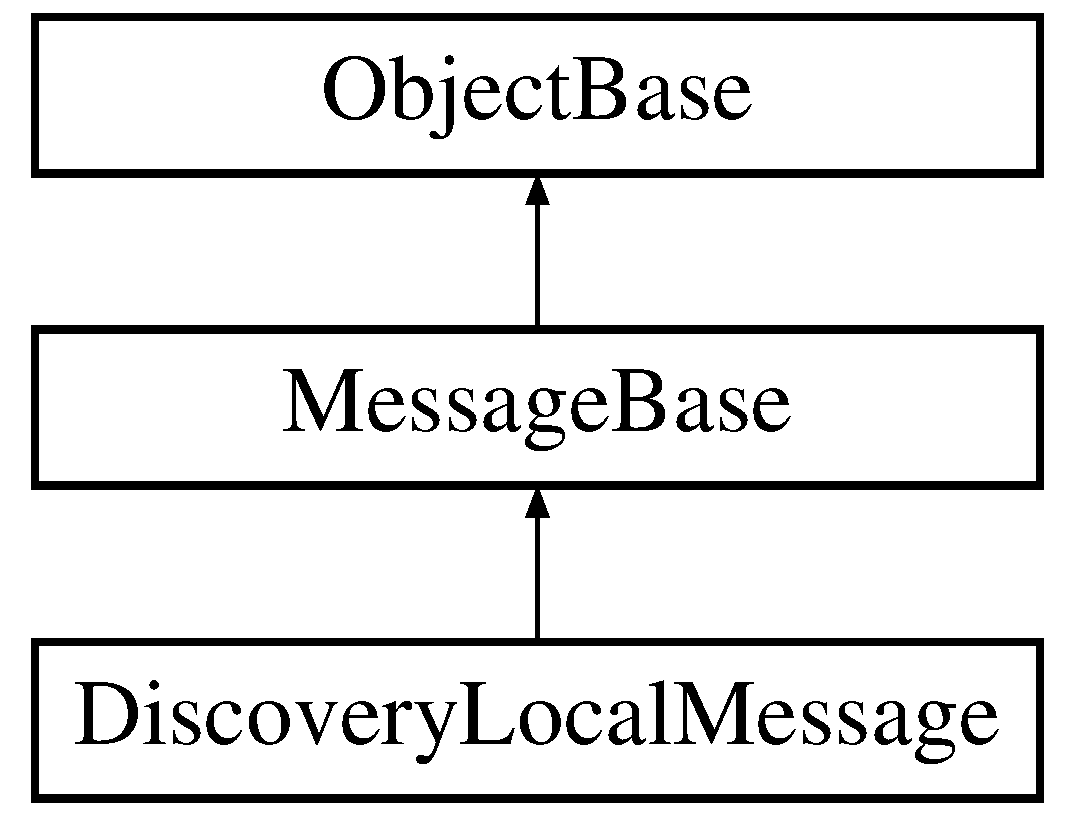
\includegraphics[height=3.000000cm]{classDiscoveryLocalMessage}
\end{center}
\end{figure}
\subsection*{Public Member Functions}
\begin{DoxyCompactItemize}
\item 
{\bf Discovery\+Local\+Message} (const {\bf Mailbox\+Address} \&source\+Address, Discovery\+Local\+Operation\+Type operation, const {\bf Mailbox\+Address} \&discovery\+Address)
\item 
{\bf Discovery\+Local\+Message} (const {\bf Discovery\+Local\+Message} \&rhs)
\item 
virtual {\bf $\sim$\+Discovery\+Local\+Message} ()
\item 
unsigned short {\bf get\+Message\+Id} () const 
\item 
Discovery\+Local\+Operation\+Type {\bf get\+Operation\+Type} () const 
\item 
const {\bf Mailbox\+Address} \& {\bf get\+Discovery\+Address} () const 
\item 
string {\bf to\+String} ()
\end{DoxyCompactItemize}
\subsection*{Additional Inherited Members}


\subsection{Constructor \& Destructor Documentation}
\index{Discovery\+Local\+Message@{Discovery\+Local\+Message}!Discovery\+Local\+Message@{Discovery\+Local\+Message}}
\index{Discovery\+Local\+Message@{Discovery\+Local\+Message}!Discovery\+Local\+Message@{Discovery\+Local\+Message}}
\subsubsection[{Discovery\+Local\+Message(const Mailbox\+Address \&source\+Address, Discovery\+Local\+Operation\+Type operation, const Mailbox\+Address \&discovery\+Address)}]{\setlength{\rightskip}{0pt plus 5cm}Discovery\+Local\+Message\+::\+Discovery\+Local\+Message (
\begin{DoxyParamCaption}
\item[{const {\bf Mailbox\+Address} \&}]{source\+Address, }
\item[{Discovery\+Local\+Operation\+Type}]{operation, }
\item[{const {\bf Mailbox\+Address} \&}]{discovery\+Address}
\end{DoxyParamCaption}
)}\label{classDiscoveryLocalMessage_a16707e9c2ee936fab2b7ad6b62e630fa}
Constructor 
\begin{DoxyParams}{Parameters}
{\em source\+Address} & Mailbox Address for this \doxyref{Discovery\+Manager}{p.}{classDiscoveryManager} (on this node) \\
\hline
{\em operation} & Type of discovery operation (register, deregister, display, etc.) \\
\hline
{\em discovery\+Address} & Mailbox Address that is being registered/deregistered \\
\hline
\end{DoxyParams}
\index{Discovery\+Local\+Message@{Discovery\+Local\+Message}!Discovery\+Local\+Message@{Discovery\+Local\+Message}}
\index{Discovery\+Local\+Message@{Discovery\+Local\+Message}!Discovery\+Local\+Message@{Discovery\+Local\+Message}}
\subsubsection[{Discovery\+Local\+Message(const Discovery\+Local\+Message \&rhs)}]{\setlength{\rightskip}{0pt plus 5cm}Discovery\+Local\+Message\+::\+Discovery\+Local\+Message (
\begin{DoxyParamCaption}
\item[{const {\bf Discovery\+Local\+Message} \&}]{rhs}
\end{DoxyParamCaption}
)}\label{classDiscoveryLocalMessage_af455006c5ec6fb9cf805d4c28bdcb23e}
Copy Constructor \index{Discovery\+Local\+Message@{Discovery\+Local\+Message}!````~Discovery\+Local\+Message@{$\sim$\+Discovery\+Local\+Message}}
\index{````~Discovery\+Local\+Message@{$\sim$\+Discovery\+Local\+Message}!Discovery\+Local\+Message@{Discovery\+Local\+Message}}
\subsubsection[{$\sim$\+Discovery\+Local\+Message()}]{\setlength{\rightskip}{0pt plus 5cm}Discovery\+Local\+Message\+::$\sim$\+Discovery\+Local\+Message (
\begin{DoxyParamCaption}
{}
\end{DoxyParamCaption}
)\hspace{0.3cm}{\ttfamily [virtual]}}\label{classDiscoveryLocalMessage_a9ee736c8d3adacb58afdca2e8beac3b4}
Virtual Destructor 

\subsection{Member Function Documentation}
\index{Discovery\+Local\+Message@{Discovery\+Local\+Message}!get\+Discovery\+Address@{get\+Discovery\+Address}}
\index{get\+Discovery\+Address@{get\+Discovery\+Address}!Discovery\+Local\+Message@{Discovery\+Local\+Message}}
\subsubsection[{get\+Discovery\+Address() const }]{\setlength{\rightskip}{0pt plus 5cm}const {\bf Mailbox\+Address} \& Discovery\+Local\+Message\+::get\+Discovery\+Address (
\begin{DoxyParamCaption}
{}
\end{DoxyParamCaption}
) const}\label{classDiscoveryLocalMessage_ae9e7e0165df5b5bd223d92101925b50d}
Returns the Discovery Address which is being registered/deregistered 

Referenced by Discovery\+Manager\+::process\+Mailbox().

\index{Discovery\+Local\+Message@{Discovery\+Local\+Message}!get\+Message\+Id@{get\+Message\+Id}}
\index{get\+Message\+Id@{get\+Message\+Id}!Discovery\+Local\+Message@{Discovery\+Local\+Message}}
\subsubsection[{get\+Message\+Id() const }]{\setlength{\rightskip}{0pt plus 5cm}unsigned short Discovery\+Local\+Message\+::get\+Message\+Id (
\begin{DoxyParamCaption}
{}
\end{DoxyParamCaption}
) const\hspace{0.3cm}{\ttfamily [virtual]}}\label{classDiscoveryLocalMessage_ab92d12523115997153625ededd0bba75}
Returns the Message Id 

Implements {\bf Message\+Base} \doxyref{}{p.}{classMessageBase_a0910c23e94ea98b7a4e11631c9068311}.

\index{Discovery\+Local\+Message@{Discovery\+Local\+Message}!get\+Operation\+Type@{get\+Operation\+Type}}
\index{get\+Operation\+Type@{get\+Operation\+Type}!Discovery\+Local\+Message@{Discovery\+Local\+Message}}
\subsubsection[{get\+Operation\+Type() const }]{\setlength{\rightskip}{0pt plus 5cm}Discovery\+Local\+Operation\+Type Discovery\+Local\+Message\+::get\+Operation\+Type (
\begin{DoxyParamCaption}
{}
\end{DoxyParamCaption}
) const}\label{classDiscoveryLocalMessage_aee363ebc41915eef8f67ee809c0a1c75}
Returns the Discovery Operation type 

Referenced by Discovery\+Manager\+::process\+Mailbox().

\index{Discovery\+Local\+Message@{Discovery\+Local\+Message}!to\+String@{to\+String}}
\index{to\+String@{to\+String}!Discovery\+Local\+Message@{Discovery\+Local\+Message}}
\subsubsection[{to\+String()}]{\setlength{\rightskip}{0pt plus 5cm}string Discovery\+Local\+Message\+::to\+String (
\begin{DoxyParamCaption}
{}
\end{DoxyParamCaption}
)\hspace{0.3cm}{\ttfamily [virtual]}}\label{classDiscoveryLocalMessage_ab31c4b11d9381989006819ab0463f27b}
String\textquotesingle{}ized debugging method \begin{DoxyReturn}{Returns}
string representation of the contents of this object 
\end{DoxyReturn}


Implements {\bf Message\+Base} \doxyref{}{p.}{classMessageBase_a7946fdcef86bfd67ad1df2ede8ed671d}.



References Message\+Base\+::source\+Address\+\_\+, and Mailbox\+Address\+::to\+String().



Referenced by Discovery\+Manager\+::process\+Mailbox().



The documentation for this class was generated from the following files\+:\begin{DoxyCompactItemize}
\item 
Discovery\+Local\+Message.\+h\item 
Discovery\+Local\+Message.\+cpp\end{DoxyCompactItemize}

\section{Discovery\+Manager Class Reference}
\label{classDiscoveryManager}\index{Discovery\+Manager@{Discovery\+Manager}}
\subsection*{Public Member Functions}
\begin{DoxyCompactItemize}
\item 
{\bf Discovery\+Manager} ()
\item 
virtual {\bf $\sim$\+Discovery\+Manager} ()
\item 
int {\bf initialize} ()
\item 
int {\bf register\+For\+Discovery\+Updates} (vector$<$ {\bf Mailbox\+Address} $>$ \&currently\+Registered\+Addresses, {\bf Mailbox\+Address} \&match\+Criteria, {\bf Mailbox\+Owner\+Handle} $\ast$mailbox\+To\+Notify)
\item 
int {\bf deregister\+For\+Discovery\+Updates} ({\bf Mailbox\+Owner\+Handle} $\ast$mailbox\+To\+Notify)
\item 
int {\bf register\+Local\+Address} ({\bf Mailbox\+Address} \&local\+Remote\+Type\+Address)
\item 
int {\bf deregister\+Local\+Address} ({\bf Mailbox\+Address} \&local\+Remote\+Type\+Address)
\item 
void {\bf list\+All\+Mailbox\+Addresses} ()
\item 
void {\bf process\+Mailbox} ()
\end{DoxyCompactItemize}


\subsection{Constructor \& Destructor Documentation}
\index{Discovery\+Manager@{Discovery\+Manager}!Discovery\+Manager@{Discovery\+Manager}}
\index{Discovery\+Manager@{Discovery\+Manager}!Discovery\+Manager@{Discovery\+Manager}}
\subsubsection[{Discovery\+Manager()}]{\setlength{\rightskip}{0pt plus 5cm}Discovery\+Manager\+::\+Discovery\+Manager (
\begin{DoxyParamCaption}
{}
\end{DoxyParamCaption}
)}\label{classDiscoveryManager_aed0e13d6e72ab0b0595c47682a33f1a0}
Constructor 

References System\+Info\+::get\+Local\+N\+E\+I\+D(), Mailbox\+Address\+::inet\+Address, Mailbox\+Address\+::location\+Type, Mailbox\+Address\+::mailbox\+Name, and Mailbox\+Address\+::neid.

\index{Discovery\+Manager@{Discovery\+Manager}!````~Discovery\+Manager@{$\sim$\+Discovery\+Manager}}
\index{````~Discovery\+Manager@{$\sim$\+Discovery\+Manager}!Discovery\+Manager@{Discovery\+Manager}}
\subsubsection[{$\sim$\+Discovery\+Manager()}]{\setlength{\rightskip}{0pt plus 5cm}Discovery\+Manager\+::$\sim$\+Discovery\+Manager (
\begin{DoxyParamCaption}
{}
\end{DoxyParamCaption}
)\hspace{0.3cm}{\ttfamily [virtual]}}\label{classDiscoveryManager_a46b24a0aceacc21190a39c6052c5143e}
Virtual Destructor 

\subsection{Member Function Documentation}
\index{Discovery\+Manager@{Discovery\+Manager}!deregister\+For\+Discovery\+Updates@{deregister\+For\+Discovery\+Updates}}
\index{deregister\+For\+Discovery\+Updates@{deregister\+For\+Discovery\+Updates}!Discovery\+Manager@{Discovery\+Manager}}
\subsubsection[{deregister\+For\+Discovery\+Updates(\+Mailbox\+Owner\+Handle $\ast$mailbox\+To\+Notify)}]{\setlength{\rightskip}{0pt plus 5cm}int Discovery\+Manager\+::deregister\+For\+Discovery\+Updates (
\begin{DoxyParamCaption}
\item[{{\bf Mailbox\+Owner\+Handle} $\ast$}]{mailbox\+To\+Notify}
\end{DoxyParamCaption}
)}\label{classDiscoveryManager_a72976ec911ad5f6d6dadbf6a08194ff2}
Allows mailboxes to deregister for Discovery Update notifications \begin{DoxyReturn}{Returns}
OK upon success; otherwise E\+R\+R\+OR 
\end{DoxyReturn}


Referenced by Mailbox\+Lookup\+Service\+::deregister\+Mailbox().

\index{Discovery\+Manager@{Discovery\+Manager}!deregister\+Local\+Address@{deregister\+Local\+Address}}
\index{deregister\+Local\+Address@{deregister\+Local\+Address}!Discovery\+Manager@{Discovery\+Manager}}
\subsubsection[{deregister\+Local\+Address(\+Mailbox\+Address \&local\+Remote\+Type\+Address)}]{\setlength{\rightskip}{0pt plus 5cm}int Discovery\+Manager\+::deregister\+Local\+Address (
\begin{DoxyParamCaption}
\item[{{\bf Mailbox\+Address} \&}]{local\+Remote\+Type\+Address}
\end{DoxyParamCaption}
)}\label{classDiscoveryManager_ac7ffe28660fc54012599c22d52208554}
Remove the local registration of a remote type Non-\/\+Proxy \doxyref{Mailbox\+Address}{p.}{structMailboxAddress}. This will facilitate a discovery D\+E\+R\+E\+G\+I\+S\+T\+ER update being sent to all other Discovery\+Managers. \begin{DoxyReturn}{Returns}
OK upon successful registration; otherwise E\+R\+R\+OR 
\end{DoxyReturn}


References Mailbox\+Owner\+Handle\+::post().



Referenced by Mailbox\+Lookup\+Service\+::deregister\+Mailbox().

\index{Discovery\+Manager@{Discovery\+Manager}!initialize@{initialize}}
\index{initialize@{initialize}!Discovery\+Manager@{Discovery\+Manager}}
\subsubsection[{initialize()}]{\setlength{\rightskip}{0pt plus 5cm}int Discovery\+Manager\+::initialize (
\begin{DoxyParamCaption}
{}
\end{DoxyParamCaption}
)}\label{classDiscoveryManager_ab4ede1f7bdf5e15ae869dfd34294f0ba}
Perform initialization of Discovery Manager which communicates mailbox updates between distributed nodes. \begin{DoxyReturn}{Returns}
OK upon success; otherwise E\+R\+R\+OR 
\end{DoxyReturn}


References Mailbox\+Owner\+Handle\+::activate(), Message\+Handler\+List\+::add(), Group\+Mailbox\+::create\+Mailbox(), Discovery\+Message\+::deserialize(), and Message\+Factory\+::register\+Support().



Referenced by Mailbox\+Lookup\+Service\+::initialize\+Discovery\+Manager().

\index{Discovery\+Manager@{Discovery\+Manager}!list\+All\+Mailbox\+Addresses@{list\+All\+Mailbox\+Addresses}}
\index{list\+All\+Mailbox\+Addresses@{list\+All\+Mailbox\+Addresses}!Discovery\+Manager@{Discovery\+Manager}}
\subsubsection[{list\+All\+Mailbox\+Addresses()}]{\setlength{\rightskip}{0pt plus 5cm}void Discovery\+Manager\+::list\+All\+Mailbox\+Addresses (
\begin{DoxyParamCaption}
{}
\end{DoxyParamCaption}
)}\label{classDiscoveryManager_a7dd229bdb52456987c057c70fbdaf158}
Display a list of all the registered remote type Non-\/\+Proxy mailbox addresses This method displays its output in trace logs. 

References Mailbox\+Owner\+Handle\+::post().



Referenced by Mailbox\+Lookup\+Service\+::list\+All\+Mailbox\+Addresses().

\index{Discovery\+Manager@{Discovery\+Manager}!process\+Mailbox@{process\+Mailbox}}
\index{process\+Mailbox@{process\+Mailbox}!Discovery\+Manager@{Discovery\+Manager}}
\subsubsection[{process\+Mailbox()}]{\setlength{\rightskip}{0pt plus 5cm}void Discovery\+Manager\+::process\+Mailbox (
\begin{DoxyParamCaption}
{}
\end{DoxyParamCaption}
)}\label{classDiscoveryManager_a283c87c3116b5ad99604af150a99cb65}
Start the mailbox processing loop 

References Mailbox\+Owner\+Handle\+::activate(), Group\+Mailbox\+Proxy\+::create\+Mailbox(), Discovery\+Message\+::get\+Discovery\+Address(), Discovery\+Local\+Message\+::get\+Discovery\+Address(), Discovery\+Message\+::get\+Operation\+Type(), Discovery\+Local\+Message\+::get\+Operation\+Type(), Discovery\+Message\+::get\+Originating\+P\+I\+D(), Message\+Base\+::get\+Source\+Address(), Mailbox\+Address\+::is\+Matching\+Address(), Mailbox\+Owner\+Handle\+::post(), Mailbox\+Processor\+::process\+Mailbox(), Mailbox\+Owner\+Handle\+::set\+Debug\+Value(), Discovery\+Local\+Message\+::to\+String(), Discovery\+Message\+::to\+String(), and Mailbox\+Address\+::to\+String().



Referenced by Mailbox\+Lookup\+Service\+::get\+Debug\+For\+All\+Mailbox\+Addresses().

\index{Discovery\+Manager@{Discovery\+Manager}!register\+For\+Discovery\+Updates@{register\+For\+Discovery\+Updates}}
\index{register\+For\+Discovery\+Updates@{register\+For\+Discovery\+Updates}!Discovery\+Manager@{Discovery\+Manager}}
\subsubsection[{register\+For\+Discovery\+Updates(vector$<$ Mailbox\+Address $>$ \&currently\+Registered\+Addresses, Mailbox\+Address \&match\+Criteria, Mailbox\+Owner\+Handle $\ast$mailbox\+To\+Notify)}]{\setlength{\rightskip}{0pt plus 5cm}int Discovery\+Manager\+::register\+For\+Discovery\+Updates (
\begin{DoxyParamCaption}
\item[{vector$<$ {\bf Mailbox\+Address} $>$ \&}]{currently\+Registered\+Addresses, }
\item[{{\bf Mailbox\+Address} \&}]{match\+Criteria, }
\item[{{\bf Mailbox\+Owner\+Handle} $\ast$}]{mailbox\+To\+Notify}
\end{DoxyParamCaption}
)}\label{classDiscoveryManager_ad298a98899cb55f659f9bd4fcfacb2b5}
Allows mailboxes to register for Discovery Update notifications. If a \doxyref{Discovery\+Message}{p.}{classDiscoveryMessage} update is received whose discovery Mailbox Address matches that of the match\+Criteria, then a copy of the \doxyref{Discovery\+Message}{p.}{classDiscoveryMessage} is posted to the mailbox\+To\+Notify. The caller is required to pre-\/allocate a vector of Mailbox\+Addresses which will be populated with \textquotesingle{}already-\/discovered\textquotesingle{} Mailbox\+Addresses and returned. 

Note that current there is no support for a user-\/initiated deregistration mechanism. This is because the discovery update mechanism should not be used as a substitute for I\+PC between nodes. 


\begin{DoxyParams}{Parameters}
{\em match\+Criteria} & \doxyref{Mailbox\+Address}{p.}{structMailboxAddress} object used to determine which discovery Mailbox Addresses match what the application wants to be notified about. N\+O\+TE\+: The calling application should leave all fields default except those that the caller wished to be used in the match comparison. For example, if the caller wants to be notified when any Mailboxes with the Mailbox\+Name \textquotesingle{}Call\+Processor\textquotesingle{} are discovered, the match\+Criteria field \textquotesingle{}Mailbox\+Name\textquotesingle{} will be set to \textquotesingle{}Call\+Processor\textquotesingle{} and all other fields left as the default. \\
\hline
{\em mailbox\+To\+Notify} & \doxyref{Mailbox\+Owner\+Handle}{p.}{classMailboxOwnerHandle} of the mailbox that will receive the \doxyref{Discovery\+Message}{p.}{classDiscoveryMessage} notification when an update is received. This mailbox must provide a Message\+Handler method for the Discovery Message id (M\+S\+G\+M\+G\+R\+\_\+\+D\+I\+S\+C\+O\+V\+E\+R\+Y\+\_\+\+M\+S\+G\+\_\+\+ID) \\
\hline
\end{DoxyParams}
\begin{DoxyReturn}{Returns}
OK upon successful registration; otherwise E\+R\+R\+OR 
\end{DoxyReturn}


References Mailbox\+Address\+::is\+Matching\+Address().



Referenced by Mailbox\+Lookup\+Service\+::register\+For\+Discovery\+Updates().

\index{Discovery\+Manager@{Discovery\+Manager}!register\+Local\+Address@{register\+Local\+Address}}
\index{register\+Local\+Address@{register\+Local\+Address}!Discovery\+Manager@{Discovery\+Manager}}
\subsubsection[{register\+Local\+Address(\+Mailbox\+Address \&local\+Remote\+Type\+Address)}]{\setlength{\rightskip}{0pt plus 5cm}int Discovery\+Manager\+::register\+Local\+Address (
\begin{DoxyParamCaption}
\item[{{\bf Mailbox\+Address} \&}]{local\+Remote\+Type\+Address}
\end{DoxyParamCaption}
)}\label{classDiscoveryManager_a2639330443e70d8c6acfa7794225b3f6}
Add local registration of a remote type Non-\/\+Proxy Mailbox Address. This will facilitate a discovery R\+E\+G\+I\+S\+T\+ER update being sent to all other Discovery\+Managers \begin{DoxyReturn}{Returns}
OK upon successful registration; otherwise E\+R\+R\+OR 
\end{DoxyReturn}


References Mailbox\+Owner\+Handle\+::post().



Referenced by Mailbox\+Lookup\+Service\+::register\+Mailbox().



The documentation for this class was generated from the following files\+:\begin{DoxyCompactItemize}
\item 
Discovery\+Manager.\+h\item 
Discovery\+Manager.\+cpp\end{DoxyCompactItemize}

\section{Discovery\+Message Class Reference}
\label{classDiscoveryMessage}\index{Discovery\+Message@{Discovery\+Message}}
Inheritance diagram for Discovery\+Message\+:\begin{figure}[H]
\begin{center}
\leavevmode
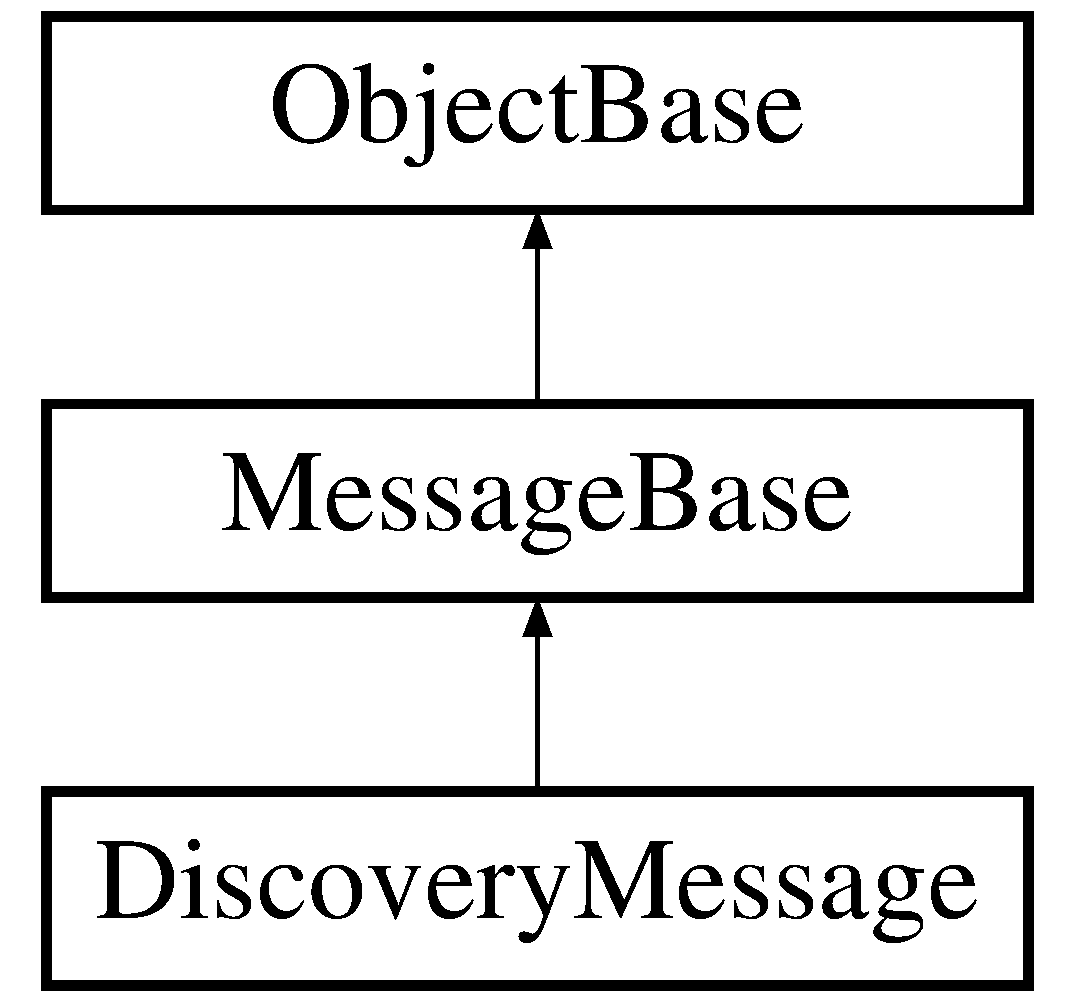
\includegraphics[height=3.000000cm]{classDiscoveryMessage}
\end{center}
\end{figure}
\subsection*{Public Member Functions}
\begin{DoxyCompactItemize}
\item 
{\bf Discovery\+Message} (const {\bf Mailbox\+Address} \&source\+Address, Discovery\+Operation\+Type operation, unsigned int originating\+P\+ID, const {\bf Mailbox\+Address} \&discovery\+Address)
\item 
{\bf Discovery\+Message} (const {\bf Discovery\+Message} \&rhs)
\item 
virtual {\bf $\sim$\+Discovery\+Message} ()
\item 
unsigned short {\bf get\+Message\+Id} () const 
\item 
Discovery\+Operation\+Type {\bf get\+Operation\+Type} () const 
\item 
const {\bf Mailbox\+Address} \& {\bf get\+Discovery\+Address} () const 
\item 
unsigned int {\bf get\+Originating\+P\+ID} () const 
\item 
int {\bf serialize} ({\bf Message\+Buffer} \&buffer)
\item 
string {\bf to\+String} ()
\end{DoxyCompactItemize}
\subsection*{Static Public Member Functions}
\begin{DoxyCompactItemize}
\item 
static {\bf Message\+Base} $\ast$ {\bf deserialize} ({\bf Message\+Buffer} $\ast$buffer)
\end{DoxyCompactItemize}
\subsection*{Additional Inherited Members}


\subsection{Constructor \& Destructor Documentation}
\index{Discovery\+Message@{Discovery\+Message}!Discovery\+Message@{Discovery\+Message}}
\index{Discovery\+Message@{Discovery\+Message}!Discovery\+Message@{Discovery\+Message}}
\subsubsection[{Discovery\+Message(const Mailbox\+Address \&source\+Address, Discovery\+Operation\+Type operation, unsigned int originating\+P\+I\+D, const Mailbox\+Address \&discovery\+Address)}]{\setlength{\rightskip}{0pt plus 5cm}Discovery\+Message\+::\+Discovery\+Message (
\begin{DoxyParamCaption}
\item[{const {\bf Mailbox\+Address} \&}]{source\+Address, }
\item[{Discovery\+Operation\+Type}]{operation, }
\item[{unsigned int}]{originating\+P\+ID, }
\item[{const {\bf Mailbox\+Address} \&}]{discovery\+Address}
\end{DoxyParamCaption}
)}\label{classDiscoveryMessage_ada416a276490cb49f8c3a31930f99dbe}
Constructor 
\begin{DoxyParams}{Parameters}
{\em source\+Address} & Mailbox Address for this \doxyref{Discovery\+Manager}{p.}{classDiscoveryManager} (on this node) \\
\hline
{\em operation} & Type of discovery operation (register, deregister, etc.) \\
\hline
{\em discovery\+Address} & Mailbox Address that is being registered/deregistered \\
\hline
\end{DoxyParams}


Referenced by deserialize().

\index{Discovery\+Message@{Discovery\+Message}!Discovery\+Message@{Discovery\+Message}}
\index{Discovery\+Message@{Discovery\+Message}!Discovery\+Message@{Discovery\+Message}}
\subsubsection[{Discovery\+Message(const Discovery\+Message \&rhs)}]{\setlength{\rightskip}{0pt plus 5cm}Discovery\+Message\+::\+Discovery\+Message (
\begin{DoxyParamCaption}
\item[{const {\bf Discovery\+Message} \&}]{rhs}
\end{DoxyParamCaption}
)}\label{classDiscoveryMessage_aa54db081cf8826e1824177be13c03c88}
Copy Constructor \index{Discovery\+Message@{Discovery\+Message}!````~Discovery\+Message@{$\sim$\+Discovery\+Message}}
\index{````~Discovery\+Message@{$\sim$\+Discovery\+Message}!Discovery\+Message@{Discovery\+Message}}
\subsubsection[{$\sim$\+Discovery\+Message()}]{\setlength{\rightskip}{0pt plus 5cm}Discovery\+Message\+::$\sim$\+Discovery\+Message (
\begin{DoxyParamCaption}
{}
\end{DoxyParamCaption}
)\hspace{0.3cm}{\ttfamily [virtual]}}\label{classDiscoveryMessage_a9b1210d21a4135761ff9c964892ffdeb}
Virtual Destructor 

\subsection{Member Function Documentation}
\index{Discovery\+Message@{Discovery\+Message}!deserialize@{deserialize}}
\index{deserialize@{deserialize}!Discovery\+Message@{Discovery\+Message}}
\subsubsection[{deserialize(\+Message\+Buffer $\ast$buffer)}]{\setlength{\rightskip}{0pt plus 5cm}{\bf Message\+Base} $\ast$ Discovery\+Message\+::deserialize (
\begin{DoxyParamCaption}
\item[{{\bf Message\+Buffer} $\ast$}]{buffer}
\end{DoxyParamCaption}
)\hspace{0.3cm}{\ttfamily [static]}}\label{classDiscoveryMessage_ae76860a9afec759af6545aabd75a7adb}
Subclassed deserialization / bootstrap implementation 

References Discovery\+Message().



Referenced by Discovery\+Manager\+::initialize().

\index{Discovery\+Message@{Discovery\+Message}!get\+Discovery\+Address@{get\+Discovery\+Address}}
\index{get\+Discovery\+Address@{get\+Discovery\+Address}!Discovery\+Message@{Discovery\+Message}}
\subsubsection[{get\+Discovery\+Address() const }]{\setlength{\rightskip}{0pt plus 5cm}const {\bf Mailbox\+Address} \& Discovery\+Message\+::get\+Discovery\+Address (
\begin{DoxyParamCaption}
{}
\end{DoxyParamCaption}
) const}\label{classDiscoveryMessage_a7a78388064fe97844b531014bf016409}
Returns the Discovery Address which is being registered/deregistered 

Referenced by Discovery\+Manager\+::process\+Mailbox().

\index{Discovery\+Message@{Discovery\+Message}!get\+Message\+Id@{get\+Message\+Id}}
\index{get\+Message\+Id@{get\+Message\+Id}!Discovery\+Message@{Discovery\+Message}}
\subsubsection[{get\+Message\+Id() const }]{\setlength{\rightskip}{0pt plus 5cm}unsigned short Discovery\+Message\+::get\+Message\+Id (
\begin{DoxyParamCaption}
{}
\end{DoxyParamCaption}
) const\hspace{0.3cm}{\ttfamily [virtual]}}\label{classDiscoveryMessage_ad208d214bd5b00595bd3869425d9bdc7}
Returns the Message Id 

Implements {\bf Message\+Base} \doxyref{}{p.}{classMessageBase_a0910c23e94ea98b7a4e11631c9068311}.

\index{Discovery\+Message@{Discovery\+Message}!get\+Operation\+Type@{get\+Operation\+Type}}
\index{get\+Operation\+Type@{get\+Operation\+Type}!Discovery\+Message@{Discovery\+Message}}
\subsubsection[{get\+Operation\+Type() const }]{\setlength{\rightskip}{0pt plus 5cm}Discovery\+Operation\+Type Discovery\+Message\+::get\+Operation\+Type (
\begin{DoxyParamCaption}
{}
\end{DoxyParamCaption}
) const}\label{classDiscoveryMessage_a7027d866945417ea159a59a32aa6b0bd}
Returns the Discovery Operation type 

Referenced by Discovery\+Manager\+::process\+Mailbox().

\index{Discovery\+Message@{Discovery\+Message}!get\+Originating\+P\+ID@{get\+Originating\+P\+ID}}
\index{get\+Originating\+P\+ID@{get\+Originating\+P\+ID}!Discovery\+Message@{Discovery\+Message}}
\subsubsection[{get\+Originating\+P\+I\+D() const }]{\setlength{\rightskip}{0pt plus 5cm}unsigned int Discovery\+Message\+::get\+Originating\+P\+ID (
\begin{DoxyParamCaption}
{}
\end{DoxyParamCaption}
) const}\label{classDiscoveryMessage_a2bcbf6451d657d7ae514ba642f331772}
Returns the P\+ID of the process that originated this message. Used to verify and filter out messages from our own \doxyref{Discovery\+Manager}{p.}{classDiscoveryManager} 

Referenced by Discovery\+Manager\+::process\+Mailbox().

\index{Discovery\+Message@{Discovery\+Message}!serialize@{serialize}}
\index{serialize@{serialize}!Discovery\+Message@{Discovery\+Message}}
\subsubsection[{serialize(\+Message\+Buffer \&buffer)}]{\setlength{\rightskip}{0pt plus 5cm}int Discovery\+Message\+::serialize (
\begin{DoxyParamCaption}
\item[{{\bf Message\+Buffer} \&}]{buffer}
\end{DoxyParamCaption}
)\hspace{0.3cm}{\ttfamily [virtual]}}\label{classDiscoveryMessage_af7192abcad9f42eec25e303435740382}
Subclassed serialization implementation 

Reimplemented from {\bf Message\+Base} \doxyref{}{p.}{classMessageBase_a1120deb2887e4a72d7dc68b505e5e10a}.



References Message\+Base\+::source\+Address\+\_\+.

\index{Discovery\+Message@{Discovery\+Message}!to\+String@{to\+String}}
\index{to\+String@{to\+String}!Discovery\+Message@{Discovery\+Message}}
\subsubsection[{to\+String()}]{\setlength{\rightskip}{0pt plus 5cm}string Discovery\+Message\+::to\+String (
\begin{DoxyParamCaption}
{}
\end{DoxyParamCaption}
)\hspace{0.3cm}{\ttfamily [virtual]}}\label{classDiscoveryMessage_aee9ec66013b69b35b672679e91d4118c}
String\textquotesingle{}ized debugging method \begin{DoxyReturn}{Returns}
string representation of the contents of this object 
\end{DoxyReturn}


Implements {\bf Message\+Base} \doxyref{}{p.}{classMessageBase_a7946fdcef86bfd67ad1df2ede8ed671d}.



References Message\+Base\+::source\+Address\+\_\+, and Mailbox\+Address\+::to\+String().



Referenced by Discovery\+Manager\+::process\+Mailbox().



The documentation for this class was generated from the following files\+:\begin{DoxyCompactItemize}
\item 
Discovery\+Message.\+h\item 
Discovery\+Message.\+cpp\end{DoxyCompactItemize}

\section{Distributed\+Mailbox Class Reference}
\label{classDistributedMailbox}\index{Distributed\+Mailbox@{Distributed\+Mailbox}}
Inheritance diagram for Distributed\+Mailbox\+:\begin{figure}[H]
\begin{center}
\leavevmode
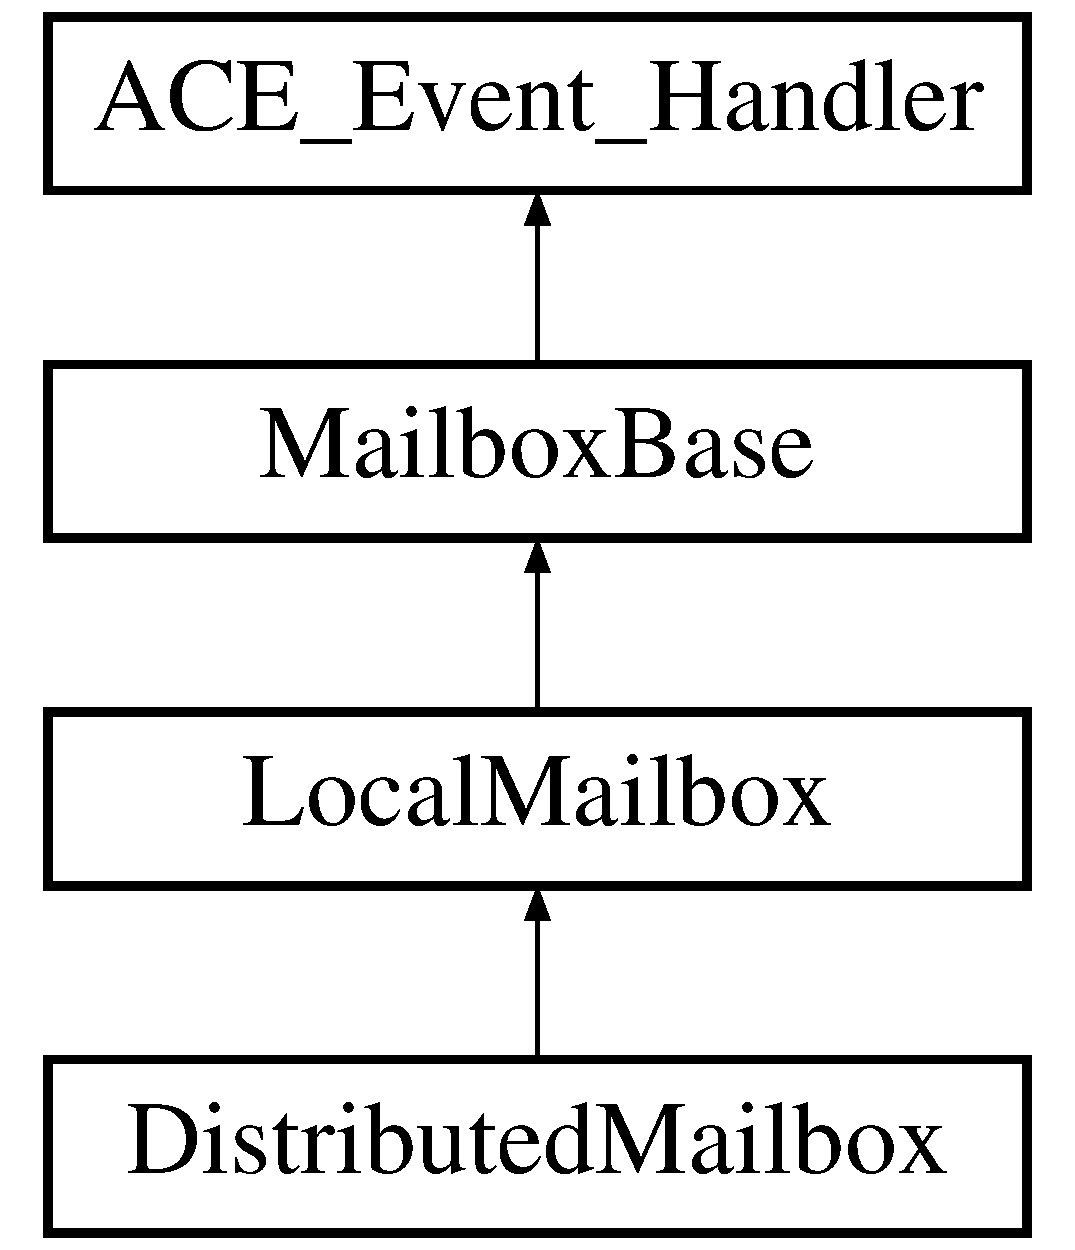
\includegraphics[height=4.000000cm]{classDistributedMailbox}
\end{center}
\end{figure}
\subsection*{Public Types}
\begin{DoxyCompactItemize}
\item 
typedef map$<$ A\+C\+E\+\_\+\+H\+A\+N\+D\+LE, A\+C\+E\+\_\+\+S\+O\+C\+K\+\_\+\+Stream $\ast$ $>$ {\bf Client\+Connector\+Map}
\end{DoxyCompactItemize}
\subsection*{Public Member Functions}
\begin{DoxyCompactItemize}
\item 
virtual bool {\bf rename} (const {\bf Mailbox\+Address} \&new\+Remote\+Address)
\item 
virtual int {\bf activate} ({\bf Mailbox\+Owner\+Handle} $\ast$mailbox\+Owner\+Handle)
\item 
virtual int {\bf deactivate} ({\bf Mailbox\+Owner\+Handle} $\ast$mailbox\+Owner\+Handle)
\item 
{\bf Mailbox\+Address} \& {\bf get\+Mailbox\+Address} ()
\item 
string {\bf to\+String} ()
\end{DoxyCompactItemize}
\subsection*{Static Public Member Functions}
\begin{DoxyCompactItemize}
\item 
static {\bf Mailbox\+Owner\+Handle} $\ast$ {\bf create\+Mailbox} (const {\bf Mailbox\+Address} \&remote\+Address)
\end{DoxyCompactItemize}
\subsection*{Protected Member Functions}
\begin{DoxyCompactItemize}
\item 
{\bf Distributed\+Mailbox} (const {\bf Mailbox\+Address} \&distributed\+Address)
\item 
virtual {\bf $\sim$\+Distributed\+Mailbox} ()
\end{DoxyCompactItemize}
\subsection*{Additional Inherited Members}


\subsection{Member Typedef Documentation}
\index{Distributed\+Mailbox@{Distributed\+Mailbox}!Client\+Connector\+Map@{Client\+Connector\+Map}}
\index{Client\+Connector\+Map@{Client\+Connector\+Map}!Distributed\+Mailbox@{Distributed\+Mailbox}}
\subsubsection[{Client\+Connector\+Map}]{\setlength{\rightskip}{0pt plus 5cm}typedef map$<$A\+C\+E\+\_\+\+H\+A\+N\+D\+LE, A\+C\+E\+\_\+\+S\+O\+C\+K\+\_\+\+Stream$\ast$$>$ {\bf Distributed\+Mailbox\+::\+Client\+Connector\+Map}}\label{classDistributedMailbox_ac1120c8bf3cd549e79ec451a4c578b47}
Create a map for storing A\+C\+E\+\_\+\+H\+A\+N\+D\+L\+Es and their associated A\+C\+E\+\_\+\+S\+O\+C\+K\+\_\+\+Stream objects. Each map entry corresponds to a single client \textquotesingle{}connector\textquotesingle{} connection to this distributed mailbox. 

\subsection{Constructor \& Destructor Documentation}
\index{Distributed\+Mailbox@{Distributed\+Mailbox}!Distributed\+Mailbox@{Distributed\+Mailbox}}
\index{Distributed\+Mailbox@{Distributed\+Mailbox}!Distributed\+Mailbox@{Distributed\+Mailbox}}
\subsubsection[{Distributed\+Mailbox(const Mailbox\+Address \&distributed\+Address)}]{\setlength{\rightskip}{0pt plus 5cm}Distributed\+Mailbox\+::\+Distributed\+Mailbox (
\begin{DoxyParamCaption}
\item[{const {\bf Mailbox\+Address} \&}]{distributed\+Address}
\end{DoxyParamCaption}
)\hspace{0.3cm}{\ttfamily [protected]}}\label{classDistributedMailbox_a82d60016a270ca2b9c70bc1c9e673860}
Constructor -\/ protected so that applications cannot create their own mailboxes and must use the static \doxyref{create\+Mailbox()}{p.}{classDistributedMailbox_a58ee18029660253156c84afb579266ca} method 

References Distributed\+Mailbox().



Referenced by Distributed\+Mailbox().

\index{Distributed\+Mailbox@{Distributed\+Mailbox}!````~Distributed\+Mailbox@{$\sim$\+Distributed\+Mailbox}}
\index{````~Distributed\+Mailbox@{$\sim$\+Distributed\+Mailbox}!Distributed\+Mailbox@{Distributed\+Mailbox}}
\subsubsection[{$\sim$\+Distributed\+Mailbox()}]{\setlength{\rightskip}{0pt plus 5cm}Distributed\+Mailbox\+::$\sim$\+Distributed\+Mailbox (
\begin{DoxyParamCaption}
{}
\end{DoxyParamCaption}
)\hspace{0.3cm}{\ttfamily [protected]}, {\ttfamily [virtual]}}\label{classDistributedMailbox_a36078b97601728b58736ee6ee3af450f}
Virtual Destructor. Protected since this is a reference counted object. 

References Mailbox\+Base\+::is\+Shutting\+Down\+\_\+.



\subsection{Member Function Documentation}
\index{Distributed\+Mailbox@{Distributed\+Mailbox}!activate@{activate}}
\index{activate@{activate}!Distributed\+Mailbox@{Distributed\+Mailbox}}
\subsubsection[{activate(\+Mailbox\+Owner\+Handle $\ast$mailbox\+Owner\+Handle)}]{\setlength{\rightskip}{0pt plus 5cm}int Distributed\+Mailbox\+::activate (
\begin{DoxyParamCaption}
\item[{{\bf Mailbox\+Owner\+Handle} $\ast$}]{mailbox\+Owner\+Handle}
\end{DoxyParamCaption}
)\hspace{0.3cm}{\ttfamily [virtual]}}\label{classDistributedMailbox_ace1358b217d0f0a52be4d32e3277c211}
Activate the mailbox. For security, one must possess an Owner Handle in order to activate the mailbox and register it with the Lookup Service. 

Reimplemented from {\bf Local\+Mailbox} \doxyref{}{p.}{classLocalMailbox_a90a0b182b76f38934302d613c74b626f}.



References Local\+Mailbox\+::activate(), Local\+Mailbox\+::deactivate(), Mailbox\+Address\+::inet\+Address, and Mailbox\+Base\+::is\+Active().

\index{Distributed\+Mailbox@{Distributed\+Mailbox}!create\+Mailbox@{create\+Mailbox}}
\index{create\+Mailbox@{create\+Mailbox}!Distributed\+Mailbox@{Distributed\+Mailbox}}
\subsubsection[{create\+Mailbox(const Mailbox\+Address \&remote\+Address)}]{\setlength{\rightskip}{0pt plus 5cm}{\bf Mailbox\+Owner\+Handle} $\ast$ Distributed\+Mailbox\+::create\+Mailbox (
\begin{DoxyParamCaption}
\item[{const {\bf Mailbox\+Address} \&}]{remote\+Address}
\end{DoxyParamCaption}
)\hspace{0.3cm}{\ttfamily [static]}}\label{classDistributedMailbox_a58ee18029660253156c84afb579266ca}
Allows applications to create a mailbox and get a handle to it.

Since we do not want applications to have direct access to a mailbox object this method is provided. Applications that create mailboxes use this method to get a handle to their mailbox rather than have direct access. The handle returned is a owner handle which has all the privileges of the actual mailbox (get\+Message/post etc). This method creates the mailbox, activates it (which in turn registers it with the lookup service) and then creates an owner handle, acquires it and then returns that handle. Both the mailbox and the returned handle are created on the heap. 

References Message\+Buffer\+::are\+Contents\+Processed(), Message\+Buffer\+::clear\+Buffer(), Thread\+Manager\+::create\+Thread(), Mailbox\+Base\+::debug\+Value\+\_\+, Message\+Buffer\+::get\+Buffer(), Message\+Base\+::get\+Message\+Id(), Message\+Base\+::get\+Source\+Address(), Mailbox\+Base\+::increment\+Received\+Count(), Mailbox\+Address\+::inet\+Address, Mailbox\+Address\+::location\+Type, Local\+Mailbox\+::post(), Message\+Factory\+::recreate\+Message\+From\+Buffer(), Mailbox\+Base\+::select\+Reactor\+\_\+, Message\+Buffer\+::set\+Insert\+Position(), Message\+Base\+::set\+Priority(), Local\+Mailbox\+::start\+Reactor(), and Message\+Base\+::to\+String().



Referenced by Fault\+Manager\+::process\+Mailbox(), and Resource\+Monitor\+::to\+String().

\index{Distributed\+Mailbox@{Distributed\+Mailbox}!deactivate@{deactivate}}
\index{deactivate@{deactivate}!Distributed\+Mailbox@{Distributed\+Mailbox}}
\subsubsection[{deactivate(\+Mailbox\+Owner\+Handle $\ast$mailbox\+Owner\+Handle)}]{\setlength{\rightskip}{0pt plus 5cm}int Distributed\+Mailbox\+::deactivate (
\begin{DoxyParamCaption}
\item[{{\bf Mailbox\+Owner\+Handle} $\ast$}]{mailbox\+Owner\+Handle}
\end{DoxyParamCaption}
)\hspace{0.3cm}{\ttfamily [virtual]}}\label{classDistributedMailbox_ab02bba7663485f4747afe81030737981}
Deactivate the mailbox. For security, one must possess an Owner Handle in order to deactivate the mailbox and deregister it with the Lookup Service. 

Reimplemented from {\bf Local\+Mailbox} \doxyref{}{p.}{classLocalMailbox_a257122f75a72d9cbba8692cd1d8c431c}.



References Local\+Mailbox\+::deactivate().

\index{Distributed\+Mailbox@{Distributed\+Mailbox}!get\+Mailbox\+Address@{get\+Mailbox\+Address}}
\index{get\+Mailbox\+Address@{get\+Mailbox\+Address}!Distributed\+Mailbox@{Distributed\+Mailbox}}
\subsubsection[{get\+Mailbox\+Address()}]{\setlength{\rightskip}{0pt plus 5cm}{\bf Mailbox\+Address} \& Distributed\+Mailbox\+::get\+Mailbox\+Address (
\begin{DoxyParamCaption}
{}
\end{DoxyParamCaption}
)\hspace{0.3cm}{\ttfamily [virtual]}}\label{classDistributedMailbox_a2e729a806eaae2187e41b7286e2bb6a9}
Return the mailbox distributed address 

Implements {\bf Mailbox\+Base} \doxyref{}{p.}{classMailboxBase_ace28a599cdadf1afa99c94602eb7e4a6}.



References Mailbox\+Base\+::is\+Shutting\+Down\+\_\+.

\index{Distributed\+Mailbox@{Distributed\+Mailbox}!rename@{rename}}
\index{rename@{rename}!Distributed\+Mailbox@{Distributed\+Mailbox}}
\subsubsection[{rename(const Mailbox\+Address \&new\+Remote\+Address)}]{\setlength{\rightskip}{0pt plus 5cm}bool Distributed\+Mailbox\+::rename (
\begin{DoxyParamCaption}
\item[{const {\bf Mailbox\+Address} \&}]{new\+Remote\+Address}
\end{DoxyParamCaption}
)\hspace{0.3cm}{\ttfamily [virtual]}}\label{classDistributedMailbox_afdfc26662bae3b128ab4832e2c9fbbac}
Method to allow application to rename a mailbox\textquotesingle{}s remote address.

T\+BD\+: What are the redundancy implications and usage here?? 

Reimplemented from {\bf Mailbox\+Base} \doxyref{}{p.}{classMailboxBase_a93bf1108b770d273af5c4282bdcdfe47}.

\index{Distributed\+Mailbox@{Distributed\+Mailbox}!to\+String@{to\+String}}
\index{to\+String@{to\+String}!Distributed\+Mailbox@{Distributed\+Mailbox}}
\subsubsection[{to\+String()}]{\setlength{\rightskip}{0pt plus 5cm}string Distributed\+Mailbox\+::to\+String (
\begin{DoxyParamCaption}
{}
\end{DoxyParamCaption}
)}\label{classDistributedMailbox_a352dc799d41c42a5e8768fb89c027cb8}
String\textquotesingle{}ized debugging method \begin{DoxyReturn}{Returns}
string representation of the contents of this object 
\end{DoxyReturn}


The documentation for this class was generated from the following files\+:\begin{DoxyCompactItemize}
\item 
Distributed\+Mailbox.\+h\item 
Distributed\+Mailbox.\+cpp\end{DoxyCompactItemize}

\section{Distributed\+Mailbox\+Proxy Class Reference}
\label{classDistributedMailboxProxy}\index{Distributed\+Mailbox\+Proxy@{Distributed\+Mailbox\+Proxy}}
Inheritance diagram for Distributed\+Mailbox\+Proxy\+:\begin{figure}[H]
\begin{center}
\leavevmode
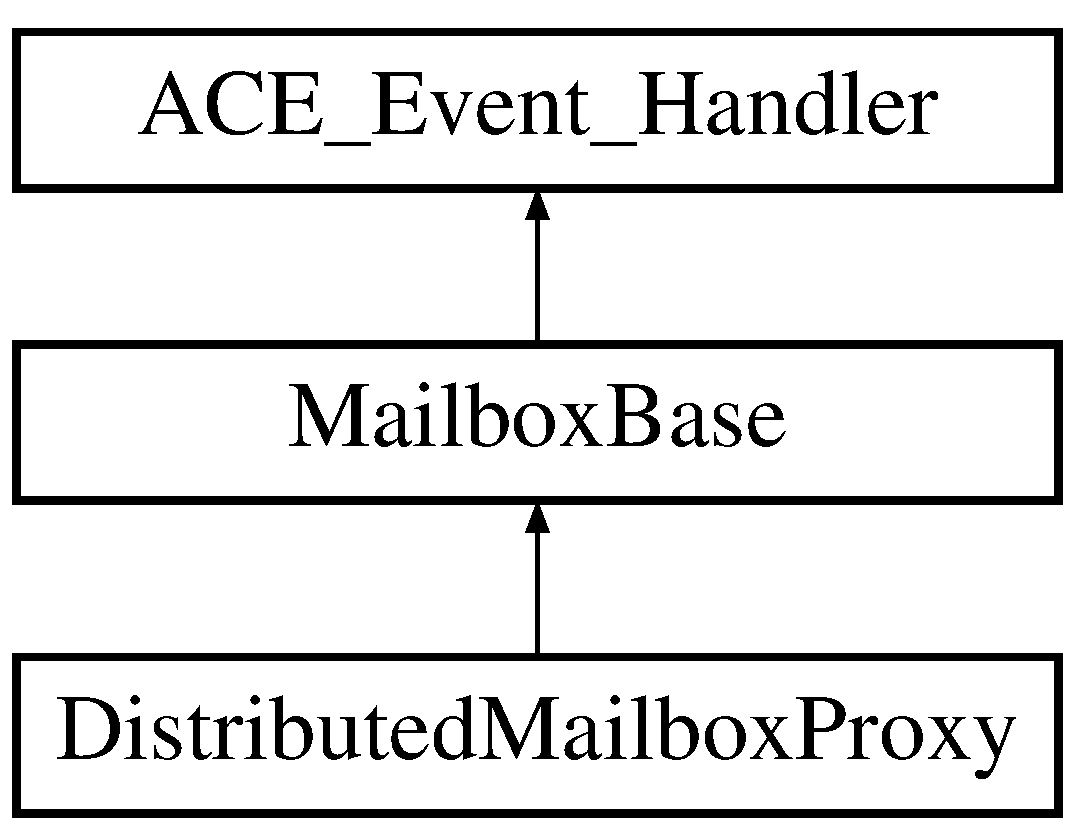
\includegraphics[height=3.000000cm]{classDistributedMailboxProxy}
\end{center}
\end{figure}
\subsection*{Public Member Functions}
\begin{DoxyCompactItemize}
\item 
virtual int {\bf post} ({\bf Message\+Base} $\ast$message\+Ptr, const A\+C\+E\+\_\+\+Time\+\_\+\+Value $\ast$timeout=\&A\+C\+E\+\_\+\+Time\+\_\+\+Value\+::zero)
\item 
virtual int {\bf activate} ({\bf Mailbox\+Owner\+Handle} $\ast$mailbox\+Owner\+Handle)
\item 
virtual int {\bf deactivate} ({\bf Mailbox\+Owner\+Handle} $\ast$mailbox\+Owner\+Handle)
\item 
virtual const A\+C\+E\+\_\+\+Time\+\_\+\+Value \& {\bf get\+Post\+Default\+Timeout} ()
\item 
virtual int {\bf get\+Debug\+Value} ()
\item 
virtual void {\bf set\+Debug\+Value} (int debug\+Value)
\item 
{\bf Mailbox\+Address} \& {\bf get\+Mailbox\+Address} ()
\item 
string {\bf to\+String} ()
\end{DoxyCompactItemize}
\subsection*{Static Public Member Functions}
\begin{DoxyCompactItemize}
\item 
static {\bf Mailbox\+Owner\+Handle} $\ast$ {\bf create\+Mailbox} (const {\bf Mailbox\+Address} \&remote\+Address)
\end{DoxyCompactItemize}
\subsection*{Protected Member Functions}
\begin{DoxyCompactItemize}
\item 
{\bf Distributed\+Mailbox\+Proxy} (const {\bf Mailbox\+Address} \&remote\+Address)
\item 
virtual {\bf $\sim$\+Distributed\+Mailbox\+Proxy} ()
\end{DoxyCompactItemize}
\subsection*{Additional Inherited Members}


\subsection{Constructor \& Destructor Documentation}
\index{Distributed\+Mailbox\+Proxy@{Distributed\+Mailbox\+Proxy}!Distributed\+Mailbox\+Proxy@{Distributed\+Mailbox\+Proxy}}
\index{Distributed\+Mailbox\+Proxy@{Distributed\+Mailbox\+Proxy}!Distributed\+Mailbox\+Proxy@{Distributed\+Mailbox\+Proxy}}
\subsubsection[{Distributed\+Mailbox\+Proxy(const Mailbox\+Address \&remote\+Address)}]{\setlength{\rightskip}{0pt plus 5cm}Distributed\+Mailbox\+Proxy\+::\+Distributed\+Mailbox\+Proxy (
\begin{DoxyParamCaption}
\item[{const {\bf Mailbox\+Address} \&}]{remote\+Address}
\end{DoxyParamCaption}
)\hspace{0.3cm}{\ttfamily [protected]}}\label{classDistributedMailboxProxy_a529676c5c5d33eae4814bb08b847b3e9}
Constructor 

References O\+P\+M\+::create\+Pool(), Distributed\+Mailbox\+Proxy(), Message\+Buffer\+::initialize(), and Mailbox\+Base\+::is\+Proxy\+\_\+.



Referenced by Distributed\+Mailbox\+Proxy().

\index{Distributed\+Mailbox\+Proxy@{Distributed\+Mailbox\+Proxy}!````~Distributed\+Mailbox\+Proxy@{$\sim$\+Distributed\+Mailbox\+Proxy}}
\index{````~Distributed\+Mailbox\+Proxy@{$\sim$\+Distributed\+Mailbox\+Proxy}!Distributed\+Mailbox\+Proxy@{Distributed\+Mailbox\+Proxy}}
\subsubsection[{$\sim$\+Distributed\+Mailbox\+Proxy()}]{\setlength{\rightskip}{0pt plus 5cm}Distributed\+Mailbox\+Proxy\+::$\sim$\+Distributed\+Mailbox\+Proxy (
\begin{DoxyParamCaption}
{}
\end{DoxyParamCaption}
)\hspace{0.3cm}{\ttfamily [protected]}, {\ttfamily [virtual]}}\label{classDistributedMailboxProxy_a7bc239e37eb849e0dc8037dbebb621e6}
Virtual Destructor. Protected since this is a reference counted object. 

References Mailbox\+Base\+::is\+Shutting\+Down\+\_\+.



\subsection{Member Function Documentation}
\index{Distributed\+Mailbox\+Proxy@{Distributed\+Mailbox\+Proxy}!activate@{activate}}
\index{activate@{activate}!Distributed\+Mailbox\+Proxy@{Distributed\+Mailbox\+Proxy}}
\subsubsection[{activate(\+Mailbox\+Owner\+Handle $\ast$mailbox\+Owner\+Handle)}]{\setlength{\rightskip}{0pt plus 5cm}int Distributed\+Mailbox\+Proxy\+::activate (
\begin{DoxyParamCaption}
\item[{{\bf Mailbox\+Owner\+Handle} $\ast$}]{mailbox\+Owner\+Handle}
\end{DoxyParamCaption}
)\hspace{0.3cm}{\ttfamily [virtual]}}\label{classDistributedMailboxProxy_a0eca78d4f87db3a4237fc972e6f187e9}
Activate the mailbox. For security, one must possess an Owner Handle to activate the mailbox and register it with the Lookup Service. 

Reimplemented from {\bf Mailbox\+Base} \doxyref{}{p.}{classMailboxBase_a98c6c4736af9c084d5395d7a4303ec67}.



References Mailbox\+Address\+::inet\+Address, Mailbox\+Base\+::is\+Active(), Mailbox\+Lookup\+Service\+::register\+Mailbox(), and Mailbox\+Base\+::set\+Active().

\index{Distributed\+Mailbox\+Proxy@{Distributed\+Mailbox\+Proxy}!create\+Mailbox@{create\+Mailbox}}
\index{create\+Mailbox@{create\+Mailbox}!Distributed\+Mailbox\+Proxy@{Distributed\+Mailbox\+Proxy}}
\subsubsection[{create\+Mailbox(const Mailbox\+Address \&remote\+Address)}]{\setlength{\rightskip}{0pt plus 5cm}{\bf Mailbox\+Owner\+Handle} $\ast$ Distributed\+Mailbox\+Proxy\+::create\+Mailbox (
\begin{DoxyParamCaption}
\item[{const {\bf Mailbox\+Address} \&}]{remote\+Address}
\end{DoxyParamCaption}
)\hspace{0.3cm}{\ttfamily [static]}}\label{classDistributedMailboxProxy_a4b680a5ef52a6eaab732df6dd0c8eebb}
Allows applications to create a mailbox and get a handle to it.

Since we do not want applications to have direct access to a mailbox object this method is provided. Applications that create mailboxes use this method to get a handle to their mailbox rather than have direct access. The handle returned is a owner handle which has all the privileges of the actual mailbox (get\+Message/post etc). This method creates the mailbox, activates it (which in turn registers it with the lookup service) and then creates an owner handle, acquires it and then returns that handle. Both the mailbox and the returned handle are created on the heap. 

Referenced by Mailbox\+Lookup\+Service\+::find().

\index{Distributed\+Mailbox\+Proxy@{Distributed\+Mailbox\+Proxy}!deactivate@{deactivate}}
\index{deactivate@{deactivate}!Distributed\+Mailbox\+Proxy@{Distributed\+Mailbox\+Proxy}}
\subsubsection[{deactivate(\+Mailbox\+Owner\+Handle $\ast$mailbox\+Owner\+Handle)}]{\setlength{\rightskip}{0pt plus 5cm}int Distributed\+Mailbox\+Proxy\+::deactivate (
\begin{DoxyParamCaption}
\item[{{\bf Mailbox\+Owner\+Handle} $\ast$}]{mailbox\+Owner\+Handle}
\end{DoxyParamCaption}
)\hspace{0.3cm}{\ttfamily [virtual]}}\label{classDistributedMailboxProxy_a4d984ccc9f6591abd671e9eb6dadbcc4}
Deactivate the mailbox. For security, one must possess an Owner Handle to deactivate the mailbox and deregister it with the Lookup Service. 

Reimplemented from {\bf Mailbox\+Base} \doxyref{}{p.}{classMailboxBase_a14ba6bd7936f32ecb51763acb89c507c}.



References Mailbox\+Lookup\+Service\+::deregister\+Mailbox(), Mailbox\+Base\+::is\+Active(), and Mailbox\+Base\+::set\+Active().

\index{Distributed\+Mailbox\+Proxy@{Distributed\+Mailbox\+Proxy}!get\+Debug\+Value@{get\+Debug\+Value}}
\index{get\+Debug\+Value@{get\+Debug\+Value}!Distributed\+Mailbox\+Proxy@{Distributed\+Mailbox\+Proxy}}
\subsubsection[{get\+Debug\+Value()}]{\setlength{\rightskip}{0pt plus 5cm}int Distributed\+Mailbox\+Proxy\+::get\+Debug\+Value (
\begin{DoxyParamCaption}
{}
\end{DoxyParamCaption}
)\hspace{0.3cm}{\ttfamily [virtual]}}\label{classDistributedMailboxProxy_a36039bde300d10e2b5dc104e1e61a057}
Return the debug flag 

Implements {\bf Mailbox\+Base} \doxyref{}{p.}{classMailboxBase_af5d9b331f7cb55d27517def24cc16de6}.



References Mailbox\+Base\+::debug\+Value\+\_\+.

\index{Distributed\+Mailbox\+Proxy@{Distributed\+Mailbox\+Proxy}!get\+Mailbox\+Address@{get\+Mailbox\+Address}}
\index{get\+Mailbox\+Address@{get\+Mailbox\+Address}!Distributed\+Mailbox\+Proxy@{Distributed\+Mailbox\+Proxy}}
\subsubsection[{get\+Mailbox\+Address()}]{\setlength{\rightskip}{0pt plus 5cm}{\bf Mailbox\+Address} \& Distributed\+Mailbox\+Proxy\+::get\+Mailbox\+Address (
\begin{DoxyParamCaption}
{}
\end{DoxyParamCaption}
)\hspace{0.3cm}{\ttfamily [virtual]}}\label{classDistributedMailboxProxy_ab1263cbe93c584d84022b480190e7080}
Return the mailbox distributed address 

Implements {\bf Mailbox\+Base} \doxyref{}{p.}{classMailboxBase_ace28a599cdadf1afa99c94602eb7e4a6}.

\index{Distributed\+Mailbox\+Proxy@{Distributed\+Mailbox\+Proxy}!get\+Post\+Default\+Timeout@{get\+Post\+Default\+Timeout}}
\index{get\+Post\+Default\+Timeout@{get\+Post\+Default\+Timeout}!Distributed\+Mailbox\+Proxy@{Distributed\+Mailbox\+Proxy}}
\subsubsection[{get\+Post\+Default\+Timeout()}]{\setlength{\rightskip}{0pt plus 5cm}const A\+C\+E\+\_\+\+Time\+\_\+\+Value \& Distributed\+Mailbox\+Proxy\+::get\+Post\+Default\+Timeout (
\begin{DoxyParamCaption}
{}
\end{DoxyParamCaption}
)\hspace{0.3cm}{\ttfamily [virtual]}}\label{classDistributedMailboxProxy_a413c9f5b24771d55bbacdab4f9bb20f5}
Return the appropriate default timeout for the \doxyref{post()}{p.}{classDistributedMailboxProxy_af73348ca55313a5e1a6b699ec9900cf7} 

Implements {\bf Mailbox\+Base} \doxyref{}{p.}{classMailboxBase_a7e288209b5f7daf305f8a882a6b806c6}.

\index{Distributed\+Mailbox\+Proxy@{Distributed\+Mailbox\+Proxy}!post@{post}}
\index{post@{post}!Distributed\+Mailbox\+Proxy@{Distributed\+Mailbox\+Proxy}}
\subsubsection[{post(\+Message\+Base $\ast$message\+Ptr, const A\+C\+E\+\_\+\+Time\+\_\+\+Value $\ast$timeout=\&\+A\+C\+E\+\_\+\+Time\+\_\+\+Value\+::zero)}]{\setlength{\rightskip}{0pt plus 5cm}int Distributed\+Mailbox\+Proxy\+::post (
\begin{DoxyParamCaption}
\item[{{\bf Message\+Base} $\ast$}]{message\+Ptr, }
\item[{const A\+C\+E\+\_\+\+Time\+\_\+\+Value $\ast$}]{timeout = {\ttfamily \&ACE\+\_\+Time\+\_\+Value\+:\+:zero}}
\end{DoxyParamCaption}
)\hspace{0.3cm}{\ttfamily [virtual]}}\label{classDistributedMailboxProxy_af73348ca55313a5e1a6b699ec9900cf7}
Post a message to the distributed remote mailbox. Subclass implementations should examine the \char`\"{}active\+\_\+\char`\"{} state. Upon initial failure of the post, this proxy mailbox will close and re-\/open the socket and attempt to post the message again automatically. If the the repost fails, then E\+R\+R\+OR will be returned, and it becomes the responsibility of the application to retry the message after deleting the mailbox handle and performing \doxyref{Mailbox\+Lookup\+Service\+::find}{p.}{classMailboxLookupService_a04a96883cc551682e635924884e433ac} (which may return a redundant mate\textquotesingle{}s handle); or, the application can give up and delete the message off of the heap. \begin{DoxyReturn}{Returns}
zero for an error, non-\/zero otherwise. 
\end{DoxyReturn}


Implements {\bf Mailbox\+Base} \doxyref{}{p.}{classMailboxBase_a6ac15f4fcc8493e7cc1e79310f1129a7}.



References Mailbox\+Base\+::debug\+Value\+\_\+, Message\+Base\+::delete\+Message(), Message\+Base\+::get\+Message\+Id(), Message\+Base\+::get\+Priority(), Message\+Base\+::get\+Source\+Address(), Mailbox\+Base\+::increment\+Sent\+Count(), Mailbox\+Address\+::inet\+Address, Mailbox\+Base\+::is\+Active(), Message\+Base\+::serialize(), Message\+Base\+::to\+String(), and Mailbox\+Address\+::to\+String().

\index{Distributed\+Mailbox\+Proxy@{Distributed\+Mailbox\+Proxy}!set\+Debug\+Value@{set\+Debug\+Value}}
\index{set\+Debug\+Value@{set\+Debug\+Value}!Distributed\+Mailbox\+Proxy@{Distributed\+Mailbox\+Proxy}}
\subsubsection[{set\+Debug\+Value(int debug\+Value)}]{\setlength{\rightskip}{0pt plus 5cm}void Distributed\+Mailbox\+Proxy\+::set\+Debug\+Value (
\begin{DoxyParamCaption}
\item[{int}]{debug\+Value}
\end{DoxyParamCaption}
)\hspace{0.3cm}{\ttfamily [virtual]}}\label{classDistributedMailboxProxy_a993b782f3aeb9a15c17271169b0442a0}
Set the debug flag 

Implements {\bf Mailbox\+Base} \doxyref{}{p.}{classMailboxBase_a3be54965c1fafbc4de3d7e6087128a4f}.



References Mailbox\+Base\+::debug\+Value\+\_\+.

\index{Distributed\+Mailbox\+Proxy@{Distributed\+Mailbox\+Proxy}!to\+String@{to\+String}}
\index{to\+String@{to\+String}!Distributed\+Mailbox\+Proxy@{Distributed\+Mailbox\+Proxy}}
\subsubsection[{to\+String()}]{\setlength{\rightskip}{0pt plus 5cm}string Distributed\+Mailbox\+Proxy\+::to\+String (
\begin{DoxyParamCaption}
{}
\end{DoxyParamCaption}
)}\label{classDistributedMailboxProxy_a5838564ce52194552e6f26eaf270d391}
String\textquotesingle{}ized debugging method \begin{DoxyReturn}{Returns}
string representation of the contents of this object 
\end{DoxyReturn}


The documentation for this class was generated from the following files\+:\begin{DoxyCompactItemize}
\item 
Distributed\+Mailbox\+Proxy.\+h\item 
Distributed\+Mailbox\+Proxy.\+cpp\end{DoxyCompactItemize}

\section{C\+B\+Functor\+Base\+:\+:Dummy\+Init Class Reference}
\label{classCBFunctorBase_1_1DummyInit}\index{C\+B\+Functor\+Base\+::\+Dummy\+Init@{C\+B\+Functor\+Base\+::\+Dummy\+Init}}


The documentation for this class was generated from the following file\+:\begin{DoxyCompactItemize}
\item 
Callback.\+h\end{DoxyCompactItemize}

\section{Fault\+Manager Class Reference}
\label{classFaultManager}\index{Fault\+Manager@{Fault\+Manager}}
\subsection*{Public Member Functions}
\begin{DoxyCompactItemize}
\item 
{\bf Fault\+Manager} ()
\item 
virtual {\bf $\sim$\+Fault\+Manager} ()
\item 
void {\bf process\+Mailbox} ()
\item 
int {\bf initialize} (int fault\+Report\+Period)
\end{DoxyCompactItemize}
\subsection*{Static Public Member Functions}
\begin{DoxyCompactItemize}
\item 
static void {\bf catch\+Shutdown\+Signal} ()
\end{DoxyCompactItemize}


\subsection{Constructor \& Destructor Documentation}
\index{Fault\+Manager@{Fault\+Manager}!Fault\+Manager@{Fault\+Manager}}
\index{Fault\+Manager@{Fault\+Manager}!Fault\+Manager@{Fault\+Manager}}
\subsubsection[{Fault\+Manager()}]{\setlength{\rightskip}{0pt plus 5cm}Fault\+Manager\+::\+Fault\+Manager (
\begin{DoxyParamCaption}
{}
\end{DoxyParamCaption}
)}\label{classFaultManager_a793298ebd1f43384765dd39e8ae27075}
Constructor 

Referenced by process\+Mailbox().

\index{Fault\+Manager@{Fault\+Manager}!````~Fault\+Manager@{$\sim$\+Fault\+Manager}}
\index{````~Fault\+Manager@{$\sim$\+Fault\+Manager}!Fault\+Manager@{Fault\+Manager}}
\subsubsection[{$\sim$\+Fault\+Manager()}]{\setlength{\rightskip}{0pt plus 5cm}Fault\+Manager\+::$\sim$\+Fault\+Manager (
\begin{DoxyParamCaption}
{}
\end{DoxyParamCaption}
)\hspace{0.3cm}{\ttfamily [virtual]}}\label{classFaultManager_a9fb6591326c4c19e22cf22759b0b73a5}
Virtual Destructor 

\subsection{Member Function Documentation}
\index{Fault\+Manager@{Fault\+Manager}!catch\+Shutdown\+Signal@{catch\+Shutdown\+Signal}}
\index{catch\+Shutdown\+Signal@{catch\+Shutdown\+Signal}!Fault\+Manager@{Fault\+Manager}}
\subsubsection[{catch\+Shutdown\+Signal()}]{\setlength{\rightskip}{0pt plus 5cm}void Fault\+Manager\+::catch\+Shutdown\+Signal (
\begin{DoxyParamCaption}
{}
\end{DoxyParamCaption}
)\hspace{0.3cm}{\ttfamily [static]}}\label{classFaultManager_a2ab7c6bb0069ab06c3ec15c379c677d8}
Catch the shutdown signal and begin the graceful shutdown 

Referenced by initialize().

\index{Fault\+Manager@{Fault\+Manager}!initialize@{initialize}}
\index{initialize@{initialize}!Fault\+Manager@{Fault\+Manager}}
\subsubsection[{initialize(int fault\+Report\+Period)}]{\setlength{\rightskip}{0pt plus 5cm}int Fault\+Manager\+::initialize (
\begin{DoxyParamCaption}
\item[{int}]{fault\+Report\+Period}
\end{DoxyParamCaption}
)}\label{classFaultManager_a801cf6c046d9cebae73229a3378bcee1}
Perform \doxyref{Fault\+Manager}{p.}{classFaultManager} initialization 
\begin{DoxyParams}{Parameters}
{\em fault\+Report\+Period} & Interval period for which Fault Manager will publish a fault report of outstanding alarms in the trace logs \\
\hline
\end{DoxyParams}
\begin{DoxyReturn}{Returns}
E\+R\+R\+OR on failure; otherwise OK 
\end{DoxyReturn}


References Data\+Manager\+::activate\+Connection\+Set(), catch\+Shutdown\+Signal(), Thread\+Manager\+::create\+Thread(), Mailbox\+Lookup\+Service\+::find(), System\+Info\+::get\+Local\+N\+E\+I\+D(), Mailbox\+Address\+::inet\+Address, Data\+Manager\+::initialize(), Mailbox\+Address\+::location\+Type, Mailbox\+Address\+::mailbox\+Name, Mailbox\+Address\+::neid, Mailbox\+Owner\+Handle\+::schedule\+Timer(), and Fault\+S\+M\+Queue\+::setup\+Queue().



Referenced by process\+Mailbox().

\index{Fault\+Manager@{Fault\+Manager}!process\+Mailbox@{process\+Mailbox}}
\index{process\+Mailbox@{process\+Mailbox}!Fault\+Manager@{Fault\+Manager}}
\subsubsection[{process\+Mailbox()}]{\setlength{\rightskip}{0pt plus 5cm}void Fault\+Manager\+::process\+Mailbox (
\begin{DoxyParamCaption}
{}
\end{DoxyParamCaption}
)}\label{classFaultManager_a06321519c488763c07c6bf57be51556e}
Start the mailbox processing loop 

References Mailbox\+Owner\+Handle\+::activate(), Message\+Handler\+List\+::add(), Fault\+Message\+::alarm\+Code, Fault\+Message\+::alarm\+Severity, Db\+Connection\+Handle\+::close\+Command\+Result(), Distributed\+Mailbox\+::create\+Mailbox(), Fault\+S\+M\+Queue\+::dequeue\+Alarm(), Fault\+Message\+::event\+Code, Db\+Connection\+Handle\+::execute\+Command(), Fault\+Manager(), Mailbox\+Lookup\+Service\+::find(), Db\+Connection\+Handle\+::get\+Column\+Count(), Db\+Connection\+Handle\+::get\+Column\+Index(), Db\+Connection\+Handle\+::get\+Column\+Name(), Logger\+::get\+Instance(), Db\+Connection\+Handle\+::get\+Int\+Value\+At(), Mailbox\+Owner\+Handle\+::get\+Mailbox\+Address(), Db\+Connection\+Handle\+::get\+Row\+Count(), Db\+Connection\+Handle\+::get\+Short\+Value\+At(), Db\+Connection\+Handle\+::get\+String\+Value\+At(), Db\+Connection\+Handle\+::get\+Timestamp\+Value\+At(), O\+P\+M\+::initialize(), initialize(), Logger\+::initialize(), Fault\+S\+M\+Queue\+::is\+Empty(), Fault\+Message\+::managed\+Object, Fault\+Message\+::managed\+Object\+Instance, Fault\+Message\+::neid\+PI, Fault\+Message\+::pid, Mailbox\+Handle\+::post(), Mailbox\+Processor\+::process\+Mailbox(), process\+Mailbox(), Data\+Manager\+::release\+Connection(), Data\+Manager\+::reserve\+Connection(), Mailbox\+Lookup\+Service\+::set\+Debug\+For\+All\+Mailbox\+Addresses(), Mailbox\+Owner\+Handle\+::set\+Debug\+Value(), Logger\+::set\+Subsystem\+Log\+Level(), and Fault\+Message\+::time\+Stamp.



Referenced by process\+Mailbox().



The documentation for this class was generated from the following files\+:\begin{DoxyCompactItemize}
\item 
Fault\+Manager.\+h\item 
Fault\+Manager.\+cpp\end{DoxyCompactItemize}

\section{Fault\+Message Struct Reference}
\label{structFaultMessage}\index{Fault\+Message@{Fault\+Message}}
\subsection*{Public Member Functions}
\begin{DoxyCompactItemize}
\item 
{\bf Fault\+Message} ()
\item 
{\bf Fault\+Message} (const {\bf Fault\+Message} \&rhs)
\item 
{\bf $\sim$\+Fault\+Message} (void)
\item 
void {\bf reset} (void)
\item 
{\bf Fault\+Message} \& {\bf operator=} (const {\bf Fault\+Message} \&rhs)
\item 
bool {\bf operator==} (const {\bf Fault\+Message} \&rhs) const 
\item 
bool {\bf operator$<$} (const {\bf Fault\+Message} \&rhs) const 
\end{DoxyCompactItemize}
\subsection*{Public Attributes}
\begin{DoxyCompactItemize}
\item 
char {\bf neid} [N\+E\+I\+D\+\_\+\+L\+E\+N\+G\+TH]
\item 
A\+C\+E\+\_\+\+Based\+\_\+\+Pointer\+\_\+\+Basic$<$ char $>$ {\bf neid\+PI}
\item 
Managed\+Object\+Type {\bf managed\+Object}
\item 
unsigned int {\bf managed\+Object\+Instance}
\item 
Alarm\+Code\+Type {\bf alarm\+Code}
\item 
Event\+Code\+Type {\bf event\+Code}
\item 
Alarm\+Severity\+Type {\bf alarm\+Severity}
\item 
unsigned int {\bf pid}
\item 
unsigned int {\bf time\+Stamp}
\end{DoxyCompactItemize}


\subsection{Constructor \& Destructor Documentation}
\index{Fault\+Message@{Fault\+Message}!Fault\+Message@{Fault\+Message}}
\index{Fault\+Message@{Fault\+Message}!Fault\+Message@{Fault\+Message}}
\subsubsection[{Fault\+Message()}]{\setlength{\rightskip}{0pt plus 5cm}Fault\+Message\+::\+Fault\+Message (
\begin{DoxyParamCaption}
{}
\end{DoxyParamCaption}
)}\label{structFaultMessage_aee21d16af0af20e259631033e4073fee}
Default Constructor 

References neid, and neid\+PI.

\index{Fault\+Message@{Fault\+Message}!Fault\+Message@{Fault\+Message}}
\index{Fault\+Message@{Fault\+Message}!Fault\+Message@{Fault\+Message}}
\subsubsection[{Fault\+Message(const Fault\+Message \&rhs)}]{\setlength{\rightskip}{0pt plus 5cm}Fault\+Message\+::\+Fault\+Message (
\begin{DoxyParamCaption}
\item[{const {\bf Fault\+Message} \&}]{rhs}
\end{DoxyParamCaption}
)}\label{structFaultMessage_aad1811f08e881a2a4c60554eda811f89}
Copy Constructor 

References alarm\+Code, alarm\+Severity, event\+Code, managed\+Object, managed\+Object\+Instance, neid, neid\+PI, pid, and time\+Stamp.

\index{Fault\+Message@{Fault\+Message}!````~Fault\+Message@{$\sim$\+Fault\+Message}}
\index{````~Fault\+Message@{$\sim$\+Fault\+Message}!Fault\+Message@{Fault\+Message}}
\subsubsection[{$\sim$\+Fault\+Message(void)}]{\setlength{\rightskip}{0pt plus 5cm}Fault\+Message\+::$\sim$\+Fault\+Message (
\begin{DoxyParamCaption}
\item[{void}]{}
\end{DoxyParamCaption}
)}\label{structFaultMessage_a1c090e1fd6c1657e11a0aa2beb8e504e}
Destructor 

\subsection{Member Function Documentation}
\index{Fault\+Message@{Fault\+Message}!operator$<$@{operator$<$}}
\index{operator$<$@{operator$<$}!Fault\+Message@{Fault\+Message}}
\subsubsection[{operator$<$(const Fault\+Message \&rhs) const }]{\setlength{\rightskip}{0pt plus 5cm}bool Fault\+Message\+::operator$<$ (
\begin{DoxyParamCaption}
\item[{const {\bf Fault\+Message} \&}]{rhs}
\end{DoxyParamCaption}
) const}\label{structFaultMessage_af7c4d27d6f7729cea21439d8fa9b266b}
Overloaded comparison operator 

References alarm\+Code, alarm\+Severity, event\+Code, managed\+Object, managed\+Object\+Instance, neid\+PI, pid, and time\+Stamp.

\index{Fault\+Message@{Fault\+Message}!operator=@{operator=}}
\index{operator=@{operator=}!Fault\+Message@{Fault\+Message}}
\subsubsection[{operator=(const Fault\+Message \&rhs)}]{\setlength{\rightskip}{0pt plus 5cm}{\bf Fault\+Message} \& Fault\+Message\+::operator= (
\begin{DoxyParamCaption}
\item[{const {\bf Fault\+Message} \&}]{rhs}
\end{DoxyParamCaption}
)}\label{structFaultMessage_aa3a1b8a8bfb6cc8bfaa7145bdc71f3da}
Overloaded assignment operator 

References alarm\+Code, alarm\+Severity, event\+Code, managed\+Object, managed\+Object\+Instance, neid, neid\+PI, pid, and time\+Stamp.

\index{Fault\+Message@{Fault\+Message}!operator==@{operator==}}
\index{operator==@{operator==}!Fault\+Message@{Fault\+Message}}
\subsubsection[{operator==(const Fault\+Message \&rhs) const }]{\setlength{\rightskip}{0pt plus 5cm}bool Fault\+Message\+::operator== (
\begin{DoxyParamCaption}
\item[{const {\bf Fault\+Message} \&}]{rhs}
\end{DoxyParamCaption}
) const}\label{structFaultMessage_afd8f0d09202f017cd55339795c2ed65d}
Overloaded equality operator 

References alarm\+Code, alarm\+Severity, event\+Code, managed\+Object, managed\+Object\+Instance, neid\+PI, pid, and time\+Stamp.

\index{Fault\+Message@{Fault\+Message}!reset@{reset}}
\index{reset@{reset}!Fault\+Message@{Fault\+Message}}
\subsubsection[{reset(void)}]{\setlength{\rightskip}{0pt plus 5cm}void Fault\+Message\+::reset (
\begin{DoxyParamCaption}
\item[{void}]{}
\end{DoxyParamCaption}
)}\label{structFaultMessage_a7f190a980a73819bf7a63e6f26646e3c}
Reset data members 

References alarm\+Code, alarm\+Severity, event\+Code, managed\+Object, managed\+Object\+Instance, neid, neid\+PI, pid, and time\+Stamp.



\subsection{Member Data Documentation}
\index{Fault\+Message@{Fault\+Message}!alarm\+Code@{alarm\+Code}}
\index{alarm\+Code@{alarm\+Code}!Fault\+Message@{Fault\+Message}}
\subsubsection[{alarm\+Code}]{\setlength{\rightskip}{0pt plus 5cm}Alarm\+Code\+Type Fault\+Message\+::alarm\+Code}\label{structFaultMessage_a1cc9b6c3b4bf8b644fe9a814a0d25df2}
Alarm code that applies to the fault condition 

Referenced by Faults\+::clear\+Alarm(), Fault\+Message(), operator$<$(), operator=(), operator==(), Fault\+Manager\+::process\+Mailbox(), Faults\+::raise\+Alarm(), and reset().

\index{Fault\+Message@{Fault\+Message}!alarm\+Severity@{alarm\+Severity}}
\index{alarm\+Severity@{alarm\+Severity}!Fault\+Message@{Fault\+Message}}
\subsubsection[{alarm\+Severity}]{\setlength{\rightskip}{0pt plus 5cm}Alarm\+Severity\+Type Fault\+Message\+::alarm\+Severity}\label{structFaultMessage_a8f2f9744d6f2a76c82126ec72256a75d}
Severity. This field is used for event reports and clear alarms, but for raising alarms, this severity will be re-\/assigned/overriden by the severity in the database since we need to support severity reassignment by the user 

Referenced by Faults\+::clear\+Alarm(), Fault\+Message(), operator$<$(), operator=(), operator==(), Fault\+Manager\+::process\+Mailbox(), Faults\+::raise\+Alarm(), Faults\+::report\+Event(), and reset().

\index{Fault\+Message@{Fault\+Message}!event\+Code@{event\+Code}}
\index{event\+Code@{event\+Code}!Fault\+Message@{Fault\+Message}}
\subsubsection[{event\+Code}]{\setlength{\rightskip}{0pt plus 5cm}Event\+Code\+Type Fault\+Message\+::event\+Code}\label{structFaultMessage_a6e0ec292fcea91f8c40443f2c5123ead}
Event Report code if the fault message is an event report instead 

Referenced by Fault\+Message(), operator$<$(), operator=(), operator==(), Fault\+Manager\+::process\+Mailbox(), Faults\+::report\+Event(), and reset().

\index{Fault\+Message@{Fault\+Message}!managed\+Object@{managed\+Object}}
\index{managed\+Object@{managed\+Object}!Fault\+Message@{Fault\+Message}}
\subsubsection[{managed\+Object}]{\setlength{\rightskip}{0pt plus 5cm}Managed\+Object\+Type Fault\+Message\+::managed\+Object}\label{structFaultMessage_a338dc5f9d9d52a9478b474b584f82b9b}
Managed Object type (M\+E\+M\+O\+RY, C\+O\+M\+M\+U\+N\+I\+C\+A\+T\+I\+O\+NS L\+I\+NK, H\+A\+RD D\+I\+SK, etc.) 

Referenced by Faults\+::clear\+Alarm(), Fault\+Message(), operator$<$(), operator=(), operator==(), Fault\+Manager\+::process\+Mailbox(), Faults\+::raise\+Alarm(), Faults\+::report\+Event(), and reset().

\index{Fault\+Message@{Fault\+Message}!managed\+Object\+Instance@{managed\+Object\+Instance}}
\index{managed\+Object\+Instance@{managed\+Object\+Instance}!Fault\+Message@{Fault\+Message}}
\subsubsection[{managed\+Object\+Instance}]{\setlength{\rightskip}{0pt plus 5cm}unsigned int Fault\+Message\+::managed\+Object\+Instance}\label{structFaultMessage_af32676d42b21fe98ddd5bb3ebcf06b29}
Managed Object instance (L\+I\+NK 12, L\+I\+NK 13, etc.) 

Referenced by Faults\+::clear\+Alarm(), Fault\+Message(), operator$<$(), operator=(), operator==(), Fault\+Manager\+::process\+Mailbox(), Faults\+::raise\+Alarm(), Faults\+::report\+Event(), and reset().

\index{Fault\+Message@{Fault\+Message}!neid@{neid}}
\index{neid@{neid}!Fault\+Message@{Fault\+Message}}
\subsubsection[{neid}]{\setlength{\rightskip}{0pt plus 5cm}char Fault\+Message\+::neid[N\+E\+I\+D\+\_\+\+L\+E\+N\+G\+TH]}\label{structFaultMessage_ab9f4d48f5451798fb95dcca348118535}
N\+E\+ID (network element Id) that the Fault applies to. 9 character string 

Referenced by Faults\+::clear\+Alarm(), Fault\+Message(), operator=(), Faults\+::raise\+Alarm(), and reset().

\index{Fault\+Message@{Fault\+Message}!neid\+PI@{neid\+PI}}
\index{neid\+PI@{neid\+PI}!Fault\+Message@{Fault\+Message}}
\subsubsection[{neid\+PI}]{\setlength{\rightskip}{0pt plus 5cm}A\+C\+E\+\_\+\+Based\+\_\+\+Pointer\+\_\+\+Basic$<$char$>$ Fault\+Message\+::neid\+PI}\label{structFaultMessage_af4985a4765181e55dfdc16464f6b9c0a}
Position Independent pointer to the N\+E\+ID 

Referenced by Faults\+::clear\+Alarm(), Fault\+Message(), operator$<$(), operator=(), operator==(), Fault\+Manager\+::process\+Mailbox(), Faults\+::raise\+Alarm(), and reset().

\index{Fault\+Message@{Fault\+Message}!pid@{pid}}
\index{pid@{pid}!Fault\+Message@{Fault\+Message}}
\subsubsection[{pid}]{\setlength{\rightskip}{0pt plus 5cm}unsigned int Fault\+Message\+::pid}\label{structFaultMessage_a28230466de03857454649d3e16f84594}
OS Process ID originating the alarm 

Referenced by Faults\+::clear\+Alarm(), Fault\+Message(), operator$<$(), operator=(), operator==(), Fault\+Manager\+::process\+Mailbox(), Faults\+::raise\+Alarm(), Faults\+::report\+Event(), and reset().

\index{Fault\+Message@{Fault\+Message}!time\+Stamp@{time\+Stamp}}
\index{time\+Stamp@{time\+Stamp}!Fault\+Message@{Fault\+Message}}
\subsubsection[{time\+Stamp}]{\setlength{\rightskip}{0pt plus 5cm}unsigned int Fault\+Message\+::time\+Stamp}\label{structFaultMessage_a22b2d875be78a7143b0916f5e86fd1f4}
Time stamp for alarm origination 

Referenced by Faults\+::clear\+Alarm(), Fault\+Message(), operator$<$(), operator=(), operator==(), Fault\+Manager\+::process\+Mailbox(), Faults\+::raise\+Alarm(), Faults\+::report\+Event(), and reset().



The documentation for this struct was generated from the following files\+:\begin{DoxyCompactItemize}
\item 
Fault\+Message.\+h\item 
Fault\+Message.\+cpp\end{DoxyCompactItemize}

\section{Faults Class Reference}
\label{classFaults}\index{Faults@{Faults}}


{\ttfamily \#include $<$Faults.\+h$>$}

\subsection*{Public Member Functions}
\begin{DoxyCompactItemize}
\item 
{\bf $\sim$\+Faults} ()
\item 
int {\bf initialize} ()
\end{DoxyCompactItemize}
\subsection*{Static Public Member Functions}
\begin{DoxyCompactItemize}
\item 
static void {\bf raise\+Alarm} (const char $\ast$neid, Alarm\+Code\+Type alarmcode, Managed\+Object\+Type managed\+Object, unsigned int managed\+Object\+Instance, unsigned int pid)
\item 
static void {\bf clear\+Alarm} (const char $\ast$neid, Alarm\+Code\+Type alarmcode, Managed\+Object\+Type managed\+Object, unsigned int managed\+Object\+Instance, unsigned int pid)
\item 
static void {\bf report\+Event} (Event\+Code\+Type eventcode, Managed\+Object\+Type managed\+Object, unsigned int managed\+Object\+Instance, unsigned int pid)
\item 
static {\bf Faults} $\ast$ {\bf get\+Instance} ()
\end{DoxyCompactItemize}


\subsection{Detailed Description}
\doxyref{Faults}{p.}{classFaults} provides the main mechanism and A\+PI to the developers for raising and clearing alarms and generating informational event reports. 

Developers use the Fault M\+A\+C\+R\+OS to issue alarms. These macros hide the A\+PI mechanism for enqueuing the alarms for output. In this way, the fault manager subsystem can be transparently modified in the future to include additional data without impact to the application developers. 

The key goal for implementing and maintaining this fault interface is to allow applications to issue alarms with the M\+I\+N\+I\+M\+AL amount of buffer copying and alarm processing as possible. 

\begin{DoxyParagraph}{Author}
Stephen Horton
\end{DoxyParagraph}
\begin{DoxyParagraph}{Revision}
1
\end{DoxyParagraph}


\subsection{Constructor \& Destructor Documentation}
\index{Faults@{Faults}!````~Faults@{$\sim$\+Faults}}
\index{````~Faults@{$\sim$\+Faults}!Faults@{Faults}}
\subsubsection[{$\sim$\+Faults()}]{\setlength{\rightskip}{0pt plus 5cm}Faults\+::$\sim$\+Faults (
\begin{DoxyParamCaption}
{}
\end{DoxyParamCaption}
)}\label{classFaults_a4ecb8d0bc1d4248c2843b4fec4def706}
Destructor 

\subsection{Member Function Documentation}
\index{Faults@{Faults}!clear\+Alarm@{clear\+Alarm}}
\index{clear\+Alarm@{clear\+Alarm}!Faults@{Faults}}
\subsubsection[{clear\+Alarm(const char $\ast$neid, Alarm\+Code\+Type alarmcode, Managed\+Object\+Type managed\+Object, unsigned int managed\+Object\+Instance, unsigned int pid)}]{\setlength{\rightskip}{0pt plus 5cm}void Faults\+::clear\+Alarm (
\begin{DoxyParamCaption}
\item[{const char $\ast$}]{neid, }
\item[{Alarm\+Code\+Type}]{alarmcode, }
\item[{Managed\+Object\+Type}]{managed\+Object, }
\item[{unsigned int}]{managed\+Object\+Instance, }
\item[{unsigned int}]{pid}
\end{DoxyParamCaption}
)\hspace{0.3cm}{\ttfamily [static]}}\label{classFaults_a3ea8a270881079c7ad5fd0816c52182b}
Method to handle enqueuing/clearing of the alarms. Supports being able to clear Alarms on behalf of another N\+E\+I\+D/node. 

References Fault\+Message\+::alarm\+Code, Fault\+Message\+::alarm\+Severity, Fault\+S\+M\+Queue\+::enqueue\+Alarm(), Fault\+Message\+::managed\+Object, Fault\+Message\+::managed\+Object\+Instance, Fault\+Message\+::neid, Fault\+Message\+::neid\+PI, Fault\+Message\+::pid, and Fault\+Message\+::time\+Stamp.

\index{Faults@{Faults}!get\+Instance@{get\+Instance}}
\index{get\+Instance@{get\+Instance}!Faults@{Faults}}
\subsubsection[{get\+Instance()}]{\setlength{\rightskip}{0pt plus 5cm}{\bf Faults} $\ast$ Faults\+::get\+Instance (
\begin{DoxyParamCaption}
{}
\end{DoxyParamCaption}
)\hspace{0.3cm}{\ttfamily [static]}}\label{classFaults_a0fc737dc85c12020a6178fc6419e6441}
Return a singleton instance 

Referenced by Resource\+Monitor\+::to\+String().

\index{Faults@{Faults}!initialize@{initialize}}
\index{initialize@{initialize}!Faults@{Faults}}
\subsubsection[{initialize()}]{\setlength{\rightskip}{0pt plus 5cm}int Faults\+::initialize (
\begin{DoxyParamCaption}
{}
\end{DoxyParamCaption}
)}\label{classFaults_a800a4b854ce837f7909a297039817be0}
Perform initialization of shared memory queue, etc. \begin{DoxyReturn}{Returns}
OK on success; otherwise E\+R\+R\+OR 
\end{DoxyReturn}


References Fault\+S\+M\+Queue\+::setup\+Queue().



Referenced by Resource\+Monitor\+::to\+String().

\index{Faults@{Faults}!raise\+Alarm@{raise\+Alarm}}
\index{raise\+Alarm@{raise\+Alarm}!Faults@{Faults}}
\subsubsection[{raise\+Alarm(const char $\ast$neid, Alarm\+Code\+Type alarmcode, Managed\+Object\+Type managed\+Object, unsigned int managed\+Object\+Instance, unsigned int pid)}]{\setlength{\rightskip}{0pt plus 5cm}void Faults\+::raise\+Alarm (
\begin{DoxyParamCaption}
\item[{const char $\ast$}]{neid, }
\item[{Alarm\+Code\+Type}]{alarmcode, }
\item[{Managed\+Object\+Type}]{managed\+Object, }
\item[{unsigned int}]{managed\+Object\+Instance, }
\item[{unsigned int}]{pid}
\end{DoxyParamCaption}
)\hspace{0.3cm}{\ttfamily [static]}}\label{classFaults_a6cd5ec822162f707e67fd9860a6c8cfe}
Method to handle enqueuing/raising of the alarms. Supports being able to raise Alarms on behalf of another N\+E\+I\+D/node. 

References Fault\+Message\+::alarm\+Code, Fault\+Message\+::alarm\+Severity, Fault\+S\+M\+Queue\+::enqueue\+Alarm(), Fault\+Message\+::managed\+Object, Fault\+Message\+::managed\+Object\+Instance, Fault\+Message\+::neid, Fault\+Message\+::neid\+PI, Fault\+Message\+::pid, and Fault\+Message\+::time\+Stamp.

\index{Faults@{Faults}!report\+Event@{report\+Event}}
\index{report\+Event@{report\+Event}!Faults@{Faults}}
\subsubsection[{report\+Event(\+Event\+Code\+Type eventcode, Managed\+Object\+Type managed\+Object, unsigned int managed\+Object\+Instance, unsigned int pid)}]{\setlength{\rightskip}{0pt plus 5cm}void Faults\+::report\+Event (
\begin{DoxyParamCaption}
\item[{Event\+Code\+Type}]{eventcode, }
\item[{Managed\+Object\+Type}]{managed\+Object, }
\item[{unsigned int}]{managed\+Object\+Instance, }
\item[{unsigned int}]{pid}
\end{DoxyParamCaption}
)\hspace{0.3cm}{\ttfamily [static]}}\label{classFaults_aa1bcc23cb43160cb4b9f573c64f8e66d}
Method to handle generation of informational event reports. 

References Fault\+Message\+::alarm\+Severity, Fault\+S\+M\+Queue\+::enqueue\+Alarm(), Fault\+Message\+::event\+Code, Fault\+Message\+::managed\+Object, Fault\+Message\+::managed\+Object\+Instance, Fault\+Message\+::pid, and Fault\+Message\+::time\+Stamp.



The documentation for this class was generated from the following files\+:\begin{DoxyCompactItemize}
\item 
Faults.\+h\item 
Faults.\+cpp\end{DoxyCompactItemize}

\section{Fault\+S\+M\+Queue Class Reference}
\label{classFaultSMQueue}\index{Fault\+S\+M\+Queue@{Fault\+S\+M\+Queue}}


{\ttfamily \#include $<$Fault\+S\+M\+Queue.\+h$>$}

\subsection*{Public Types}
\begin{DoxyCompactItemize}
\item 
typedef {\bf Unbounded\+S\+M\+Queue}$<$ {\bf Fault\+Message} $>$ {\bf F\+A\+U\+L\+T\+S\+M\+Q\+U\+E\+UE}
\end{DoxyCompactItemize}
\subsection*{Public Member Functions}
\begin{DoxyCompactItemize}
\item 
{\bf Fault\+S\+M\+Queue} (const char $\ast$queue\+Name, const char $\ast$coordinating\+Mutex\+Name)
\item 
virtual {\bf $\sim$\+Fault\+S\+M\+Queue} ()
\item 
int {\bf setup\+Queue} ()
\item 
int {\bf enqueue\+Alarm} ({\bf Fault\+Message} \&message)
\item 
int {\bf dequeue\+Alarm} ({\bf Fault\+Message} \&message)
\item 
void {\bf clear\+Queue} ()
\item 
bool {\bf is\+Empty} ()
\item 
string {\bf to\+String} ()
\end{DoxyCompactItemize}


\subsection{Detailed Description}
\doxyref{Fault\+S\+M\+Queue}{p.}{classFaultSMQueue} sets up an Unbounded Queue in Shared Memory for the purpose of raising and clearing Fault\+Message\+Type messages (alarms, clear alarms, and informational event reports) to the Fault Manager which will raise those to the E\+MS. 

This shared memory queue uses the Position Independent Malloc/\+Allocation factory in A\+CE, and it handles queue growth using the automatic OS exception handling facilities to trap S\+I\+G\+S\+E\+GV and perform an A\+C\+E\+::remap. 

\begin{DoxyParagraph}{Author}
Stephen Horton
\end{DoxyParagraph}
\begin{DoxyParagraph}{Revision}
1
\end{DoxyParagraph}


\subsection{Member Typedef Documentation}
\index{Fault\+S\+M\+Queue@{Fault\+S\+M\+Queue}!F\+A\+U\+L\+T\+S\+M\+Q\+U\+E\+UE@{F\+A\+U\+L\+T\+S\+M\+Q\+U\+E\+UE}}
\index{F\+A\+U\+L\+T\+S\+M\+Q\+U\+E\+UE@{F\+A\+U\+L\+T\+S\+M\+Q\+U\+E\+UE}!Fault\+S\+M\+Queue@{Fault\+S\+M\+Queue}}
\subsubsection[{F\+A\+U\+L\+T\+S\+M\+Q\+U\+E\+UE}]{\setlength{\rightskip}{0pt plus 5cm}typedef {\bf Unbounded\+S\+M\+Queue}$<${\bf Fault\+Message}$>$ {\bf Fault\+S\+M\+Queue\+::\+F\+A\+U\+L\+T\+S\+M\+Q\+U\+E\+UE}}\label{classFaultSMQueue_a435275b5110ee8a6c7de71c111614fe7}
Shared Memory Queue type for Fault\+Messages 

\subsection{Constructor \& Destructor Documentation}
\index{Fault\+S\+M\+Queue@{Fault\+S\+M\+Queue}!Fault\+S\+M\+Queue@{Fault\+S\+M\+Queue}}
\index{Fault\+S\+M\+Queue@{Fault\+S\+M\+Queue}!Fault\+S\+M\+Queue@{Fault\+S\+M\+Queue}}
\subsubsection[{Fault\+S\+M\+Queue(const char $\ast$queue\+Name, const char $\ast$coordinating\+Mutex\+Name)}]{\setlength{\rightskip}{0pt plus 5cm}Fault\+S\+M\+Queue\+::\+Fault\+S\+M\+Queue (
\begin{DoxyParamCaption}
\item[{const char $\ast$}]{queue\+Name, }
\item[{const char $\ast$}]{coordinating\+Mutex\+Name}
\end{DoxyParamCaption}
)}\label{classFaultSMQueue_aec1e86274c5707b02fad4fa3fba78bd8}
Constructor \index{Fault\+S\+M\+Queue@{Fault\+S\+M\+Queue}!````~Fault\+S\+M\+Queue@{$\sim$\+Fault\+S\+M\+Queue}}
\index{````~Fault\+S\+M\+Queue@{$\sim$\+Fault\+S\+M\+Queue}!Fault\+S\+M\+Queue@{Fault\+S\+M\+Queue}}
\subsubsection[{$\sim$\+Fault\+S\+M\+Queue()}]{\setlength{\rightskip}{0pt plus 5cm}Fault\+S\+M\+Queue\+::$\sim$\+Fault\+S\+M\+Queue (
\begin{DoxyParamCaption}
{}
\end{DoxyParamCaption}
)\hspace{0.3cm}{\ttfamily [virtual]}}\label{classFaultSMQueue_aab932089047643992e569887199c0c2a}
Virtual Destructor 

\subsection{Member Function Documentation}
\index{Fault\+S\+M\+Queue@{Fault\+S\+M\+Queue}!clear\+Queue@{clear\+Queue}}
\index{clear\+Queue@{clear\+Queue}!Fault\+S\+M\+Queue@{Fault\+S\+M\+Queue}}
\subsubsection[{clear\+Queue()}]{\setlength{\rightskip}{0pt plus 5cm}void Fault\+S\+M\+Queue\+::clear\+Queue (
\begin{DoxyParamCaption}
{}
\end{DoxyParamCaption}
)}\label{classFaultSMQueue_a2a378cc01f650b5a9f6d0b4368bfcfde}
Clears the contents (alarms) of the shared memory queue 

References Unbounded\+S\+M\+Queue$<$ T $>$\+::delete\+\_\+nodes().

\index{Fault\+S\+M\+Queue@{Fault\+S\+M\+Queue}!dequeue\+Alarm@{dequeue\+Alarm}}
\index{dequeue\+Alarm@{dequeue\+Alarm}!Fault\+S\+M\+Queue@{Fault\+S\+M\+Queue}}
\subsubsection[{dequeue\+Alarm(\+Fault\+Message \&message)}]{\setlength{\rightskip}{0pt plus 5cm}int Fault\+S\+M\+Queue\+::dequeue\+Alarm (
\begin{DoxyParamCaption}
\item[{{\bf Fault\+Message} \&}]{message}
\end{DoxyParamCaption}
)}\label{classFaultSMQueue_a3a47dfa4330a5732d7285b303109b383}
Dequeue a \doxyref{Fault\+Message}{p.}{structFaultMessage} from the shared memory queue. The calling code is responsible for allocating the \doxyref{Fault\+Message}{p.}{structFaultMessage} and passing it in as a reference to be populated. \begin{DoxyReturn}{Returns}
OK on success; otherwise E\+R\+R\+OR 
\end{DoxyReturn}


References Unbounded\+S\+M\+Queue$<$ T $>$\+::dequeue\+\_\+head(), and Unbounded\+S\+M\+Queue$<$ T $>$\+::is\+\_\+empty().



Referenced by Fault\+Manager\+::process\+Mailbox().

\index{Fault\+S\+M\+Queue@{Fault\+S\+M\+Queue}!enqueue\+Alarm@{enqueue\+Alarm}}
\index{enqueue\+Alarm@{enqueue\+Alarm}!Fault\+S\+M\+Queue@{Fault\+S\+M\+Queue}}
\subsubsection[{enqueue\+Alarm(\+Fault\+Message \&message)}]{\setlength{\rightskip}{0pt plus 5cm}int Fault\+S\+M\+Queue\+::enqueue\+Alarm (
\begin{DoxyParamCaption}
\item[{{\bf Fault\+Message} \&}]{message}
\end{DoxyParamCaption}
)}\label{classFaultSMQueue_add6d63546c4469d94cb8dc30033dbe31}
Enqueue a \doxyref{Fault\+Message}{p.}{structFaultMessage} to the shared memory queue \begin{DoxyReturn}{Returns}
OK on success; otherwise E\+R\+R\+OR 
\end{DoxyReturn}


References Unbounded\+S\+M\+Queue$<$ T $>$\+::enqueue\+\_\+tail().



Referenced by Faults\+::clear\+Alarm(), Faults\+::raise\+Alarm(), and Faults\+::report\+Event().

\index{Fault\+S\+M\+Queue@{Fault\+S\+M\+Queue}!is\+Empty@{is\+Empty}}
\index{is\+Empty@{is\+Empty}!Fault\+S\+M\+Queue@{Fault\+S\+M\+Queue}}
\subsubsection[{is\+Empty()}]{\setlength{\rightskip}{0pt plus 5cm}bool Fault\+S\+M\+Queue\+::is\+Empty (
\begin{DoxyParamCaption}
{}
\end{DoxyParamCaption}
)}\label{classFaultSMQueue_aeb0e225aad39d4058be3bf4bc2d4a3a5}
Returns true if the queue is empty 

References Unbounded\+S\+M\+Queue$<$ T $>$\+::is\+\_\+empty().



Referenced by Fault\+Manager\+::process\+Mailbox().

\index{Fault\+S\+M\+Queue@{Fault\+S\+M\+Queue}!setup\+Queue@{setup\+Queue}}
\index{setup\+Queue@{setup\+Queue}!Fault\+S\+M\+Queue@{Fault\+S\+M\+Queue}}
\subsubsection[{setup\+Queue()}]{\setlength{\rightskip}{0pt plus 5cm}int Fault\+S\+M\+Queue\+::setup\+Queue (
\begin{DoxyParamCaption}
{}
\end{DoxyParamCaption}
)}\label{classFaultSMQueue_a24a9ffc81e856a500f93dd08dea6084b}
Create the (or get a reference to an already created) queue \begin{DoxyReturn}{Returns}
OK on success; otherwise E\+R\+R\+OR 
\end{DoxyReturn}


References Shared\+Memory\+Manager\+::get\+Allocator().



Referenced by Faults\+::initialize(), and Fault\+Manager\+::initialize().

\index{Fault\+S\+M\+Queue@{Fault\+S\+M\+Queue}!to\+String@{to\+String}}
\index{to\+String@{to\+String}!Fault\+S\+M\+Queue@{Fault\+S\+M\+Queue}}
\subsubsection[{to\+String()}]{\setlength{\rightskip}{0pt plus 5cm}string Fault\+S\+M\+Queue\+::to\+String (
\begin{DoxyParamCaption}
{}
\end{DoxyParamCaption}
)}\label{classFaultSMQueue_a3650ee3548fd77588102b82cc277028e}
String\textquotesingle{}ized debugging method \begin{DoxyReturn}{Returns}
string representation of the contents of this object 
\end{DoxyReturn}


The documentation for this class was generated from the following files\+:\begin{DoxyCompactItemize}
\item 
Fault\+S\+M\+Queue.\+h\item 
Fault\+S\+M\+Queue.\+cpp\end{DoxyCompactItemize}

\section{Fix\+Compiler\+Warning Class Reference}
\label{classFixCompilerWarning}\index{Fix\+Compiler\+Warning@{Fix\+Compiler\+Warning}}


{\ttfamily \#include $<$Fix\+Compiler\+Warning.\+h$>$}

\subsection*{Public Member Functions}
\begin{DoxyCompactItemize}
\item 
{\bf Fix\+Compiler\+Warning} ()
\item 
virtual {\bf $\sim$\+Fix\+Compiler\+Warning} ()
\item 
virtual void {\bf never\+Implement\+This} (void)=0
\end{DoxyCompactItemize}


\subsection{Detailed Description}
\doxyref{Fix\+Compiler\+Warning}{p.}{classFixCompilerWarning} is a class created strictly to remove a warning that the compiler is generating. 

If the compiler finds a class that does not have a public constructor and does not have any friend classes, it will generate a warning. This situation occurs fairly often in our code. To remove the warning include this file and add\+: friend class Rz\+Fix\+Compiler\+Warning; to the class definition that is generating the warning. The \doxyref{Fix\+Compiler\+Warning}{p.}{classFixCompilerWarning} class has no implementation and no methods. But, because the compiler sees it as a friend of the class with a private constructor, it will not generate the warning messsage. 

\begin{DoxyParagraph}{Author}
Stephen Horton
\end{DoxyParagraph}
\begin{DoxyParagraph}{Revision}
1
\end{DoxyParagraph}


\subsection{Constructor \& Destructor Documentation}
\index{Fix\+Compiler\+Warning@{Fix\+Compiler\+Warning}!Fix\+Compiler\+Warning@{Fix\+Compiler\+Warning}}
\index{Fix\+Compiler\+Warning@{Fix\+Compiler\+Warning}!Fix\+Compiler\+Warning@{Fix\+Compiler\+Warning}}
\subsubsection[{Fix\+Compiler\+Warning()}]{\setlength{\rightskip}{0pt plus 5cm}Fix\+Compiler\+Warning\+::\+Fix\+Compiler\+Warning (
\begin{DoxyParamCaption}
{}
\end{DoxyParamCaption}
)}\label{classFixCompilerWarning_a32e543577ccaf6bbb47df28682179c55}
Constructor \index{Fix\+Compiler\+Warning@{Fix\+Compiler\+Warning}!````~Fix\+Compiler\+Warning@{$\sim$\+Fix\+Compiler\+Warning}}
\index{````~Fix\+Compiler\+Warning@{$\sim$\+Fix\+Compiler\+Warning}!Fix\+Compiler\+Warning@{Fix\+Compiler\+Warning}}
\subsubsection[{$\sim$\+Fix\+Compiler\+Warning()}]{\setlength{\rightskip}{0pt plus 5cm}virtual Fix\+Compiler\+Warning\+::$\sim$\+Fix\+Compiler\+Warning (
\begin{DoxyParamCaption}
{}
\end{DoxyParamCaption}
)\hspace{0.3cm}{\ttfamily [virtual]}}\label{classFixCompilerWarning_aa2c00893dcb52d2c7eec8dc8769969b1}
Virtual Destructor 

\subsection{Member Function Documentation}
\index{Fix\+Compiler\+Warning@{Fix\+Compiler\+Warning}!never\+Implement\+This@{never\+Implement\+This}}
\index{never\+Implement\+This@{never\+Implement\+This}!Fix\+Compiler\+Warning@{Fix\+Compiler\+Warning}}
\subsubsection[{never\+Implement\+This(void)=0}]{\setlength{\rightskip}{0pt plus 5cm}virtual void Fix\+Compiler\+Warning\+::never\+Implement\+This (
\begin{DoxyParamCaption}
\item[{void}]{}
\end{DoxyParamCaption}
)\hspace{0.3cm}{\ttfamily [pure virtual]}}\label{classFixCompilerWarning_a8062832ba0a761967426732483a05a08}
Dummy method 

The documentation for this class was generated from the following file\+:\begin{DoxyCompactItemize}
\item 
Fix\+Compiler\+Warning.\+h\end{DoxyCompactItemize}

\section{Group\+Mailbox Class Reference}
\label{classGroupMailbox}\index{Group\+Mailbox@{Group\+Mailbox}}
Inheritance diagram for Group\+Mailbox\+:\begin{figure}[H]
\begin{center}
\leavevmode
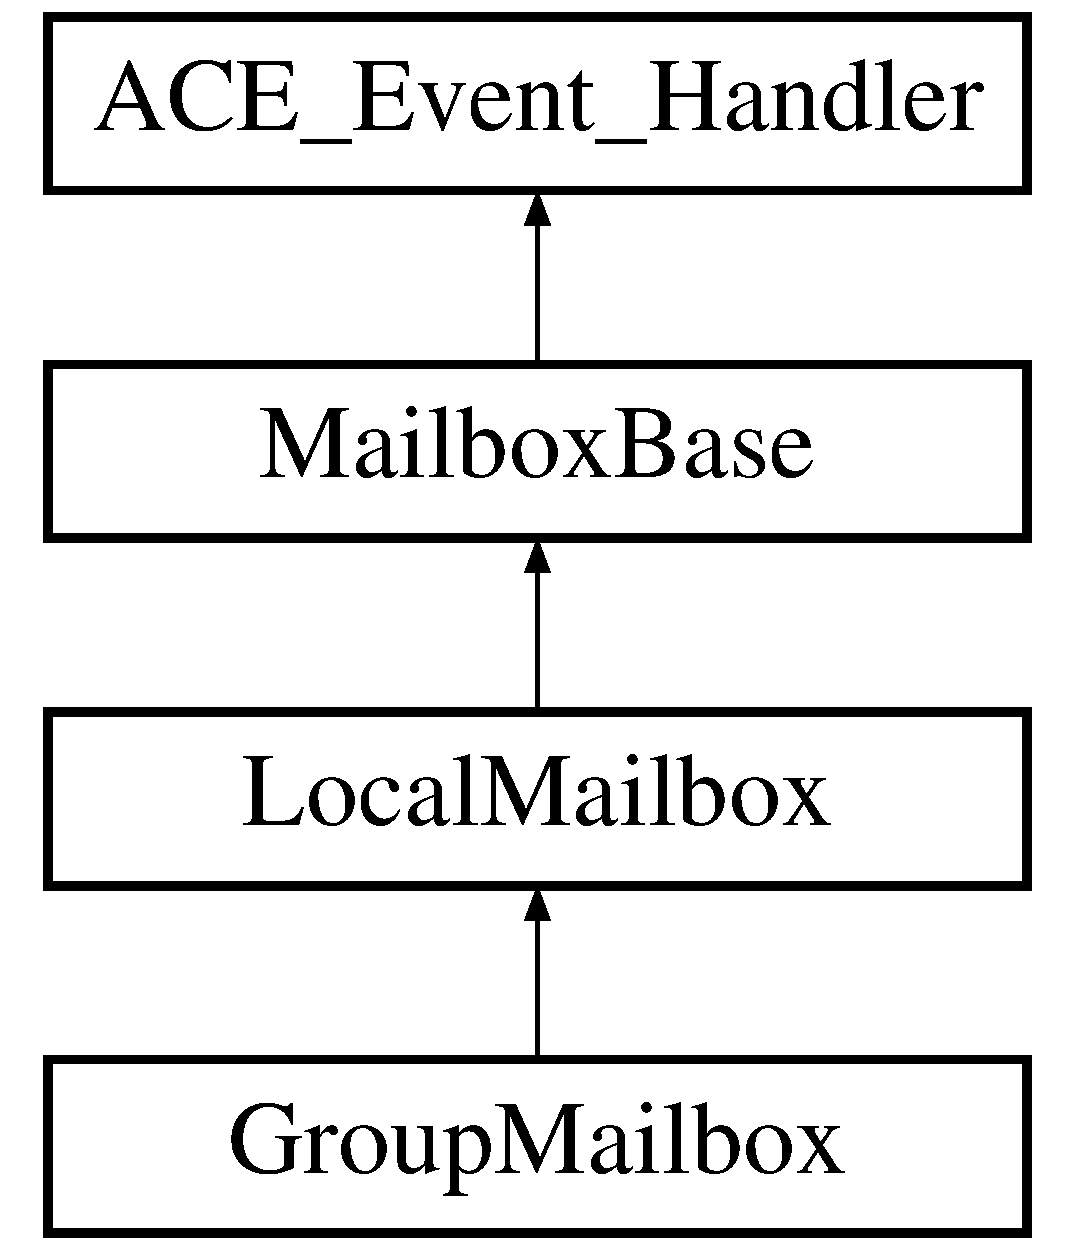
\includegraphics[height=4.000000cm]{classGroupMailbox}
\end{center}
\end{figure}
\subsection*{Public Member Functions}
\begin{DoxyCompactItemize}
\item 
virtual bool {\bf rename} (const {\bf Mailbox\+Address} \&new\+Group\+Address)
\item 
virtual int {\bf activate} ({\bf Mailbox\+Owner\+Handle} $\ast$mailbox\+Owner\+Handle)
\item 
virtual int {\bf deactivate} ({\bf Mailbox\+Owner\+Handle} $\ast$mailbox\+Owner\+Handle)
\item 
{\bf Mailbox\+Address} \& {\bf get\+Mailbox\+Address} ()
\item 
string {\bf to\+String} ()
\end{DoxyCompactItemize}
\subsection*{Static Public Member Functions}
\begin{DoxyCompactItemize}
\item 
static {\bf Mailbox\+Owner\+Handle} $\ast$ {\bf create\+Mailbox} (const {\bf Mailbox\+Address} \&group\+Address, unsigned int multicast\+Loopback\+Enabled=T\+R\+UE, unsigned int multicast\+T\+TL=1)
\end{DoxyCompactItemize}
\subsection*{Protected Member Functions}
\begin{DoxyCompactItemize}
\item 
{\bf Group\+Mailbox} (const {\bf Mailbox\+Address} \&group\+Address, unsigned int multicast\+Loopback\+Enabled\+\_\+, unsigned int multicast\+T\+T\+L\+\_\+)
\item 
virtual {\bf $\sim$\+Group\+Mailbox} ()
\end{DoxyCompactItemize}
\subsection*{Additional Inherited Members}


\subsection{Constructor \& Destructor Documentation}
\index{Group\+Mailbox@{Group\+Mailbox}!Group\+Mailbox@{Group\+Mailbox}}
\index{Group\+Mailbox@{Group\+Mailbox}!Group\+Mailbox@{Group\+Mailbox}}
\subsubsection[{Group\+Mailbox(const Mailbox\+Address \&group\+Address, unsigned int multicast\+Loopback\+Enabled\+\_\+, unsigned int multicast\+T\+T\+L\+\_\+)}]{\setlength{\rightskip}{0pt plus 5cm}Group\+Mailbox\+::\+Group\+Mailbox (
\begin{DoxyParamCaption}
\item[{const {\bf Mailbox\+Address} \&}]{group\+Address, }
\item[{unsigned int}]{multicast\+Loopback\+Enabled\+\_\+, }
\item[{unsigned int}]{multicast\+T\+T\+L\+\_\+}
\end{DoxyParamCaption}
)\hspace{0.3cm}{\ttfamily [protected]}}\label{classGroupMailbox_afc08cda431d7126f36019a936c0e663e}
Constructor -\/ protected so that applications cannot create their own mailboxes and must use the static \doxyref{create\+Mailbox()}{p.}{classGroupMailbox_a2c557e67a0ddc8518623d9cedcaa283f} method 

References Group\+Mailbox().



Referenced by Group\+Mailbox().

\index{Group\+Mailbox@{Group\+Mailbox}!````~Group\+Mailbox@{$\sim$\+Group\+Mailbox}}
\index{````~Group\+Mailbox@{$\sim$\+Group\+Mailbox}!Group\+Mailbox@{Group\+Mailbox}}
\subsubsection[{$\sim$\+Group\+Mailbox()}]{\setlength{\rightskip}{0pt plus 5cm}Group\+Mailbox\+::$\sim$\+Group\+Mailbox (
\begin{DoxyParamCaption}
{}
\end{DoxyParamCaption}
)\hspace{0.3cm}{\ttfamily [protected]}, {\ttfamily [virtual]}}\label{classGroupMailbox_aa5b47c0b7af860a1255691f4fa036a13}
Virtual Destructor. Protected since this is a reference counted object. 

References Mailbox\+Base\+::is\+Shutting\+Down\+\_\+.



\subsection{Member Function Documentation}
\index{Group\+Mailbox@{Group\+Mailbox}!activate@{activate}}
\index{activate@{activate}!Group\+Mailbox@{Group\+Mailbox}}
\subsubsection[{activate(\+Mailbox\+Owner\+Handle $\ast$mailbox\+Owner\+Handle)}]{\setlength{\rightskip}{0pt plus 5cm}int Group\+Mailbox\+::activate (
\begin{DoxyParamCaption}
\item[{{\bf Mailbox\+Owner\+Handle} $\ast$}]{mailbox\+Owner\+Handle}
\end{DoxyParamCaption}
)\hspace{0.3cm}{\ttfamily [virtual]}}\label{classGroupMailbox_a8376e1dfb4d001d6095ea3d7419765f6}
Activate the mailbox. For security, one must possess an Owner Handle in order to activate the mailbox and register it with the Lookup Service. 

Reimplemented from {\bf Local\+Mailbox} \doxyref{}{p.}{classLocalMailbox_a90a0b182b76f38934302d613c74b626f}.



References Local\+Mailbox\+::activate(), Local\+Mailbox\+::deactivate(), Mailbox\+Address\+::inet\+Address, and Mailbox\+Base\+::is\+Active().

\index{Group\+Mailbox@{Group\+Mailbox}!create\+Mailbox@{create\+Mailbox}}
\index{create\+Mailbox@{create\+Mailbox}!Group\+Mailbox@{Group\+Mailbox}}
\subsubsection[{create\+Mailbox(const Mailbox\+Address \&group\+Address, unsigned int multicast\+Loopback\+Enabled=\+T\+R\+U\+E, unsigned int multicast\+T\+T\+L=1)}]{\setlength{\rightskip}{0pt plus 5cm}{\bf Mailbox\+Owner\+Handle} $\ast$ Group\+Mailbox\+::create\+Mailbox (
\begin{DoxyParamCaption}
\item[{const {\bf Mailbox\+Address} \&}]{group\+Address, }
\item[{unsigned int}]{multicast\+Loopback\+Enabled = {\ttfamily TRUE}, }
\item[{unsigned int}]{multicast\+T\+TL = {\ttfamily 1}}
\end{DoxyParamCaption}
)\hspace{0.3cm}{\ttfamily [static]}}\label{classGroupMailbox_a2c557e67a0ddc8518623d9cedcaa283f}
Allows applications to create a mailbox and get a handle to it.

Since we do not want applications to have direct access to a mailbox object this method is provided. Applications that create mailboxes use this method to get a handle to their mailbox rather than have direct access. The handle returned is a owner handle which has all the privileges of the actual mailbox (get\+Message/post etc). This method creates the mailbox, activates it (which in turn registers it with the lookup service) and then creates an owner handle, acquires it and then returns that handle. Both the mailbox and the returned handle are created on the heap. 
\begin{DoxyParams}{Parameters}
{\em group\+Address} & source mailbox address that this mailbox will have \\
\hline
{\em multicast\+Loopback\+Enabled} & set to T\+R\+UE to enable multicast loopback \\
\hline
{\em multicast\+T\+TL} & If we experience problems with Multicast packets getting from one network to another, we need to probably change the T\+TL. By default, it is set to 1 to allow for only 1 hop (within the same subnet, routers will not forward). Also, setting to 0 will restrict to within the same host. \\
\hline
\end{DoxyParams}
\begin{DoxyReturn}{Returns}
pointer to a mailbox owner handle 
\end{DoxyReturn}


References Message\+Buffer\+::are\+Contents\+Processed(), Message\+Buffer\+::clear\+Buffer(), Thread\+Manager\+::create\+Thread(), Mailbox\+Base\+::debug\+Value\+\_\+, Message\+Buffer\+::get\+Buffer(), Message\+Base\+::get\+Message\+Id(), Message\+Base\+::get\+Source\+Address(), Mailbox\+Base\+::increment\+Received\+Count(), Mailbox\+Address\+::inet\+Address, Mailbox\+Address\+::location\+Type, Local\+Mailbox\+::post(), Message\+Factory\+::recreate\+Message\+From\+Buffer(), Mailbox\+Base\+::select\+Reactor\+\_\+, Message\+Buffer\+::set\+Insert\+Position(), Message\+Base\+::set\+Priority(), Local\+Mailbox\+::start\+Reactor(), and Message\+Base\+::to\+String().



Referenced by Discovery\+Manager\+::initialize().

\index{Group\+Mailbox@{Group\+Mailbox}!deactivate@{deactivate}}
\index{deactivate@{deactivate}!Group\+Mailbox@{Group\+Mailbox}}
\subsubsection[{deactivate(\+Mailbox\+Owner\+Handle $\ast$mailbox\+Owner\+Handle)}]{\setlength{\rightskip}{0pt plus 5cm}int Group\+Mailbox\+::deactivate (
\begin{DoxyParamCaption}
\item[{{\bf Mailbox\+Owner\+Handle} $\ast$}]{mailbox\+Owner\+Handle}
\end{DoxyParamCaption}
)\hspace{0.3cm}{\ttfamily [virtual]}}\label{classGroupMailbox_ae1aac18804e7584a90816ad6c840074d}
Deactivate the mailbox. For security, one must possess an Owner Handle in order to deactivate the mailbox and deregister it with the Lookup Service. 

Reimplemented from {\bf Local\+Mailbox} \doxyref{}{p.}{classLocalMailbox_a257122f75a72d9cbba8692cd1d8c431c}.



References Local\+Mailbox\+::deactivate(), and Mailbox\+Address\+::inet\+Address.

\index{Group\+Mailbox@{Group\+Mailbox}!get\+Mailbox\+Address@{get\+Mailbox\+Address}}
\index{get\+Mailbox\+Address@{get\+Mailbox\+Address}!Group\+Mailbox@{Group\+Mailbox}}
\subsubsection[{get\+Mailbox\+Address()}]{\setlength{\rightskip}{0pt plus 5cm}{\bf Mailbox\+Address} \& Group\+Mailbox\+::get\+Mailbox\+Address (
\begin{DoxyParamCaption}
{}
\end{DoxyParamCaption}
)\hspace{0.3cm}{\ttfamily [virtual]}}\label{classGroupMailbox_af3d24965817e7a326977ed01c59dfc7f}
Return the mailbox group address 

Implements {\bf Mailbox\+Base} \doxyref{}{p.}{classMailboxBase_ace28a599cdadf1afa99c94602eb7e4a6}.



References Mailbox\+Base\+::is\+Shutting\+Down\+\_\+.

\index{Group\+Mailbox@{Group\+Mailbox}!rename@{rename}}
\index{rename@{rename}!Group\+Mailbox@{Group\+Mailbox}}
\subsubsection[{rename(const Mailbox\+Address \&new\+Group\+Address)}]{\setlength{\rightskip}{0pt plus 5cm}bool Group\+Mailbox\+::rename (
\begin{DoxyParamCaption}
\item[{const {\bf Mailbox\+Address} \&}]{new\+Group\+Address}
\end{DoxyParamCaption}
)\hspace{0.3cm}{\ttfamily [virtual]}}\label{classGroupMailbox_a3f31059b9ea8924a92ef65b1afb44609}
Method to allow application to rename a mailbox\textquotesingle{}s group address.

T\+BD\+: What are the redundancy implications and usage here?? 

Reimplemented from {\bf Mailbox\+Base} \doxyref{}{p.}{classMailboxBase_a93bf1108b770d273af5c4282bdcdfe47}.

\index{Group\+Mailbox@{Group\+Mailbox}!to\+String@{to\+String}}
\index{to\+String@{to\+String}!Group\+Mailbox@{Group\+Mailbox}}
\subsubsection[{to\+String()}]{\setlength{\rightskip}{0pt plus 5cm}string Group\+Mailbox\+::to\+String (
\begin{DoxyParamCaption}
{}
\end{DoxyParamCaption}
)}\label{classGroupMailbox_a80922f6cd661a095be6e8840ad59240a}
String\textquotesingle{}ized debugging method \begin{DoxyReturn}{Returns}
string representation of the contents of this object 
\end{DoxyReturn}


The documentation for this class was generated from the following files\+:\begin{DoxyCompactItemize}
\item 
Group\+Mailbox.\+h\item 
Group\+Mailbox.\+cpp\end{DoxyCompactItemize}

\section{Group\+Mailbox\+Proxy Class Reference}
\label{classGroupMailboxProxy}\index{Group\+Mailbox\+Proxy@{Group\+Mailbox\+Proxy}}
Inheritance diagram for Group\+Mailbox\+Proxy\+:\begin{figure}[H]
\begin{center}
\leavevmode
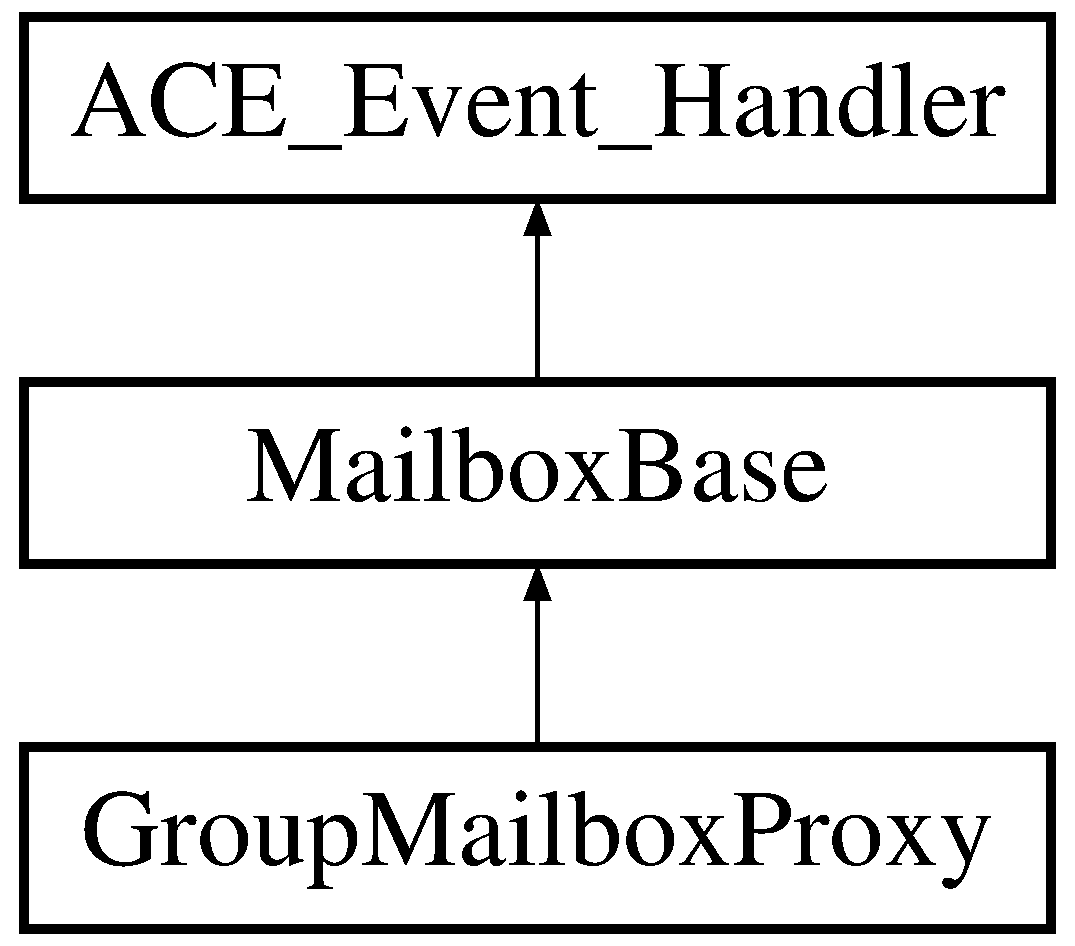
\includegraphics[height=3.000000cm]{classGroupMailboxProxy}
\end{center}
\end{figure}
\subsection*{Public Member Functions}
\begin{DoxyCompactItemize}
\item 
virtual int {\bf post} ({\bf Message\+Base} $\ast$message\+Ptr, const A\+C\+E\+\_\+\+Time\+\_\+\+Value $\ast$timeout=\&A\+C\+E\+\_\+\+Time\+\_\+\+Value\+::zero)
\item 
virtual int {\bf activate} ({\bf Mailbox\+Owner\+Handle} $\ast$mailbox\+Owner\+Handle)
\item 
virtual int {\bf deactivate} ({\bf Mailbox\+Owner\+Handle} $\ast$mailbox\+Owner\+Handle)
\item 
virtual const A\+C\+E\+\_\+\+Time\+\_\+\+Value \& {\bf get\+Post\+Default\+Timeout} ()
\item 
virtual int {\bf get\+Debug\+Value} ()
\item 
virtual void {\bf set\+Debug\+Value} (int debug\+Value)
\item 
{\bf Mailbox\+Address} \& {\bf get\+Mailbox\+Address} ()
\item 
string {\bf to\+String} ()
\end{DoxyCompactItemize}
\subsection*{Static Public Member Functions}
\begin{DoxyCompactItemize}
\item 
static {\bf Mailbox\+Owner\+Handle} $\ast$ {\bf create\+Mailbox} (const {\bf Mailbox\+Address} \&group\+Address, unsigned int multicast\+Loopback\+Enabled=T\+R\+UE, unsigned int multicast\+T\+TL=1)
\end{DoxyCompactItemize}
\subsection*{Protected Member Functions}
\begin{DoxyCompactItemize}
\item 
{\bf Group\+Mailbox\+Proxy} (const {\bf Mailbox\+Address} \&group\+Address, unsigned int multicast\+Loopback\+Enabled\+\_\+, unsigned int multicast\+T\+T\+L\+\_\+)
\item 
virtual {\bf $\sim$\+Group\+Mailbox\+Proxy} ()
\end{DoxyCompactItemize}
\subsection*{Additional Inherited Members}


\subsection{Constructor \& Destructor Documentation}
\index{Group\+Mailbox\+Proxy@{Group\+Mailbox\+Proxy}!Group\+Mailbox\+Proxy@{Group\+Mailbox\+Proxy}}
\index{Group\+Mailbox\+Proxy@{Group\+Mailbox\+Proxy}!Group\+Mailbox\+Proxy@{Group\+Mailbox\+Proxy}}
\subsubsection[{Group\+Mailbox\+Proxy(const Mailbox\+Address \&group\+Address, unsigned int multicast\+Loopback\+Enabled\+\_\+, unsigned int multicast\+T\+T\+L\+\_\+)}]{\setlength{\rightskip}{0pt plus 5cm}Group\+Mailbox\+Proxy\+::\+Group\+Mailbox\+Proxy (
\begin{DoxyParamCaption}
\item[{const {\bf Mailbox\+Address} \&}]{group\+Address, }
\item[{unsigned int}]{multicast\+Loopback\+Enabled\+\_\+, }
\item[{unsigned int}]{multicast\+T\+T\+L\+\_\+}
\end{DoxyParamCaption}
)\hspace{0.3cm}{\ttfamily [protected]}}\label{classGroupMailboxProxy_a2f5c3fead9b736b2a6b27eab848db595}
Constructor 

References O\+P\+M\+::create\+Pool(), Group\+Mailbox\+Proxy(), Message\+Buffer\+::initialize(), and Mailbox\+Base\+::is\+Proxy\+\_\+.



Referenced by Group\+Mailbox\+Proxy().

\index{Group\+Mailbox\+Proxy@{Group\+Mailbox\+Proxy}!````~Group\+Mailbox\+Proxy@{$\sim$\+Group\+Mailbox\+Proxy}}
\index{````~Group\+Mailbox\+Proxy@{$\sim$\+Group\+Mailbox\+Proxy}!Group\+Mailbox\+Proxy@{Group\+Mailbox\+Proxy}}
\subsubsection[{$\sim$\+Group\+Mailbox\+Proxy()}]{\setlength{\rightskip}{0pt plus 5cm}Group\+Mailbox\+Proxy\+::$\sim$\+Group\+Mailbox\+Proxy (
\begin{DoxyParamCaption}
{}
\end{DoxyParamCaption}
)\hspace{0.3cm}{\ttfamily [protected]}, {\ttfamily [virtual]}}\label{classGroupMailboxProxy_afeefad65497df7700a19bb2cdde7616c}
Virtual Destructor. Protected since this is a reference counted object. 

References Mailbox\+Base\+::is\+Shutting\+Down\+\_\+.



\subsection{Member Function Documentation}
\index{Group\+Mailbox\+Proxy@{Group\+Mailbox\+Proxy}!activate@{activate}}
\index{activate@{activate}!Group\+Mailbox\+Proxy@{Group\+Mailbox\+Proxy}}
\subsubsection[{activate(\+Mailbox\+Owner\+Handle $\ast$mailbox\+Owner\+Handle)}]{\setlength{\rightskip}{0pt plus 5cm}int Group\+Mailbox\+Proxy\+::activate (
\begin{DoxyParamCaption}
\item[{{\bf Mailbox\+Owner\+Handle} $\ast$}]{mailbox\+Owner\+Handle}
\end{DoxyParamCaption}
)\hspace{0.3cm}{\ttfamily [virtual]}}\label{classGroupMailboxProxy_a71886f6278da7cc6c0f36a647f259fcc}
Activate the mailbox. For security, one must possess an Owner Handle to activate the mailbox and register it with the Lookup Service. 

Reimplemented from {\bf Mailbox\+Base} \doxyref{}{p.}{classMailboxBase_a98c6c4736af9c084d5395d7a4303ec67}.



References Mailbox\+Address\+::inet\+Address, Mailbox\+Base\+::is\+Active(), Mailbox\+Lookup\+Service\+::register\+Mailbox(), and Mailbox\+Base\+::set\+Active().

\index{Group\+Mailbox\+Proxy@{Group\+Mailbox\+Proxy}!create\+Mailbox@{create\+Mailbox}}
\index{create\+Mailbox@{create\+Mailbox}!Group\+Mailbox\+Proxy@{Group\+Mailbox\+Proxy}}
\subsubsection[{create\+Mailbox(const Mailbox\+Address \&group\+Address, unsigned int multicast\+Loopback\+Enabled=\+T\+R\+U\+E, unsigned int multicast\+T\+T\+L=1)}]{\setlength{\rightskip}{0pt plus 5cm}{\bf Mailbox\+Owner\+Handle} $\ast$ Group\+Mailbox\+Proxy\+::create\+Mailbox (
\begin{DoxyParamCaption}
\item[{const {\bf Mailbox\+Address} \&}]{group\+Address, }
\item[{unsigned int}]{multicast\+Loopback\+Enabled = {\ttfamily TRUE}, }
\item[{unsigned int}]{multicast\+T\+TL = {\ttfamily 1}}
\end{DoxyParamCaption}
)\hspace{0.3cm}{\ttfamily [static]}}\label{classGroupMailboxProxy_a8069da98373d7faa9a702565bd5c2afe}
Allows applications to create a mailbox and get a handle to it.

Since we do not want applications to have direct access to a mailbox object this method is provided. Applications that create mailboxes use this method to get a handle to their mailbox rather than have direct access. The handle returned is a owner handle which has all the privileges of the actual mailbox (get\+Message/post etc). This method creates the mailbox, activates it (which in turn registers it with the lookup service) and then creates an owner handle, acquires it and then returns that handle. Both the mailbox and the returned handle are created on the heap. 
\begin{DoxyParams}{Parameters}
{\em group\+Address} & source mailbox address that this mailbox will have \\
\hline
{\em multicast\+Loopback\+Enabled} & set to T\+R\+UE to enable multicast loopback \\
\hline
{\em multicast\+T\+TL} & If we experience problems with Multicast packets getting from one network to another, we need to probably change the T\+TL. By default, it is set to 1 to allow for only 1 hop. (within the same subnet, routers will not forward). Also, setting to 0 will restrict to within the same host. \\
\hline
\end{DoxyParams}
\begin{DoxyReturn}{Returns}
pointer to a mailbox owner handle 
\end{DoxyReturn}


Referenced by Mailbox\+Lookup\+Service\+::find(), and Discovery\+Manager\+::process\+Mailbox().

\index{Group\+Mailbox\+Proxy@{Group\+Mailbox\+Proxy}!deactivate@{deactivate}}
\index{deactivate@{deactivate}!Group\+Mailbox\+Proxy@{Group\+Mailbox\+Proxy}}
\subsubsection[{deactivate(\+Mailbox\+Owner\+Handle $\ast$mailbox\+Owner\+Handle)}]{\setlength{\rightskip}{0pt plus 5cm}int Group\+Mailbox\+Proxy\+::deactivate (
\begin{DoxyParamCaption}
\item[{{\bf Mailbox\+Owner\+Handle} $\ast$}]{mailbox\+Owner\+Handle}
\end{DoxyParamCaption}
)\hspace{0.3cm}{\ttfamily [virtual]}}\label{classGroupMailboxProxy_a252cc906cddd4e76e533e6f3d059a418}
Deactivate the mailbox. For security, one must possess an Owner Handle to deactivate the mailbox and deregister it with the Lookup Service. 

Reimplemented from {\bf Mailbox\+Base} \doxyref{}{p.}{classMailboxBase_a14ba6bd7936f32ecb51763acb89c507c}.



References Mailbox\+Lookup\+Service\+::deregister\+Mailbox(), Mailbox\+Address\+::inet\+Address, Mailbox\+Base\+::is\+Active(), and Mailbox\+Base\+::set\+Active().

\index{Group\+Mailbox\+Proxy@{Group\+Mailbox\+Proxy}!get\+Debug\+Value@{get\+Debug\+Value}}
\index{get\+Debug\+Value@{get\+Debug\+Value}!Group\+Mailbox\+Proxy@{Group\+Mailbox\+Proxy}}
\subsubsection[{get\+Debug\+Value()}]{\setlength{\rightskip}{0pt plus 5cm}int Group\+Mailbox\+Proxy\+::get\+Debug\+Value (
\begin{DoxyParamCaption}
{}
\end{DoxyParamCaption}
)\hspace{0.3cm}{\ttfamily [virtual]}}\label{classGroupMailboxProxy_ac4e932a909a8c9e6822e0d6ce7fb6837}
Return the debug flag 

Implements {\bf Mailbox\+Base} \doxyref{}{p.}{classMailboxBase_af5d9b331f7cb55d27517def24cc16de6}.



References Mailbox\+Base\+::debug\+Value\+\_\+.

\index{Group\+Mailbox\+Proxy@{Group\+Mailbox\+Proxy}!get\+Mailbox\+Address@{get\+Mailbox\+Address}}
\index{get\+Mailbox\+Address@{get\+Mailbox\+Address}!Group\+Mailbox\+Proxy@{Group\+Mailbox\+Proxy}}
\subsubsection[{get\+Mailbox\+Address()}]{\setlength{\rightskip}{0pt plus 5cm}{\bf Mailbox\+Address} \& Group\+Mailbox\+Proxy\+::get\+Mailbox\+Address (
\begin{DoxyParamCaption}
{}
\end{DoxyParamCaption}
)\hspace{0.3cm}{\ttfamily [virtual]}}\label{classGroupMailboxProxy_a3c4059bb85aea2495e31146dfc868c87}
Return the mailbox group address 

Implements {\bf Mailbox\+Base} \doxyref{}{p.}{classMailboxBase_ace28a599cdadf1afa99c94602eb7e4a6}.

\index{Group\+Mailbox\+Proxy@{Group\+Mailbox\+Proxy}!get\+Post\+Default\+Timeout@{get\+Post\+Default\+Timeout}}
\index{get\+Post\+Default\+Timeout@{get\+Post\+Default\+Timeout}!Group\+Mailbox\+Proxy@{Group\+Mailbox\+Proxy}}
\subsubsection[{get\+Post\+Default\+Timeout()}]{\setlength{\rightskip}{0pt plus 5cm}const A\+C\+E\+\_\+\+Time\+\_\+\+Value \& Group\+Mailbox\+Proxy\+::get\+Post\+Default\+Timeout (
\begin{DoxyParamCaption}
{}
\end{DoxyParamCaption}
)\hspace{0.3cm}{\ttfamily [virtual]}}\label{classGroupMailboxProxy_ab693664971bfcf4123f5a39514a6d671}
Return the appropriate default timeout for the \doxyref{post()}{p.}{classGroupMailboxProxy_a753647fb4480c941e51e368d8bbf8a89} 

Implements {\bf Mailbox\+Base} \doxyref{}{p.}{classMailboxBase_a7e288209b5f7daf305f8a882a6b806c6}.

\index{Group\+Mailbox\+Proxy@{Group\+Mailbox\+Proxy}!post@{post}}
\index{post@{post}!Group\+Mailbox\+Proxy@{Group\+Mailbox\+Proxy}}
\subsubsection[{post(\+Message\+Base $\ast$message\+Ptr, const A\+C\+E\+\_\+\+Time\+\_\+\+Value $\ast$timeout=\&\+A\+C\+E\+\_\+\+Time\+\_\+\+Value\+::zero)}]{\setlength{\rightskip}{0pt plus 5cm}int Group\+Mailbox\+Proxy\+::post (
\begin{DoxyParamCaption}
\item[{{\bf Message\+Base} $\ast$}]{message\+Ptr, }
\item[{const A\+C\+E\+\_\+\+Time\+\_\+\+Value $\ast$}]{timeout = {\ttfamily \&ACE\+\_\+Time\+\_\+Value\+:\+:zero}}
\end{DoxyParamCaption}
)\hspace{0.3cm}{\ttfamily [virtual]}}\label{classGroupMailboxProxy_a753647fb4480c941e51e368d8bbf8a89}
Post a message to the group mailbox. Subclass implementations should examine the \char`\"{}active\+\_\+\char`\"{} state. Upon initial failure of the post, this proxy mailbox will close and re-\/open the socket and attempt to post the message again automatically. If the the repost fails, then E\+R\+R\+OR will be returned, and it becomes the responsibility of the application to retry the message after deleting the mailbox handle and performing \doxyref{Mailbox\+Lookup\+Service\+::find}{p.}{classMailboxLookupService_a04a96883cc551682e635924884e433ac} (which may return a redundant mate\textquotesingle{}s handle); or, the application can give up and delete the message off of the heap. \begin{DoxyReturn}{Returns}
E\+R\+R\+OR upon failure; OK otherwise. 
\end{DoxyReturn}


Implements {\bf Mailbox\+Base} \doxyref{}{p.}{classMailboxBase_a6ac15f4fcc8493e7cc1e79310f1129a7}.



References Mailbox\+Base\+::debug\+Value\+\_\+, Message\+Base\+::delete\+Message(), Message\+Base\+::get\+Message\+Id(), Message\+Base\+::get\+Priority(), Message\+Base\+::get\+Source\+Address(), Mailbox\+Base\+::increment\+Sent\+Count(), Mailbox\+Address\+::inet\+Address, Mailbox\+Base\+::is\+Active(), Message\+Base\+::serialize(), Message\+Base\+::to\+String(), and Mailbox\+Address\+::to\+String().

\index{Group\+Mailbox\+Proxy@{Group\+Mailbox\+Proxy}!set\+Debug\+Value@{set\+Debug\+Value}}
\index{set\+Debug\+Value@{set\+Debug\+Value}!Group\+Mailbox\+Proxy@{Group\+Mailbox\+Proxy}}
\subsubsection[{set\+Debug\+Value(int debug\+Value)}]{\setlength{\rightskip}{0pt plus 5cm}void Group\+Mailbox\+Proxy\+::set\+Debug\+Value (
\begin{DoxyParamCaption}
\item[{int}]{debug\+Value}
\end{DoxyParamCaption}
)\hspace{0.3cm}{\ttfamily [virtual]}}\label{classGroupMailboxProxy_aedebe98af0626f15e2c21620385c83c9}
Set the debug flag 

Implements {\bf Mailbox\+Base} \doxyref{}{p.}{classMailboxBase_a3be54965c1fafbc4de3d7e6087128a4f}.



References Mailbox\+Base\+::debug\+Value\+\_\+.

\index{Group\+Mailbox\+Proxy@{Group\+Mailbox\+Proxy}!to\+String@{to\+String}}
\index{to\+String@{to\+String}!Group\+Mailbox\+Proxy@{Group\+Mailbox\+Proxy}}
\subsubsection[{to\+String()}]{\setlength{\rightskip}{0pt plus 5cm}string Group\+Mailbox\+Proxy\+::to\+String (
\begin{DoxyParamCaption}
{}
\end{DoxyParamCaption}
)}\label{classGroupMailboxProxy_a87860bd36a07881e203ae308c810e4fa}
String\textquotesingle{}ized debugging method \begin{DoxyReturn}{Returns}
string representation of the contents of this object 
\end{DoxyReturn}


The documentation for this class was generated from the following files\+:\begin{DoxyCompactItemize}
\item 
Group\+Mailbox\+Proxy.\+h\item 
Group\+Mailbox\+Proxy.\+cpp\end{DoxyCompactItemize}

\section{Local\+Mailbox Class Reference}
\label{classLocalMailbox}\index{Local\+Mailbox@{Local\+Mailbox}}
Inheritance diagram for Local\+Mailbox\+:\begin{figure}[H]
\begin{center}
\leavevmode
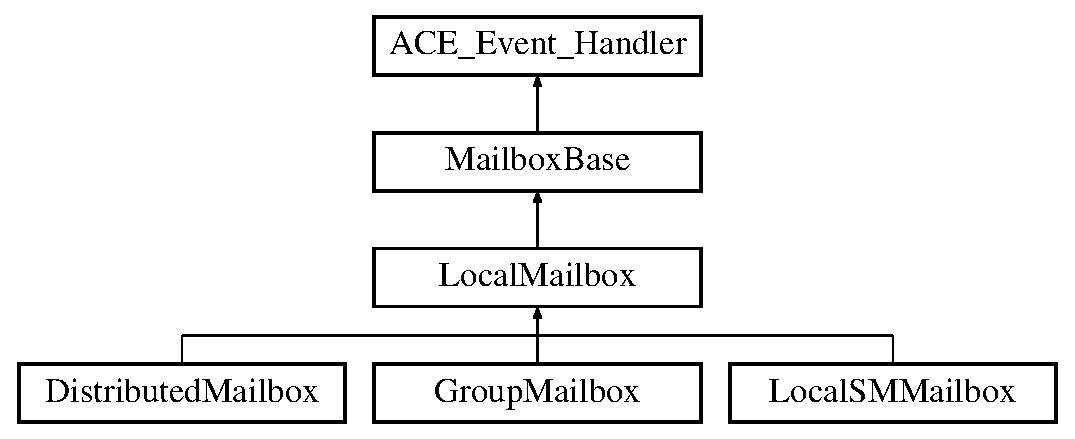
\includegraphics[height=4.000000cm]{classLocalMailbox}
\end{center}
\end{figure}
\subsection*{Public Member Functions}
\begin{DoxyCompactItemize}
\item 
virtual int {\bf activate} ({\bf Mailbox\+Owner\+Handle} $\ast$mailbox\+Owner\+Handle)
\item 
virtual int {\bf deactivate} ({\bf Mailbox\+Owner\+Handle} $\ast$mailbox\+Owner\+Handle)
\item 
virtual const A\+C\+E\+\_\+\+Time\+\_\+\+Value \& {\bf get\+Post\+Default\+Timeout} ()
\item 
virtual int {\bf post} ({\bf Message\+Base} $\ast$message\+Ptr, const A\+C\+E\+\_\+\+Time\+\_\+\+Value $\ast$timeout=\&A\+C\+E\+\_\+\+Time\+\_\+\+Value\+::zero)
\item 
virtual {\bf Message\+Base} $\ast$ {\bf get\+Message} (unsigned short timeout\+Value=0)
\item 
virtual {\bf Message\+Base} $\ast$ {\bf get\+Message\+Non\+Blocking} ()
\item 
virtual int {\bf get\+Debug\+Value} ()
\item 
virtual void {\bf set\+Debug\+Value} (int debug\+Value)
\item 
{\bf Mailbox\+Address} \& {\bf get\+Mailbox\+Address} ()
\end{DoxyCompactItemize}
\subsection*{Static Public Member Functions}
\begin{DoxyCompactItemize}
\item 
static {\bf Mailbox\+Owner\+Handle} $\ast$ {\bf create\+Mailbox} (const {\bf Mailbox\+Address} \&local\+Address)
\end{DoxyCompactItemize}
\subsection*{Protected Member Functions}
\begin{DoxyCompactItemize}
\item 
{\bf Local\+Mailbox} (const {\bf Mailbox\+Address} \&local\+Address)
\item 
virtual {\bf $\sim$\+Local\+Mailbox} ()
\end{DoxyCompactItemize}
\subsection*{Static Protected Member Functions}
\begin{DoxyCompactItemize}
\item 
static void {\bf start\+Reactor} (void $\ast$arg)
\end{DoxyCompactItemize}
\subsection*{Protected Attributes}
\begin{DoxyCompactItemize}
\item 
{\bf Mailbox\+Address} {\bf local\+Address\+\_\+}
\item 
A\+C\+E\+\_\+\+Message\+\_\+\+Queue$<$ A\+C\+E\+\_\+\+M\+T\+\_\+\+S\+Y\+N\+CH $>$ {\bf message\+Queue\+\_\+}
\end{DoxyCompactItemize}
\subsection*{Additional Inherited Members}


\subsection{Constructor \& Destructor Documentation}
\index{Local\+Mailbox@{Local\+Mailbox}!Local\+Mailbox@{Local\+Mailbox}}
\index{Local\+Mailbox@{Local\+Mailbox}!Local\+Mailbox@{Local\+Mailbox}}
\subsubsection[{Local\+Mailbox(const Mailbox\+Address \&local\+Address)}]{\setlength{\rightskip}{0pt plus 5cm}Local\+Mailbox\+::\+Local\+Mailbox (
\begin{DoxyParamCaption}
\item[{const {\bf Mailbox\+Address} \&}]{local\+Address}
\end{DoxyParamCaption}
)\hspace{0.3cm}{\ttfamily [protected]}}\label{classLocalMailbox_a8e36dd7afaac706c1aba94e4184cbcbe}
Default Constructor -\/ protected so that applications cannot create their own mailboxes and must use the static \doxyref{create\+Mailbox()}{p.}{classLocalMailbox_a42ed8ce49b76ecf0ccb4c3adde573af3} method 

References O\+P\+M\+::create\+Pool(), Message\+Block\+Wrapper\+::initialize(), and Local\+Mailbox().



Referenced by Local\+Mailbox().

\index{Local\+Mailbox@{Local\+Mailbox}!````~Local\+Mailbox@{$\sim$\+Local\+Mailbox}}
\index{````~Local\+Mailbox@{$\sim$\+Local\+Mailbox}!Local\+Mailbox@{Local\+Mailbox}}
\subsubsection[{$\sim$\+Local\+Mailbox()}]{\setlength{\rightskip}{0pt plus 5cm}Local\+Mailbox\+::$\sim$\+Local\+Mailbox (
\begin{DoxyParamCaption}
{}
\end{DoxyParamCaption}
)\hspace{0.3cm}{\ttfamily [protected]}, {\ttfamily [virtual]}}\label{classLocalMailbox_acf73630ae2b2eb0fa02743150c85205a}
Virtual Destructor. Protected since this is a reference counted object 

References Message\+Base\+::delete\+Message(), Message\+Base\+::is\+Poolable(), Mailbox\+Base\+::is\+Shutting\+Down\+\_\+, message\+Queue\+\_\+, and Mailbox\+Base\+::select\+Reactor\+\_\+.



\subsection{Member Function Documentation}
\index{Local\+Mailbox@{Local\+Mailbox}!activate@{activate}}
\index{activate@{activate}!Local\+Mailbox@{Local\+Mailbox}}
\subsubsection[{activate(\+Mailbox\+Owner\+Handle $\ast$mailbox\+Owner\+Handle)}]{\setlength{\rightskip}{0pt plus 5cm}int Local\+Mailbox\+::activate (
\begin{DoxyParamCaption}
\item[{{\bf Mailbox\+Owner\+Handle} $\ast$}]{mailbox\+Owner\+Handle}
\end{DoxyParamCaption}
)\hspace{0.3cm}{\ttfamily [virtual]}}\label{classLocalMailbox_a90a0b182b76f38934302d613c74b626f}
Activate the mailbox. For security, one must possess an Owner Handle to the mailbox in order to activate it and register it with the Lookup Service. 

Reimplemented from {\bf Mailbox\+Base} \doxyref{}{p.}{classMailboxBase_a98c6c4736af9c084d5395d7a4303ec67}.



Reimplemented in {\bf Group\+Mailbox} \doxyref{}{p.}{classGroupMailbox_a8376e1dfb4d001d6095ea3d7419765f6}, {\bf Distributed\+Mailbox} \doxyref{}{p.}{classDistributedMailbox_ace1358b217d0f0a52be4d32e3277c211}, and {\bf Local\+S\+M\+Mailbox} \doxyref{}{p.}{classLocalSMMailbox_a0a392404de9ca6224d0ed114c260b26a}.



References Mailbox\+Base\+::is\+Active(), message\+Queue\+\_\+, Mailbox\+Lookup\+Service\+::register\+Mailbox(), and Mailbox\+Base\+::set\+Active().



Referenced by Local\+S\+M\+Mailbox\+::activate(), Distributed\+Mailbox\+::activate(), Group\+Mailbox\+::activate(), and create\+Mailbox().

\index{Local\+Mailbox@{Local\+Mailbox}!create\+Mailbox@{create\+Mailbox}}
\index{create\+Mailbox@{create\+Mailbox}!Local\+Mailbox@{Local\+Mailbox}}
\subsubsection[{create\+Mailbox(const Mailbox\+Address \&local\+Address)}]{\setlength{\rightskip}{0pt plus 5cm}{\bf Mailbox\+Owner\+Handle} $\ast$ Local\+Mailbox\+::create\+Mailbox (
\begin{DoxyParamCaption}
\item[{const {\bf Mailbox\+Address} \&}]{local\+Address}
\end{DoxyParamCaption}
)\hspace{0.3cm}{\ttfamily [static]}}\label{classLocalMailbox_a42ed8ce49b76ecf0ccb4c3adde573af3}
Allows applications to create a mailbox and get a handle to it.

Since we do not want applications to have direct access to a mailbox object this method is provided. Applications that create mailboxes use this method to get a handle to their mailbox rather than have direct access. The handle returned is a owner handle which has all the privileges of the actual mailbox (get\+Message/post etc). This method creates the mailbox, activates it (which in turn registers it with the lookup service) and then creates an owner handle, acquires it and then returns that handle. Both the mailbox and the returned handle are created on the heap. 

References activate(), Thread\+Manager\+::create\+Thread(), Mailbox\+Address\+::default\+Unknown\+Inet\+Address\+\_\+, Mailbox\+Address\+::inet\+Address, Mailbox\+Address\+::location\+Type, Mailbox\+Address\+::mailbox\+Name, Mailbox\+Address\+::mailbox\+Type, Mailbox\+Address\+::neid, Mailbox\+Address\+::redundant\+Role, Mailbox\+Base\+::select\+Reactor\+\_\+, Mailbox\+Address\+::shelf\+Number, Mailbox\+Address\+::slot\+Number, and start\+Reactor().



Referenced by Process\+Manager\+::to\+String().

\index{Local\+Mailbox@{Local\+Mailbox}!deactivate@{deactivate}}
\index{deactivate@{deactivate}!Local\+Mailbox@{Local\+Mailbox}}
\subsubsection[{deactivate(\+Mailbox\+Owner\+Handle $\ast$mailbox\+Owner\+Handle)}]{\setlength{\rightskip}{0pt plus 5cm}int Local\+Mailbox\+::deactivate (
\begin{DoxyParamCaption}
\item[{{\bf Mailbox\+Owner\+Handle} $\ast$}]{mailbox\+Owner\+Handle}
\end{DoxyParamCaption}
)\hspace{0.3cm}{\ttfamily [virtual]}}\label{classLocalMailbox_a257122f75a72d9cbba8692cd1d8c431c}
Deactivate the mailbox. For security, one must possess an Owner Handle to the mailbox in order to deactivate it and deregister it with the Lookup Service. 

Reimplemented from {\bf Mailbox\+Base} \doxyref{}{p.}{classMailboxBase_a14ba6bd7936f32ecb51763acb89c507c}.



Reimplemented in {\bf Group\+Mailbox} \doxyref{}{p.}{classGroupMailbox_ae1aac18804e7584a90816ad6c840074d}, {\bf Distributed\+Mailbox} \doxyref{}{p.}{classDistributedMailbox_ab02bba7663485f4747afe81030737981}, and {\bf Local\+S\+M\+Mailbox} \doxyref{}{p.}{classLocalSMMailbox_ab78244c89f7fa411c40addc650906c3f}.



References Mailbox\+Lookup\+Service\+::deregister\+Mailbox(), Mailbox\+Base\+::is\+Active(), message\+Queue\+\_\+, and Mailbox\+Base\+::set\+Active().



Referenced by Distributed\+Mailbox\+::activate(), Group\+Mailbox\+::activate(), Local\+S\+M\+Mailbox\+::deactivate(), Distributed\+Mailbox\+::deactivate(), and Group\+Mailbox\+::deactivate().

\index{Local\+Mailbox@{Local\+Mailbox}!get\+Debug\+Value@{get\+Debug\+Value}}
\index{get\+Debug\+Value@{get\+Debug\+Value}!Local\+Mailbox@{Local\+Mailbox}}
\subsubsection[{get\+Debug\+Value()}]{\setlength{\rightskip}{0pt plus 5cm}int Local\+Mailbox\+::get\+Debug\+Value (
\begin{DoxyParamCaption}
{}
\end{DoxyParamCaption}
)\hspace{0.3cm}{\ttfamily [virtual]}}\label{classLocalMailbox_a51deb8f2ba82b15b81027880bd8ee931}
Returns the Debug flag value for this mailbox. 

Implements {\bf Mailbox\+Base} \doxyref{}{p.}{classMailboxBase_af5d9b331f7cb55d27517def24cc16de6}.



References Mailbox\+Base\+::debug\+Value\+\_\+.

\index{Local\+Mailbox@{Local\+Mailbox}!get\+Mailbox\+Address@{get\+Mailbox\+Address}}
\index{get\+Mailbox\+Address@{get\+Mailbox\+Address}!Local\+Mailbox@{Local\+Mailbox}}
\subsubsection[{get\+Mailbox\+Address()}]{\setlength{\rightskip}{0pt plus 5cm}{\bf Mailbox\+Address} \& Local\+Mailbox\+::get\+Mailbox\+Address (
\begin{DoxyParamCaption}
{}
\end{DoxyParamCaption}
)\hspace{0.3cm}{\ttfamily [virtual]}}\label{classLocalMailbox_a9524d5026b91c5f706ebdc22e58cfc76}
Return the mailbox address 

Implements {\bf Mailbox\+Base} \doxyref{}{p.}{classMailboxBase_ace28a599cdadf1afa99c94602eb7e4a6}.



Reimplemented in {\bf Local\+S\+M\+Mailbox} \doxyref{}{p.}{classLocalSMMailbox_a7dda4c081fcb30b3a653d13fb5530432}.



References local\+Address\+\_\+.

\index{Local\+Mailbox@{Local\+Mailbox}!get\+Message@{get\+Message}}
\index{get\+Message@{get\+Message}!Local\+Mailbox@{Local\+Mailbox}}
\subsubsection[{get\+Message(unsigned short timeout\+Value=0)}]{\setlength{\rightskip}{0pt plus 5cm}{\bf Message\+Base} $\ast$ Local\+Mailbox\+::get\+Message (
\begin{DoxyParamCaption}
\item[{unsigned short}]{timeout\+Value = {\ttfamily 0}}
\end{DoxyParamCaption}
)\hspace{0.3cm}{\ttfamily [virtual]}}\label{classLocalMailbox_a7e498769854f747d7c5a4b0996644259}
Will block until a message is available. Note that all non-\/\+Proxy Mailbox types use the \doxyref{Local\+Mailbox}{p.}{classLocalMailbox}\textquotesingle{}s get\+Message method to dequeue Msg\+Mgr messages. May return N\+U\+LL if no message available (if mailbox deactivated). 

Implements {\bf Mailbox\+Base} \doxyref{}{p.}{classMailboxBase_a3f6957be1bddd11487dec3b204f7ed82}.



References Mailbox\+Base\+::is\+Active(), and message\+Queue\+\_\+.

\index{Local\+Mailbox@{Local\+Mailbox}!get\+Message\+Non\+Blocking@{get\+Message\+Non\+Blocking}}
\index{get\+Message\+Non\+Blocking@{get\+Message\+Non\+Blocking}!Local\+Mailbox@{Local\+Mailbox}}
\subsubsection[{get\+Message\+Non\+Blocking()}]{\setlength{\rightskip}{0pt plus 5cm}{\bf Message\+Base} $\ast$ Local\+Mailbox\+::get\+Message\+Non\+Blocking (
\begin{DoxyParamCaption}
{}
\end{DoxyParamCaption}
)\hspace{0.3cm}{\ttfamily [virtual]}}\label{classLocalMailbox_a60cd9c185b9160ac9e12cca8c91b19a7}
Will not block until a message is available. 

If the application has a need to do non-\/blocking calls to get (or check to see if) messages pending on the mailbox queue, then the application needs to implement this call -\/instead-\/ of calling \doxyref{Mailbox\+Processor\+::process\+Mailbox()}{p.}{classMailboxProcessor_a464c9e9eb3df8dd68a72df4b37a61b0f}. If this is indeed the case, then the application will either need to implement the case switching on the Message Type -\/or-\/ implement the find for the \doxyref{Message\+Handler\+List}{p.}{classMessageHandlerList} (functor lookup). 

Note that all non-\/\+Proxy Mailbox types use the \doxyref{Local\+Mailbox}{p.}{classLocalMailbox}\textquotesingle{}s get\+Message method to dequeue Msg\+Mgr messages. \begin{DoxyReturn}{Returns}
N\+U\+LL if no message available (and if mailbox deactivated). 
\end{DoxyReturn}


Implements {\bf Mailbox\+Base} \doxyref{}{p.}{classMailboxBase_aad7075931168b7f353808461784a1c55}.



References Mailbox\+Base\+::is\+Active(), and message\+Queue\+\_\+.

\index{Local\+Mailbox@{Local\+Mailbox}!get\+Post\+Default\+Timeout@{get\+Post\+Default\+Timeout}}
\index{get\+Post\+Default\+Timeout@{get\+Post\+Default\+Timeout}!Local\+Mailbox@{Local\+Mailbox}}
\subsubsection[{get\+Post\+Default\+Timeout()}]{\setlength{\rightskip}{0pt plus 5cm}const A\+C\+E\+\_\+\+Time\+\_\+\+Value \& Local\+Mailbox\+::get\+Post\+Default\+Timeout (
\begin{DoxyParamCaption}
{}
\end{DoxyParamCaption}
)\hspace{0.3cm}{\ttfamily [virtual]}}\label{classLocalMailbox_a5e13fd0f4a2681099d5c4d10a5c6b0bc}
Return the post timeout 

Implements {\bf Mailbox\+Base} \doxyref{}{p.}{classMailboxBase_a7e288209b5f7daf305f8a882a6b806c6}.

\index{Local\+Mailbox@{Local\+Mailbox}!post@{post}}
\index{post@{post}!Local\+Mailbox@{Local\+Mailbox}}
\subsubsection[{post(\+Message\+Base $\ast$message\+Ptr, const A\+C\+E\+\_\+\+Time\+\_\+\+Value $\ast$timeout=\&\+A\+C\+E\+\_\+\+Time\+\_\+\+Value\+::zero)}]{\setlength{\rightskip}{0pt plus 5cm}int Local\+Mailbox\+::post (
\begin{DoxyParamCaption}
\item[{{\bf Message\+Base} $\ast$}]{message\+Ptr, }
\item[{const A\+C\+E\+\_\+\+Time\+\_\+\+Value $\ast$}]{timeout = {\ttfamily \&ACE\+\_\+Time\+\_\+Value\+:\+:zero}}
\end{DoxyParamCaption}
)\hspace{0.3cm}{\ttfamily [virtual]}}\label{classLocalMailbox_a9386ee91649cf2ced5133c2240e4799b}
Post a message to this mailbox. \begin{DoxyReturn}{Returns}
E\+R\+R\+OR for an error, OK otherwise. 
\end{DoxyReturn}


Implements {\bf Mailbox\+Base} \doxyref{}{p.}{classMailboxBase_a6ac15f4fcc8493e7cc1e79310f1129a7}.



References Message\+Block\+Wrapper\+::base(), Mailbox\+Base\+::debug\+Value\+\_\+, Message\+Base\+::get\+Message\+Id(), Message\+Base\+::get\+Priority(), Message\+Base\+::get\+Source\+Address(), Mailbox\+Base\+::is\+Active(), local\+Address\+\_\+, message\+Queue\+\_\+, Message\+Base\+::to\+String(), Mailbox\+Address\+::to\+String(), and Mailbox\+Base\+::to\+String().



Referenced by Distributed\+Mailbox\+::create\+Mailbox(), Group\+Mailbox\+::create\+Mailbox(), and Local\+S\+M\+Mailbox\+::get\+Mailbox\+Address().

\index{Local\+Mailbox@{Local\+Mailbox}!set\+Debug\+Value@{set\+Debug\+Value}}
\index{set\+Debug\+Value@{set\+Debug\+Value}!Local\+Mailbox@{Local\+Mailbox}}
\subsubsection[{set\+Debug\+Value(int debug\+Value)}]{\setlength{\rightskip}{0pt plus 5cm}void Local\+Mailbox\+::set\+Debug\+Value (
\begin{DoxyParamCaption}
\item[{int}]{debug\+Value}
\end{DoxyParamCaption}
)\hspace{0.3cm}{\ttfamily [virtual]}}\label{classLocalMailbox_aa66737102700c79d4e76b15202a0d9d9}
Sets the Debug flag value for this mailbox. 

Implements {\bf Mailbox\+Base} \doxyref{}{p.}{classMailboxBase_a3be54965c1fafbc4de3d7e6087128a4f}.



References Mailbox\+Base\+::debug\+Value\+\_\+.

\index{Local\+Mailbox@{Local\+Mailbox}!start\+Reactor@{start\+Reactor}}
\index{start\+Reactor@{start\+Reactor}!Local\+Mailbox@{Local\+Mailbox}}
\subsubsection[{start\+Reactor(void $\ast$arg)}]{\setlength{\rightskip}{0pt plus 5cm}void Local\+Mailbox\+::start\+Reactor (
\begin{DoxyParamCaption}
\item[{void $\ast$}]{arg}
\end{DoxyParamCaption}
)\hspace{0.3cm}{\ttfamily [static]}, {\ttfamily [protected]}}\label{classLocalMailbox_a8bbee22e03ae7d95637012f4ba37f221}
This static method is called in a new thread context to start the A\+CE Reactor event processing loop during mailbox activation. This will run the event loop until the $<$A\+C\+E\+\_\+\+Reactor\+::handle\+\_\+events$>$ or $<$A\+C\+E\+\_\+\+Reactor\+::alertable\+\_\+handle\+\_\+events$>$ methods returns -\/1, the $<$end\+\_\+reactor\+\_\+event\+\_\+loop$>$ method is invoked, or the $<$\+A\+C\+E\+\_\+\+Time\+\_\+\+Value$>$ expires. 
\begin{DoxyParams}{Parameters}
{\em arg} & Pointer to the reactor that we are going to start \\
\hline
\end{DoxyParams}


References Mailbox\+Base\+::is\+Shutting\+Down\+\_\+.



Referenced by Distributed\+Mailbox\+::create\+Mailbox(), Local\+S\+M\+Mailbox\+::create\+Mailbox(), Group\+Mailbox\+::create\+Mailbox(), and create\+Mailbox().



\subsection{Member Data Documentation}
\index{Local\+Mailbox@{Local\+Mailbox}!local\+Address\+\_\+@{local\+Address\+\_\+}}
\index{local\+Address\+\_\+@{local\+Address\+\_\+}!Local\+Mailbox@{Local\+Mailbox}}
\subsubsection[{local\+Address\+\_\+}]{\setlength{\rightskip}{0pt plus 5cm}{\bf Mailbox\+Address} Local\+Mailbox\+::local\+Address\+\_\+\hspace{0.3cm}{\ttfamily [protected]}}\label{classLocalMailbox_af39869ba036e70969ef725b1440b7155}
Address of this Mailbox 

Referenced by get\+Mailbox\+Address(), and post().

\index{Local\+Mailbox@{Local\+Mailbox}!message\+Queue\+\_\+@{message\+Queue\+\_\+}}
\index{message\+Queue\+\_\+@{message\+Queue\+\_\+}!Local\+Mailbox@{Local\+Mailbox}}
\subsubsection[{message\+Queue\+\_\+}]{\setlength{\rightskip}{0pt plus 5cm}A\+C\+E\+\_\+\+Message\+\_\+\+Queue$<$A\+C\+E\+\_\+\+M\+T\+\_\+\+S\+Y\+N\+CH$>$ Local\+Mailbox\+::message\+Queue\+\_\+\hspace{0.3cm}{\ttfamily [protected]}}\label{classLocalMailbox_a4544530bb185d8df5e95e5c82806180d}
Message queue for storing received messages 

Referenced by activate(), deactivate(), get\+Message(), get\+Message\+Non\+Blocking(), post(), and $\sim$\+Local\+Mailbox().



The documentation for this class was generated from the following files\+:\begin{DoxyCompactItemize}
\item 
Local\+Mailbox.\+h\item 
Local\+Mailbox.\+cpp\end{DoxyCompactItemize}

\section{Local\+S\+M\+Buffer Struct Reference}
\label{structLocalSMBuffer}\index{Local\+S\+M\+Buffer@{Local\+S\+M\+Buffer}}


{\ttfamily \#include $<$Local\+S\+M\+Buffer.\+h$>$}

Inheritance diagram for Local\+S\+M\+Buffer\+:\begin{figure}[H]
\begin{center}
\leavevmode
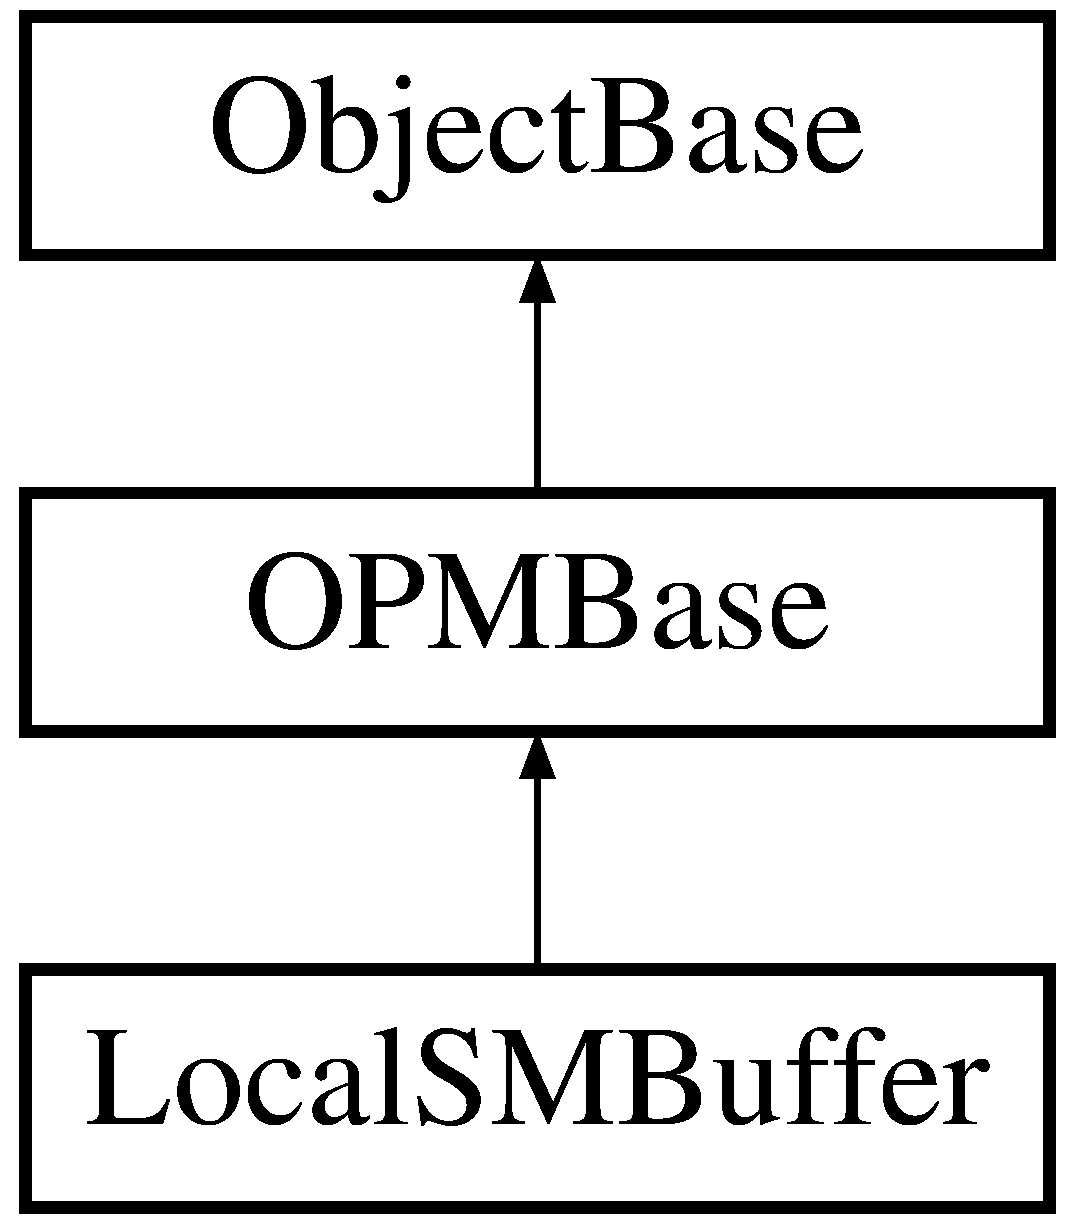
\includegraphics[height=3.000000cm]{structLocalSMBuffer}
\end{center}
\end{figure}
\subsection*{Public Member Functions}
\begin{DoxyCompactItemize}
\item 
{\bf Local\+S\+M\+Buffer} ()
\item 
virtual {\bf $\sim$\+Local\+S\+M\+Buffer} ()
\item 
{\bf Local\+S\+M\+Buffer} (const {\bf Local\+S\+M\+Buffer} \&rhs)
\item 
void {\bf reset} (void)
\item 
{\bf Local\+S\+M\+Buffer} \& {\bf operator=} (const {\bf Local\+S\+M\+Buffer} \&rhs)
\item 
void {\bf clean} ()
\end{DoxyCompactItemize}
\subsection*{Static Public Member Functions}
\begin{DoxyCompactItemize}
\item 
static {\bf O\+P\+M\+Base} $\ast$ {\bf initialize} (int initializer)
\end{DoxyCompactItemize}
\subsection*{Public Attributes}
\begin{DoxyCompactItemize}
\item 
unsigned char {\bf buffer} [M\+A\+X\+\_\+\+M\+E\+S\+S\+A\+G\+E\+\_\+\+L\+E\+N\+G\+TH]
\item 
A\+C\+E\+\_\+\+Based\+\_\+\+Pointer\+\_\+\+Basic$<$ unsigned char $>$ {\bf buffer\+PI}
\item 
unsigned int {\bf priority\+Level}
\item 
unsigned int {\bf version\+Number}
\item 
unsigned int {\bf buffer\+Length}
\end{DoxyCompactItemize}
\subsection*{Additional Inherited Members}


\subsection{Detailed Description}
\doxyref{Local\+S\+M\+Buffer}{p.}{structLocalSMBuffer} class is a wrapper for the \doxyref{Message\+Buffer}{p.}{classMessageBuffer}\textquotesingle{}s raw unsigned char buffer so that it can be passed through the shared memory queue with a position independent pointer. 

\doxyref{Local\+S\+M\+Buffer}{p.}{structLocalSMBuffer} assumes that all shared memory passed message will be of length M\+A\+X\+\_\+\+M\+E\+S\+S\+A\+G\+E\+\_\+\+L\+E\+N\+G\+TH. 

\begin{DoxyParagraph}{Author}
Stephen Horton
\end{DoxyParagraph}
\begin{DoxyParagraph}{Revision}
1
\end{DoxyParagraph}


\subsection{Constructor \& Destructor Documentation}
\index{Local\+S\+M\+Buffer@{Local\+S\+M\+Buffer}!Local\+S\+M\+Buffer@{Local\+S\+M\+Buffer}}
\index{Local\+S\+M\+Buffer@{Local\+S\+M\+Buffer}!Local\+S\+M\+Buffer@{Local\+S\+M\+Buffer}}
\subsubsection[{Local\+S\+M\+Buffer()}]{\setlength{\rightskip}{0pt plus 5cm}Local\+S\+M\+Buffer\+::\+Local\+S\+M\+Buffer (
\begin{DoxyParamCaption}
{}
\end{DoxyParamCaption}
)}\label{structLocalSMBuffer_aebea9c62356b753ff7e037b5475620ce}
Constructor 

References buffer, buffer\+PI, and O\+P\+M\+Base\+::set\+Object\+Type\+Str().



Referenced by initialize().

\index{Local\+S\+M\+Buffer@{Local\+S\+M\+Buffer}!````~Local\+S\+M\+Buffer@{$\sim$\+Local\+S\+M\+Buffer}}
\index{````~Local\+S\+M\+Buffer@{$\sim$\+Local\+S\+M\+Buffer}!Local\+S\+M\+Buffer@{Local\+S\+M\+Buffer}}
\subsubsection[{$\sim$\+Local\+S\+M\+Buffer()}]{\setlength{\rightskip}{0pt plus 5cm}Local\+S\+M\+Buffer\+::$\sim$\+Local\+S\+M\+Buffer (
\begin{DoxyParamCaption}
{}
\end{DoxyParamCaption}
)\hspace{0.3cm}{\ttfamily [virtual]}}\label{structLocalSMBuffer_a712b31e07ec33ab4842b478fa46d8b26}
Virtual Destructor \index{Local\+S\+M\+Buffer@{Local\+S\+M\+Buffer}!Local\+S\+M\+Buffer@{Local\+S\+M\+Buffer}}
\index{Local\+S\+M\+Buffer@{Local\+S\+M\+Buffer}!Local\+S\+M\+Buffer@{Local\+S\+M\+Buffer}}
\subsubsection[{Local\+S\+M\+Buffer(const Local\+S\+M\+Buffer \&rhs)}]{\setlength{\rightskip}{0pt plus 5cm}Local\+S\+M\+Buffer\+::\+Local\+S\+M\+Buffer (
\begin{DoxyParamCaption}
\item[{const {\bf Local\+S\+M\+Buffer} \&}]{rhs}
\end{DoxyParamCaption}
)}\label{structLocalSMBuffer_acac11fd463855f781a0c95799938644a}
Copy Constructor 

References buffer, and buffer\+PI.



\subsection{Member Function Documentation}
\index{Local\+S\+M\+Buffer@{Local\+S\+M\+Buffer}!clean@{clean}}
\index{clean@{clean}!Local\+S\+M\+Buffer@{Local\+S\+M\+Buffer}}
\subsubsection[{clean()}]{\setlength{\rightskip}{0pt plus 5cm}void Local\+S\+M\+Buffer\+::clean (
\begin{DoxyParamCaption}
{}
\end{DoxyParamCaption}
)\hspace{0.3cm}{\ttfamily [virtual]}}\label{structLocalSMBuffer_a5f30eb58740b77fc5aee9f39ae81f439}
\doxyref{O\+P\+M\+Base}{p.}{classOPMBase} clean method gets called when the object gets released back into its pool 

Implements {\bf O\+P\+M\+Base} \doxyref{}{p.}{classOPMBase_ad9ff8bb1ca9a1edfaaeb702f341713e9}.



References reset().

\index{Local\+S\+M\+Buffer@{Local\+S\+M\+Buffer}!initialize@{initialize}}
\index{initialize@{initialize}!Local\+S\+M\+Buffer@{Local\+S\+M\+Buffer}}
\subsubsection[{initialize(int initializer)}]{\setlength{\rightskip}{0pt plus 5cm}{\bf O\+P\+M\+Base} $\ast$ Local\+S\+M\+Buffer\+::initialize (
\begin{DoxyParamCaption}
\item[{int}]{initializer}
\end{DoxyParamCaption}
)\hspace{0.3cm}{\ttfamily [static]}}\label{structLocalSMBuffer_adb7c68f0c712c90866afc4bb96ff5431}
\doxyref{O\+P\+M\+Base}{p.}{classOPMBase} static initializer method for bootstrapping the objects 
\begin{DoxyParams}{Parameters}
{\em initializer} & Here the initializer will be the message buffer size to create. This assumes that we will have an \doxyref{O\+PM}{p.}{classOPM} object pool for each size of Message Buffer that we need. \\
\hline
\end{DoxyParams}


References Local\+S\+M\+Buffer().



Referenced by Local\+S\+M\+Mailbox\+Proxy\+::\+Local\+S\+M\+Mailbox\+Proxy().

\index{Local\+S\+M\+Buffer@{Local\+S\+M\+Buffer}!operator=@{operator=}}
\index{operator=@{operator=}!Local\+S\+M\+Buffer@{Local\+S\+M\+Buffer}}
\subsubsection[{operator=(const Local\+S\+M\+Buffer \&rhs)}]{\setlength{\rightskip}{0pt plus 5cm}{\bf Local\+S\+M\+Buffer} \& Local\+S\+M\+Buffer\+::operator= (
\begin{DoxyParamCaption}
\item[{const {\bf Local\+S\+M\+Buffer} \&}]{rhs}
\end{DoxyParamCaption}
)}\label{structLocalSMBuffer_a0109378a81314e9c95672da649361ecc}
Overloaded Assignment Operator 

References buffer, buffer\+Length, buffer\+PI, priority\+Level, and version\+Number.

\index{Local\+S\+M\+Buffer@{Local\+S\+M\+Buffer}!reset@{reset}}
\index{reset@{reset}!Local\+S\+M\+Buffer@{Local\+S\+M\+Buffer}}
\subsubsection[{reset(void)}]{\setlength{\rightskip}{0pt plus 5cm}void Local\+S\+M\+Buffer\+::reset (
\begin{DoxyParamCaption}
\item[{void}]{}
\end{DoxyParamCaption}
)}\label{structLocalSMBuffer_ab5c052d7b8d34c6c047c13c9ba3e98d2}
Reset all data members 

References buffer, buffer\+Length, buffer\+PI, priority\+Level, and version\+Number.



Referenced by clean(), and Local\+S\+M\+Mailbox\+::get\+Mailbox\+Address().



\subsection{Member Data Documentation}
\index{Local\+S\+M\+Buffer@{Local\+S\+M\+Buffer}!buffer@{buffer}}
\index{buffer@{buffer}!Local\+S\+M\+Buffer@{Local\+S\+M\+Buffer}}
\subsubsection[{buffer}]{\setlength{\rightskip}{0pt plus 5cm}unsigned char Local\+S\+M\+Buffer\+::buffer[M\+A\+X\+\_\+\+M\+E\+S\+S\+A\+G\+E\+\_\+\+L\+E\+N\+G\+TH]}\label{structLocalSMBuffer_a101f021c0b0c27ade21c5bbe8d737902}
Raw unsigned char message buffer from the \doxyref{Message\+Buffer}{p.}{classMessageBuffer} class 

Referenced by Local\+S\+M\+Buffer(), operator=(), Local\+S\+M\+Mailbox\+Proxy\+::post(), and reset().

\index{Local\+S\+M\+Buffer@{Local\+S\+M\+Buffer}!buffer\+Length@{buffer\+Length}}
\index{buffer\+Length@{buffer\+Length}!Local\+S\+M\+Buffer@{Local\+S\+M\+Buffer}}
\subsubsection[{buffer\+Length}]{\setlength{\rightskip}{0pt plus 5cm}unsigned int Local\+S\+M\+Buffer\+::buffer\+Length}\label{structLocalSMBuffer_ad85c8a65c52471694094027335f1caa2}
Buffer Length / sizeof the data 

Referenced by Local\+S\+M\+Mailbox\+::get\+Mailbox\+Address(), operator=(), Local\+S\+M\+Mailbox\+Proxy\+::post(), and reset().

\index{Local\+S\+M\+Buffer@{Local\+S\+M\+Buffer}!buffer\+PI@{buffer\+PI}}
\index{buffer\+PI@{buffer\+PI}!Local\+S\+M\+Buffer@{Local\+S\+M\+Buffer}}
\subsubsection[{buffer\+PI}]{\setlength{\rightskip}{0pt plus 5cm}A\+C\+E\+\_\+\+Based\+\_\+\+Pointer\+\_\+\+Basic$<$unsigned char$>$ Local\+S\+M\+Buffer\+::buffer\+PI}\label{structLocalSMBuffer_aef069192302bfc4cdd97fef25d052043}
Position Independent A\+CE Pointer to the log Message payload string. N\+O\+TE\+: there is no allocated memory here 

Referenced by Local\+S\+M\+Mailbox\+::get\+Mailbox\+Address(), Local\+S\+M\+Buffer(), operator=(), Local\+S\+M\+Mailbox\+Proxy\+::post(), and reset().

\index{Local\+S\+M\+Buffer@{Local\+S\+M\+Buffer}!priority\+Level@{priority\+Level}}
\index{priority\+Level@{priority\+Level}!Local\+S\+M\+Buffer@{Local\+S\+M\+Buffer}}
\subsubsection[{priority\+Level}]{\setlength{\rightskip}{0pt plus 5cm}unsigned int Local\+S\+M\+Buffer\+::priority\+Level}\label{structLocalSMBuffer_a1bd4f4c42c40b33227cb6e5de2e58910}
Priority Level of the Message. Default is 0. 

Referenced by Local\+S\+M\+Mailbox\+::get\+Mailbox\+Address(), operator=(), and reset().

\index{Local\+S\+M\+Buffer@{Local\+S\+M\+Buffer}!version\+Number@{version\+Number}}
\index{version\+Number@{version\+Number}!Local\+S\+M\+Buffer@{Local\+S\+M\+Buffer}}
\subsubsection[{version\+Number}]{\setlength{\rightskip}{0pt plus 5cm}unsigned int Local\+S\+M\+Buffer\+::version\+Number}\label{structLocalSMBuffer_aac7ac706c5f5aea8710115f6169ffc60}
Version number of the Message 

Referenced by operator=(), and reset().



The documentation for this struct was generated from the following files\+:\begin{DoxyCompactItemize}
\item 
Local\+S\+M\+Buffer.\+h\item 
Local\+S\+M\+Buffer.\+cpp\end{DoxyCompactItemize}

\section{Local\+S\+M\+Mailbox Class Reference}
\label{classLocalSMMailbox}\index{Local\+S\+M\+Mailbox@{Local\+S\+M\+Mailbox}}
Inheritance diagram for Local\+S\+M\+Mailbox\+:\begin{figure}[H]
\begin{center}
\leavevmode
\includegraphics[height=4.000000cm]{classLocalSMMailbox}
\end{center}
\end{figure}
\subsection*{Public Member Functions}
\begin{DoxyCompactItemize}
\item 
virtual int {\bf activate} ({\bf Mailbox\+Owner\+Handle} $\ast$mailbox\+Owner\+Handle)
\item 
virtual int {\bf deactivate} ({\bf Mailbox\+Owner\+Handle} $\ast$mailbox\+Owner\+Handle)
\item 
{\bf Mailbox\+Address} \& {\bf get\+Mailbox\+Address} ()
\item 
string {\bf to\+String} ()
\end{DoxyCompactItemize}
\subsection*{Static Public Member Functions}
\begin{DoxyCompactItemize}
\item 
static {\bf Mailbox\+Owner\+Handle} $\ast$ {\bf create\+Mailbox} (const {\bf Mailbox\+Address} \&local\+Address)
\end{DoxyCompactItemize}
\subsection*{Protected Member Functions}
\begin{DoxyCompactItemize}
\item 
{\bf Local\+S\+M\+Mailbox} (const {\bf Mailbox\+Address} \&local\+Address, const char $\ast$queue\+Name, const char $\ast$coordinating\+Mutex\+Name)
\item 
virtual {\bf $\sim$\+Local\+S\+M\+Mailbox} ()
\end{DoxyCompactItemize}
\subsection*{Additional Inherited Members}


\subsection{Constructor \& Destructor Documentation}
\index{Local\+S\+M\+Mailbox@{Local\+S\+M\+Mailbox}!Local\+S\+M\+Mailbox@{Local\+S\+M\+Mailbox}}
\index{Local\+S\+M\+Mailbox@{Local\+S\+M\+Mailbox}!Local\+S\+M\+Mailbox@{Local\+S\+M\+Mailbox}}
\subsubsection[{Local\+S\+M\+Mailbox(const Mailbox\+Address \&local\+Address, const char $\ast$queue\+Name, const char $\ast$coordinating\+Mutex\+Name)}]{\setlength{\rightskip}{0pt plus 5cm}Local\+S\+M\+Mailbox\+::\+Local\+S\+M\+Mailbox (
\begin{DoxyParamCaption}
\item[{const {\bf Mailbox\+Address} \&}]{local\+Address, }
\item[{const char $\ast$}]{queue\+Name, }
\item[{const char $\ast$}]{coordinating\+Mutex\+Name}
\end{DoxyParamCaption}
)\hspace{0.3cm}{\ttfamily [protected]}}\label{classLocalSMMailbox_a264d5de94f7b11b0040f31f4d4a5a2e1}
Constructor -\/ protected so that applications cannot create their own mailboxes and must use the static \doxyref{create\+Mailbox()}{p.}{classLocalSMMailbox_a68bdc7dd5d5b5cec2b8a1b86c2a02d07} method 

References Mailbox\+Base\+::debug\+Value\+\_\+, Local\+S\+M\+Mailbox(), and Mailbox\+Address\+::to\+String().



Referenced by Local\+S\+M\+Mailbox().

\index{Local\+S\+M\+Mailbox@{Local\+S\+M\+Mailbox}!````~Local\+S\+M\+Mailbox@{$\sim$\+Local\+S\+M\+Mailbox}}
\index{````~Local\+S\+M\+Mailbox@{$\sim$\+Local\+S\+M\+Mailbox}!Local\+S\+M\+Mailbox@{Local\+S\+M\+Mailbox}}
\subsubsection[{$\sim$\+Local\+S\+M\+Mailbox()}]{\setlength{\rightskip}{0pt plus 5cm}Local\+S\+M\+Mailbox\+::$\sim$\+Local\+S\+M\+Mailbox (
\begin{DoxyParamCaption}
{}
\end{DoxyParamCaption}
)\hspace{0.3cm}{\ttfamily [protected]}, {\ttfamily [virtual]}}\label{classLocalSMMailbox_a25bdecf4ace66c7fcdde4e645ab4ba39}
Virtual Destructor. Protected since this is a reference counted object. 

References Mailbox\+Base\+::is\+Shutting\+Down\+\_\+.



\subsection{Member Function Documentation}
\index{Local\+S\+M\+Mailbox@{Local\+S\+M\+Mailbox}!activate@{activate}}
\index{activate@{activate}!Local\+S\+M\+Mailbox@{Local\+S\+M\+Mailbox}}
\subsubsection[{activate(\+Mailbox\+Owner\+Handle $\ast$mailbox\+Owner\+Handle)}]{\setlength{\rightskip}{0pt plus 5cm}int Local\+S\+M\+Mailbox\+::activate (
\begin{DoxyParamCaption}
\item[{{\bf Mailbox\+Owner\+Handle} $\ast$}]{mailbox\+Owner\+Handle}
\end{DoxyParamCaption}
)\hspace{0.3cm}{\ttfamily [virtual]}}\label{classLocalSMMailbox_a0a392404de9ca6224d0ed114c260b26a}
Activate the mailbox. For security, one must possess an Owner handle to activate the mailbox and register it with the Lookup Service. 

Reimplemented from {\bf Local\+Mailbox} \doxyref{}{p.}{classLocalMailbox_a90a0b182b76f38934302d613c74b626f}.



References Local\+Mailbox\+::activate(), Thread\+Manager\+::create\+Thread(), and Mailbox\+Base\+::is\+Active().

\index{Local\+S\+M\+Mailbox@{Local\+S\+M\+Mailbox}!create\+Mailbox@{create\+Mailbox}}
\index{create\+Mailbox@{create\+Mailbox}!Local\+S\+M\+Mailbox@{Local\+S\+M\+Mailbox}}
\subsubsection[{create\+Mailbox(const Mailbox\+Address \&local\+Address)}]{\setlength{\rightskip}{0pt plus 5cm}{\bf Mailbox\+Owner\+Handle} $\ast$ Local\+S\+M\+Mailbox\+::create\+Mailbox (
\begin{DoxyParamCaption}
\item[{const {\bf Mailbox\+Address} \&}]{local\+Address}
\end{DoxyParamCaption}
)\hspace{0.3cm}{\ttfamily [static]}}\label{classLocalSMMailbox_a68bdc7dd5d5b5cec2b8a1b86c2a02d07}
Allows applications to create a mailbox and get a handle to it.

Since we do not want applications to have direct access to a mailbox object this method is provided. Applications that create mailboxes use this method to get a handle to their mailbox rather than have direct access. The handle returned is a owner handle which has all the privileges of the actual mailbox (get\+Message/post etc). This method creates the mailbox, activates it (which in turn registers it with the lookup service) and then creates an owner handle, acquires it and then returns that handle. Both the mailbox and the returned handle are created on the heap. 

References Thread\+Manager\+::create\+Thread(), Mailbox\+Address\+::location\+Type, Mailbox\+Address\+::mailbox\+Name, Mailbox\+Base\+::select\+Reactor\+\_\+, Local\+S\+M\+Mailbox\+Queue\+::setup\+Queue(), and Local\+Mailbox\+::start\+Reactor().

\index{Local\+S\+M\+Mailbox@{Local\+S\+M\+Mailbox}!deactivate@{deactivate}}
\index{deactivate@{deactivate}!Local\+S\+M\+Mailbox@{Local\+S\+M\+Mailbox}}
\subsubsection[{deactivate(\+Mailbox\+Owner\+Handle $\ast$mailbox\+Owner\+Handle)}]{\setlength{\rightskip}{0pt plus 5cm}int Local\+S\+M\+Mailbox\+::deactivate (
\begin{DoxyParamCaption}
\item[{{\bf Mailbox\+Owner\+Handle} $\ast$}]{mailbox\+Owner\+Handle}
\end{DoxyParamCaption}
)\hspace{0.3cm}{\ttfamily [virtual]}}\label{classLocalSMMailbox_ab78244c89f7fa411c40addc650906c3f}
Deactivate the mailbox. For security, one must possess an Owner handle to deactivate the mailbox and deregister it with the Lookup Service. 

Reimplemented from {\bf Local\+Mailbox} \doxyref{}{p.}{classLocalMailbox_a257122f75a72d9cbba8692cd1d8c431c}.



References Local\+Mailbox\+::deactivate().

\index{Local\+S\+M\+Mailbox@{Local\+S\+M\+Mailbox}!get\+Mailbox\+Address@{get\+Mailbox\+Address}}
\index{get\+Mailbox\+Address@{get\+Mailbox\+Address}!Local\+S\+M\+Mailbox@{Local\+S\+M\+Mailbox}}
\subsubsection[{get\+Mailbox\+Address()}]{\setlength{\rightskip}{0pt plus 5cm}{\bf Mailbox\+Address} \& Local\+S\+M\+Mailbox\+::get\+Mailbox\+Address (
\begin{DoxyParamCaption}
{}
\end{DoxyParamCaption}
)\hspace{0.3cm}{\ttfamily [virtual]}}\label{classLocalSMMailbox_a7dda4c081fcb30b3a653d13fb5530432}
Return the mailbox address 

Reimplemented from {\bf Local\+Mailbox} \doxyref{}{p.}{classLocalMailbox_a9524d5026b91c5f706ebdc22e58cfc76}.



References Message\+Buffer\+::assign\+Buffer(), Local\+S\+M\+Buffer\+::buffer\+Length, Local\+S\+M\+Buffer\+::buffer\+PI, Message\+Buffer\+::clear\+Buffer(), Mailbox\+Base\+::debug\+Value\+\_\+, Local\+S\+M\+Mailbox\+Queue\+::dequeue\+Message(), Message\+Base\+::get\+Message\+Id(), Message\+Base\+::get\+Source\+Address(), Mailbox\+Base\+::increment\+Received\+Count(), Mailbox\+Address\+::inet\+Address, Mailbox\+Base\+::is\+Active(), Local\+S\+M\+Mailbox\+Queue\+::is\+Empty(), Local\+Mailbox\+::post(), Local\+S\+M\+Buffer\+::priority\+Level, Message\+Factory\+::recreate\+Message\+From\+Buffer(), Local\+S\+M\+Buffer\+::reset(), Message\+Buffer\+::set\+Insert\+Position(), Message\+Base\+::set\+Priority(), and Message\+Base\+::to\+String().

\index{Local\+S\+M\+Mailbox@{Local\+S\+M\+Mailbox}!to\+String@{to\+String}}
\index{to\+String@{to\+String}!Local\+S\+M\+Mailbox@{Local\+S\+M\+Mailbox}}
\subsubsection[{to\+String()}]{\setlength{\rightskip}{0pt plus 5cm}string Local\+S\+M\+Mailbox\+::to\+String (
\begin{DoxyParamCaption}
{}
\end{DoxyParamCaption}
)}\label{classLocalSMMailbox_ae7c8cd2fea80619bfdb51708efdfa41e}
String\textquotesingle{}ized debugging method \begin{DoxyReturn}{Returns}
string representation of the contents of this object 
\end{DoxyReturn}


The documentation for this class was generated from the following files\+:\begin{DoxyCompactItemize}
\item 
Local\+S\+M\+Mailbox.\+h\item 
Local\+S\+M\+Mailbox.\+cpp\end{DoxyCompactItemize}

\section{Local\+S\+M\+Mailbox\+Proxy Class Reference}
\label{classLocalSMMailboxProxy}\index{Local\+S\+M\+Mailbox\+Proxy@{Local\+S\+M\+Mailbox\+Proxy}}
Inheritance diagram for Local\+S\+M\+Mailbox\+Proxy\+:\begin{figure}[H]
\begin{center}
\leavevmode
\includegraphics[height=3.000000cm]{classLocalSMMailboxProxy}
\end{center}
\end{figure}
\subsection*{Public Member Functions}
\begin{DoxyCompactItemize}
\item 
virtual int {\bf post} ({\bf Message\+Base} $\ast$message\+Ptr, const A\+C\+E\+\_\+\+Time\+\_\+\+Value $\ast$timeout=\&A\+C\+E\+\_\+\+Time\+\_\+\+Value\+::zero)
\item 
virtual int {\bf activate} ({\bf Mailbox\+Owner\+Handle} $\ast$mailbox\+Owner\+Handle)
\item 
virtual int {\bf deactivate} ({\bf Mailbox\+Owner\+Handle} $\ast$mailbox\+Owner\+Handle)
\item 
virtual const A\+C\+E\+\_\+\+Time\+\_\+\+Value \& {\bf get\+Post\+Default\+Timeout} ()
\item 
virtual int {\bf get\+Debug\+Value} ()
\item 
virtual void {\bf set\+Debug\+Value} (int debug\+Value)
\item 
{\bf Mailbox\+Address} \& {\bf get\+Mailbox\+Address} ()
\item 
string {\bf to\+String} ()
\end{DoxyCompactItemize}
\subsection*{Static Public Member Functions}
\begin{DoxyCompactItemize}
\item 
static {\bf Mailbox\+Owner\+Handle} $\ast$ {\bf create\+Mailbox} (const {\bf Mailbox\+Address} \&local\+Address)
\end{DoxyCompactItemize}
\subsection*{Protected Member Functions}
\begin{DoxyCompactItemize}
\item 
{\bf Local\+S\+M\+Mailbox\+Proxy} (const {\bf Mailbox\+Address} \&local\+Address, const char $\ast$queue\+Name, const char $\ast$coordinating\+Mutex\+Name)
\item 
virtual {\bf $\sim$\+Local\+S\+M\+Mailbox\+Proxy} ()
\end{DoxyCompactItemize}
\subsection*{Additional Inherited Members}


\subsection{Constructor \& Destructor Documentation}
\index{Local\+S\+M\+Mailbox\+Proxy@{Local\+S\+M\+Mailbox\+Proxy}!Local\+S\+M\+Mailbox\+Proxy@{Local\+S\+M\+Mailbox\+Proxy}}
\index{Local\+S\+M\+Mailbox\+Proxy@{Local\+S\+M\+Mailbox\+Proxy}!Local\+S\+M\+Mailbox\+Proxy@{Local\+S\+M\+Mailbox\+Proxy}}
\subsubsection[{Local\+S\+M\+Mailbox\+Proxy(const Mailbox\+Address \&local\+Address, const char $\ast$queue\+Name, const char $\ast$coordinating\+Mutex\+Name)}]{\setlength{\rightskip}{0pt plus 5cm}Local\+S\+M\+Mailbox\+Proxy\+::\+Local\+S\+M\+Mailbox\+Proxy (
\begin{DoxyParamCaption}
\item[{const {\bf Mailbox\+Address} \&}]{local\+Address, }
\item[{const char $\ast$}]{queue\+Name, }
\item[{const char $\ast$}]{coordinating\+Mutex\+Name}
\end{DoxyParamCaption}
)\hspace{0.3cm}{\ttfamily [protected]}}\label{classLocalSMMailboxProxy_a292cf4c04d662f5a332e12be29795a33}
Constructor 

References O\+P\+M\+::create\+Pool(), Message\+Buffer\+::initialize(), Local\+S\+M\+Buffer\+::initialize(), Mailbox\+Base\+::is\+Proxy\+\_\+, Local\+S\+M\+Mailbox\+Proxy(), and Mailbox\+Address\+::to\+String().



Referenced by Local\+S\+M\+Mailbox\+Proxy().

\index{Local\+S\+M\+Mailbox\+Proxy@{Local\+S\+M\+Mailbox\+Proxy}!````~Local\+S\+M\+Mailbox\+Proxy@{$\sim$\+Local\+S\+M\+Mailbox\+Proxy}}
\index{````~Local\+S\+M\+Mailbox\+Proxy@{$\sim$\+Local\+S\+M\+Mailbox\+Proxy}!Local\+S\+M\+Mailbox\+Proxy@{Local\+S\+M\+Mailbox\+Proxy}}
\subsubsection[{$\sim$\+Local\+S\+M\+Mailbox\+Proxy()}]{\setlength{\rightskip}{0pt plus 5cm}Local\+S\+M\+Mailbox\+Proxy\+::$\sim$\+Local\+S\+M\+Mailbox\+Proxy (
\begin{DoxyParamCaption}
{}
\end{DoxyParamCaption}
)\hspace{0.3cm}{\ttfamily [protected]}, {\ttfamily [virtual]}}\label{classLocalSMMailboxProxy_a177c1822f872f7cd9ddc188ccbf60a32}
Virtual Destructor. Protected since this is a reference counted object. 

References Mailbox\+Base\+::is\+Shutting\+Down\+\_\+.



\subsection{Member Function Documentation}
\index{Local\+S\+M\+Mailbox\+Proxy@{Local\+S\+M\+Mailbox\+Proxy}!activate@{activate}}
\index{activate@{activate}!Local\+S\+M\+Mailbox\+Proxy@{Local\+S\+M\+Mailbox\+Proxy}}
\subsubsection[{activate(\+Mailbox\+Owner\+Handle $\ast$mailbox\+Owner\+Handle)}]{\setlength{\rightskip}{0pt plus 5cm}int Local\+S\+M\+Mailbox\+Proxy\+::activate (
\begin{DoxyParamCaption}
\item[{{\bf Mailbox\+Owner\+Handle} $\ast$}]{mailbox\+Owner\+Handle}
\end{DoxyParamCaption}
)\hspace{0.3cm}{\ttfamily [virtual]}}\label{classLocalSMMailboxProxy_a472b03750fd8ef24db5c42b77c4dc0b8}
Activate the mailbox. Here, activate always returns true since all we have to do is map into shared memory. It returns true regardless if the Shared Memory Queue already exists in shared memory or if we had to create it (meaning we are enqueuing, but no one is listening). 

For security, one must possess an Owner Handle to activate the mailbox and register it with the Lookup Service. 

Reimplemented from {\bf Mailbox\+Base} \doxyref{}{p.}{classMailboxBase_a98c6c4736af9c084d5395d7a4303ec67}.



References Mailbox\+Base\+::is\+Active(), Mailbox\+Lookup\+Service\+::register\+Mailbox(), and Mailbox\+Base\+::set\+Active().

\index{Local\+S\+M\+Mailbox\+Proxy@{Local\+S\+M\+Mailbox\+Proxy}!create\+Mailbox@{create\+Mailbox}}
\index{create\+Mailbox@{create\+Mailbox}!Local\+S\+M\+Mailbox\+Proxy@{Local\+S\+M\+Mailbox\+Proxy}}
\subsubsection[{create\+Mailbox(const Mailbox\+Address \&local\+Address)}]{\setlength{\rightskip}{0pt plus 5cm}{\bf Mailbox\+Owner\+Handle} $\ast$ Local\+S\+M\+Mailbox\+Proxy\+::create\+Mailbox (
\begin{DoxyParamCaption}
\item[{const {\bf Mailbox\+Address} \&}]{local\+Address}
\end{DoxyParamCaption}
)\hspace{0.3cm}{\ttfamily [static]}}\label{classLocalSMMailboxProxy_aa98933b0c03489e5048fb9b050005acb}
Allows applications to create a mailbox and get a handle to it.

Since we do not want applications to have direct access to a mailbox object this method is provided. Applications that create mailboxes use this method to get a handle to their mailbox rather than have direct access. The handle returned is a owner handle which has all the privileges of the actual mailbox (get\+Message/post etc). This method creates the mailbox, activates it (which in turn registers it with the lookup service) and then creates an owner handle, acquires it and then returns that handle. Both the mailbox and the returned handle are created on the heap. 

References Mailbox\+Address\+::mailbox\+Name, and Local\+S\+M\+Mailbox\+Queue\+::setup\+Queue().



Referenced by Mailbox\+Lookup\+Service\+::find().

\index{Local\+S\+M\+Mailbox\+Proxy@{Local\+S\+M\+Mailbox\+Proxy}!deactivate@{deactivate}}
\index{deactivate@{deactivate}!Local\+S\+M\+Mailbox\+Proxy@{Local\+S\+M\+Mailbox\+Proxy}}
\subsubsection[{deactivate(\+Mailbox\+Owner\+Handle $\ast$mailbox\+Owner\+Handle)}]{\setlength{\rightskip}{0pt plus 5cm}int Local\+S\+M\+Mailbox\+Proxy\+::deactivate (
\begin{DoxyParamCaption}
\item[{{\bf Mailbox\+Owner\+Handle} $\ast$}]{mailbox\+Owner\+Handle}
\end{DoxyParamCaption}
)\hspace{0.3cm}{\ttfamily [virtual]}}\label{classLocalSMMailboxProxy_afb58d2be281db9d6e32503f20d56c502}
Deactivate the mailbox. For security, one must possess an Owner Handle to deactivate the mailbox and deregister it with the Lookup Service. 

Reimplemented from {\bf Mailbox\+Base} \doxyref{}{p.}{classMailboxBase_a14ba6bd7936f32ecb51763acb89c507c}.



References Mailbox\+Lookup\+Service\+::deregister\+Mailbox(), Mailbox\+Base\+::is\+Active(), and Mailbox\+Base\+::set\+Active().

\index{Local\+S\+M\+Mailbox\+Proxy@{Local\+S\+M\+Mailbox\+Proxy}!get\+Debug\+Value@{get\+Debug\+Value}}
\index{get\+Debug\+Value@{get\+Debug\+Value}!Local\+S\+M\+Mailbox\+Proxy@{Local\+S\+M\+Mailbox\+Proxy}}
\subsubsection[{get\+Debug\+Value()}]{\setlength{\rightskip}{0pt plus 5cm}int Local\+S\+M\+Mailbox\+Proxy\+::get\+Debug\+Value (
\begin{DoxyParamCaption}
{}
\end{DoxyParamCaption}
)\hspace{0.3cm}{\ttfamily [virtual]}}\label{classLocalSMMailboxProxy_a0e576a4c88e3e508e9ae960bf6a6388a}
Return the debug flag 

Implements {\bf Mailbox\+Base} \doxyref{}{p.}{classMailboxBase_af5d9b331f7cb55d27517def24cc16de6}.



References Mailbox\+Base\+::debug\+Value\+\_\+.

\index{Local\+S\+M\+Mailbox\+Proxy@{Local\+S\+M\+Mailbox\+Proxy}!get\+Mailbox\+Address@{get\+Mailbox\+Address}}
\index{get\+Mailbox\+Address@{get\+Mailbox\+Address}!Local\+S\+M\+Mailbox\+Proxy@{Local\+S\+M\+Mailbox\+Proxy}}
\subsubsection[{get\+Mailbox\+Address()}]{\setlength{\rightskip}{0pt plus 5cm}{\bf Mailbox\+Address} \& Local\+S\+M\+Mailbox\+Proxy\+::get\+Mailbox\+Address (
\begin{DoxyParamCaption}
{}
\end{DoxyParamCaption}
)\hspace{0.3cm}{\ttfamily [virtual]}}\label{classLocalSMMailboxProxy_ac67c6a84f660f518f2cb05c33fde8a1b}
Return the mailbox address 

Implements {\bf Mailbox\+Base} \doxyref{}{p.}{classMailboxBase_ace28a599cdadf1afa99c94602eb7e4a6}.

\index{Local\+S\+M\+Mailbox\+Proxy@{Local\+S\+M\+Mailbox\+Proxy}!get\+Post\+Default\+Timeout@{get\+Post\+Default\+Timeout}}
\index{get\+Post\+Default\+Timeout@{get\+Post\+Default\+Timeout}!Local\+S\+M\+Mailbox\+Proxy@{Local\+S\+M\+Mailbox\+Proxy}}
\subsubsection[{get\+Post\+Default\+Timeout()}]{\setlength{\rightskip}{0pt plus 5cm}const A\+C\+E\+\_\+\+Time\+\_\+\+Value \& Local\+S\+M\+Mailbox\+Proxy\+::get\+Post\+Default\+Timeout (
\begin{DoxyParamCaption}
{}
\end{DoxyParamCaption}
)\hspace{0.3cm}{\ttfamily [virtual]}}\label{classLocalSMMailboxProxy_a6a302fda048b18f75a48c1f9e3c58c2c}
Return the appropriate default timeout for the \doxyref{post()}{p.}{classLocalSMMailboxProxy_a46a6e01b78e3a9c75b8ac020bbf894a8} 

Implements {\bf Mailbox\+Base} \doxyref{}{p.}{classMailboxBase_a7e288209b5f7daf305f8a882a6b806c6}.

\index{Local\+S\+M\+Mailbox\+Proxy@{Local\+S\+M\+Mailbox\+Proxy}!post@{post}}
\index{post@{post}!Local\+S\+M\+Mailbox\+Proxy@{Local\+S\+M\+Mailbox\+Proxy}}
\subsubsection[{post(\+Message\+Base $\ast$message\+Ptr, const A\+C\+E\+\_\+\+Time\+\_\+\+Value $\ast$timeout=\&\+A\+C\+E\+\_\+\+Time\+\_\+\+Value\+::zero)}]{\setlength{\rightskip}{0pt plus 5cm}int Local\+S\+M\+Mailbox\+Proxy\+::post (
\begin{DoxyParamCaption}
\item[{{\bf Message\+Base} $\ast$}]{message\+Ptr, }
\item[{const A\+C\+E\+\_\+\+Time\+\_\+\+Value $\ast$}]{timeout = {\ttfamily \&ACE\+\_\+Time\+\_\+Value\+:\+:zero}}
\end{DoxyParamCaption}
)\hspace{0.3cm}{\ttfamily [virtual]}}\label{classLocalSMMailboxProxy_a46a6e01b78e3a9c75b8ac020bbf894a8}
Post a message to the distributed remote mailbox. Subclass implementations should examine the \char`\"{}active\+\_\+\char`\"{} state. \begin{DoxyReturn}{Returns}
zero for an error, non-\/zero otherwise. 
\end{DoxyReturn}


Implements {\bf Mailbox\+Base} \doxyref{}{p.}{classMailboxBase_a6ac15f4fcc8493e7cc1e79310f1129a7}.



References Local\+S\+M\+Buffer\+::buffer, Local\+S\+M\+Buffer\+::buffer\+Length, Local\+S\+M\+Buffer\+::buffer\+PI, Mailbox\+Base\+::debug\+Value\+\_\+, Message\+Base\+::delete\+Message(), Local\+S\+M\+Mailbox\+Queue\+::enqueue\+Message(), Message\+Base\+::get\+Message\+Id(), Message\+Base\+::get\+Priority(), Message\+Base\+::get\+Source\+Address(), Mailbox\+Base\+::increment\+Sent\+Count(), Mailbox\+Address\+::inet\+Address, Mailbox\+Base\+::is\+Active(), Message\+Base\+::serialize(), Message\+Base\+::to\+String(), and Mailbox\+Address\+::to\+String().

\index{Local\+S\+M\+Mailbox\+Proxy@{Local\+S\+M\+Mailbox\+Proxy}!set\+Debug\+Value@{set\+Debug\+Value}}
\index{set\+Debug\+Value@{set\+Debug\+Value}!Local\+S\+M\+Mailbox\+Proxy@{Local\+S\+M\+Mailbox\+Proxy}}
\subsubsection[{set\+Debug\+Value(int debug\+Value)}]{\setlength{\rightskip}{0pt plus 5cm}void Local\+S\+M\+Mailbox\+Proxy\+::set\+Debug\+Value (
\begin{DoxyParamCaption}
\item[{int}]{debug\+Value}
\end{DoxyParamCaption}
)\hspace{0.3cm}{\ttfamily [virtual]}}\label{classLocalSMMailboxProxy_a86ccba1d151ccc97aaeeae24dabf0c22}
Set the debug flag 

Implements {\bf Mailbox\+Base} \doxyref{}{p.}{classMailboxBase_a3be54965c1fafbc4de3d7e6087128a4f}.



References Mailbox\+Base\+::debug\+Value\+\_\+.

\index{Local\+S\+M\+Mailbox\+Proxy@{Local\+S\+M\+Mailbox\+Proxy}!to\+String@{to\+String}}
\index{to\+String@{to\+String}!Local\+S\+M\+Mailbox\+Proxy@{Local\+S\+M\+Mailbox\+Proxy}}
\subsubsection[{to\+String()}]{\setlength{\rightskip}{0pt plus 5cm}string Local\+S\+M\+Mailbox\+Proxy\+::to\+String (
\begin{DoxyParamCaption}
{}
\end{DoxyParamCaption}
)}\label{classLocalSMMailboxProxy_ae76b9e15bfa771eb283f0e6a17a1517b}
String\textquotesingle{}ized debugging method \begin{DoxyReturn}{Returns}
string representation of the contents of this object 
\end{DoxyReturn}


The documentation for this class was generated from the following files\+:\begin{DoxyCompactItemize}
\item 
Local\+S\+M\+Mailbox\+Proxy.\+h\item 
Local\+S\+M\+Mailbox\+Proxy.\+cpp\end{DoxyCompactItemize}

\section{Local\+S\+M\+Mailbox\+Queue Class Reference}
\label{classLocalSMMailboxQueue}\index{Local\+S\+M\+Mailbox\+Queue@{Local\+S\+M\+Mailbox\+Queue}}
\subsection*{Public Types}
\begin{DoxyCompactItemize}
\item 
typedef {\bf Unbounded\+S\+M\+Queue}$<$ {\bf Local\+S\+M\+Buffer} $>$ {\bf L\+O\+C\+A\+L\+\_\+\+S\+M\+\_\+\+M\+A\+I\+L\+B\+O\+X\+\_\+\+Q\+U\+E\+UE}
\end{DoxyCompactItemize}
\subsection*{Public Member Functions}
\begin{DoxyCompactItemize}
\item 
{\bf Local\+S\+M\+Mailbox\+Queue} (const char $\ast$queue\+Name, const char $\ast$coordinating\+Mutex\+Name)
\item 
virtual {\bf $\sim$\+Local\+S\+M\+Mailbox\+Queue} ()
\item 
int {\bf setup\+Queue} ()
\item 
int {\bf enqueue\+Message} ({\bf Local\+S\+M\+Buffer} \&buffer)
\item 
int {\bf dequeue\+Message} ({\bf Local\+S\+M\+Buffer} \&buffer)
\item 
void {\bf clear\+Queue} ()
\item 
bool {\bf is\+Empty} ()
\item 
string {\bf to\+String} ()
\end{DoxyCompactItemize}


\subsection{Member Typedef Documentation}
\index{Local\+S\+M\+Mailbox\+Queue@{Local\+S\+M\+Mailbox\+Queue}!L\+O\+C\+A\+L\+\_\+\+S\+M\+\_\+\+M\+A\+I\+L\+B\+O\+X\+\_\+\+Q\+U\+E\+UE@{L\+O\+C\+A\+L\+\_\+\+S\+M\+\_\+\+M\+A\+I\+L\+B\+O\+X\+\_\+\+Q\+U\+E\+UE}}
\index{L\+O\+C\+A\+L\+\_\+\+S\+M\+\_\+\+M\+A\+I\+L\+B\+O\+X\+\_\+\+Q\+U\+E\+UE@{L\+O\+C\+A\+L\+\_\+\+S\+M\+\_\+\+M\+A\+I\+L\+B\+O\+X\+\_\+\+Q\+U\+E\+UE}!Local\+S\+M\+Mailbox\+Queue@{Local\+S\+M\+Mailbox\+Queue}}
\subsubsection[{L\+O\+C\+A\+L\+\_\+\+S\+M\+\_\+\+M\+A\+I\+L\+B\+O\+X\+\_\+\+Q\+U\+E\+UE}]{\setlength{\rightskip}{0pt plus 5cm}typedef {\bf Unbounded\+S\+M\+Queue}$<${\bf Local\+S\+M\+Buffer}$>$ {\bf Local\+S\+M\+Mailbox\+Queue\+::\+L\+O\+C\+A\+L\+\_\+\+S\+M\+\_\+\+M\+A\+I\+L\+B\+O\+X\+\_\+\+Q\+U\+E\+UE}}\label{classLocalSMMailboxQueue_ae1dbbda2ad0d610fec68e1199e823543}
Shared Memory Queue type for \doxyref{Local\+S\+M\+Buffer}{p.}{structLocalSMBuffer} Messages 

\subsection{Constructor \& Destructor Documentation}
\index{Local\+S\+M\+Mailbox\+Queue@{Local\+S\+M\+Mailbox\+Queue}!Local\+S\+M\+Mailbox\+Queue@{Local\+S\+M\+Mailbox\+Queue}}
\index{Local\+S\+M\+Mailbox\+Queue@{Local\+S\+M\+Mailbox\+Queue}!Local\+S\+M\+Mailbox\+Queue@{Local\+S\+M\+Mailbox\+Queue}}
\subsubsection[{Local\+S\+M\+Mailbox\+Queue(const char $\ast$queue\+Name, const char $\ast$coordinating\+Mutex\+Name)}]{\setlength{\rightskip}{0pt plus 5cm}Local\+S\+M\+Mailbox\+Queue\+::\+Local\+S\+M\+Mailbox\+Queue (
\begin{DoxyParamCaption}
\item[{const char $\ast$}]{queue\+Name, }
\item[{const char $\ast$}]{coordinating\+Mutex\+Name}
\end{DoxyParamCaption}
)}\label{classLocalSMMailboxQueue_acec249670e6e32d85ce0a044abbd438a}
Constructor \index{Local\+S\+M\+Mailbox\+Queue@{Local\+S\+M\+Mailbox\+Queue}!````~Local\+S\+M\+Mailbox\+Queue@{$\sim$\+Local\+S\+M\+Mailbox\+Queue}}
\index{````~Local\+S\+M\+Mailbox\+Queue@{$\sim$\+Local\+S\+M\+Mailbox\+Queue}!Local\+S\+M\+Mailbox\+Queue@{Local\+S\+M\+Mailbox\+Queue}}
\subsubsection[{$\sim$\+Local\+S\+M\+Mailbox\+Queue()}]{\setlength{\rightskip}{0pt plus 5cm}Local\+S\+M\+Mailbox\+Queue\+::$\sim$\+Local\+S\+M\+Mailbox\+Queue (
\begin{DoxyParamCaption}
{}
\end{DoxyParamCaption}
)\hspace{0.3cm}{\ttfamily [virtual]}}\label{classLocalSMMailboxQueue_a4674c48e84601470d7622ff9c1a53e09}
Virtual Destructor 

\subsection{Member Function Documentation}
\index{Local\+S\+M\+Mailbox\+Queue@{Local\+S\+M\+Mailbox\+Queue}!clear\+Queue@{clear\+Queue}}
\index{clear\+Queue@{clear\+Queue}!Local\+S\+M\+Mailbox\+Queue@{Local\+S\+M\+Mailbox\+Queue}}
\subsubsection[{clear\+Queue()}]{\setlength{\rightskip}{0pt plus 5cm}void Local\+S\+M\+Mailbox\+Queue\+::clear\+Queue (
\begin{DoxyParamCaption}
{}
\end{DoxyParamCaption}
)}\label{classLocalSMMailboxQueue_a58dae78841bc47426f80ae99bfb32fa1}
Clears the \doxyref{Message\+Base}{p.}{classMessageBase} contents of the shared memory queue 

References Unbounded\+S\+M\+Queue$<$ T $>$\+::delete\+\_\+nodes().

\index{Local\+S\+M\+Mailbox\+Queue@{Local\+S\+M\+Mailbox\+Queue}!dequeue\+Message@{dequeue\+Message}}
\index{dequeue\+Message@{dequeue\+Message}!Local\+S\+M\+Mailbox\+Queue@{Local\+S\+M\+Mailbox\+Queue}}
\subsubsection[{dequeue\+Message(\+Local\+S\+M\+Buffer \&buffer)}]{\setlength{\rightskip}{0pt plus 5cm}int Local\+S\+M\+Mailbox\+Queue\+::dequeue\+Message (
\begin{DoxyParamCaption}
\item[{{\bf Local\+S\+M\+Buffer} \&}]{buffer}
\end{DoxyParamCaption}
)}\label{classLocalSMMailboxQueue_a1e075e6f44ce2cf2706c3a52124d20c9}
Dequeue a Message from the shared memory queue. The calling code is responsible for allocating the Message and passing it in as a reference to be populated. \begin{DoxyReturn}{Returns}
OK on success; otherwise E\+R\+R\+OR 
\end{DoxyReturn}


References Unbounded\+S\+M\+Queue$<$ T $>$\+::dequeue\+\_\+head(), and Unbounded\+S\+M\+Queue$<$ T $>$\+::is\+\_\+empty().



Referenced by Local\+S\+M\+Mailbox\+::get\+Mailbox\+Address().

\index{Local\+S\+M\+Mailbox\+Queue@{Local\+S\+M\+Mailbox\+Queue}!enqueue\+Message@{enqueue\+Message}}
\index{enqueue\+Message@{enqueue\+Message}!Local\+S\+M\+Mailbox\+Queue@{Local\+S\+M\+Mailbox\+Queue}}
\subsubsection[{enqueue\+Message(\+Local\+S\+M\+Buffer \&buffer)}]{\setlength{\rightskip}{0pt plus 5cm}int Local\+S\+M\+Mailbox\+Queue\+::enqueue\+Message (
\begin{DoxyParamCaption}
\item[{{\bf Local\+S\+M\+Buffer} \&}]{buffer}
\end{DoxyParamCaption}
)}\label{classLocalSMMailboxQueue_a578987ae28c8b716abf617102d756a8e}
Enqueue a Message to the shared memory queue \begin{DoxyReturn}{Returns}
OK on success; otherwise E\+R\+R\+OR 
\end{DoxyReturn}


References Unbounded\+S\+M\+Queue$<$ T $>$\+::enqueue\+\_\+tail().



Referenced by Local\+S\+M\+Mailbox\+Proxy\+::post().

\index{Local\+S\+M\+Mailbox\+Queue@{Local\+S\+M\+Mailbox\+Queue}!is\+Empty@{is\+Empty}}
\index{is\+Empty@{is\+Empty}!Local\+S\+M\+Mailbox\+Queue@{Local\+S\+M\+Mailbox\+Queue}}
\subsubsection[{is\+Empty()}]{\setlength{\rightskip}{0pt plus 5cm}bool Local\+S\+M\+Mailbox\+Queue\+::is\+Empty (
\begin{DoxyParamCaption}
{}
\end{DoxyParamCaption}
)}\label{classLocalSMMailboxQueue_a21481ee6e1b0dc1ea7c6e95663ad3c9e}
Returns true if the queue is empty 

References Unbounded\+S\+M\+Queue$<$ T $>$\+::is\+\_\+empty().



Referenced by Local\+S\+M\+Mailbox\+::get\+Mailbox\+Address().

\index{Local\+S\+M\+Mailbox\+Queue@{Local\+S\+M\+Mailbox\+Queue}!setup\+Queue@{setup\+Queue}}
\index{setup\+Queue@{setup\+Queue}!Local\+S\+M\+Mailbox\+Queue@{Local\+S\+M\+Mailbox\+Queue}}
\subsubsection[{setup\+Queue()}]{\setlength{\rightskip}{0pt plus 5cm}int Local\+S\+M\+Mailbox\+Queue\+::setup\+Queue (
\begin{DoxyParamCaption}
{}
\end{DoxyParamCaption}
)}\label{classLocalSMMailboxQueue_a0e8d64b1de186c67cee546e9310e5912}
Create the (or get a reference to an already created) queue \begin{DoxyReturn}{Returns}
OK on success; otherwise E\+R\+R\+OR 
\end{DoxyReturn}


References Shared\+Memory\+Manager\+::get\+Allocator().



Referenced by Local\+S\+M\+Mailbox\+Proxy\+::create\+Mailbox(), and Local\+S\+M\+Mailbox\+::create\+Mailbox().

\index{Local\+S\+M\+Mailbox\+Queue@{Local\+S\+M\+Mailbox\+Queue}!to\+String@{to\+String}}
\index{to\+String@{to\+String}!Local\+S\+M\+Mailbox\+Queue@{Local\+S\+M\+Mailbox\+Queue}}
\subsubsection[{to\+String()}]{\setlength{\rightskip}{0pt plus 5cm}string Local\+S\+M\+Mailbox\+Queue\+::to\+String (
\begin{DoxyParamCaption}
{}
\end{DoxyParamCaption}
)}\label{classLocalSMMailboxQueue_a1fe9e4af074c934027a8566d821bfc4d}
String\textquotesingle{}ized debugging method \begin{DoxyReturn}{Returns}
string representation of the contents of this object 
\end{DoxyReturn}


The documentation for this class was generated from the following files\+:\begin{DoxyCompactItemize}
\item 
Local\+S\+M\+Mailbox\+Queue.\+h\item 
Local\+S\+M\+Mailbox\+Queue.\+cpp\end{DoxyCompactItemize}

\section{Logger Class Reference}
\label{classLogger}\index{Logger@{Logger}}


{\ttfamily \#include $<$Logger.\+h$>$}

\subsection*{Public Member Functions}
\begin{DoxyCompactItemize}
\item 
{\bf $\sim$\+Logger} ()
\item 
int {\bf initialize} (bool send\+Output\+To\+Local)
\end{DoxyCompactItemize}
\subsection*{Static Public Member Functions}
\begin{DoxyCompactItemize}
\item 
static void {\bf trace\+Log} (Log\+Entry\+Sub\+System\+Type subsystem, Log\+Entry\+Severity\+Type severity, int pid, const char $\ast$source\+File, int source\+Line, const char $\ast$p\+\_\+log\+Message, long arg1, long arg2, long arg3, long arg4, long arg5, long arg6)
\item 
static void {\bf strace\+Log} (Log\+Entry\+Sub\+System\+Type subsystem, Log\+Entry\+Severity\+Type severity, int pid, const char $\ast$source\+File, int source\+Line, const char $\ast$p\+\_\+log\+Message)
\item 
static Log\+Entry\+Severity\+Type {\bf get\+Subsystem\+Log\+Level} (Log\+Entry\+Sub\+System\+Type subsystem)
\item 
static void {\bf set\+Subsystem\+Log\+Level} (Log\+Entry\+Sub\+System\+Type subsystem, Log\+Entry\+Severity\+Type severity\+Level)
\item 
static {\bf Logger} $\ast$ {\bf get\+Instance} ()
\end{DoxyCompactItemize}


\subsection{Detailed Description}
\doxyref{Logger}{p.}{classLogger} provides the main logging mechanism and A\+PI to the developers. 

Developers use the Log M\+A\+C\+R\+OS to issue logs. These macros hide the A\+PI mechanism for enqueuing the logs for output. In this way, the logger subsystem can be transparently modified to send output to a.) stdout, b.) the Linux syslog facility, or even c.) the A\+CE logger framework without impact to the application developers. 

The key goal for implementing and maintaining this logger is to allow applications to issue trace logs with the M\+I\+N\+I\+M\+AL amount of buffer copying possible. This is the key motivator behind supporting a custom implementation.

\begin{DoxyParagraph}{Author}
Stephen Horton
\end{DoxyParagraph}
\begin{DoxyParagraph}{Revision}
1
\end{DoxyParagraph}


\subsection{Constructor \& Destructor Documentation}
\index{Logger@{Logger}!````~Logger@{$\sim$\+Logger}}
\index{````~Logger@{$\sim$\+Logger}!Logger@{Logger}}
\subsubsection[{$\sim$\+Logger()}]{\setlength{\rightskip}{0pt plus 5cm}Logger\+::$\sim$\+Logger (
\begin{DoxyParamCaption}
{}
\end{DoxyParamCaption}
)}\label{classLogger_acb668a9e186a25fbaad2e4af6d1ed00a}
Destructor 

\subsection{Member Function Documentation}
\index{Logger@{Logger}!get\+Instance@{get\+Instance}}
\index{get\+Instance@{get\+Instance}!Logger@{Logger}}
\subsubsection[{get\+Instance()}]{\setlength{\rightskip}{0pt plus 5cm}{\bf Logger} $\ast$ Logger\+::get\+Instance (
\begin{DoxyParamCaption}
{}
\end{DoxyParamCaption}
)\hspace{0.3cm}{\ttfamily [static]}}\label{classLogger_afec28ae6d7bdf8f6a0734cb20756de10}
Return a singleton instance 

Referenced by Fault\+Manager\+::process\+Mailbox(), Resource\+Monitor\+::to\+String(), and Process\+Manager\+::to\+String().

\index{Logger@{Logger}!get\+Subsystem\+Log\+Level@{get\+Subsystem\+Log\+Level}}
\index{get\+Subsystem\+Log\+Level@{get\+Subsystem\+Log\+Level}!Logger@{Logger}}
\subsubsection[{get\+Subsystem\+Log\+Level(\+Log\+Entry\+Sub\+System\+Type subsystem)}]{\setlength{\rightskip}{0pt plus 5cm}Log\+Entry\+Severity\+Type Logger\+::get\+Subsystem\+Log\+Level (
\begin{DoxyParamCaption}
\item[{Log\+Entry\+Sub\+System\+Type}]{subsystem}
\end{DoxyParamCaption}
)\hspace{0.3cm}{\ttfamily [static]}}\label{classLogger_a2aaaf252e237ed402757b57c41386997}
Method to retrieve the current logging severity level for a particular subsystem \begin{DoxyReturn}{Returns}
int severity\+Level 
\end{DoxyReturn}


Referenced by Mailbox\+Lookup\+Service\+::deregister\+Mailbox(), Mailbox\+Lookup\+Service\+::find(), Mailbox\+Lookup\+Service\+::get\+Debug\+For\+All\+Mailbox\+Addresses(), O\+S\+Resource\+::initialize(), Object\+Pool\+::\+Object\+Pool(), Mailbox\+Lookup\+Service\+::register\+Mailbox(), Object\+Pool\+::release(), and Object\+Pool\+::reserve().

\index{Logger@{Logger}!initialize@{initialize}}
\index{initialize@{initialize}!Logger@{Logger}}
\subsubsection[{initialize(bool send\+Output\+To\+Local)}]{\setlength{\rightskip}{0pt plus 5cm}int Logger\+::initialize (
\begin{DoxyParamCaption}
\item[{bool}]{send\+Output\+To\+Local}
\end{DoxyParamCaption}
)}\label{classLogger_a413870d30fad2fcdb8456047ee3e26d7}
Perform initialization of shared memory queue, etc. 
\begin{DoxyParams}{Parameters}
{\em send\+Output\+To\+Local} & If true, output is redirected to local stdout/stderr rather than enqueued for the \doxyref{Log\+Processor}{p.}{classLogProcessor} process. This is for developer debugging. \\
\hline
\end{DoxyParams}
\begin{DoxyReturn}{Returns}
OK on success; otherwise E\+R\+R\+OR 
\end{DoxyReturn}


Referenced by Fault\+Manager\+::process\+Mailbox(), Resource\+Monitor\+::to\+String(), and Process\+Manager\+::to\+String().

\index{Logger@{Logger}!set\+Subsystem\+Log\+Level@{set\+Subsystem\+Log\+Level}}
\index{set\+Subsystem\+Log\+Level@{set\+Subsystem\+Log\+Level}!Logger@{Logger}}
\subsubsection[{set\+Subsystem\+Log\+Level(\+Log\+Entry\+Sub\+System\+Type subsystem, Log\+Entry\+Severity\+Type severity\+Level)}]{\setlength{\rightskip}{0pt plus 5cm}void Logger\+::set\+Subsystem\+Log\+Level (
\begin{DoxyParamCaption}
\item[{Log\+Entry\+Sub\+System\+Type}]{subsystem, }
\item[{Log\+Entry\+Severity\+Type}]{severity\+Level}
\end{DoxyParamCaption}
)\hspace{0.3cm}{\ttfamily [static]}}\label{classLogger_a53fbd683a924ffb16c7876d160602cd8}
Method to set subsystem log severity levels. This method controls the allowable logs output. 

References trace\+Log().



Referenced by Fault\+Manager\+::process\+Mailbox(), Resource\+Monitor\+::to\+String(), and Process\+Manager\+::to\+String().

\index{Logger@{Logger}!strace\+Log@{strace\+Log}}
\index{strace\+Log@{strace\+Log}!Logger@{Logger}}
\subsubsection[{strace\+Log(\+Log\+Entry\+Sub\+System\+Type subsystem, Log\+Entry\+Severity\+Type severity, int pid, const char $\ast$source\+File, int source\+Line, const char $\ast$p\+\_\+log\+Message)}]{\setlength{\rightskip}{0pt plus 5cm}void Logger\+::strace\+Log (
\begin{DoxyParamCaption}
\item[{Log\+Entry\+Sub\+System\+Type}]{subsystem, }
\item[{Log\+Entry\+Severity\+Type}]{severity, }
\item[{int}]{pid, }
\item[{const char $\ast$}]{source\+File, }
\item[{int}]{source\+Line, }
\item[{const char $\ast$}]{p\+\_\+log\+Message}
\end{DoxyParamCaption}
)\hspace{0.3cm}{\ttfamily [static]}}\label{classLogger_a784d10e112e4f1f465048a97a89d8a1d}
Method to handle enqueuing of the log messages 

Enqueue a string log message for output (make a copy before inserting in the queue. Memory Management here\+: p\+\_\+log\+Message gets deleted when the calling method goes out of scope since it was probably a stack variable there. This is why we make a copy of p\+\_\+log\+Message before enqueuing it to our Log Server. The \textquotesingle{}log\+Message\textquotesingle{} struct that we create on the first line here will be deleted (including its log\+Message buffer--deleted by its destructor) when this method goes out of scope.

A performance optimization for this logger should be to create pool of log\+Message structs on the heap and reuse them\+: reserve one here and fill its contents, then pass it into the log queue where it gets deleted on the other side once it is output to where-\/ever. N\+O\+TE\+: this pool should not use \doxyref{O\+PM}{p.}{classOPM} (circular dependency). 

References Logger\+Common\+::format\+Log\+Message(), Log\+Message\+::is\+String\+Log, Log\+Message\+::log\+Message, Log\+Message\+::log\+Message\+PI, Log\+Message\+::pid, Log\+Message\+::sequence\+Id, Log\+Message\+::severity\+Level, Log\+Message\+::source\+File, Log\+Message\+::source\+File\+PI, Log\+Message\+::source\+Line, Log\+Message\+::subsystem, Log\+Message\+::time\+Stamp, and Logger\+Common\+::wrap\+Formatted\+Log\+Text().

\index{Logger@{Logger}!trace\+Log@{trace\+Log}}
\index{trace\+Log@{trace\+Log}!Logger@{Logger}}
\subsubsection[{trace\+Log(\+Log\+Entry\+Sub\+System\+Type subsystem, Log\+Entry\+Severity\+Type severity, int pid, const char $\ast$source\+File, int source\+Line, const char $\ast$p\+\_\+log\+Message, long arg1, long arg2, long arg3, long arg4, long arg5, long arg6)}]{\setlength{\rightskip}{0pt plus 5cm}void Logger\+::trace\+Log (
\begin{DoxyParamCaption}
\item[{Log\+Entry\+Sub\+System\+Type}]{subsystem, }
\item[{Log\+Entry\+Severity\+Type}]{severity, }
\item[{int}]{pid, }
\item[{const char $\ast$}]{source\+File, }
\item[{int}]{source\+Line, }
\item[{const char $\ast$}]{p\+\_\+log\+Message, }
\item[{long}]{arg1, }
\item[{long}]{arg2, }
\item[{long}]{arg3, }
\item[{long}]{arg4, }
\item[{long}]{arg5, }
\item[{long}]{arg6}
\end{DoxyParamCaption}
)\hspace{0.3cm}{\ttfamily [static]}}\label{classLogger_ab7b3537f39aa51be0da7f9e91c08791d}
Method to handle enqueuing of the log messages. 

Enqueue a log message for output Memory Management here\+: p\+\_\+log\+Message is assumed to be statically allocated memory when this method is used (printf style formatting arguments are passed in as well). For this reason, we only need to make a copy of the buffer for shared memory allocation. The \textquotesingle{}log\+Message\textquotesingle{} struct that we create on the first line here will be deleted (including its log\+Message buffer--deleted by its destructor) when this method goes out of scope.

A performance optimization for this logger should be to create pool of log\+Message structs on the heap and reuse them\+: reserve one here and fill its contents, then pass it into the log queue where it gets deleted on the other side once it is output to where-\/ever. N\+O\+TE\+: this pool should not use \doxyref{O\+PM}{p.}{classOPM} (circular dependency). 

References Log\+Message\+::arg1, Logger\+Common\+::format\+Log\+Message(), Log\+Message\+::is\+String\+Log, Log\+Message\+::log\+Message, Log\+Message\+::log\+Message\+PI, Log\+Message\+::pid, Log\+Message\+::sequence\+Id, Log\+Message\+::severity\+Level, Log\+Message\+::source\+File, Log\+Message\+::source\+File\+PI, Log\+Message\+::source\+Line, Log\+Message\+::subsystem, Log\+Message\+::time\+Stamp, and Logger\+Common\+::wrap\+Formatted\+Log\+Text().



Referenced by set\+Subsystem\+Log\+Level().



The documentation for this class was generated from the following files\+:\begin{DoxyCompactItemize}
\item 
Logger.\+h\item 
Logger.\+cpp\end{DoxyCompactItemize}

\section{Logger\+Common Class Reference}
\label{classLoggerCommon}\index{Logger\+Common@{Logger\+Common}}
\subsection*{Public Member Functions}
\begin{DoxyCompactItemize}
\item 
virtual {\bf $\sim$\+Logger\+Common} ()
\end{DoxyCompactItemize}
\subsection*{Static Public Member Functions}
\begin{DoxyCompactItemize}
\item 
static void {\bf convert\+Time\+To\+String} (long time, char $\ast$buf)
\item 
static void {\bf convert\+Time\+To\+Date\+String} (long time, char $\ast$buf)
\item 
static void {\bf format\+Log\+Message} ({\bf Log\+Message} $\ast$log\+Message, char $\ast$buffer)
\item 
static char $\ast$ {\bf wrap\+Formatted\+Log\+Text} (char $\ast$buffer, char $\ast$wrap\+Buffer)
\end{DoxyCompactItemize}


\subsection{Constructor \& Destructor Documentation}
\index{Logger\+Common@{Logger\+Common}!````~Logger\+Common@{$\sim$\+Logger\+Common}}
\index{````~Logger\+Common@{$\sim$\+Logger\+Common}!Logger\+Common@{Logger\+Common}}
\subsubsection[{$\sim$\+Logger\+Common()}]{\setlength{\rightskip}{0pt plus 5cm}Logger\+Common\+::$\sim$\+Logger\+Common (
\begin{DoxyParamCaption}
{}
\end{DoxyParamCaption}
)\hspace{0.3cm}{\ttfamily [virtual]}}\label{classLoggerCommon_a386dd5802136f68f91bd16eb866710d2}
Virtual Destructor 

\subsection{Member Function Documentation}
\index{Logger\+Common@{Logger\+Common}!convert\+Time\+To\+Date\+String@{convert\+Time\+To\+Date\+String}}
\index{convert\+Time\+To\+Date\+String@{convert\+Time\+To\+Date\+String}!Logger\+Common@{Logger\+Common}}
\subsubsection[{convert\+Time\+To\+Date\+String(long time, char $\ast$buf)}]{\setlength{\rightskip}{0pt plus 5cm}void Logger\+Common\+::convert\+Time\+To\+Date\+String (
\begin{DoxyParamCaption}
\item[{long}]{time, }
\item[{char $\ast$}]{buf}
\end{DoxyParamCaption}
)\hspace{0.3cm}{\ttfamily [static]}}\label{classLoggerCommon_abc9117baa9261cace1401971a67748b9}
Convert raw time stamp to readable date string \index{Logger\+Common@{Logger\+Common}!convert\+Time\+To\+String@{convert\+Time\+To\+String}}
\index{convert\+Time\+To\+String@{convert\+Time\+To\+String}!Logger\+Common@{Logger\+Common}}
\subsubsection[{convert\+Time\+To\+String(long time, char $\ast$buf)}]{\setlength{\rightskip}{0pt plus 5cm}void Logger\+Common\+::convert\+Time\+To\+String (
\begin{DoxyParamCaption}
\item[{long}]{time, }
\item[{char $\ast$}]{buf}
\end{DoxyParamCaption}
)\hspace{0.3cm}{\ttfamily [static]}}\label{classLoggerCommon_a4cec36dc7500edf22f95c62d5682505a}
Convert raw time stamp to readable time string 

Referenced by format\+Log\+Message().

\index{Logger\+Common@{Logger\+Common}!format\+Log\+Message@{format\+Log\+Message}}
\index{format\+Log\+Message@{format\+Log\+Message}!Logger\+Common@{Logger\+Common}}
\subsubsection[{format\+Log\+Message(\+Log\+Message $\ast$log\+Message, char $\ast$buffer)}]{\setlength{\rightskip}{0pt plus 5cm}void Logger\+Common\+::format\+Log\+Message (
\begin{DoxyParamCaption}
\item[{{\bf Log\+Message} $\ast$}]{log\+Message, }
\item[{char $\ast$}]{buffer}
\end{DoxyParamCaption}
)\hspace{0.3cm}{\ttfamily [static]}}\label{classLoggerCommon_af55953414e2187b4fab159fd96c01554}
Format the log\+Message into its viewable format for outputting to a file or to the screen 

References Log\+Message\+::arg1, convert\+Time\+To\+String(), Log\+Message\+::is\+String\+Log, Log\+Message\+::log\+Message\+PI, Log\+Message\+::pid, Log\+Message\+::sequence\+Id, Log\+Message\+::severity\+Level, Log\+Message\+::source\+File\+PI, Log\+Message\+::source\+Line, Log\+Message\+::subsystem, and Log\+Message\+::time\+Stamp.



Referenced by Log\+Processor\+::process\+Logs(), Logger\+::strace\+Log(), and Logger\+::trace\+Log().

\index{Logger\+Common@{Logger\+Common}!wrap\+Formatted\+Log\+Text@{wrap\+Formatted\+Log\+Text}}
\index{wrap\+Formatted\+Log\+Text@{wrap\+Formatted\+Log\+Text}!Logger\+Common@{Logger\+Common}}
\subsubsection[{wrap\+Formatted\+Log\+Text(char $\ast$buffer, char $\ast$wrap\+Buffer)}]{\setlength{\rightskip}{0pt plus 5cm}char $\ast$ Logger\+Common\+::wrap\+Formatted\+Log\+Text (
\begin{DoxyParamCaption}
\item[{char $\ast$}]{buffer, }
\item[{char $\ast$}]{wrap\+Buffer}
\end{DoxyParamCaption}
)\hspace{0.3cm}{\ttfamily [static]}}\label{classLoggerCommon_ae936c542515e208f9970b58398713226}
Provide for text wrapping functionality if necessary 

Referenced by Log\+Processor\+::process\+Logs(), Logger\+::strace\+Log(), and Logger\+::trace\+Log().



The documentation for this class was generated from the following files\+:\begin{DoxyCompactItemize}
\item 
Logger\+Common.\+h\item 
Logger\+Common.\+cpp\end{DoxyCompactItemize}

\section{Logger\+S\+M\+Config Class Reference}
\label{classLoggerSMConfig}\index{Logger\+S\+M\+Config@{Logger\+S\+M\+Config}}


{\ttfamily \#include $<$Logger\+S\+M\+Config.\+h$>$}

\subsection*{Public Member Functions}
\begin{DoxyCompactItemize}
\item 
{\bf Logger\+S\+M\+Config} (const char $\ast$config\+Name, const char $\ast$coordinating\+Mutex\+Name)
\item 
virtual {\bf $\sim$\+Logger\+S\+M\+Config} ()
\item 
int {\bf initialize} ()
\item 
int {\bf get\+Log\+Level} (int subsystem)
\item 
int {\bf set\+Log\+Level} (int subsystem, int severity\+Level)
\item 
void {\bf reset} ()
\item 
string {\bf to\+String} ()
\end{DoxyCompactItemize}


\subsection{Detailed Description}
\doxyref{Logger\+S\+M\+Config}{p.}{classLoggerSMConfig} handles storing and retrieving the \doxyref{Logger}{p.}{classLogger} configuration parameters (such as log level) to and from Shared Memory. 

\doxyref{Logger\+S\+M\+Config}{p.}{classLoggerSMConfig} uses position independent shared memory to provide access of the configuration parameters to both the \doxyref{Log\+Processor}{p.}{classLogProcessor} server daemon as well as to the \doxyref{Logger}{p.}{classLogger} client apis that exist as part of each of the application processes. 

The shared memory configuration parameters are stored inside a \doxyref{Logger\+S\+M\+Config\+Values}{p.}{structLoggerSMConfigValues} structure. 

\begin{DoxyParagraph}{Author}
Stephen Horton
\end{DoxyParagraph}
\begin{DoxyParagraph}{Revision}
1
\end{DoxyParagraph}


\subsection{Constructor \& Destructor Documentation}
\index{Logger\+S\+M\+Config@{Logger\+S\+M\+Config}!Logger\+S\+M\+Config@{Logger\+S\+M\+Config}}
\index{Logger\+S\+M\+Config@{Logger\+S\+M\+Config}!Logger\+S\+M\+Config@{Logger\+S\+M\+Config}}
\subsubsection[{Logger\+S\+M\+Config(const char $\ast$config\+Name, const char $\ast$coordinating\+Mutex\+Name)}]{\setlength{\rightskip}{0pt plus 5cm}Logger\+S\+M\+Config\+::\+Logger\+S\+M\+Config (
\begin{DoxyParamCaption}
\item[{const char $\ast$}]{config\+Name, }
\item[{const char $\ast$}]{coordinating\+Mutex\+Name}
\end{DoxyParamCaption}
)}\label{classLoggerSMConfig_a7ae6169cb545619c2d66c9560ce00ee6}
Constructor 
\begin{DoxyParams}{Parameters}
{\em config\+Name} & String name of the \doxyref{Logger}{p.}{classLogger} SM Config value structure used to identify it in the underlying shared memory map \\
\hline
{\em coordinating\+Mutex\+Name} & Name used to identify the process mutex for other processes \\
\hline
\end{DoxyParams}
\index{Logger\+S\+M\+Config@{Logger\+S\+M\+Config}!````~Logger\+S\+M\+Config@{$\sim$\+Logger\+S\+M\+Config}}
\index{````~Logger\+S\+M\+Config@{$\sim$\+Logger\+S\+M\+Config}!Logger\+S\+M\+Config@{Logger\+S\+M\+Config}}
\subsubsection[{$\sim$\+Logger\+S\+M\+Config()}]{\setlength{\rightskip}{0pt plus 5cm}Logger\+S\+M\+Config\+::$\sim$\+Logger\+S\+M\+Config (
\begin{DoxyParamCaption}
{}
\end{DoxyParamCaption}
)\hspace{0.3cm}{\ttfamily [virtual]}}\label{classLoggerSMConfig_a8ea519514ed3076a5e8d59b712cd7464}
Virtual Destructor 

\subsection{Member Function Documentation}
\index{Logger\+S\+M\+Config@{Logger\+S\+M\+Config}!get\+Log\+Level@{get\+Log\+Level}}
\index{get\+Log\+Level@{get\+Log\+Level}!Logger\+S\+M\+Config@{Logger\+S\+M\+Config}}
\subsubsection[{get\+Log\+Level(int subsystem)}]{\setlength{\rightskip}{0pt plus 5cm}int Logger\+S\+M\+Config\+::get\+Log\+Level (
\begin{DoxyParamCaption}
\item[{int}]{subsystem}
\end{DoxyParamCaption}
)}\label{classLoggerSMConfig_ac00e8776722d63ecdc1db338ea5606b3}
Get the Log Level configuration values 

References Logger\+S\+M\+Config\+Values\+::log\+Levels\+PI.

\index{Logger\+S\+M\+Config@{Logger\+S\+M\+Config}!initialize@{initialize}}
\index{initialize@{initialize}!Logger\+S\+M\+Config@{Logger\+S\+M\+Config}}
\subsubsection[{initialize()}]{\setlength{\rightskip}{0pt plus 5cm}int Logger\+S\+M\+Config\+::initialize (
\begin{DoxyParamCaption}
{}
\end{DoxyParamCaption}
)}\label{classLoggerSMConfig_ac1a9a5ac94c91430e63673a4a25a9375}
Create the (or get a reference to an already created) config values structure \begin{DoxyReturn}{Returns}
OK on success; otherwise E\+R\+R\+OR 
\end{DoxyReturn}


References Shared\+Memory\+Manager\+::get\+Allocator(), and Logger\+S\+M\+Config\+Values\+::reset().

\index{Logger\+S\+M\+Config@{Logger\+S\+M\+Config}!reset@{reset}}
\index{reset@{reset}!Logger\+S\+M\+Config@{Logger\+S\+M\+Config}}
\subsubsection[{reset()}]{\setlength{\rightskip}{0pt plus 5cm}void Logger\+S\+M\+Config\+::reset (
\begin{DoxyParamCaption}
\item[{void}]{}
\end{DoxyParamCaption}
)}\label{classLoggerSMConfig_a8460134c6faeaf3609d778ea7b228f33}
Reset the contents of the shared memory configuration structure to defaults. 

References Logger\+S\+M\+Config\+Values\+::reset().

\index{Logger\+S\+M\+Config@{Logger\+S\+M\+Config}!set\+Log\+Level@{set\+Log\+Level}}
\index{set\+Log\+Level@{set\+Log\+Level}!Logger\+S\+M\+Config@{Logger\+S\+M\+Config}}
\subsubsection[{set\+Log\+Level(int subsystem, int severity\+Level)}]{\setlength{\rightskip}{0pt plus 5cm}int Logger\+S\+M\+Config\+::set\+Log\+Level (
\begin{DoxyParamCaption}
\item[{int}]{subsystem, }
\item[{int}]{severity\+Level}
\end{DoxyParamCaption}
)}\label{classLoggerSMConfig_a05e860ecdcd2027a4aa1d82446a9a6ee}
Set the Log Level configuration values. \begin{DoxyReturn}{Returns}
E\+R\+R\+OR on failure; otherwise OK 
\end{DoxyReturn}


References Logger\+S\+M\+Config\+Values\+::log\+Levels, and Logger\+S\+M\+Config\+Values\+::log\+Levels\+PI.

\index{Logger\+S\+M\+Config@{Logger\+S\+M\+Config}!to\+String@{to\+String}}
\index{to\+String@{to\+String}!Logger\+S\+M\+Config@{Logger\+S\+M\+Config}}
\subsubsection[{to\+String()}]{\setlength{\rightskip}{0pt plus 5cm}string Logger\+S\+M\+Config\+::to\+String (
\begin{DoxyParamCaption}
{}
\end{DoxyParamCaption}
)}\label{classLoggerSMConfig_aaedc0201a61a22d517dcf3aca8c0e2bc}
String\textquotesingle{}ized debugging method \begin{DoxyReturn}{Returns}
string representation of the contents of this object 
\end{DoxyReturn}


The documentation for this class was generated from the following files\+:\begin{DoxyCompactItemize}
\item 
Logger\+S\+M\+Config.\+h\item 
Logger\+S\+M\+Config.\+cpp\end{DoxyCompactItemize}

\section{Logger\+S\+M\+Config\+Values Struct Reference}
\label{structLoggerSMConfigValues}\index{Logger\+S\+M\+Config\+Values@{Logger\+S\+M\+Config\+Values}}
\subsection*{Public Member Functions}
\begin{DoxyCompactItemize}
\item 
{\bf Logger\+S\+M\+Config\+Values} ()
\item 
{\bf Logger\+S\+M\+Config\+Values} (const {\bf Logger\+S\+M\+Config\+Values} \&rhs)
\item 
{\bf $\sim$\+Logger\+S\+M\+Config\+Values} (void)
\item 
void {\bf reset} (void)
\item 
{\bf Logger\+S\+M\+Config\+Values} \& {\bf operator=} (const {\bf Logger\+S\+M\+Config\+Values} \&rhs)
\item 
bool {\bf operator==} (const {\bf Logger\+S\+M\+Config\+Values} \&rhs)
\end{DoxyCompactItemize}
\subsection*{Public Attributes}
\begin{DoxyCompactItemize}
\item 
int {\bf log\+Levels} [M\+A\+X\+\_\+\+L\+O\+G\+\_\+\+S\+U\+B\+S\+Y\+S\+T\+EM]
\item 
A\+C\+E\+\_\+\+Based\+\_\+\+Pointer\+\_\+\+Basic$<$ int $>$ {\bf log\+Levels\+PI}
\end{DoxyCompactItemize}


\subsection{Constructor \& Destructor Documentation}
\index{Logger\+S\+M\+Config\+Values@{Logger\+S\+M\+Config\+Values}!Logger\+S\+M\+Config\+Values@{Logger\+S\+M\+Config\+Values}}
\index{Logger\+S\+M\+Config\+Values@{Logger\+S\+M\+Config\+Values}!Logger\+S\+M\+Config\+Values@{Logger\+S\+M\+Config\+Values}}
\subsubsection[{Logger\+S\+M\+Config\+Values()}]{\setlength{\rightskip}{0pt plus 5cm}Logger\+S\+M\+Config\+Values\+::\+Logger\+S\+M\+Config\+Values (
\begin{DoxyParamCaption}
{}
\end{DoxyParamCaption}
)}\label{structLoggerSMConfigValues_a32ddb366da9777beee02bd7a6762dc2a}
Default Constructor \index{Logger\+S\+M\+Config\+Values@{Logger\+S\+M\+Config\+Values}!Logger\+S\+M\+Config\+Values@{Logger\+S\+M\+Config\+Values}}
\index{Logger\+S\+M\+Config\+Values@{Logger\+S\+M\+Config\+Values}!Logger\+S\+M\+Config\+Values@{Logger\+S\+M\+Config\+Values}}
\subsubsection[{Logger\+S\+M\+Config\+Values(const Logger\+S\+M\+Config\+Values \&rhs)}]{\setlength{\rightskip}{0pt plus 5cm}Logger\+S\+M\+Config\+Values\+::\+Logger\+S\+M\+Config\+Values (
\begin{DoxyParamCaption}
\item[{const {\bf Logger\+S\+M\+Config\+Values} \&}]{rhs}
\end{DoxyParamCaption}
)}\label{structLoggerSMConfigValues_a063660f50f73957b8b7fbd0a4468f082}
Copy Constructor 

References log\+Levels.

\index{Logger\+S\+M\+Config\+Values@{Logger\+S\+M\+Config\+Values}!````~Logger\+S\+M\+Config\+Values@{$\sim$\+Logger\+S\+M\+Config\+Values}}
\index{````~Logger\+S\+M\+Config\+Values@{$\sim$\+Logger\+S\+M\+Config\+Values}!Logger\+S\+M\+Config\+Values@{Logger\+S\+M\+Config\+Values}}
\subsubsection[{$\sim$\+Logger\+S\+M\+Config\+Values(void)}]{\setlength{\rightskip}{0pt plus 5cm}Logger\+S\+M\+Config\+Values\+::$\sim$\+Logger\+S\+M\+Config\+Values (
\begin{DoxyParamCaption}
\item[{void}]{}
\end{DoxyParamCaption}
)}\label{structLoggerSMConfigValues_a0268fa6c5154fbd6b696261d86fafa20}
Destructor 

\subsection{Member Function Documentation}
\index{Logger\+S\+M\+Config\+Values@{Logger\+S\+M\+Config\+Values}!operator=@{operator=}}
\index{operator=@{operator=}!Logger\+S\+M\+Config\+Values@{Logger\+S\+M\+Config\+Values}}
\subsubsection[{operator=(const Logger\+S\+M\+Config\+Values \&rhs)}]{\setlength{\rightskip}{0pt plus 5cm}{\bf Logger\+S\+M\+Config\+Values} \& Logger\+S\+M\+Config\+Values\+::operator= (
\begin{DoxyParamCaption}
\item[{const {\bf Logger\+S\+M\+Config\+Values} \&}]{rhs}
\end{DoxyParamCaption}
)}\label{structLoggerSMConfigValues_ae6436f0a2869a34206623e12819086b7}
Overloaded assignment operator 

References log\+Levels.

\index{Logger\+S\+M\+Config\+Values@{Logger\+S\+M\+Config\+Values}!operator==@{operator==}}
\index{operator==@{operator==}!Logger\+S\+M\+Config\+Values@{Logger\+S\+M\+Config\+Values}}
\subsubsection[{operator==(const Logger\+S\+M\+Config\+Values \&rhs)}]{\setlength{\rightskip}{0pt plus 5cm}bool Logger\+S\+M\+Config\+Values\+::operator== (
\begin{DoxyParamCaption}
\item[{const {\bf Logger\+S\+M\+Config\+Values} \&}]{rhs}
\end{DoxyParamCaption}
)}\label{structLoggerSMConfigValues_a14074ff3a758aa376a59462a696b3b32}
Overloaded equality operator 

References log\+Levels.

\index{Logger\+S\+M\+Config\+Values@{Logger\+S\+M\+Config\+Values}!reset@{reset}}
\index{reset@{reset}!Logger\+S\+M\+Config\+Values@{Logger\+S\+M\+Config\+Values}}
\subsubsection[{reset(void)}]{\setlength{\rightskip}{0pt plus 5cm}void Logger\+S\+M\+Config\+Values\+::reset (
\begin{DoxyParamCaption}
\item[{void}]{}
\end{DoxyParamCaption}
)}\label{structLoggerSMConfigValues_acf0d50bbdfc60541442c915b18b5f4d7}
Reset data members 

Referenced by Logger\+S\+M\+Config\+::initialize(), and Logger\+S\+M\+Config\+::reset().



\subsection{Member Data Documentation}
\index{Logger\+S\+M\+Config\+Values@{Logger\+S\+M\+Config\+Values}!log\+Levels@{log\+Levels}}
\index{log\+Levels@{log\+Levels}!Logger\+S\+M\+Config\+Values@{Logger\+S\+M\+Config\+Values}}
\subsubsection[{log\+Levels}]{\setlength{\rightskip}{0pt plus 5cm}int Logger\+S\+M\+Config\+Values\+::log\+Levels[M\+A\+X\+\_\+\+L\+O\+G\+\_\+\+S\+U\+B\+S\+Y\+S\+T\+EM]}\label{structLoggerSMConfigValues_af2af7dd81e7011ea4cb8b95b6104ae5e}
Two dimensional static array that maps Subsystem Id to the Log\+Level as defined in \doxyref{platform/common/\+Defines.\+h}{p.}{Defines_8h_source} 

Referenced by Logger\+S\+M\+Config\+Values(), operator=(), operator==(), and Logger\+S\+M\+Config\+::set\+Log\+Level().

\index{Logger\+S\+M\+Config\+Values@{Logger\+S\+M\+Config\+Values}!log\+Levels\+PI@{log\+Levels\+PI}}
\index{log\+Levels\+PI@{log\+Levels\+PI}!Logger\+S\+M\+Config\+Values@{Logger\+S\+M\+Config\+Values}}
\subsubsection[{log\+Levels\+PI}]{\setlength{\rightskip}{0pt plus 5cm}A\+C\+E\+\_\+\+Based\+\_\+\+Pointer\+\_\+\+Basic$<$int$>$ Logger\+S\+M\+Config\+Values\+::log\+Levels\+PI}\label{structLoggerSMConfigValues_aedbecd87de0fd41aeda8b150099e8bed}
Position Independent A\+CE Pointer to the log levels map. N\+O\+TE\+: there is no allocated memory here 

Referenced by Logger\+S\+M\+Config\+::get\+Log\+Level(), and Logger\+S\+M\+Config\+::set\+Log\+Level().



The documentation for this struct was generated from the following files\+:\begin{DoxyCompactItemize}
\item 
Logger\+S\+M\+Config\+Values.\+h\item 
Logger\+S\+M\+Config\+Values.\+cpp\end{DoxyCompactItemize}

\section{Logger\+S\+M\+Queue Class Reference}
\label{classLoggerSMQueue}\index{Logger\+S\+M\+Queue@{Logger\+S\+M\+Queue}}


{\ttfamily \#include $<$Logger\+S\+M\+Queue.\+h$>$}

\subsection*{Public Types}
\begin{DoxyCompactItemize}
\item 
typedef {\bf Unbounded\+S\+M\+Queue}$<$ {\bf Log\+Message} $>$ {\bf L\+O\+G\+G\+E\+R\+S\+M\+Q\+U\+E\+UE}
\end{DoxyCompactItemize}
\subsection*{Public Member Functions}
\begin{DoxyCompactItemize}
\item 
{\bf Logger\+S\+M\+Queue} (const char $\ast$queue\+Name, const char $\ast$coordinating\+Mutex\+Name)
\item 
virtual {\bf $\sim$\+Logger\+S\+M\+Queue} ()
\item 
int {\bf setup\+Queue} ()
\item 
int {\bf enqueue\+Log} ({\bf Log\+Message} \&message)
\item 
int {\bf dequeue\+Log} ({\bf Log\+Message} \&message)
\item 
void {\bf clear\+Queue} ()
\item 
bool {\bf is\+Empty} ()
\item 
string {\bf to\+String} ()
\end{DoxyCompactItemize}


\subsection{Detailed Description}
\doxyref{Logger\+S\+M\+Queue}{p.}{classLoggerSMQueue} sets up an Unbounded Queue in Shared Memory for the purpose of exchanging Logger\+Message\+Type messages between processes and the Logger\+Processor which controls the output flow of logs to log files. 

This shared memory queue uses the Position Independent Malloc/\+Allocation factory in A\+CE, and it handles queue growth using the automatic OS exception handling facilities to trap S\+I\+G\+S\+E\+GV and perform an A\+C\+E\+::remap. 

\begin{DoxyParagraph}{Author}
Stephen Horton
\end{DoxyParagraph}
\begin{DoxyParagraph}{Revision}
1
\end{DoxyParagraph}


\subsection{Member Typedef Documentation}
\index{Logger\+S\+M\+Queue@{Logger\+S\+M\+Queue}!L\+O\+G\+G\+E\+R\+S\+M\+Q\+U\+E\+UE@{L\+O\+G\+G\+E\+R\+S\+M\+Q\+U\+E\+UE}}
\index{L\+O\+G\+G\+E\+R\+S\+M\+Q\+U\+E\+UE@{L\+O\+G\+G\+E\+R\+S\+M\+Q\+U\+E\+UE}!Logger\+S\+M\+Queue@{Logger\+S\+M\+Queue}}
\subsubsection[{L\+O\+G\+G\+E\+R\+S\+M\+Q\+U\+E\+UE}]{\setlength{\rightskip}{0pt plus 5cm}typedef {\bf Unbounded\+S\+M\+Queue}$<${\bf Log\+Message}$>$ {\bf Logger\+S\+M\+Queue\+::\+L\+O\+G\+G\+E\+R\+S\+M\+Q\+U\+E\+UE}}\label{classLoggerSMQueue_ac0c8ddf74f30ae5ce5f1d6ee7d622664}
Shared Memory Queue type for Log\+Messages 

\subsection{Constructor \& Destructor Documentation}
\index{Logger\+S\+M\+Queue@{Logger\+S\+M\+Queue}!Logger\+S\+M\+Queue@{Logger\+S\+M\+Queue}}
\index{Logger\+S\+M\+Queue@{Logger\+S\+M\+Queue}!Logger\+S\+M\+Queue@{Logger\+S\+M\+Queue}}
\subsubsection[{Logger\+S\+M\+Queue(const char $\ast$queue\+Name, const char $\ast$coordinating\+Mutex\+Name)}]{\setlength{\rightskip}{0pt plus 5cm}Logger\+S\+M\+Queue\+::\+Logger\+S\+M\+Queue (
\begin{DoxyParamCaption}
\item[{const char $\ast$}]{queue\+Name, }
\item[{const char $\ast$}]{coordinating\+Mutex\+Name}
\end{DoxyParamCaption}
)}\label{classLoggerSMQueue_a8d08c61f9b64a3da0b86700bf8aba526}
Constructor \index{Logger\+S\+M\+Queue@{Logger\+S\+M\+Queue}!````~Logger\+S\+M\+Queue@{$\sim$\+Logger\+S\+M\+Queue}}
\index{````~Logger\+S\+M\+Queue@{$\sim$\+Logger\+S\+M\+Queue}!Logger\+S\+M\+Queue@{Logger\+S\+M\+Queue}}
\subsubsection[{$\sim$\+Logger\+S\+M\+Queue()}]{\setlength{\rightskip}{0pt plus 5cm}Logger\+S\+M\+Queue\+::$\sim$\+Logger\+S\+M\+Queue (
\begin{DoxyParamCaption}
{}
\end{DoxyParamCaption}
)\hspace{0.3cm}{\ttfamily [virtual]}}\label{classLoggerSMQueue_a0ea356fde9f86e06fbddb4777680391e}
Virtual Destructor 

\subsection{Member Function Documentation}
\index{Logger\+S\+M\+Queue@{Logger\+S\+M\+Queue}!clear\+Queue@{clear\+Queue}}
\index{clear\+Queue@{clear\+Queue}!Logger\+S\+M\+Queue@{Logger\+S\+M\+Queue}}
\subsubsection[{clear\+Queue()}]{\setlength{\rightskip}{0pt plus 5cm}void Logger\+S\+M\+Queue\+::clear\+Queue (
\begin{DoxyParamCaption}
{}
\end{DoxyParamCaption}
)}\label{classLoggerSMQueue_a12ca163cbafbaf4d11c138d4d081b31f}
Clears the contents (logs) of the shared memory queue 

References Unbounded\+S\+M\+Queue$<$ T $>$\+::delete\+\_\+nodes().

\index{Logger\+S\+M\+Queue@{Logger\+S\+M\+Queue}!dequeue\+Log@{dequeue\+Log}}
\index{dequeue\+Log@{dequeue\+Log}!Logger\+S\+M\+Queue@{Logger\+S\+M\+Queue}}
\subsubsection[{dequeue\+Log(\+Log\+Message \&message)}]{\setlength{\rightskip}{0pt plus 5cm}int Logger\+S\+M\+Queue\+::dequeue\+Log (
\begin{DoxyParamCaption}
\item[{{\bf Log\+Message} \&}]{message}
\end{DoxyParamCaption}
)}\label{classLoggerSMQueue_a52f6d49a3114caf909dd1fe2aa8f93a4}
Dequeue a \doxyref{Log\+Message}{p.}{structLogMessage} from the shared memory queue. The calling code is responsible for allocating the \doxyref{Log\+Message}{p.}{structLogMessage} and passing it in as a reference to be populated. \begin{DoxyReturn}{Returns}
OK on success; otherwise E\+R\+R\+OR 
\end{DoxyReturn}


References Unbounded\+S\+M\+Queue$<$ T $>$\+::dequeue\+\_\+head(), and Unbounded\+S\+M\+Queue$<$ T $>$\+::is\+\_\+empty().



Referenced by Log\+Processor\+::catch\+Shutdown\+Signal(), and Log\+Processor\+::process\+Logs().

\index{Logger\+S\+M\+Queue@{Logger\+S\+M\+Queue}!enqueue\+Log@{enqueue\+Log}}
\index{enqueue\+Log@{enqueue\+Log}!Logger\+S\+M\+Queue@{Logger\+S\+M\+Queue}}
\subsubsection[{enqueue\+Log(\+Log\+Message \&message)}]{\setlength{\rightskip}{0pt plus 5cm}int Logger\+S\+M\+Queue\+::enqueue\+Log (
\begin{DoxyParamCaption}
\item[{{\bf Log\+Message} \&}]{message}
\end{DoxyParamCaption}
)}\label{classLoggerSMQueue_ab2539f17ac4b58f91f65349137bd9c13}
Enqueue a \doxyref{Log\+Message}{p.}{structLogMessage} to the shared memory queue \begin{DoxyReturn}{Returns}
OK on success; otherwise E\+R\+R\+OR 
\end{DoxyReturn}


References Unbounded\+S\+M\+Queue$<$ T $>$\+::enqueue\+\_\+tail().

\index{Logger\+S\+M\+Queue@{Logger\+S\+M\+Queue}!is\+Empty@{is\+Empty}}
\index{is\+Empty@{is\+Empty}!Logger\+S\+M\+Queue@{Logger\+S\+M\+Queue}}
\subsubsection[{is\+Empty()}]{\setlength{\rightskip}{0pt plus 5cm}bool Logger\+S\+M\+Queue\+::is\+Empty (
\begin{DoxyParamCaption}
{}
\end{DoxyParamCaption}
)}\label{classLoggerSMQueue_a7f54c4c4b6f846f12cd1f8f6d1526c39}
Returns true if the queue is empty 

References Unbounded\+S\+M\+Queue$<$ T $>$\+::is\+\_\+empty().



Referenced by Log\+Processor\+::catch\+Shutdown\+Signal(), and Log\+Processor\+::process\+Logs().

\index{Logger\+S\+M\+Queue@{Logger\+S\+M\+Queue}!setup\+Queue@{setup\+Queue}}
\index{setup\+Queue@{setup\+Queue}!Logger\+S\+M\+Queue@{Logger\+S\+M\+Queue}}
\subsubsection[{setup\+Queue()}]{\setlength{\rightskip}{0pt plus 5cm}int Logger\+S\+M\+Queue\+::setup\+Queue (
\begin{DoxyParamCaption}
{}
\end{DoxyParamCaption}
)}\label{classLoggerSMQueue_a3fd01297f9acb1aa11b3a566644745d2}
Create the (or get a reference to an already created) queue \begin{DoxyReturn}{Returns}
OK on success; otherwise E\+R\+R\+OR 
\end{DoxyReturn}


References Shared\+Memory\+Manager\+::get\+Allocator().



Referenced by Log\+Processor\+::initialize().

\index{Logger\+S\+M\+Queue@{Logger\+S\+M\+Queue}!to\+String@{to\+String}}
\index{to\+String@{to\+String}!Logger\+S\+M\+Queue@{Logger\+S\+M\+Queue}}
\subsubsection[{to\+String()}]{\setlength{\rightskip}{0pt plus 5cm}string Logger\+S\+M\+Queue\+::to\+String (
\begin{DoxyParamCaption}
{}
\end{DoxyParamCaption}
)}\label{classLoggerSMQueue_af79c9bafd20b3fdc0bdf874196d8a5ad}
String\textquotesingle{}ized debugging method \begin{DoxyReturn}{Returns}
string representation of the contents of this object 
\end{DoxyReturn}


The documentation for this class was generated from the following files\+:\begin{DoxyCompactItemize}
\item 
Logger\+S\+M\+Queue.\+h\item 
Logger\+S\+M\+Queue.\+cpp\end{DoxyCompactItemize}

\section{Log\+Message Struct Reference}
\label{structLogMessage}\index{Log\+Message@{Log\+Message}}
\subsection*{Public Member Functions}
\begin{DoxyCompactItemize}
\item 
{\bf Log\+Message} ()
\item 
{\bf Log\+Message} (const {\bf Log\+Message} \&rhs)
\item 
{\bf $\sim$\+Log\+Message} (void)
\item 
void {\bf reset} (void)
\item 
{\bf Log\+Message} \& {\bf operator=} (const {\bf Log\+Message} \&rhs)
\item 
bool {\bf operator==} (const {\bf Log\+Message} \&rhs)
\end{DoxyCompactItemize}
\subsection*{Public Attributes}
\begin{DoxyCompactItemize}
\item 
bool {\bf is\+String\+Log}
\item 
unsigned char {\bf sequence\+Id}
\item 
int {\bf subsystem}
\item 
int {\bf severity\+Level}
\item 
int {\bf pid}
\item 
int {\bf source\+Line}
\item 
long {\bf time\+Stamp}
\item 
char {\bf source\+File} [L\+O\+G\+\_\+\+S\+O\+U\+R\+C\+E\+\_\+\+F\+I\+L\+E\+\_\+\+S\+I\+ZE]
\item 
A\+C\+E\+\_\+\+Based\+\_\+\+Pointer\+\_\+\+Basic$<$ char $>$ {\bf source\+File\+PI}
\item 
char {\bf log\+Message} [L\+O\+G\+\_\+\+B\+U\+F\+F\+E\+R\+\_\+\+S\+I\+ZE]
\item 
A\+C\+E\+\_\+\+Based\+\_\+\+Pointer\+\_\+\+Basic$<$ char $>$ {\bf log\+Message\+PI}
\item 
int {\bf arg1}
\item 
int {\bfseries arg2}\label{structLogMessage_af58d2512c67111e21c6185921caf2074}

\item 
int {\bfseries arg3}\label{structLogMessage_a08bde8bf5d5418ed7a6eaccd528b065e}

\item 
int {\bfseries arg4}\label{structLogMessage_aba912c0df549b6b2e260c1996a04a408}

\item 
int {\bfseries arg5}\label{structLogMessage_a1c16e8c49ca7420d975e121a9d689ff7}

\item 
int {\bfseries arg6}\label{structLogMessage_a0354124eb2d34c0d8c0698b1dc92e293}

\end{DoxyCompactItemize}


\subsection{Constructor \& Destructor Documentation}
\index{Log\+Message@{Log\+Message}!Log\+Message@{Log\+Message}}
\index{Log\+Message@{Log\+Message}!Log\+Message@{Log\+Message}}
\subsubsection[{Log\+Message()}]{\setlength{\rightskip}{0pt plus 5cm}Log\+Message\+::\+Log\+Message (
\begin{DoxyParamCaption}
{}
\end{DoxyParamCaption}
)}\label{structLogMessage_a4839b5003c888431a491b118c9962596}
Default Constructor 

References log\+Message, log\+Message\+PI, source\+File, and source\+File\+PI.

\index{Log\+Message@{Log\+Message}!Log\+Message@{Log\+Message}}
\index{Log\+Message@{Log\+Message}!Log\+Message@{Log\+Message}}
\subsubsection[{Log\+Message(const Log\+Message \&rhs)}]{\setlength{\rightskip}{0pt plus 5cm}Log\+Message\+::\+Log\+Message (
\begin{DoxyParamCaption}
\item[{const {\bf Log\+Message} \&}]{rhs}
\end{DoxyParamCaption}
)}\label{structLogMessage_a2c0746ba095e1c4db77db101fed24013}
Copy Constructor 

References arg1, is\+String\+Log, log\+Message, log\+Message\+PI, pid, sequence\+Id, severity\+Level, source\+File, source\+File\+PI, source\+Line, subsystem, and time\+Stamp.

\index{Log\+Message@{Log\+Message}!````~Log\+Message@{$\sim$\+Log\+Message}}
\index{````~Log\+Message@{$\sim$\+Log\+Message}!Log\+Message@{Log\+Message}}
\subsubsection[{$\sim$\+Log\+Message(void)}]{\setlength{\rightskip}{0pt plus 5cm}Log\+Message\+::$\sim$\+Log\+Message (
\begin{DoxyParamCaption}
\item[{void}]{}
\end{DoxyParamCaption}
)}\label{structLogMessage_a1f00b2f959d9ddddaf67c9c1177f97da}
Destructor 

\subsection{Member Function Documentation}
\index{Log\+Message@{Log\+Message}!operator=@{operator=}}
\index{operator=@{operator=}!Log\+Message@{Log\+Message}}
\subsubsection[{operator=(const Log\+Message \&rhs)}]{\setlength{\rightskip}{0pt plus 5cm}{\bf Log\+Message} \& Log\+Message\+::operator= (
\begin{DoxyParamCaption}
\item[{const {\bf Log\+Message} \&}]{rhs}
\end{DoxyParamCaption}
)}\label{structLogMessage_a1c31d1e38e92b464b253bf6bfc683181}
Overloaded assignment operator 

References arg1, is\+String\+Log, log\+Message, log\+Message\+PI, pid, sequence\+Id, severity\+Level, source\+File, source\+File\+PI, source\+Line, subsystem, and time\+Stamp.

\index{Log\+Message@{Log\+Message}!operator==@{operator==}}
\index{operator==@{operator==}!Log\+Message@{Log\+Message}}
\subsubsection[{operator==(const Log\+Message \&rhs)}]{\setlength{\rightskip}{0pt plus 5cm}bool Log\+Message\+::operator== (
\begin{DoxyParamCaption}
\item[{const {\bf Log\+Message} \&}]{rhs}
\end{DoxyParamCaption}
)}\label{structLogMessage_a39e707cfccaaec97c9a5bbd8e8156daa}
Overloaded equality operator 

References arg1, is\+String\+Log, log\+Message\+PI, pid, sequence\+Id, severity\+Level, source\+File\+PI, source\+Line, subsystem, and time\+Stamp.

\index{Log\+Message@{Log\+Message}!reset@{reset}}
\index{reset@{reset}!Log\+Message@{Log\+Message}}
\subsubsection[{reset(void)}]{\setlength{\rightskip}{0pt plus 5cm}void Log\+Message\+::reset (
\begin{DoxyParamCaption}
\item[{void}]{}
\end{DoxyParamCaption}
)}\label{structLogMessage_a108ad0a373de4e5add76b883b51e3398}
Reset data members 

References arg1, is\+String\+Log, log\+Message, log\+Message\+PI, pid, sequence\+Id, severity\+Level, source\+File, source\+File\+PI, source\+Line, subsystem, and time\+Stamp.



\subsection{Member Data Documentation}
\index{Log\+Message@{Log\+Message}!arg1@{arg1}}
\index{arg1@{arg1}!Log\+Message@{Log\+Message}}
\subsubsection[{arg1}]{\setlength{\rightskip}{0pt plus 5cm}int Log\+Message\+::arg1}\label{structLogMessage_a56caf084416bd4d99429ddb88cc2ee38}
Arguments passed in for automatic formatting into the log 

Referenced by Logger\+Common\+::format\+Log\+Message(), Log\+Message(), operator=(), operator==(), reset(), and Logger\+::trace\+Log().

\index{Log\+Message@{Log\+Message}!is\+String\+Log@{is\+String\+Log}}
\index{is\+String\+Log@{is\+String\+Log}!Log\+Message@{Log\+Message}}
\subsubsection[{is\+String\+Log}]{\setlength{\rightskip}{0pt plus 5cm}bool Log\+Message\+::is\+String\+Log}\label{structLogMessage_a2deae6c7b68d84b09f5b077a8006ce3d}
Indicates this is a String Log (stracelog) message.

I\+M\+P\+O\+R\+T\+A\+N\+T!!!! Whenever creating a \doxyref{Log\+Message}{p.}{structLogMessage} structure anywhere (stack or heap), this boolean must be set. It cannot be passed in the constructor because a default constructor is needed for template instantiation 

Referenced by Logger\+Common\+::format\+Log\+Message(), Log\+Message(), operator=(), operator==(), reset(), Logger\+::strace\+Log(), and Logger\+::trace\+Log().

\index{Log\+Message@{Log\+Message}!log\+Message@{log\+Message}}
\index{log\+Message@{log\+Message}!Log\+Message@{Log\+Message}}
\subsubsection[{log\+Message}]{\setlength{\rightskip}{0pt plus 5cm}char Log\+Message\+::log\+Message[L\+O\+G\+\_\+\+B\+U\+F\+F\+E\+R\+\_\+\+S\+I\+ZE]}\label{structLogMessage_a81a4226369aa000771cdd51da9f7e19c}
Log Message payload string 

Referenced by Log\+Message(), operator=(), reset(), Logger\+::strace\+Log(), and Logger\+::trace\+Log().

\index{Log\+Message@{Log\+Message}!log\+Message\+PI@{log\+Message\+PI}}
\index{log\+Message\+PI@{log\+Message\+PI}!Log\+Message@{Log\+Message}}
\subsubsection[{log\+Message\+PI}]{\setlength{\rightskip}{0pt plus 5cm}A\+C\+E\+\_\+\+Based\+\_\+\+Pointer\+\_\+\+Basic$<$char$>$ Log\+Message\+::log\+Message\+PI}\label{structLogMessage_afe1eebdbc14335eb03fe64e5fa338774}
Position Independent A\+CE Pointer to the log Message payload string. N\+O\+TE\+: there is no allocated memory here 

Referenced by Logger\+Common\+::format\+Log\+Message(), Log\+Message(), operator=(), operator==(), reset(), Logger\+::strace\+Log(), and Logger\+::trace\+Log().

\index{Log\+Message@{Log\+Message}!pid@{pid}}
\index{pid@{pid}!Log\+Message@{Log\+Message}}
\subsubsection[{pid}]{\setlength{\rightskip}{0pt plus 5cm}int Log\+Message\+::pid}\label{structLogMessage_ad436083214cabf673c173a23c0a4029f}
OS Process ID originating the log message 

Referenced by Logger\+Common\+::format\+Log\+Message(), Log\+Message(), operator=(), operator==(), reset(), Logger\+::strace\+Log(), and Logger\+::trace\+Log().

\index{Log\+Message@{Log\+Message}!sequence\+Id@{sequence\+Id}}
\index{sequence\+Id@{sequence\+Id}!Log\+Message@{Log\+Message}}
\subsubsection[{sequence\+Id}]{\setlength{\rightskip}{0pt plus 5cm}unsigned char Log\+Message\+::sequence\+Id}\label{structLogMessage_ad6f05455e82eb9ca3a7549d44a16b993}
Sequence in which logs are enqueued for processing 

Referenced by Logger\+Common\+::format\+Log\+Message(), Log\+Message(), operator=(), operator==(), reset(), Logger\+::strace\+Log(), and Logger\+::trace\+Log().

\index{Log\+Message@{Log\+Message}!severity\+Level@{severity\+Level}}
\index{severity\+Level@{severity\+Level}!Log\+Message@{Log\+Message}}
\subsubsection[{severity\+Level}]{\setlength{\rightskip}{0pt plus 5cm}int Log\+Message\+::severity\+Level}\label{structLogMessage_ac2e0c3f6ad92f879e98e0b54c9474d30}
Log severity level (D\+E\+B\+UG, E\+R\+R\+OR...) 

Referenced by Logger\+Common\+::format\+Log\+Message(), Log\+Message(), operator=(), operator==(), Log\+Processor\+::process\+Logs(), reset(), Logger\+::strace\+Log(), and Logger\+::trace\+Log().

\index{Log\+Message@{Log\+Message}!source\+File@{source\+File}}
\index{source\+File@{source\+File}!Log\+Message@{Log\+Message}}
\subsubsection[{source\+File}]{\setlength{\rightskip}{0pt plus 5cm}char Log\+Message\+::source\+File[L\+O\+G\+\_\+\+S\+O\+U\+R\+C\+E\+\_\+\+F\+I\+L\+E\+\_\+\+S\+I\+ZE]}\label{structLogMessage_a149e34d4378f939eea8d72fc1b1548f9}
Source file name where the log originated 

Referenced by Log\+Message(), operator=(), reset(), Logger\+::strace\+Log(), and Logger\+::trace\+Log().

\index{Log\+Message@{Log\+Message}!source\+File\+PI@{source\+File\+PI}}
\index{source\+File\+PI@{source\+File\+PI}!Log\+Message@{Log\+Message}}
\subsubsection[{source\+File\+PI}]{\setlength{\rightskip}{0pt plus 5cm}A\+C\+E\+\_\+\+Based\+\_\+\+Pointer\+\_\+\+Basic$<$char$>$ Log\+Message\+::source\+File\+PI}\label{structLogMessage_a36c25d6066af276c23b3ce120dc2fcae}
Position Independent A\+CE Pointer to the source file name. N\+O\+TE\+: there is no allocated memory here 

Referenced by Logger\+Common\+::format\+Log\+Message(), Log\+Message(), operator=(), operator==(), reset(), Logger\+::strace\+Log(), and Logger\+::trace\+Log().

\index{Log\+Message@{Log\+Message}!source\+Line@{source\+Line}}
\index{source\+Line@{source\+Line}!Log\+Message@{Log\+Message}}
\subsubsection[{source\+Line}]{\setlength{\rightskip}{0pt plus 5cm}int Log\+Message\+::source\+Line}\label{structLogMessage_a35446a13522b100e02f1652d9bda5538}
Source file line where the log originated 

Referenced by Logger\+Common\+::format\+Log\+Message(), Log\+Message(), operator=(), operator==(), reset(), Logger\+::strace\+Log(), and Logger\+::trace\+Log().

\index{Log\+Message@{Log\+Message}!subsystem@{subsystem}}
\index{subsystem@{subsystem}!Log\+Message@{Log\+Message}}
\subsubsection[{subsystem}]{\setlength{\rightskip}{0pt plus 5cm}int Log\+Message\+::subsystem}\label{structLogMessage_a89f21f82971d2313256689e176e53870}
Log subsystem type (M\+S\+G\+M\+GR, \doxyref{O\+PM}{p.}{classOPM}...) 

Referenced by Logger\+Common\+::format\+Log\+Message(), Log\+Message(), operator=(), operator==(), reset(), Logger\+::strace\+Log(), and Logger\+::trace\+Log().

\index{Log\+Message@{Log\+Message}!time\+Stamp@{time\+Stamp}}
\index{time\+Stamp@{time\+Stamp}!Log\+Message@{Log\+Message}}
\subsubsection[{time\+Stamp}]{\setlength{\rightskip}{0pt plus 5cm}long Log\+Message\+::time\+Stamp}\label{structLogMessage_aca760ef27907fa27358c73584bfac941}
Time stamp for log origination 

Referenced by Logger\+Common\+::format\+Log\+Message(), Log\+Message(), operator=(), operator==(), reset(), Logger\+::strace\+Log(), and Logger\+::trace\+Log().



The documentation for this struct was generated from the following files\+:\begin{DoxyCompactItemize}
\item 
Log\+Message.\+h\item 
Log\+Message.\+cpp\end{DoxyCompactItemize}

\section{Log\+Processor Class Reference}
\label{classLogProcessor}\index{Log\+Processor@{Log\+Processor}}
\subsection*{Public Member Functions}
\begin{DoxyCompactItemize}
\item 
{\bf Log\+Processor} ()
\item 
virtual {\bf $\sim$\+Log\+Processor} ()
\item 
int {\bf initialize} (Output\+Mode\+Type output\+Mode, char $\ast$log\+File, int number\+Kept\+Log\+Files, int size\+Kept\+Log\+Files)
\item 
void {\bf process\+Logs} ()
\end{DoxyCompactItemize}
\subsection*{Static Public Member Functions}
\begin{DoxyCompactItemize}
\item 
static void {\bf catch\+Shutdown\+Signal} ()
\end{DoxyCompactItemize}


\subsection{Constructor \& Destructor Documentation}
\index{Log\+Processor@{Log\+Processor}!Log\+Processor@{Log\+Processor}}
\index{Log\+Processor@{Log\+Processor}!Log\+Processor@{Log\+Processor}}
\subsubsection[{Log\+Processor()}]{\setlength{\rightskip}{0pt plus 5cm}Log\+Processor\+::\+Log\+Processor (
\begin{DoxyParamCaption}
{}
\end{DoxyParamCaption}
)}\label{classLogProcessor_abfd8b5d706ea5d6df2f1c9d14703ae35}
Constructor 

Referenced by process\+Logs().

\index{Log\+Processor@{Log\+Processor}!````~Log\+Processor@{$\sim$\+Log\+Processor}}
\index{````~Log\+Processor@{$\sim$\+Log\+Processor}!Log\+Processor@{Log\+Processor}}
\subsubsection[{$\sim$\+Log\+Processor()}]{\setlength{\rightskip}{0pt plus 5cm}Log\+Processor\+::$\sim$\+Log\+Processor (
\begin{DoxyParamCaption}
{}
\end{DoxyParamCaption}
)\hspace{0.3cm}{\ttfamily [virtual]}}\label{classLogProcessor_a2b6a3e5fd0d0c21755e88f7f930f9835}
Virtual Destructor 

\subsection{Member Function Documentation}
\index{Log\+Processor@{Log\+Processor}!catch\+Shutdown\+Signal@{catch\+Shutdown\+Signal}}
\index{catch\+Shutdown\+Signal@{catch\+Shutdown\+Signal}!Log\+Processor@{Log\+Processor}}
\subsubsection[{catch\+Shutdown\+Signal()}]{\setlength{\rightskip}{0pt plus 5cm}void Log\+Processor\+::catch\+Shutdown\+Signal (
\begin{DoxyParamCaption}
{}
\end{DoxyParamCaption}
)\hspace{0.3cm}{\ttfamily [static]}}\label{classLogProcessor_adfb279173c810434748f891b58bca39b}
Catch the shutdown signal and begin the graceful shutdown 

References Logger\+S\+M\+Queue\+::dequeue\+Log(), and Logger\+S\+M\+Queue\+::is\+Empty().



Referenced by initialize().

\index{Log\+Processor@{Log\+Processor}!initialize@{initialize}}
\index{initialize@{initialize}!Log\+Processor@{Log\+Processor}}
\subsubsection[{initialize(\+Output\+Mode\+Type output\+Mode, char $\ast$log\+File, int number\+Kept\+Log\+Files, int size\+Kept\+Log\+Files)}]{\setlength{\rightskip}{0pt plus 5cm}int Log\+Processor\+::initialize (
\begin{DoxyParamCaption}
\item[{Output\+Mode\+Type}]{output\+Mode, }
\item[{char $\ast$}]{log\+File, }
\item[{int}]{number\+Kept\+Log\+Files, }
\item[{int}]{size\+Kept\+Log\+Files}
\end{DoxyParamCaption}
)}\label{classLogProcessor_a26fd94ce09a1cb763e214866c507c0fc}
Initialize the Log Processor. 
\begin{DoxyParams}{Parameters}
{\em output\+Mode} & to file, stdout/err, or syslog \\
\hline
{\em log\+File} & the filename if -\/f file output mode is selected \\
\hline
{\em number\+Kept\+Log\+Files} & number of log files to preserve during rollover (for -\/f file mode only) \\
\hline
{\em size\+Kept\+Log\+Files} & size of each log file to allow prior to rollover (for -\/f file mode only) \\
\hline
\end{DoxyParams}
\begin{DoxyReturn}{Returns}
OK on success; otherwise E\+R\+R\+OR. 
\end{DoxyReturn}


References catch\+Shutdown\+Signal(), and Logger\+S\+M\+Queue\+::setup\+Queue().



Referenced by process\+Logs().

\index{Log\+Processor@{Log\+Processor}!process\+Logs@{process\+Logs}}
\index{process\+Logs@{process\+Logs}!Log\+Processor@{Log\+Processor}}
\subsubsection[{process\+Logs()}]{\setlength{\rightskip}{0pt plus 5cm}void Log\+Processor\+::process\+Logs (
\begin{DoxyParamCaption}
{}
\end{DoxyParamCaption}
)}\label{classLogProcessor_a8d949e8d5b26bdc2234692f01ac8a64b}
Start the log processing loop. This method blocks forever. 

References Logger\+S\+M\+Queue\+::dequeue\+Log(), Logger\+Common\+::format\+Log\+Message(), initialize(), Logger\+S\+M\+Queue\+::is\+Empty(), Log\+Processor(), process\+Logs(), Log\+Message\+::severity\+Level, and Logger\+Common\+::wrap\+Formatted\+Log\+Text().



Referenced by process\+Logs().



The documentation for this class was generated from the following files\+:\begin{DoxyCompactItemize}
\item 
Log\+Processor.\+h\item 
Log\+Processor.\+cpp\end{DoxyCompactItemize}

\section{Mailbox\+Address Struct Reference}
\label{structMailboxAddress}\index{Mailbox\+Address@{Mailbox\+Address}}


{\ttfamily \#include $<$Mailbox\+Address.\+h$>$}

\subsection*{Public Member Functions}
\begin{DoxyCompactItemize}
\item 
{\bf Mailbox\+Address} ()
\item 
virtual {\bf $\sim$\+Mailbox\+Address} ()
\item 
void {\bf reset} ()
\item 
{\bf Mailbox\+Address} (const {\bf Mailbox\+Address} \&rhs)
\item 
{\bf Mailbox\+Address} \& {\bf operator=} (const {\bf Mailbox\+Address} \&rhs)
\item 
bool {\bf operator==} (const {\bf Mailbox\+Address} \&rhs) const 
\item 
bool {\bf operator$<$} (const {\bf Mailbox\+Address} \&rhs) const 
\item 
bool {\bf operator$<$=} (const {\bf Mailbox\+Address} \&rhs) const 
\item 
bool {\bf operator!=} (const {\bf Mailbox\+Address} \&rhs) const 
\item 
bool {\bf operator$>$} (const {\bf Mailbox\+Address} \&rhs) const 
\item 
bool {\bf operator$>$=} (const {\bf Mailbox\+Address} \&rhs) const 
\item 
string {\bf to\+String} () const 
\end{DoxyCompactItemize}
\subsection*{Static Public Member Functions}
\begin{DoxyCompactItemize}
\item 
static bool {\bf is\+Matching\+Address} (const {\bf Mailbox\+Address} \&match\+Criteria, const {\bf Mailbox\+Address} \&address\+To\+Check)
\end{DoxyCompactItemize}
\subsection*{Public Attributes}
\begin{DoxyCompactItemize}
\item 
Mailbox\+Address\+Type {\bf mailbox\+Type}
\item 
Mailbox\+Location\+Type {\bf location\+Type}
\item 
int {\bf shelf\+Number}
\item 
int {\bf slot\+Number}
\item 
string {\bf mailbox\+Name}
\item 
string {\bf neid}
\item 
A\+C\+E\+\_\+\+I\+N\+E\+T\+\_\+\+Addr {\bf inet\+Address}
\item 
Preferred\+Redundant\+Role {\bf redundant\+Role}
\end{DoxyCompactItemize}
\subsection*{Static Public Attributes}
\begin{DoxyCompactItemize}
\item 
static const A\+C\+E\+\_\+\+I\+N\+E\+T\+\_\+\+Addr {\bf default\+Unknown\+Inet\+Address\+\_\+}
\end{DoxyCompactItemize}


\subsection{Detailed Description}
\doxyref{Mailbox\+Address}{p.}{structMailboxAddress} encapsulates all of the necessary information for identifying the various types of Mailboxes in the system. 

\begin{DoxyParagraph}{Author}
Stephen Horton
\end{DoxyParagraph}
\begin{DoxyParagraph}{Revision}
1
\end{DoxyParagraph}


\subsection{Constructor \& Destructor Documentation}
\index{Mailbox\+Address@{Mailbox\+Address}!Mailbox\+Address@{Mailbox\+Address}}
\index{Mailbox\+Address@{Mailbox\+Address}!Mailbox\+Address@{Mailbox\+Address}}
\subsubsection[{Mailbox\+Address()}]{\setlength{\rightskip}{0pt plus 5cm}Mailbox\+Address\+::\+Mailbox\+Address (
\begin{DoxyParamCaption}
{}
\end{DoxyParamCaption}
)}\label{structMailboxAddress_a3e224d32539db580d36d88a57029fb80}
Constructor \index{Mailbox\+Address@{Mailbox\+Address}!````~Mailbox\+Address@{$\sim$\+Mailbox\+Address}}
\index{````~Mailbox\+Address@{$\sim$\+Mailbox\+Address}!Mailbox\+Address@{Mailbox\+Address}}
\subsubsection[{$\sim$\+Mailbox\+Address()}]{\setlength{\rightskip}{0pt plus 5cm}Mailbox\+Address\+::$\sim$\+Mailbox\+Address (
\begin{DoxyParamCaption}
{}
\end{DoxyParamCaption}
)\hspace{0.3cm}{\ttfamily [virtual]}}\label{structMailboxAddress_a3b09516715d62cc9a84c35b007e384a0}
Virtual Destructor \index{Mailbox\+Address@{Mailbox\+Address}!Mailbox\+Address@{Mailbox\+Address}}
\index{Mailbox\+Address@{Mailbox\+Address}!Mailbox\+Address@{Mailbox\+Address}}
\subsubsection[{Mailbox\+Address(const Mailbox\+Address \&rhs)}]{\setlength{\rightskip}{0pt plus 5cm}Mailbox\+Address\+::\+Mailbox\+Address (
\begin{DoxyParamCaption}
\item[{const {\bf Mailbox\+Address} \&}]{rhs}
\end{DoxyParamCaption}
)}\label{structMailboxAddress_a1b0fa4952c5bdc103e11640b01a2c35d}
Copy Constructor 

References inet\+Address, location\+Type, mailbox\+Name, mailbox\+Type, neid, redundant\+Role, shelf\+Number, and slot\+Number.



\subsection{Member Function Documentation}
\index{Mailbox\+Address@{Mailbox\+Address}!is\+Matching\+Address@{is\+Matching\+Address}}
\index{is\+Matching\+Address@{is\+Matching\+Address}!Mailbox\+Address@{Mailbox\+Address}}
\subsubsection[{is\+Matching\+Address(const Mailbox\+Address \&match\+Criteria, const Mailbox\+Address \&address\+To\+Check)}]{\setlength{\rightskip}{0pt plus 5cm}bool Mailbox\+Address\+::is\+Matching\+Address (
\begin{DoxyParamCaption}
\item[{const {\bf Mailbox\+Address} \&}]{match\+Criteria, }
\item[{const {\bf Mailbox\+Address} \&}]{address\+To\+Check}
\end{DoxyParamCaption}
)\hspace{0.3cm}{\ttfamily [static]}}\label{structMailboxAddress_a6ab5f65859ab13cdbb4245c1dc49a0f4}
Performs a filter matching algorithm based on non-\/defaulted fields in the Mailbox Address structure. At least 1 field must be non-\/default and must match for this to return true; also, for \doxyref{Local\+Mailbox}{p.}{classLocalMailbox} Location\+Types, we only check the Location\+Type and the Mailbox\+Name. \begin{DoxyReturn}{Returns}
true if the address\+To\+Check is a match to all non-\/default fields in the match\+Criteria. 
\end{DoxyReturn}


References default\+Unknown\+Inet\+Address\+\_\+, inet\+Address, location\+Type, mailbox\+Name, mailbox\+Type, neid, redundant\+Role, shelf\+Number, and slot\+Number.



Referenced by Discovery\+Manager\+::process\+Mailbox(), and Discovery\+Manager\+::register\+For\+Discovery\+Updates().

\index{Mailbox\+Address@{Mailbox\+Address}!operator"!=@{operator"!=}}
\index{operator"!=@{operator"!=}!Mailbox\+Address@{Mailbox\+Address}}
\subsubsection[{operator"!=(const Mailbox\+Address \&rhs) const }]{\setlength{\rightskip}{0pt plus 5cm}bool Mailbox\+Address\+::operator!= (
\begin{DoxyParamCaption}
\item[{const {\bf Mailbox\+Address} \&}]{rhs}
\end{DoxyParamCaption}
) const}\label{structMailboxAddress_aa383386013d54ada41840d12177bf9b8}
Overloaded Comparison Operator. Not implemented!! 

References mailbox\+Name.

\index{Mailbox\+Address@{Mailbox\+Address}!operator$<$@{operator$<$}}
\index{operator$<$@{operator$<$}!Mailbox\+Address@{Mailbox\+Address}}
\subsubsection[{operator$<$(const Mailbox\+Address \&rhs) const }]{\setlength{\rightskip}{0pt plus 5cm}bool Mailbox\+Address\+::operator$<$ (
\begin{DoxyParamCaption}
\item[{const {\bf Mailbox\+Address} \&}]{rhs}
\end{DoxyParamCaption}
) const}\label{structMailboxAddress_a77e2a2063a87e2d0cd91731c12ac4992}
Overloaded Comparison Operator. N\+O\+TE\+: Currently only base comparison on name, location, IP 

References inet\+Address, location\+Type, and mailbox\+Name.

\index{Mailbox\+Address@{Mailbox\+Address}!operator$<$=@{operator$<$=}}
\index{operator$<$=@{operator$<$=}!Mailbox\+Address@{Mailbox\+Address}}
\subsubsection[{operator$<$=(const Mailbox\+Address \&rhs) const }]{\setlength{\rightskip}{0pt plus 5cm}bool Mailbox\+Address\+::operator$<$= (
\begin{DoxyParamCaption}
\item[{const {\bf Mailbox\+Address} \&}]{rhs}
\end{DoxyParamCaption}
) const}\label{structMailboxAddress_abee7d0a71ce9064c3b32a4d860aac7a4}
Overloaded Comparison Operator. Not implemented!! 

References mailbox\+Name.

\index{Mailbox\+Address@{Mailbox\+Address}!operator=@{operator=}}
\index{operator=@{operator=}!Mailbox\+Address@{Mailbox\+Address}}
\subsubsection[{operator=(const Mailbox\+Address \&rhs)}]{\setlength{\rightskip}{0pt plus 5cm}{\bf Mailbox\+Address} \& Mailbox\+Address\+::operator= (
\begin{DoxyParamCaption}
\item[{const {\bf Mailbox\+Address} \&}]{rhs}
\end{DoxyParamCaption}
)}\label{structMailboxAddress_abdbe64ded96b605b1bac758e1232746b}
Overloaded Assignment Operator 

References inet\+Address, location\+Type, mailbox\+Name, mailbox\+Type, neid, redundant\+Role, shelf\+Number, and slot\+Number.

\index{Mailbox\+Address@{Mailbox\+Address}!operator==@{operator==}}
\index{operator==@{operator==}!Mailbox\+Address@{Mailbox\+Address}}
\subsubsection[{operator==(const Mailbox\+Address \&rhs) const }]{\setlength{\rightskip}{0pt plus 5cm}bool Mailbox\+Address\+::operator== (
\begin{DoxyParamCaption}
\item[{const {\bf Mailbox\+Address} \&}]{rhs}
\end{DoxyParamCaption}
) const}\label{structMailboxAddress_a21da80a2b676064da4da49b93db0b490}
Overloaded Equality Operator 

References inet\+Address, location\+Type, mailbox\+Name, mailbox\+Type, neid, redundant\+Role, shelf\+Number, and slot\+Number.

\index{Mailbox\+Address@{Mailbox\+Address}!operator$>$@{operator$>$}}
\index{operator$>$@{operator$>$}!Mailbox\+Address@{Mailbox\+Address}}
\subsubsection[{operator$>$(const Mailbox\+Address \&rhs) const }]{\setlength{\rightskip}{0pt plus 5cm}bool Mailbox\+Address\+::operator$>$ (
\begin{DoxyParamCaption}
\item[{const {\bf Mailbox\+Address} \&}]{rhs}
\end{DoxyParamCaption}
) const}\label{structMailboxAddress_a1900e92e396dbcb7188001cec9a2a2ad}
Overloaded Comparison Operator. Not implemented!! 

References mailbox\+Name.

\index{Mailbox\+Address@{Mailbox\+Address}!operator$>$=@{operator$>$=}}
\index{operator$>$=@{operator$>$=}!Mailbox\+Address@{Mailbox\+Address}}
\subsubsection[{operator$>$=(const Mailbox\+Address \&rhs) const }]{\setlength{\rightskip}{0pt plus 5cm}bool Mailbox\+Address\+::operator$>$= (
\begin{DoxyParamCaption}
\item[{const {\bf Mailbox\+Address} \&}]{rhs}
\end{DoxyParamCaption}
) const}\label{structMailboxAddress_aafd72c8682fd06532e80d33c19773b06}
Overloaded Comparison Operator. Not implemented!! 

References mailbox\+Name.

\index{Mailbox\+Address@{Mailbox\+Address}!reset@{reset}}
\index{reset@{reset}!Mailbox\+Address@{Mailbox\+Address}}
\subsubsection[{reset()}]{\setlength{\rightskip}{0pt plus 5cm}void Mailbox\+Address\+::reset (
\begin{DoxyParamCaption}
\item[{void}]{}
\end{DoxyParamCaption}
)}\label{structMailboxAddress_a7895b7630702fc3c2fcbbb51627a2f9c}
Reset all member variables 

References default\+Unknown\+Inet\+Address\+\_\+, inet\+Address, location\+Type, mailbox\+Name, mailbox\+Type, neid, redundant\+Role, shelf\+Number, and slot\+Number.

\index{Mailbox\+Address@{Mailbox\+Address}!to\+String@{to\+String}}
\index{to\+String@{to\+String}!Mailbox\+Address@{Mailbox\+Address}}
\subsubsection[{to\+String() const }]{\setlength{\rightskip}{0pt plus 5cm}string Mailbox\+Address\+::to\+String (
\begin{DoxyParamCaption}
{}
\end{DoxyParamCaption}
) const}\label{structMailboxAddress_aff1473fce573e821cb4d9f42108328dd}
String\textquotesingle{}ized debugging method \begin{DoxyReturn}{Returns}
string representation of the contents of this object 
\end{DoxyReturn}


References inet\+Address, location\+Type, mailbox\+Name, mailbox\+Type, neid, redundant\+Role, shelf\+Number, and slot\+Number.



Referenced by Local\+S\+M\+Mailbox\+::\+Local\+S\+M\+Mailbox(), Local\+S\+M\+Mailbox\+Proxy\+::\+Local\+S\+M\+Mailbox\+Proxy(), Distributed\+Mailbox\+Proxy\+::post(), Local\+S\+M\+Mailbox\+Proxy\+::post(), Local\+Mailbox\+::post(), Group\+Mailbox\+Proxy\+::post(), Discovery\+Manager\+::process\+Mailbox(), Mailbox\+Lookup\+Service\+::register\+Mailbox(), Discovery\+Local\+Message\+::to\+String(), Discovery\+Message\+::to\+String(), and Alarm\+Event\+Message\+::to\+String().



\subsection{Member Data Documentation}
\index{Mailbox\+Address@{Mailbox\+Address}!default\+Unknown\+Inet\+Address\+\_\+@{default\+Unknown\+Inet\+Address\+\_\+}}
\index{default\+Unknown\+Inet\+Address\+\_\+@{default\+Unknown\+Inet\+Address\+\_\+}!Mailbox\+Address@{Mailbox\+Address}}
\subsubsection[{default\+Unknown\+Inet\+Address\+\_\+}]{\setlength{\rightskip}{0pt plus 5cm}const A\+C\+E\+\_\+\+I\+N\+E\+T\+\_\+\+Addr Mailbox\+Address\+::default\+Unknown\+Inet\+Address\+\_\+\hspace{0.3cm}{\ttfamily [static]}}\label{structMailboxAddress_a3cc0c5fecad210146f92414e9395cabe}
Static default A\+C\+E\+\_\+\+I\+N\+E\+T\+\_\+\+Addr with unknown IP and port (for defaults) 

Referenced by Local\+Mailbox\+::create\+Mailbox(), is\+Matching\+Address(), and reset().

\index{Mailbox\+Address@{Mailbox\+Address}!inet\+Address@{inet\+Address}}
\index{inet\+Address@{inet\+Address}!Mailbox\+Address@{Mailbox\+Address}}
\subsubsection[{inet\+Address}]{\setlength{\rightskip}{0pt plus 5cm}A\+C\+E\+\_\+\+I\+N\+E\+T\+\_\+\+Addr Mailbox\+Address\+::inet\+Address}\label{structMailboxAddress_a4d32eca5b378e19a34741c3cf1819550}
IP Address and Port Number for the Mailbox. Loopback IP (127.\+0.\+0.\+1) can be used for higher performance with applications that will only communicate on-\/card 

Referenced by Distributed\+Mailbox\+Proxy\+::activate(), Distributed\+Mailbox\+::activate(), Group\+Mailbox\+Proxy\+::activate(), Group\+Mailbox\+::activate(), Distributed\+Mailbox\+::create\+Mailbox(), Group\+Mailbox\+::create\+Mailbox(), Local\+Mailbox\+::create\+Mailbox(), Group\+Mailbox\+Proxy\+::deactivate(), Group\+Mailbox\+::deactivate(), Discovery\+Manager\+::\+Discovery\+Manager(), Local\+S\+M\+Mailbox\+::get\+Mailbox\+Address(), Resource\+Monitor\+::initialize(), Fault\+Manager\+::initialize(), is\+Matching\+Address(), Mailbox\+Address(), operator$<$(), Message\+Buffer\+::operator$<$$<$(), operator=(), operator==(), Message\+Buffer\+::operator$>$$>$(), Distributed\+Mailbox\+Proxy\+::post(), Local\+S\+M\+Mailbox\+Proxy\+::post(), Group\+Mailbox\+Proxy\+::post(), reset(), and to\+String().

\index{Mailbox\+Address@{Mailbox\+Address}!location\+Type@{location\+Type}}
\index{location\+Type@{location\+Type}!Mailbox\+Address@{Mailbox\+Address}}
\subsubsection[{location\+Type}]{\setlength{\rightskip}{0pt plus 5cm}Mailbox\+Location\+Type Mailbox\+Address\+::location\+Type}\label{structMailboxAddress_a817e06f2b7c74bb6a21f4e37b9c5df40}
Defines the type of communication this mailbox will be involved with (is capable of)\+: Local, Local Shared Memory, Distributed, Group 

Referenced by Distributed\+Mailbox\+::create\+Mailbox(), Local\+S\+M\+Mailbox\+::create\+Mailbox(), Group\+Mailbox\+::create\+Mailbox(), Local\+Mailbox\+::create\+Mailbox(), Mailbox\+Lookup\+Service\+::deregister\+Mailbox(), Discovery\+Manager\+::\+Discovery\+Manager(), Mailbox\+Lookup\+Service\+::find(), Mailbox\+Lookup\+Service\+::get\+Debug\+For\+All\+Mailbox\+Addresses(), Resource\+Monitor\+::initialize(), Process\+Manager\+::initialize(), Fault\+Manager\+::initialize(), is\+Matching\+Address(), Mailbox\+Address(), operator$<$(), Message\+Buffer\+::operator$<$$<$(), operator=(), operator==(), Message\+Buffer\+::operator$>$$>$(), Mailbox\+Lookup\+Service\+::register\+Mailbox(), reset(), and to\+String().

\index{Mailbox\+Address@{Mailbox\+Address}!mailbox\+Name@{mailbox\+Name}}
\index{mailbox\+Name@{mailbox\+Name}!Mailbox\+Address@{Mailbox\+Address}}
\subsubsection[{mailbox\+Name}]{\setlength{\rightskip}{0pt plus 5cm}string Mailbox\+Address\+::mailbox\+Name}\label{structMailboxAddress_acb8f28e5a72f7ec0804e1e4489523a06}
Application-\/given well-\/known mailbox name. 

Referenced by Local\+S\+M\+Mailbox\+Proxy\+::create\+Mailbox(), Local\+S\+M\+Mailbox\+::create\+Mailbox(), Local\+Mailbox\+::create\+Mailbox(), Mailbox\+Lookup\+Service\+::deregister\+Mailbox(), Discovery\+Manager\+::\+Discovery\+Manager(), Resource\+Monitor\+::initialize(), Fault\+Manager\+::initialize(), is\+Matching\+Address(), Mailbox\+Address(), operator!=(), operator$<$(), Message\+Buffer\+::operator$<$$<$(), operator$<$=(), operator=(), operator==(), operator$>$(), operator$>$=(), Message\+Buffer\+::operator$>$$>$(), Mailbox\+Lookup\+Service\+::register\+Mailbox(), reset(), and to\+String().

\index{Mailbox\+Address@{Mailbox\+Address}!mailbox\+Type@{mailbox\+Type}}
\index{mailbox\+Type@{mailbox\+Type}!Mailbox\+Address@{Mailbox\+Address}}
\subsubsection[{mailbox\+Type}]{\setlength{\rightskip}{0pt plus 5cm}Mailbox\+Address\+Type Mailbox\+Address\+::mailbox\+Type}\label{structMailboxAddress_a6fe215618779e5f28f06cc2cbdcdf21d}
Defines this mailbox as playing a physical or logical role. Physical roles are typically associated with each specific card. Logical roles may be shared across physical card barriers, such as with Redundancy 

Referenced by Local\+Mailbox\+::create\+Mailbox(), is\+Matching\+Address(), Mailbox\+Address(), Message\+Buffer\+::operator$<$$<$(), operator=(), operator==(), Message\+Buffer\+::operator$>$$>$(), reset(), and to\+String().

\index{Mailbox\+Address@{Mailbox\+Address}!neid@{neid}}
\index{neid@{neid}!Mailbox\+Address@{Mailbox\+Address}}
\subsubsection[{neid}]{\setlength{\rightskip}{0pt plus 5cm}string Mailbox\+Address\+::neid}\label{structMailboxAddress_a8bb14b82e31280b3e0377686c08813f4}
N\+E\+ID (Network Element Identifier) of the node/card 

Referenced by Local\+Mailbox\+::create\+Mailbox(), Discovery\+Manager\+::\+Discovery\+Manager(), Resource\+Monitor\+::initialize(), Fault\+Manager\+::initialize(), is\+Matching\+Address(), Mailbox\+Address(), Message\+Buffer\+::operator$<$$<$(), operator=(), operator==(), Message\+Buffer\+::operator$>$$>$(), reset(), and to\+String().

\index{Mailbox\+Address@{Mailbox\+Address}!redundant\+Role@{redundant\+Role}}
\index{redundant\+Role@{redundant\+Role}!Mailbox\+Address@{Mailbox\+Address}}
\subsubsection[{redundant\+Role}]{\setlength{\rightskip}{0pt plus 5cm}Preferred\+Redundant\+Role Mailbox\+Address\+::redundant\+Role}\label{structMailboxAddress_a9888c25d87e4ecd9df7890b79554b05c}
Redundancy Role for the Application Mailbox\+: Active, Standby, Loadshared 

Referenced by Local\+Mailbox\+::create\+Mailbox(), is\+Matching\+Address(), Mailbox\+Address(), Message\+Buffer\+::operator$<$$<$(), operator=(), operator==(), Message\+Buffer\+::operator$>$$>$(), reset(), and to\+String().

\index{Mailbox\+Address@{Mailbox\+Address}!shelf\+Number@{shelf\+Number}}
\index{shelf\+Number@{shelf\+Number}!Mailbox\+Address@{Mailbox\+Address}}
\subsubsection[{shelf\+Number}]{\setlength{\rightskip}{0pt plus 5cm}int Mailbox\+Address\+::shelf\+Number}\label{structMailboxAddress_a0dbf05ffb071d9bc9e7fe1ad21ea1406}
Geographic shelf number that the Mailbox resides in 

Referenced by Local\+Mailbox\+::create\+Mailbox(), is\+Matching\+Address(), Mailbox\+Address(), Message\+Buffer\+::operator$<$$<$(), operator=(), operator==(), Message\+Buffer\+::operator$>$$>$(), reset(), and to\+String().

\index{Mailbox\+Address@{Mailbox\+Address}!slot\+Number@{slot\+Number}}
\index{slot\+Number@{slot\+Number}!Mailbox\+Address@{Mailbox\+Address}}
\subsubsection[{slot\+Number}]{\setlength{\rightskip}{0pt plus 5cm}int Mailbox\+Address\+::slot\+Number}\label{structMailboxAddress_af7105a4c171bcf37cfa61a12283d16ca}
Geographic slot number that the Mailbox resides in 

Referenced by Local\+Mailbox\+::create\+Mailbox(), is\+Matching\+Address(), Mailbox\+Address(), Message\+Buffer\+::operator$<$$<$(), operator=(), operator==(), Message\+Buffer\+::operator$>$$>$(), reset(), and to\+String().



The documentation for this struct was generated from the following files\+:\begin{DoxyCompactItemize}
\item 
Mailbox\+Address.\+h\item 
Mailbox\+Address.\+cpp\end{DoxyCompactItemize}

\section{Mailbox\+Base Class Reference}
\label{classMailboxBase}\index{Mailbox\+Base@{Mailbox\+Base}}
Inheritance diagram for Mailbox\+Base\+:\begin{figure}[H]
\begin{center}
\leavevmode
\includegraphics[height=3.566879cm]{classMailboxBase}
\end{center}
\end{figure}
\subsection*{Public Member Functions}
\begin{DoxyCompactItemize}
\item 
virtual int {\bf activate} ({\bf Mailbox\+Owner\+Handle} $\ast$mailbox\+Owner\+Handle)
\item 
virtual int {\bf deactivate} ({\bf Mailbox\+Owner\+Handle} $\ast$mailbox\+Owner\+Handle)
\item 
virtual const A\+C\+E\+\_\+\+Time\+\_\+\+Value \& {\bf get\+Post\+Default\+Timeout} ()=0
\item 
virtual int {\bf post} ({\bf Message\+Base} $\ast$message\+Ptr, const A\+C\+E\+\_\+\+Time\+\_\+\+Value $\ast$timeout=\&A\+C\+E\+\_\+\+Time\+\_\+\+Value\+::zero)=0
\item 
virtual {\bf Message\+Base} $\ast$ {\bf get\+Message} (unsigned short timeout\+Value=0)=0
\item 
virtual {\bf Message\+Base} $\ast$ {\bf get\+Message\+Non\+Blocking} ()=0
\item 
virtual int {\bf acquire} ()
\item 
virtual void {\bf release} ()
\item 
virtual int {\bf get\+Debug\+Value} ()=0
\item 
virtual void {\bf set\+Debug\+Value} (int debug\+Value)=0
\item 
virtual {\bf Mailbox\+Address} \& {\bf get\+Mailbox\+Address} ()=0
\item 
unsigned int {\bf get\+Sent\+Count} ()
\item 
unsigned int {\bf get\+Received\+Count} ()
\item 
virtual bool {\bf rename} (const {\bf Mailbox\+Address} \&new\+Remote\+Address)
\item 
int {\bf handle\+\_\+timeout} (const A\+C\+E\+\_\+\+Time\+\_\+\+Value \&tv, const void $\ast$argument)
\item 
unsigned int {\bf get\+Active\+Timers} ()
\item 
void {\bf increment\+Active\+Timers} ()
\item 
void {\bf decrement\+Active\+Timers} ()
\item 
A\+C\+E\+\_\+\+Reactor $\ast$ {\bf get\+Reactor} ()
\item 
bool {\bf is\+Proxy} ()
\item 
unsigned int {\bf is\+Active} ()
\item 
string {\bf to\+String} ()
\end{DoxyCompactItemize}
\subsection*{Protected Member Functions}
\begin{DoxyCompactItemize}
\item 
{\bf Mailbox\+Base} ()
\item 
virtual {\bf $\sim$\+Mailbox\+Base} ()
\item 
void {\bf set\+Active} (unsigned int active)
\item 
void {\bf increment\+Received\+Count} ()
\item 
void {\bf increment\+Sent\+Count} ()
\end{DoxyCompactItemize}
\subsection*{Protected Attributes}
\begin{DoxyCompactItemize}
\item 
int {\bf debug\+Value\+\_\+}
\item 
bool {\bf is\+Proxy\+\_\+}
\item 
A\+C\+E\+\_\+\+Reactor $\ast$ {\bf select\+Reactor\+\_\+}
\end{DoxyCompactItemize}
\subsection*{Static Protected Attributes}
\begin{DoxyCompactItemize}
\item 
static A\+C\+E\+\_\+\+Atomic\+\_\+\+Op$<$ A\+C\+E\+\_\+\+Thread\+\_\+\+Mutex, unsigned int $>$ {\bf is\+Shutting\+Down\+\_\+} = F\+A\+L\+SE
\end{DoxyCompactItemize}


\subsection{Constructor \& Destructor Documentation}
\index{Mailbox\+Base@{Mailbox\+Base}!Mailbox\+Base@{Mailbox\+Base}}
\index{Mailbox\+Base@{Mailbox\+Base}!Mailbox\+Base@{Mailbox\+Base}}
\subsubsection[{Mailbox\+Base()}]{\setlength{\rightskip}{0pt plus 5cm}Mailbox\+Base\+::\+Mailbox\+Base (
\begin{DoxyParamCaption}
{}
\end{DoxyParamCaption}
)\hspace{0.3cm}{\ttfamily [protected]}}\label{classMailboxBase_a10bb9055cb30bcb6dee91be39605e06c}
Constructor \index{Mailbox\+Base@{Mailbox\+Base}!````~Mailbox\+Base@{$\sim$\+Mailbox\+Base}}
\index{````~Mailbox\+Base@{$\sim$\+Mailbox\+Base}!Mailbox\+Base@{Mailbox\+Base}}
\subsubsection[{$\sim$\+Mailbox\+Base()}]{\setlength{\rightskip}{0pt plus 5cm}Mailbox\+Base\+::$\sim$\+Mailbox\+Base (
\begin{DoxyParamCaption}
{}
\end{DoxyParamCaption}
)\hspace{0.3cm}{\ttfamily [protected]}, {\ttfamily [virtual]}}\label{classMailboxBase_a5741fcab8520b5833015dcb30cfb723f}
Virtual Destructor. Protected since this is a reference counted object. 

\subsection{Member Function Documentation}
\index{Mailbox\+Base@{Mailbox\+Base}!acquire@{acquire}}
\index{acquire@{acquire}!Mailbox\+Base@{Mailbox\+Base}}
\subsubsection[{acquire()}]{\setlength{\rightskip}{0pt plus 5cm}int Mailbox\+Base\+::acquire (
\begin{DoxyParamCaption}
{}
\end{DoxyParamCaption}
)\hspace{0.3cm}{\ttfamily [virtual]}}\label{classMailboxBase_a04142e95d577966324503ea4745d2aa4}
Acquire a handle to this mailbox. Here we do reference counting. We implement a reference count mechanism to keep track of mailbox objects. When an application wants to access a mailbox it acquires a handle to the mailbox which increments the reference count for the mailbox. When the application is done with a mailbox (for a transient usage) it releases the mailbox which decrements the reference count. When the reference count returns to 0 the mailbox deletes itself. \begin{DoxyReturn}{Returns}
E\+R\+R\+OR if failure; otherwise OK 
\end{DoxyReturn}


Referenced by Mailbox\+Handle\+::\+Mailbox\+Handle(), and Mailbox\+Owner\+Handle\+::\+Mailbox\+Owner\+Handle().

\index{Mailbox\+Base@{Mailbox\+Base}!activate@{activate}}
\index{activate@{activate}!Mailbox\+Base@{Mailbox\+Base}}
\subsubsection[{activate(\+Mailbox\+Owner\+Handle $\ast$mailbox\+Owner\+Handle)}]{\setlength{\rightskip}{0pt plus 5cm}int Mailbox\+Base\+::activate (
\begin{DoxyParamCaption}
\item[{{\bf Mailbox\+Owner\+Handle} $\ast$}]{mailbox\+Owner\+Handle}
\end{DoxyParamCaption}
)\hspace{0.3cm}{\ttfamily [virtual]}}\label{classMailboxBase_a98c6c4736af9c084d5395d7a4303ec67}
This method activates the mailbox. A mailbox is N\+OT active on creation. Making it virtual allows sub-\/classes to refine this behavior. For security, one must possess an Owner Handle to the mailbox in order to activate it. \begin{DoxyReturn}{Returns}
E\+R\+R\+OR on failure, OK on success 
\end{DoxyReturn}


Reimplemented in {\bf Group\+Mailbox} \doxyref{}{p.}{classGroupMailbox_a8376e1dfb4d001d6095ea3d7419765f6}, {\bf Group\+Mailbox\+Proxy} \doxyref{}{p.}{classGroupMailboxProxy_a71886f6278da7cc6c0f36a647f259fcc}, {\bf Distributed\+Mailbox} \doxyref{}{p.}{classDistributedMailbox_ace1358b217d0f0a52be4d32e3277c211}, {\bf Local\+S\+M\+Mailbox} \doxyref{}{p.}{classLocalSMMailbox_a0a392404de9ca6224d0ed114c260b26a}, {\bf Local\+S\+M\+Mailbox\+Proxy} \doxyref{}{p.}{classLocalSMMailboxProxy_a472b03750fd8ef24db5c42b77c4dc0b8}, {\bf Distributed\+Mailbox\+Proxy} \doxyref{}{p.}{classDistributedMailboxProxy_a0eca78d4f87db3a4237fc972e6f187e9}, and {\bf Local\+Mailbox} \doxyref{}{p.}{classLocalMailbox_a90a0b182b76f38934302d613c74b626f}.



Referenced by Mailbox\+Owner\+Handle\+::activate().

\index{Mailbox\+Base@{Mailbox\+Base}!deactivate@{deactivate}}
\index{deactivate@{deactivate}!Mailbox\+Base@{Mailbox\+Base}}
\subsubsection[{deactivate(\+Mailbox\+Owner\+Handle $\ast$mailbox\+Owner\+Handle)}]{\setlength{\rightskip}{0pt plus 5cm}int Mailbox\+Base\+::deactivate (
\begin{DoxyParamCaption}
\item[{{\bf Mailbox\+Owner\+Handle} $\ast$}]{mailbox\+Owner\+Handle}
\end{DoxyParamCaption}
)\hspace{0.3cm}{\ttfamily [virtual]}}\label{classMailboxBase_a14ba6bd7936f32ecb51763acb89c507c}
This method deactivates the mailbox. Making it virtual allows sub-\/classes to refine this behavior. For security, one must possess an Owner Handle to the mailbox in order to deactivate it. \begin{DoxyReturn}{Returns}
E\+R\+R\+OR on failure, OK on success 
\end{DoxyReturn}


Reimplemented in {\bf Group\+Mailbox} \doxyref{}{p.}{classGroupMailbox_ae1aac18804e7584a90816ad6c840074d}, {\bf Group\+Mailbox\+Proxy} \doxyref{}{p.}{classGroupMailboxProxy_a252cc906cddd4e76e533e6f3d059a418}, {\bf Distributed\+Mailbox} \doxyref{}{p.}{classDistributedMailbox_ab02bba7663485f4747afe81030737981}, {\bf Local\+S\+M\+Mailbox} \doxyref{}{p.}{classLocalSMMailbox_ab78244c89f7fa411c40addc650906c3f}, {\bf Local\+S\+M\+Mailbox\+Proxy} \doxyref{}{p.}{classLocalSMMailboxProxy_afb58d2be281db9d6e32503f20d56c502}, {\bf Distributed\+Mailbox\+Proxy} \doxyref{}{p.}{classDistributedMailboxProxy_a4d984ccc9f6591abd671e9eb6dadbcc4}, and {\bf Local\+Mailbox} \doxyref{}{p.}{classLocalMailbox_a257122f75a72d9cbba8692cd1d8c431c}.



Referenced by Mailbox\+Owner\+Handle\+::deactivate(), Mailbox\+Lookup\+Service\+::register\+Mailbox(), and release().

\index{Mailbox\+Base@{Mailbox\+Base}!decrement\+Active\+Timers@{decrement\+Active\+Timers}}
\index{decrement\+Active\+Timers@{decrement\+Active\+Timers}!Mailbox\+Base@{Mailbox\+Base}}
\subsubsection[{decrement\+Active\+Timers()}]{\setlength{\rightskip}{0pt plus 5cm}void Mailbox\+Base\+::decrement\+Active\+Timers (
\begin{DoxyParamCaption}
{}
\end{DoxyParamCaption}
)}\label{classMailboxBase_a0c2bed28572412509613f369daa5d30f}
Decrement Active Timer count 

Referenced by Mailbox\+Owner\+Handle\+::cancel\+Timer(), and handle\+\_\+timeout().

\index{Mailbox\+Base@{Mailbox\+Base}!get\+Active\+Timers@{get\+Active\+Timers}}
\index{get\+Active\+Timers@{get\+Active\+Timers}!Mailbox\+Base@{Mailbox\+Base}}
\subsubsection[{get\+Active\+Timers()}]{\setlength{\rightskip}{0pt plus 5cm}unsigned int Mailbox\+Base\+::get\+Active\+Timers (
\begin{DoxyParamCaption}
{}
\end{DoxyParamCaption}
)}\label{classMailboxBase_a416bcd1f4eb2e164f4f27be23413ce25}
Return number of active, outstanding Timers \index{Mailbox\+Base@{Mailbox\+Base}!get\+Debug\+Value@{get\+Debug\+Value}}
\index{get\+Debug\+Value@{get\+Debug\+Value}!Mailbox\+Base@{Mailbox\+Base}}
\subsubsection[{get\+Debug\+Value()=0}]{\setlength{\rightskip}{0pt plus 5cm}virtual int Mailbox\+Base\+::get\+Debug\+Value (
\begin{DoxyParamCaption}
{}
\end{DoxyParamCaption}
)\hspace{0.3cm}{\ttfamily [pure virtual]}}\label{classMailboxBase_af5d9b331f7cb55d27517def24cc16de6}
Return the debug flag 

Implemented in {\bf Group\+Mailbox\+Proxy} \doxyref{}{p.}{classGroupMailboxProxy_ac4e932a909a8c9e6822e0d6ce7fb6837}, {\bf Local\+Mailbox} \doxyref{}{p.}{classLocalMailbox_a51deb8f2ba82b15b81027880bd8ee931}, {\bf Local\+S\+M\+Mailbox\+Proxy} \doxyref{}{p.}{classLocalSMMailboxProxy_a0e576a4c88e3e508e9ae960bf6a6388a}, and {\bf Distributed\+Mailbox\+Proxy} \doxyref{}{p.}{classDistributedMailboxProxy_a36039bde300d10e2b5dc104e1e61a057}.



Referenced by Mailbox\+Handle\+::get\+Debug\+Value(), and Mailbox\+Owner\+Handle\+::get\+Debug\+Value().

\index{Mailbox\+Base@{Mailbox\+Base}!get\+Mailbox\+Address@{get\+Mailbox\+Address}}
\index{get\+Mailbox\+Address@{get\+Mailbox\+Address}!Mailbox\+Base@{Mailbox\+Base}}
\subsubsection[{get\+Mailbox\+Address()=0}]{\setlength{\rightskip}{0pt plus 5cm}virtual {\bf Mailbox\+Address}\& Mailbox\+Base\+::get\+Mailbox\+Address (
\begin{DoxyParamCaption}
{}
\end{DoxyParamCaption}
)\hspace{0.3cm}{\ttfamily [pure virtual]}}\label{classMailboxBase_ace28a599cdadf1afa99c94602eb7e4a6}
Return the Mailbox address 

Implemented in {\bf Group\+Mailbox} \doxyref{}{p.}{classGroupMailbox_af3d24965817e7a326977ed01c59dfc7f}, {\bf Group\+Mailbox\+Proxy} \doxyref{}{p.}{classGroupMailboxProxy_a3c4059bb85aea2495e31146dfc868c87}, {\bf Local\+Mailbox} \doxyref{}{p.}{classLocalMailbox_a9524d5026b91c5f706ebdc22e58cfc76}, {\bf Local\+S\+M\+Mailbox\+Proxy} \doxyref{}{p.}{classLocalSMMailboxProxy_ac67c6a84f660f518f2cb05c33fde8a1b}, {\bf Distributed\+Mailbox} \doxyref{}{p.}{classDistributedMailbox_a2e729a806eaae2187e41b7286e2bb6a9}, {\bf Distributed\+Mailbox\+Proxy} \doxyref{}{p.}{classDistributedMailboxProxy_ab1263cbe93c584d84022b480190e7080}, and {\bf Local\+S\+M\+Mailbox} \doxyref{}{p.}{classLocalSMMailbox_a7dda4c081fcb30b3a653d13fb5530432}.



Referenced by Mailbox\+Handle\+::get\+Mailbox\+Address(), and Mailbox\+Owner\+Handle\+::get\+Mailbox\+Address().

\index{Mailbox\+Base@{Mailbox\+Base}!get\+Message@{get\+Message}}
\index{get\+Message@{get\+Message}!Mailbox\+Base@{Mailbox\+Base}}
\subsubsection[{get\+Message(unsigned short timeout\+Value=0)=0}]{\setlength{\rightskip}{0pt plus 5cm}virtual {\bf Message\+Base}$\ast$ Mailbox\+Base\+::get\+Message (
\begin{DoxyParamCaption}
\item[{unsigned short}]{timeout\+Value = {\ttfamily 0}}
\end{DoxyParamCaption}
)\hspace{0.3cm}{\ttfamily [pure virtual]}}\label{classMailboxBase_a3f6957be1bddd11487dec3b204f7ed82}
Will block until an message is available. May return N\+U\+LL if no message available (if mailbox deactivated). 

Implemented in {\bf Local\+Mailbox} \doxyref{}{p.}{classLocalMailbox_a7e498769854f747d7c5a4b0996644259}.



Referenced by Mailbox\+Owner\+Handle\+::get\+Message().

\index{Mailbox\+Base@{Mailbox\+Base}!get\+Message\+Non\+Blocking@{get\+Message\+Non\+Blocking}}
\index{get\+Message\+Non\+Blocking@{get\+Message\+Non\+Blocking}!Mailbox\+Base@{Mailbox\+Base}}
\subsubsection[{get\+Message\+Non\+Blocking()=0}]{\setlength{\rightskip}{0pt plus 5cm}virtual {\bf Message\+Base}$\ast$ Mailbox\+Base\+::get\+Message\+Non\+Blocking (
\begin{DoxyParamCaption}
{}
\end{DoxyParamCaption}
)\hspace{0.3cm}{\ttfamily [pure virtual]}}\label{classMailboxBase_aad7075931168b7f353808461784a1c55}
Will not block until an message is available. 

If the application has a need to do non-\/blocking calls to get (or check to see if) messages pending on the mailbox queue, then the application needs to implement this call -\/instead-\/ of calling Mailbox\+Process\+::process\+Mailbox(). If this is indeed the case, then the application will either need to implement the case switching on the Message Type -\/or-\/ implement the find for the \doxyref{Message\+Handler\+List}{p.}{classMessageHandlerList} (functor lookup). \begin{DoxyReturn}{Returns}
N\+U\+LL if no message available (and if mailbox deactivated). 
\end{DoxyReturn}


Implemented in {\bf Local\+Mailbox} \doxyref{}{p.}{classLocalMailbox_a60cd9c185b9160ac9e12cca8c91b19a7}.



Referenced by Mailbox\+Owner\+Handle\+::get\+Message\+Non\+Blocking().

\index{Mailbox\+Base@{Mailbox\+Base}!get\+Post\+Default\+Timeout@{get\+Post\+Default\+Timeout}}
\index{get\+Post\+Default\+Timeout@{get\+Post\+Default\+Timeout}!Mailbox\+Base@{Mailbox\+Base}}
\subsubsection[{get\+Post\+Default\+Timeout()=0}]{\setlength{\rightskip}{0pt plus 5cm}virtual const A\+C\+E\+\_\+\+Time\+\_\+\+Value\& Mailbox\+Base\+::get\+Post\+Default\+Timeout (
\begin{DoxyParamCaption}
{}
\end{DoxyParamCaption}
)\hspace{0.3cm}{\ttfamily [pure virtual]}}\label{classMailboxBase_a7e288209b5f7daf305f8a882a6b806c6}
Subclass implementations should return the appropriate default timeout for the \doxyref{post()}{p.}{classMailboxBase_a6ac15f4fcc8493e7cc1e79310f1129a7} 

Implemented in {\bf Group\+Mailbox\+Proxy} \doxyref{}{p.}{classGroupMailboxProxy_ab693664971bfcf4123f5a39514a6d671}, {\bf Local\+S\+M\+Mailbox\+Proxy} \doxyref{}{p.}{classLocalSMMailboxProxy_a6a302fda048b18f75a48c1f9e3c58c2c}, {\bf Distributed\+Mailbox\+Proxy} \doxyref{}{p.}{classDistributedMailboxProxy_a413c9f5b24771d55bbacdab4f9bb20f5}, and {\bf Local\+Mailbox} \doxyref{}{p.}{classLocalMailbox_a5e13fd0f4a2681099d5c4d10a5c6b0bc}.

\index{Mailbox\+Base@{Mailbox\+Base}!get\+Reactor@{get\+Reactor}}
\index{get\+Reactor@{get\+Reactor}!Mailbox\+Base@{Mailbox\+Base}}
\subsubsection[{get\+Reactor()}]{\setlength{\rightskip}{0pt plus 5cm}A\+C\+E\+\_\+\+Reactor $\ast$ Mailbox\+Base\+::get\+Reactor (
\begin{DoxyParamCaption}
{}
\end{DoxyParamCaption}
)}\label{classMailboxBase_a99efa01247799c61a22edb6b5a8957d6}
Return pointer to the select reactor used for event dispatch 

References select\+Reactor\+\_\+.



Referenced by Mailbox\+Owner\+Handle\+::cancel\+Timer(), Mailbox\+Owner\+Handle\+::reset\+Timer\+Interval(), and Mailbox\+Owner\+Handle\+::schedule\+Timer().

\index{Mailbox\+Base@{Mailbox\+Base}!get\+Received\+Count@{get\+Received\+Count}}
\index{get\+Received\+Count@{get\+Received\+Count}!Mailbox\+Base@{Mailbox\+Base}}
\subsubsection[{get\+Received\+Count()}]{\setlength{\rightskip}{0pt plus 5cm}unsigned int Mailbox\+Base\+::get\+Received\+Count (
\begin{DoxyParamCaption}
{}
\end{DoxyParamCaption}
)}\label{classMailboxBase_afb837790d215661333c0b75cec718c1f}
Return the received message counter value \index{Mailbox\+Base@{Mailbox\+Base}!get\+Sent\+Count@{get\+Sent\+Count}}
\index{get\+Sent\+Count@{get\+Sent\+Count}!Mailbox\+Base@{Mailbox\+Base}}
\subsubsection[{get\+Sent\+Count()}]{\setlength{\rightskip}{0pt plus 5cm}unsigned int Mailbox\+Base\+::get\+Sent\+Count (
\begin{DoxyParamCaption}
{}
\end{DoxyParamCaption}
)}\label{classMailboxBase_abf8791b9db088030bbeffec6cbfec70c}
Return the sent message counter value 

Referenced by Mailbox\+Handle\+::get\+Sent\+Count(), and Mailbox\+Owner\+Handle\+::get\+Sent\+Count().

\index{Mailbox\+Base@{Mailbox\+Base}!handle\+\_\+timeout@{handle\+\_\+timeout}}
\index{handle\+\_\+timeout@{handle\+\_\+timeout}!Mailbox\+Base@{Mailbox\+Base}}
\subsubsection[{handle\+\_\+timeout(const A\+C\+E\+\_\+\+Time\+\_\+\+Value \&tv, const void $\ast$argument)}]{\setlength{\rightskip}{0pt plus 5cm}int Mailbox\+Base\+::handle\+\_\+timeout (
\begin{DoxyParamCaption}
\item[{const A\+C\+E\+\_\+\+Time\+\_\+\+Value \&}]{tv, }
\item[{const void $\ast$}]{argument}
\end{DoxyParamCaption}
)}\label{classMailboxBase_aae49e212642ebf880bdb43755aa6107d}
Overriden A\+C\+E\+\_\+\+Event\+\_\+\+Handler method. 

Method to handle timer expirations from the A\+CE reactor. This is base class functionality since all Mailboxes should have Timer capability. 

References decrement\+Active\+Timers(), post(), and Timer\+Message\+::set\+Expiration\+Time().

\index{Mailbox\+Base@{Mailbox\+Base}!increment\+Active\+Timers@{increment\+Active\+Timers}}
\index{increment\+Active\+Timers@{increment\+Active\+Timers}!Mailbox\+Base@{Mailbox\+Base}}
\subsubsection[{increment\+Active\+Timers()}]{\setlength{\rightskip}{0pt plus 5cm}void Mailbox\+Base\+::increment\+Active\+Timers (
\begin{DoxyParamCaption}
{}
\end{DoxyParamCaption}
)}\label{classMailboxBase_a7a56fa110d04848b834ef02ee50bf81a}
Increment Active Timer count 

Referenced by Mailbox\+Owner\+Handle\+::schedule\+Timer().

\index{Mailbox\+Base@{Mailbox\+Base}!increment\+Received\+Count@{increment\+Received\+Count}}
\index{increment\+Received\+Count@{increment\+Received\+Count}!Mailbox\+Base@{Mailbox\+Base}}
\subsubsection[{increment\+Received\+Count()}]{\setlength{\rightskip}{0pt plus 5cm}void Mailbox\+Base\+::increment\+Received\+Count (
\begin{DoxyParamCaption}
{}
\end{DoxyParamCaption}
)\hspace{0.3cm}{\ttfamily [protected]}}\label{classMailboxBase_ab6bcbefea11701bbeac0c68cc685ff9f}
Increments the Mailbox\textquotesingle{}s received message count 

Referenced by Distributed\+Mailbox\+::create\+Mailbox(), Group\+Mailbox\+::create\+Mailbox(), and Local\+S\+M\+Mailbox\+::get\+Mailbox\+Address().

\index{Mailbox\+Base@{Mailbox\+Base}!increment\+Sent\+Count@{increment\+Sent\+Count}}
\index{increment\+Sent\+Count@{increment\+Sent\+Count}!Mailbox\+Base@{Mailbox\+Base}}
\subsubsection[{increment\+Sent\+Count()}]{\setlength{\rightskip}{0pt plus 5cm}void Mailbox\+Base\+::increment\+Sent\+Count (
\begin{DoxyParamCaption}
{}
\end{DoxyParamCaption}
)\hspace{0.3cm}{\ttfamily [protected]}}\label{classMailboxBase_a0b17d7f316eb12d984a0752f33f0dbbd}
Increments the Mailbox\textquotesingle{}s sent message count 

Referenced by Distributed\+Mailbox\+Proxy\+::post(), Local\+S\+M\+Mailbox\+Proxy\+::post(), and Group\+Mailbox\+Proxy\+::post().

\index{Mailbox\+Base@{Mailbox\+Base}!is\+Active@{is\+Active}}
\index{is\+Active@{is\+Active}!Mailbox\+Base@{Mailbox\+Base}}
\subsubsection[{is\+Active()}]{\setlength{\rightskip}{0pt plus 5cm}unsigned int Mailbox\+Base\+::is\+Active (
\begin{DoxyParamCaption}
{}
\end{DoxyParamCaption}
)}\label{classMailboxBase_a6aa03ff6dfe4d2ebfa4db93705cf21c2}
Indicates whether the Mailbox has been activated or not \begin{DoxyReturn}{Returns}
T\+R\+UE or F\+A\+L\+SE 
\end{DoxyReturn}


Referenced by Local\+Mailbox\+::activate(), Distributed\+Mailbox\+Proxy\+::activate(), Local\+S\+M\+Mailbox\+Proxy\+::activate(), Local\+S\+M\+Mailbox\+::activate(), Distributed\+Mailbox\+::activate(), Group\+Mailbox\+Proxy\+::activate(), Group\+Mailbox\+::activate(), Local\+Mailbox\+::deactivate(), Distributed\+Mailbox\+Proxy\+::deactivate(), Local\+S\+M\+Mailbox\+Proxy\+::deactivate(), Group\+Mailbox\+Proxy\+::deactivate(), Local\+S\+M\+Mailbox\+::get\+Mailbox\+Address(), Local\+Mailbox\+::get\+Message(), Local\+Mailbox\+::get\+Message\+Non\+Blocking(), Distributed\+Mailbox\+Proxy\+::post(), Local\+S\+M\+Mailbox\+Proxy\+::post(), Local\+Mailbox\+::post(), Group\+Mailbox\+Proxy\+::post(), and release().

\index{Mailbox\+Base@{Mailbox\+Base}!is\+Proxy@{is\+Proxy}}
\index{is\+Proxy@{is\+Proxy}!Mailbox\+Base@{Mailbox\+Base}}
\subsubsection[{is\+Proxy()}]{\setlength{\rightskip}{0pt plus 5cm}bool Mailbox\+Base\+::is\+Proxy (
\begin{DoxyParamCaption}
{}
\end{DoxyParamCaption}
)}\label{classMailboxBase_a2154073ff59336ed7c40302fd2d37e24}
Indicate whether this mailbox is a Proxy side mailbox for posting messages 

References is\+Proxy\+\_\+.



Referenced by Mailbox\+Handle\+::is\+Proxy(), Mailbox\+Owner\+Handle\+::is\+Proxy(), and Mailbox\+Lookup\+Service\+::register\+Mailbox().

\index{Mailbox\+Base@{Mailbox\+Base}!post@{post}}
\index{post@{post}!Mailbox\+Base@{Mailbox\+Base}}
\subsubsection[{post(\+Message\+Base $\ast$message\+Ptr, const A\+C\+E\+\_\+\+Time\+\_\+\+Value $\ast$timeout=\&\+A\+C\+E\+\_\+\+Time\+\_\+\+Value\+::zero)=0}]{\setlength{\rightskip}{0pt plus 5cm}virtual int Mailbox\+Base\+::post (
\begin{DoxyParamCaption}
\item[{{\bf Message\+Base} $\ast$}]{message\+Ptr, }
\item[{const A\+C\+E\+\_\+\+Time\+\_\+\+Value $\ast$}]{timeout = {\ttfamily \&ACE\+\_\+Time\+\_\+Value\+:\+:zero}}
\end{DoxyParamCaption}
)\hspace{0.3cm}{\ttfamily [pure virtual]}}\label{classMailboxBase_a6ac15f4fcc8493e7cc1e79310f1129a7}
Post a message to this mailbox. Subclass implementations should examine the \char`\"{}active\+\_\+\char`\"{} state. \begin{DoxyReturn}{Returns}
E\+R\+R\+OR for an error, OK otherwise. 
\end{DoxyReturn}


Implemented in {\bf Group\+Mailbox\+Proxy} \doxyref{}{p.}{classGroupMailboxProxy_a753647fb4480c941e51e368d8bbf8a89}, {\bf Local\+Mailbox} \doxyref{}{p.}{classLocalMailbox_a9386ee91649cf2ced5133c2240e4799b}, {\bf Local\+S\+M\+Mailbox\+Proxy} \doxyref{}{p.}{classLocalSMMailboxProxy_a46a6e01b78e3a9c75b8ac020bbf894a8}, and {\bf Distributed\+Mailbox\+Proxy} \doxyref{}{p.}{classDistributedMailboxProxy_af73348ca55313a5e1a6b699ec9900cf7}.



Referenced by handle\+\_\+timeout(), Mailbox\+Handle\+::post(), and Mailbox\+Owner\+Handle\+::post().

\index{Mailbox\+Base@{Mailbox\+Base}!release@{release}}
\index{release@{release}!Mailbox\+Base@{Mailbox\+Base}}
\subsubsection[{release()}]{\setlength{\rightskip}{0pt plus 5cm}void Mailbox\+Base\+::release (
\begin{DoxyParamCaption}
{}
\end{DoxyParamCaption}
)\hspace{0.3cm}{\ttfamily [virtual]}}\label{classMailboxBase_a7951929a4531a2cfc81a557799dcc9b4}
Release the handle for this mailbox. Here we do reference counting. When the reference\+Count for this Mailbox returns to zero, the Mailbox will de-\/register itself with the Mailbox Lookup Service and then delete itself. 

References deactivate(), Mailbox\+Lookup\+Service\+::deregister\+Mailbox(), and is\+Active().



Referenced by Mailbox\+Handle\+::$\sim$\+Mailbox\+Handle(), and Mailbox\+Owner\+Handle\+::$\sim$\+Mailbox\+Owner\+Handle().

\index{Mailbox\+Base@{Mailbox\+Base}!rename@{rename}}
\index{rename@{rename}!Mailbox\+Base@{Mailbox\+Base}}
\subsubsection[{rename(const Mailbox\+Address \&new\+Remote\+Address)}]{\setlength{\rightskip}{0pt plus 5cm}bool Mailbox\+Base\+::rename (
\begin{DoxyParamCaption}
\item[{const {\bf Mailbox\+Address} \&}]{new\+Remote\+Address}
\end{DoxyParamCaption}
)\hspace{0.3cm}{\ttfamily [virtual]}}\label{classMailboxBase_a93bf1108b770d273af5c4282bdcdfe47}
Rename the Mailbox address 

Reimplemented in {\bf Group\+Mailbox} \doxyref{}{p.}{classGroupMailbox_a3f31059b9ea8924a92ef65b1afb44609}, and {\bf Distributed\+Mailbox} \doxyref{}{p.}{classDistributedMailbox_afdfc26662bae3b128ab4832e2c9fbbac}.



Referenced by Mailbox\+Owner\+Handle\+::rename().

\index{Mailbox\+Base@{Mailbox\+Base}!set\+Active@{set\+Active}}
\index{set\+Active@{set\+Active}!Mailbox\+Base@{Mailbox\+Base}}
\subsubsection[{set\+Active(unsigned int active)}]{\setlength{\rightskip}{0pt plus 5cm}void Mailbox\+Base\+::set\+Active (
\begin{DoxyParamCaption}
\item[{unsigned int}]{active}
\end{DoxyParamCaption}
)\hspace{0.3cm}{\ttfamily [protected]}}\label{classMailboxBase_af9f20ca9af3eec2005576bd745653bd3}
Sets the activate state flag 

Referenced by Local\+Mailbox\+::activate(), Distributed\+Mailbox\+Proxy\+::activate(), Local\+S\+M\+Mailbox\+Proxy\+::activate(), Group\+Mailbox\+Proxy\+::activate(), Local\+Mailbox\+::deactivate(), Distributed\+Mailbox\+Proxy\+::deactivate(), Local\+S\+M\+Mailbox\+Proxy\+::deactivate(), and Group\+Mailbox\+Proxy\+::deactivate().

\index{Mailbox\+Base@{Mailbox\+Base}!set\+Debug\+Value@{set\+Debug\+Value}}
\index{set\+Debug\+Value@{set\+Debug\+Value}!Mailbox\+Base@{Mailbox\+Base}}
\subsubsection[{set\+Debug\+Value(int debug\+Value)=0}]{\setlength{\rightskip}{0pt plus 5cm}virtual void Mailbox\+Base\+::set\+Debug\+Value (
\begin{DoxyParamCaption}
\item[{int}]{debug\+Value}
\end{DoxyParamCaption}
)\hspace{0.3cm}{\ttfamily [pure virtual]}}\label{classMailboxBase_a3be54965c1fafbc4de3d7e6087128a4f}
Set the debug flag 

Implemented in {\bf Group\+Mailbox\+Proxy} \doxyref{}{p.}{classGroupMailboxProxy_aedebe98af0626f15e2c21620385c83c9}, {\bf Local\+Mailbox} \doxyref{}{p.}{classLocalMailbox_aa66737102700c79d4e76b15202a0d9d9}, {\bf Local\+S\+M\+Mailbox\+Proxy} \doxyref{}{p.}{classLocalSMMailboxProxy_a86ccba1d151ccc97aaeeae24dabf0c22}, and {\bf Distributed\+Mailbox\+Proxy} \doxyref{}{p.}{classDistributedMailboxProxy_a993b782f3aeb9a15c17271169b0442a0}.



Referenced by Mailbox\+Handle\+::set\+Debug\+Value(), and Mailbox\+Owner\+Handle\+::set\+Debug\+Value().

\index{Mailbox\+Base@{Mailbox\+Base}!to\+String@{to\+String}}
\index{to\+String@{to\+String}!Mailbox\+Base@{Mailbox\+Base}}
\subsubsection[{to\+String()}]{\setlength{\rightskip}{0pt plus 5cm}string Mailbox\+Base\+::to\+String (
\begin{DoxyParamCaption}
{}
\end{DoxyParamCaption}
)}\label{classMailboxBase_aefae1b658534cef088c397704573689c}
String\textquotesingle{}ized debugging method \begin{DoxyReturn}{Returns}
string representation of the contents of this object 
\end{DoxyReturn}


Referenced by Local\+Mailbox\+::post().



\subsection{Member Data Documentation}
\index{Mailbox\+Base@{Mailbox\+Base}!debug\+Value\+\_\+@{debug\+Value\+\_\+}}
\index{debug\+Value\+\_\+@{debug\+Value\+\_\+}!Mailbox\+Base@{Mailbox\+Base}}
\subsubsection[{debug\+Value\+\_\+}]{\setlength{\rightskip}{0pt plus 5cm}int Mailbox\+Base\+::debug\+Value\+\_\+\hspace{0.3cm}{\ttfamily [protected]}}\label{classMailboxBase_a29e364c4edb4e8d47d2073859a80967a}
Debug Flag 

Referenced by Distributed\+Mailbox\+::create\+Mailbox(), Group\+Mailbox\+::create\+Mailbox(), Distributed\+Mailbox\+Proxy\+::get\+Debug\+Value(), Local\+S\+M\+Mailbox\+Proxy\+::get\+Debug\+Value(), Local\+Mailbox\+::get\+Debug\+Value(), Group\+Mailbox\+Proxy\+::get\+Debug\+Value(), Local\+S\+M\+Mailbox\+::get\+Mailbox\+Address(), Local\+S\+M\+Mailbox\+::\+Local\+S\+M\+Mailbox(), Distributed\+Mailbox\+Proxy\+::post(), Local\+S\+M\+Mailbox\+Proxy\+::post(), Local\+Mailbox\+::post(), Group\+Mailbox\+Proxy\+::post(), Distributed\+Mailbox\+Proxy\+::set\+Debug\+Value(), Local\+S\+M\+Mailbox\+Proxy\+::set\+Debug\+Value(), Local\+Mailbox\+::set\+Debug\+Value(), and Group\+Mailbox\+Proxy\+::set\+Debug\+Value().

\index{Mailbox\+Base@{Mailbox\+Base}!is\+Proxy\+\_\+@{is\+Proxy\+\_\+}}
\index{is\+Proxy\+\_\+@{is\+Proxy\+\_\+}!Mailbox\+Base@{Mailbox\+Base}}
\subsubsection[{is\+Proxy\+\_\+}]{\setlength{\rightskip}{0pt plus 5cm}bool Mailbox\+Base\+::is\+Proxy\+\_\+\hspace{0.3cm}{\ttfamily [protected]}}\label{classMailboxBase_a192b36393af2e8bacfe56612792c52b8}
Flag to indicate whether this mailbox is a Proxy side mailbox for posting messages 

Referenced by Distributed\+Mailbox\+Proxy\+::\+Distributed\+Mailbox\+Proxy(), Group\+Mailbox\+Proxy\+::\+Group\+Mailbox\+Proxy(), is\+Proxy(), and Local\+S\+M\+Mailbox\+Proxy\+::\+Local\+S\+M\+Mailbox\+Proxy().

\index{Mailbox\+Base@{Mailbox\+Base}!is\+Shutting\+Down\+\_\+@{is\+Shutting\+Down\+\_\+}}
\index{is\+Shutting\+Down\+\_\+@{is\+Shutting\+Down\+\_\+}!Mailbox\+Base@{Mailbox\+Base}}
\subsubsection[{is\+Shutting\+Down\+\_\+}]{\setlength{\rightskip}{0pt plus 5cm}A\+C\+E\+\_\+\+Atomic\+\_\+\+Op$<$ A\+C\+E\+\_\+\+Thread\+\_\+\+Mutex, unsigned int $>$ Mailbox\+Base\+::is\+Shutting\+Down\+\_\+ = F\+A\+L\+SE\hspace{0.3cm}{\ttfamily [static]}, {\ttfamily [protected]}}\label{classMailboxBase_a67e12b4c0eb07124aa4d771d70bde9c7}
Flag to indicate that the Mailbox is being shutdown. Set in the Mailbox\textquotesingle{}s destructor for loops to see 

Referenced by Distributed\+Mailbox\+::get\+Mailbox\+Address(), Group\+Mailbox\+::get\+Mailbox\+Address(), Local\+Mailbox\+::start\+Reactor(), Distributed\+Mailbox\+::$\sim$\+Distributed\+Mailbox(), Distributed\+Mailbox\+Proxy\+::$\sim$\+Distributed\+Mailbox\+Proxy(), Group\+Mailbox\+::$\sim$\+Group\+Mailbox(), Group\+Mailbox\+Proxy\+::$\sim$\+Group\+Mailbox\+Proxy(), Local\+Mailbox\+::$\sim$\+Local\+Mailbox(), Local\+S\+M\+Mailbox\+::$\sim$\+Local\+S\+M\+Mailbox(), and Local\+S\+M\+Mailbox\+Proxy\+::$\sim$\+Local\+S\+M\+Mailbox\+Proxy().

\index{Mailbox\+Base@{Mailbox\+Base}!select\+Reactor\+\_\+@{select\+Reactor\+\_\+}}
\index{select\+Reactor\+\_\+@{select\+Reactor\+\_\+}!Mailbox\+Base@{Mailbox\+Base}}
\subsubsection[{select\+Reactor\+\_\+}]{\setlength{\rightskip}{0pt plus 5cm}A\+C\+E\+\_\+\+Reactor$\ast$ Mailbox\+Base\+::select\+Reactor\+\_\+\hspace{0.3cm}{\ttfamily [protected]}}\label{classMailboxBase_a23542af72dbcdd3213b740b7baa96922}
A\+C\+E\+\_\+\+Select\+\_\+\+Reactor used for event dispatch. This only gets instantiated by non-\/proxy mailboxes 

Referenced by Distributed\+Mailbox\+::create\+Mailbox(), Local\+S\+M\+Mailbox\+::create\+Mailbox(), Group\+Mailbox\+::create\+Mailbox(), Local\+Mailbox\+::create\+Mailbox(), get\+Reactor(), and Local\+Mailbox\+::$\sim$\+Local\+Mailbox().



The documentation for this class was generated from the following files\+:\begin{DoxyCompactItemize}
\item 
Mailbox\+Base.\+h\item 
Mailbox\+Base.\+cpp\end{DoxyCompactItemize}

\section{Mailbox\+Handle Class Reference}
\label{classMailboxHandle}\index{Mailbox\+Handle@{Mailbox\+Handle}}


{\ttfamily \#include $<$Mailbox\+Handle.\+h$>$}

\subsection*{Public Member Functions}
\begin{DoxyCompactItemize}
\item 
{\bf Mailbox\+Handle} ({\bf Mailbox\+Base} $\ast$mailbox\+Ptr)
\item 
virtual {\bf $\sim$\+Mailbox\+Handle} ()
\item 
virtual int {\bf post} ({\bf Message\+Base} $\ast$message\+Ptr, const A\+C\+E\+\_\+\+Time\+\_\+\+Value $\ast$timeout=\&A\+C\+E\+\_\+\+Time\+\_\+\+Value\+::zero)
\item 
virtual int {\bf get\+Debug\+Value} ()
\item 
virtual void {\bf set\+Debug\+Value} (int debug\+Value)
\item 
virtual bool {\bf is\+Proxy} ()
\item 
virtual {\bf Mailbox\+Address} \& {\bf get\+Mailbox\+Address} ()
\item 
virtual unsigned int {\bf get\+Sent\+Count} ()
\item 
string {\bf to\+String} ()
\end{DoxyCompactItemize}
\subsection*{Protected Attributes}
\begin{DoxyCompactItemize}
\item 
{\bf Mailbox\+Base} $\ast$ {\bf mailbox\+Ptr\+\_\+}
\end{DoxyCompactItemize}


\subsection{Detailed Description}
\doxyref{Mailbox\+Handle}{p.}{classMailboxHandle} is a developer handle to a local or remote type mailbox. 

The mailbox handles prevent application developers from getting direct references to the mailboxes themselves. This is the programmatic interface that developers use to access the mailbox functionality. 

\begin{DoxyParagraph}{Author}
Stephen Horton
\end{DoxyParagraph}
\begin{DoxyParagraph}{Revision}
1
\end{DoxyParagraph}


\subsection{Constructor \& Destructor Documentation}
\index{Mailbox\+Handle@{Mailbox\+Handle}!Mailbox\+Handle@{Mailbox\+Handle}}
\index{Mailbox\+Handle@{Mailbox\+Handle}!Mailbox\+Handle@{Mailbox\+Handle}}
\subsubsection[{Mailbox\+Handle(\+Mailbox\+Base $\ast$mailbox\+Ptr)}]{\setlength{\rightskip}{0pt plus 5cm}Mailbox\+Handle\+::\+Mailbox\+Handle (
\begin{DoxyParamCaption}
\item[{{\bf Mailbox\+Base} $\ast$}]{mailbox\+Ptr}
\end{DoxyParamCaption}
)}\label{classMailboxHandle_a91686caa0b5fb43b3dc991b6d08328dc}
Constructor. Stores a pointer to the mailbox 

References Mailbox\+Base\+::acquire(), Mailbox\+Handle(), and mailbox\+Ptr\+\_\+.



Referenced by Mailbox\+Handle().

\index{Mailbox\+Handle@{Mailbox\+Handle}!````~Mailbox\+Handle@{$\sim$\+Mailbox\+Handle}}
\index{````~Mailbox\+Handle@{$\sim$\+Mailbox\+Handle}!Mailbox\+Handle@{Mailbox\+Handle}}
\subsubsection[{$\sim$\+Mailbox\+Handle()}]{\setlength{\rightskip}{0pt plus 5cm}Mailbox\+Handle\+::$\sim$\+Mailbox\+Handle (
\begin{DoxyParamCaption}
{}
\end{DoxyParamCaption}
)\hspace{0.3cm}{\ttfamily [virtual]}}\label{classMailboxHandle_a56bc4fd6b7639b9e177062d398290af7}
Virtual Destructor 

References mailbox\+Ptr\+\_\+, and Mailbox\+Base\+::release().



\subsection{Member Function Documentation}
\index{Mailbox\+Handle@{Mailbox\+Handle}!get\+Debug\+Value@{get\+Debug\+Value}}
\index{get\+Debug\+Value@{get\+Debug\+Value}!Mailbox\+Handle@{Mailbox\+Handle}}
\subsubsection[{get\+Debug\+Value()}]{\setlength{\rightskip}{0pt plus 5cm}int Mailbox\+Handle\+::get\+Debug\+Value (
\begin{DoxyParamCaption}
{}
\end{DoxyParamCaption}
)\hspace{0.3cm}{\ttfamily [virtual]}}\label{classMailboxHandle_a60e0949eb7b862ffe7ffa897346b1724}
Returns the Debug flag value for this mailbox. 

References Mailbox\+Base\+::get\+Debug\+Value(), and mailbox\+Ptr\+\_\+.

\index{Mailbox\+Handle@{Mailbox\+Handle}!get\+Mailbox\+Address@{get\+Mailbox\+Address}}
\index{get\+Mailbox\+Address@{get\+Mailbox\+Address}!Mailbox\+Handle@{Mailbox\+Handle}}
\subsubsection[{get\+Mailbox\+Address()}]{\setlength{\rightskip}{0pt plus 5cm}{\bf Mailbox\+Address} \& Mailbox\+Handle\+::get\+Mailbox\+Address (
\begin{DoxyParamCaption}
{}
\end{DoxyParamCaption}
)\hspace{0.3cm}{\ttfamily [virtual]}}\label{classMailboxHandle_af26dcd0fb4e59d1c3c38153a3f53305a}
Return the mailbox address 

References Mailbox\+Base\+::get\+Mailbox\+Address(), and mailbox\+Ptr\+\_\+.



Referenced by Mailbox\+Lookup\+Service\+::find().

\index{Mailbox\+Handle@{Mailbox\+Handle}!get\+Sent\+Count@{get\+Sent\+Count}}
\index{get\+Sent\+Count@{get\+Sent\+Count}!Mailbox\+Handle@{Mailbox\+Handle}}
\subsubsection[{get\+Sent\+Count()}]{\setlength{\rightskip}{0pt plus 5cm}unsigned int Mailbox\+Handle\+::get\+Sent\+Count (
\begin{DoxyParamCaption}
{}
\end{DoxyParamCaption}
)\hspace{0.3cm}{\ttfamily [virtual]}}\label{classMailboxHandle_aab10419e109438cab0d2d8eba5d44bf4}
Return the sent message counter value 

References Mailbox\+Base\+::get\+Sent\+Count(), and mailbox\+Ptr\+\_\+.

\index{Mailbox\+Handle@{Mailbox\+Handle}!is\+Proxy@{is\+Proxy}}
\index{is\+Proxy@{is\+Proxy}!Mailbox\+Handle@{Mailbox\+Handle}}
\subsubsection[{is\+Proxy()}]{\setlength{\rightskip}{0pt plus 5cm}bool Mailbox\+Handle\+::is\+Proxy (
\begin{DoxyParamCaption}
{}
\end{DoxyParamCaption}
)\hspace{0.3cm}{\ttfamily [virtual]}}\label{classMailboxHandle_a8a834449925d760ee2607b403c5bb05c}
Return whether this mailbox is a remote proxy or not 

References Mailbox\+Base\+::is\+Proxy(), and mailbox\+Ptr\+\_\+.



Referenced by Mailbox\+Lookup\+Service\+::find().

\index{Mailbox\+Handle@{Mailbox\+Handle}!post@{post}}
\index{post@{post}!Mailbox\+Handle@{Mailbox\+Handle}}
\subsubsection[{post(\+Message\+Base $\ast$message\+Ptr, const A\+C\+E\+\_\+\+Time\+\_\+\+Value $\ast$timeout=\&\+A\+C\+E\+\_\+\+Time\+\_\+\+Value\+::zero)}]{\setlength{\rightskip}{0pt plus 5cm}int Mailbox\+Handle\+::post (
\begin{DoxyParamCaption}
\item[{{\bf Message\+Base} $\ast$}]{message\+Ptr, }
\item[{const A\+C\+E\+\_\+\+Time\+\_\+\+Value $\ast$}]{timeout = {\ttfamily \&ACE\+\_\+Time\+\_\+Value\+:\+:zero}}
\end{DoxyParamCaption}
)\hspace{0.3cm}{\ttfamily [virtual]}}\label{classMailboxHandle_aacd8b6fe35fefb3877ce2feefe741f8c}
Post a message to this mailbox \begin{DoxyReturn}{Returns}
E\+R\+R\+OR for an error; otherwise OK 
\end{DoxyReturn}


References mailbox\+Ptr\+\_\+, and Mailbox\+Base\+::post().



Referenced by Fault\+Manager\+::process\+Mailbox().

\index{Mailbox\+Handle@{Mailbox\+Handle}!set\+Debug\+Value@{set\+Debug\+Value}}
\index{set\+Debug\+Value@{set\+Debug\+Value}!Mailbox\+Handle@{Mailbox\+Handle}}
\subsubsection[{set\+Debug\+Value(int debug\+Value)}]{\setlength{\rightskip}{0pt plus 5cm}void Mailbox\+Handle\+::set\+Debug\+Value (
\begin{DoxyParamCaption}
\item[{int}]{debug\+Value}
\end{DoxyParamCaption}
)\hspace{0.3cm}{\ttfamily [virtual]}}\label{classMailboxHandle_a90384cf134ed84fcb27c97657048d9e1}
Sets the Debug flag value for this mailbox. 

References mailbox\+Ptr\+\_\+, and Mailbox\+Base\+::set\+Debug\+Value().

\index{Mailbox\+Handle@{Mailbox\+Handle}!to\+String@{to\+String}}
\index{to\+String@{to\+String}!Mailbox\+Handle@{Mailbox\+Handle}}
\subsubsection[{to\+String()}]{\setlength{\rightskip}{0pt plus 5cm}string Mailbox\+Handle\+::to\+String (
\begin{DoxyParamCaption}
{}
\end{DoxyParamCaption}
)}\label{classMailboxHandle_a161932e650a3c0691f0c16860ebdf545}
String\textquotesingle{}ized debugging method \begin{DoxyReturn}{Returns}
string representation of the contents of this object 
\end{DoxyReturn}


\subsection{Member Data Documentation}
\index{Mailbox\+Handle@{Mailbox\+Handle}!mailbox\+Ptr\+\_\+@{mailbox\+Ptr\+\_\+}}
\index{mailbox\+Ptr\+\_\+@{mailbox\+Ptr\+\_\+}!Mailbox\+Handle@{Mailbox\+Handle}}
\subsubsection[{mailbox\+Ptr\+\_\+}]{\setlength{\rightskip}{0pt plus 5cm}{\bf Mailbox\+Base}$\ast$ Mailbox\+Handle\+::mailbox\+Ptr\+\_\+\hspace{0.3cm}{\ttfamily [protected]}}\label{classMailboxHandle_a790505427afd010de119005dd1e1fe09}
Pointer to the encapsulated mailbox 

Referenced by get\+Debug\+Value(), get\+Mailbox\+Address(), get\+Sent\+Count(), is\+Proxy(), Mailbox\+Handle(), post(), set\+Debug\+Value(), and $\sim$\+Mailbox\+Handle().



The documentation for this class was generated from the following files\+:\begin{DoxyCompactItemize}
\item 
Mailbox\+Handle.\+h\item 
Mailbox\+Handle.\+cpp\end{DoxyCompactItemize}

\section{Mailbox\+Lookup\+Service Class Reference}
\label{classMailboxLookupService}\index{Mailbox\+Lookup\+Service@{Mailbox\+Lookup\+Service}}
\subsection*{Public Member Functions}
\begin{DoxyCompactItemize}
\item 
virtual {\bf $\sim$\+Mailbox\+Lookup\+Service} ()
\end{DoxyCompactItemize}
\subsection*{Static Public Member Functions}
\begin{DoxyCompactItemize}
\item 
static void {\bf initialize\+Discovery\+Manager} ()
\item 
static void {\bf register\+Mailbox} ({\bf Mailbox\+Owner\+Handle} $\ast$mailbox\+Owner\+Handle, {\bf Mailbox\+Base} $\ast$mailbox\+Ptr)
\item 
static void {\bf deregister\+Mailbox} ({\bf Mailbox\+Owner\+Handle} $\ast$mailbox\+Owner\+Handle)
\item 
static {\bf Mailbox\+Handle} $\ast$ {\bf find} (const {\bf Mailbox\+Address} \&address)
\item 
static int {\bf register\+For\+Discovery\+Updates} (vector$<$ {\bf Mailbox\+Address} $>$ \&currently\+Registered\+Addresses, {\bf Mailbox\+Address} \&match\+Criteria, {\bf Mailbox\+Owner\+Handle} $\ast$mailbox\+To\+Notify)
\item 
static void {\bf list\+All\+Mailbox\+Addresses} ()
\item 
static void {\bf set\+Debug\+For\+All\+Mailbox\+Addresses} (int debug\+Value)
\item 
static void {\bf get\+Debug\+For\+All\+Mailbox\+Addresses} ()
\end{DoxyCompactItemize}


\subsection{Constructor \& Destructor Documentation}
\index{Mailbox\+Lookup\+Service@{Mailbox\+Lookup\+Service}!````~Mailbox\+Lookup\+Service@{$\sim$\+Mailbox\+Lookup\+Service}}
\index{````~Mailbox\+Lookup\+Service@{$\sim$\+Mailbox\+Lookup\+Service}!Mailbox\+Lookup\+Service@{Mailbox\+Lookup\+Service}}
\subsubsection[{$\sim$\+Mailbox\+Lookup\+Service()}]{\setlength{\rightskip}{0pt plus 5cm}Mailbox\+Lookup\+Service\+::$\sim$\+Mailbox\+Lookup\+Service (
\begin{DoxyParamCaption}
{}
\end{DoxyParamCaption}
)\hspace{0.3cm}{\ttfamily [virtual]}}\label{classMailboxLookupService_ad3c23482cf13107775fe71813f344139}
Virtual Destructor 

\subsection{Member Function Documentation}
\index{Mailbox\+Lookup\+Service@{Mailbox\+Lookup\+Service}!deregister\+Mailbox@{deregister\+Mailbox}}
\index{deregister\+Mailbox@{deregister\+Mailbox}!Mailbox\+Lookup\+Service@{Mailbox\+Lookup\+Service}}
\subsubsection[{deregister\+Mailbox(\+Mailbox\+Owner\+Handle $\ast$mailbox\+Owner\+Handle)}]{\setlength{\rightskip}{0pt plus 5cm}void Mailbox\+Lookup\+Service\+::deregister\+Mailbox (
\begin{DoxyParamCaption}
\item[{{\bf Mailbox\+Owner\+Handle} $\ast$}]{mailbox\+Owner\+Handle}
\end{DoxyParamCaption}
)\hspace{0.3cm}{\ttfamily [static]}}\label{classMailboxLookupService_a893c031aa43c5a931fbc5bf5a9f504a6}
Allows tasks to deregister their mailbox 

References Discovery\+Manager\+::deregister\+For\+Discovery\+Updates(), Discovery\+Manager\+::deregister\+Local\+Address(), Mailbox\+Owner\+Handle\+::get\+Mailbox\+Address(), Logger\+::get\+Subsystem\+Log\+Level(), Mailbox\+Owner\+Handle\+::is\+Proxy(), list\+All\+Mailbox\+Addresses(), Mailbox\+Address\+::location\+Type, and Mailbox\+Address\+::mailbox\+Name.



Referenced by Local\+Mailbox\+::deactivate(), Distributed\+Mailbox\+Proxy\+::deactivate(), Local\+S\+M\+Mailbox\+Proxy\+::deactivate(), Group\+Mailbox\+Proxy\+::deactivate(), and Mailbox\+Base\+::release().

\index{Mailbox\+Lookup\+Service@{Mailbox\+Lookup\+Service}!find@{find}}
\index{find@{find}!Mailbox\+Lookup\+Service@{Mailbox\+Lookup\+Service}}
\subsubsection[{find(const Mailbox\+Address \&address)}]{\setlength{\rightskip}{0pt plus 5cm}{\bf Mailbox\+Handle} $\ast$ Mailbox\+Lookup\+Service\+::find (
\begin{DoxyParamCaption}
\item[{const {\bf Mailbox\+Address} \&}]{address}
\end{DoxyParamCaption}
)\hspace{0.3cm}{\ttfamily [static]}}\label{classMailboxLookupService_a04a96883cc551682e635924884e433ac}
Allows an application to lookup and get a handle to another specific mailbox. I\+M\+P\+O\+R\+T\+A\+NT\+: Here the returned \doxyref{Mailbox\+Handle}{p.}{classMailboxHandle} pointer is allocated on the heap. It is the responsibility of the Applications to delete the \doxyref{Mailbox\+Handle}{p.}{classMailboxHandle} when it is no longer needed (and to prevent a memory leak). 

When the requested address is of Location\+Type L\+O\+C\+A\+L\+\_\+\+M\+A\+I\+L\+B\+OX, then the the returned handle will point to a Local Mailbox (and posted messages will be handled by the Local Mailbox post routine). If the requested address is of a remote Location\+Type (Distributed, Local\+SM, or Group), then the returned handle will point to a Proxy Mailbox (and posted messages will be serialized by the Proxy Mailbox\textquotesingle{}s post routine for remote delivery). 

References Mailbox\+Owner\+Handle\+::activate(), Distributed\+Mailbox\+Proxy\+::create\+Mailbox(), Local\+S\+M\+Mailbox\+Proxy\+::create\+Mailbox(), Group\+Mailbox\+Proxy\+::create\+Mailbox(), Mailbox\+Owner\+Handle\+::generate\+Mailbox\+Handle\+Copy(), Mailbox\+Handle\+::get\+Mailbox\+Address(), Logger\+::get\+Subsystem\+Log\+Level(), Mailbox\+Handle\+::is\+Proxy(), and Mailbox\+Address\+::location\+Type.



Referenced by Fault\+Manager\+::initialize(), and Fault\+Manager\+::process\+Mailbox().

\index{Mailbox\+Lookup\+Service@{Mailbox\+Lookup\+Service}!get\+Debug\+For\+All\+Mailbox\+Addresses@{get\+Debug\+For\+All\+Mailbox\+Addresses}}
\index{get\+Debug\+For\+All\+Mailbox\+Addresses@{get\+Debug\+For\+All\+Mailbox\+Addresses}!Mailbox\+Lookup\+Service@{Mailbox\+Lookup\+Service}}
\subsubsection[{get\+Debug\+For\+All\+Mailbox\+Addresses()}]{\setlength{\rightskip}{0pt plus 5cm}void Mailbox\+Lookup\+Service\+::get\+Debug\+For\+All\+Mailbox\+Addresses (
\begin{DoxyParamCaption}
{}
\end{DoxyParamCaption}
)\hspace{0.3cm}{\ttfamily [static]}}\label{classMailboxLookupService_a0982492ef6b8cd6a323bc7d94a55247a}
Method to set debug value for all mailboxes 

References Mailbox\+Owner\+Handle\+::get\+Mailbox\+Address(), Logger\+::get\+Subsystem\+Log\+Level(), Mailbox\+Owner\+Handle\+::is\+Proxy(), Mailbox\+Address\+::location\+Type, and Discovery\+Manager\+::process\+Mailbox().

\index{Mailbox\+Lookup\+Service@{Mailbox\+Lookup\+Service}!initialize\+Discovery\+Manager@{initialize\+Discovery\+Manager}}
\index{initialize\+Discovery\+Manager@{initialize\+Discovery\+Manager}!Mailbox\+Lookup\+Service@{Mailbox\+Lookup\+Service}}
\subsubsection[{initialize\+Discovery\+Manager()}]{\setlength{\rightskip}{0pt plus 5cm}void Mailbox\+Lookup\+Service\+::initialize\+Discovery\+Manager (
\begin{DoxyParamCaption}
{}
\end{DoxyParamCaption}
)\hspace{0.3cm}{\ttfamily [static]}}\label{classMailboxLookupService_a82138b36a836f680ef5d82a6f7373549}
Instantiate and start the Discovery Manager 

References Thread\+Manager\+::create\+Thread(), and Discovery\+Manager\+::initialize().

\index{Mailbox\+Lookup\+Service@{Mailbox\+Lookup\+Service}!list\+All\+Mailbox\+Addresses@{list\+All\+Mailbox\+Addresses}}
\index{list\+All\+Mailbox\+Addresses@{list\+All\+Mailbox\+Addresses}!Mailbox\+Lookup\+Service@{Mailbox\+Lookup\+Service}}
\subsubsection[{list\+All\+Mailbox\+Addresses()}]{\setlength{\rightskip}{0pt plus 5cm}void Mailbox\+Lookup\+Service\+::list\+All\+Mailbox\+Addresses (
\begin{DoxyParamCaption}
{}
\end{DoxyParamCaption}
)\hspace{0.3cm}{\ttfamily [static]}}\label{classMailboxLookupService_a773065f3c76858bb3727f9e11a265ee9}
Display a list of all the registered mailbox addresses This method displays its output in trace logs. 

References Discovery\+Manager\+::list\+All\+Mailbox\+Addresses().



Referenced by deregister\+Mailbox(), and register\+Mailbox().

\index{Mailbox\+Lookup\+Service@{Mailbox\+Lookup\+Service}!register\+For\+Discovery\+Updates@{register\+For\+Discovery\+Updates}}
\index{register\+For\+Discovery\+Updates@{register\+For\+Discovery\+Updates}!Mailbox\+Lookup\+Service@{Mailbox\+Lookup\+Service}}
\subsubsection[{register\+For\+Discovery\+Updates(vector$<$ Mailbox\+Address $>$ \&currently\+Registered\+Addresses, Mailbox\+Address \&match\+Criteria, Mailbox\+Owner\+Handle $\ast$mailbox\+To\+Notify)}]{\setlength{\rightskip}{0pt plus 5cm}int Mailbox\+Lookup\+Service\+::register\+For\+Discovery\+Updates (
\begin{DoxyParamCaption}
\item[{vector$<$ {\bf Mailbox\+Address} $>$ \&}]{currently\+Registered\+Addresses, }
\item[{{\bf Mailbox\+Address} \&}]{match\+Criteria, }
\item[{{\bf Mailbox\+Owner\+Handle} $\ast$}]{mailbox\+To\+Notify}
\end{DoxyParamCaption}
)\hspace{0.3cm}{\ttfamily [static]}}\label{classMailboxLookupService_af2daa9911e9bce7c040f3b57615b5ca2}
Allows mailboxes to register for Discovery Update notifications. If a \doxyref{Discovery\+Message}{p.}{classDiscoveryMessage} update is received whose discovery Mailbox Address matches that of the match\+Criteria, then a copy of the \doxyref{Discovery\+Message}{p.}{classDiscoveryMessage} is posted to the mailbox\+To\+Notify. The caller is required to pre-\/allocate a vector of Mailbox\+Addresses which will be populated with \textquotesingle{}already-\/discovered\textquotesingle{} Mailbox\+Addresses and returned. 

Note that current there is no support for a user-\/initiated deregistration mechanism. This is because the discovery update mechanism should not be used as a substitute for I\+PC between nodes. 


\begin{DoxyParams}{Parameters}
{\em match\+Criteria} & \doxyref{Mailbox\+Address}{p.}{structMailboxAddress} object used to determine which discovery Mailbox Addresses match what the application wants to be notified about. N\+O\+TE\+: The calling application should leave all fields default except those that the caller wished to be used in the match comparison. For example, if the caller wants to be notified when any Mailboxes with the Mailbox\+Name \textquotesingle{}Call\+Processor\textquotesingle{} are discovered, the match\+Criteria field \textquotesingle{}Mailbox\+Name\textquotesingle{} will be set to \textquotesingle{}Call\+Processor\textquotesingle{} and all other fields left as the default. \\
\hline
{\em mailbox\+To\+Notify} & \doxyref{Mailbox\+Owner\+Handle}{p.}{classMailboxOwnerHandle} of the mailbox that will receive the \doxyref{Discovery\+Message}{p.}{classDiscoveryMessage} notification when an update is received. This mailbox must provide a Message\+Handler method for the Discovery Message id (M\+S\+G\+M\+G\+R\+\_\+\+D\+I\+S\+C\+O\+V\+E\+R\+Y\+\_\+\+M\+S\+G\+\_\+\+ID) \\
\hline
\end{DoxyParams}
\begin{DoxyReturn}{Returns}
OK upon successful registration; otherwise E\+R\+R\+OR 
\end{DoxyReturn}


References Discovery\+Manager\+::register\+For\+Discovery\+Updates().

\index{Mailbox\+Lookup\+Service@{Mailbox\+Lookup\+Service}!register\+Mailbox@{register\+Mailbox}}
\index{register\+Mailbox@{register\+Mailbox}!Mailbox\+Lookup\+Service@{Mailbox\+Lookup\+Service}}
\subsubsection[{register\+Mailbox(\+Mailbox\+Owner\+Handle $\ast$mailbox\+Owner\+Handle, Mailbox\+Base $\ast$mailbox\+Ptr)}]{\setlength{\rightskip}{0pt plus 5cm}void Mailbox\+Lookup\+Service\+::register\+Mailbox (
\begin{DoxyParamCaption}
\item[{{\bf Mailbox\+Owner\+Handle} $\ast$}]{mailbox\+Owner\+Handle, }
\item[{{\bf Mailbox\+Base} $\ast$}]{mailbox\+Ptr}
\end{DoxyParamCaption}
)\hspace{0.3cm}{\ttfamily [static]}}\label{classMailboxLookupService_a982f51643b1bcddee5b4949d637ea798}
Allows tasks to register their mailbox 

References Mailbox\+Base\+::deactivate(), Mailbox\+Owner\+Handle\+::get\+Mailbox\+Address(), Logger\+::get\+Subsystem\+Log\+Level(), Mailbox\+Base\+::is\+Proxy(), list\+All\+Mailbox\+Addresses(), Mailbox\+Address\+::location\+Type, Mailbox\+Address\+::mailbox\+Name, Discovery\+Manager\+::register\+Local\+Address(), and Mailbox\+Address\+::to\+String().



Referenced by Local\+Mailbox\+::activate(), Distributed\+Mailbox\+Proxy\+::activate(), Local\+S\+M\+Mailbox\+Proxy\+::activate(), and Group\+Mailbox\+Proxy\+::activate().

\index{Mailbox\+Lookup\+Service@{Mailbox\+Lookup\+Service}!set\+Debug\+For\+All\+Mailbox\+Addresses@{set\+Debug\+For\+All\+Mailbox\+Addresses}}
\index{set\+Debug\+For\+All\+Mailbox\+Addresses@{set\+Debug\+For\+All\+Mailbox\+Addresses}!Mailbox\+Lookup\+Service@{Mailbox\+Lookup\+Service}}
\subsubsection[{set\+Debug\+For\+All\+Mailbox\+Addresses(int debug\+Value)}]{\setlength{\rightskip}{0pt plus 5cm}void Mailbox\+Lookup\+Service\+::set\+Debug\+For\+All\+Mailbox\+Addresses (
\begin{DoxyParamCaption}
\item[{int}]{debug\+Value}
\end{DoxyParamCaption}
)\hspace{0.3cm}{\ttfamily [static]}}\label{classMailboxLookupService_a75aba76514133e2c7c40ca30bbb66578}
Method to set debug value for all mailboxes 

Referenced by Fault\+Manager\+::process\+Mailbox().



The documentation for this class was generated from the following files\+:\begin{DoxyCompactItemize}
\item 
Mailbox\+Lookup\+Service.\+h\item 
Mailbox\+Lookup\+Service.\+cpp\end{DoxyCompactItemize}

\section{Mailbox\+Owner\+Handle Class Reference}
\label{classMailboxOwnerHandle}\index{Mailbox\+Owner\+Handle@{Mailbox\+Owner\+Handle}}
\subsection*{Public Member Functions}
\begin{DoxyCompactItemize}
\item 
{\bf Mailbox\+Owner\+Handle} ({\bf Mailbox\+Base} $\ast$mailbox\+Ptr)
\item 
virtual {\bf $\sim$\+Mailbox\+Owner\+Handle} ()
\item 
virtual int {\bf post} ({\bf Message\+Base} $\ast$message\+Ptr, const A\+C\+E\+\_\+\+Time\+\_\+\+Value $\ast$timeout=\&A\+C\+E\+\_\+\+Time\+\_\+\+Value\+::zero)
\item 
long {\bf schedule\+Timer} ({\bf Timer\+Message} $\ast$timer\+Message\+Ptr)
\item 
int {\bf cancel\+Timer} (long timer\+Id, {\bf Timer\+Message} $\ast$timer\+Message\+Ptr)
\item 
int {\bf reset\+Timer\+Interval} (long timer\+Id, {\bf Timer\+Message} $\ast$timer\+Message\+Ptr, const A\+C\+E\+\_\+\+Time\+\_\+\+Value \&new\+Interval)
\item 
int {\bf activate} ()
\item 
int {\bf deactivate} ()
\item 
virtual {\bf Message\+Base} $\ast$ {\bf get\+Message} (unsigned short timeout=0)
\item 
virtual {\bf Message\+Base} $\ast$ {\bf get\+Message\+Non\+Blocking} ()
\item 
virtual int {\bf get\+Debug\+Value} ()
\item 
virtual void {\bf set\+Debug\+Value} (int debug\+Value)
\item 
virtual bool {\bf is\+Proxy} ()
\item 
virtual {\bf Mailbox\+Address} \& {\bf get\+Mailbox\+Address} ()
\item 
virtual unsigned int {\bf get\+Sent\+Count} ()
\item 
bool {\bf rename} (const {\bf Mailbox\+Address} \&new\+Remote\+Address)
\item 
{\bf Mailbox\+Handle} $\ast$ {\bf generate\+Mailbox\+Handle\+Copy} ()
\item 
string {\bf to\+String} ()
\end{DoxyCompactItemize}
\subsection*{Protected Attributes}
\begin{DoxyCompactItemize}
\item 
{\bf Mailbox\+Base} $\ast$ {\bf mailbox\+Ptr\+\_\+}
\end{DoxyCompactItemize}


\subsection{Constructor \& Destructor Documentation}
\index{Mailbox\+Owner\+Handle@{Mailbox\+Owner\+Handle}!Mailbox\+Owner\+Handle@{Mailbox\+Owner\+Handle}}
\index{Mailbox\+Owner\+Handle@{Mailbox\+Owner\+Handle}!Mailbox\+Owner\+Handle@{Mailbox\+Owner\+Handle}}
\subsubsection[{Mailbox\+Owner\+Handle(\+Mailbox\+Base $\ast$mailbox\+Ptr)}]{\setlength{\rightskip}{0pt plus 5cm}Mailbox\+Owner\+Handle\+::\+Mailbox\+Owner\+Handle (
\begin{DoxyParamCaption}
\item[{{\bf Mailbox\+Base} $\ast$}]{mailbox\+Ptr}
\end{DoxyParamCaption}
)}\label{classMailboxOwnerHandle_a822f117abf617af5a930ffe92502a4be}
Constructor. Stores a pointer to the mailbox 

References Mailbox\+Base\+::acquire(), Mailbox\+Owner\+Handle(), and mailbox\+Ptr\+\_\+.



Referenced by Mailbox\+Owner\+Handle().

\index{Mailbox\+Owner\+Handle@{Mailbox\+Owner\+Handle}!````~Mailbox\+Owner\+Handle@{$\sim$\+Mailbox\+Owner\+Handle}}
\index{````~Mailbox\+Owner\+Handle@{$\sim$\+Mailbox\+Owner\+Handle}!Mailbox\+Owner\+Handle@{Mailbox\+Owner\+Handle}}
\subsubsection[{$\sim$\+Mailbox\+Owner\+Handle()}]{\setlength{\rightskip}{0pt plus 5cm}Mailbox\+Owner\+Handle\+::$\sim$\+Mailbox\+Owner\+Handle (
\begin{DoxyParamCaption}
{}
\end{DoxyParamCaption}
)\hspace{0.3cm}{\ttfamily [virtual]}}\label{classMailboxOwnerHandle_ae57a495e306c4da5eea466bda2c69aa8}
Virtual Destructor 

References mailbox\+Ptr\+\_\+, and Mailbox\+Base\+::release().



\subsection{Member Function Documentation}
\index{Mailbox\+Owner\+Handle@{Mailbox\+Owner\+Handle}!activate@{activate}}
\index{activate@{activate}!Mailbox\+Owner\+Handle@{Mailbox\+Owner\+Handle}}
\subsubsection[{activate()}]{\setlength{\rightskip}{0pt plus 5cm}int Mailbox\+Owner\+Handle\+::activate (
\begin{DoxyParamCaption}
{}
\end{DoxyParamCaption}
)}\label{classMailboxOwnerHandle_a03b5a1020ae3c9349d27096faeca7485}
This method activates the mailbox \begin{DoxyReturn}{Returns}
OK on success; E\+R\+R\+OR for failure 
\end{DoxyReturn}


References Mailbox\+Base\+::activate(), and mailbox\+Ptr\+\_\+.



Referenced by Mailbox\+Lookup\+Service\+::find(), Discovery\+Manager\+::initialize(), Resource\+Monitor\+::process\+Mailbox(), Process\+Manager\+::process\+Mailbox(), Fault\+Manager\+::process\+Mailbox(), and Discovery\+Manager\+::process\+Mailbox().

\index{Mailbox\+Owner\+Handle@{Mailbox\+Owner\+Handle}!cancel\+Timer@{cancel\+Timer}}
\index{cancel\+Timer@{cancel\+Timer}!Mailbox\+Owner\+Handle@{Mailbox\+Owner\+Handle}}
\subsubsection[{cancel\+Timer(long timer\+Id, Timer\+Message $\ast$timer\+Message\+Ptr)}]{\setlength{\rightskip}{0pt plus 5cm}int Mailbox\+Owner\+Handle\+::cancel\+Timer (
\begin{DoxyParamCaption}
\item[{long}]{timer\+Id, }
\item[{{\bf Timer\+Message} $\ast$}]{timer\+Message\+Ptr}
\end{DoxyParamCaption}
)}\label{classMailboxOwnerHandle_a5d35b5dd6cc34655b01e20213faa66e7}
Cancel an outstanding, active Timer Message. N\+O\+TE that the \doxyref{Timer\+Message}{p.}{classTimerMessage} is provided here and is deleted when the timer is canceled -\/if-\/ the Timer is not Owned/\+Pooled by the \doxyref{O\+PM}{p.}{classOPM} and its not reusable. If the timer is Owned/\+Pooled by the \doxyref{O\+PM}{p.}{classOPM}, then it will be released back into the pool here. If the timer is reusable, then it is upto the application to delete it. \begin{DoxyReturn}{Returns}
OK if cancellation succeeded and E\+R\+R\+OR if the Timer\+Id wasn\textquotesingle{}t found 
\end{DoxyReturn}


References Mailbox\+Base\+::decrement\+Active\+Timers(), Mailbox\+Base\+::get\+Reactor(), O\+P\+M\+::is\+Created\+By\+O\+P\+M(), Message\+Base\+::is\+Poolable(), Message\+Base\+::is\+Reusable(), and mailbox\+Ptr\+\_\+.

\index{Mailbox\+Owner\+Handle@{Mailbox\+Owner\+Handle}!deactivate@{deactivate}}
\index{deactivate@{deactivate}!Mailbox\+Owner\+Handle@{Mailbox\+Owner\+Handle}}
\subsubsection[{deactivate()}]{\setlength{\rightskip}{0pt plus 5cm}int Mailbox\+Owner\+Handle\+::deactivate (
\begin{DoxyParamCaption}
{}
\end{DoxyParamCaption}
)}\label{classMailboxOwnerHandle_ac537b2a75c9d28ff4d0f06c0e869a85d}
This method deactivates the mailbox \begin{DoxyReturn}{Returns}
OK on success; E\+R\+R\+OR for failure 
\end{DoxyReturn}


References Mailbox\+Base\+::deactivate(), and mailbox\+Ptr\+\_\+.

\index{Mailbox\+Owner\+Handle@{Mailbox\+Owner\+Handle}!generate\+Mailbox\+Handle\+Copy@{generate\+Mailbox\+Handle\+Copy}}
\index{generate\+Mailbox\+Handle\+Copy@{generate\+Mailbox\+Handle\+Copy}!Mailbox\+Owner\+Handle@{Mailbox\+Owner\+Handle}}
\subsubsection[{generate\+Mailbox\+Handle\+Copy()}]{\setlength{\rightskip}{0pt plus 5cm}{\bf Mailbox\+Handle} $\ast$ Mailbox\+Owner\+Handle\+::generate\+Mailbox\+Handle\+Copy (
\begin{DoxyParamCaption}
{}
\end{DoxyParamCaption}
)}\label{classMailboxOwnerHandle_a34b32408b31d92f4d1bcf701391fe540}
Return a regular Mailbox Handle to this same encapsulated Mailbox. N\+O\+TE\+: This method call creates a Mailbox Handle on the heap. It then becomes the callers responsibility to delete the regular handle when finished with it to prevent a memory leak. 

References mailbox\+Ptr\+\_\+.



Referenced by Mailbox\+Lookup\+Service\+::find().

\index{Mailbox\+Owner\+Handle@{Mailbox\+Owner\+Handle}!get\+Debug\+Value@{get\+Debug\+Value}}
\index{get\+Debug\+Value@{get\+Debug\+Value}!Mailbox\+Owner\+Handle@{Mailbox\+Owner\+Handle}}
\subsubsection[{get\+Debug\+Value()}]{\setlength{\rightskip}{0pt plus 5cm}int Mailbox\+Owner\+Handle\+::get\+Debug\+Value (
\begin{DoxyParamCaption}
{}
\end{DoxyParamCaption}
)\hspace{0.3cm}{\ttfamily [virtual]}}\label{classMailboxOwnerHandle_a94bda04b2be441422fa628dd385411d1}
Returns the Debug flag value for this mailbox. 

References Mailbox\+Base\+::get\+Debug\+Value(), and mailbox\+Ptr\+\_\+.

\index{Mailbox\+Owner\+Handle@{Mailbox\+Owner\+Handle}!get\+Mailbox\+Address@{get\+Mailbox\+Address}}
\index{get\+Mailbox\+Address@{get\+Mailbox\+Address}!Mailbox\+Owner\+Handle@{Mailbox\+Owner\+Handle}}
\subsubsection[{get\+Mailbox\+Address()}]{\setlength{\rightskip}{0pt plus 5cm}{\bf Mailbox\+Address} \& Mailbox\+Owner\+Handle\+::get\+Mailbox\+Address (
\begin{DoxyParamCaption}
{}
\end{DoxyParamCaption}
)\hspace{0.3cm}{\ttfamily [virtual]}}\label{classMailboxOwnerHandle_ad20f19e5a38e84262f36d3694b4c32a6}
Return the mailbox address 

References Mailbox\+Base\+::get\+Mailbox\+Address(), and mailbox\+Ptr\+\_\+.



Referenced by Mailbox\+Lookup\+Service\+::deregister\+Mailbox(), Mailbox\+Lookup\+Service\+::get\+Debug\+For\+All\+Mailbox\+Addresses(), Fault\+Manager\+::process\+Mailbox(), and Mailbox\+Lookup\+Service\+::register\+Mailbox().

\index{Mailbox\+Owner\+Handle@{Mailbox\+Owner\+Handle}!get\+Message@{get\+Message}}
\index{get\+Message@{get\+Message}!Mailbox\+Owner\+Handle@{Mailbox\+Owner\+Handle}}
\subsubsection[{get\+Message(unsigned short timeout=0)}]{\setlength{\rightskip}{0pt plus 5cm}{\bf Message\+Base} $\ast$ Mailbox\+Owner\+Handle\+::get\+Message (
\begin{DoxyParamCaption}
\item[{unsigned short}]{timeout = {\ttfamily 0}}
\end{DoxyParamCaption}
)\hspace{0.3cm}{\ttfamily [virtual]}}\label{classMailboxOwnerHandle_a9f4581478da78a6dd12f2b7a44aad170}
Will block until a message is available. May return N\+U\+LL if no message available (if mailbox deactivated). 

References Mailbox\+Base\+::get\+Message(), and mailbox\+Ptr\+\_\+.



Referenced by Mailbox\+Processor\+::process\+Mailbox().

\index{Mailbox\+Owner\+Handle@{Mailbox\+Owner\+Handle}!get\+Message\+Non\+Blocking@{get\+Message\+Non\+Blocking}}
\index{get\+Message\+Non\+Blocking@{get\+Message\+Non\+Blocking}!Mailbox\+Owner\+Handle@{Mailbox\+Owner\+Handle}}
\subsubsection[{get\+Message\+Non\+Blocking()}]{\setlength{\rightskip}{0pt plus 5cm}{\bf Message\+Base} $\ast$ Mailbox\+Owner\+Handle\+::get\+Message\+Non\+Blocking (
\begin{DoxyParamCaption}
{}
\end{DoxyParamCaption}
)\hspace{0.3cm}{\ttfamily [virtual]}}\label{classMailboxOwnerHandle_a1b9481f8ad896c7696d0ff6aa64c970f}
Will not block until a message is available. 

If the application has a need to do non-\/blocking calls to get (or check to see if) messages pending on the mailbox queue, then the application needs to implement this call -\/instead-\/ of calling Mailbox\+Process\+::process\+Mailbox(). If this is indeed the case, then the application will either need to implement the case switching on the Message Type -\/or-\/ implement the find for the \doxyref{Message\+Handler\+List}{p.}{classMessageHandlerList} (functor lookup). \begin{DoxyReturn}{Returns}
N\+U\+LL if no message available (and if mailbox deactivated). 
\end{DoxyReturn}


References Mailbox\+Base\+::get\+Message\+Non\+Blocking(), and mailbox\+Ptr\+\_\+.

\index{Mailbox\+Owner\+Handle@{Mailbox\+Owner\+Handle}!get\+Sent\+Count@{get\+Sent\+Count}}
\index{get\+Sent\+Count@{get\+Sent\+Count}!Mailbox\+Owner\+Handle@{Mailbox\+Owner\+Handle}}
\subsubsection[{get\+Sent\+Count()}]{\setlength{\rightskip}{0pt plus 5cm}unsigned int Mailbox\+Owner\+Handle\+::get\+Sent\+Count (
\begin{DoxyParamCaption}
{}
\end{DoxyParamCaption}
)\hspace{0.3cm}{\ttfamily [virtual]}}\label{classMailboxOwnerHandle_af6840365882fa10293f63aa065bec5b1}
Return the sent message counter value 

References Mailbox\+Base\+::get\+Sent\+Count(), and mailbox\+Ptr\+\_\+.

\index{Mailbox\+Owner\+Handle@{Mailbox\+Owner\+Handle}!is\+Proxy@{is\+Proxy}}
\index{is\+Proxy@{is\+Proxy}!Mailbox\+Owner\+Handle@{Mailbox\+Owner\+Handle}}
\subsubsection[{is\+Proxy()}]{\setlength{\rightskip}{0pt plus 5cm}bool Mailbox\+Owner\+Handle\+::is\+Proxy (
\begin{DoxyParamCaption}
{}
\end{DoxyParamCaption}
)\hspace{0.3cm}{\ttfamily [virtual]}}\label{classMailboxOwnerHandle_a3d2bab319018cc5b5f2b9dd65ed0b3d7}
Return whether this mailbox is a remote proxy or not 

References Mailbox\+Base\+::is\+Proxy(), and mailbox\+Ptr\+\_\+.



Referenced by Mailbox\+Lookup\+Service\+::deregister\+Mailbox(), and Mailbox\+Lookup\+Service\+::get\+Debug\+For\+All\+Mailbox\+Addresses().

\index{Mailbox\+Owner\+Handle@{Mailbox\+Owner\+Handle}!post@{post}}
\index{post@{post}!Mailbox\+Owner\+Handle@{Mailbox\+Owner\+Handle}}
\subsubsection[{post(\+Message\+Base $\ast$message\+Ptr, const A\+C\+E\+\_\+\+Time\+\_\+\+Value $\ast$timeout=\&\+A\+C\+E\+\_\+\+Time\+\_\+\+Value\+::zero)}]{\setlength{\rightskip}{0pt plus 5cm}int Mailbox\+Owner\+Handle\+::post (
\begin{DoxyParamCaption}
\item[{{\bf Message\+Base} $\ast$}]{message\+Ptr, }
\item[{const A\+C\+E\+\_\+\+Time\+\_\+\+Value $\ast$}]{timeout = {\ttfamily \&ACE\+\_\+Time\+\_\+Value\+:\+:zero}}
\end{DoxyParamCaption}
)\hspace{0.3cm}{\ttfamily [virtual]}}\label{classMailboxOwnerHandle_a3ca30a36ac12cf8da4d2a43b53e08d1f}
Post a message to this mailbox \begin{DoxyReturn}{Returns}
E\+R\+R\+OR for an error; otherwise OK 
\end{DoxyReturn}


References mailbox\+Ptr\+\_\+, and Mailbox\+Base\+::post().



Referenced by Discovery\+Manager\+::deregister\+Local\+Address(), Discovery\+Manager\+::list\+All\+Mailbox\+Addresses(), Discovery\+Manager\+::process\+Mailbox(), and Discovery\+Manager\+::register\+Local\+Address().

\index{Mailbox\+Owner\+Handle@{Mailbox\+Owner\+Handle}!rename@{rename}}
\index{rename@{rename}!Mailbox\+Owner\+Handle@{Mailbox\+Owner\+Handle}}
\subsubsection[{rename(const Mailbox\+Address \&new\+Remote\+Address)}]{\setlength{\rightskip}{0pt plus 5cm}bool Mailbox\+Owner\+Handle\+::rename (
\begin{DoxyParamCaption}
\item[{const {\bf Mailbox\+Address} \&}]{new\+Remote\+Address}
\end{DoxyParamCaption}
)}\label{classMailboxOwnerHandle_a1b5cd451c7710b3c3919b25c0fce0e94}
Rename the Mailbox address 

References mailbox\+Ptr\+\_\+, and Mailbox\+Base\+::rename().

\index{Mailbox\+Owner\+Handle@{Mailbox\+Owner\+Handle}!reset\+Timer\+Interval@{reset\+Timer\+Interval}}
\index{reset\+Timer\+Interval@{reset\+Timer\+Interval}!Mailbox\+Owner\+Handle@{Mailbox\+Owner\+Handle}}
\subsubsection[{reset\+Timer\+Interval(long timer\+Id, Timer\+Message $\ast$timer\+Message\+Ptr, const A\+C\+E\+\_\+\+Time\+\_\+\+Value \&new\+Interval)}]{\setlength{\rightskip}{0pt plus 5cm}int Mailbox\+Owner\+Handle\+::reset\+Timer\+Interval (
\begin{DoxyParamCaption}
\item[{long}]{timer\+Id, }
\item[{{\bf Timer\+Message} $\ast$}]{timer\+Message\+Ptr, }
\item[{const A\+C\+E\+\_\+\+Time\+\_\+\+Value \&}]{new\+Interval}
\end{DoxyParamCaption}
)}\label{classMailboxOwnerHandle_a18e10b28cabf855151b651c775b6a5bb}
Reset the timer interval for a specified outstanding, active Timer Message. In other words, change how often the timer is periodically restarted. A value of A\+C\+E\+\_\+\+Time\+\_\+\+Value\+::zero will cause the timer to N\+OT be restarted again. \begin{DoxyReturn}{Returns}
OK if successful, E\+R\+R\+OR if not. 
\end{DoxyReturn}


References Mailbox\+Base\+::get\+Reactor(), mailbox\+Ptr\+\_\+, and Reusable\+Message\+Base\+::set\+No\+Longer\+Reusable().

\index{Mailbox\+Owner\+Handle@{Mailbox\+Owner\+Handle}!schedule\+Timer@{schedule\+Timer}}
\index{schedule\+Timer@{schedule\+Timer}!Mailbox\+Owner\+Handle@{Mailbox\+Owner\+Handle}}
\subsubsection[{schedule\+Timer(\+Timer\+Message $\ast$timer\+Message\+Ptr)}]{\setlength{\rightskip}{0pt plus 5cm}long Mailbox\+Owner\+Handle\+::schedule\+Timer (
\begin{DoxyParamCaption}
\item[{{\bf Timer\+Message} $\ast$}]{timer\+Message\+Ptr}
\end{DoxyParamCaption}
)}\label{classMailboxOwnerHandle_acb38f7615bdacbda0bc9b9fed4b33688}
Schedule a Timer Message to expire at the specified timeout. When the Timer expires, it is enqueued to the local mailbox. \begin{DoxyReturn}{Returns}
Timer\+Id for this Timer, or E\+R\+R\+OR 
\end{DoxyReturn}


References Mailbox\+Base\+::get\+Reactor(), Timer\+Message\+::get\+Restart\+Interval(), Timer\+Message\+::get\+Timeout(), Mailbox\+Base\+::increment\+Active\+Timers(), and mailbox\+Ptr\+\_\+.



Referenced by Resource\+Monitor\+::initialize(), and Fault\+Manager\+::initialize().

\index{Mailbox\+Owner\+Handle@{Mailbox\+Owner\+Handle}!set\+Debug\+Value@{set\+Debug\+Value}}
\index{set\+Debug\+Value@{set\+Debug\+Value}!Mailbox\+Owner\+Handle@{Mailbox\+Owner\+Handle}}
\subsubsection[{set\+Debug\+Value(int debug\+Value)}]{\setlength{\rightskip}{0pt plus 5cm}void Mailbox\+Owner\+Handle\+::set\+Debug\+Value (
\begin{DoxyParamCaption}
\item[{int}]{debug\+Value}
\end{DoxyParamCaption}
)\hspace{0.3cm}{\ttfamily [virtual]}}\label{classMailboxOwnerHandle_aed6857e45359815e4df8bc537fbcc3ac}
Sets the Debug flag value for this mailbox. 

References mailbox\+Ptr\+\_\+, and Mailbox\+Base\+::set\+Debug\+Value().



Referenced by Fault\+Manager\+::process\+Mailbox(), and Discovery\+Manager\+::process\+Mailbox().

\index{Mailbox\+Owner\+Handle@{Mailbox\+Owner\+Handle}!to\+String@{to\+String}}
\index{to\+String@{to\+String}!Mailbox\+Owner\+Handle@{Mailbox\+Owner\+Handle}}
\subsubsection[{to\+String()}]{\setlength{\rightskip}{0pt plus 5cm}string Mailbox\+Owner\+Handle\+::to\+String (
\begin{DoxyParamCaption}
{}
\end{DoxyParamCaption}
)}\label{classMailboxOwnerHandle_a56d1fffe47500d9f2c7ab5a6ac78cd21}
String\textquotesingle{}ized debugging method \begin{DoxyReturn}{Returns}
string representation of the contents of this object 
\end{DoxyReturn}


\subsection{Member Data Documentation}
\index{Mailbox\+Owner\+Handle@{Mailbox\+Owner\+Handle}!mailbox\+Ptr\+\_\+@{mailbox\+Ptr\+\_\+}}
\index{mailbox\+Ptr\+\_\+@{mailbox\+Ptr\+\_\+}!Mailbox\+Owner\+Handle@{Mailbox\+Owner\+Handle}}
\subsubsection[{mailbox\+Ptr\+\_\+}]{\setlength{\rightskip}{0pt plus 5cm}{\bf Mailbox\+Base}$\ast$ Mailbox\+Owner\+Handle\+::mailbox\+Ptr\+\_\+\hspace{0.3cm}{\ttfamily [protected]}}\label{classMailboxOwnerHandle_aefde0fc1bf30aecbe7a0d308af9c4573}
Pointer to the encapsulated mailbox 

Referenced by activate(), cancel\+Timer(), deactivate(), generate\+Mailbox\+Handle\+Copy(), get\+Debug\+Value(), get\+Mailbox\+Address(), get\+Message(), get\+Message\+Non\+Blocking(), get\+Sent\+Count(), is\+Proxy(), Mailbox\+Owner\+Handle(), post(), rename(), reset\+Timer\+Interval(), schedule\+Timer(), set\+Debug\+Value(), and $\sim$\+Mailbox\+Owner\+Handle().



The documentation for this class was generated from the following files\+:\begin{DoxyCompactItemize}
\item 
Mailbox\+Owner\+Handle.\+h\item 
Mailbox\+Owner\+Handle.\+cpp\end{DoxyCompactItemize}

\section{Mailbox\+Processor Class Reference}
\label{classMailboxProcessor}\index{Mailbox\+Processor@{Mailbox\+Processor}}
\subsection*{Public Member Functions}
\begin{DoxyCompactItemize}
\item 
{\bf Mailbox\+Processor} ({\bf Message\+Handler\+List} $\ast$handler\+List, {\bf Mailbox\+Owner\+Handle} \&mailbox\+Owner\+Handle)
\item 
virtual {\bf $\sim$\+Mailbox\+Processor} ()
\item 
void {\bf process\+Mailbox} (int number\+Threads=1)
\end{DoxyCompactItemize}


\subsection{Constructor \& Destructor Documentation}
\index{Mailbox\+Processor@{Mailbox\+Processor}!Mailbox\+Processor@{Mailbox\+Processor}}
\index{Mailbox\+Processor@{Mailbox\+Processor}!Mailbox\+Processor@{Mailbox\+Processor}}
\subsubsection[{Mailbox\+Processor(\+Message\+Handler\+List $\ast$handler\+List, Mailbox\+Owner\+Handle \&mailbox\+Owner\+Handle)}]{\setlength{\rightskip}{0pt plus 5cm}Mailbox\+Processor\+::\+Mailbox\+Processor (
\begin{DoxyParamCaption}
\item[{{\bf Message\+Handler\+List} $\ast$}]{handler\+List, }
\item[{{\bf Mailbox\+Owner\+Handle} \&}]{mailbox\+Owner\+Handle}
\end{DoxyParamCaption}
)}\label{classMailboxProcessor_a90880b96695a3a72f7fabf3ea7551f66}
Constructor. Associate a Mailbox with its Message Handler List 

References Mailbox\+Processor().



Referenced by Mailbox\+Processor().

\index{Mailbox\+Processor@{Mailbox\+Processor}!````~Mailbox\+Processor@{$\sim$\+Mailbox\+Processor}}
\index{````~Mailbox\+Processor@{$\sim$\+Mailbox\+Processor}!Mailbox\+Processor@{Mailbox\+Processor}}
\subsubsection[{$\sim$\+Mailbox\+Processor()}]{\setlength{\rightskip}{0pt plus 5cm}Mailbox\+Processor\+::$\sim$\+Mailbox\+Processor (
\begin{DoxyParamCaption}
{}
\end{DoxyParamCaption}
)\hspace{0.3cm}{\ttfamily [virtual]}}\label{classMailboxProcessor_ab195da8106b2128ab1049ca90fc2ecb5}
Virtual Destructor. 

\subsection{Member Function Documentation}
\index{Mailbox\+Processor@{Mailbox\+Processor}!process\+Mailbox@{process\+Mailbox}}
\index{process\+Mailbox@{process\+Mailbox}!Mailbox\+Processor@{Mailbox\+Processor}}
\subsubsection[{process\+Mailbox(int number\+Threads=1)}]{\setlength{\rightskip}{0pt plus 5cm}void Mailbox\+Processor\+::process\+Mailbox (
\begin{DoxyParamCaption}
\item[{int}]{number\+Threads = {\ttfamily 1}}
\end{DoxyParamCaption}
)}\label{classMailboxProcessor_a464c9e9eb3df8dd68a72df4b37a61b0f}
Reads messages from the queue and calls the appropriate message handler. 

If the queue is empty it will block. After the message has been processed it will be deleted (or it will be checked in to the \doxyref{O\+PM}{p.}{classOPM} if it is an \doxyref{O\+PM}{p.}{classOPM} managed object). So applications S\+H\+O\+U\+LD N\+OT D\+E\+L\+E\+TE messages when they handle them. If the mailbox has not be activated by the application, then get\+Message() will return N\+U\+LL, and this method will return. 


\begin{DoxyParams}{Parameters}
{\em number\+Threads} & if more than 1 thread is given as a parameter, then a \doxyref{Thread\+Manager}{p.}{classThreadManager} thread pool will be created to service the Mailbox queue. N\+O\+T\+E!! If the developer chooses to use a Thread\+Pool for processing the the Mailbox queue, the developer is responsible for ensuring that all of the Mailbox Handlers are T\+H\+R\+E\+AD S\+A\+F\+E!!! \\
\hline
\end{DoxyParams}


References Thread\+Manager\+::create\+Thread\+Pool(), Message\+Base\+::delete\+Message(), Message\+Handler\+List\+::find(), Mailbox\+Owner\+Handle\+::get\+Message(), and Message\+Base\+::get\+Message\+Id().



Referenced by Resource\+Monitor\+::process\+Mailbox(), Process\+Manager\+::process\+Mailbox(), Fault\+Manager\+::process\+Mailbox(), and Discovery\+Manager\+::process\+Mailbox().



The documentation for this class was generated from the following files\+:\begin{DoxyCompactItemize}
\item 
Mailbox\+Processor.\+h\item 
Mailbox\+Processor.\+cpp\end{DoxyCompactItemize}

\section{Map Class Reference}
\label{classMap}\index{Map@{Map}}
\subsection*{Public Member Functions}
\begin{DoxyCompactItemize}
\item 
{\bfseries Map} (int i)\label{classMap_a4a86540a4ff75738fbc306c0b0e08e89}

\item 
{\bfseries operator int} () const \label{classMap_a3904cbf6983b740e5df6f8da85ef46cf}

\end{DoxyCompactItemize}


The documentation for this class was generated from the following file\+:\begin{DoxyCompactItemize}
\item 
Cb\+Suite.\+cpp\end{DoxyCompactItemize}

\section{Message\+Base Class Reference}
\label{classMessageBase}\index{Message\+Base@{Message\+Base}}


{\ttfamily \#include $<$Message\+Base.\+h$>$}

Inheritance diagram for Message\+Base\+:\begin{figure}[H]
\begin{center}
\leavevmode
\includegraphics[height=3.517588cm]{classMessageBase}
\end{center}
\end{figure}
\subsection*{Public Member Functions}
\begin{DoxyCompactItemize}
\item 
{\bf Message\+Base} (const {\bf Mailbox\+Address} \&source\+Address, unsigned int version\+Number, unsigned int source\+Context\+Id=0, unsigned int destination\+Context\+Id=0)
\item 
virtual {\bf $\sim$\+Message\+Base} ()
\item 
virtual unsigned short {\bf get\+Message\+Id} () const =0
\item 
virtual unsigned char {\bf get\+Destination\+Mailbox\+Id} () const 
\item 
virtual int {\bf serialize} ({\bf Message\+Buffer} \&buffer)
\item 
virtual unsigned int {\bf get\+Source\+Context\+Id} () const 
\item 
virtual unsigned int {\bf get\+Destination\+Context\+Id} () const 
\item 
virtual const {\bf Mailbox\+Address} \& {\bf get\+Source\+Address} () const 
\item 
virtual void {\bf delete\+Message} ()
\item 
virtual string {\bf to\+String} ()=0
\item 
void {\bf set\+Priority} (unsigned int priority\+Level=0)
\item 
void {\bf set\+Version} (unsigned int version\+Number)
\item 
unsigned int {\bf get\+Priority} ()
\item 
unsigned int {\bf get\+Version} ()
\item 
bool {\bf is\+Poolable} ()
\item 
bool {\bf is\+Reusable} ()
\end{DoxyCompactItemize}
\subsection*{Static Public Member Functions}
\begin{DoxyCompactItemize}
\item 
static unsigned short {\bf get\+Static\+Message\+Id} ()
\item 
static {\bf Message\+Base} $\ast$ {\bf deserialize} ({\bf Message\+Buffer} $\ast$buffer)
\end{DoxyCompactItemize}
\subsection*{Protected Attributes}
\begin{DoxyCompactItemize}
\item 
{\bf Mailbox\+Address} {\bf source\+Address\+\_\+}
\item 
unsigned int {\bf source\+Context\+Id\+\_\+}
\item 
unsigned int {\bf destination\+Context\+Id\+\_\+}
\item 
unsigned int {\bf version\+Number\+\_\+}
\item 
bool {\bf is\+Reusable\+\_\+}
\end{DoxyCompactItemize}
\subsection*{Additional Inherited Members}


\subsection{Detailed Description}
\doxyref{Message\+Base}{p.}{classMessageBase} is the base class for all messages. 

This is an abstract class and cannot be instantiated. All messages in the system will be derived ultimately from this base class. 

The following 4 types of message subclasses are possible in the Msg\+Mgr\+:
\begin{DoxyItemize}
\item Non-\/reusable / Not \doxyref{O\+PM}{p.}{classOPM} Pooled Example\+: Distributed Message that will only be used once at initialization
\item Non-\/reusable / \doxyref{O\+PM}{p.}{classOPM} Pooled Example\+: Messages used for different purposes within Callp
\item Reusable / Not \doxyref{O\+PM}{p.}{classOPM} Pooled Example\+: Periodically recurring \doxyref{Timer\+Message}{p.}{classTimerMessage}, but only one is needed for the application\textquotesingle{}s lifetime.
\item Reusable / \doxyref{O\+PM}{p.}{classOPM} Pooled Example\+: Many Timer\+Messages are needed by the application. Each Timer will be periodically recurring for a finite number of times before being released back into the \doxyref{O\+PM}{p.}{classOPM}. 
\end{DoxyItemize}

Message subclasses do not automatically inherit from \doxyref{O\+P\+M\+Base}{p.}{classOPMBase}. If a message subclass is required to be \doxyref{O\+PM}{p.}{classOPM} poolable, then it will need to do multiple inheritance from both \doxyref{Message\+Base}{p.}{classMessageBase} (or \doxyref{Reusable\+Message\+Base}{p.}{classReusableMessageBase}) and \doxyref{O\+P\+M\+Base}{p.}{classOPMBase}. This is A\+L\+SO true for timers which inherit from the \doxyref{Timer\+Message}{p.}{classTimerMessage} base class. Note that \doxyref{Timer\+Message}{p.}{classTimerMessage} will behave like either a \doxyref{Message\+Base}{p.}{classMessageBase} or \doxyref{Reusable\+Message\+Base}{p.}{classReusableMessageBase} depending on whether a non-\/default \textquotesingle{}Restart\+Interval\textquotesingle{} parameter is given to make the Timer periodically recurring. 

\begin{DoxyParagraph}{Author}
Stephen Horton
\end{DoxyParagraph}
\begin{DoxyParagraph}{Revision}
1
\end{DoxyParagraph}


\subsection{Constructor \& Destructor Documentation}
\index{Message\+Base@{Message\+Base}!Message\+Base@{Message\+Base}}
\index{Message\+Base@{Message\+Base}!Message\+Base@{Message\+Base}}
\subsubsection[{Message\+Base(const Mailbox\+Address \&source\+Address, unsigned int version\+Number, unsigned int source\+Context\+Id=0, unsigned int destination\+Context\+Id=0)}]{\setlength{\rightskip}{0pt plus 5cm}Message\+Base\+::\+Message\+Base (
\begin{DoxyParamCaption}
\item[{const {\bf Mailbox\+Address} \&}]{source\+Address, }
\item[{unsigned int}]{version\+Number, }
\item[{unsigned int}]{source\+Context\+Id = {\ttfamily 0}, }
\item[{unsigned int}]{destination\+Context\+Id = {\ttfamily 0}}
\end{DoxyParamCaption}
)}\label{classMessageBase_aa5e1a60272fa913186d5755ec137e714}
Constructor 

References Message\+Base().



Referenced by Message\+Base().

\index{Message\+Base@{Message\+Base}!````~Message\+Base@{$\sim$\+Message\+Base}}
\index{````~Message\+Base@{$\sim$\+Message\+Base}!Message\+Base@{Message\+Base}}
\subsubsection[{$\sim$\+Message\+Base()}]{\setlength{\rightskip}{0pt plus 5cm}Message\+Base\+::$\sim$\+Message\+Base (
\begin{DoxyParamCaption}
{}
\end{DoxyParamCaption}
)\hspace{0.3cm}{\ttfamily [virtual]}}\label{classMessageBase_a41bb54772efa4495bbeec3dc452acc3e}
Virtual Destructor 

\subsection{Member Function Documentation}
\index{Message\+Base@{Message\+Base}!delete\+Message@{delete\+Message}}
\index{delete\+Message@{delete\+Message}!Message\+Base@{Message\+Base}}
\subsubsection[{delete\+Message()}]{\setlength{\rightskip}{0pt plus 5cm}void Message\+Base\+::delete\+Message (
\begin{DoxyParamCaption}
{}
\end{DoxyParamCaption}
)\hspace{0.3cm}{\ttfamily [virtual]}}\label{classMessageBase_a21050eb618b7a80b2d6f420f7f74b3f1}
Delete the message and perform cleanup operations

This method is called automatically by the Mailbox Processor. Here we use the \doxyref{Object\+Base}{p.}{classObjectBase} class in \doxyref{O\+PM}{p.}{classOPM} to determine if the object is managed by the \doxyref{O\+PM}{p.}{classOPM}. If so, then we check the object in; otherwise, we just delete it. 

Here, a special case exists for the single recurring \doxyref{Timer\+Message}{p.}{classTimerMessage}\+: Its not pooled/owned by \doxyref{O\+PM}{p.}{classOPM}, but it is poolable (inherited from \doxyref{O\+P\+M\+Base}{p.}{classOPMBase}, since the \doxyref{Timer\+Message}{p.}{classTimerMessage} base class is). Since its set to periodically restart, we don\textquotesingle{}t want to delete it. This also means that non-\/recurring Timer\+Messages W\+I\+LL N\+OT BE D\+E\+L\+E\+T\+ED A\+L\+SO, so its upto the application developer to keep a reference to them and delete them when they are done with them. 

References O\+P\+M\+::is\+Created\+By\+O\+P\+M(), is\+Poolable(), and is\+Reusable\+\_\+.



Referenced by Distributed\+Mailbox\+Proxy\+::post(), Local\+S\+M\+Mailbox\+Proxy\+::post(), Group\+Mailbox\+Proxy\+::post(), Mailbox\+Processor\+::process\+Mailbox(), and Local\+Mailbox\+::$\sim$\+Local\+Mailbox().

\index{Message\+Base@{Message\+Base}!deserialize@{deserialize}}
\index{deserialize@{deserialize}!Message\+Base@{Message\+Base}}
\subsubsection[{deserialize(\+Message\+Buffer $\ast$buffer)}]{\setlength{\rightskip}{0pt plus 5cm}{\bf Message\+Base} $\ast$ Message\+Base\+::deserialize (
\begin{DoxyParamCaption}
\item[{{\bf Message\+Buffer} $\ast$}]{buffer}
\end{DoxyParamCaption}
)\hspace{0.3cm}{\ttfamily [static]}}\label{classMessageBase_a0b18ea7ca8402f2bc1bfd89a97221ba0}
Default static deserialization (bootstrap) implementation.

This method only needs to be implemented for distributed messages. Since this method needs to be static in order to register it with the \doxyref{Message\+Factory}{p.}{classMessageFactory}, it does not make sense for it to be virtual. This method is provided here for developer clarity only. \begin{DoxyReturn}{Returns}
Either a \textquotesingle{}new\textquotesingle{} created Messate object with the contents of the buffer, or an pooled object \textquotesingle{}reserved\textquotesingle{} from its \doxyref{O\+PM}{p.}{classOPM} pool and initialized with the contents of the buffer. 
\end{DoxyReturn}
\index{Message\+Base@{Message\+Base}!get\+Destination\+Context\+Id@{get\+Destination\+Context\+Id}}
\index{get\+Destination\+Context\+Id@{get\+Destination\+Context\+Id}!Message\+Base@{Message\+Base}}
\subsubsection[{get\+Destination\+Context\+Id() const }]{\setlength{\rightskip}{0pt plus 5cm}unsigned int Message\+Base\+::get\+Destination\+Context\+Id (
\begin{DoxyParamCaption}
{}
\end{DoxyParamCaption}
) const\hspace{0.3cm}{\ttfamily [virtual]}}\label{classMessageBase_a6f03455e29530d2b1b11114a326d2512}
Return the application specific context info for identifying the destination 

References destination\+Context\+Id\+\_\+.

\index{Message\+Base@{Message\+Base}!get\+Destination\+Mailbox\+Id@{get\+Destination\+Mailbox\+Id}}
\index{get\+Destination\+Mailbox\+Id@{get\+Destination\+Mailbox\+Id}!Message\+Base@{Message\+Base}}
\subsubsection[{get\+Destination\+Mailbox\+Id() const }]{\setlength{\rightskip}{0pt plus 5cm}unsigned char Message\+Base\+::get\+Destination\+Mailbox\+Id (
\begin{DoxyParamCaption}
{}
\end{DoxyParamCaption}
) const\hspace{0.3cm}{\ttfamily [virtual]}}\label{classMessageBase_a9d54ba38aee2e14b3dd261f7998274fb}
Returns the destination mailbox for the message 

References get\+Message\+Id().

\index{Message\+Base@{Message\+Base}!get\+Message\+Id@{get\+Message\+Id}}
\index{get\+Message\+Id@{get\+Message\+Id}!Message\+Base@{Message\+Base}}
\subsubsection[{get\+Message\+Id() const =0}]{\setlength{\rightskip}{0pt plus 5cm}virtual unsigned short Message\+Base\+::get\+Message\+Id (
\begin{DoxyParamCaption}
{}
\end{DoxyParamCaption}
) const\hspace{0.3cm}{\ttfamily [pure virtual]}}\label{classMessageBase_a0910c23e94ea98b7a4e11631c9068311}
Returns the unique message identifier for any subclass of \doxyref{Message\+Base}{p.}{classMessageBase}. Message\+Id\textquotesingle{}s must be registered in \doxyref{common/\+Message\+Ids.\+h}{p.}{MessageIds_8h_source} 

Implemented in {\bf Timer\+Message} \doxyref{}{p.}{classTimerMessage_a9379475034122f7ad2405e13176b5075}, {\bf Discovery\+Local\+Message} \doxyref{}{p.}{classDiscoveryLocalMessage_ab92d12523115997153625ededd0bba75}, {\bf Alarm\+Event\+Message} \doxyref{}{p.}{classAlarmEventMessage_a9077b4f17fc3b57df685b1d3f34fdd91}, {\bf Discovery\+Message} \doxyref{}{p.}{classDiscoveryMessage_ad208d214bd5b00595bd3869425d9bdc7}, and {\bf Resource\+Monitor\+Timer\+Message} \doxyref{}{p.}{classResourceMonitorTimerMessage_ac1ae5674792f21e7397cf9e10eb3c7dd}.



Referenced by Distributed\+Mailbox\+::create\+Mailbox(), Group\+Mailbox\+::create\+Mailbox(), get\+Destination\+Mailbox\+Id(), Local\+S\+M\+Mailbox\+::get\+Mailbox\+Address(), Distributed\+Mailbox\+Proxy\+::post(), Local\+S\+M\+Mailbox\+Proxy\+::post(), Local\+Mailbox\+::post(), Group\+Mailbox\+Proxy\+::post(), Mailbox\+Processor\+::process\+Mailbox(), and serialize().

\index{Message\+Base@{Message\+Base}!get\+Priority@{get\+Priority}}
\index{get\+Priority@{get\+Priority}!Message\+Base@{Message\+Base}}
\subsubsection[{get\+Priority()}]{\setlength{\rightskip}{0pt plus 5cm}unsigned int Message\+Base\+::get\+Priority (
\begin{DoxyParamCaption}
{}
\end{DoxyParamCaption}
)}\label{classMessageBase_a7017deb225081238e49ce118b3bd77a8}
Return the priority Level for this message. Default priority is 0. Priorities greater than 0 have greater priority. 

Referenced by Distributed\+Mailbox\+Proxy\+::post(), Local\+S\+M\+Mailbox\+Proxy\+::post(), Local\+Mailbox\+::post(), and Group\+Mailbox\+Proxy\+::post().

\index{Message\+Base@{Message\+Base}!get\+Source\+Address@{get\+Source\+Address}}
\index{get\+Source\+Address@{get\+Source\+Address}!Message\+Base@{Message\+Base}}
\subsubsection[{get\+Source\+Address() const }]{\setlength{\rightskip}{0pt plus 5cm}const {\bf Mailbox\+Address} \& Message\+Base\+::get\+Source\+Address (
\begin{DoxyParamCaption}
{}
\end{DoxyParamCaption}
) const\hspace{0.3cm}{\ttfamily [virtual]}}\label{classMessageBase_a948ea4961041fa6031b6a071babb8ba3}
Return the source mailbox address from which the message was sent 

References source\+Address\+\_\+.



Referenced by Distributed\+Mailbox\+::create\+Mailbox(), Group\+Mailbox\+::create\+Mailbox(), Local\+S\+M\+Mailbox\+::get\+Mailbox\+Address(), Distributed\+Mailbox\+Proxy\+::post(), Local\+S\+M\+Mailbox\+Proxy\+::post(), Local\+Mailbox\+::post(), Group\+Mailbox\+Proxy\+::post(), and Discovery\+Manager\+::process\+Mailbox().

\index{Message\+Base@{Message\+Base}!get\+Source\+Context\+Id@{get\+Source\+Context\+Id}}
\index{get\+Source\+Context\+Id@{get\+Source\+Context\+Id}!Message\+Base@{Message\+Base}}
\subsubsection[{get\+Source\+Context\+Id() const }]{\setlength{\rightskip}{0pt plus 5cm}unsigned int Message\+Base\+::get\+Source\+Context\+Id (
\begin{DoxyParamCaption}
{}
\end{DoxyParamCaption}
) const\hspace{0.3cm}{\ttfamily [virtual]}}\label{classMessageBase_a9b42ee4e638a04247cfa7fa93ce45168}
Return the application specific context info for identifying the source 

References source\+Context\+Id\+\_\+.

\index{Message\+Base@{Message\+Base}!get\+Static\+Message\+Id@{get\+Static\+Message\+Id}}
\index{get\+Static\+Message\+Id@{get\+Static\+Message\+Id}!Message\+Base@{Message\+Base}}
\subsubsection[{get\+Static\+Message\+Id()}]{\setlength{\rightskip}{0pt plus 5cm}unsigned short Message\+Base\+::get\+Static\+Message\+Id (
\begin{DoxyParamCaption}
{}
\end{DoxyParamCaption}
)\hspace{0.3cm}{\ttfamily [static]}}\label{classMessageBase_a0a08498aae68903a9c0f8d8b4295573a}
Returns static message identifier for any subclass of \doxyref{Message\+Base}{p.}{classMessageBase}. \index{Message\+Base@{Message\+Base}!get\+Version@{get\+Version}}
\index{get\+Version@{get\+Version}!Message\+Base@{Message\+Base}}
\subsubsection[{get\+Version()}]{\setlength{\rightskip}{0pt plus 5cm}unsigned int Message\+Base\+::get\+Version (
\begin{DoxyParamCaption}
{}
\end{DoxyParamCaption}
)}\label{classMessageBase_aae0f461caadb5c040c3490af074d81df}
Get the version number of this message. 

References version\+Number\+\_\+.

\index{Message\+Base@{Message\+Base}!is\+Poolable@{is\+Poolable}}
\index{is\+Poolable@{is\+Poolable}!Message\+Base@{Message\+Base}}
\subsubsection[{is\+Poolable()}]{\setlength{\rightskip}{0pt plus 5cm}bool Message\+Base\+::is\+Poolable (
\begin{DoxyParamCaption}
{}
\end{DoxyParamCaption}
)}\label{classMessageBase_aea0d0f253cf746f0462cbf377acca2ad}
Return whether or not this object is managed by an \doxyref{O\+PM}{p.}{classOPM} pool 

References Object\+Base\+::is\+Poolable().



Referenced by Mailbox\+Owner\+Handle\+::cancel\+Timer(), delete\+Message(), and Local\+Mailbox\+::$\sim$\+Local\+Mailbox().

\index{Message\+Base@{Message\+Base}!is\+Reusable@{is\+Reusable}}
\index{is\+Reusable@{is\+Reusable}!Message\+Base@{Message\+Base}}
\subsubsection[{is\+Reusable()}]{\setlength{\rightskip}{0pt plus 5cm}bool Message\+Base\+::is\+Reusable (
\begin{DoxyParamCaption}
{}
\end{DoxyParamCaption}
)}\label{classMessageBase_a985c769fcf44a24cf20ce66fac50ca7d}
Return whether or not this object is Reusable 

References is\+Reusable\+\_\+.



Referenced by Mailbox\+Owner\+Handle\+::cancel\+Timer().

\index{Message\+Base@{Message\+Base}!serialize@{serialize}}
\index{serialize@{serialize}!Message\+Base@{Message\+Base}}
\subsubsection[{serialize(\+Message\+Buffer \&buffer)}]{\setlength{\rightskip}{0pt plus 5cm}int Message\+Base\+::serialize (
\begin{DoxyParamCaption}
\item[{{\bf Message\+Buffer} \&}]{buffer}
\end{DoxyParamCaption}
)\hspace{0.3cm}{\ttfamily [virtual]}}\label{classMessageBase_a1120deb2887e4a72d7dc68b505e5e10a}
Default serialization implementation.

This method only needs to be implemented for distributed messages. \begin{DoxyReturn}{Returns}
OK or E\+R\+R\+OR if not successful 
\end{DoxyReturn}


Reimplemented in {\bf Alarm\+Event\+Message} \doxyref{}{p.}{classAlarmEventMessage_ac8f81237779034f177b908776029919c}, and {\bf Discovery\+Message} \doxyref{}{p.}{classDiscoveryMessage_af7192abcad9f42eec25e303435740382}.



References get\+Message\+Id().



Referenced by Distributed\+Mailbox\+Proxy\+::post(), Local\+S\+M\+Mailbox\+Proxy\+::post(), and Group\+Mailbox\+Proxy\+::post().

\index{Message\+Base@{Message\+Base}!set\+Priority@{set\+Priority}}
\index{set\+Priority@{set\+Priority}!Message\+Base@{Message\+Base}}
\subsubsection[{set\+Priority(unsigned int priority\+Level=0)}]{\setlength{\rightskip}{0pt plus 5cm}void Message\+Base\+::set\+Priority (
\begin{DoxyParamCaption}
\item[{unsigned int}]{priority\+Level = {\ttfamily 0}}
\end{DoxyParamCaption}
)}\label{classMessageBase_a5606843e232374341b890874438b8a2c}
Flag this message as high priority. This flag will cause the message to be re-\/ordered in the Mailbox message queue (so will N\+OT follow F\+I\+FO rules). Default priority is 0. Priorities greater than 0 have greater priority. 

Referenced by Distributed\+Mailbox\+::create\+Mailbox(), Group\+Mailbox\+::create\+Mailbox(), and Local\+S\+M\+Mailbox\+::get\+Mailbox\+Address().

\index{Message\+Base@{Message\+Base}!set\+Version@{set\+Version}}
\index{set\+Version@{set\+Version}!Message\+Base@{Message\+Base}}
\subsubsection[{set\+Version(unsigned int version\+Number)}]{\setlength{\rightskip}{0pt plus 5cm}void Message\+Base\+::set\+Version (
\begin{DoxyParamCaption}
\item[{unsigned int}]{version\+Number}
\end{DoxyParamCaption}
)}\label{classMessageBase_af36b7a925d203364d3017e7e4196b8a6}
Set the version for this message. This method is used by the Msg\+Mgr framework to re-\/apply the version number following deserialization 

References version\+Number\+\_\+.

\index{Message\+Base@{Message\+Base}!to\+String@{to\+String}}
\index{to\+String@{to\+String}!Message\+Base@{Message\+Base}}
\subsubsection[{to\+String()=0}]{\setlength{\rightskip}{0pt plus 5cm}virtual string Message\+Base\+::to\+String (
\begin{DoxyParamCaption}
{}
\end{DoxyParamCaption}
)\hspace{0.3cm}{\ttfamily [pure virtual]}}\label{classMessageBase_a7946fdcef86bfd67ad1df2ede8ed671d}
String\textquotesingle{}ized debugging method \begin{DoxyReturn}{Returns}
string representation of the contents of this object 
\end{DoxyReturn}


Implemented in {\bf Timer\+Message} \doxyref{}{p.}{classTimerMessage_ac12b035bd69e8e9d41fddbccdf7f81a2}, {\bf Alarm\+Event\+Message} \doxyref{}{p.}{classAlarmEventMessage_ad6d9f4689524920dac507f80424a5689}, {\bf Discovery\+Message} \doxyref{}{p.}{classDiscoveryMessage_aee9ec66013b69b35b672679e91d4118c}, {\bf Discovery\+Local\+Message} \doxyref{}{p.}{classDiscoveryLocalMessage_ab31c4b11d9381989006819ab0463f27b}, and {\bf Resource\+Monitor\+Timer\+Message} \doxyref{}{p.}{classResourceMonitorTimerMessage_a697653c1cbd9759cd7db6b0c683ce20e}.



Referenced by Distributed\+Mailbox\+::create\+Mailbox(), Group\+Mailbox\+::create\+Mailbox(), Local\+S\+M\+Mailbox\+::get\+Mailbox\+Address(), Distributed\+Mailbox\+Proxy\+::post(), Local\+S\+M\+Mailbox\+Proxy\+::post(), Local\+Mailbox\+::post(), and Group\+Mailbox\+Proxy\+::post().



\subsection{Member Data Documentation}
\index{Message\+Base@{Message\+Base}!destination\+Context\+Id\+\_\+@{destination\+Context\+Id\+\_\+}}
\index{destination\+Context\+Id\+\_\+@{destination\+Context\+Id\+\_\+}!Message\+Base@{Message\+Base}}
\subsubsection[{destination\+Context\+Id\+\_\+}]{\setlength{\rightskip}{0pt plus 5cm}unsigned int Message\+Base\+::destination\+Context\+Id\+\_\+\hspace{0.3cm}{\ttfamily [protected]}}\label{classMessageBase_ab17a58a727f5573dd3a05679a7c01d0a}
Application specific context for identifying the destination. Usage of this value is upto the application. 

Referenced by get\+Destination\+Context\+Id(), and Alarm\+Event\+Message\+::serialize().

\index{Message\+Base@{Message\+Base}!is\+Reusable\+\_\+@{is\+Reusable\+\_\+}}
\index{is\+Reusable\+\_\+@{is\+Reusable\+\_\+}!Message\+Base@{Message\+Base}}
\subsubsection[{is\+Reusable\+\_\+}]{\setlength{\rightskip}{0pt plus 5cm}bool Message\+Base\+::is\+Reusable\+\_\+\hspace{0.3cm}{\ttfamily [protected]}}\label{classMessageBase_a538eedb87ea9cdf9c4428b258a44a796}
Whether or not this Message is re-\/usable. If true, then the Msg\+Mgr framework will not consume it. 

Referenced by delete\+Message(), is\+Reusable(), Reusable\+Message\+Base\+::\+Reusable\+Message\+Base(), Reusable\+Message\+Base\+::set\+No\+Longer\+Reusable(), and Timer\+Message\+::\+Timer\+Message().

\index{Message\+Base@{Message\+Base}!source\+Address\+\_\+@{source\+Address\+\_\+}}
\index{source\+Address\+\_\+@{source\+Address\+\_\+}!Message\+Base@{Message\+Base}}
\subsubsection[{source\+Address\+\_\+}]{\setlength{\rightskip}{0pt plus 5cm}{\bf Mailbox\+Address} Message\+Base\+::source\+Address\+\_\+\hspace{0.3cm}{\ttfamily [protected]}}\label{classMessageBase_a30858f8e6108009b8a61dd8be2009dba}
Source mailbox identifier of the application that sent the message 

Referenced by get\+Source\+Address(), Discovery\+Message\+::serialize(), Alarm\+Event\+Message\+::serialize(), Discovery\+Local\+Message\+::to\+String(), Discovery\+Message\+::to\+String(), and Alarm\+Event\+Message\+::to\+String().

\index{Message\+Base@{Message\+Base}!source\+Context\+Id\+\_\+@{source\+Context\+Id\+\_\+}}
\index{source\+Context\+Id\+\_\+@{source\+Context\+Id\+\_\+}!Message\+Base@{Message\+Base}}
\subsubsection[{source\+Context\+Id\+\_\+}]{\setlength{\rightskip}{0pt plus 5cm}unsigned int Message\+Base\+::source\+Context\+Id\+\_\+\hspace{0.3cm}{\ttfamily [protected]}}\label{classMessageBase_a34939f4636077ff1f0b1aa8021b1c72d}
Application specific context for identifying the source. Usage of this value is upto the application. 

Referenced by get\+Source\+Context\+Id(), and Alarm\+Event\+Message\+::serialize().

\index{Message\+Base@{Message\+Base}!version\+Number\+\_\+@{version\+Number\+\_\+}}
\index{version\+Number\+\_\+@{version\+Number\+\_\+}!Message\+Base@{Message\+Base}}
\subsubsection[{version\+Number\+\_\+}]{\setlength{\rightskip}{0pt plus 5cm}unsigned int Message\+Base\+::version\+Number\+\_\+\hspace{0.3cm}{\ttfamily [protected]}}\label{classMessageBase_a7422ad96e1fc672efb901787af0d40fb}
Version Number of the message 

Referenced by get\+Version(), Alarm\+Event\+Message\+::serialize(), and set\+Version().



The documentation for this class was generated from the following files\+:\begin{DoxyCompactItemize}
\item 
Message\+Base.\+h\item 
Message\+Base.\+cpp\end{DoxyCompactItemize}

\section{Message\+Block\+Wrapper Class Reference}
\label{classMessageBlockWrapper}\index{Message\+Block\+Wrapper@{Message\+Block\+Wrapper}}


{\ttfamily \#include $<$Message\+Block\+Wrapper.\+h$>$}

Inheritance diagram for Message\+Block\+Wrapper\+:\begin{figure}[H]
\begin{center}
\leavevmode
\includegraphics[height=3.000000cm]{classMessageBlockWrapper}
\end{center}
\end{figure}
\subsection*{Public Member Functions}
\begin{DoxyCompactItemize}
\item 
{\bf Message\+Block\+Wrapper} (int block\+Size=0)
\item 
virtual {\bf $\sim$\+Message\+Block\+Wrapper} ()
\item 
void {\bf clean} ()
\item 
void {\bf base} (char $\ast$data, size\+\_\+t size)
\item 
char $\ast$ {\bf base} (void) const 
\item 
void {\bf msg\+\_\+priority} (unsigned long priority)
\item 
string {\bf to\+String} ()
\end{DoxyCompactItemize}
\subsection*{Static Public Member Functions}
\begin{DoxyCompactItemize}
\item 
static {\bf O\+P\+M\+Base} $\ast$ {\bf initialize} (int initializer)
\end{DoxyCompactItemize}
\subsection*{Additional Inherited Members}


\subsection{Detailed Description}
\doxyref{Message\+Block\+Wrapper}{p.}{classMessageBlockWrapper} is a wrapper class around the A\+C\+E\+\_\+\+Message\+\_\+\+Block class. 

This simple wrapper exists so that we can create a pool of A\+C\+E\+\_\+\+Message\+\_\+\+Blocks inside the \doxyref{O\+PM}{p.}{classOPM}. 

\begin{DoxyParagraph}{Author}
Stephen Horton
\end{DoxyParagraph}
\begin{DoxyParagraph}{Revision}
1
\end{DoxyParagraph}


\subsection{Constructor \& Destructor Documentation}
\index{Message\+Block\+Wrapper@{Message\+Block\+Wrapper}!Message\+Block\+Wrapper@{Message\+Block\+Wrapper}}
\index{Message\+Block\+Wrapper@{Message\+Block\+Wrapper}!Message\+Block\+Wrapper@{Message\+Block\+Wrapper}}
\subsubsection[{Message\+Block\+Wrapper(int block\+Size=0)}]{\setlength{\rightskip}{0pt plus 5cm}Message\+Block\+Wrapper\+::\+Message\+Block\+Wrapper (
\begin{DoxyParamCaption}
\item[{int}]{block\+Size = {\ttfamily 0}}
\end{DoxyParamCaption}
)}\label{classMessageBlockWrapper_ae6696f050d676c745b6805ad4c63ba31}
Constructor 

Referenced by initialize().

\index{Message\+Block\+Wrapper@{Message\+Block\+Wrapper}!````~Message\+Block\+Wrapper@{$\sim$\+Message\+Block\+Wrapper}}
\index{````~Message\+Block\+Wrapper@{$\sim$\+Message\+Block\+Wrapper}!Message\+Block\+Wrapper@{Message\+Block\+Wrapper}}
\subsubsection[{$\sim$\+Message\+Block\+Wrapper()}]{\setlength{\rightskip}{0pt plus 5cm}Message\+Block\+Wrapper\+::$\sim$\+Message\+Block\+Wrapper (
\begin{DoxyParamCaption}
{}
\end{DoxyParamCaption}
)\hspace{0.3cm}{\ttfamily [virtual]}}\label{classMessageBlockWrapper_af036f589367805f0123a5b9bbd86a243}
Virtual Destructor 

\subsection{Member Function Documentation}
\index{Message\+Block\+Wrapper@{Message\+Block\+Wrapper}!base@{base}}
\index{base@{base}!Message\+Block\+Wrapper@{Message\+Block\+Wrapper}}
\subsubsection[{base(char $\ast$data, size\+\_\+t size)}]{\setlength{\rightskip}{0pt plus 5cm}void Message\+Block\+Wrapper\+::base (
\begin{DoxyParamCaption}
\item[{char $\ast$}]{data, }
\item[{size\+\_\+t}]{size}
\end{DoxyParamCaption}
)}\label{classMessageBlockWrapper_a018269b029b1c9b9f4833384d81117ff}
Overridden A\+C\+E\+\_\+\+Message\+\_\+\+Block Method 

Referenced by Local\+Mailbox\+::post().

\index{Message\+Block\+Wrapper@{Message\+Block\+Wrapper}!base@{base}}
\index{base@{base}!Message\+Block\+Wrapper@{Message\+Block\+Wrapper}}
\subsubsection[{base(void) const }]{\setlength{\rightskip}{0pt plus 5cm}char $\ast$ Message\+Block\+Wrapper\+::base (
\begin{DoxyParamCaption}
\item[{void}]{}
\end{DoxyParamCaption}
) const}\label{classMessageBlockWrapper_af2a929b1b7b36098d21f7d12e970e8ee}
Overridden A\+C\+E\+\_\+\+Message\+\_\+\+Block Method \index{Message\+Block\+Wrapper@{Message\+Block\+Wrapper}!clean@{clean}}
\index{clean@{clean}!Message\+Block\+Wrapper@{Message\+Block\+Wrapper}}
\subsubsection[{clean()}]{\setlength{\rightskip}{0pt plus 5cm}void Message\+Block\+Wrapper\+::clean (
\begin{DoxyParamCaption}
{}
\end{DoxyParamCaption}
)\hspace{0.3cm}{\ttfamily [virtual]}}\label{classMessageBlockWrapper_ade112487b46f4657a938a718eeaa8bd1}
\doxyref{O\+P\+M\+Base}{p.}{classOPMBase} clean method gets called when the object gets released back into its pool 

Implements {\bf O\+P\+M\+Base} \doxyref{}{p.}{classOPMBase_ad9ff8bb1ca9a1edfaaeb702f341713e9}.

\index{Message\+Block\+Wrapper@{Message\+Block\+Wrapper}!initialize@{initialize}}
\index{initialize@{initialize}!Message\+Block\+Wrapper@{Message\+Block\+Wrapper}}
\subsubsection[{initialize(int initializer)}]{\setlength{\rightskip}{0pt plus 5cm}{\bf O\+P\+M\+Base} $\ast$ Message\+Block\+Wrapper\+::initialize (
\begin{DoxyParamCaption}
\item[{int}]{initializer}
\end{DoxyParamCaption}
)\hspace{0.3cm}{\ttfamily [static]}}\label{classMessageBlockWrapper_afc84906d300caffd1763e70475b79b4d}
\doxyref{O\+P\+M\+Base}{p.}{classOPMBase} static initializer method for bootstrapping the objects 

References Message\+Block\+Wrapper().



Referenced by Local\+Mailbox\+::\+Local\+Mailbox().

\index{Message\+Block\+Wrapper@{Message\+Block\+Wrapper}!msg\+\_\+priority@{msg\+\_\+priority}}
\index{msg\+\_\+priority@{msg\+\_\+priority}!Message\+Block\+Wrapper@{Message\+Block\+Wrapper}}
\subsubsection[{msg\+\_\+priority(unsigned long priority)}]{\setlength{\rightskip}{0pt plus 5cm}void Message\+Block\+Wrapper\+::msg\+\_\+priority (
\begin{DoxyParamCaption}
\item[{unsigned long}]{priority}
\end{DoxyParamCaption}
)}\label{classMessageBlockWrapper_a51162d5e00457ad61a3e8ec040a92819}
Overridden A\+C\+E\+\_\+\+Message\+\_\+\+Block Method \index{Message\+Block\+Wrapper@{Message\+Block\+Wrapper}!to\+String@{to\+String}}
\index{to\+String@{to\+String}!Message\+Block\+Wrapper@{Message\+Block\+Wrapper}}
\subsubsection[{to\+String()}]{\setlength{\rightskip}{0pt plus 5cm}string Message\+Block\+Wrapper\+::to\+String (
\begin{DoxyParamCaption}
{}
\end{DoxyParamCaption}
)}\label{classMessageBlockWrapper_a746ec5b33c23d2ab39f6362daddd40aa}
String\textquotesingle{}ized debugging method \begin{DoxyReturn}{Returns}
string representation of the contents of this object 
\end{DoxyReturn}


The documentation for this class was generated from the following files\+:\begin{DoxyCompactItemize}
\item 
Message\+Block\+Wrapper.\+h\item 
Message\+Block\+Wrapper.\+cpp\end{DoxyCompactItemize}

\section{Message\+Buffer Class Reference}
\label{classMessageBuffer}\index{Message\+Buffer@{Message\+Buffer}}
Inheritance diagram for Message\+Buffer\+:\begin{figure}[H]
\begin{center}
\leavevmode
\includegraphics[height=3.000000cm]{classMessageBuffer}
\end{center}
\end{figure}
\subsection*{Public Member Functions}
\begin{DoxyCompactItemize}
\item 
{\bf Message\+Buffer} (unsigned short buffer\+Size=M\+A\+X\+\_\+\+M\+E\+S\+S\+A\+G\+E\+\_\+\+L\+E\+N\+G\+TH, bool perform\+Network\+Conversion=true)
\item 
{\bf Message\+Buffer} (unsigned char $\ast$buffer\+Ptr, unsigned short buffer\+Size, bool perform\+Network\+Conversion=true)
\item 
virtual {\bf $\sim$\+Message\+Buffer} ()
\item 
void {\bf clean} ()
\item 
unsigned char $\ast$ {\bf get\+Buffer} ()
\item 
unsigned int {\bf get\+Buffer\+Length} ()
\item 
unsigned int {\bf get\+Max\+Buffer\+Length} ()
\item 
void {\bf set\+Insert\+Position} (unsigned short n\+Bytes)
\item 
void {\bf set\+Network\+Conversion} (bool perform\+Network\+Conversion)
\item 
void {\bf clear\+Buffer} ()
\item 
void {\bf assign\+Buffer} (unsigned char $\ast$buffer\+Ptr, unsigned short buffer\+Size)
\item 
void {\bf assign\+Empty\+Buffer} (unsigned char $\ast$buffer\+Ptr, unsigned short max\+Buffer\+Size)
\item 
{\bf Message\+Buffer} \& {\bf operator$<$$<$} (int int\+Value)
\item 
{\bf Message\+Buffer} \& {\bfseries operator$<$$<$} (unsigned char char\+Value)\label{classMessageBuffer_a551bcb283b590d954613b395296958ea}

\item 
{\bf Message\+Buffer} \& {\bfseries operator$<$$<$} (unsigned short short\+Value)\label{classMessageBuffer_aa2ab455e5a2d9165db2149e42653f187}

\item 
{\bf Message\+Buffer} \& {\bfseries operator$<$$<$} (unsigned int uint\+Value)\label{classMessageBuffer_af71605c4b1c89eedf108dcc7b0221fbb}

\item 
{\bf Message\+Buffer} \& {\bfseries operator$<$$<$} (string \&string\+Value)\label{classMessageBuffer_ad9fd51746adc47ae47c79b0b8153eb73}

\item 
{\bf Message\+Buffer} \& {\bfseries operator$<$$<$} (bool bool\+Value)\label{classMessageBuffer_af7aa4d06473c56f796495be918d0ac2c}

\item 
{\bf Message\+Buffer} \& {\bfseries operator$<$$<$} ({\bf Mailbox\+Address} \&mailbox\+Value)\label{classMessageBuffer_aa2c70c2b734e29c5bc578be0e1f748d5}

\item 
{\bf Message\+Buffer} \& {\bf operator$>$$>$} (int \&int\+Value)
\item 
{\bf Message\+Buffer} \& {\bfseries operator$>$$>$} (unsigned char \&char\+Value)\label{classMessageBuffer_ac57752c30da4e3bd14417ac29dc002a6}

\item 
{\bf Message\+Buffer} \& {\bfseries operator$>$$>$} (unsigned short \&short\+Value)\label{classMessageBuffer_ab2aef585a5a37e587f29e7da21f44a5b}

\item 
{\bf Message\+Buffer} \& {\bfseries operator$>$$>$} (unsigned int \&uint\+Value)\label{classMessageBuffer_a634f1dd53abde314022a7d64ed8ed7a4}

\item 
{\bf Message\+Buffer} \& {\bfseries operator$>$$>$} (string \&string\+Value)\label{classMessageBuffer_a246f8473335ce5f94bba9eb5c2a6ca64}

\item 
{\bf Message\+Buffer} \& {\bfseries operator$>$$>$} (bool \&bool\+Value)\label{classMessageBuffer_a8fc7c8c27d13167bc128c304b6b448cc}

\item 
{\bf Message\+Buffer} \& {\bfseries operator$>$$>$} ({\bf Mailbox\+Address} \&mailbox\+Value)\label{classMessageBuffer_aae51c6593edf71c99a97af104f051e47}

\item 
bool {\bf are\+Contents\+Processed} ()
\item 
string {\bf to\+String} ()
\end{DoxyCompactItemize}
\subsection*{Static Public Member Functions}
\begin{DoxyCompactItemize}
\item 
static {\bf O\+P\+M\+Base} $\ast$ {\bf initialize} (int initializer)
\end{DoxyCompactItemize}
\subsection*{Additional Inherited Members}


\subsection{Constructor \& Destructor Documentation}
\index{Message\+Buffer@{Message\+Buffer}!Message\+Buffer@{Message\+Buffer}}
\index{Message\+Buffer@{Message\+Buffer}!Message\+Buffer@{Message\+Buffer}}
\subsubsection[{Message\+Buffer(unsigned short buffer\+Size=\+M\+A\+X\+\_\+\+M\+E\+S\+S\+A\+G\+E\+\_\+\+L\+E\+N\+G\+T\+H, bool perform\+Network\+Conversion=true)}]{\setlength{\rightskip}{0pt plus 5cm}Message\+Buffer\+::\+Message\+Buffer (
\begin{DoxyParamCaption}
\item[{unsigned short}]{buffer\+Size = {\ttfamily MAX\+\_\+MESSAGE\+\_\+LENGTH}, }
\item[{bool}]{perform\+Network\+Conversion = {\ttfamily true}}
\end{DoxyParamCaption}
)}\label{classMessageBuffer_a36cb07e689ea4bf59df9b7fb97c086ab}
Constructor 

References Message\+Buffer().



Referenced by Message\+Buffer().

\index{Message\+Buffer@{Message\+Buffer}!Message\+Buffer@{Message\+Buffer}}
\index{Message\+Buffer@{Message\+Buffer}!Message\+Buffer@{Message\+Buffer}}
\subsubsection[{Message\+Buffer(unsigned char $\ast$buffer\+Ptr, unsigned short buffer\+Size, bool perform\+Network\+Conversion=true)}]{\setlength{\rightskip}{0pt plus 5cm}Message\+Buffer\+::\+Message\+Buffer (
\begin{DoxyParamCaption}
\item[{unsigned char $\ast$}]{buffer\+Ptr, }
\item[{unsigned short}]{buffer\+Size, }
\item[{bool}]{perform\+Network\+Conversion = {\ttfamily true}}
\end{DoxyParamCaption}
)}\label{classMessageBuffer_a2bdfb271aa5d6f41fb762862ceeaa55d}
Constructor 

References Message\+Buffer().

\index{Message\+Buffer@{Message\+Buffer}!````~Message\+Buffer@{$\sim$\+Message\+Buffer}}
\index{````~Message\+Buffer@{$\sim$\+Message\+Buffer}!Message\+Buffer@{Message\+Buffer}}
\subsubsection[{$\sim$\+Message\+Buffer()}]{\setlength{\rightskip}{0pt plus 5cm}Message\+Buffer\+::$\sim$\+Message\+Buffer (
\begin{DoxyParamCaption}
{}
\end{DoxyParamCaption}
)\hspace{0.3cm}{\ttfamily [virtual]}}\label{classMessageBuffer_a9b75bc9b932dd5ac39c35b35b4f18a80}
Virtual Destructor 

\subsection{Member Function Documentation}
\index{Message\+Buffer@{Message\+Buffer}!are\+Contents\+Processed@{are\+Contents\+Processed}}
\index{are\+Contents\+Processed@{are\+Contents\+Processed}!Message\+Buffer@{Message\+Buffer}}
\subsubsection[{are\+Contents\+Processed()}]{\setlength{\rightskip}{0pt plus 5cm}bool Message\+Buffer\+::are\+Contents\+Processed (
\begin{DoxyParamCaption}
{}
\end{DoxyParamCaption}
)}\label{classMessageBuffer_a5197b286c2cd806b1d8654eca141e2e2}
Method to return whether or not this Message Buffer has been completely deserialized based on the position of the deserialize\+From\+Ptr 

Referenced by Distributed\+Mailbox\+::create\+Mailbox(), and Group\+Mailbox\+::create\+Mailbox().

\index{Message\+Buffer@{Message\+Buffer}!assign\+Buffer@{assign\+Buffer}}
\index{assign\+Buffer@{assign\+Buffer}!Message\+Buffer@{Message\+Buffer}}
\subsubsection[{assign\+Buffer(unsigned char $\ast$buffer\+Ptr, unsigned short buffer\+Size)}]{\setlength{\rightskip}{0pt plus 5cm}void Message\+Buffer\+::assign\+Buffer (
\begin{DoxyParamCaption}
\item[{unsigned char $\ast$}]{buffer\+Ptr, }
\item[{unsigned short}]{buffer\+Size}
\end{DoxyParamCaption}
)}\label{classMessageBuffer_aa169ea82877e13c796cf2a1ba4033e91}
Method to assign the contents of the buffer 

Referenced by Local\+S\+M\+Mailbox\+::get\+Mailbox\+Address().

\index{Message\+Buffer@{Message\+Buffer}!assign\+Empty\+Buffer@{assign\+Empty\+Buffer}}
\index{assign\+Empty\+Buffer@{assign\+Empty\+Buffer}!Message\+Buffer@{Message\+Buffer}}
\subsubsection[{assign\+Empty\+Buffer(unsigned char $\ast$buffer\+Ptr, unsigned short max\+Buffer\+Size)}]{\setlength{\rightskip}{0pt plus 5cm}void Message\+Buffer\+::assign\+Empty\+Buffer (
\begin{DoxyParamCaption}
\item[{unsigned char $\ast$}]{buffer\+Ptr, }
\item[{unsigned short}]{max\+Buffer\+Size}
\end{DoxyParamCaption}
)}\label{classMessageBuffer_ac04f7e9aa9e84ae44f532a6c5b7e38dd}
Method to assign empty contents to the buffer \index{Message\+Buffer@{Message\+Buffer}!clean@{clean}}
\index{clean@{clean}!Message\+Buffer@{Message\+Buffer}}
\subsubsection[{clean()}]{\setlength{\rightskip}{0pt plus 5cm}void Message\+Buffer\+::clean (
\begin{DoxyParamCaption}
{}
\end{DoxyParamCaption}
)\hspace{0.3cm}{\ttfamily [virtual]}}\label{classMessageBuffer_a5f97e8b2995f91fa097b1cf330fe11f6}
\doxyref{O\+P\+M\+Base}{p.}{classOPMBase} clean method gets called when the object gets released back into its pool 

Implements {\bf O\+P\+M\+Base} \doxyref{}{p.}{classOPMBase_ad9ff8bb1ca9a1edfaaeb702f341713e9}.



References clear\+Buffer().

\index{Message\+Buffer@{Message\+Buffer}!clear\+Buffer@{clear\+Buffer}}
\index{clear\+Buffer@{clear\+Buffer}!Message\+Buffer@{Message\+Buffer}}
\subsubsection[{clear\+Buffer()}]{\setlength{\rightskip}{0pt plus 5cm}void Message\+Buffer\+::clear\+Buffer (
\begin{DoxyParamCaption}
{}
\end{DoxyParamCaption}
)}\label{classMessageBuffer_a6762227db0063df8dc178b3898702102}
Method to clear out the buffer 

Referenced by clean(), Distributed\+Mailbox\+::create\+Mailbox(), Group\+Mailbox\+::create\+Mailbox(), and Local\+S\+M\+Mailbox\+::get\+Mailbox\+Address().

\index{Message\+Buffer@{Message\+Buffer}!get\+Buffer@{get\+Buffer}}
\index{get\+Buffer@{get\+Buffer}!Message\+Buffer@{Message\+Buffer}}
\subsubsection[{get\+Buffer()}]{\setlength{\rightskip}{0pt plus 5cm}unsigned char $\ast$ Message\+Buffer\+::get\+Buffer (
\begin{DoxyParamCaption}
{}
\end{DoxyParamCaption}
)}\label{classMessageBuffer_af531cf3d510640553a97257f1a912955}
Method to return the encapsulated buffer 

Referenced by Distributed\+Mailbox\+::create\+Mailbox(), and Group\+Mailbox\+::create\+Mailbox().

\index{Message\+Buffer@{Message\+Buffer}!get\+Buffer\+Length@{get\+Buffer\+Length}}
\index{get\+Buffer\+Length@{get\+Buffer\+Length}!Message\+Buffer@{Message\+Buffer}}
\subsubsection[{get\+Buffer\+Length()}]{\setlength{\rightskip}{0pt plus 5cm}unsigned int Message\+Buffer\+::get\+Buffer\+Length (
\begin{DoxyParamCaption}
{}
\end{DoxyParamCaption}
)}\label{classMessageBuffer_af762a91a8c47018d0babe6fb1c280563}
Return the size of the encapsulated buffer contents \index{Message\+Buffer@{Message\+Buffer}!get\+Max\+Buffer\+Length@{get\+Max\+Buffer\+Length}}
\index{get\+Max\+Buffer\+Length@{get\+Max\+Buffer\+Length}!Message\+Buffer@{Message\+Buffer}}
\subsubsection[{get\+Max\+Buffer\+Length()}]{\setlength{\rightskip}{0pt plus 5cm}unsigned int Message\+Buffer\+::get\+Max\+Buffer\+Length (
\begin{DoxyParamCaption}
{}
\end{DoxyParamCaption}
)}\label{classMessageBuffer_aa77dc3c359fd77dab76eef8fdcc530a1}
Return the max buffer length \index{Message\+Buffer@{Message\+Buffer}!initialize@{initialize}}
\index{initialize@{initialize}!Message\+Buffer@{Message\+Buffer}}
\subsubsection[{initialize(int initializer)}]{\setlength{\rightskip}{0pt plus 5cm}{\bf O\+P\+M\+Base} $\ast$ Message\+Buffer\+::initialize (
\begin{DoxyParamCaption}
\item[{int}]{initializer}
\end{DoxyParamCaption}
)\hspace{0.3cm}{\ttfamily [static]}}\label{classMessageBuffer_ab8e6c549bd00fed6a754169ed1bce678}
\doxyref{O\+P\+M\+Base}{p.}{classOPMBase} static initializer method for bootstrapping the objects 
\begin{DoxyParams}{Parameters}
{\em initializer} & Here the initializer will be the message buffer size to create. This assumes that we will have an \doxyref{O\+PM}{p.}{classOPM} object pool for each size of Message Buffer that we need. \\
\hline
\end{DoxyParams}


Referenced by Distributed\+Mailbox\+Proxy\+::\+Distributed\+Mailbox\+Proxy(), Group\+Mailbox\+Proxy\+::\+Group\+Mailbox\+Proxy(), and Local\+S\+M\+Mailbox\+Proxy\+::\+Local\+S\+M\+Mailbox\+Proxy().

\index{Message\+Buffer@{Message\+Buffer}!operator$<$$<$@{operator$<$$<$}}
\index{operator$<$$<$@{operator$<$$<$}!Message\+Buffer@{Message\+Buffer}}
\subsubsection[{operator$<$$<$(int int\+Value)}]{\setlength{\rightskip}{0pt plus 5cm}{\bf Message\+Buffer} \& Message\+Buffer\+::operator$<$$<$ (
\begin{DoxyParamCaption}
\item[{int}]{int\+Value}
\end{DoxyParamCaption}
)}\label{classMessageBuffer_a2e33a7215d756ce35592ba9e238f1c25}
Overloaded insertion operators for the buffer 

References Mailbox\+Address\+::inet\+Address, Mailbox\+Address\+::location\+Type, Mailbox\+Address\+::mailbox\+Name, Mailbox\+Address\+::mailbox\+Type, Mailbox\+Address\+::neid, Mailbox\+Address\+::redundant\+Role, Mailbox\+Address\+::shelf\+Number, and Mailbox\+Address\+::slot\+Number.

\index{Message\+Buffer@{Message\+Buffer}!operator$>$$>$@{operator$>$$>$}}
\index{operator$>$$>$@{operator$>$$>$}!Message\+Buffer@{Message\+Buffer}}
\subsubsection[{operator$>$$>$(int \&int\+Value)}]{\setlength{\rightskip}{0pt plus 5cm}{\bf Message\+Buffer} \& Message\+Buffer\+::operator$>$$>$ (
\begin{DoxyParamCaption}
\item[{int \&}]{int\+Value}
\end{DoxyParamCaption}
)}\label{classMessageBuffer_ae72aee5f48781456c4dd945fa041d017}
Overloaded extraction operators for the buffer 

References Mailbox\+Address\+::inet\+Address, Mailbox\+Address\+::location\+Type, Mailbox\+Address\+::mailbox\+Name, Mailbox\+Address\+::mailbox\+Type, Mailbox\+Address\+::neid, Mailbox\+Address\+::redundant\+Role, Mailbox\+Address\+::shelf\+Number, and Mailbox\+Address\+::slot\+Number.

\index{Message\+Buffer@{Message\+Buffer}!set\+Insert\+Position@{set\+Insert\+Position}}
\index{set\+Insert\+Position@{set\+Insert\+Position}!Message\+Buffer@{Message\+Buffer}}
\subsubsection[{set\+Insert\+Position(unsigned short n\+Bytes)}]{\setlength{\rightskip}{0pt plus 5cm}void Message\+Buffer\+::set\+Insert\+Position (
\begin{DoxyParamCaption}
\item[{unsigned short}]{n\+Bytes}
\end{DoxyParamCaption}
)}\label{classMessageBuffer_a7acd8585185a7b1e35cd990e4e5058d8}
Method to control the insertion position into the buffer 

Referenced by Distributed\+Mailbox\+::create\+Mailbox(), Group\+Mailbox\+::create\+Mailbox(), and Local\+S\+M\+Mailbox\+::get\+Mailbox\+Address().

\index{Message\+Buffer@{Message\+Buffer}!set\+Network\+Conversion@{set\+Network\+Conversion}}
\index{set\+Network\+Conversion@{set\+Network\+Conversion}!Message\+Buffer@{Message\+Buffer}}
\subsubsection[{set\+Network\+Conversion(bool perform\+Network\+Conversion)}]{\setlength{\rightskip}{0pt plus 5cm}void Message\+Buffer\+::set\+Network\+Conversion (
\begin{DoxyParamCaption}
\item[{bool}]{perform\+Network\+Conversion}
\end{DoxyParamCaption}
)}\label{classMessageBuffer_ace12cc1ef4e22d9946138010831853ac}
Method to set the Network Conversion mode. 
\begin{DoxyParams}{Parameters}
{\em perform\+Network\+Conversion} & true is network bit conversion should be performed; otherwise false (for shared memory operations) \\
\hline
\end{DoxyParams}
\index{Message\+Buffer@{Message\+Buffer}!to\+String@{to\+String}}
\index{to\+String@{to\+String}!Message\+Buffer@{Message\+Buffer}}
\subsubsection[{to\+String()}]{\setlength{\rightskip}{0pt plus 5cm}string Message\+Buffer\+::to\+String (
\begin{DoxyParamCaption}
{}
\end{DoxyParamCaption}
)}\label{classMessageBuffer_ac8d138f69669b78bbbdc243d5262b319}
String\textquotesingle{}ized debugging method \begin{DoxyReturn}{Returns}
string representation of the contents of this object 
\end{DoxyReturn}


The documentation for this class was generated from the following files\+:\begin{DoxyCompactItemize}
\item 
Message\+Buffer.\+h\item 
Message\+Buffer.\+cpp\end{DoxyCompactItemize}

\section{Message\+Buffer\+Initializer Struct Reference}
\label{structMessageBufferInitializer}\index{Message\+Buffer\+Initializer@{Message\+Buffer\+Initializer}}


{\ttfamily \#include $<$Message\+Buffer.\+h$>$}

\subsection*{Public Attributes}
\begin{DoxyCompactItemize}
\item 
unsigned short {\bfseries buffer\+Size}\label{structMessageBufferInitializer_a98d14ac0f6da552c2c55f5103d3b6a1f}

\item 
bool {\bfseries perform\+Network\+Conversion}\label{structMessageBufferInitializer_a996b4366f8ccfdb2be36b7c464dfa402}

\end{DoxyCompactItemize}


\subsection{Detailed Description}
\doxyref{Message\+Buffer}{p.}{classMessageBuffer} is a wrapper abstraction for the underlying buffer contained within the message. 

This class provides convenience mechanisms to aid developers in marshalling and demarshalling messages. It does not support marshalling of \textquotesingle{}long\textquotesingle{} values. By examining /usr/include/bits/types.h and /usr/include/bits/wordsize.h, we learn that \textquotesingle{}long\textquotesingle{} is a 32 bit type and is the same as an integer, but that this is not consistent across platforms. Thus, for portability, long types should be avoided. 

\begin{DoxyParagraph}{Author}
Stephen Horton
\end{DoxyParagraph}
\begin{DoxyParagraph}{Revision}
1
\end{DoxyParagraph}
Initializer structure to pass init params for \doxyref{Message\+Buffer}{p.}{classMessageBuffer} into the \doxyref{O\+PM}{p.}{classOPM} create\+Pool routine 

The documentation for this struct was generated from the following file\+:\begin{DoxyCompactItemize}
\item 
Message\+Buffer.\+h\end{DoxyCompactItemize}

\section{Message\+Factory Class Reference}
\label{classMessageFactory}\index{Message\+Factory@{Message\+Factory}}
\subsection*{Public Types}
\begin{DoxyCompactItemize}
\item 
typedef map$<$ unsigned short, {\bf Message\+Boot\+Strap\+Method} $>$ {\bf Message\+Factory\+Registry}
\end{DoxyCompactItemize}
\subsection*{Public Member Functions}
\begin{DoxyCompactItemize}
\item 
virtual {\bf $\sim$\+Message\+Factory} ()
\end{DoxyCompactItemize}
\subsection*{Static Public Member Functions}
\begin{DoxyCompactItemize}
\item 
static void {\bf register\+Support} (unsigned short message\+Id, {\bf Message\+Boot\+Strap\+Method} \&message\+Creator)
\item 
static {\bf Message\+Base} $\ast$ {\bf recreate\+Message\+From\+Buffer} ({\bf Message\+Buffer} \&buffer)
\item 
static void {\bf list\+Registered\+Messages} ()
\end{DoxyCompactItemize}


\subsection{Member Typedef Documentation}
\index{Message\+Factory@{Message\+Factory}!Message\+Factory\+Registry@{Message\+Factory\+Registry}}
\index{Message\+Factory\+Registry@{Message\+Factory\+Registry}!Message\+Factory@{Message\+Factory}}
\subsubsection[{Message\+Factory\+Registry}]{\setlength{\rightskip}{0pt plus 5cm}typedef map$<$unsigned short, {\bf Message\+Boot\+Strap\+Method}$>$ {\bf Message\+Factory\+::\+Message\+Factory\+Registry}}\label{classMessageFactory_a96fbe1691ebd3a2f9b9cbc494e2677c2}
\doxyref{Map}{p.}{classMap} to implement the registry for mapping Message Bootstrap methods to their Message Ids 

\subsection{Constructor \& Destructor Documentation}
\index{Message\+Factory@{Message\+Factory}!````~Message\+Factory@{$\sim$\+Message\+Factory}}
\index{````~Message\+Factory@{$\sim$\+Message\+Factory}!Message\+Factory@{Message\+Factory}}
\subsubsection[{$\sim$\+Message\+Factory()}]{\setlength{\rightskip}{0pt plus 5cm}Message\+Factory\+::$\sim$\+Message\+Factory (
\begin{DoxyParamCaption}
{}
\end{DoxyParamCaption}
)\hspace{0.3cm}{\ttfamily [virtual]}}\label{classMessageFactory_a9fe54aba5d7aad2fdb4c2af043d3141f}
Virtual Destructor 

\subsection{Member Function Documentation}
\index{Message\+Factory@{Message\+Factory}!list\+Registered\+Messages@{list\+Registered\+Messages}}
\index{list\+Registered\+Messages@{list\+Registered\+Messages}!Message\+Factory@{Message\+Factory}}
\subsubsection[{list\+Registered\+Messages()}]{\setlength{\rightskip}{0pt plus 5cm}void Message\+Factory\+::list\+Registered\+Messages (
\begin{DoxyParamCaption}
{}
\end{DoxyParamCaption}
)\hspace{0.3cm}{\ttfamily [static]}}\label{classMessageFactory_a3d14a8757ae75bdc9eacb5183de62df1}
Output registered message Ids \index{Message\+Factory@{Message\+Factory}!recreate\+Message\+From\+Buffer@{recreate\+Message\+From\+Buffer}}
\index{recreate\+Message\+From\+Buffer@{recreate\+Message\+From\+Buffer}!Message\+Factory@{Message\+Factory}}
\subsubsection[{recreate\+Message\+From\+Buffer(\+Message\+Buffer \&buffer)}]{\setlength{\rightskip}{0pt plus 5cm}{\bf Message\+Base} $\ast$ Message\+Factory\+::recreate\+Message\+From\+Buffer (
\begin{DoxyParamCaption}
\item[{{\bf Message\+Buffer} \&}]{buffer}
\end{DoxyParamCaption}
)\hspace{0.3cm}{\ttfamily [static]}}\label{classMessageFactory_ad92e202008ffd351855fe95900e26ab7}
Convert the buffer back into its Message object form 

Referenced by Distributed\+Mailbox\+::create\+Mailbox(), Group\+Mailbox\+::create\+Mailbox(), and Local\+S\+M\+Mailbox\+::get\+Mailbox\+Address().

\index{Message\+Factory@{Message\+Factory}!register\+Support@{register\+Support}}
\index{register\+Support@{register\+Support}!Message\+Factory@{Message\+Factory}}
\subsubsection[{register\+Support(unsigned short message\+Id, Message\+Boot\+Strap\+Method \&message\+Creator)}]{\setlength{\rightskip}{0pt plus 5cm}void Message\+Factory\+::register\+Support (
\begin{DoxyParamCaption}
\item[{unsigned short}]{message\+Id, }
\item[{{\bf Message\+Boot\+Strap\+Method} \&}]{message\+Creator}
\end{DoxyParamCaption}
)\hspace{0.3cm}{\ttfamily [static]}}\label{classMessageFactory_a8d4f06fb7053776fa46c953a8d1e96e4}
Allows applications to register Message Factory support for a specified Message Id and supplied static initializer (bootstrap) method. 

Developers should note that the static bootstrap method is most usually the overriden static \textquotesingle{}deserialize\textquotesingle{} method implemented within the Message class (inherited from \doxyref{Message\+Base}{p.}{classMessageBase}). However, if complex deserialization logic is required (or if deserialization is dependent on application variables), any static bootstrap method can be supplied here. 

Referenced by Discovery\+Manager\+::initialize().



The documentation for this class was generated from the following files\+:\begin{DoxyCompactItemize}
\item 
Message\+Factory.\+h\item 
Message\+Factory.\+cpp\end{DoxyCompactItemize}

\section{Message\+Handler\+List Class Reference}
\label{classMessageHandlerList}\index{Message\+Handler\+List@{Message\+Handler\+List}}
\subsection*{Public Member Functions}
\begin{DoxyCompactItemize}
\item 
{\bf Message\+Handler\+List} ()
\item 
virtual {\bf $\sim$\+Message\+Handler\+List} ()
\item 
bool {\bf add} (unsigned short message\+Id, const {\bf Message\+Handler} \&handler)
\item 
void {\bf remove} (unsigned short message\+Id)
\item 
const {\bf Message\+Handler} \& {\bf find} (unsigned short message\+Id)
\item 
void {\bf set\+Default} ({\bf Message\+Handler} \&default\+Handler)
\item 
void {\bf restore\+Default} ()
\item 
void {\bf list\+All\+Message\+Handlers} ()
\item 
string {\bf to\+String} ()
\end{DoxyCompactItemize}


\subsection{Constructor \& Destructor Documentation}
\index{Message\+Handler\+List@{Message\+Handler\+List}!Message\+Handler\+List@{Message\+Handler\+List}}
\index{Message\+Handler\+List@{Message\+Handler\+List}!Message\+Handler\+List@{Message\+Handler\+List}}
\subsubsection[{Message\+Handler\+List()}]{\setlength{\rightskip}{0pt plus 5cm}Message\+Handler\+List\+::\+Message\+Handler\+List (
\begin{DoxyParamCaption}
{}
\end{DoxyParamCaption}
)}\label{classMessageHandlerList_ace5509a6fe71ad62a34f77860ebb7c80}
Constructor \index{Message\+Handler\+List@{Message\+Handler\+List}!````~Message\+Handler\+List@{$\sim$\+Message\+Handler\+List}}
\index{````~Message\+Handler\+List@{$\sim$\+Message\+Handler\+List}!Message\+Handler\+List@{Message\+Handler\+List}}
\subsubsection[{$\sim$\+Message\+Handler\+List()}]{\setlength{\rightskip}{0pt plus 5cm}Message\+Handler\+List\+::$\sim$\+Message\+Handler\+List (
\begin{DoxyParamCaption}
{}
\end{DoxyParamCaption}
)\hspace{0.3cm}{\ttfamily [virtual]}}\label{classMessageHandlerList_a9336606fd5868e9de026251b5639b9cf}
Virtual Destructor 

\subsection{Member Function Documentation}
\index{Message\+Handler\+List@{Message\+Handler\+List}!add@{add}}
\index{add@{add}!Message\+Handler\+List@{Message\+Handler\+List}}
\subsubsection[{add(unsigned short message\+Id, const Message\+Handler \&handler)}]{\setlength{\rightskip}{0pt plus 5cm}bool Message\+Handler\+List\+::add (
\begin{DoxyParamCaption}
\item[{unsigned short}]{message\+Id, }
\item[{const {\bf Message\+Handler} \&}]{handler}
\end{DoxyParamCaption}
)}\label{classMessageHandlerList_a4ba23502f349db4353e725a81de1d8e9}
Perform the mapping between message Id and handler function \begin{DoxyReturn}{Returns}
true if the mapping was successful 
\end{DoxyReturn}


Referenced by Discovery\+Manager\+::initialize(), Fault\+Manager\+::process\+Mailbox(), and Resource\+Monitor\+::to\+String().

\index{Message\+Handler\+List@{Message\+Handler\+List}!find@{find}}
\index{find@{find}!Message\+Handler\+List@{Message\+Handler\+List}}
\subsubsection[{find(unsigned short message\+Id)}]{\setlength{\rightskip}{0pt plus 5cm}const {\bf Message\+Handler} \& Message\+Handler\+List\+::find (
\begin{DoxyParamCaption}
\item[{unsigned short}]{message\+Id}
\end{DoxyParamCaption}
)}\label{classMessageHandlerList_a2df9c73c0ed33ef0a42c7218eca56854}
Return a handler for a given message Id. \begin{DoxyReturn}{Returns}
default handler if message Id could not be found 
\end{DoxyReturn}


Referenced by Mailbox\+Processor\+::process\+Mailbox().

\index{Message\+Handler\+List@{Message\+Handler\+List}!list\+All\+Message\+Handlers@{list\+All\+Message\+Handlers}}
\index{list\+All\+Message\+Handlers@{list\+All\+Message\+Handlers}!Message\+Handler\+List@{Message\+Handler\+List}}
\subsubsection[{list\+All\+Message\+Handlers()}]{\setlength{\rightskip}{0pt plus 5cm}void Message\+Handler\+List\+::list\+All\+Message\+Handlers (
\begin{DoxyParamCaption}
{}
\end{DoxyParamCaption}
)}\label{classMessageHandlerList_ac9e4bbd90535dade9652b7fb7b3049e9}
List all mappings between message Id and handler functions \index{Message\+Handler\+List@{Message\+Handler\+List}!remove@{remove}}
\index{remove@{remove}!Message\+Handler\+List@{Message\+Handler\+List}}
\subsubsection[{remove(unsigned short message\+Id)}]{\setlength{\rightskip}{0pt plus 5cm}void Message\+Handler\+List\+::remove (
\begin{DoxyParamCaption}
\item[{unsigned short}]{message\+Id}
\end{DoxyParamCaption}
)}\label{classMessageHandlerList_ad29249ce6977893f3a1a5e21aea6bfbd}
Remove the mapping between message Id and handler function \index{Message\+Handler\+List@{Message\+Handler\+List}!restore\+Default@{restore\+Default}}
\index{restore\+Default@{restore\+Default}!Message\+Handler\+List@{Message\+Handler\+List}}
\subsubsection[{restore\+Default()}]{\setlength{\rightskip}{0pt plus 5cm}void Message\+Handler\+List\+::restore\+Default (
\begin{DoxyParamCaption}
{}
\end{DoxyParamCaption}
)}\label{classMessageHandlerList_aace71b29854fee4e1006a34171552394}
Restore the default message handler \index{Message\+Handler\+List@{Message\+Handler\+List}!set\+Default@{set\+Default}}
\index{set\+Default@{set\+Default}!Message\+Handler\+List@{Message\+Handler\+List}}
\subsubsection[{set\+Default(\+Message\+Handler \&default\+Handler)}]{\setlength{\rightskip}{0pt plus 5cm}void Message\+Handler\+List\+::set\+Default (
\begin{DoxyParamCaption}
\item[{{\bf Message\+Handler} \&}]{default\+Handler}
\end{DoxyParamCaption}
)}\label{classMessageHandlerList_ae7b9adb5445064aa1bfc16e270e4c380}
Change the default handler \index{Message\+Handler\+List@{Message\+Handler\+List}!to\+String@{to\+String}}
\index{to\+String@{to\+String}!Message\+Handler\+List@{Message\+Handler\+List}}
\subsubsection[{to\+String()}]{\setlength{\rightskip}{0pt plus 5cm}string Message\+Handler\+List\+::to\+String (
\begin{DoxyParamCaption}
{}
\end{DoxyParamCaption}
)}\label{classMessageHandlerList_ae8c30798572cac6f09e9fbb1a256e6ac}
String\textquotesingle{}ized debugging method \begin{DoxyReturn}{Returns}
string representation of the contents of this object 
\end{DoxyReturn}


The documentation for this class was generated from the following files\+:\begin{DoxyCompactItemize}
\item 
Message\+Handler\+List.\+h\item 
Message\+Handler\+List.\+cpp\end{DoxyCompactItemize}

\section{Object\+Base Class Reference}
\label{classObjectBase}\index{Object\+Base@{Object\+Base}}


{\ttfamily \#include $<$Object\+Base.\+h$>$}

Inheritance diagram for Object\+Base\+:\begin{figure}[H]
\begin{center}
\leavevmode
\includegraphics[height=6.125000cm]{classObjectBase}
\end{center}
\end{figure}
\subsection*{Public Member Functions}
\begin{DoxyCompactItemize}
\item 
{\bf Object\+Base} ()
\item 
virtual {\bf $\sim$\+Object\+Base} ()
\item 
void {\bf set\+Poolable} (bool {\bf is\+Poolable})
\end{DoxyCompactItemize}
\subsection*{Protected Member Functions}
\begin{DoxyCompactItemize}
\item 
bool {\bf is\+Poolable} ()
\end{DoxyCompactItemize}


\subsection{Detailed Description}
Simple base class for identifying objects as \doxyref{O\+PM}{p.}{classOPM} poolable or not, that is, whether or not they inherit from \doxyref{O\+P\+M\+Base}{p.}{classOPMBase}. 

Using this class the \doxyref{O\+PM}{p.}{classOPM} and Msg\+Mgr frameworks can distinguish between objects and messages that need to be instantiated and then deleted versus objects and messages that should be retrieved from a message pool and checked back in. Application developers should N\+OT derive from this class. 

\begin{DoxyParagraph}{Author}
Stephen Horton
\end{DoxyParagraph}
\begin{DoxyParagraph}{Revision}
1
\end{DoxyParagraph}


\subsection{Constructor \& Destructor Documentation}
\index{Object\+Base@{Object\+Base}!Object\+Base@{Object\+Base}}
\index{Object\+Base@{Object\+Base}!Object\+Base@{Object\+Base}}
\subsubsection[{Object\+Base()}]{\setlength{\rightskip}{0pt plus 5cm}Object\+Base\+::\+Object\+Base (
\begin{DoxyParamCaption}
{}
\end{DoxyParamCaption}
)}\label{classObjectBase_af2c3a18da2d1cd1c0dd5fae168207f0c}
Constructor \index{Object\+Base@{Object\+Base}!````~Object\+Base@{$\sim$\+Object\+Base}}
\index{````~Object\+Base@{$\sim$\+Object\+Base}!Object\+Base@{Object\+Base}}
\subsubsection[{$\sim$\+Object\+Base()}]{\setlength{\rightskip}{0pt plus 5cm}Object\+Base\+::$\sim$\+Object\+Base (
\begin{DoxyParamCaption}
{}
\end{DoxyParamCaption}
)\hspace{0.3cm}{\ttfamily [virtual]}}\label{classObjectBase_aeb93ee6e41fec02fd76e4cdc484c0bf5}
Virtual Destructor 

\subsection{Member Function Documentation}
\index{Object\+Base@{Object\+Base}!is\+Poolable@{is\+Poolable}}
\index{is\+Poolable@{is\+Poolable}!Object\+Base@{Object\+Base}}
\subsubsection[{is\+Poolable()}]{\setlength{\rightskip}{0pt plus 5cm}bool Object\+Base\+::is\+Poolable (
\begin{DoxyParamCaption}
{}
\end{DoxyParamCaption}
)\hspace{0.3cm}{\ttfamily [protected]}}\label{classObjectBase_af8d59d0a53ef21ee42c45b2ed6101c3f}
Return whether or not this object is \doxyref{O\+PM}{p.}{classOPM} poolable (inherits from \doxyref{O\+P\+M\+Base}{p.}{classOPMBase}) 

Referenced by Message\+Base\+::is\+Poolable(), and set\+Poolable().

\index{Object\+Base@{Object\+Base}!set\+Poolable@{set\+Poolable}}
\index{set\+Poolable@{set\+Poolable}!Object\+Base@{Object\+Base}}
\subsubsection[{set\+Poolable(bool is\+Poolable)}]{\setlength{\rightskip}{0pt plus 5cm}void Object\+Base\+::set\+Poolable (
\begin{DoxyParamCaption}
\item[{bool}]{is\+Poolable}
\end{DoxyParamCaption}
)}\label{classObjectBase_aea14a785d715128a85f185fe764cb713}
Set whether or not this object is \doxyref{O\+PM}{p.}{classOPM} poolable, that is, whether or not the object inherits from \doxyref{O\+P\+M\+Base}{p.}{classOPMBase}. 

References is\+Poolable().



Referenced by O\+P\+M\+Base\+::\+O\+P\+M\+Base().



The documentation for this class was generated from the following files\+:\begin{DoxyCompactItemize}
\item 
Object\+Base.\+h\item 
Object\+Base.\+cpp\end{DoxyCompactItemize}

\section{Object\+Pool Class Reference}
\label{classObjectPool}\index{Object\+Pool@{Object\+Pool}}


{\ttfamily \#include $<$Object\+Pool.\+h$>$}

Inheritance diagram for Object\+Pool\+:\begin{figure}[H]
\begin{center}
\leavevmode
\includegraphics[height=2.000000cm]{classObjectPool}
\end{center}
\end{figure}
\subsection*{Public Member Functions}
\begin{DoxyCompactItemize}
\item 
{\bf Object\+Pool} (int object\+Pool\+ID, int initial\+Capacity, double threshold\+Percentage, int capacity\+Increment, const char $\ast$object\+Type, long object\+Init\+Param, O\+P\+M\+\_\+\+I\+N\+I\+T\+\_\+\+P\+TR boot\+Strap\+Method, O\+P\+M\+Growth\+Mode\+Type growth\+Mode)
\item 
virtual {\bf $\sim$\+Object\+Pool} ()
\item 
virtual {\bf O\+P\+M\+Base} $\ast$ {\bf reserve} (bool block\+Waiting\+For\+Access=true)
\item 
virtual bool {\bf release} ({\bf O\+P\+M\+Base} $\ast$object, const char $\ast$calling\+File\+Name, int calling\+Line\+Numb)
\item 
int {\bf get\+Current\+Capacity} ()
\item 
int {\bf get\+Current\+Used\+Objects} ()
\item 
const char $\ast$ {\bf get\+Object\+Type} ()
\item 
int {\bf get\+Capacity\+Increment} ()
\item 
double {\bf get\+Threshold\+Percentage} ()
\item 
long {\bf get\+Object\+Init\+Param} ()
\item 
virtual bool {\bf is\+Empty} ()
\item 
virtual bool {\bf contains\+Object} ({\bf O\+P\+M\+Base} $\ast$object)
\item 
virtual void {\bf set\+Capacity\+Increment} (int capacity\+Increment)
\item 
virtual void {\bfseries print\+Usage\+Summary} ()\label{classObjectPool_a316340dce42a2a093c51bac60397899c}

\end{DoxyCompactItemize}
\subsection*{Protected Attributes}
\begin{DoxyCompactItemize}
\item 
int {\bf capacity\+Increment\+\_\+}
\end{DoxyCompactItemize}


\subsection{Detailed Description}
\doxyref{Object\+Pool}{p.}{classObjectPool} stores objects of a particular type in the \doxyref{O\+PM}{p.}{classOPM} and keeps track of which objects are free and which are in use. 

Object pool contains methods for reserving and releasing pooled objects and for manipulating the capacity increments of the data structures (pool supports both growing and shrinking based on increment size), computing the count of free objects, setting the threshold and increment values, and performing cleanup. 

This class is currently N\+OT T\+H\+R\+E\+AD S\+A\+FE.

\begin{DoxyParagraph}{Author}
Stephen Horton
\end{DoxyParagraph}
\begin{DoxyParagraph}{Revision}
1
\end{DoxyParagraph}


\subsection{Constructor \& Destructor Documentation}
\index{Object\+Pool@{Object\+Pool}!Object\+Pool@{Object\+Pool}}
\index{Object\+Pool@{Object\+Pool}!Object\+Pool@{Object\+Pool}}
\subsubsection[{Object\+Pool(int object\+Pool\+I\+D, int initial\+Capacity, double threshold\+Percentage, int capacity\+Increment, const char $\ast$object\+Type, long object\+Init\+Param, O\+P\+M\+\_\+\+I\+N\+I\+T\+\_\+\+P\+T\+R boot\+Strap\+Method, O\+P\+M\+Growth\+Mode\+Type growth\+Mode)}]{\setlength{\rightskip}{0pt plus 5cm}Object\+Pool\+::\+Object\+Pool (
\begin{DoxyParamCaption}
\item[{int}]{object\+Pool\+ID, }
\item[{int}]{initial\+Capacity, }
\item[{double}]{threshold\+Percentage, }
\item[{int}]{capacity\+Increment, }
\item[{const char $\ast$}]{object\+Type, }
\item[{long}]{object\+Init\+Param, }
\item[{O\+P\+M\+\_\+\+I\+N\+I\+T\+\_\+\+P\+TR}]{boot\+Strap\+Method, }
\item[{O\+P\+M\+Growth\+Mode\+Type}]{growth\+Mode}
\end{DoxyParamCaption}
)}\label{classObjectPool_a8a795488aeb97b2d7e43e82fbf7f27b1}
Constructor initializes the pool to a configurable size and sets the individual object\textquotesingle{}s initializer to be stored in the Pool. 
\begin{DoxyParams}{Parameters}
{\em object\+Pool\+ID} & Object Pool\+ID that identifies this object pool in the \doxyref{O\+PM}{p.}{classOPM} \\
\hline
{\em initial\+Capacity} & Starting size of the pool in objects \\
\hline
{\em threshold\+Percentage} & Percentage of current capacity to trigger automatic growth. \\
\hline
{\em capacity\+Increment} & Number of objects to add to the current size when increasing capacity \\
\hline
{\em object\+Type} & const char$\ast$ describing the class object stored in this pool \\
\hline
{\em object\+Init\+Param} & -\/ Integer parameter or pointer to initialization data needed by the object or 0(N\+U\+LL) if not needed (passed to \doxyref{O\+P\+M\+Base\+::initialize}{p.}{classOPMBase_a0de2f47a2f34606fe4379a81d0cc5c18}). \\
\hline
{\em boot\+Strap\+Method} & pointer to a function or method (\doxyref{O\+P\+M\+Base\+::initialize}{p.}{classOPMBase_a0de2f47a2f34606fe4379a81d0cc5c18}) that will create the object and return a pointer to it \\
\hline
{\em growth\+Mode} & Either N\+O\+\_\+\+G\+R\+O\+W\+TH, G\+R\+O\+W\+T\+H\+\_\+\+A\+L\+L\+O\+W\+ED, or G\+R\+O\+W\+\_\+\+A\+N\+D\+\_\+\+S\+H\+R\+I\+NK \\
\hline
\end{DoxyParams}


References capacity\+Increment\+\_\+, Logger\+::get\+Subsystem\+Log\+Level(), and O\+P\+M\+Linked\+List\+::insert\+First().

\index{Object\+Pool@{Object\+Pool}!````~Object\+Pool@{$\sim$\+Object\+Pool}}
\index{````~Object\+Pool@{$\sim$\+Object\+Pool}!Object\+Pool@{Object\+Pool}}
\subsubsection[{$\sim$\+Object\+Pool()}]{\setlength{\rightskip}{0pt plus 5cm}Object\+Pool\+::$\sim$\+Object\+Pool (
\begin{DoxyParamCaption}
{}
\end{DoxyParamCaption}
)\hspace{0.3cm}{\ttfamily [virtual]}}\label{classObjectPool_ae45acbed251b192f83bc68ef277a7a3f}
Virtual Destructor 

References O\+P\+M\+Linked\+List\+::delete\+List\+Contents().



\subsection{Member Function Documentation}
\index{Object\+Pool@{Object\+Pool}!contains\+Object@{contains\+Object}}
\index{contains\+Object@{contains\+Object}!Object\+Pool@{Object\+Pool}}
\subsubsection[{contains\+Object(\+O\+P\+M\+Base $\ast$object)}]{\setlength{\rightskip}{0pt plus 5cm}bool Object\+Pool\+::contains\+Object (
\begin{DoxyParamCaption}
\item[{{\bf O\+P\+M\+Base} $\ast$}]{object}
\end{DoxyParamCaption}
)\hspace{0.3cm}{\ttfamily [virtual]}}\label{classObjectPool_a548146baa4b62ca937fc7582d25a1e3d}
Method to check if a specified object is in the Free Linked List or the Used Linked List. This method traverses both lists looking for pointer equality. \begin{DoxyReturn}{Returns}
{\ttfamily true} if the Object is in the list~\newline
 {\ttfamily false} if the Object is N\+OT in the list 
\end{DoxyReturn}


Reimplemented in {\bf Sync\+Object\+Pool} \doxyref{}{p.}{classSyncObjectPool_a68ee3b71cae88e89753854e9cc681ab3}.



References O\+P\+M\+Linked\+List\+::contains\+Object().



Referenced by Sync\+Object\+Pool\+::contains\+Object(), O\+P\+M\+::is\+Created\+By\+O\+P\+M(), and release().

\index{Object\+Pool@{Object\+Pool}!get\+Capacity\+Increment@{get\+Capacity\+Increment}}
\index{get\+Capacity\+Increment@{get\+Capacity\+Increment}!Object\+Pool@{Object\+Pool}}
\subsubsection[{get\+Capacity\+Increment()}]{\setlength{\rightskip}{0pt plus 5cm}int Object\+Pool\+::get\+Capacity\+Increment (
\begin{DoxyParamCaption}
{}
\end{DoxyParamCaption}
)}\label{classObjectPool_a462ce7c2103a90cbfa4532ffe4999cb6}
Return the capacity increment size for this pool 

References capacity\+Increment\+\_\+.



Referenced by O\+P\+M\+::get\+Pool\+Capacity\+Increment().

\index{Object\+Pool@{Object\+Pool}!get\+Current\+Capacity@{get\+Current\+Capacity}}
\index{get\+Current\+Capacity@{get\+Current\+Capacity}!Object\+Pool@{Object\+Pool}}
\subsubsection[{get\+Current\+Capacity()}]{\setlength{\rightskip}{0pt plus 5cm}int Object\+Pool\+::get\+Current\+Capacity (
\begin{DoxyParamCaption}
{}
\end{DoxyParamCaption}
)}\label{classObjectPool_a25f0117ffaf2d5f8cf7df196957c398a}
Return the current capacity of this pool 

Referenced by O\+P\+M\+::check\+For\+Unreleased\+Objects().

\index{Object\+Pool@{Object\+Pool}!get\+Current\+Used\+Objects@{get\+Current\+Used\+Objects}}
\index{get\+Current\+Used\+Objects@{get\+Current\+Used\+Objects}!Object\+Pool@{Object\+Pool}}
\subsubsection[{get\+Current\+Used\+Objects()}]{\setlength{\rightskip}{0pt plus 5cm}int Object\+Pool\+::get\+Current\+Used\+Objects (
\begin{DoxyParamCaption}
{}
\end{DoxyParamCaption}
)}\label{classObjectPool_a5f6f055cab09e8bab548016fd3fe0e26}
Return the current number of Used Objects in this pool 

Referenced by O\+P\+M\+::check\+For\+Unreleased\+Objects().

\index{Object\+Pool@{Object\+Pool}!get\+Object\+Init\+Param@{get\+Object\+Init\+Param}}
\index{get\+Object\+Init\+Param@{get\+Object\+Init\+Param}!Object\+Pool@{Object\+Pool}}
\subsubsection[{get\+Object\+Init\+Param()}]{\setlength{\rightskip}{0pt plus 5cm}long Object\+Pool\+::get\+Object\+Init\+Param (
\begin{DoxyParamCaption}
{}
\end{DoxyParamCaption}
)}\label{classObjectPool_a870bb1da891ff84be349505b8f2b286a}
Return the initializer for the objects in this pool (if there is one) 

Referenced by O\+P\+M\+::get\+Pool\+Object\+Init\+Param().

\index{Object\+Pool@{Object\+Pool}!get\+Object\+Type@{get\+Object\+Type}}
\index{get\+Object\+Type@{get\+Object\+Type}!Object\+Pool@{Object\+Pool}}
\subsubsection[{get\+Object\+Type()}]{\setlength{\rightskip}{0pt plus 5cm}const char $\ast$ Object\+Pool\+::get\+Object\+Type (
\begin{DoxyParamCaption}
{}
\end{DoxyParamCaption}
)}\label{classObjectPool_a1869c1334a7881840c3d0b1b6ebea6f2}
Return the object type String being held in this pool 

Referenced by O\+P\+M\+::check\+For\+Unreleased\+Objects().

\index{Object\+Pool@{Object\+Pool}!get\+Threshold\+Percentage@{get\+Threshold\+Percentage}}
\index{get\+Threshold\+Percentage@{get\+Threshold\+Percentage}!Object\+Pool@{Object\+Pool}}
\subsubsection[{get\+Threshold\+Percentage()}]{\setlength{\rightskip}{0pt plus 5cm}double Object\+Pool\+::get\+Threshold\+Percentage (
\begin{DoxyParamCaption}
{}
\end{DoxyParamCaption}
)}\label{classObjectPool_aae004a1c8f7886799768795b80c3055e}
Return the threshold percentage for this pool 

Referenced by O\+P\+M\+::get\+Pool\+Threshold\+Percentage().

\index{Object\+Pool@{Object\+Pool}!is\+Empty@{is\+Empty}}
\index{is\+Empty@{is\+Empty}!Object\+Pool@{Object\+Pool}}
\subsubsection[{is\+Empty()}]{\setlength{\rightskip}{0pt plus 5cm}bool Object\+Pool\+::is\+Empty (
\begin{DoxyParamCaption}
{}
\end{DoxyParamCaption}
)\hspace{0.3cm}{\ttfamily [virtual]}}\label{classObjectPool_a24f063d95d3dc8a3c06f80dbc21c904e}
Method to test if this pool is empty \begin{DoxyReturn}{Returns}
{\ttfamily true} if the Free List is empty~\newline
 {\ttfamily false} if the Free List is N\+OT empty 
\end{DoxyReturn}


Reimplemented in {\bf Sync\+Object\+Pool} \doxyref{}{p.}{classSyncObjectPool_a56e69756fd2e4be9a83dae45e700d2e1}.



References O\+P\+M\+Linked\+List\+::is\+Empty().



Referenced by Sync\+Object\+Pool\+::is\+Empty().

\index{Object\+Pool@{Object\+Pool}!release@{release}}
\index{release@{release}!Object\+Pool@{Object\+Pool}}
\subsubsection[{release(\+O\+P\+M\+Base $\ast$object, const char $\ast$calling\+File\+Name, int calling\+Line\+Numb)}]{\setlength{\rightskip}{0pt plus 5cm}bool Object\+Pool\+::release (
\begin{DoxyParamCaption}
\item[{{\bf O\+P\+M\+Base} $\ast$}]{object, }
\item[{const char $\ast$}]{calling\+File\+Name, }
\item[{int}]{calling\+Line\+Numb}
\end{DoxyParamCaption}
)\hspace{0.3cm}{\ttfamily [virtual]}}\label{classObjectPool_a9c8eb89d39afd8f30b94181fea0c9a18}
Release an object back into the pool after using it. This makes the object available again for use in other tasks. This method automatically monitors the number of in-\/use objects and will shrink the pool when the number drops below the previous increment\textquotesingle{}s threshold value. 
\begin{DoxyParams}{Parameters}
{\em object} & Object to release back into the pool. \\
\hline
{\em calling\+File\+Name} & -\/ Specifies the source file from which the object is being released (this will be printed as a D\+E\+B\+UG log using a M\+A\+C\+RO) \\
\hline
{\em calling\+Line\+Numb} & -\/ Specifies the source line from which the object is being released (this will be printed as a D\+E\+B\+UG log using a M\+A\+C\+RO) \\
\hline
\end{DoxyParams}
\begin{DoxyReturn}{Returns}
{\ttfamily true} if the specified Object was successfully released~\newline
 {\ttfamily false} if the Object Reference was not found in the U\+S\+ED data structure (could be wrong pool, is already released, or was not created via \doxyref{O\+PM}{p.}{classOPM}) 
\end{DoxyReturn}


References capacity\+Increment\+\_\+, contains\+Object(), O\+P\+M\+Base\+::get\+Pool\+I\+D(), Logger\+::get\+Subsystem\+Log\+Level(), O\+P\+M\+Linked\+List\+::insert\+First(), O\+P\+M\+Linked\+List\+::remove(), O\+P\+M\+Linked\+List\+::remove\+First(), and O\+P\+M\+Base\+::set\+Pool\+I\+D().



Referenced by O\+P\+M\+::get\+Pool\+Capacity\+Increment(), O\+P\+M\+::get\+Pool\+Object\+Init\+Param(), O\+P\+M\+::get\+Pool\+Threshold\+Percentage(), O\+P\+M\+::is\+Created\+By\+O\+P\+M(), O\+P\+M\+::print\+Pool\+Summary(), Sync\+Object\+Pool\+::release(), O\+P\+M\+::release\+Object(), O\+P\+M\+::reserve\+Object(), and O\+P\+M\+::set\+Pool\+Capacity\+Increment().

\index{Object\+Pool@{Object\+Pool}!reserve@{reserve}}
\index{reserve@{reserve}!Object\+Pool@{Object\+Pool}}
\subsubsection[{reserve(bool block\+Waiting\+For\+Access=true)}]{\setlength{\rightskip}{0pt plus 5cm}{\bf O\+P\+M\+Base} $\ast$ Object\+Pool\+::reserve (
\begin{DoxyParamCaption}
\item[{bool}]{block\+Waiting\+For\+Access = {\ttfamily true}}
\end{DoxyParamCaption}
)\hspace{0.3cm}{\ttfamily [virtual]}}\label{classObjectPool_a2765719206bbe45d887e0bf0cf57715f}
Reserve an object for use, thus making it unavailable for other tasks. This method automatically monitors the number of in-\/use objects and will grow the pool when the number exceeds the threshold. If the object pool is specified to be non-\/resizable, then an error will be displayed and N\+U\+LL returned if no available objects exist. 
\begin{DoxyParams}{Parameters}
{\em block\+Waiting\+For\+Access} & If true, this method will block until an object becomes available if they are all in use. Otherwise, if false, this method will return N\+U\+LL if all objects are in use. Note that this parameter is used O\+N\+LY with \doxyref{Sync\+Object\+Pool}{p.}{classSyncObjectPool}. It has no meaning here, other than for inheritance. \\
\hline
\end{DoxyParams}


Reimplemented in {\bf Sync\+Object\+Pool} \doxyref{}{p.}{classSyncObjectPool_a1286b5bb4b981e803d261c88bb2d4e65}.



References Logger\+::get\+Subsystem\+Log\+Level(), O\+P\+M\+Linked\+List\+::insert\+First(), O\+P\+M\+Linked\+List\+::is\+Empty(), and O\+P\+M\+Linked\+List\+::remove\+First().



Referenced by Sync\+Object\+Pool\+::reserve(), and O\+P\+M\+::reserve\+Object().

\index{Object\+Pool@{Object\+Pool}!set\+Capacity\+Increment@{set\+Capacity\+Increment}}
\index{set\+Capacity\+Increment@{set\+Capacity\+Increment}!Object\+Pool@{Object\+Pool}}
\subsubsection[{set\+Capacity\+Increment(int capacity\+Increment)}]{\setlength{\rightskip}{0pt plus 5cm}void Object\+Pool\+::set\+Capacity\+Increment (
\begin{DoxyParamCaption}
\item[{int}]{capacity\+Increment}
\end{DoxyParamCaption}
)\hspace{0.3cm}{\ttfamily [virtual]}}\label{classObjectPool_abd8b0f99d68c723f4fd923f3c631eecd}
Method to set or reset the capacity increment of this Object Pool 
\begin{DoxyParams}{Parameters}
{\em capacity\+Increment} & The new capacity increment value \\
\hline
\end{DoxyParams}


Reimplemented in {\bf Sync\+Object\+Pool} \doxyref{}{p.}{classSyncObjectPool_aa8a3809cc62c991b67d2ef541a4e688d}.



References capacity\+Increment\+\_\+.



Referenced by O\+P\+M\+::set\+Pool\+Capacity\+Increment().



\subsection{Member Data Documentation}
\index{Object\+Pool@{Object\+Pool}!capacity\+Increment\+\_\+@{capacity\+Increment\+\_\+}}
\index{capacity\+Increment\+\_\+@{capacity\+Increment\+\_\+}!Object\+Pool@{Object\+Pool}}
\subsubsection[{capacity\+Increment\+\_\+}]{\setlength{\rightskip}{0pt plus 5cm}int Object\+Pool\+::capacity\+Increment\+\_\+\hspace{0.3cm}{\ttfamily [protected]}}\label{classObjectPool_adba889c0d008d3ed71b1cbf7794c967b}
Pool Increment Size which is the number of objects to add when growing 

Referenced by get\+Capacity\+Increment(), Object\+Pool(), release(), Sync\+Object\+Pool\+::set\+Capacity\+Increment(), and set\+Capacity\+Increment().



The documentation for this class was generated from the following files\+:\begin{DoxyCompactItemize}
\item 
Object\+Pool.\+h\item 
Object\+Pool.\+cpp\end{DoxyCompactItemize}

\section{O\+PM Class Reference}
\label{classOPM}\index{O\+PM@{O\+PM}}


{\ttfamily \#include $<$O\+P\+M.\+h$>$}

\subsection*{Static Public Member Functions}
\begin{DoxyCompactItemize}
\item 
static bool {\bf initialize} ()
\item 
static void {\bf shutdown} ()
\item 
static int {\bf create\+Pool} (const char $\ast$object\+Type, long object\+Init\+Param, O\+P\+M\+\_\+\+I\+N\+I\+T\+\_\+\+P\+TR boot\+Strap\+Method, double threshold\+Percentage, int capacity\+Increment, int initial\+Size, bool thread\+Safe, O\+P\+M\+Growth\+Mode\+Type growth\+Mode)
\item 
static bool {\bf is\+Pool\+Created} (const char $\ast$object\+Type, long object\+Init\+Param)
\item 
static int {\bf get\+Object\+Pool\+ID} (const char $\ast$object\+Type, long object\+Init\+Param)
\item 
static {\bf O\+P\+M\+Base} $\ast$ {\bf reserve\+Object} (int object\+Pool\+ID, bool block\+Waiting\+For\+Access=true)
\item 
static bool {\bf release\+Object} ({\bf O\+P\+M\+Base} $\ast$object, const char $\ast$calling\+File\+Name, int calling\+Line\+Numb)
\item 
static bool {\bf is\+Created\+By\+O\+PM} ({\bf O\+P\+M\+Base} $\ast$object\+Ref)
\item 
static bool {\bf set\+Pool\+Capacity\+Increment} (int object\+Pool\+ID, int capacity\+Increment)
\item 
static int {\bf get\+Pool\+Capacity\+Increment} (int object\+Pool\+ID)
\item 
static double {\bf get\+Pool\+Threshold\+Percentage} (int object\+Pool\+ID)
\item 
static int {\bf get\+Pool\+Object\+Init\+Param} (int object\+Pool\+ID)
\item 
static void {\bf print\+All\+Pools\+Summary} ()
\item 
static void {\bf print\+Pool\+Summary} (int object\+Pool\+ID)
\item 
static void {\bf check\+For\+Unreleased\+Objects} ()
\end{DoxyCompactItemize}
\subsection*{Friends}
\begin{DoxyCompactItemize}
\item 
void {\bf cli\+Print\+All\+Pools\+Summary} ()
\item 
void {\bf cli\+Print\+O\+P\+M\+Pool\+Summary} (int object\+Pool\+ID)
\item 
void {\bf check\+For\+Unreleased\+O\+P\+M\+Objects} ()
\end{DoxyCompactItemize}


\subsection{Detailed Description}
\doxyref{O\+PM}{p.}{classOPM} (Object Pool Manager) manages the creation of a pool of reusable objects that can be reserved for use within the program and made available again for reuse. 

\doxyref{O\+PM}{p.}{classOPM} contains overloaded methods for creating the object pool, getting the objects from the pool and releasing the objects back into the pool. N\+O\+TE\+: There currently is no support for deleting/destroying existing pools and their objects. 

\begin{DoxyParagraph}{Author}
Stephen Horton
\end{DoxyParagraph}
\begin{DoxyParagraph}{Revision}
1
\end{DoxyParagraph}


\subsection{Member Function Documentation}
\index{O\+PM@{O\+PM}!check\+For\+Unreleased\+Objects@{check\+For\+Unreleased\+Objects}}
\index{check\+For\+Unreleased\+Objects@{check\+For\+Unreleased\+Objects}!O\+PM@{O\+PM}}
\subsubsection[{check\+For\+Unreleased\+Objects()}]{\setlength{\rightskip}{0pt plus 5cm}void O\+P\+M\+::check\+For\+Unreleased\+Objects (
\begin{DoxyParamCaption}
{}
\end{DoxyParamCaption}
)\hspace{0.3cm}{\ttfamily [static]}}\label{classOPM_a543df5c5d1661e58f6f3eb91ac45d70b}
Method tests all of the pools and prints the statistics per Object Pool for objects which H\+A\+VE N\+OT been properly returned/released into the \doxyref{O\+PM}{p.}{classOPM}. 

References Object\+Pool\+::get\+Current\+Capacity(), Object\+Pool\+::get\+Current\+Used\+Objects(), and Object\+Pool\+::get\+Object\+Type().

\index{O\+PM@{O\+PM}!create\+Pool@{create\+Pool}}
\index{create\+Pool@{create\+Pool}!O\+PM@{O\+PM}}
\subsubsection[{create\+Pool(const char $\ast$object\+Type, long object\+Init\+Param, O\+P\+M\+\_\+\+I\+N\+I\+T\+\_\+\+P\+T\+R boot\+Strap\+Method, double threshold\+Percentage, int capacity\+Increment, int initial\+Size, bool thread\+Safe, O\+P\+M\+Growth\+Mode\+Type growth\+Mode)}]{\setlength{\rightskip}{0pt plus 5cm}int O\+P\+M\+::create\+Pool (
\begin{DoxyParamCaption}
\item[{const char $\ast$}]{object\+Type, }
\item[{long}]{object\+Init\+Param, }
\item[{O\+P\+M\+\_\+\+I\+N\+I\+T\+\_\+\+P\+TR}]{boot\+Strap\+Method, }
\item[{double}]{threshold\+Percentage, }
\item[{int}]{capacity\+Increment, }
\item[{int}]{initial\+Size, }
\item[{bool}]{thread\+Safe, }
\item[{O\+P\+M\+Growth\+Mode\+Type}]{growth\+Mode}
\end{DoxyParamCaption}
)\hspace{0.3cm}{\ttfamily [static]}}\label{classOPM_ad2a7529f3ebc6fef92bdecace7d96bec}
Method for Creating an Object Pool of Specified Object Type, Object Count, Initial capacity, capacity increment, threshold, and growth Mode. 

Note that this method allows for an object Initializer to be specified for all objects in the pool. 

Note that if the Object Pool already exists (ie. was created earlier by another part of the application), then the existing object Pool ID is returned. 


\begin{DoxyParams}{Parameters}
{\em object\+Type} & Type of the object to be Created \\
\hline
{\em object\+Init\+Param} & long or pointer to initialization data needed by each of the objects in the pool, or N\+U\+LL if none is needed \\
\hline
{\em boot\+Strap\+Method} & pointer to a function or method (\doxyref{O\+P\+M\+Base\+::initialize}{p.}{classOPMBase_a0de2f47a2f34606fe4379a81d0cc5c18}) that will create the object and return a pointer to it \\
\hline
{\em threshold\+Percentage} & double representing the percentage of the initial capacity above which to autoincrease the pool size. \\
\hline
{\em capacity\+Increment} & integer number of objects to add to the pool when autoincrementing the pool capacity \\
\hline
{\em initial\+Size} & initial capacity of objects to create within the pool \\
\hline
{\em thread\+Safe} & Boolean to determine if the \doxyref{Object\+Pool}{p.}{classObjectPool} should be created as thread safe or not \\
\hline
{\em growth\+Mode} & Either N\+O\+\_\+\+G\+R\+O\+W\+TH, G\+R\+O\+W\+T\+H\+\_\+\+A\+L\+L\+O\+W\+ED, or G\+R\+O\+W\+\_\+\+A\+N\+D\+\_\+\+S\+H\+R\+I\+NK \\
\hline
\end{DoxyParams}
\begin{DoxyReturn}{Returns}
integer object\+Pool\+ID used by applications in referencing this particular object pool for retrieving objects (or E\+R\+R\+OR if pool already exists for the specified object\+Type and initializer). 
\end{DoxyReturn}


References get\+Object\+Pool\+I\+D().



Referenced by Distributed\+Mailbox\+Proxy\+::\+Distributed\+Mailbox\+Proxy(), Group\+Mailbox\+Proxy\+::\+Group\+Mailbox\+Proxy(), Local\+Mailbox\+::\+Local\+Mailbox(), Local\+S\+M\+Mailbox\+Proxy\+::\+Local\+S\+M\+Mailbox\+Proxy(), and Connection\+Set\+::perform\+Activation().

\index{O\+PM@{O\+PM}!get\+Object\+Pool\+ID@{get\+Object\+Pool\+ID}}
\index{get\+Object\+Pool\+ID@{get\+Object\+Pool\+ID}!O\+PM@{O\+PM}}
\subsubsection[{get\+Object\+Pool\+I\+D(const char $\ast$object\+Type, long object\+Init\+Param)}]{\setlength{\rightskip}{0pt plus 5cm}int O\+P\+M\+::get\+Object\+Pool\+ID (
\begin{DoxyParamCaption}
\item[{const char $\ast$}]{object\+Type, }
\item[{long}]{object\+Init\+Param}
\end{DoxyParamCaption}
)\hspace{0.3cm}{\ttfamily [static]}}\label{classOPM_a6b46906b76fbb87f820c78fee229d4e7}
Method to return the Object Pool ID for an existing object Pool. 
\begin{DoxyParams}{Parameters}
{\em object\+Type} & type string of the objects being pooled \\
\hline
{\em object\+Init\+Param} & long or pointer to initialization data needed by each of the objects in the pool \\
\hline
\end{DoxyParams}
\begin{DoxyReturn}{Returns}
the Object Pool ID for an existing object Pool; otherwise, E\+R\+R\+OR if the object pool does not exist. 
\end{DoxyReturn}


Referenced by create\+Pool().

\index{O\+PM@{O\+PM}!get\+Pool\+Capacity\+Increment@{get\+Pool\+Capacity\+Increment}}
\index{get\+Pool\+Capacity\+Increment@{get\+Pool\+Capacity\+Increment}!O\+PM@{O\+PM}}
\subsubsection[{get\+Pool\+Capacity\+Increment(int object\+Pool\+I\+D)}]{\setlength{\rightskip}{0pt plus 5cm}int O\+P\+M\+::get\+Pool\+Capacity\+Increment (
\begin{DoxyParamCaption}
\item[{int}]{object\+Pool\+ID}
\end{DoxyParamCaption}
)\hspace{0.3cm}{\ttfamily [static]}}\label{classOPM_a7087f7659caa3204d83e5e00e40abce6}
Get the Pool Capacity Increment value which is the number of objects to add to the pool when the threshold value is reached. 


\begin{DoxyParams}{Parameters}
{\em object\+Pool\+ID} & integer used by applications in referencing this particular object pool for retrieving objects (this is returned by create\+Pool) \\
\hline
\end{DoxyParams}
\begin{DoxyReturn}{Returns}
Returns the Pool Capacity Increment or -\/1 if there is an error 
\end{DoxyReturn}


References Object\+Pool\+::get\+Capacity\+Increment(), and Object\+Pool\+::release().

\index{O\+PM@{O\+PM}!get\+Pool\+Object\+Init\+Param@{get\+Pool\+Object\+Init\+Param}}
\index{get\+Pool\+Object\+Init\+Param@{get\+Pool\+Object\+Init\+Param}!O\+PM@{O\+PM}}
\subsubsection[{get\+Pool\+Object\+Init\+Param(int object\+Pool\+I\+D)}]{\setlength{\rightskip}{0pt plus 5cm}int O\+P\+M\+::get\+Pool\+Object\+Init\+Param (
\begin{DoxyParamCaption}
\item[{int}]{object\+Pool\+ID}
\end{DoxyParamCaption}
)\hspace{0.3cm}{\ttfamily [static]}}\label{classOPM_a75e8dff0a30102615680879ac5f91113}
Get the Pool\textquotesingle{}s object initializer (or 0/\+N\+U\+LL if there is none). 
\begin{DoxyParams}{Parameters}
{\em object\+Pool\+ID} & integer used by applications in referencing this particular object pool for retrieving objects (this is returned by create\+Pool) \\
\hline
\end{DoxyParams}
\begin{DoxyReturn}{Returns}
Returns the integer initializer, pointer to data, or 0(N\+U\+LL) if there is none 
\end{DoxyReturn}


References Object\+Pool\+::get\+Object\+Init\+Param(), and Object\+Pool\+::release().

\index{O\+PM@{O\+PM}!get\+Pool\+Threshold\+Percentage@{get\+Pool\+Threshold\+Percentage}}
\index{get\+Pool\+Threshold\+Percentage@{get\+Pool\+Threshold\+Percentage}!O\+PM@{O\+PM}}
\subsubsection[{get\+Pool\+Threshold\+Percentage(int object\+Pool\+I\+D)}]{\setlength{\rightskip}{0pt plus 5cm}double O\+P\+M\+::get\+Pool\+Threshold\+Percentage (
\begin{DoxyParamCaption}
\item[{int}]{object\+Pool\+ID}
\end{DoxyParamCaption}
)\hspace{0.3cm}{\ttfamily [static]}}\label{classOPM_af8073a69db2fe34305b9ad1d6974dfe0}
Get the Pool Threshold Percentage value which is the factor (double) of the current capacity at which to increase the capacity. 


\begin{DoxyParams}{Parameters}
{\em object\+Pool\+ID} & integer used by applications in referencing this particular object pool for retrieving objects (this is returned by create\+Pool) \\
\hline
\end{DoxyParams}
\begin{DoxyReturn}{Returns}
Returns the Pool threshold percentage as a float or 0 if there is an error 
\end{DoxyReturn}


References Object\+Pool\+::get\+Threshold\+Percentage(), and Object\+Pool\+::release().

\index{O\+PM@{O\+PM}!initialize@{initialize}}
\index{initialize@{initialize}!O\+PM@{O\+PM}}
\subsubsection[{initialize()}]{\setlength{\rightskip}{0pt plus 5cm}bool O\+P\+M\+::initialize (
\begin{DoxyParamCaption}
{}
\end{DoxyParamCaption}
)\hspace{0.3cm}{\ttfamily [static]}}\label{classOPM_a9ebe3b3d68d5a012539ec7f126c95b0b}
initializes the Object Pool Manager (\doxyref{O\+PM}{p.}{classOPM}). 

Referenced by Fault\+Manager\+::process\+Mailbox(), Resource\+Monitor\+::to\+String(), and Process\+Manager\+::to\+String().

\index{O\+PM@{O\+PM}!is\+Created\+By\+O\+PM@{is\+Created\+By\+O\+PM}}
\index{is\+Created\+By\+O\+PM@{is\+Created\+By\+O\+PM}!O\+PM@{O\+PM}}
\subsubsection[{is\+Created\+By\+O\+P\+M(\+O\+P\+M\+Base $\ast$object\+Ref)}]{\setlength{\rightskip}{0pt plus 5cm}bool O\+P\+M\+::is\+Created\+By\+O\+PM (
\begin{DoxyParamCaption}
\item[{{\bf O\+P\+M\+Base} $\ast$}]{object\+Ref}
\end{DoxyParamCaption}
)\hspace{0.3cm}{\ttfamily [static]}}\label{classOPM_afcee6b13423eabac1f7486b39c23454f}
Method to test if an Object was created by the \doxyref{O\+PM}{p.}{classOPM}. Remember that for this to be called from Multiple threads, the object pool must be thread safe. 
\begin{DoxyParams}{Parameters}
{\em object} & \doxyref{O\+P\+M\+Base}{p.}{classOPMBase} Object pointer to test \\
\hline
\end{DoxyParams}
\begin{DoxyReturn}{Returns}
{\ttfamily true} if the specified Object was created by \doxyref{O\+PM}{p.}{classOPM} ~\newline
 {\ttfamily false} if the specified Object was created elsewhere 
\end{DoxyReturn}


References Object\+Pool\+::contains\+Object(), O\+P\+M\+Base\+::get\+Pool\+I\+D(), and Object\+Pool\+::release().



Referenced by Mailbox\+Owner\+Handle\+::cancel\+Timer(), and Message\+Base\+::delete\+Message().

\index{O\+PM@{O\+PM}!is\+Pool\+Created@{is\+Pool\+Created}}
\index{is\+Pool\+Created@{is\+Pool\+Created}!O\+PM@{O\+PM}}
\subsubsection[{is\+Pool\+Created(const char $\ast$object\+Type, long object\+Init\+Param)}]{\setlength{\rightskip}{0pt plus 5cm}bool O\+P\+M\+::is\+Pool\+Created (
\begin{DoxyParamCaption}
\item[{const char $\ast$}]{object\+Type, }
\item[{long}]{object\+Init\+Param}
\end{DoxyParamCaption}
)\hspace{0.3cm}{\ttfamily [static]}}\label{classOPM_aa23640aac75311f237031827e9d5f2be}
Method to verify if an object pool has been created for the specified Object type 
\begin{DoxyParams}{Parameters}
{\em object\+Type} & type string of the objects being pooled \\
\hline
{\em object\+Init\+Param} & long or pointer to initialization data needed by each of the objects in the pool \\
\hline
\end{DoxyParams}
\begin{DoxyReturn}{Returns}
{\ttfamily true} if the named object pool exists ~\newline
 {\ttfamily false} if the named object pool does not exist 
\end{DoxyReturn}
\index{O\+PM@{O\+PM}!print\+All\+Pools\+Summary@{print\+All\+Pools\+Summary}}
\index{print\+All\+Pools\+Summary@{print\+All\+Pools\+Summary}!O\+PM@{O\+PM}}
\subsubsection[{print\+All\+Pools\+Summary()}]{\setlength{\rightskip}{0pt plus 5cm}void O\+P\+M\+::print\+All\+Pools\+Summary (
\begin{DoxyParamCaption}
{}
\end{DoxyParamCaption}
)\hspace{0.3cm}{\ttfamily [static]}}\label{classOPM_a9a67a90b8ce57743cf0d3a5779e28a73}
Method prints the usage summary for all Object Pools being managed within the \doxyref{O\+PM}{p.}{classOPM}. This method is called by default when the shutdown method is called. \index{O\+PM@{O\+PM}!print\+Pool\+Summary@{print\+Pool\+Summary}}
\index{print\+Pool\+Summary@{print\+Pool\+Summary}!O\+PM@{O\+PM}}
\subsubsection[{print\+Pool\+Summary(int object\+Pool\+I\+D)}]{\setlength{\rightskip}{0pt plus 5cm}void O\+P\+M\+::print\+Pool\+Summary (
\begin{DoxyParamCaption}
\item[{int}]{object\+Pool\+ID}
\end{DoxyParamCaption}
)\hspace{0.3cm}{\ttfamily [static]}}\label{classOPM_a23405fdbdb3383f3153ab8ffa4ce8ee1}
Method prints the usage summary for a particular Object Pool. 
\begin{DoxyParams}{Parameters}
{\em object\+Pool\+ID} & integer used by applications in referencing this particular object pool for retrieving objects (this is returned by create\+Pool) \\
\hline
\end{DoxyParams}


References Object\+Pool\+::release().

\index{O\+PM@{O\+PM}!release\+Object@{release\+Object}}
\index{release\+Object@{release\+Object}!O\+PM@{O\+PM}}
\subsubsection[{release\+Object(\+O\+P\+M\+Base $\ast$object, const char $\ast$calling\+File\+Name, int calling\+Line\+Numb)}]{\setlength{\rightskip}{0pt plus 5cm}bool O\+P\+M\+::release\+Object (
\begin{DoxyParamCaption}
\item[{{\bf O\+P\+M\+Base} $\ast$}]{object, }
\item[{const char $\ast$}]{calling\+File\+Name, }
\item[{int}]{calling\+Line\+Numb}
\end{DoxyParamCaption}
)\hspace{0.3cm}{\ttfamily [static]}}\label{classOPM_a6b772945a6f1193321038223f5f76d09}
Method for releasing the specified object back into the \doxyref{O\+PM}{p.}{classOPM} pool after it is no longer in-\/use. 
\begin{DoxyParams}{Parameters}
{\em object} & Pointer to the Object to be released back into the Pool \\
\hline
{\em calling\+File\+Name} & -\/ Specifies the source file from which the object is being released (this will be printed as a D\+E\+B\+UG log using a M\+A\+C\+RO) \\
\hline
{\em calling\+Line\+Numb} & -\/ Specifies the source line from which the object is being released (this will be printed as a D\+E\+B\+UG log using a M\+A\+C\+RO) \\
\hline
\end{DoxyParams}
\begin{DoxyReturn}{Returns}
{\ttfamily true} if the specified Object was successfully released~\newline
 {\ttfamily false} if the Object Reference was not found in the Pool\textquotesingle{}s U\+S\+ED data structure (could be wrong pool, is already released, or) was not created via \doxyref{O\+PM}{p.}{classOPM}) 
\end{DoxyReturn}


References Object\+Pool\+::release().

\index{O\+PM@{O\+PM}!reserve\+Object@{reserve\+Object}}
\index{reserve\+Object@{reserve\+Object}!O\+PM@{O\+PM}}
\subsubsection[{reserve\+Object(int object\+Pool\+I\+D, bool block\+Waiting\+For\+Access=true)}]{\setlength{\rightskip}{0pt plus 5cm}{\bf O\+P\+M\+Base} $\ast$ O\+P\+M\+::reserve\+Object (
\begin{DoxyParamCaption}
\item[{int}]{object\+Pool\+ID, }
\item[{bool}]{block\+Waiting\+For\+Access = {\ttfamily true}}
\end{DoxyParamCaption}
)\hspace{0.3cm}{\ttfamily [static]}}\label{classOPM_a1eadbad1308dbfb2cec8fa9e4b08d829}
Method to retrieve an object from a specified pool being managed within \doxyref{O\+PM}{p.}{classOPM}. 
\begin{DoxyParams}{Parameters}
{\em object\+Pool\+ID} & integer used by applications in referencing this particular object pool for retrieving objects (this is returned by create\+Pool) \\
\hline
{\em block\+Waiting\+For\+Access} & If true, this method will block until an object becomes available if they are all in use. Otherwise, if false, this method will return N\+U\+LL if all objects are in use. \\
\hline
\end{DoxyParams}
\begin{DoxyReturn}{Returns}
\doxyref{O\+P\+M\+Base}{p.}{classOPMBase} object if the specified object type exists within \doxyref{O\+PM}{p.}{classOPM}; otherwise, it returns {\ttfamily N\+U\+LL}. N\+O\+TE that it can also return N\+U\+LL if the user has requested a non-\/blocking call (block\+Waiting\+For\+Access = false)~\newline
 
\end{DoxyReturn}


References Object\+Pool\+::release(), and Object\+Pool\+::reserve().

\index{O\+PM@{O\+PM}!set\+Pool\+Capacity\+Increment@{set\+Pool\+Capacity\+Increment}}
\index{set\+Pool\+Capacity\+Increment@{set\+Pool\+Capacity\+Increment}!O\+PM@{O\+PM}}
\subsubsection[{set\+Pool\+Capacity\+Increment(int object\+Pool\+I\+D, int capacity\+Increment)}]{\setlength{\rightskip}{0pt plus 5cm}bool O\+P\+M\+::set\+Pool\+Capacity\+Increment (
\begin{DoxyParamCaption}
\item[{int}]{object\+Pool\+ID, }
\item[{int}]{capacity\+Increment}
\end{DoxyParamCaption}
)\hspace{0.3cm}{\ttfamily [static]}}\label{classOPM_a48e6432c0f79a16826997a460c252ded}
Method sets the capacity\+Increment for the specified Object Pool. This value is either initially specified as a parameter to the \doxyref{create\+Pool()}{p.}{classOPM_ad2a7529f3ebc6fef92bdecace7d96bec} method or is chosen by the default constructor of \doxyref{Object\+Pool}{p.}{classObjectPool}. 


\begin{DoxyParams}{Parameters}
{\em object\+Pool\+ID} & integer used by applications in referencing this particular object pool for retrieving objects (this is returned by create\+Pool) \\
\hline
{\em capacity\+Increment} & Number of objects to add to the pool when increasing \\
\hline
\end{DoxyParams}
\begin{DoxyReturn}{Returns}
{\ttfamily true} if the capacity increment was successfully changed~\newline
 {\ttfamily false} if setting the capacity increment failed 
\end{DoxyReturn}


References Object\+Pool\+::release(), and Object\+Pool\+::set\+Capacity\+Increment().

\index{O\+PM@{O\+PM}!shutdown@{shutdown}}
\index{shutdown@{shutdown}!O\+PM@{O\+PM}}
\subsubsection[{shutdown()}]{\setlength{\rightskip}{0pt plus 5cm}void O\+P\+M\+::shutdown (
\begin{DoxyParamCaption}
{}
\end{DoxyParamCaption}
)\hspace{0.3cm}{\ttfamily [static]}}\label{classOPM_a88f9f45ea12da8dd8c109f650cc97a80}
Method to be called when the node is shutdown. This method will reset all Objects to {\ttfamily  N\+U\+LL } 

\subsection{Friends And Related Function Documentation}
\index{O\+PM@{O\+PM}!check\+For\+Unreleased\+O\+P\+M\+Objects@{check\+For\+Unreleased\+O\+P\+M\+Objects}}
\index{check\+For\+Unreleased\+O\+P\+M\+Objects@{check\+For\+Unreleased\+O\+P\+M\+Objects}!O\+PM@{O\+PM}}
\subsubsection[{check\+For\+Unreleased\+O\+P\+M\+Objects}]{\setlength{\rightskip}{0pt plus 5cm}void check\+For\+Unreleased\+O\+P\+M\+Objects (
\begin{DoxyParamCaption}
{}
\end{DoxyParamCaption}
)\hspace{0.3cm}{\ttfamily [friend]}}\label{classOPM_ad4433b4c59f8ca4727b5f3eab70b2dc0}
Friend function tests all of the pools and prints the statistics per Object Pool for objects which H\+A\+VE N\+OT been properly returned/released into the \doxyref{O\+PM}{p.}{classOPM}. \index{O\+PM@{O\+PM}!cli\+Print\+All\+Pools\+Summary@{cli\+Print\+All\+Pools\+Summary}}
\index{cli\+Print\+All\+Pools\+Summary@{cli\+Print\+All\+Pools\+Summary}!O\+PM@{O\+PM}}
\subsubsection[{cli\+Print\+All\+Pools\+Summary}]{\setlength{\rightskip}{0pt plus 5cm}void cli\+Print\+All\+Pools\+Summary (
\begin{DoxyParamCaption}
{}
\end{DoxyParamCaption}
)\hspace{0.3cm}{\ttfamily [friend]}}\label{classOPM_a072577912315a7304738a35fc268ca9c}
Friend function prints the usage summary for all Object Pools being managed within the \doxyref{O\+PM}{p.}{classOPM}. \index{O\+PM@{O\+PM}!cli\+Print\+O\+P\+M\+Pool\+Summary@{cli\+Print\+O\+P\+M\+Pool\+Summary}}
\index{cli\+Print\+O\+P\+M\+Pool\+Summary@{cli\+Print\+O\+P\+M\+Pool\+Summary}!O\+PM@{O\+PM}}
\subsubsection[{cli\+Print\+O\+P\+M\+Pool\+Summary}]{\setlength{\rightskip}{0pt plus 5cm}void cli\+Print\+O\+P\+M\+Pool\+Summary (
\begin{DoxyParamCaption}
\item[{int}]{object\+Pool\+ID}
\end{DoxyParamCaption}
)\hspace{0.3cm}{\ttfamily [friend]}}\label{classOPM_a96339febbfac516fe85f48962dd416f0}
Friend function prints the usage summary for a particular Object Pool. 
\begin{DoxyParams}{Parameters}
{\em object\+Pool\+ID} & integer used by applications in referencing this particular object pool for retrieving objects (this is returned by create\+Pool) \\
\hline
\end{DoxyParams}


The documentation for this class was generated from the following files\+:\begin{DoxyCompactItemize}
\item 
O\+P\+M.\+h\item 
O\+P\+M.\+cpp\end{DoxyCompactItemize}

\section{O\+P\+M\+Base Class Reference}
\label{classOPMBase}\index{O\+P\+M\+Base@{O\+P\+M\+Base}}
Inheritance diagram for O\+P\+M\+Base\+:\begin{figure}[H]
\begin{center}
\leavevmode
\includegraphics[height=2.966887cm]{classOPMBase}
\end{center}
\end{figure}
\subsection*{Public Member Functions}
\begin{DoxyCompactItemize}
\item 
{\bf O\+P\+M\+Base} ()
\item 
virtual {\bf $\sim$\+O\+P\+M\+Base} ()
\item 
bool {\bf is\+Next\+Null} ()
\item 
bool {\bf is\+Prev\+Null} ()
\item 
{\bf O\+P\+M\+Base} $\ast$ {\bf get\+Next} ()
\item 
void {\bf set\+Next} ({\bf O\+P\+M\+Base} $\ast$new\+Object)
\item 
{\bf O\+P\+M\+Base} $\ast$ {\bf get\+Prev} ()
\item 
void {\bf set\+Prev} ({\bf O\+P\+M\+Base} $\ast$new\+Object)
\item 
int {\bf get\+Pool\+ID} ()
\item 
void {\bf set\+Pool\+ID} (int pool\+ID)
\item 
const char $\ast$ {\bf get\+Object\+Type\+Str} ()
\item 
void {\bf set\+Object\+Type\+Str} (const char $\ast$object\+Type)
\item 
string {\bf to\+String} ()
\item 
virtual void {\bf clean} ()=0
\end{DoxyCompactItemize}
\subsection*{Static Public Member Functions}
\begin{DoxyCompactItemize}
\item 
static {\bf O\+P\+M\+Base} $\ast$ {\bf initialize} (int initializer)
\end{DoxyCompactItemize}
\subsection*{Protected Attributes}
\begin{DoxyCompactItemize}
\item 
{\bf O\+P\+M\+Base} $\ast$ {\bf next\+\_\+}
\item 
{\bf O\+P\+M\+Base} $\ast$ {\bf prev\+\_\+}
\item 
const char $\ast$ {\bf object\+Type\+\_\+}
\item 
int {\bf pool\+I\+D\+\_\+}
\end{DoxyCompactItemize}
\subsection*{Additional Inherited Members}


\subsection{Constructor \& Destructor Documentation}
\index{O\+P\+M\+Base@{O\+P\+M\+Base}!O\+P\+M\+Base@{O\+P\+M\+Base}}
\index{O\+P\+M\+Base@{O\+P\+M\+Base}!O\+P\+M\+Base@{O\+P\+M\+Base}}
\subsubsection[{O\+P\+M\+Base()}]{\setlength{\rightskip}{0pt plus 5cm}O\+P\+M\+Base\+::\+O\+P\+M\+Base (
\begin{DoxyParamCaption}
{}
\end{DoxyParamCaption}
)}\label{classOPMBase_a70bbac1c076d071b9d4d0104bb7359c8}
Constructor 

References Object\+Base\+::set\+Poolable().

\index{O\+P\+M\+Base@{O\+P\+M\+Base}!````~O\+P\+M\+Base@{$\sim$\+O\+P\+M\+Base}}
\index{````~O\+P\+M\+Base@{$\sim$\+O\+P\+M\+Base}!O\+P\+M\+Base@{O\+P\+M\+Base}}
\subsubsection[{$\sim$\+O\+P\+M\+Base()}]{\setlength{\rightskip}{0pt plus 5cm}O\+P\+M\+Base\+::$\sim$\+O\+P\+M\+Base (
\begin{DoxyParamCaption}
{}
\end{DoxyParamCaption}
)\hspace{0.3cm}{\ttfamily [virtual]}}\label{classOPMBase_a795d42f84fa6eea1d398331bd1b10527}
Virtual Destructor 

References object\+Type\+\_\+.



\subsection{Member Function Documentation}
\index{O\+P\+M\+Base@{O\+P\+M\+Base}!clean@{clean}}
\index{clean@{clean}!O\+P\+M\+Base@{O\+P\+M\+Base}}
\subsubsection[{clean()=0}]{\setlength{\rightskip}{0pt plus 5cm}virtual void O\+P\+M\+Base\+::clean (
\begin{DoxyParamCaption}
{}
\end{DoxyParamCaption}
)\hspace{0.3cm}{\ttfamily [pure virtual]}}\label{classOPMBase_ad9ff8bb1ca9a1edfaaeb702f341713e9}
Pure Virtual method will be called before releasing the object back into the pool. 

Implemented in {\bf Db\+Connection\+Handle} \doxyref{}{p.}{classDbConnectionHandle_a0743d6c001a8d40733b40f99317f5316}, {\bf Local\+S\+M\+Buffer} \doxyref{}{p.}{structLocalSMBuffer_a5f30eb58740b77fc5aee9f39ae81f439}, {\bf Pg\+Connection} \doxyref{}{p.}{classPgConnection_a1ad1676fa4fd96ac7f27ec6b9341f71d}, {\bf Message\+Buffer} \doxyref{}{p.}{classMessageBuffer_a5f97e8b2995f91fa097b1cf330fe11f6}, and {\bf Message\+Block\+Wrapper} \doxyref{}{p.}{classMessageBlockWrapper_ade112487b46f4657a938a718eeaa8bd1}.

\index{O\+P\+M\+Base@{O\+P\+M\+Base}!get\+Next@{get\+Next}}
\index{get\+Next@{get\+Next}!O\+P\+M\+Base@{O\+P\+M\+Base}}
\subsubsection[{get\+Next()}]{\setlength{\rightskip}{0pt plus 5cm}{\bf O\+P\+M\+Base} $\ast$ O\+P\+M\+Base\+::get\+Next (
\begin{DoxyParamCaption}
{}
\end{DoxyParamCaption}
)}\label{classOPMBase_ab17174974f29602da7f4233cdf707a63}
Return the next \doxyref{O\+P\+M\+Base}{p.}{classOPMBase} object referred to in the Linked List 

References next\+\_\+.



Referenced by O\+P\+M\+Linked\+List\+::contains\+Object(), O\+P\+M\+Linked\+List\+::delete\+List\+Contents(), O\+P\+M\+Linked\+List\+::remove(), O\+P\+M\+Linked\+List\+::remove\+First(), and O\+P\+M\+Linked\+List\+::to\+String().

\index{O\+P\+M\+Base@{O\+P\+M\+Base}!get\+Object\+Type\+Str@{get\+Object\+Type\+Str}}
\index{get\+Object\+Type\+Str@{get\+Object\+Type\+Str}!O\+P\+M\+Base@{O\+P\+M\+Base}}
\subsubsection[{get\+Object\+Type\+Str()}]{\setlength{\rightskip}{0pt plus 5cm}const char $\ast$ O\+P\+M\+Base\+::get\+Object\+Type\+Str (
\begin{DoxyParamCaption}
{}
\end{DoxyParamCaption}
)}\label{classOPMBase_ad33b43aedb4c64931083b0641e5b41c4}
Return a pointer to the object type string for this object 

References object\+Type\+\_\+.

\index{O\+P\+M\+Base@{O\+P\+M\+Base}!get\+Pool\+ID@{get\+Pool\+ID}}
\index{get\+Pool\+ID@{get\+Pool\+ID}!O\+P\+M\+Base@{O\+P\+M\+Base}}
\subsubsection[{get\+Pool\+I\+D()}]{\setlength{\rightskip}{0pt plus 5cm}int O\+P\+M\+Base\+::get\+Pool\+ID (
\begin{DoxyParamCaption}
{}
\end{DoxyParamCaption}
)}\label{classOPMBase_a01f00881e033020b14592a7b6c2ddf89}
Return the integer pool\+ID that identifies which pool this object belongs to 

References pool\+I\+D\+\_\+.



Referenced by O\+P\+M\+::is\+Created\+By\+O\+P\+M(), and Object\+Pool\+::release().

\index{O\+P\+M\+Base@{O\+P\+M\+Base}!get\+Prev@{get\+Prev}}
\index{get\+Prev@{get\+Prev}!O\+P\+M\+Base@{O\+P\+M\+Base}}
\subsubsection[{get\+Prev()}]{\setlength{\rightskip}{0pt plus 5cm}{\bf O\+P\+M\+Base} $\ast$ O\+P\+M\+Base\+::get\+Prev (
\begin{DoxyParamCaption}
{}
\end{DoxyParamCaption}
)}\label{classOPMBase_a8f455b13f4520b6fbc033b4c77d28e4e}
Return the previous \doxyref{O\+P\+M\+Base}{p.}{classOPMBase} object referred to in the Linked List 

References prev\+\_\+.



Referenced by O\+P\+M\+Linked\+List\+::remove().

\index{O\+P\+M\+Base@{O\+P\+M\+Base}!initialize@{initialize}}
\index{initialize@{initialize}!O\+P\+M\+Base@{O\+P\+M\+Base}}
\subsubsection[{initialize(int initializer)}]{\setlength{\rightskip}{0pt plus 5cm}static {\bf O\+P\+M\+Base}$\ast$ O\+P\+M\+Base\+::initialize (
\begin{DoxyParamCaption}
\item[{int}]{initializer}
\end{DoxyParamCaption}
)\hspace{0.3cm}{\ttfamily [static]}}\label{classOPMBase_a0de2f47a2f34606fe4379a81d0cc5c18}
Static method will be called when the pool is created with these objects. This method bootstraps the creation of each object. This method must be static, but S\+H\+O\+U\+LD A\+L\+SO BE V\+I\+R\+T\+U\+AL so users are forced to implement it. 
\begin{DoxyParams}{Parameters}
{\em initializer} & -\/ Initializer integer or pointer to initialization data needed by the object -\/ may be 0 if unused. \\
\hline
\end{DoxyParams}
\begin{DoxyReturn}{Returns}
Pointer to the new \doxyref{O\+P\+M\+Base}{p.}{classOPMBase} object. 
\end{DoxyReturn}
\index{O\+P\+M\+Base@{O\+P\+M\+Base}!is\+Next\+Null@{is\+Next\+Null}}
\index{is\+Next\+Null@{is\+Next\+Null}!O\+P\+M\+Base@{O\+P\+M\+Base}}
\subsubsection[{is\+Next\+Null()}]{\setlength{\rightskip}{0pt plus 5cm}bool O\+P\+M\+Base\+::is\+Next\+Null (
\begin{DoxyParamCaption}
{}
\end{DoxyParamCaption}
)}\label{classOPMBase_a503b2db7a4d10135bb1d6259e19ba645}
Return whether or not there is a next node in the Linked List 

References next\+\_\+.



Referenced by O\+P\+M\+Linked\+List\+::contains\+Object(), O\+P\+M\+Linked\+List\+::delete\+List\+Contents(), and O\+P\+M\+Linked\+List\+::to\+String().

\index{O\+P\+M\+Base@{O\+P\+M\+Base}!is\+Prev\+Null@{is\+Prev\+Null}}
\index{is\+Prev\+Null@{is\+Prev\+Null}!O\+P\+M\+Base@{O\+P\+M\+Base}}
\subsubsection[{is\+Prev\+Null()}]{\setlength{\rightskip}{0pt plus 5cm}bool O\+P\+M\+Base\+::is\+Prev\+Null (
\begin{DoxyParamCaption}
{}
\end{DoxyParamCaption}
)}\label{classOPMBase_a4a07d57be73bd0205528ff61edf09ae4}
Return whether or not there is a previous node in the Linked List 

References prev\+\_\+.

\index{O\+P\+M\+Base@{O\+P\+M\+Base}!set\+Next@{set\+Next}}
\index{set\+Next@{set\+Next}!O\+P\+M\+Base@{O\+P\+M\+Base}}
\subsubsection[{set\+Next(\+O\+P\+M\+Base $\ast$new\+Object)}]{\setlength{\rightskip}{0pt plus 5cm}void O\+P\+M\+Base\+::set\+Next (
\begin{DoxyParamCaption}
\item[{{\bf O\+P\+M\+Base} $\ast$}]{new\+Object}
\end{DoxyParamCaption}
)}\label{classOPMBase_a817e3de22d7ee27ec2e2eae086563454}
Set the next \doxyref{O\+P\+M\+Base}{p.}{classOPMBase} object referred to in the Linked List 

References next\+\_\+.



Referenced by O\+P\+M\+Linked\+List\+::delete\+List\+Contents(), O\+P\+M\+Linked\+List\+::insert\+Last(), and O\+P\+M\+Linked\+List\+::remove().

\index{O\+P\+M\+Base@{O\+P\+M\+Base}!set\+Object\+Type\+Str@{set\+Object\+Type\+Str}}
\index{set\+Object\+Type\+Str@{set\+Object\+Type\+Str}!O\+P\+M\+Base@{O\+P\+M\+Base}}
\subsubsection[{set\+Object\+Type\+Str(const char $\ast$object\+Type)}]{\setlength{\rightskip}{0pt plus 5cm}void O\+P\+M\+Base\+::set\+Object\+Type\+Str (
\begin{DoxyParamCaption}
\item[{const char $\ast$}]{object\+Type}
\end{DoxyParamCaption}
)}\label{classOPMBase_a7c2681c0eb4fb0f6433f80fd5061ad88}
Set the object type string for this object -\/ called upon object creation 

References object\+Type\+\_\+.



Referenced by Local\+S\+M\+Buffer\+::\+Local\+S\+M\+Buffer().

\index{O\+P\+M\+Base@{O\+P\+M\+Base}!set\+Pool\+ID@{set\+Pool\+ID}}
\index{set\+Pool\+ID@{set\+Pool\+ID}!O\+P\+M\+Base@{O\+P\+M\+Base}}
\subsubsection[{set\+Pool\+I\+D(int pool\+I\+D)}]{\setlength{\rightskip}{0pt plus 5cm}void O\+P\+M\+Base\+::set\+Pool\+ID (
\begin{DoxyParamCaption}
\item[{int}]{pool\+ID}
\end{DoxyParamCaption}
)}\label{classOPMBase_aa8a9184c44f820e950cc82d43cd64b6a}
Set the integer pool\+ID that identifies which pool this object belongs to 

References pool\+I\+D\+\_\+.



Referenced by Object\+Pool\+::release().

\index{O\+P\+M\+Base@{O\+P\+M\+Base}!set\+Prev@{set\+Prev}}
\index{set\+Prev@{set\+Prev}!O\+P\+M\+Base@{O\+P\+M\+Base}}
\subsubsection[{set\+Prev(\+O\+P\+M\+Base $\ast$new\+Object)}]{\setlength{\rightskip}{0pt plus 5cm}void O\+P\+M\+Base\+::set\+Prev (
\begin{DoxyParamCaption}
\item[{{\bf O\+P\+M\+Base} $\ast$}]{new\+Object}
\end{DoxyParamCaption}
)}\label{classOPMBase_a71de17249a599a8ec843155232ae1d2b}
Set the previous \doxyref{O\+P\+M\+Base}{p.}{classOPMBase} object referred to in the Linked List 

References prev\+\_\+.



Referenced by O\+P\+M\+Linked\+List\+::delete\+List\+Contents(), O\+P\+M\+Linked\+List\+::insert\+First(), O\+P\+M\+Linked\+List\+::remove(), and O\+P\+M\+Linked\+List\+::remove\+First().

\index{O\+P\+M\+Base@{O\+P\+M\+Base}!to\+String@{to\+String}}
\index{to\+String@{to\+String}!O\+P\+M\+Base@{O\+P\+M\+Base}}
\subsubsection[{to\+String()}]{\setlength{\rightskip}{0pt plus 5cm}string O\+P\+M\+Base\+::to\+String (
\begin{DoxyParamCaption}
{}
\end{DoxyParamCaption}
)}\label{classOPMBase_a2820c7b2a85b1d75c925f4404a110c7f}
String\textquotesingle{}ized debugging tool 

References object\+Type\+\_\+, and pool\+I\+D\+\_\+.



Referenced by O\+P\+M\+Linked\+List\+::to\+String().



\subsection{Member Data Documentation}
\index{O\+P\+M\+Base@{O\+P\+M\+Base}!next\+\_\+@{next\+\_\+}}
\index{next\+\_\+@{next\+\_\+}!O\+P\+M\+Base@{O\+P\+M\+Base}}
\subsubsection[{next\+\_\+}]{\setlength{\rightskip}{0pt plus 5cm}{\bf O\+P\+M\+Base}$\ast$ O\+P\+M\+Base\+::next\+\_\+\hspace{0.3cm}{\ttfamily [protected]}}\label{classOPMBase_a112da1f1cd377e94e2b0ef30c82883e2}
Pointer reference to the \textquotesingle{}next\textquotesingle{} \doxyref{O\+P\+M\+Base}{p.}{classOPMBase} object in the Linked List implemented in Object Pool. 

Referenced by get\+Next(), is\+Next\+Null(), and set\+Next().

\index{O\+P\+M\+Base@{O\+P\+M\+Base}!object\+Type\+\_\+@{object\+Type\+\_\+}}
\index{object\+Type\+\_\+@{object\+Type\+\_\+}!O\+P\+M\+Base@{O\+P\+M\+Base}}
\subsubsection[{object\+Type\+\_\+}]{\setlength{\rightskip}{0pt plus 5cm}const char$\ast$ O\+P\+M\+Base\+::object\+Type\+\_\+\hspace{0.3cm}{\ttfamily [protected]}}\label{classOPMBase_aff0d91409d3bf021742a0d6243d33a74}
Pointer to the char$\ast$ object type for this object 

Referenced by get\+Object\+Type\+Str(), set\+Object\+Type\+Str(), to\+String(), and $\sim$\+O\+P\+M\+Base().

\index{O\+P\+M\+Base@{O\+P\+M\+Base}!pool\+I\+D\+\_\+@{pool\+I\+D\+\_\+}}
\index{pool\+I\+D\+\_\+@{pool\+I\+D\+\_\+}!O\+P\+M\+Base@{O\+P\+M\+Base}}
\subsubsection[{pool\+I\+D\+\_\+}]{\setlength{\rightskip}{0pt plus 5cm}int O\+P\+M\+Base\+::pool\+I\+D\+\_\+\hspace{0.3cm}{\ttfamily [protected]}}\label{classOPMBase_a815ec1cf18f79a9c094d7e1cbfb42b7d}
Pool\+ID used to -\/self-\/ identify which object pool this object belongs to 

Referenced by get\+Pool\+I\+D(), set\+Pool\+I\+D(), and to\+String().

\index{O\+P\+M\+Base@{O\+P\+M\+Base}!prev\+\_\+@{prev\+\_\+}}
\index{prev\+\_\+@{prev\+\_\+}!O\+P\+M\+Base@{O\+P\+M\+Base}}
\subsubsection[{prev\+\_\+}]{\setlength{\rightskip}{0pt plus 5cm}{\bf O\+P\+M\+Base}$\ast$ O\+P\+M\+Base\+::prev\+\_\+\hspace{0.3cm}{\ttfamily [protected]}}\label{classOPMBase_a8d56c5e4bce62ddae6d2a31396fb5c29}
Pointer reference to the \textquotesingle{}previous\textquotesingle{} \doxyref{O\+P\+M\+Base}{p.}{classOPMBase} object in the Linked List implemented in Object Pool. 

Referenced by get\+Prev(), is\+Prev\+Null(), and set\+Prev().



The documentation for this class was generated from the following files\+:\begin{DoxyCompactItemize}
\item 
O\+P\+M\+Base.\+h\item 
O\+P\+M\+Base.\+cpp\end{DoxyCompactItemize}

\section{O\+P\+M\+Linked\+List Class Reference}
\label{classOPMLinkedList}\index{O\+P\+M\+Linked\+List@{O\+P\+M\+Linked\+List}}


{\ttfamily \#include $<$O\+P\+M\+Linked\+List.\+h$>$}

\subsection*{Public Member Functions}
\begin{DoxyCompactItemize}
\item 
{\bf O\+P\+M\+Linked\+List} ()
\item 
virtual {\bf $\sim$\+O\+P\+M\+Linked\+List} ()
\item 
{\bf O\+P\+M\+Base} $\ast$ {\bf remove\+First} ()
\item 
{\bf O\+P\+M\+Base} $\ast$ {\bf remove} ({\bf O\+P\+M\+Base} $\ast$object)
\item 
void {\bf insert\+First} ({\bf O\+P\+M\+Base} $\ast$object)
\item 
void {\bf insert\+Last} ({\bf O\+P\+M\+Base} $\ast$object)
\item 
int {\bf get\+List\+Size} ()
\item 
bool {\bf is\+Empty} ()
\item 
bool {\bf contains\+Object} ({\bf O\+P\+M\+Base} $\ast$object)
\item 
void {\bf delete\+List\+Contents} ()
\item 
string {\bf to\+String} ()
\end{DoxyCompactItemize}


\subsection{Detailed Description}
This utility class implements a doubly linked list with both a head and tail pointers for storing \doxyref{O\+P\+M\+Base}{p.}{classOPMBase} objects. All list operations are done by manipulating pointers since \doxyref{O\+P\+M\+Base}{p.}{classOPMBase} stores the references for the \textquotesingle{}N\+E\+XT\textquotesingle{} and \textquotesingle{}P\+R\+EV\textquotesingle{} pointers. 

This class is currently N\+OT T\+H\+R\+E\+AD S\+A\+FE.

\begin{DoxyParagraph}{Author}
Stephen Horton
\end{DoxyParagraph}
\begin{DoxyParagraph}{Revision}
1
\end{DoxyParagraph}


\subsection{Constructor \& Destructor Documentation}
\index{O\+P\+M\+Linked\+List@{O\+P\+M\+Linked\+List}!O\+P\+M\+Linked\+List@{O\+P\+M\+Linked\+List}}
\index{O\+P\+M\+Linked\+List@{O\+P\+M\+Linked\+List}!O\+P\+M\+Linked\+List@{O\+P\+M\+Linked\+List}}
\subsubsection[{O\+P\+M\+Linked\+List()}]{\setlength{\rightskip}{0pt plus 5cm}O\+P\+M\+Linked\+List\+::\+O\+P\+M\+Linked\+List (
\begin{DoxyParamCaption}
{}
\end{DoxyParamCaption}
)}\label{classOPMLinkedList_a6983e801069b9882afe738fd1c2ea550}
Constructor \index{O\+P\+M\+Linked\+List@{O\+P\+M\+Linked\+List}!````~O\+P\+M\+Linked\+List@{$\sim$\+O\+P\+M\+Linked\+List}}
\index{````~O\+P\+M\+Linked\+List@{$\sim$\+O\+P\+M\+Linked\+List}!O\+P\+M\+Linked\+List@{O\+P\+M\+Linked\+List}}
\subsubsection[{$\sim$\+O\+P\+M\+Linked\+List()}]{\setlength{\rightskip}{0pt plus 5cm}O\+P\+M\+Linked\+List\+::$\sim$\+O\+P\+M\+Linked\+List (
\begin{DoxyParamCaption}
{}
\end{DoxyParamCaption}
)\hspace{0.3cm}{\ttfamily [virtual]}}\label{classOPMLinkedList_ad31b1e60623d4621ff6e216d9b1208a8}
Virtual Destructor 

\subsection{Member Function Documentation}
\index{O\+P\+M\+Linked\+List@{O\+P\+M\+Linked\+List}!contains\+Object@{contains\+Object}}
\index{contains\+Object@{contains\+Object}!O\+P\+M\+Linked\+List@{O\+P\+M\+Linked\+List}}
\subsubsection[{contains\+Object(\+O\+P\+M\+Base $\ast$object)}]{\setlength{\rightskip}{0pt plus 5cm}bool O\+P\+M\+Linked\+List\+::contains\+Object (
\begin{DoxyParamCaption}
\item[{{\bf O\+P\+M\+Base} $\ast$}]{object}
\end{DoxyParamCaption}
)}\label{classOPMLinkedList_a1bb60286a6928af4da900403c9dc127d}
Walk the linked list and check to see if the object is a member 

References O\+P\+M\+Base\+::get\+Next(), and O\+P\+M\+Base\+::is\+Next\+Null().



Referenced by Object\+Pool\+::contains\+Object().

\index{O\+P\+M\+Linked\+List@{O\+P\+M\+Linked\+List}!delete\+List\+Contents@{delete\+List\+Contents}}
\index{delete\+List\+Contents@{delete\+List\+Contents}!O\+P\+M\+Linked\+List@{O\+P\+M\+Linked\+List}}
\subsubsection[{delete\+List\+Contents()}]{\setlength{\rightskip}{0pt plus 5cm}void O\+P\+M\+Linked\+List\+::delete\+List\+Contents (
\begin{DoxyParamCaption}
{}
\end{DoxyParamCaption}
)}\label{classOPMLinkedList_a731c68191b01fe1e80cfac48c41bf837}
Delete the contents of the list -\/ does not delete the list objects, but rather deletes the list references. 

References O\+P\+M\+Base\+::get\+Next(), O\+P\+M\+Base\+::is\+Next\+Null(), O\+P\+M\+Base\+::set\+Next(), and O\+P\+M\+Base\+::set\+Prev().



Referenced by Object\+Pool\+::$\sim$\+Object\+Pool().

\index{O\+P\+M\+Linked\+List@{O\+P\+M\+Linked\+List}!get\+List\+Size@{get\+List\+Size}}
\index{get\+List\+Size@{get\+List\+Size}!O\+P\+M\+Linked\+List@{O\+P\+M\+Linked\+List}}
\subsubsection[{get\+List\+Size()}]{\setlength{\rightskip}{0pt plus 5cm}int O\+P\+M\+Linked\+List\+::get\+List\+Size (
\begin{DoxyParamCaption}
{}
\end{DoxyParamCaption}
)}\label{classOPMLinkedList_a6a5b51e56cfb66d65553cc20c3e1a119}
Return the size of the List \index{O\+P\+M\+Linked\+List@{O\+P\+M\+Linked\+List}!insert\+First@{insert\+First}}
\index{insert\+First@{insert\+First}!O\+P\+M\+Linked\+List@{O\+P\+M\+Linked\+List}}
\subsubsection[{insert\+First(\+O\+P\+M\+Base $\ast$object)}]{\setlength{\rightskip}{0pt plus 5cm}void O\+P\+M\+Linked\+List\+::insert\+First (
\begin{DoxyParamCaption}
\item[{{\bf O\+P\+M\+Base} $\ast$}]{object}
\end{DoxyParamCaption}
)}\label{classOPMLinkedList_a17de6672f3eb1f7d0194782c8be0cbb1}
Insert an \doxyref{O\+P\+M\+Base}{p.}{classOPMBase} object at the Head (First) of the Linked List 
\begin{DoxyParams}{Parameters}
{\em object} & Pointer to \doxyref{O\+P\+M\+Base}{p.}{classOPMBase} object to insert \\
\hline
\end{DoxyParams}


References O\+P\+M\+Base\+::set\+Prev().



Referenced by Object\+Pool\+::\+Object\+Pool(), Object\+Pool\+::release(), and Object\+Pool\+::reserve().

\index{O\+P\+M\+Linked\+List@{O\+P\+M\+Linked\+List}!insert\+Last@{insert\+Last}}
\index{insert\+Last@{insert\+Last}!O\+P\+M\+Linked\+List@{O\+P\+M\+Linked\+List}}
\subsubsection[{insert\+Last(\+O\+P\+M\+Base $\ast$object)}]{\setlength{\rightskip}{0pt plus 5cm}void O\+P\+M\+Linked\+List\+::insert\+Last (
\begin{DoxyParamCaption}
\item[{{\bf O\+P\+M\+Base} $\ast$}]{object}
\end{DoxyParamCaption}
)}\label{classOPMLinkedList_a6139b51b41951bda68213aed2cbac3aa}
Insert an \doxyref{O\+P\+M\+Base}{p.}{classOPMBase} object at the Tail (Last) of the Linked List 
\begin{DoxyParams}{Parameters}
{\em object} & Pointer to \doxyref{O\+P\+M\+Base}{p.}{classOPMBase} object to insert \\
\hline
\end{DoxyParams}


References O\+P\+M\+Base\+::set\+Next().

\index{O\+P\+M\+Linked\+List@{O\+P\+M\+Linked\+List}!is\+Empty@{is\+Empty}}
\index{is\+Empty@{is\+Empty}!O\+P\+M\+Linked\+List@{O\+P\+M\+Linked\+List}}
\subsubsection[{is\+Empty()}]{\setlength{\rightskip}{0pt plus 5cm}bool O\+P\+M\+Linked\+List\+::is\+Empty (
\begin{DoxyParamCaption}
{}
\end{DoxyParamCaption}
)}\label{classOPMLinkedList_a021176899edec45c8a4bd7233895ec61}
Check if the list is currently empty 

Referenced by Object\+Pool\+::is\+Empty(), and Object\+Pool\+::reserve().

\index{O\+P\+M\+Linked\+List@{O\+P\+M\+Linked\+List}!remove@{remove}}
\index{remove@{remove}!O\+P\+M\+Linked\+List@{O\+P\+M\+Linked\+List}}
\subsubsection[{remove(\+O\+P\+M\+Base $\ast$object)}]{\setlength{\rightskip}{0pt plus 5cm}{\bf O\+P\+M\+Base} $\ast$ O\+P\+M\+Linked\+List\+::remove (
\begin{DoxyParamCaption}
\item[{{\bf O\+P\+M\+Base} $\ast$}]{object}
\end{DoxyParamCaption}
)}\label{classOPMLinkedList_a0f36c11ddfa293d95c64f5f347545320}
Remove a specified \doxyref{O\+P\+M\+Base}{p.}{classOPMBase} object from the Linked List by manipulating the previous and next pointers and return the object back to the user. \begin{DoxyReturn}{Returns}
\doxyref{O\+P\+M\+Base}{p.}{classOPMBase} pointer to object or null if the List is empty 
\end{DoxyReturn}


References O\+P\+M\+Base\+::get\+Next(), O\+P\+M\+Base\+::get\+Prev(), O\+P\+M\+Base\+::set\+Next(), and O\+P\+M\+Base\+::set\+Prev().



Referenced by Object\+Pool\+::release().

\index{O\+P\+M\+Linked\+List@{O\+P\+M\+Linked\+List}!remove\+First@{remove\+First}}
\index{remove\+First@{remove\+First}!O\+P\+M\+Linked\+List@{O\+P\+M\+Linked\+List}}
\subsubsection[{remove\+First()}]{\setlength{\rightskip}{0pt plus 5cm}{\bf O\+P\+M\+Base} $\ast$ O\+P\+M\+Linked\+List\+::remove\+First (
\begin{DoxyParamCaption}
{}
\end{DoxyParamCaption}
)}\label{classOPMLinkedList_a1d8fe3ddad39d40531297d372e08257d}
Remove an \doxyref{O\+P\+M\+Base}{p.}{classOPMBase} object from the Head (First) of the Linked List and return the object back to the user. \begin{DoxyReturn}{Returns}
\doxyref{O\+P\+M\+Base}{p.}{classOPMBase} pointer to object or null if the List is empty 
\end{DoxyReturn}


References O\+P\+M\+Base\+::get\+Next(), and O\+P\+M\+Base\+::set\+Prev().



Referenced by Object\+Pool\+::release(), and Object\+Pool\+::reserve().

\index{O\+P\+M\+Linked\+List@{O\+P\+M\+Linked\+List}!to\+String@{to\+String}}
\index{to\+String@{to\+String}!O\+P\+M\+Linked\+List@{O\+P\+M\+Linked\+List}}
\subsubsection[{to\+String()}]{\setlength{\rightskip}{0pt plus 5cm}string O\+P\+M\+Linked\+List\+::to\+String (
\begin{DoxyParamCaption}
{}
\end{DoxyParamCaption}
)}\label{classOPMLinkedList_a3ca6fada612ae1ea4f4b4fb9aee2c661}
Display the contents of the list 

References O\+P\+M\+Base\+::get\+Next(), O\+P\+M\+Base\+::is\+Next\+Null(), and O\+P\+M\+Base\+::to\+String().



The documentation for this class was generated from the following files\+:\begin{DoxyCompactItemize}
\item 
O\+P\+M\+Linked\+List.\+h\item 
O\+P\+M\+Linked\+List.\+cpp\end{DoxyCompactItemize}

\section{O\+S\+Resource Class Reference}
\label{classOSResource}\index{O\+S\+Resource@{O\+S\+Resource}}


{\ttfamily \#include $<$O\+S\+Resource.\+h$>$}

\subsection*{Public Member Functions}
\begin{DoxyCompactItemize}
\item 
{\bf O\+S\+Resource} ()
\item 
virtual {\bf $\sim$\+O\+S\+Resource} ()
\item 
int {\bf initialize} ()
\item 
int {\bf check\+Disk\+Usage} ()
\item 
int {\bf check\+C\+P\+U\+Usage} ()
\item 
int {\bf check\+Memory\+Usage} ()
\end{DoxyCompactItemize}


\subsection{Detailed Description}
\doxyref{O\+S\+Resource}{p.}{classOSResource} provides the mechanisms for monitoring O\+S-\/controlled resources including Memory, C\+PU, and Disk usages. 

With regard to measuring C\+PU usage on Linux\+: Linux provides cumulative counts for the number of jiffies spent in user, nice, system, and idle C\+PU mode since the system was booted, or since the jiffy count last wrapped round. A jiffy is a proverbial short amount of time, which is 1/100 second on most C\+P\+Us (1/1024 on Alphas). 

The four jiffy counts are given in the /proc/stat file, on a line beginning with the word cpu. On multiprocessor systems, the counts are given for each cpu, each on a line beginning with the word cpun, where n is the zero-\/based C\+PU number, and the line starting with cpu contains the sums for all processors. 

The duration of a jiffy, and the cumulative number of jiffies, are not much use to us; what is important is the number of jiffies spent in each mode since the last time we had a look. We calculate the differences for each of the modes, and express each difference as a percentage of the total difference. 

For measuring memory usage, we inspect the fields taken from /proc/meminfo. Note that this calculation should agree with the output of the \textquotesingle{}free\textquotesingle{} utility (2nd output line). The calculations are as follows\+: Memory Used = Mem\+Total -\/ Mem\+Free -\/ Buffers -\/ Cached Also perform Swap calculation\+: Swap Used = Swap\+Total -\/ Swap\+Free -\/ Swap\+Cached 

Disk usage values are gathered by comparing /etc/fstab with the output from the statfs library call. 

\begin{DoxyParagraph}{Author}
Stephen Horton
\end{DoxyParagraph}
\begin{DoxyParagraph}{Revision}
1
\end{DoxyParagraph}


\subsection{Constructor \& Destructor Documentation}
\index{O\+S\+Resource@{O\+S\+Resource}!O\+S\+Resource@{O\+S\+Resource}}
\index{O\+S\+Resource@{O\+S\+Resource}!O\+S\+Resource@{O\+S\+Resource}}
\subsubsection[{O\+S\+Resource()}]{\setlength{\rightskip}{0pt plus 5cm}O\+S\+Resource\+::\+O\+S\+Resource (
\begin{DoxyParamCaption}
{}
\end{DoxyParamCaption}
)}\label{classOSResource_ad1d2d809528b66aab67eb20301849831}
Constructor \index{O\+S\+Resource@{O\+S\+Resource}!````~O\+S\+Resource@{$\sim$\+O\+S\+Resource}}
\index{````~O\+S\+Resource@{$\sim$\+O\+S\+Resource}!O\+S\+Resource@{O\+S\+Resource}}
\subsubsection[{$\sim$\+O\+S\+Resource()}]{\setlength{\rightskip}{0pt plus 5cm}O\+S\+Resource\+::$\sim$\+O\+S\+Resource (
\begin{DoxyParamCaption}
{}
\end{DoxyParamCaption}
)\hspace{0.3cm}{\ttfamily [virtual]}}\label{classOSResource_a8537c46082b3e1a159ffb24235dd8d6b}
Virtual Destructor 

\subsection{Member Function Documentation}
\index{O\+S\+Resource@{O\+S\+Resource}!check\+C\+P\+U\+Usage@{check\+C\+P\+U\+Usage}}
\index{check\+C\+P\+U\+Usage@{check\+C\+P\+U\+Usage}!O\+S\+Resource@{O\+S\+Resource}}
\subsubsection[{check\+C\+P\+U\+Usage()}]{\setlength{\rightskip}{0pt plus 5cm}int O\+S\+Resource\+::check\+C\+P\+U\+Usage (
\begin{DoxyParamCaption}
{}
\end{DoxyParamCaption}
)}\label{classOSResource_a1e002cee5aedf02e39960b760263f65b}
Check C\+PU usage based on statistics in the Linux proc filesystem \begin{DoxyReturn}{Returns}
E\+R\+R\+OR upon failure; otherwise OK 
\end{DoxyReturn}
Could use N\+E\+ID as the managed object instance?? 

References System\+Info\+::get\+Local\+N\+E\+I\+D().



Referenced by Resource\+Monitor\+::to\+String().

\index{O\+S\+Resource@{O\+S\+Resource}!check\+Disk\+Usage@{check\+Disk\+Usage}}
\index{check\+Disk\+Usage@{check\+Disk\+Usage}!O\+S\+Resource@{O\+S\+Resource}}
\subsubsection[{check\+Disk\+Usage()}]{\setlength{\rightskip}{0pt plus 5cm}int O\+S\+Resource\+::check\+Disk\+Usage (
\begin{DoxyParamCaption}
{}
\end{DoxyParamCaption}
)}\label{classOSResource_a81cc54b9fe818967b4327ae03f1f22b0}
Check disk usage for all detected filesystem partitions \begin{DoxyReturn}{Returns}
E\+R\+R\+OR upon failure; otherwise OK 
\end{DoxyReturn}


References System\+Info\+::get\+Local\+N\+E\+I\+D().



Referenced by Resource\+Monitor\+::to\+String().

\index{O\+S\+Resource@{O\+S\+Resource}!check\+Memory\+Usage@{check\+Memory\+Usage}}
\index{check\+Memory\+Usage@{check\+Memory\+Usage}!O\+S\+Resource@{O\+S\+Resource}}
\subsubsection[{check\+Memory\+Usage()}]{\setlength{\rightskip}{0pt plus 5cm}int O\+S\+Resource\+::check\+Memory\+Usage (
\begin{DoxyParamCaption}
{}
\end{DoxyParamCaption}
)}\label{classOSResource_a421330f1e4ddbfbcde386d3d84e5365b}
Check memory usage based on statistics in the Linux proc filesystem \begin{DoxyReturn}{Returns}
E\+R\+R\+OR upon failure; otherwise OK 
\end{DoxyReturn}
Could use N\+E\+ID as the managed object instance?? 

References System\+Info\+::get\+Local\+N\+E\+I\+D().



Referenced by Resource\+Monitor\+::to\+String().

\index{O\+S\+Resource@{O\+S\+Resource}!initialize@{initialize}}
\index{initialize@{initialize}!O\+S\+Resource@{O\+S\+Resource}}
\subsubsection[{initialize()}]{\setlength{\rightskip}{0pt plus 5cm}int O\+S\+Resource\+::initialize (
\begin{DoxyParamCaption}
{}
\end{DoxyParamCaption}
)}\label{classOSResource_a3d5a001b4ce6046431d0fa8dfa82786c}
Initialize the structures for tracking resource usage \begin{DoxyReturn}{Returns}
E\+R\+R\+OR upon failure; otherwise OK 
\end{DoxyReturn}


References Db\+Connection\+Handle\+::close\+Command\+Result(), Db\+Connection\+Handle\+::execute\+Command(), Db\+Connection\+Handle\+::get\+Column\+Count(), Db\+Connection\+Handle\+::get\+Column\+Index(), Db\+Connection\+Handle\+::get\+Int\+Value\+At(), Db\+Connection\+Handle\+::get\+Row\+Count(), Db\+Connection\+Handle\+::get\+Short\+Value\+At(), Logger\+::get\+Subsystem\+Log\+Level(), Data\+Manager\+::release\+Connection(), and Data\+Manager\+::reserve\+Connection().



Referenced by Resource\+Monitor\+::initialize().



The documentation for this class was generated from the following files\+:\begin{DoxyCompactItemize}
\item 
O\+S\+Resource.\+h\item 
O\+S\+Resource.\+cpp\end{DoxyCompactItemize}

\section{Pg\+Connection Class Reference}
\label{classPgConnection}\index{Pg\+Connection@{Pg\+Connection}}
Inheritance diagram for Pg\+Connection\+:\begin{figure}[H]
\begin{center}
\leavevmode
\includegraphics[height=4.000000cm]{classPgConnection}
\end{center}
\end{figure}
\subsection*{Public Member Functions}
\begin{DoxyCompactItemize}
\item 
virtual {\bf $\sim$\+Pg\+Connection} ()
\item 
void {\bf clean} ()
\item 
int {\bf check\+Connection\+Health} ()
\item 
int {\bf execute\+Command} (string \&command)
\item 
int {\bf execute\+Command} (const char $\ast$command)
\item 
int {\bf execute\+Command\+With\+Params} (const char $\ast$command, int number\+Params, const char $\ast$const $\ast$param\+Values, const int $\ast$param\+Lengths, const int $\ast$is\+Binary)
\item 
int {\bf begin\+Transaction} ()
\item 
int {\bf rollback\+Transaction} ()
\item 
int {\bf commit\+Transaction} ()
\item 
int {\bf initialize\+Prepared\+Command} (const char $\ast$statement\+Name, const char $\ast$sql\+Command, int number\+Params, const Data\+Manager\+Field\+Type $\ast$param\+Type\+Array)
\item 
int {\bf execute\+Prepared\+Command} (const char $\ast$statement\+Name, int number\+Params, const char $\ast$const $\ast$param\+Values, const int $\ast$param\+Lengths, const int $\ast$is\+Binary)
\item 
int {\bf close\+Command\+Result} ()
\item 
int {\bf get\+Column\+Count} ()
\item 
string {\bf get\+Column\+Name} (int column\+Index)
\item 
int {\bf get\+Column\+Index} (const char $\ast$column\+Name)
\item 
int {\bf get\+Row\+Count} ()
\item 
const char $\ast$ {\bf get\+String\+Value\+At} (int row\+Index, int column\+Index)
\item 
short {\bf get\+Short\+Value\+At} (int row\+Index, int column\+Index)
\item 
int {\bf get\+Int\+Value\+At} (int row\+Index, int column\+Index)
\item 
bool {\bf get\+Boolean\+Value\+At} (int row\+Index, int column\+Index)
\item 
const char $\ast$ {\bf get\+Timestamp\+Value\+At} (int row\+Index, int column\+Index)
\item 
bool {\bf is\+Value\+N\+U\+LL} (int row\+Index, int column\+Index)
\item 
int {\bf get\+Value\+Length} (int row\+Index, int column\+Index)
\item 
void {\bf shutdown} ()
\item 
string {\bf to\+String} ()
\end{DoxyCompactItemize}
\subsection*{Static Public Member Functions}
\begin{DoxyCompactItemize}
\item 
static {\bf O\+P\+M\+Base} $\ast$ {\bf initialize} (int initializer)
\end{DoxyCompactItemize}
\subsection*{Protected Member Functions}
\begin{DoxyCompactItemize}
\item 
{\bf Pg\+Connection} ()
\end{DoxyCompactItemize}
\subsection*{Additional Inherited Members}


\subsection{Constructor \& Destructor Documentation}
\index{Pg\+Connection@{Pg\+Connection}!````~Pg\+Connection@{$\sim$\+Pg\+Connection}}
\index{````~Pg\+Connection@{$\sim$\+Pg\+Connection}!Pg\+Connection@{Pg\+Connection}}
\subsubsection[{$\sim$\+Pg\+Connection()}]{\setlength{\rightskip}{0pt plus 5cm}Pg\+Connection\+::$\sim$\+Pg\+Connection (
\begin{DoxyParamCaption}
{}
\end{DoxyParamCaption}
)\hspace{0.3cm}{\ttfamily [virtual]}}\label{classPgConnection_ad18f5f5602375852a537ec3c1a86cfc4}
Virtual Destructor \index{Pg\+Connection@{Pg\+Connection}!Pg\+Connection@{Pg\+Connection}}
\index{Pg\+Connection@{Pg\+Connection}!Pg\+Connection@{Pg\+Connection}}
\subsubsection[{Pg\+Connection()}]{\setlength{\rightskip}{0pt plus 5cm}Pg\+Connection\+::\+Pg\+Connection (
\begin{DoxyParamCaption}
{}
\end{DoxyParamCaption}
)\hspace{0.3cm}{\ttfamily [protected]}}\label{classPgConnection_a5f07b2ef892d6fd5595b808e19b46054}
Constructor 

Referenced by initialize().



\subsection{Member Function Documentation}
\index{Pg\+Connection@{Pg\+Connection}!begin\+Transaction@{begin\+Transaction}}
\index{begin\+Transaction@{begin\+Transaction}!Pg\+Connection@{Pg\+Connection}}
\subsubsection[{begin\+Transaction()}]{\setlength{\rightskip}{0pt plus 5cm}int Pg\+Connection\+::begin\+Transaction (
\begin{DoxyParamCaption}
{}
\end{DoxyParamCaption}
)\hspace{0.3cm}{\ttfamily [virtual]}}\label{classPgConnection_a49a80f8d30f323195087af648982af49}
Begin a transaction on this connection. Autocommit is E\+N\+A\+B\+L\+ED for all executed commands U\+N\+L\+E\+SS begin\+Transaction has been called--that is, begin\+Transaction disabled autocommit until either rollback\+Transaction or commit\+Transaction is called. Postgresql optionally supports the passing of the following isolation levels when the transaction is begun. Support for these can be added to this interface in the future\+: I\+S\+O\+L\+A\+T\+I\+ON L\+E\+V\+EL \{ S\+E\+R\+I\+A\+L\+I\+Z\+A\+B\+LE $\vert$ R\+E\+P\+E\+A\+T\+A\+B\+LE R\+E\+AD $\vert$ R\+E\+AD C\+O\+M\+M\+I\+T\+T\+ED $\vert$ R\+E\+AD U\+N\+C\+O\+M\+M\+I\+T\+T\+ED \} R\+E\+AD W\+R\+I\+TE $\vert$ R\+E\+AD O\+N\+LY 

Implements {\bf Db\+Connection} \doxyref{}{p.}{classDbConnection_a96c41ce2103f3c8773b85edc87f1a636}.



References execute\+Command().

\index{Pg\+Connection@{Pg\+Connection}!check\+Connection\+Health@{check\+Connection\+Health}}
\index{check\+Connection\+Health@{check\+Connection\+Health}!Pg\+Connection@{Pg\+Connection}}
\subsubsection[{check\+Connection\+Health()}]{\setlength{\rightskip}{0pt plus 5cm}int Pg\+Connection\+::check\+Connection\+Health (
\begin{DoxyParamCaption}
{}
\end{DoxyParamCaption}
)\hspace{0.3cm}{\ttfamily [virtual]}}\label{classPgConnection_aab4d85a2424a612ff3e7d864d8a7018d}
Check the health of the database connection. \begin{DoxyReturn}{Returns}
OK if the connection is valid; otherwise E\+R\+R\+OR 
\end{DoxyReturn}


Implements {\bf Db\+Connection} \doxyref{}{p.}{classDbConnection_a2be956ac44bafb13f437d3896c84caf0}.



Referenced by clean().

\index{Pg\+Connection@{Pg\+Connection}!clean@{clean}}
\index{clean@{clean}!Pg\+Connection@{Pg\+Connection}}
\subsubsection[{clean()}]{\setlength{\rightskip}{0pt plus 5cm}void Pg\+Connection\+::clean (
\begin{DoxyParamCaption}
{}
\end{DoxyParamCaption}
)\hspace{0.3cm}{\ttfamily [virtual]}}\label{classPgConnection_a1ad1676fa4fd96ac7f27ec6b9341f71d}
Inherited from \doxyref{O\+P\+M\+Base}{p.}{classOPMBase}. Pure Virtual method will be called before releasing the object back into the \doxyref{O\+PM}{p.}{classOPM} pool. 

Implements {\bf O\+P\+M\+Base} \doxyref{}{p.}{classOPMBase_ad9ff8bb1ca9a1edfaaeb702f341713e9}.



References check\+Connection\+Health(), and close\+Command\+Result().

\index{Pg\+Connection@{Pg\+Connection}!close\+Command\+Result@{close\+Command\+Result}}
\index{close\+Command\+Result@{close\+Command\+Result}!Pg\+Connection@{Pg\+Connection}}
\subsubsection[{close\+Command\+Result()}]{\setlength{\rightskip}{0pt plus 5cm}int Pg\+Connection\+::close\+Command\+Result (
\begin{DoxyParamCaption}
{}
\end{DoxyParamCaption}
)\hspace{0.3cm}{\ttfamily [virtual]}}\label{classPgConnection_ac0564db8f6545b6492cf192fd7540861}
If an outstanding/open result\+Set exists for this connection, then close it. return E\+R\+R\+OR for failure; otherwise OK 

Implements {\bf Db\+Connection} \doxyref{}{p.}{classDbConnection_a5d84f3221afa420916601cb19e65f936}.



Referenced by clean(), execute\+Command(), execute\+Command\+With\+Params(), execute\+Prepared\+Command(), initialize\+Prepared\+Command(), and shutdown().

\index{Pg\+Connection@{Pg\+Connection}!commit\+Transaction@{commit\+Transaction}}
\index{commit\+Transaction@{commit\+Transaction}!Pg\+Connection@{Pg\+Connection}}
\subsubsection[{commit\+Transaction()}]{\setlength{\rightskip}{0pt plus 5cm}int Pg\+Connection\+::commit\+Transaction (
\begin{DoxyParamCaption}
{}
\end{DoxyParamCaption}
)\hspace{0.3cm}{\ttfamily [virtual]}}\label{classPgConnection_a84e5a33c996614e08eaff923e2b0b12c}
Commit the outstanding transaction on this connection 

Implements {\bf Db\+Connection} \doxyref{}{p.}{classDbConnection_a52920fd2ac90fa63fc3b12f2ba5df119}.



References execute\+Command().

\index{Pg\+Connection@{Pg\+Connection}!execute\+Command@{execute\+Command}}
\index{execute\+Command@{execute\+Command}!Pg\+Connection@{Pg\+Connection}}
\subsubsection[{execute\+Command(string \&command)}]{\setlength{\rightskip}{0pt plus 5cm}int Pg\+Connection\+::execute\+Command (
\begin{DoxyParamCaption}
\item[{string \&}]{command}
\end{DoxyParamCaption}
)\hspace{0.3cm}{\ttfamily [virtual]}}\label{classPgConnection_a7552b483ef7fea3220ea545522195c44}
Execute an S\+QL command to the database using this connection. This command can be a Q\+U\+E\+RY, U\+P\+D\+A\+TE, I\+N\+S\+E\+RT, or D\+E\+L\+E\+TE operation. For Postgresql, the execution command string can contain multiple S\+QL statements separated by semicolons. However, this should be used with care, especially around external interfaces, since it could be vulnerable against S\+QL injection attacks. \textquotesingle{}execute\+Command\+With\+Parms\textquotesingle{} will only allow a single S\+QL statement and is not vulnerable in this way. \begin{DoxyReturn}{Returns}
OK if the command was executed successfully; otherwise E\+R\+R\+OR 
\end{DoxyReturn}


Implements {\bf Db\+Connection} \doxyref{}{p.}{classDbConnection_a83651597d0bfd2f7a20e5305502e207f}.



References close\+Command\+Result().



Referenced by begin\+Transaction(), commit\+Transaction(), and rollback\+Transaction().

\index{Pg\+Connection@{Pg\+Connection}!execute\+Command@{execute\+Command}}
\index{execute\+Command@{execute\+Command}!Pg\+Connection@{Pg\+Connection}}
\subsubsection[{execute\+Command(const char $\ast$command)}]{\setlength{\rightskip}{0pt plus 5cm}int Pg\+Connection\+::execute\+Command (
\begin{DoxyParamCaption}
\item[{const char $\ast$}]{command}
\end{DoxyParamCaption}
)\hspace{0.3cm}{\ttfamily [virtual]}}\label{classPgConnection_aa91f5ba0537b074769cf3c864d407e63}
Execute an S\+QL command to the database using this connection. This command can be a Q\+U\+E\+RY, U\+P\+D\+A\+TE, I\+N\+S\+E\+RT, or D\+E\+L\+E\+TE operation. (To work with ostringstream.\+str().c\+\_\+str()). For Postgresql, the execution command string can contain multiple S\+QL statements separated by semicolons. However, this should be used with care, especially around external interfaces, since it could be vulnerable against S\+QL injection attacks. \textquotesingle{}execute\+Command\+With\+Parms\textquotesingle{} will only allow a single S\+QL statement and is not vulnerable in this way. \begin{DoxyReturn}{Returns}
OK if the command was executed successfully; otherwise E\+R\+R\+OR 
\end{DoxyReturn}


Implements {\bf Db\+Connection} \doxyref{}{p.}{classDbConnection_a27631d58f737d2476b39e17ea16804d0}.



References close\+Command\+Result().

\index{Pg\+Connection@{Pg\+Connection}!execute\+Command\+With\+Params@{execute\+Command\+With\+Params}}
\index{execute\+Command\+With\+Params@{execute\+Command\+With\+Params}!Pg\+Connection@{Pg\+Connection}}
\subsubsection[{execute\+Command\+With\+Params(const char $\ast$command, int number\+Params, const char $\ast$const $\ast$param\+Values, const int $\ast$param\+Lengths, const int $\ast$is\+Binary)}]{\setlength{\rightskip}{0pt plus 5cm}int Pg\+Connection\+::execute\+Command\+With\+Params (
\begin{DoxyParamCaption}
\item[{const char $\ast$}]{command, }
\item[{int}]{number\+Params, }
\item[{const char $\ast$const $\ast$}]{param\+Values, }
\item[{const int $\ast$}]{param\+Lengths, }
\item[{const int $\ast$}]{is\+Binary}
\end{DoxyParamCaption}
)\hspace{0.3cm}{\ttfamily [virtual]}}\label{classPgConnection_a48fbb1b1e44e9f93cd900937f7f54ea8}
Execute an S\+QL command to the database using this connection. This command can be a Q\+U\+E\+RY, U\+P\+D\+A\+TE, I\+N\+S\+E\+RT or D\+E\+L\+E\+TE operation. For Postgresql, only a single execution command can be contained in this static string. The number of Substitution parameters and a pointer array of their values should be passed in for the server to operate on. 
\begin{DoxyParams}{Parameters}
{\em number\+Params} & number of passed in parameters in the char$\ast$ array \\
\hline
{\em param\+Values} & specifies the actual values of the parameters (char$\ast$ array) \\
\hline
{\em param\+Lengths} & specifies the actual data lengths of binary-\/format parameters. It is ignored for null parameters and text-\/format parameters. The array pointer may be null when there are no binary parameters. \\
\hline
{\em is\+Binary} & array for each param value to determine if the value is binary or textual (T\+R\+UE for binary / F\+A\+L\+SE for text). The array pointer may be null when there are no binary parameters. \\
\hline
\end{DoxyParams}
\begin{DoxyReturn}{Returns}
OK if the command was executed successfully; otherwise E\+R\+R\+OR 
\end{DoxyReturn}


Implements {\bf Db\+Connection} \doxyref{}{p.}{classDbConnection_a28e07e7dc5d986fa2135c3e0ecab19b2}.



References close\+Command\+Result().

\index{Pg\+Connection@{Pg\+Connection}!execute\+Prepared\+Command@{execute\+Prepared\+Command}}
\index{execute\+Prepared\+Command@{execute\+Prepared\+Command}!Pg\+Connection@{Pg\+Connection}}
\subsubsection[{execute\+Prepared\+Command(const char $\ast$statement\+Name, int number\+Params, const char $\ast$const $\ast$param\+Values, const int $\ast$param\+Lengths, const int $\ast$is\+Binary)}]{\setlength{\rightskip}{0pt plus 5cm}int Pg\+Connection\+::execute\+Prepared\+Command (
\begin{DoxyParamCaption}
\item[{const char $\ast$}]{statement\+Name, }
\item[{int}]{number\+Params, }
\item[{const char $\ast$const $\ast$}]{param\+Values, }
\item[{const int $\ast$}]{param\+Lengths, }
\item[{const int $\ast$}]{is\+Binary}
\end{DoxyParamCaption}
)\hspace{0.3cm}{\ttfamily [virtual]}}\label{classPgConnection_a99fabc4a40f6bf2aa87cf35ef07e3d2c}
Execute an S\+QL prepared statement command to the database using this connection. This command can be a Q\+U\+E\+RY, U\+P\+D\+A\+TE, I\+N\+S\+E\+RT, or D\+E\+L\+E\+TE operation. 
\begin{DoxyParams}{Parameters}
{\em statement\+Name} & string name assigned to the statement when initialize\+Prepared\+Command is called. \\
\hline
{\em number\+Params} & number of passed in parameters in the char$\ast$ array \\
\hline
{\em param\+Values} & specifies the actual values of the parameters (char$\ast$ array) \\
\hline
{\em param\+Lengths} & specifies the actual data lengths of binary-\/format parameters. It is ignored for null parameters and text-\/format parameters. The array pointer may be null when there are no binary parameters. \\
\hline
{\em is\+Binary} & array for each param value to determine if the value is binary or textual (T\+R\+UE for binary / F\+A\+L\+SE for text). The array pointer may be null when there are no binary parameters. \\
\hline
\end{DoxyParams}
\begin{DoxyReturn}{Returns}
OK if the command was successfully executed; otherwise E\+R\+R\+OR 
\end{DoxyReturn}


Implements {\bf Db\+Connection} \doxyref{}{p.}{classDbConnection_a53ac83159ba5d2548465c4318e6e5d85}.



References close\+Command\+Result().

\index{Pg\+Connection@{Pg\+Connection}!get\+Boolean\+Value\+At@{get\+Boolean\+Value\+At}}
\index{get\+Boolean\+Value\+At@{get\+Boolean\+Value\+At}!Pg\+Connection@{Pg\+Connection}}
\subsubsection[{get\+Boolean\+Value\+At(int row\+Index, int column\+Index)}]{\setlength{\rightskip}{0pt plus 5cm}bool Pg\+Connection\+::get\+Boolean\+Value\+At (
\begin{DoxyParamCaption}
\item[{int}]{row\+Index, }
\item[{int}]{column\+Index}
\end{DoxyParamCaption}
)\hspace{0.3cm}{\ttfamily [virtual]}}\label{classPgConnection_a79f7bc4f806ef47b29d2a35f4a15a3a2}
Return the value at the specified column/row location in the current command\+Result. The value returned will be a boolean type. N\+O\+TE\+: Use of this method requires that the developer be aware of the of the schema and result field type. 

Implements {\bf Db\+Connection} \doxyref{}{p.}{classDbConnection_a47d76e5c335cf87a51b4ae799142853b}.

\index{Pg\+Connection@{Pg\+Connection}!get\+Column\+Count@{get\+Column\+Count}}
\index{get\+Column\+Count@{get\+Column\+Count}!Pg\+Connection@{Pg\+Connection}}
\subsubsection[{get\+Column\+Count()}]{\setlength{\rightskip}{0pt plus 5cm}int Pg\+Connection\+::get\+Column\+Count (
\begin{DoxyParamCaption}
{}
\end{DoxyParamCaption}
)\hspace{0.3cm}{\ttfamily [virtual]}}\label{classPgConnection_a3630587032d9168e3cd18e3079013311}
Return the number of columns in the current command\+Result structure 

Implements {\bf Db\+Connection} \doxyref{}{p.}{classDbConnection_a009d7e80ce19a8f1d8b2e1de9fee0215}.

\index{Pg\+Connection@{Pg\+Connection}!get\+Column\+Index@{get\+Column\+Index}}
\index{get\+Column\+Index@{get\+Column\+Index}!Pg\+Connection@{Pg\+Connection}}
\subsubsection[{get\+Column\+Index(const char $\ast$column\+Name)}]{\setlength{\rightskip}{0pt plus 5cm}int Pg\+Connection\+::get\+Column\+Index (
\begin{DoxyParamCaption}
\item[{const char $\ast$}]{column\+Name}
\end{DoxyParamCaption}
)\hspace{0.3cm}{\ttfamily [virtual]}}\label{classPgConnection_addaa8aab285b4e62ed1d7028fa4537f0}
Return the column index based on the specified column name 

Implements {\bf Db\+Connection} \doxyref{}{p.}{classDbConnection_a14e5da7507568c814674659d95d3bc7d}.

\index{Pg\+Connection@{Pg\+Connection}!get\+Column\+Name@{get\+Column\+Name}}
\index{get\+Column\+Name@{get\+Column\+Name}!Pg\+Connection@{Pg\+Connection}}
\subsubsection[{get\+Column\+Name(int column\+Index)}]{\setlength{\rightskip}{0pt plus 5cm}string Pg\+Connection\+::get\+Column\+Name (
\begin{DoxyParamCaption}
\item[{int}]{column\+Index}
\end{DoxyParamCaption}
)\hspace{0.3cm}{\ttfamily [virtual]}}\label{classPgConnection_a947a3e65e61ec47a9fb1261448733576}
Return the specified column header name in the current command\+Result 

Implements {\bf Db\+Connection} \doxyref{}{p.}{classDbConnection_acd94d1646175616a059e49be0bf6dcc8}.

\index{Pg\+Connection@{Pg\+Connection}!get\+Int\+Value\+At@{get\+Int\+Value\+At}}
\index{get\+Int\+Value\+At@{get\+Int\+Value\+At}!Pg\+Connection@{Pg\+Connection}}
\subsubsection[{get\+Int\+Value\+At(int row\+Index, int column\+Index)}]{\setlength{\rightskip}{0pt plus 5cm}int Pg\+Connection\+::get\+Int\+Value\+At (
\begin{DoxyParamCaption}
\item[{int}]{row\+Index, }
\item[{int}]{column\+Index}
\end{DoxyParamCaption}
)\hspace{0.3cm}{\ttfamily [virtual]}}\label{classPgConnection_a8f86b49b4ef4ced8a482b72b16a39a10}
Return the value at the specified column/row location in the current command\+Result. The value returned will be a 4-\/byte integer type. N\+O\+TE\+: Use of this method requires that the developer be aware of the of the schema and result field type. 

Implements {\bf Db\+Connection} \doxyref{}{p.}{classDbConnection_a71ad6f31c85f225087f20ae8f074f309}.

\index{Pg\+Connection@{Pg\+Connection}!get\+Row\+Count@{get\+Row\+Count}}
\index{get\+Row\+Count@{get\+Row\+Count}!Pg\+Connection@{Pg\+Connection}}
\subsubsection[{get\+Row\+Count()}]{\setlength{\rightskip}{0pt plus 5cm}int Pg\+Connection\+::get\+Row\+Count (
\begin{DoxyParamCaption}
{}
\end{DoxyParamCaption}
)\hspace{0.3cm}{\ttfamily [virtual]}}\label{classPgConnection_a2009e9b9cdb3654da5c05fd1961f4563}
Return the number of rows in the current command\+Result 

Implements {\bf Db\+Connection} \doxyref{}{p.}{classDbConnection_a43a2add9e2a787e1576948d374789a1f}.

\index{Pg\+Connection@{Pg\+Connection}!get\+Short\+Value\+At@{get\+Short\+Value\+At}}
\index{get\+Short\+Value\+At@{get\+Short\+Value\+At}!Pg\+Connection@{Pg\+Connection}}
\subsubsection[{get\+Short\+Value\+At(int row\+Index, int column\+Index)}]{\setlength{\rightskip}{0pt plus 5cm}short Pg\+Connection\+::get\+Short\+Value\+At (
\begin{DoxyParamCaption}
\item[{int}]{row\+Index, }
\item[{int}]{column\+Index}
\end{DoxyParamCaption}
)\hspace{0.3cm}{\ttfamily [virtual]}}\label{classPgConnection_ad2ec4474be2fe45aac4091bcf2c5cd22}
Return the value at the specified column/row location in the current command\+Result. The value returned will be a 2-\/byte short type. N\+O\+TE\+: Use of this method requires that the developer be aware of the of the schema and result field type. 

Implements {\bf Db\+Connection} \doxyref{}{p.}{classDbConnection_a8b070bdb24663b7532fb8d87d249bfba}.

\index{Pg\+Connection@{Pg\+Connection}!get\+String\+Value\+At@{get\+String\+Value\+At}}
\index{get\+String\+Value\+At@{get\+String\+Value\+At}!Pg\+Connection@{Pg\+Connection}}
\subsubsection[{get\+String\+Value\+At(int row\+Index, int column\+Index)}]{\setlength{\rightskip}{0pt plus 5cm}const char $\ast$ Pg\+Connection\+::get\+String\+Value\+At (
\begin{DoxyParamCaption}
\item[{int}]{row\+Index, }
\item[{int}]{column\+Index}
\end{DoxyParamCaption}
)\hspace{0.3cm}{\ttfamily [virtual]}}\label{classPgConnection_abb7d95bb6b406abb81cf442f8cbb4aab}
Return the value at the specified column/row location in the current command\+Result. The value is returned as a string. N\+O\+TE\+: Use of this method requires that the developer be aware of the of the schema and result field type. 

Implements {\bf Db\+Connection} \doxyref{}{p.}{classDbConnection_abf8cdacfc76d7d593810aaba97bc1e4a}.

\index{Pg\+Connection@{Pg\+Connection}!get\+Timestamp\+Value\+At@{get\+Timestamp\+Value\+At}}
\index{get\+Timestamp\+Value\+At@{get\+Timestamp\+Value\+At}!Pg\+Connection@{Pg\+Connection}}
\subsubsection[{get\+Timestamp\+Value\+At(int row\+Index, int column\+Index)}]{\setlength{\rightskip}{0pt plus 5cm}const char $\ast$ Pg\+Connection\+::get\+Timestamp\+Value\+At (
\begin{DoxyParamCaption}
\item[{int}]{row\+Index, }
\item[{int}]{column\+Index}
\end{DoxyParamCaption}
)\hspace{0.3cm}{\ttfamily [virtual]}}\label{classPgConnection_ae434771a41f3c44c5a1d7a1cbbc24514}
Return the value at the specified column/row location in the current command\+Result. The value returned will be a string; this is because timestamps are internally stored using 8 bytes (64 bits)!! We have to use the Postgres library to convert them back into ascii. N\+O\+TE\+: Use of this method requires that the developer be aware of the of the schema and result field type. 

Implements {\bf Db\+Connection} \doxyref{}{p.}{classDbConnection_a012b6ab3732da18176d52ee1ee02581c}.

\index{Pg\+Connection@{Pg\+Connection}!get\+Value\+Length@{get\+Value\+Length}}
\index{get\+Value\+Length@{get\+Value\+Length}!Pg\+Connection@{Pg\+Connection}}
\subsubsection[{get\+Value\+Length(int row\+Index, int column\+Index)}]{\setlength{\rightskip}{0pt plus 5cm}int Pg\+Connection\+::get\+Value\+Length (
\begin{DoxyParamCaption}
\item[{int}]{row\+Index, }
\item[{int}]{column\+Index}
\end{DoxyParamCaption}
)\hspace{0.3cm}{\ttfamily [virtual]}}\label{classPgConnection_aa6132f27beb7c695a524747115be1573}
Returns the actual length of a field value in bytes 

Implements {\bf Db\+Connection} \doxyref{}{p.}{classDbConnection_a972e54509577bf23dbc82be7727cf355}.

\index{Pg\+Connection@{Pg\+Connection}!initialize@{initialize}}
\index{initialize@{initialize}!Pg\+Connection@{Pg\+Connection}}
\subsubsection[{initialize(int initializer)}]{\setlength{\rightskip}{0pt plus 5cm}{\bf O\+P\+M\+Base} $\ast$ Pg\+Connection\+::initialize (
\begin{DoxyParamCaption}
\item[{int}]{initializer}
\end{DoxyParamCaption}
)\hspace{0.3cm}{\ttfamily [static]}}\label{classPgConnection_a9085d665da43b2d32664cb9aae17d973}
Inherited from \doxyref{O\+P\+M\+Base}{p.}{classOPMBase}. Method will be called when the pool is created with these objects. This method bootstraps the creation of each object. T\+H\+IS O\+V\+E\+R\+R\+I\+D\+ES the initialize method in O\+P\+M\+B\+A\+SE (can\textquotesingle{}t be both virtual and static) 
\begin{DoxyParams}{Parameters}
{\em initializer} & -\/ Initializer integer or pointer to initialization data needed by the object. In this case, we pass in a pointer to a \doxyref{Pg\+Init\+Params}{p.}{structPgInitParams} struct. \\
\hline
\end{DoxyParams}
\begin{DoxyReturn}{Returns}
Pointer to the new \doxyref{O\+P\+M\+Base}{p.}{classOPMBase} object. 
\end{DoxyReturn}


References Pg\+Connection().



Referenced by Connection\+Set\+::perform\+Activation().

\index{Pg\+Connection@{Pg\+Connection}!initialize\+Prepared\+Command@{initialize\+Prepared\+Command}}
\index{initialize\+Prepared\+Command@{initialize\+Prepared\+Command}!Pg\+Connection@{Pg\+Connection}}
\subsubsection[{initialize\+Prepared\+Command(const char $\ast$statement\+Name, const char $\ast$sql\+Command, int number\+Params, const Data\+Manager\+Field\+Type $\ast$param\+Type\+Array)}]{\setlength{\rightskip}{0pt plus 5cm}int Pg\+Connection\+::initialize\+Prepared\+Command (
\begin{DoxyParamCaption}
\item[{const char $\ast$}]{statement\+Name, }
\item[{const char $\ast$}]{sql\+Command, }
\item[{int}]{number\+Params, }
\item[{const Data\+Manager\+Field\+Type $\ast$}]{param\+Type\+Array}
\end{DoxyParamCaption}
)\hspace{0.3cm}{\ttfamily [virtual]}}\label{classPgConnection_aecfbf962ca0b92c5b4208f9baf5ac098}
Setup for a prepared statement command on this connection 
\begin{DoxyParams}{Parameters}
{\em statement\+Name} & string name arbitrarily assigned to the statement \\
\hline
{\em sql\+Command} & Q\+U\+E\+RY, U\+P\+D\+A\+TE, I\+N\+S\+E\+RT, or D\+E\+L\+E\+TE sql operation. \\
\hline
{\em number\+Params} & number of passed in parameters in the char$\ast$ array \\
\hline
{\em param\+Type\+Array} & array of field types because the database cannot infer the field type formatting without it. \\
\hline
\end{DoxyParams}
\begin{DoxyReturn}{Returns}
OK if the preparation was successful; otherwise E\+R\+R\+OR 
\end{DoxyReturn}


Implements {\bf Db\+Connection} \doxyref{}{p.}{classDbConnection_ac4f42fcce6c8a088f7e38735a7dbb202}.



References close\+Command\+Result().

\index{Pg\+Connection@{Pg\+Connection}!is\+Value\+N\+U\+LL@{is\+Value\+N\+U\+LL}}
\index{is\+Value\+N\+U\+LL@{is\+Value\+N\+U\+LL}!Pg\+Connection@{Pg\+Connection}}
\subsubsection[{is\+Value\+N\+U\+L\+L(int row\+Index, int column\+Index)}]{\setlength{\rightskip}{0pt plus 5cm}bool Pg\+Connection\+::is\+Value\+N\+U\+LL (
\begin{DoxyParamCaption}
\item[{int}]{row\+Index, }
\item[{int}]{column\+Index}
\end{DoxyParamCaption}
)\hspace{0.3cm}{\ttfamily [virtual]}}\label{classPgConnection_a5dc5867034b6a73ecd9cf379e5e21f70}
Returns true if the field Value is N\+U\+LL 

Implements {\bf Db\+Connection} \doxyref{}{p.}{classDbConnection_a4f8a595206996b804c7fbb2a8c4c51a7}.

\index{Pg\+Connection@{Pg\+Connection}!rollback\+Transaction@{rollback\+Transaction}}
\index{rollback\+Transaction@{rollback\+Transaction}!Pg\+Connection@{Pg\+Connection}}
\subsubsection[{rollback\+Transaction()}]{\setlength{\rightskip}{0pt plus 5cm}int Pg\+Connection\+::rollback\+Transaction (
\begin{DoxyParamCaption}
{}
\end{DoxyParamCaption}
)\hspace{0.3cm}{\ttfamily [virtual]}}\label{classPgConnection_a808492b9837316f2a3fe48de894a1e69}
Rollback a transaction on this connection 

Implements {\bf Db\+Connection} \doxyref{}{p.}{classDbConnection_a8133c5c71e712d374ff0d8ce8a4447ca}.



References execute\+Command().

\index{Pg\+Connection@{Pg\+Connection}!shutdown@{shutdown}}
\index{shutdown@{shutdown}!Pg\+Connection@{Pg\+Connection}}
\subsubsection[{shutdown()}]{\setlength{\rightskip}{0pt plus 5cm}void Pg\+Connection\+::shutdown (
\begin{DoxyParamCaption}
{}
\end{DoxyParamCaption}
)\hspace{0.3cm}{\ttfamily [virtual]}}\label{classPgConnection_aca1ac3e68950124dd743e7b87428d147}
Close the socket connection to the database server 

Implements {\bf Db\+Connection} \doxyref{}{p.}{classDbConnection_a4e978e217bda3f0bcbe8ffb505525649}.



References close\+Command\+Result().

\index{Pg\+Connection@{Pg\+Connection}!to\+String@{to\+String}}
\index{to\+String@{to\+String}!Pg\+Connection@{Pg\+Connection}}
\subsubsection[{to\+String()}]{\setlength{\rightskip}{0pt plus 5cm}string Pg\+Connection\+::to\+String (
\begin{DoxyParamCaption}
{}
\end{DoxyParamCaption}
)}\label{classPgConnection_ac0f268d4ab804e1df4b5ac571999b1f6}
String\textquotesingle{}ized debugging method \begin{DoxyReturn}{Returns}
string representation of the contents of this object 
\end{DoxyReturn}


The documentation for this class was generated from the following files\+:\begin{DoxyCompactItemize}
\item 
Pg\+Connection.\+h\item 
Pg\+Connection.\+cpp\end{DoxyCompactItemize}

\section{Pg\+Init\+Params Struct Reference}
\label{structPgInitParams}\index{Pg\+Init\+Params@{Pg\+Init\+Params}}


{\ttfamily \#include $<$Pg\+Connection.\+h$>$}

\subsection*{Public Attributes}
\begin{DoxyCompactItemize}
\item 
string {\bfseries userid}\label{structPgInitParams_a1153e17b991631e90abe7ddf8a2c580d}

\item 
string {\bfseries password}\label{structPgInitParams_a0759ea06093f4a1e1a135dfa172b727a}

\item 
string {\bfseries connection\+String}\label{structPgInitParams_a4f99c97b3cb66b74383908dd2581d188}

\item 
string {\bfseries dsn}\label{structPgInitParams_a5b55456b628b563112de19c5470e78d0}

\end{DoxyCompactItemize}


\subsection{Detailed Description}
\doxyref{Pg\+Connection}{p.}{classPgConnection} handles all of the database specific communication for the Postgresql Database. 

\doxyref{Pg\+Connection}{p.}{classPgConnection} is created when the \doxyref{Connection\+Set}{p.}{classConnectionSet} object creates an \doxyref{O\+PM}{p.}{classOPM} pool of \doxyref{Pg\+Connection}{p.}{classPgConnection} objects. The \doxyref{O\+PM}{p.}{classOPM} then instantiates the objects. 

\begin{DoxyParagraph}{Author}
Stephen Horton
\end{DoxyParagraph}
\begin{DoxyParagraph}{Revision}
1
\end{DoxyParagraph}
Structure containing all of the params needed to initialize the Postgresql Connection 

The documentation for this struct was generated from the following file\+:\begin{DoxyCompactItemize}
\item 
Pg\+Connection.\+h\end{DoxyCompactItemize}

\section{Process\+Controller Class Reference}
\label{classProcessController}\index{Process\+Controller@{Process\+Controller}}


{\ttfamily \#include $<$Process\+Controller.\+h$>$}

Inheritance diagram for Process\+Controller\+:\begin{figure}[H]
\begin{center}
\leavevmode
\includegraphics[height=2.000000cm]{classProcessController}
\end{center}
\end{figure}
\subsection*{Public Member Functions}
\begin{DoxyCompactItemize}
\item 
{\bf Process\+Controller} ()
\item 
virtual {\bf $\sim$\+Process\+Controller} ()
\item 
int {\bf init} (int argc, A\+C\+E\+\_\+\+T\+C\+H\+AR $\ast$argv[$\,$])
\item 
int {\bf fini} ()
\item 
int {\bf info} (A\+C\+E\+\_\+\+T\+C\+H\+AR $\ast$$\ast$, size\+\_\+t) const 
\item 
int {\bf suspend} ()
\item 
int {\bf resume} ()
\item 
int {\bf restart\+Process} ()
\item 
string {\bf to\+String} ()
\end{DoxyCompactItemize}


\subsection{Detailed Description}
The purpose of this class is to create an A\+C\+E\+\_\+\+Service\+\_\+\+Object subclass to allow dynamic loading/unloading of our application processes. This class acts as a bridge pattern between the Service Configurator(\+Service Object) and the A\+CE Process\+\_\+\+Manager 

Each instance of this class corresponds to a configured Service/\+Process in the system. 

\begin{DoxyParagraph}{Author}
Stephen Horton
\end{DoxyParagraph}
\begin{DoxyParagraph}{Revision}
1
\end{DoxyParagraph}


\subsection{Constructor \& Destructor Documentation}
\index{Process\+Controller@{Process\+Controller}!Process\+Controller@{Process\+Controller}}
\index{Process\+Controller@{Process\+Controller}!Process\+Controller@{Process\+Controller}}
\subsubsection[{Process\+Controller()}]{\setlength{\rightskip}{0pt plus 5cm}Process\+Controller\+::\+Process\+Controller (
\begin{DoxyParamCaption}
{}
\end{DoxyParamCaption}
)}\label{classProcessController_a55ff5c5dee715acbea4f65278005be09}
Constructor \index{Process\+Controller@{Process\+Controller}!````~Process\+Controller@{$\sim$\+Process\+Controller}}
\index{````~Process\+Controller@{$\sim$\+Process\+Controller}!Process\+Controller@{Process\+Controller}}
\subsubsection[{$\sim$\+Process\+Controller()}]{\setlength{\rightskip}{0pt plus 5cm}Process\+Controller\+::$\sim$\+Process\+Controller (
\begin{DoxyParamCaption}
{}
\end{DoxyParamCaption}
)\hspace{0.3cm}{\ttfamily [virtual]}}\label{classProcessController_a95aa46c513a6540a32b6e4bd39c15eb5}
Virtual Destructor 

\subsection{Member Function Documentation}
\index{Process\+Controller@{Process\+Controller}!fini@{fini}}
\index{fini@{fini}!Process\+Controller@{Process\+Controller}}
\subsubsection[{fini()}]{\setlength{\rightskip}{0pt plus 5cm}int Process\+Controller\+::fini (
\begin{DoxyParamCaption}
{}
\end{DoxyParamCaption}
)}\label{classProcessController_ac2196023aea3d0eac29b86df16e34c40}
Inherited from A\+C\+E\+\_\+\+Service\+\_\+\+Object. Perform service shutdown; here we destroy the process associated with this instance 

References Process\+Death\+Handler\+::set\+Terminated\+Flag().

\index{Process\+Controller@{Process\+Controller}!info@{info}}
\index{info@{info}!Process\+Controller@{Process\+Controller}}
\subsubsection[{info(\+A\+C\+E\+\_\+\+T\+C\+H\+A\+R $\ast$$\ast$, size\+\_\+t) const }]{\setlength{\rightskip}{0pt plus 5cm}int Process\+Controller\+::info (
\begin{DoxyParamCaption}
\item[{A\+C\+E\+\_\+\+T\+C\+H\+AR $\ast$$\ast$}]{info\+String, }
\item[{size\+\_\+t}]{size}
\end{DoxyParamCaption}
) const}\label{classProcessController_aae9f2215510afa102b48cde5ed32d2c9}
Inherited from A\+C\+E\+\_\+\+Service\+\_\+\+Object. Return service descriptive information and state data \index{Process\+Controller@{Process\+Controller}!init@{init}}
\index{init@{init}!Process\+Controller@{Process\+Controller}}
\subsubsection[{init(int argc, A\+C\+E\+\_\+\+T\+C\+H\+A\+R $\ast$argv[])}]{\setlength{\rightskip}{0pt plus 5cm}int Process\+Controller\+::init (
\begin{DoxyParamCaption}
\item[{int}]{argc, }
\item[{A\+C\+E\+\_\+\+T\+C\+H\+AR $\ast$}]{argv[$\,$]}
\end{DoxyParamCaption}
)}\label{classProcessController_a77ed3d73995c265dcb199a04ea3140c6}
Inherited from A\+C\+E\+\_\+\+Service\+\_\+\+Object. Perform service startup; here we will start the process which is passed to this instance in these parameter arguments (which originate from svc.\+conf) 

References restart\+Process(), Process\+Death\+Handler\+::set\+Process\+Identity(), and Process\+Death\+Handler\+::set\+Terminated\+Flag().

\index{Process\+Controller@{Process\+Controller}!restart\+Process@{restart\+Process}}
\index{restart\+Process@{restart\+Process}!Process\+Controller@{Process\+Controller}}
\subsubsection[{restart\+Process()}]{\setlength{\rightskip}{0pt plus 5cm}int Process\+Controller\+::restart\+Process (
\begin{DoxyParamCaption}
{}
\end{DoxyParamCaption}
)}\label{classProcessController_a9d8255e778bae23267a655a6090b3024}
Attempt a process restart. This method is called from the Process Death Handler. 

References Process\+Death\+Handler\+::set\+Process\+Identity().



Referenced by init().

\index{Process\+Controller@{Process\+Controller}!resume@{resume}}
\index{resume@{resume}!Process\+Controller@{Process\+Controller}}
\subsubsection[{resume()}]{\setlength{\rightskip}{0pt plus 5cm}int Process\+Controller\+::resume (
\begin{DoxyParamCaption}
{}
\end{DoxyParamCaption}
)}\label{classProcessController_a26fa0fb9bb7b5bfe469a6b0d4b84f22d}
Inherited from A\+C\+E\+\_\+\+Service\+\_\+\+Object. Resume activity for this Service/\+Process \index{Process\+Controller@{Process\+Controller}!suspend@{suspend}}
\index{suspend@{suspend}!Process\+Controller@{Process\+Controller}}
\subsubsection[{suspend()}]{\setlength{\rightskip}{0pt plus 5cm}int Process\+Controller\+::suspend (
\begin{DoxyParamCaption}
{}
\end{DoxyParamCaption}
)}\label{classProcessController_a86471516ae02b5b54bcb4697e299e255}
Inherited from A\+C\+E\+\_\+\+Service\+\_\+\+Object. Suspend activity for this Service/\+Process \index{Process\+Controller@{Process\+Controller}!to\+String@{to\+String}}
\index{to\+String@{to\+String}!Process\+Controller@{Process\+Controller}}
\subsubsection[{to\+String()}]{\setlength{\rightskip}{0pt plus 5cm}string Process\+Controller\+::to\+String (
\begin{DoxyParamCaption}
{}
\end{DoxyParamCaption}
)}\label{classProcessController_a6c95e63861a6c14887d551d9b82e7c7a}
String\textquotesingle{}ized debugging method \begin{DoxyReturn}{Returns}
string representation of the contents of this object 
\end{DoxyReturn}


The documentation for this class was generated from the following files\+:\begin{DoxyCompactItemize}
\item 
Process\+Controller.\+h\item 
Process\+Controller.\+cpp\end{DoxyCompactItemize}

\section{Process\+Death\+Handler Class Reference}
\label{classProcessDeathHandler}\index{Process\+Death\+Handler@{Process\+Death\+Handler}}
Inheritance diagram for Process\+Death\+Handler\+:\begin{figure}[H]
\begin{center}
\leavevmode
\includegraphics[height=2.000000cm]{classProcessDeathHandler}
\end{center}
\end{figure}
\subsection*{Public Member Functions}
\begin{DoxyCompactItemize}
\item 
{\bf Process\+Death\+Handler} ({\bf Restart\+Process\+Method} \&restart\+Process\+Method)
\item 
virtual {\bf $\sim$\+Process\+Death\+Handler} ()
\item 
virtual int {\bf handle\+\_\+exit} (A\+C\+E\+\_\+\+Process $\ast$process)
\item 
virtual int {\bf handle\+\_\+input} (A\+C\+E\+\_\+\+H\+A\+N\+D\+LE pid)
\item 
virtual int {\bf handle\+\_\+close} (A\+C\+E\+\_\+\+H\+A\+N\+D\+LE handle, A\+C\+E\+\_\+\+Reactor\+\_\+\+Mask close\+\_\+mask)
\item 
virtual int {\bf handle\+\_\+signal} (int signum, siginfo\+\_\+t $\ast$=0, ucontext\+\_\+t $\ast$=0)
\item 
void {\bf set\+Process\+Identity} (pid\+\_\+t process\+ID, string \&process\+Name)
\item 
void {\bf set\+Terminated\+Flag} (bool has\+Been\+Terminated)
\item 
string {\bf to\+String} ()
\end{DoxyCompactItemize}


\subsection{Constructor \& Destructor Documentation}
\index{Process\+Death\+Handler@{Process\+Death\+Handler}!Process\+Death\+Handler@{Process\+Death\+Handler}}
\index{Process\+Death\+Handler@{Process\+Death\+Handler}!Process\+Death\+Handler@{Process\+Death\+Handler}}
\subsubsection[{Process\+Death\+Handler(\+Restart\+Process\+Method \&restart\+Process\+Method)}]{\setlength{\rightskip}{0pt plus 5cm}Process\+Death\+Handler\+::\+Process\+Death\+Handler (
\begin{DoxyParamCaption}
\item[{{\bf Restart\+Process\+Method} \&}]{restart\+Process\+Method}
\end{DoxyParamCaption}
)}\label{classProcessDeathHandler_a4ec4d0380de6600901507b668223adde}
Constructor \index{Process\+Death\+Handler@{Process\+Death\+Handler}!````~Process\+Death\+Handler@{$\sim$\+Process\+Death\+Handler}}
\index{````~Process\+Death\+Handler@{$\sim$\+Process\+Death\+Handler}!Process\+Death\+Handler@{Process\+Death\+Handler}}
\subsubsection[{$\sim$\+Process\+Death\+Handler()}]{\setlength{\rightskip}{0pt plus 5cm}Process\+Death\+Handler\+::$\sim$\+Process\+Death\+Handler (
\begin{DoxyParamCaption}
{}
\end{DoxyParamCaption}
)\hspace{0.3cm}{\ttfamily [virtual]}}\label{classProcessDeathHandler_ac56c7140e1cfdc4077a1b440b6c4dd9a}
Virtual Destructor 

\subsection{Member Function Documentation}
\index{Process\+Death\+Handler@{Process\+Death\+Handler}!handle\+\_\+close@{handle\+\_\+close}}
\index{handle\+\_\+close@{handle\+\_\+close}!Process\+Death\+Handler@{Process\+Death\+Handler}}
\subsubsection[{handle\+\_\+close(\+A\+C\+E\+\_\+\+H\+A\+N\+D\+L\+E handle, A\+C\+E\+\_\+\+Reactor\+\_\+\+Mask close\+\_\+mask)}]{\setlength{\rightskip}{0pt plus 5cm}int Process\+Death\+Handler\+::handle\+\_\+close (
\begin{DoxyParamCaption}
\item[{A\+C\+E\+\_\+\+H\+A\+N\+D\+LE}]{handle, }
\item[{A\+C\+E\+\_\+\+Reactor\+\_\+\+Mask}]{close\+\_\+mask}
\end{DoxyParamCaption}
)\hspace{0.3cm}{\ttfamily [virtual]}}\label{classProcessDeathHandler_a95b8cff8b5e593d3b79c1b7a88ac10d7}
A\+CE Event Handler implementation \index{Process\+Death\+Handler@{Process\+Death\+Handler}!handle\+\_\+exit@{handle\+\_\+exit}}
\index{handle\+\_\+exit@{handle\+\_\+exit}!Process\+Death\+Handler@{Process\+Death\+Handler}}
\subsubsection[{handle\+\_\+exit(\+A\+C\+E\+\_\+\+Process $\ast$process)}]{\setlength{\rightskip}{0pt plus 5cm}int Process\+Death\+Handler\+::handle\+\_\+exit (
\begin{DoxyParamCaption}
\item[{A\+C\+E\+\_\+\+Process $\ast$}]{process}
\end{DoxyParamCaption}
)\hspace{0.3cm}{\ttfamily [virtual]}}\label{classProcessDeathHandler_aee0b76ee7bd35f5b56c426cfb4c85391}
A\+CE Event Handler implementation \index{Process\+Death\+Handler@{Process\+Death\+Handler}!handle\+\_\+input@{handle\+\_\+input}}
\index{handle\+\_\+input@{handle\+\_\+input}!Process\+Death\+Handler@{Process\+Death\+Handler}}
\subsubsection[{handle\+\_\+input(\+A\+C\+E\+\_\+\+H\+A\+N\+D\+L\+E pid)}]{\setlength{\rightskip}{0pt plus 5cm}int Process\+Death\+Handler\+::handle\+\_\+input (
\begin{DoxyParamCaption}
\item[{A\+C\+E\+\_\+\+H\+A\+N\+D\+LE}]{pid}
\end{DoxyParamCaption}
)\hspace{0.3cm}{\ttfamily [virtual]}}\label{classProcessDeathHandler_ae729c5d52820829ed606ca27970e9b03}
A\+CE Event Handler implementation \index{Process\+Death\+Handler@{Process\+Death\+Handler}!handle\+\_\+signal@{handle\+\_\+signal}}
\index{handle\+\_\+signal@{handle\+\_\+signal}!Process\+Death\+Handler@{Process\+Death\+Handler}}
\subsubsection[{handle\+\_\+signal(int signum, siginfo\+\_\+t $\ast$=0, ucontext\+\_\+t $\ast$=0)}]{\setlength{\rightskip}{0pt plus 5cm}int Process\+Death\+Handler\+::handle\+\_\+signal (
\begin{DoxyParamCaption}
\item[{int}]{signum, }
\item[{siginfo\+\_\+t $\ast$}]{ = {\ttfamily 0}, }
\item[{ucontext\+\_\+t $\ast$}]{ = {\ttfamily 0}}
\end{DoxyParamCaption}
)\hspace{0.3cm}{\ttfamily [virtual]}}\label{classProcessDeathHandler_a853a323df72c9938d3873b9a2a5a9930}
A\+CE Event Handler implementation \index{Process\+Death\+Handler@{Process\+Death\+Handler}!set\+Process\+Identity@{set\+Process\+Identity}}
\index{set\+Process\+Identity@{set\+Process\+Identity}!Process\+Death\+Handler@{Process\+Death\+Handler}}
\subsubsection[{set\+Process\+Identity(pid\+\_\+t process\+I\+D, string \&process\+Name)}]{\setlength{\rightskip}{0pt plus 5cm}void Process\+Death\+Handler\+::set\+Process\+Identity (
\begin{DoxyParamCaption}
\item[{pid\+\_\+t}]{process\+ID, }
\item[{string \&}]{process\+Name}
\end{DoxyParamCaption}
)}\label{classProcessDeathHandler_ad6d5a61c7bce3fc86da031c27c001dfe}
Initialize the process identity info (ID and Name) 

Referenced by Process\+Controller\+::init(), and Process\+Controller\+::restart\+Process().

\index{Process\+Death\+Handler@{Process\+Death\+Handler}!set\+Terminated\+Flag@{set\+Terminated\+Flag}}
\index{set\+Terminated\+Flag@{set\+Terminated\+Flag}!Process\+Death\+Handler@{Process\+Death\+Handler}}
\subsubsection[{set\+Terminated\+Flag(bool has\+Been\+Terminated)}]{\setlength{\rightskip}{0pt plus 5cm}void Process\+Death\+Handler\+::set\+Terminated\+Flag (
\begin{DoxyParamCaption}
\item[{bool}]{has\+Been\+Terminated}
\end{DoxyParamCaption}
)}\label{classProcessDeathHandler_ab6ad5574b4eda7b204a78350c67d29d1}
Method to set/reset whether or not this process has been manually terminated 

Referenced by Process\+Controller\+::fini(), and Process\+Controller\+::init().

\index{Process\+Death\+Handler@{Process\+Death\+Handler}!to\+String@{to\+String}}
\index{to\+String@{to\+String}!Process\+Death\+Handler@{Process\+Death\+Handler}}
\subsubsection[{to\+String()}]{\setlength{\rightskip}{0pt plus 5cm}string Process\+Death\+Handler\+::to\+String (
\begin{DoxyParamCaption}
{}
\end{DoxyParamCaption}
)}\label{classProcessDeathHandler_afa6e550cf356da15b3cdbd705cafa0fd}
String\textquotesingle{}ized debugging method \begin{DoxyReturn}{Returns}
string representation of the contents of this object 
\end{DoxyReturn}


The documentation for this class was generated from the following files\+:\begin{DoxyCompactItemize}
\item 
Process\+Death\+Handler.\+h\item 
Process\+Death\+Handler.\+cpp\end{DoxyCompactItemize}

\section{Process\+Manager Class Reference}
\label{classProcessManager}\index{Process\+Manager@{Process\+Manager}}


{\ttfamily \#include $<$Process\+Manager.\+h$>$}

\subsection*{Public Member Functions}
\begin{DoxyCompactItemize}
\item 
{\bf Process\+Manager} ()
\item 
virtual {\bf $\sim$\+Process\+Manager} ()
\item 
void {\bf process\+Mailbox} ()
\item 
int {\bf initialize} (int argc, A\+C\+E\+\_\+\+T\+C\+H\+AR $\ast$argv[$\,$], string usage\+String)
\item 
string {\bf to\+String} ()
\end{DoxyCompactItemize}
\subsection*{Static Public Member Functions}
\begin{DoxyCompactItemize}
\item 
static void {\bf catch\+Shutdown\+Signal} ()
\item 
static void {\bf start\+Reactor} ()
\end{DoxyCompactItemize}


\subsection{Detailed Description}
The process manager provides for the configuration and startup of all platform and application processes as well as process monitoring 

\doxyref{Process\+Manager}{p.}{classProcessManager} makes use of the A\+CE Service Configurator class to manage passing configuration information to the processes. The Service Configurator manages a configuration file (with default name \textquotesingle{}svc.\+conf\textquotesingle{}), and it provides for the dynamic reconfiguration of processes using the S\+I\+G\+H\+UP signal. The Service Configurator provides interfaces for starting, stopping, pausing, resuming, reconfiguring etc. the services (processes) on-\/the-\/fly without stopping the whole system. This feature forms the basis for the system patch management strategy. 

\doxyref{Process\+Manager}{p.}{classProcessManager} also makes use of the A\+C\+E\+\_\+\+Process\+\_\+\+Manager class to handle spawning of processes, monitoring child process death, etc. 

\doxyref{Process\+Manager}{p.}{classProcessManager} accepts the following startup options\+: -\/b Daemonize the Process Manager process -\/d Verbose diagnostics as process directives are forked -\/f Read a different file other than svc.\+conf -\/n Do not process static directives -\/s Designate which signal to use for reconfigure instead of S\+I\+G\+H\+UP -\/S Pass in a process directive not specified in the svc.\+conf file -\/y Process static directives -\/l Local \doxyref{Logger}{p.}{classLogger} Mode only (do not enqueue logs to shared memory) -\/r Redirect stdout/stderr to a specified file 

The svc.\+conf configuration file that drives the Process Manager accepts the following format. For statically linked services (these are optional features that will run within the Process Manager OS process)\+: static $<$service name$>$=\char`\"{}\char`\"{}$>$ [\char`\"{}argc/argv options for the service\char`\"{}] For dynamically linked services, for example, those services intended to run within their own OS process\+: dynamic $<$service name$>$=\char`\"{}\char`\"{}$>$ $<$service type$>$=\char`\"{}\char`\"{}$>$ $<$D\+L\+L/.so name$>$\+:$<$factory\+\_\+function$>$ [\char`\"{}argc/argv options\char`\"{}] where the \textquotesingle{}service type\textquotesingle{} is either a Service\+\_\+\+Object $\ast$, Module $\ast$, or Stream $\ast$ -\/and-\/ where the \char`\"{}argc/argv options\char`\"{} have the following format\+: \char`\"{}$<$process executable name$>$ $<$\textquotesingle{}\+N\+U\+L\+L\textquotesingle{} or redirected I\+O filename$>$ $<$process options$>$\char`\"{} The following additional service directives are supported\+: remove $<$service name$>$=\char`\"{}\char`\"{}$>$ shuts down the service/process suspend $<$service name$>$=\char`\"{}\char`\"{}$>$ suspends activity for the process resume $<$service name$>$=\char`\"{}\char`\"{}$>$ resumes activity for the process Note that \char`\"{}argc/argv options\char`\"{} 

\begin{DoxyParagraph}{Author}
Stephen Horton
\end{DoxyParagraph}
\begin{DoxyParagraph}{Revision}
1
\end{DoxyParagraph}


\subsection{Constructor \& Destructor Documentation}
\index{Process\+Manager@{Process\+Manager}!Process\+Manager@{Process\+Manager}}
\index{Process\+Manager@{Process\+Manager}!Process\+Manager@{Process\+Manager}}
\subsubsection[{Process\+Manager()}]{\setlength{\rightskip}{0pt plus 5cm}Process\+Manager\+::\+Process\+Manager (
\begin{DoxyParamCaption}
{}
\end{DoxyParamCaption}
)}\label{classProcessManager_a41b83a8ef0a801ca3aee9a3d82568ac1}
Constructor 

Referenced by to\+String().

\index{Process\+Manager@{Process\+Manager}!````~Process\+Manager@{$\sim$\+Process\+Manager}}
\index{````~Process\+Manager@{$\sim$\+Process\+Manager}!Process\+Manager@{Process\+Manager}}
\subsubsection[{$\sim$\+Process\+Manager()}]{\setlength{\rightskip}{0pt plus 5cm}Process\+Manager\+::$\sim$\+Process\+Manager (
\begin{DoxyParamCaption}
{}
\end{DoxyParamCaption}
)\hspace{0.3cm}{\ttfamily [virtual]}}\label{classProcessManager_aed3cd2ca11d92395228b758d39030b5f}
Virtual Destructor 

\subsection{Member Function Documentation}
\index{Process\+Manager@{Process\+Manager}!catch\+Shutdown\+Signal@{catch\+Shutdown\+Signal}}
\index{catch\+Shutdown\+Signal@{catch\+Shutdown\+Signal}!Process\+Manager@{Process\+Manager}}
\subsubsection[{catch\+Shutdown\+Signal()}]{\setlength{\rightskip}{0pt plus 5cm}void Process\+Manager\+::catch\+Shutdown\+Signal (
\begin{DoxyParamCaption}
{}
\end{DoxyParamCaption}
)\hspace{0.3cm}{\ttfamily [static]}}\label{classProcessManager_a039580c3183e7c7daa84212d009c52b2}
Method to catch OS signals 

Referenced by initialize().

\index{Process\+Manager@{Process\+Manager}!initialize@{initialize}}
\index{initialize@{initialize}!Process\+Manager@{Process\+Manager}}
\subsubsection[{initialize(int argc, A\+C\+E\+\_\+\+T\+C\+H\+A\+R $\ast$argv[], string usage\+String)}]{\setlength{\rightskip}{0pt plus 5cm}int Process\+Manager\+::initialize (
\begin{DoxyParamCaption}
\item[{int}]{argc, }
\item[{A\+C\+E\+\_\+\+T\+C\+H\+AR $\ast$}]{argv[$\,$], }
\item[{string}]{usage\+String}
\end{DoxyParamCaption}
)}\label{classProcessManager_ac75d8c9ecdc6a14fe6be17e3373858b3}
Perform Process Manager initialization 

References catch\+Shutdown\+Signal(), Thread\+Manager\+::create\+Thread(), System\+Info\+::get\+Local\+N\+E\+I\+D(), System\+Info\+::get\+Shelf\+Number(), System\+Info\+::get\+Slot\+Number(), Mailbox\+Address\+::location\+Type, and start\+Reactor().



Referenced by to\+String().

\index{Process\+Manager@{Process\+Manager}!process\+Mailbox@{process\+Mailbox}}
\index{process\+Mailbox@{process\+Mailbox}!Process\+Manager@{Process\+Manager}}
\subsubsection[{process\+Mailbox()}]{\setlength{\rightskip}{0pt plus 5cm}void Process\+Manager\+::process\+Mailbox (
\begin{DoxyParamCaption}
{}
\end{DoxyParamCaption}
)}\label{classProcessManager_a2b8f58eaca56c71c426cb9f5b5b84146}
Start the mailbox processing loop 

References Mailbox\+Owner\+Handle\+::activate(), and Mailbox\+Processor\+::process\+Mailbox().



Referenced by to\+String().

\index{Process\+Manager@{Process\+Manager}!start\+Reactor@{start\+Reactor}}
\index{start\+Reactor@{start\+Reactor}!Process\+Manager@{Process\+Manager}}
\subsubsection[{start\+Reactor()}]{\setlength{\rightskip}{0pt plus 5cm}void Process\+Manager\+::start\+Reactor (
\begin{DoxyParamCaption}
{}
\end{DoxyParamCaption}
)\hspace{0.3cm}{\ttfamily [static]}}\label{classProcessManager_af5d405047d1fce9921645ad84a320f0a}
This method starts the reactor thread needed for processing Process Death Handlers and auto-\/reaping the exit statuses of the child processes. 

Referenced by initialize().

\index{Process\+Manager@{Process\+Manager}!to\+String@{to\+String}}
\index{to\+String@{to\+String}!Process\+Manager@{Process\+Manager}}
\subsubsection[{to\+String()}]{\setlength{\rightskip}{0pt plus 5cm}string Process\+Manager\+::to\+String (
\begin{DoxyParamCaption}
{}
\end{DoxyParamCaption}
)}\label{classProcessManager_af7842b0734d8eba0713944fc80c39c36}
String\textquotesingle{}ized debugging method \begin{DoxyReturn}{Returns}
string representation of the contents of this object 
\end{DoxyReturn}


References Local\+Mailbox\+::create\+Mailbox(), Logger\+::get\+Instance(), O\+P\+M\+::initialize(), initialize(), Logger\+::initialize(), process\+Mailbox(), Process\+Manager(), and Logger\+::set\+Subsystem\+Log\+Level().



The documentation for this class was generated from the following files\+:\begin{DoxyCompactItemize}
\item 
Process\+Manager.\+h\item 
Process\+Manager.\+cpp\end{DoxyCompactItemize}

\section{Resource\+Monitor Class Reference}
\label{classResourceMonitor}\index{Resource\+Monitor@{Resource\+Monitor}}
\subsection*{Public Member Functions}
\begin{DoxyCompactItemize}
\item 
{\bf Resource\+Monitor} ()
\item 
virtual {\bf $\sim$\+Resource\+Monitor} ()
\item 
void {\bf process\+Mailbox} ()
\item 
int {\bf initialize} (int argc, A\+C\+E\+\_\+\+T\+C\+H\+AR $\ast$argv[$\,$])
\item 
string {\bf to\+String} ()
\end{DoxyCompactItemize}
\subsection*{Static Public Member Functions}
\begin{DoxyCompactItemize}
\item 
static void {\bf catch\+Shutdown\+Signal} ()
\end{DoxyCompactItemize}


\subsection{Constructor \& Destructor Documentation}
\index{Resource\+Monitor@{Resource\+Monitor}!Resource\+Monitor@{Resource\+Monitor}}
\index{Resource\+Monitor@{Resource\+Monitor}!Resource\+Monitor@{Resource\+Monitor}}
\subsubsection[{Resource\+Monitor()}]{\setlength{\rightskip}{0pt plus 5cm}Resource\+Monitor\+::\+Resource\+Monitor (
\begin{DoxyParamCaption}
{}
\end{DoxyParamCaption}
)}\label{classResourceMonitor_a60ea6bd3770f9a4925b55a8611ec1b85}
Constructor 

Referenced by to\+String().

\index{Resource\+Monitor@{Resource\+Monitor}!````~Resource\+Monitor@{$\sim$\+Resource\+Monitor}}
\index{````~Resource\+Monitor@{$\sim$\+Resource\+Monitor}!Resource\+Monitor@{Resource\+Monitor}}
\subsubsection[{$\sim$\+Resource\+Monitor()}]{\setlength{\rightskip}{0pt plus 5cm}Resource\+Monitor\+::$\sim$\+Resource\+Monitor (
\begin{DoxyParamCaption}
{}
\end{DoxyParamCaption}
)\hspace{0.3cm}{\ttfamily [virtual]}}\label{classResourceMonitor_a8668100d2921f67fc991771826ead44a}
Virtual Destructor 

\subsection{Member Function Documentation}
\index{Resource\+Monitor@{Resource\+Monitor}!catch\+Shutdown\+Signal@{catch\+Shutdown\+Signal}}
\index{catch\+Shutdown\+Signal@{catch\+Shutdown\+Signal}!Resource\+Monitor@{Resource\+Monitor}}
\subsubsection[{catch\+Shutdown\+Signal()}]{\setlength{\rightskip}{0pt plus 5cm}void Resource\+Monitor\+::catch\+Shutdown\+Signal (
\begin{DoxyParamCaption}
{}
\end{DoxyParamCaption}
)\hspace{0.3cm}{\ttfamily [static]}}\label{classResourceMonitor_a25c02a1c3d3c6683451cb8e3339e3aad}
Catch the shutdown signal and begin the graceful shutdown 

Referenced by initialize().

\index{Resource\+Monitor@{Resource\+Monitor}!initialize@{initialize}}
\index{initialize@{initialize}!Resource\+Monitor@{Resource\+Monitor}}
\subsubsection[{initialize(int argc, A\+C\+E\+\_\+\+T\+C\+H\+A\+R $\ast$argv[])}]{\setlength{\rightskip}{0pt plus 5cm}int Resource\+Monitor\+::initialize (
\begin{DoxyParamCaption}
\item[{int}]{argc, }
\item[{A\+C\+E\+\_\+\+T\+C\+H\+AR $\ast$}]{argv[$\,$]}
\end{DoxyParamCaption}
)}\label{classResourceMonitor_a64f01887447b742b08184891ca06e5c2}
Perform \doxyref{Resource\+Monitor}{p.}{classResourceMonitor} initialization 

References Data\+Manager\+::activate\+Connection\+Set(), catch\+Shutdown\+Signal(), Thread\+Manager\+::create\+Thread(), System\+Info\+::get\+Local\+N\+E\+I\+D(), Mailbox\+Address\+::inet\+Address, O\+S\+Resource\+::initialize(), Data\+Manager\+::initialize(), Mailbox\+Address\+::location\+Type, Mailbox\+Address\+::mailbox\+Name, Mailbox\+Address\+::neid, and Mailbox\+Owner\+Handle\+::schedule\+Timer().



Referenced by to\+String().

\index{Resource\+Monitor@{Resource\+Monitor}!process\+Mailbox@{process\+Mailbox}}
\index{process\+Mailbox@{process\+Mailbox}!Resource\+Monitor@{Resource\+Monitor}}
\subsubsection[{process\+Mailbox()}]{\setlength{\rightskip}{0pt plus 5cm}void Resource\+Monitor\+::process\+Mailbox (
\begin{DoxyParamCaption}
{}
\end{DoxyParamCaption}
)}\label{classResourceMonitor_ae4e55fca0d8af331761854be84c6d215}
Start the mailbox processing loop 

References Mailbox\+Owner\+Handle\+::activate(), and Mailbox\+Processor\+::process\+Mailbox().



Referenced by to\+String().

\index{Resource\+Monitor@{Resource\+Monitor}!to\+String@{to\+String}}
\index{to\+String@{to\+String}!Resource\+Monitor@{Resource\+Monitor}}
\subsubsection[{to\+String()}]{\setlength{\rightskip}{0pt plus 5cm}string Resource\+Monitor\+::to\+String (
\begin{DoxyParamCaption}
{}
\end{DoxyParamCaption}
)}\label{classResourceMonitor_a101836c5b839e812464aa4b84242a5e6}
String\textquotesingle{}ized debugging method \begin{DoxyReturn}{Returns}
string representation of the contents of this object 
\end{DoxyReturn}


References Message\+Handler\+List\+::add(), O\+S\+Resource\+::check\+C\+P\+U\+Usage(), O\+S\+Resource\+::check\+Disk\+Usage(), O\+S\+Resource\+::check\+Memory\+Usage(), Distributed\+Mailbox\+::create\+Mailbox(), Faults\+::get\+Instance(), Logger\+::get\+Instance(), initialize(), O\+P\+M\+::initialize(), Faults\+::initialize(), Logger\+::initialize(), process\+Mailbox(), Resource\+Monitor(), and Logger\+::set\+Subsystem\+Log\+Level().



The documentation for this class was generated from the following files\+:\begin{DoxyCompactItemize}
\item 
Resource\+Monitor.\+h\item 
Resource\+Monitor.\+cpp\end{DoxyCompactItemize}

\section{Resource\+Monitor\+Timer\+Message Class Reference}
\label{classResourceMonitorTimerMessage}\index{Resource\+Monitor\+Timer\+Message@{Resource\+Monitor\+Timer\+Message}}


{\ttfamily \#include $<$Resource\+Monitor\+Timer\+Message.\+h$>$}

Inheritance diagram for Resource\+Monitor\+Timer\+Message\+:\begin{figure}[H]
\begin{center}
\leavevmode
\includegraphics[height=5.000000cm]{classResourceMonitorTimerMessage}
\end{center}
\end{figure}
\subsection*{Public Member Functions}
\begin{DoxyCompactItemize}
\item 
{\bf Resource\+Monitor\+Timer\+Message} (const {\bf Mailbox\+Address} \&source\+Address, A\+C\+E\+\_\+\+Time\+\_\+\+Value timeout, A\+C\+E\+\_\+\+Time\+\_\+\+Value restart\+Interval)
\item 
virtual {\bf $\sim$\+Resource\+Monitor\+Timer\+Message} ()
\item 
unsigned short {\bf get\+Message\+Id} () const 
\item 
string {\bf to\+String} ()
\end{DoxyCompactItemize}
\subsection*{Additional Inherited Members}


\subsection{Detailed Description}
\doxyref{Resource\+Monitor\+Timer\+Message}{p.}{classResourceMonitorTimerMessage} is a Timer Message for periodically scheduling collection of resource usage statistics. 

\begin{DoxyParagraph}{Author}
Stephen Horton
\end{DoxyParagraph}
\begin{DoxyParagraph}{Revision}
1
\end{DoxyParagraph}


\subsection{Constructor \& Destructor Documentation}
\index{Resource\+Monitor\+Timer\+Message@{Resource\+Monitor\+Timer\+Message}!Resource\+Monitor\+Timer\+Message@{Resource\+Monitor\+Timer\+Message}}
\index{Resource\+Monitor\+Timer\+Message@{Resource\+Monitor\+Timer\+Message}!Resource\+Monitor\+Timer\+Message@{Resource\+Monitor\+Timer\+Message}}
\subsubsection[{Resource\+Monitor\+Timer\+Message(const Mailbox\+Address \&source\+Address, A\+C\+E\+\_\+\+Time\+\_\+\+Value timeout, A\+C\+E\+\_\+\+Time\+\_\+\+Value restart\+Interval)}]{\setlength{\rightskip}{0pt plus 5cm}Resource\+Monitor\+Timer\+Message\+::\+Resource\+Monitor\+Timer\+Message (
\begin{DoxyParamCaption}
\item[{const {\bf Mailbox\+Address} \&}]{source\+Address, }
\item[{A\+C\+E\+\_\+\+Time\+\_\+\+Value}]{timeout, }
\item[{A\+C\+E\+\_\+\+Time\+\_\+\+Value}]{restart\+Interval}
\end{DoxyParamCaption}
)}\label{classResourceMonitorTimerMessage_a0dfd3eca7931b98cd74a9714ec47cd66}
Constructor \index{Resource\+Monitor\+Timer\+Message@{Resource\+Monitor\+Timer\+Message}!````~Resource\+Monitor\+Timer\+Message@{$\sim$\+Resource\+Monitor\+Timer\+Message}}
\index{````~Resource\+Monitor\+Timer\+Message@{$\sim$\+Resource\+Monitor\+Timer\+Message}!Resource\+Monitor\+Timer\+Message@{Resource\+Monitor\+Timer\+Message}}
\subsubsection[{$\sim$\+Resource\+Monitor\+Timer\+Message()}]{\setlength{\rightskip}{0pt plus 5cm}Resource\+Monitor\+Timer\+Message\+::$\sim$\+Resource\+Monitor\+Timer\+Message (
\begin{DoxyParamCaption}
{}
\end{DoxyParamCaption}
)\hspace{0.3cm}{\ttfamily [virtual]}}\label{classResourceMonitorTimerMessage_a6d931bb6c34b5c7e125de265bc7e840f}
Virtual Destructor 

\subsection{Member Function Documentation}
\index{Resource\+Monitor\+Timer\+Message@{Resource\+Monitor\+Timer\+Message}!get\+Message\+Id@{get\+Message\+Id}}
\index{get\+Message\+Id@{get\+Message\+Id}!Resource\+Monitor\+Timer\+Message@{Resource\+Monitor\+Timer\+Message}}
\subsubsection[{get\+Message\+Id() const }]{\setlength{\rightskip}{0pt plus 5cm}unsigned short Resource\+Monitor\+Timer\+Message\+::get\+Message\+Id (
\begin{DoxyParamCaption}
{}
\end{DoxyParamCaption}
) const\hspace{0.3cm}{\ttfamily [virtual]}}\label{classResourceMonitorTimerMessage_ac1ae5674792f21e7397cf9e10eb3c7dd}
Returns the Message Id 

Reimplemented from {\bf Timer\+Message} \doxyref{}{p.}{classTimerMessage_a9379475034122f7ad2405e13176b5075}.

\index{Resource\+Monitor\+Timer\+Message@{Resource\+Monitor\+Timer\+Message}!to\+String@{to\+String}}
\index{to\+String@{to\+String}!Resource\+Monitor\+Timer\+Message@{Resource\+Monitor\+Timer\+Message}}
\subsubsection[{to\+String()}]{\setlength{\rightskip}{0pt plus 5cm}string Resource\+Monitor\+Timer\+Message\+::to\+String (
\begin{DoxyParamCaption}
{}
\end{DoxyParamCaption}
)\hspace{0.3cm}{\ttfamily [virtual]}}\label{classResourceMonitorTimerMessage_a697653c1cbd9759cd7db6b0c683ce20e}
String\textquotesingle{}ized debugging method \begin{DoxyReturn}{Returns}
string representation of the contents of this object 
\end{DoxyReturn}


Reimplemented from {\bf Timer\+Message} \doxyref{}{p.}{classTimerMessage_ac12b035bd69e8e9d41fddbccdf7f81a2}.



The documentation for this class was generated from the following files\+:\begin{DoxyCompactItemize}
\item 
Resource\+Monitor\+Timer\+Message.\+h\item 
Resource\+Monitor\+Timer\+Message.\+cpp\end{DoxyCompactItemize}

\section{Reusable\+Message\+Base Class Reference}
\label{classReusableMessageBase}\index{Reusable\+Message\+Base@{Reusable\+Message\+Base}}


{\ttfamily \#include $<$Reusable\+Message\+Base.\+h$>$}

Inheritance diagram for Reusable\+Message\+Base\+:\begin{figure}[H]
\begin{center}
\leavevmode
\includegraphics[height=5.000000cm]{classReusableMessageBase}
\end{center}
\end{figure}
\subsection*{Public Member Functions}
\begin{DoxyCompactItemize}
\item 
{\bf Reusable\+Message\+Base} (const {\bf Mailbox\+Address} \&source\+Address, unsigned int version\+Number, unsigned int source\+Context\+Id=0, unsigned int destination\+Context\+Id=0)
\item 
virtual {\bf $\sim$\+Reusable\+Message\+Base} ()
\item 
void {\bf set\+Has\+Been\+Processed} (bool {\bf has\+Been\+Processed})
\item 
bool {\bf has\+Been\+Processed} ()
\item 
void {\bf set\+No\+Longer\+Reusable} ()
\end{DoxyCompactItemize}
\subsection*{Additional Inherited Members}


\subsection{Detailed Description}
\doxyref{Reusable\+Message\+Base}{p.}{classReusableMessageBase} inherits from the \doxyref{Message\+Base}{p.}{classMessageBase} to provide for Messages that are reusable/resendable without the Msg\+Mgr framework consuming them; that is, they will not be consumed when the Msg\+Mgr is done processing them (so they can be sent over and over again). 

Once the \doxyref{Reusable\+Message\+Base}{p.}{classReusableMessageBase} is no longer needed (in the case the Message is recurring for only a finite number of times), the developer can mark the message as no longer reusable which will cause the Msg\+Mgr framework to delete it when the current/next iteration is complete. 

\doxyref{Reusable\+Message\+Base}{p.}{classReusableMessageBase} also provides the developer with a way to mark the message as \textquotesingle{}having\+Been\+Processed\textquotesingle{} in its current iteration, as well as a way to reset that condition on the next iteration. 

\begin{DoxyParagraph}{Author}
Stephen Horton
\end{DoxyParagraph}
\begin{DoxyParagraph}{Revision}
1
\end{DoxyParagraph}


\subsection{Constructor \& Destructor Documentation}
\index{Reusable\+Message\+Base@{Reusable\+Message\+Base}!Reusable\+Message\+Base@{Reusable\+Message\+Base}}
\index{Reusable\+Message\+Base@{Reusable\+Message\+Base}!Reusable\+Message\+Base@{Reusable\+Message\+Base}}
\subsubsection[{Reusable\+Message\+Base(const Mailbox\+Address \&source\+Address, unsigned int version\+Number, unsigned int source\+Context\+Id=0, unsigned int destination\+Context\+Id=0)}]{\setlength{\rightskip}{0pt plus 5cm}Reusable\+Message\+Base\+::\+Reusable\+Message\+Base (
\begin{DoxyParamCaption}
\item[{const {\bf Mailbox\+Address} \&}]{source\+Address, }
\item[{unsigned int}]{version\+Number, }
\item[{unsigned int}]{source\+Context\+Id = {\ttfamily 0}, }
\item[{unsigned int}]{destination\+Context\+Id = {\ttfamily 0}}
\end{DoxyParamCaption}
)}\label{classReusableMessageBase_af55baa89bf6879b9b5525f9b9d480cb6}
Constructor 

References Message\+Base\+::is\+Reusable\+\_\+, and Reusable\+Message\+Base().



Referenced by Reusable\+Message\+Base().

\index{Reusable\+Message\+Base@{Reusable\+Message\+Base}!````~Reusable\+Message\+Base@{$\sim$\+Reusable\+Message\+Base}}
\index{````~Reusable\+Message\+Base@{$\sim$\+Reusable\+Message\+Base}!Reusable\+Message\+Base@{Reusable\+Message\+Base}}
\subsubsection[{$\sim$\+Reusable\+Message\+Base()}]{\setlength{\rightskip}{0pt plus 5cm}Reusable\+Message\+Base\+::$\sim$\+Reusable\+Message\+Base (
\begin{DoxyParamCaption}
{}
\end{DoxyParamCaption}
)\hspace{0.3cm}{\ttfamily [virtual]}}\label{classReusableMessageBase_a4b4faac5b56886bd48a535ad428a5b8e}
Virtual Destructor 

\subsection{Member Function Documentation}
\index{Reusable\+Message\+Base@{Reusable\+Message\+Base}!has\+Been\+Processed@{has\+Been\+Processed}}
\index{has\+Been\+Processed@{has\+Been\+Processed}!Reusable\+Message\+Base@{Reusable\+Message\+Base}}
\subsubsection[{has\+Been\+Processed()}]{\setlength{\rightskip}{0pt plus 5cm}bool Reusable\+Message\+Base\+::has\+Been\+Processed (
\begin{DoxyParamCaption}
{}
\end{DoxyParamCaption}
)}\label{classReusableMessageBase_abe90e18accfe8b2a4f54efa50714880c}
Accessor method used to determine if the Message has already been processed this time around 

Referenced by set\+Has\+Been\+Processed().

\index{Reusable\+Message\+Base@{Reusable\+Message\+Base}!set\+Has\+Been\+Processed@{set\+Has\+Been\+Processed}}
\index{set\+Has\+Been\+Processed@{set\+Has\+Been\+Processed}!Reusable\+Message\+Base@{Reusable\+Message\+Base}}
\subsubsection[{set\+Has\+Been\+Processed(bool has\+Been\+Processed)}]{\setlength{\rightskip}{0pt plus 5cm}void Reusable\+Message\+Base\+::set\+Has\+Been\+Processed (
\begin{DoxyParamCaption}
\item[{bool}]{has\+Been\+Processed}
\end{DoxyParamCaption}
)}\label{classReusableMessageBase_a4c921b2d662820b35d76d115e0ed6184}
Mutator method to set whether or not the Message has already been processed this time around 

References has\+Been\+Processed().

\index{Reusable\+Message\+Base@{Reusable\+Message\+Base}!set\+No\+Longer\+Reusable@{set\+No\+Longer\+Reusable}}
\index{set\+No\+Longer\+Reusable@{set\+No\+Longer\+Reusable}!Reusable\+Message\+Base@{Reusable\+Message\+Base}}
\subsubsection[{set\+No\+Longer\+Reusable()}]{\setlength{\rightskip}{0pt plus 5cm}void Reusable\+Message\+Base\+::set\+No\+Longer\+Reusable (
\begin{DoxyParamCaption}
{}
\end{DoxyParamCaption}
)}\label{classReusableMessageBase_a234fe52f4419ea69e7b1041c29a2aa2a}
Mark this Message as no longer reusable so that it can be consumed by the Msg\+Mgr framework 

References Message\+Base\+::is\+Reusable\+\_\+.



Referenced by Mailbox\+Owner\+Handle\+::reset\+Timer\+Interval().



The documentation for this class was generated from the following files\+:\begin{DoxyCompactItemize}
\item 
Reusable\+Message\+Base.\+h\item 
Reusable\+Message\+Base.\+cpp\end{DoxyCompactItemize}

\section{Shared\+Memory\+Manager Class Reference}
\label{classSharedMemoryManager}\index{Shared\+Memory\+Manager@{Shared\+Memory\+Manager}}
\subsection*{Public Member Functions}
\begin{DoxyCompactItemize}
\item 
virtual {\bf $\sim$\+Shared\+Memory\+Manager} ()
\end{DoxyCompactItemize}
\subsection*{Static Public Member Functions}
\begin{DoxyCompactItemize}
\item 
static A\+L\+L\+O\+C\+A\+T\+OR $\ast$ {\bf get\+Allocator} ()
\end{DoxyCompactItemize}
\subsection*{Friends}
\begin{DoxyCompactItemize}
\item 
class {\bfseries Fix\+Compiler\+Warning}\label{classSharedMemoryManager_ad6dcd4ec88cd533b208586e787b34dc0}

\end{DoxyCompactItemize}


\subsection{Constructor \& Destructor Documentation}
\index{Shared\+Memory\+Manager@{Shared\+Memory\+Manager}!````~Shared\+Memory\+Manager@{$\sim$\+Shared\+Memory\+Manager}}
\index{````~Shared\+Memory\+Manager@{$\sim$\+Shared\+Memory\+Manager}!Shared\+Memory\+Manager@{Shared\+Memory\+Manager}}
\subsubsection[{$\sim$\+Shared\+Memory\+Manager()}]{\setlength{\rightskip}{0pt plus 5cm}Shared\+Memory\+Manager\+::$\sim$\+Shared\+Memory\+Manager (
\begin{DoxyParamCaption}
{}
\end{DoxyParamCaption}
)\hspace{0.3cm}{\ttfamily [virtual]}}\label{classSharedMemoryManager_ad393917379fb03dddfd4508a72ee99a7}
Virtual Destructor 

\subsection{Member Function Documentation}
\index{Shared\+Memory\+Manager@{Shared\+Memory\+Manager}!get\+Allocator@{get\+Allocator}}
\index{get\+Allocator@{get\+Allocator}!Shared\+Memory\+Manager@{Shared\+Memory\+Manager}}
\subsubsection[{get\+Allocator()}]{\setlength{\rightskip}{0pt plus 5cm}A\+L\+L\+O\+C\+A\+T\+OR $\ast$ Shared\+Memory\+Manager\+::get\+Allocator (
\begin{DoxyParamCaption}
{}
\end{DoxyParamCaption}
)\hspace{0.3cm}{\ttfamily [static]}}\label{classSharedMemoryManager_a2bee4d53350b52c2b864119ec1bc7f6f}
Returns the static instance of the Shared memory mapped allocator. Performs lazy instantiation of the allocator 

Referenced by Logger\+S\+M\+Config\+::initialize(), Logger\+S\+M\+Queue\+::setup\+Queue(), Fault\+S\+M\+Queue\+::setup\+Queue(), and Local\+S\+M\+Mailbox\+Queue\+::setup\+Queue().



The documentation for this class was generated from the following files\+:\begin{DoxyCompactItemize}
\item 
Shared\+Memory\+Manager.\+h\item 
Shared\+Memory\+Manager.\+cpp\end{DoxyCompactItemize}

\section{Sync\+Object\+Pool Class Reference}
\label{classSyncObjectPool}\index{Sync\+Object\+Pool@{Sync\+Object\+Pool}}


{\ttfamily \#include $<$Sync\+Object\+Pool.\+h$>$}

Inheritance diagram for Sync\+Object\+Pool\+:\begin{figure}[H]
\begin{center}
\leavevmode
\includegraphics[height=2.000000cm]{classSyncObjectPool}
\end{center}
\end{figure}
\subsection*{Public Member Functions}
\begin{DoxyCompactItemize}
\item 
{\bf Sync\+Object\+Pool} (int object\+Pool\+ID, int initial\+Capacity, double threshold\+Percentage, int capacity\+Increment, const char $\ast$object\+Type, long object\+Init\+Param, O\+P\+M\+\_\+\+I\+N\+I\+T\+\_\+\+P\+TR boot\+Strap\+Method, O\+P\+M\+Growth\+Mode\+Type growth\+Mode)
\item 
virtual {\bf $\sim$\+Sync\+Object\+Pool} ()
\item 
{\bf O\+P\+M\+Base} $\ast$ {\bf reserve} (bool block\+Waiting\+For\+Access=true)
\item 
bool {\bf release} ({\bf O\+P\+M\+Base} $\ast$object, char $\ast$calling\+File\+Name, int calling\+Line\+Numb)
\item 
bool {\bf is\+Empty} ()
\item 
bool {\bf contains\+Object} ({\bf O\+P\+M\+Base} $\ast$object)
\item 
void {\bf set\+Capacity\+Increment} (int capacity\+Increment)
\item 
void {\bfseries print\+Usage\+Summary} ()\label{classSyncObjectPool_a6d2c965ac287995ffce2f6960d7a7bde}

\end{DoxyCompactItemize}
\subsection*{Additional Inherited Members}


\subsection{Detailed Description}
\doxyref{Sync\+Object\+Pool}{p.}{classSyncObjectPool} provides a wrapper class for making Object Pool thread safe. It is the responsibility of the developer to determine if the Object Pool will be accessed from multiple threads. 

Object pool contains methods for reserving and releasing pooled objects and for manipulating the capacity increments of the data structures (pool supports both growing and shrinking based on increment size), computing the count of free objects, setting the threshold and increment values, and performing cleanup. 

\begin{DoxyParagraph}{Author}
Stephen Horton
\end{DoxyParagraph}
\begin{DoxyParagraph}{Revision}
1
\end{DoxyParagraph}


\subsection{Constructor \& Destructor Documentation}
\index{Sync\+Object\+Pool@{Sync\+Object\+Pool}!Sync\+Object\+Pool@{Sync\+Object\+Pool}}
\index{Sync\+Object\+Pool@{Sync\+Object\+Pool}!Sync\+Object\+Pool@{Sync\+Object\+Pool}}
\subsubsection[{Sync\+Object\+Pool(int object\+Pool\+I\+D, int initial\+Capacity, double threshold\+Percentage, int capacity\+Increment, const char $\ast$object\+Type, long object\+Init\+Param, O\+P\+M\+\_\+\+I\+N\+I\+T\+\_\+\+P\+T\+R boot\+Strap\+Method, O\+P\+M\+Growth\+Mode\+Type growth\+Mode)}]{\setlength{\rightskip}{0pt plus 5cm}Sync\+Object\+Pool\+::\+Sync\+Object\+Pool (
\begin{DoxyParamCaption}
\item[{int}]{object\+Pool\+ID, }
\item[{int}]{initial\+Capacity, }
\item[{double}]{threshold\+Percentage, }
\item[{int}]{capacity\+Increment, }
\item[{const char $\ast$}]{object\+Type, }
\item[{long}]{object\+Init\+Param, }
\item[{O\+P\+M\+\_\+\+I\+N\+I\+T\+\_\+\+P\+TR}]{boot\+Strap\+Method, }
\item[{O\+P\+M\+Growth\+Mode\+Type}]{growth\+Mode}
\end{DoxyParamCaption}
)}\label{classSyncObjectPool_a50ef5ebb619863e4268e28de7356deaa}
Constructor initializes the pool to a configurable size and sets the individual object\textquotesingle{}s initializer to be stored in the Pool. 
\begin{DoxyParams}{Parameters}
{\em object\+Pool\+ID} & Object Pool\+ID that identifies this object pool in the \doxyref{O\+PM}{p.}{classOPM} \\
\hline
{\em initial\+Capacity} & Starting size of the pool in objects \\
\hline
{\em threshold\+Percentage} & Percentage of current capacity to trigger automatic growth. \\
\hline
{\em capacity\+Increment} & Number of objects to add to the current size when increasing capacity \\
\hline
{\em object\+Type} & const char$\ast$ describing the class object stored in this pool \\
\hline
{\em object\+Init\+Param} & -\/ Long parameter or pointer to initialization data needed by the object or 0(N\+U\+LL) if not needed (passed to \doxyref{O\+P\+M\+Base\+::initialize}{p.}{classOPMBase_a0de2f47a2f34606fe4379a81d0cc5c18}). \\
\hline
{\em boot\+Strap\+Method} & pointer to a function or method (\doxyref{O\+P\+M\+Base\+::initialize}{p.}{classOPMBase_a0de2f47a2f34606fe4379a81d0cc5c18}) that will create the object and return a pointer to it \\
\hline
{\em growth\+Mode} & Either N\+O\+\_\+\+G\+R\+O\+W\+TH, G\+R\+O\+W\+T\+H\+\_\+\+A\+L\+L\+O\+W\+ED, or G\+R\+O\+W\+\_\+\+A\+N\+D\+\_\+\+S\+H\+R\+I\+NK \\
\hline
\end{DoxyParams}
\index{Sync\+Object\+Pool@{Sync\+Object\+Pool}!````~Sync\+Object\+Pool@{$\sim$\+Sync\+Object\+Pool}}
\index{````~Sync\+Object\+Pool@{$\sim$\+Sync\+Object\+Pool}!Sync\+Object\+Pool@{Sync\+Object\+Pool}}
\subsubsection[{$\sim$\+Sync\+Object\+Pool()}]{\setlength{\rightskip}{0pt plus 5cm}Sync\+Object\+Pool\+::$\sim$\+Sync\+Object\+Pool (
\begin{DoxyParamCaption}
{}
\end{DoxyParamCaption}
)\hspace{0.3cm}{\ttfamily [virtual]}}\label{classSyncObjectPool_aa5f2ba37791d1b937f19f884fcd5bdbe}
Virtual Destructor 

\subsection{Member Function Documentation}
\index{Sync\+Object\+Pool@{Sync\+Object\+Pool}!contains\+Object@{contains\+Object}}
\index{contains\+Object@{contains\+Object}!Sync\+Object\+Pool@{Sync\+Object\+Pool}}
\subsubsection[{contains\+Object(\+O\+P\+M\+Base $\ast$object)}]{\setlength{\rightskip}{0pt plus 5cm}bool Sync\+Object\+Pool\+::contains\+Object (
\begin{DoxyParamCaption}
\item[{{\bf O\+P\+M\+Base} $\ast$}]{object}
\end{DoxyParamCaption}
)\hspace{0.3cm}{\ttfamily [virtual]}}\label{classSyncObjectPool_a68ee3b71cae88e89753854e9cc681ab3}
Method to check if a specified object is in the Free Linked List or the Used Linked List. This method traverses both lists looking for pointer equality. \begin{DoxyReturn}{Returns}
{\ttfamily true} if the Object is in the list~\newline
 {\ttfamily false} if the Object is N\+OT in the list 
\end{DoxyReturn}


Reimplemented from {\bf Object\+Pool} \doxyref{}{p.}{classObjectPool_a548146baa4b62ca937fc7582d25a1e3d}.



References Object\+Pool\+::contains\+Object().

\index{Sync\+Object\+Pool@{Sync\+Object\+Pool}!is\+Empty@{is\+Empty}}
\index{is\+Empty@{is\+Empty}!Sync\+Object\+Pool@{Sync\+Object\+Pool}}
\subsubsection[{is\+Empty()}]{\setlength{\rightskip}{0pt plus 5cm}bool Sync\+Object\+Pool\+::is\+Empty (
\begin{DoxyParamCaption}
{}
\end{DoxyParamCaption}
)\hspace{0.3cm}{\ttfamily [virtual]}}\label{classSyncObjectPool_a56e69756fd2e4be9a83dae45e700d2e1}
Method to test if this pool is empty \begin{DoxyReturn}{Returns}
{\ttfamily true} if the Free List is empty~\newline
 {\ttfamily false} if the Free List is N\+OT empty 
\end{DoxyReturn}


Reimplemented from {\bf Object\+Pool} \doxyref{}{p.}{classObjectPool_a24f063d95d3dc8a3c06f80dbc21c904e}.



References Object\+Pool\+::is\+Empty().

\index{Sync\+Object\+Pool@{Sync\+Object\+Pool}!release@{release}}
\index{release@{release}!Sync\+Object\+Pool@{Sync\+Object\+Pool}}
\subsubsection[{release(\+O\+P\+M\+Base $\ast$object, char $\ast$calling\+File\+Name, int calling\+Line\+Numb)}]{\setlength{\rightskip}{0pt plus 5cm}bool Sync\+Object\+Pool\+::release (
\begin{DoxyParamCaption}
\item[{{\bf O\+P\+M\+Base} $\ast$}]{object, }
\item[{char $\ast$}]{calling\+File\+Name, }
\item[{int}]{calling\+Line\+Numb}
\end{DoxyParamCaption}
)}\label{classSyncObjectPool_af9b1b2e1112fe623395a705a9a60dd68}
Release an object back into the pool after using it. This makes the object available again for use in other tasks. This method automatically monitors the number of in-\/use objects and will shrink the pool when the number drops below the previous increment\textquotesingle{}s threshold value. 
\begin{DoxyParams}{Parameters}
{\em object} & Object to release back into the pool. \\
\hline
{\em calling\+File\+Name} & -\/ Specifies the source file from which the object is being released (this will be printed as a D\+E\+B\+UG log using a M\+A\+C\+RO) \\
\hline
{\em calling\+Line\+Numb} & -\/ Specifies the source line from which the object is being released (this will be printed as a D\+E\+B\+UG log using a M\+A\+C\+RO) \\
\hline
\end{DoxyParams}
\begin{DoxyReturn}{Returns}
{\ttfamily true} if the specified Object was successfully released~\newline
 {\ttfamily false} if the Object Reference was not found in the U\+S\+ED data structure (could be wrong pool, is already released, or was not created via \doxyref{O\+PM}{p.}{classOPM}) 
\end{DoxyReturn}


References Object\+Pool\+::release().

\index{Sync\+Object\+Pool@{Sync\+Object\+Pool}!reserve@{reserve}}
\index{reserve@{reserve}!Sync\+Object\+Pool@{Sync\+Object\+Pool}}
\subsubsection[{reserve(bool block\+Waiting\+For\+Access=true)}]{\setlength{\rightskip}{0pt plus 5cm}{\bf O\+P\+M\+Base} $\ast$ Sync\+Object\+Pool\+::reserve (
\begin{DoxyParamCaption}
\item[{bool}]{block\+Waiting\+For\+Access = {\ttfamily true}}
\end{DoxyParamCaption}
)\hspace{0.3cm}{\ttfamily [virtual]}}\label{classSyncObjectPool_a1286b5bb4b981e803d261c88bb2d4e65}
Reserve an object for use, thus making it unavailable for other tasks. This method automatically monitors the number of in-\/use objects and will grow the pool when the number exceeds the threshold. If the object pool is specified to be non-\/resizable, then an error will be displayed and N\+U\+LL returned if no available objects exist. 
\begin{DoxyParams}{Parameters}
{\em block\+Waiting\+For\+Access} & If true, this method will block until an object becomes available if they are all in use. Otherwise, if false, this method will return N\+U\+LL if all objects are in use. \\
\hline
\end{DoxyParams}


Reimplemented from {\bf Object\+Pool} \doxyref{}{p.}{classObjectPool_a2765719206bbe45d887e0bf0cf57715f}.



References Object\+Pool\+::reserve().

\index{Sync\+Object\+Pool@{Sync\+Object\+Pool}!set\+Capacity\+Increment@{set\+Capacity\+Increment}}
\index{set\+Capacity\+Increment@{set\+Capacity\+Increment}!Sync\+Object\+Pool@{Sync\+Object\+Pool}}
\subsubsection[{set\+Capacity\+Increment(int capacity\+Increment)}]{\setlength{\rightskip}{0pt plus 5cm}void Sync\+Object\+Pool\+::set\+Capacity\+Increment (
\begin{DoxyParamCaption}
\item[{int}]{capacity\+Increment}
\end{DoxyParamCaption}
)\hspace{0.3cm}{\ttfamily [virtual]}}\label{classSyncObjectPool_aa8a3809cc62c991b67d2ef541a4e688d}
Method to set or reset the capacity increment of this Object Pool 
\begin{DoxyParams}{Parameters}
{\em capacity\+Increment} & The new capacity increment value \\
\hline
\end{DoxyParams}


Reimplemented from {\bf Object\+Pool} \doxyref{}{p.}{classObjectPool_abd8b0f99d68c723f4fd923f3c631eecd}.



References Object\+Pool\+::capacity\+Increment\+\_\+.



The documentation for this class was generated from the following files\+:\begin{DoxyCompactItemize}
\item 
Sync\+Object\+Pool.\+h\item 
Sync\+Object\+Pool.\+cpp\end{DoxyCompactItemize}

\section{System\+Info Class Reference}
\label{classSystemInfo}\index{System\+Info@{System\+Info}}


{\ttfamily \#include $<$System\+Info.\+h$>$}

\subsection*{Public Member Functions}
\begin{DoxyCompactItemize}
\item 
virtual {\bf $\sim$\+System\+Info} ()
\end{DoxyCompactItemize}
\subsection*{Static Public Member Functions}
\begin{DoxyCompactItemize}
\item 
static const string \& {\bf get\+Local\+N\+E\+ID} ()
\item 
static unsigned int {\bf get\+Shelf\+Number} ()
\item 
static unsigned int {\bf get\+Slot\+Number} ()
\end{DoxyCompactItemize}


\subsection{Detailed Description}
\doxyref{System\+Info}{p.}{classSystemInfo} provides static access to system wide attributes such as N\+E\+ID, Shelf Number, Slot Number, etc. 

\begin{DoxyParagraph}{Author}
Stephen Horton
\end{DoxyParagraph}
\begin{DoxyParagraph}{Revision}
1
\end{DoxyParagraph}


\subsection{Constructor \& Destructor Documentation}
\index{System\+Info@{System\+Info}!````~System\+Info@{$\sim$\+System\+Info}}
\index{````~System\+Info@{$\sim$\+System\+Info}!System\+Info@{System\+Info}}
\subsubsection[{$\sim$\+System\+Info()}]{\setlength{\rightskip}{0pt plus 5cm}virtual System\+Info\+::$\sim$\+System\+Info (
\begin{DoxyParamCaption}
{}
\end{DoxyParamCaption}
)\hspace{0.3cm}{\ttfamily [virtual]}}\label{classSystemInfo_aa8a363ff9cfac790073505f2ddb7725c}
Virtual Destructor 

\subsection{Member Function Documentation}
\index{System\+Info@{System\+Info}!get\+Local\+N\+E\+ID@{get\+Local\+N\+E\+ID}}
\index{get\+Local\+N\+E\+ID@{get\+Local\+N\+E\+ID}!System\+Info@{System\+Info}}
\subsubsection[{get\+Local\+N\+E\+I\+D()}]{\setlength{\rightskip}{0pt plus 5cm}const string \& System\+Info\+::get\+Local\+N\+E\+ID (
\begin{DoxyParamCaption}
{}
\end{DoxyParamCaption}
)\hspace{0.3cm}{\ttfamily [static]}}\label{classSystemInfo_a521f28d89c6ec990588b49113c49043d}
Return the local card\textquotesingle{}s N\+E\+ID (Network Element Id). This method reads the Local N\+E\+ID from the environment the first time it is called. After that, it caches the value and just returns the cached value (so a complete restart is needed if this value needs to change). \begin{DoxyReturn}{Returns}
the 9 digit N\+E\+ID string, or it returns \char`\"{}000000000\char`\"{} upon failure if it could not be taken from the environment, its length is not 9, or its characters are not digits. 
\end{DoxyReturn}


Referenced by O\+S\+Resource\+::check\+C\+P\+U\+Usage(), O\+S\+Resource\+::check\+Disk\+Usage(), O\+S\+Resource\+::check\+Memory\+Usage(), Discovery\+Manager\+::\+Discovery\+Manager(), Resource\+Monitor\+::initialize(), Process\+Manager\+::initialize(), and Fault\+Manager\+::initialize().

\index{System\+Info@{System\+Info}!get\+Shelf\+Number@{get\+Shelf\+Number}}
\index{get\+Shelf\+Number@{get\+Shelf\+Number}!System\+Info@{System\+Info}}
\subsubsection[{get\+Shelf\+Number()}]{\setlength{\rightskip}{0pt plus 5cm}unsigned int System\+Info\+::get\+Shelf\+Number (
\begin{DoxyParamCaption}
{}
\end{DoxyParamCaption}
)\hspace{0.3cm}{\ttfamily [static]}}\label{classSystemInfo_ac991aa2f0619861fe06af637775e3b0d}
Return the local card\textquotesingle{}s shelf number 

Referenced by Process\+Manager\+::initialize().

\index{System\+Info@{System\+Info}!get\+Slot\+Number@{get\+Slot\+Number}}
\index{get\+Slot\+Number@{get\+Slot\+Number}!System\+Info@{System\+Info}}
\subsubsection[{get\+Slot\+Number()}]{\setlength{\rightskip}{0pt plus 5cm}unsigned int System\+Info\+::get\+Slot\+Number (
\begin{DoxyParamCaption}
{}
\end{DoxyParamCaption}
)\hspace{0.3cm}{\ttfamily [static]}}\label{classSystemInfo_a4c3edcfd99824bce6e568f72c9c35b37}
Return the local card\textquotesingle{}s slot number in the shelf 

Referenced by Process\+Manager\+::initialize().



The documentation for this class was generated from the following files\+:\begin{DoxyCompactItemize}
\item 
System\+Info.\+h\item 
System\+Info.\+cpp\end{DoxyCompactItemize}

\section{Thread\+Manager Class Reference}
\label{classThreadManager}\index{Thread\+Manager@{Thread\+Manager}}


{\ttfamily \#include $<$Thread\+Manager.\+h$>$}

Inheritance diagram for Thread\+Manager\+:\begin{figure}[H]
\begin{center}
\leavevmode
\includegraphics[height=2.000000cm]{classThreadManager}
\end{center}
\end{figure}
\subsection*{Public Member Functions}
\begin{DoxyCompactItemize}
\item 
virtual {\bf $\sim$\+Thread\+Manager} ()
\item 
void {\bf apply} (void)
\end{DoxyCompactItemize}
\subsection*{Static Public Member Functions}
\begin{DoxyCompactItemize}
\item 
static A\+C\+E\+\_\+thread\+\_\+t {\bf create\+Thread} (A\+C\+E\+\_\+\+T\+H\+R\+\_\+\+F\+U\+NC function, void $\ast$function\+Args, const char $\ast$thread\+Name, bool should\+Restart, long thread\+Flags=T\+H\+R\+\_\+\+N\+E\+W\+\_\+\+L\+WP$\vert$T\+H\+R\+\_\+\+J\+O\+I\+N\+A\+B\+LE$\vert$T\+H\+R\+\_\+\+S\+C\+H\+E\+D\+\_\+\+D\+E\+F\+A\+U\+LT, long priority=A\+C\+E\+\_\+\+D\+E\+F\+A\+U\+L\+T\+\_\+\+T\+H\+R\+E\+A\+D\+\_\+\+P\+R\+I\+O\+R\+I\+TY, int thread\+Group=-\/1, size\+\_\+t stack\+Size=0)
\item 
static A\+C\+E\+\_\+thread\+\_\+t $\ast$ {\bf create\+Thread\+Pool} (size\+\_\+t Nthreads, A\+C\+E\+\_\+\+T\+H\+R\+\_\+\+F\+U\+NC function, void $\ast$function\+Args, const char $\ast$thread\+Name, bool should\+Restart, long thread\+Flags=T\+H\+R\+\_\+\+N\+E\+W\+\_\+\+L\+WP$\vert$T\+H\+R\+\_\+\+J\+O\+I\+N\+A\+B\+LE$\vert$T\+H\+R\+\_\+\+S\+C\+H\+E\+D\+\_\+\+D\+E\+F\+A\+U\+LT, long priority=A\+C\+E\+\_\+\+D\+E\+F\+A\+U\+L\+T\+\_\+\+T\+H\+R\+E\+A\+D\+\_\+\+P\+R\+I\+O\+R\+I\+TY, int thread\+Group=-\/1, size\+\_\+t stack\+Size=0)
\end{DoxyCompactItemize}


\subsection{Detailed Description}
\doxyref{Thread\+Manager}{p.}{classThreadManager} wraps the A\+CE Thread mechanism in order to provide Thread monitoring, Thread naming, and death detection and restart capabilities. 

The main developer interface is the \doxyref{create\+Thread()}{p.}{classThreadManager_a8a79a0ed44f30d6b8d385f6a7cceefad} method, which returns an O\+S-\/assigned unique thread Id. This thread id can be stored by the application and used with the A\+C\+E\+\_\+\+Thread\+\_\+\+Manager class for suspending, resuming, waiting on, or managing groups of threads (see ace/\+Thread\+\_\+\+Manager.\+h). 

In the case of \doxyref{create\+Thread\+Pool()}{p.}{classThreadManager_a8217c2cb5f3c72297403d267354545ce}, a pointer to an array of A\+C\+E\+\_\+\+Thread\+\_\+t Thread Ids is returned--one for each of the N threads. 

In the event of a thread death/restart, we cannot just re-\/call create\+Thread from the space of the A\+C\+E\+\_\+\+At\+\_\+\+Exit handler, as the A\+C\+E\+\_\+\+Thread\+\_\+\+Manager is locked (we are inside the lock), and we will need to lock it to call \textquotesingle{}spawn\textquotesingle{}, and that would result in a D\+E\+A\+D\+L\+O\+CK. Therefore, our strategy is to post the thread details (threadparameters) to a static map, and have an independent thread periodically every second or so check to see if the map contains any threads that need restarting. Any other strategies for notification and restart of the thread are very complex! 

A\+L\+SO N\+O\+TE\+:!! Upon restart, the thread Id originally made available to the application for this thread will be invalid. We can (IN T\+HE F\+U\+T\+U\+RE) allow the application developer to pass in a call back function (with unsigned long parameter) that can be called and passed the new Thread Id. 

\begin{DoxyParagraph}{Author}
Stephen Horton
\end{DoxyParagraph}
\begin{DoxyParagraph}{Revision}
1
\end{DoxyParagraph}


\subsection{Constructor \& Destructor Documentation}
\index{Thread\+Manager@{Thread\+Manager}!````~Thread\+Manager@{$\sim$\+Thread\+Manager}}
\index{````~Thread\+Manager@{$\sim$\+Thread\+Manager}!Thread\+Manager@{Thread\+Manager}}
\subsubsection[{$\sim$\+Thread\+Manager()}]{\setlength{\rightskip}{0pt plus 5cm}Thread\+Manager\+::$\sim$\+Thread\+Manager (
\begin{DoxyParamCaption}
{}
\end{DoxyParamCaption}
)\hspace{0.3cm}{\ttfamily [virtual]}}\label{classThreadManager_a18eb12d3d752075318c3672c8efffd5b}
Virtual Destructor 

\subsection{Member Function Documentation}
\index{Thread\+Manager@{Thread\+Manager}!apply@{apply}}
\index{apply@{apply}!Thread\+Manager@{Thread\+Manager}}
\subsubsection[{apply(void)}]{\setlength{\rightskip}{0pt plus 5cm}void Thread\+Manager\+::apply (
\begin{DoxyParamCaption}
\item[{void}]{}
\end{DoxyParamCaption}
)}\label{classThreadManager_af4e876a66cab209981f3b0da6d1d83c9}
Inheritied from A\+C\+E\+\_\+\+At\+\_\+\+Thread\+\_\+\+Exit. Gets called upon thread death/exit. \index{Thread\+Manager@{Thread\+Manager}!create\+Thread@{create\+Thread}}
\index{create\+Thread@{create\+Thread}!Thread\+Manager@{Thread\+Manager}}
\subsubsection[{create\+Thread(\+A\+C\+E\+\_\+\+T\+H\+R\+\_\+\+F\+U\+N\+C function, void $\ast$function\+Args, const char $\ast$thread\+Name, bool should\+Restart, long thread\+Flags=\+T\+H\+R\+\_\+\+N\+E\+W\+\_\+\+L\+WP\texttt{"|}T\+H\+R\+\_\+\+J\+O\+I\+N\+A\+B\+LE\texttt{"|}T\+H\+R\+\_\+\+S\+C\+H\+E\+D\+\_\+\+D\+E\+F\+A\+U\+L\+T, long priority=\+A\+C\+E\+\_\+\+D\+E\+F\+A\+U\+L\+T\+\_\+\+T\+H\+R\+E\+A\+D\+\_\+\+P\+R\+I\+O\+R\+I\+T\+Y, int thread\+Group=-\/1, size\+\_\+t stack\+Size=0)}]{\setlength{\rightskip}{0pt plus 5cm}A\+C\+E\+\_\+thread\+\_\+t Thread\+Manager\+::create\+Thread (
\begin{DoxyParamCaption}
\item[{A\+C\+E\+\_\+\+T\+H\+R\+\_\+\+F\+U\+NC}]{function, }
\item[{void $\ast$}]{function\+Args, }
\item[{const char $\ast$}]{thread\+Name, }
\item[{bool}]{should\+Restart, }
\item[{long}]{thread\+Flags = {\ttfamily THR\+\_\+NEW\+\_\+LWP~$\vert$~THR\+\_\+JOINABLE~$\vert$~THR\+\_\+SCHED\+\_\+DEFAULT}, }
\item[{long}]{priority = {\ttfamily ACE\+\_\+DEFAULT\+\_\+THREAD\+\_\+PRIORITY}, }
\item[{int}]{thread\+Group = {\ttfamily -\/1}, }
\item[{size\+\_\+t}]{stack\+Size = {\ttfamily 0}}
\end{DoxyParamCaption}
)\hspace{0.3cm}{\ttfamily [static]}}\label{classThreadManager_a8a79a0ed44f30d6b8d385f6a7cceefad}
Main Thread creation A\+PI 
\begin{DoxyParams}{Parameters}
{\em function} & Static C++ method or C-\/style function to start the new thread with \\
\hline
{\em function\+Args} & Array of arguments to pass to the function as parameters \\
\hline
{\em thread\+Name} & String identifier that should be unique to each thread \\
\hline
{\em should\+Restart} & \textquotesingle{}true\textquotesingle{} if the thread should be restarted upon exit;otherwise, it will be allowed to terminate \\
\hline
{\em thread\+Flags} & define the characteristics of the thread \\
\hline
{\em priority} & is the relative priority of the new thread (from 1 to 127). Specifying priority other than the default is Discouraged, and should only be used R\+A\+R\+E\+L\+Y! \\
\hline
{\em thread\+Group} & can be provided if thread pooling or grouping is desired. \\
\hline
{\em stack\+Size} & specifies the size of the stack allocated for this thread \\
\hline
\end{DoxyParams}
\begin{DoxyReturn}{Returns}
the unique thread Id upon success; otherwise 0 upon failure. In Linux, this is an unsigned long (see /usr/include/bits/pthread\+\_\+types.h), so cannot use E\+R\+R\+OR 
\end{DoxyReturn}


Referenced by Local\+S\+M\+Mailbox\+::activate(), Distributed\+Mailbox\+::create\+Mailbox(), Local\+S\+M\+Mailbox\+::create\+Mailbox(), Group\+Mailbox\+::create\+Mailbox(), Local\+Mailbox\+::create\+Mailbox(), create\+Thread\+Pool(), Resource\+Monitor\+::initialize(), Process\+Manager\+::initialize(), Fault\+Manager\+::initialize(), and Mailbox\+Lookup\+Service\+::initialize\+Discovery\+Manager().

\index{Thread\+Manager@{Thread\+Manager}!create\+Thread\+Pool@{create\+Thread\+Pool}}
\index{create\+Thread\+Pool@{create\+Thread\+Pool}!Thread\+Manager@{Thread\+Manager}}
\subsubsection[{create\+Thread\+Pool(size\+\_\+t Nthreads, A\+C\+E\+\_\+\+T\+H\+R\+\_\+\+F\+U\+N\+C function, void $\ast$function\+Args, const char $\ast$thread\+Name, bool should\+Restart, long thread\+Flags=\+T\+H\+R\+\_\+\+N\+E\+W\+\_\+\+L\+WP\texttt{"|}T\+H\+R\+\_\+\+J\+O\+I\+N\+A\+B\+LE\texttt{"|}T\+H\+R\+\_\+\+S\+C\+H\+E\+D\+\_\+\+D\+E\+F\+A\+U\+L\+T, long priority=\+A\+C\+E\+\_\+\+D\+E\+F\+A\+U\+L\+T\+\_\+\+T\+H\+R\+E\+A\+D\+\_\+\+P\+R\+I\+O\+R\+I\+T\+Y, int thread\+Group=-\/1, size\+\_\+t stack\+Size=0)}]{\setlength{\rightskip}{0pt plus 5cm}A\+C\+E\+\_\+thread\+\_\+t $\ast$ Thread\+Manager\+::create\+Thread\+Pool (
\begin{DoxyParamCaption}
\item[{size\+\_\+t}]{Nthreads, }
\item[{A\+C\+E\+\_\+\+T\+H\+R\+\_\+\+F\+U\+NC}]{function, }
\item[{void $\ast$}]{function\+Args, }
\item[{const char $\ast$}]{thread\+Name, }
\item[{bool}]{should\+Restart, }
\item[{long}]{thread\+Flags = {\ttfamily THR\+\_\+NEW\+\_\+LWP~$\vert$~THR\+\_\+JOINABLE~$\vert$~THR\+\_\+SCHED\+\_\+DEFAULT}, }
\item[{long}]{priority = {\ttfamily ACE\+\_\+DEFAULT\+\_\+THREAD\+\_\+PRIORITY}, }
\item[{int}]{thread\+Group = {\ttfamily -\/1}, }
\item[{size\+\_\+t}]{stack\+Size = {\ttfamily 0}}
\end{DoxyParamCaption}
)\hspace{0.3cm}{\ttfamily [static]}}\label{classThreadManager_a8217c2cb5f3c72297403d267354545ce}
Thread Pool creation A\+PI 
\begin{DoxyParams}{Parameters}
{\em Nthreads} & Number of threads to create in the pool \\
\hline
{\em function} & Static C++ method or C-\/style function to start the new thread with \\
\hline
{\em function\+Args} & Array of arguments to pass to the function as parameters \\
\hline
{\em thread\+Name} & String identifier that should be unique to each thread \\
\hline
{\em should\+Restart} & \textquotesingle{}true\textquotesingle{} if the thread should be restarted upon exit;otherwise, it will be allowed to terminate \\
\hline
{\em thread\+Flags} & define the characteristics of the thread \\
\hline
{\em priority} & is the relative priority of the new thread (from 1 to 127). Specifying priority other than the default is Discouraged, and should only be used R\+A\+R\+E\+L\+Y! \\
\hline
{\em thread\+Group} & can be provided if thread pooling or grouping is desired. \\
\hline
{\em stack\+Size} & specifies the size of the stack allocated for this thread \\
\hline
\end{DoxyParams}
\begin{DoxyReturn}{Returns}
Pointer array of unique thread Ids upon success; otherwise 0 upon failure. This array of A\+C\+E\+\_\+\+Thread\+\_\+t thread ids is allocated on the heap, so ownership is deferred to the application owner. In Linux, these values are unsigned longs (see /usr/include/bits/pthread\+\_\+types.h), so cannot use E\+R\+R\+OR 
\end{DoxyReturn}


References create\+Thread().



Referenced by Mailbox\+Processor\+::process\+Mailbox().



The documentation for this class was generated from the following files\+:\begin{DoxyCompactItemize}
\item 
Thread\+Manager.\+h\item 
Thread\+Manager.\+cpp\end{DoxyCompactItemize}

\section{Timer\+Message Class Reference}
\label{classTimerMessage}\index{Timer\+Message@{Timer\+Message}}


{\ttfamily \#include $<$Timer\+Message.\+h$>$}

Inheritance diagram for Timer\+Message\+:\begin{figure}[H]
\begin{center}
\leavevmode
\includegraphics[height=5.000000cm]{classTimerMessage}
\end{center}
\end{figure}
\subsection*{Public Member Functions}
\begin{DoxyCompactItemize}
\item 
{\bf Timer\+Message} (const {\bf Mailbox\+Address} \&source\+Address, unsigned int version\+Number, A\+C\+E\+\_\+\+Time\+\_\+\+Value timeout, A\+C\+E\+\_\+\+Time\+\_\+\+Value restart\+Interval=A\+C\+E\+\_\+\+Time\+\_\+\+Value\+::zero, unsigned int source\+Context\+Id=0, unsigned int destination\+Context\+Id=0)
\item 
virtual {\bf $\sim$\+Timer\+Message} ()
\item 
A\+C\+E\+\_\+\+Time\+\_\+\+Value \& {\bf get\+Timeout} ()
\item 
A\+C\+E\+\_\+\+Time\+\_\+\+Value \& {\bf get\+Restart\+Interval} ()
\item 
void {\bf set\+Expiration\+Time} (A\+C\+E\+\_\+\+Time\+\_\+\+Value expiration\+Time)
\item 
A\+C\+E\+\_\+\+Time\+\_\+\+Value \& {\bf get\+Expiration\+Time} ()
\item 
virtual unsigned short {\bf get\+Message\+Id} () const 
\item 
string {\bf to\+String} ()
\end{DoxyCompactItemize}
\subsection*{Protected Attributes}
\begin{DoxyCompactItemize}
\item 
A\+C\+E\+\_\+\+Time\+\_\+\+Value {\bf timeout\+\_\+}
\item 
A\+C\+E\+\_\+\+Time\+\_\+\+Value {\bf restart\+Interval\+\_\+}
\item 
A\+C\+E\+\_\+\+Time\+\_\+\+Value {\bf expiration\+Time\+\_\+}
\end{DoxyCompactItemize}
\subsection*{Additional Inherited Members}


\subsection{Detailed Description}
\doxyref{Timer\+Message}{p.}{classTimerMessage} is the base class implementation for all system timer messages. 

All system software Timer Messages (that can tolerate the Msg\+Mgr concurrency latency) must inherit from this class. The exception to this rule is that this class can be created concrete--If an application has no need for passing parameters/values along with the Timer, then it can use this generic/concrete class to get an expiration time. 

High resolution or hardware timers (sub-\/microsecond) must register or schedule themselves manually. 

Because the \doxyref{Timer\+Message}{p.}{classTimerMessage} has the capability to be automatically recurring (that is, it can automatically re-\/schedule itself), the application developer needs to take special notice. This class does not automatically inherit from \doxyref{O\+P\+M\+Base}{p.}{classOPMBase}. If a \doxyref{Timer\+Message}{p.}{classTimerMessage} subclass is required to be \doxyref{O\+PM}{p.}{classOPM} pooled, then it will need to do multiple inheritance from both \doxyref{Message\+Base}{p.}{classMessageBase} (or \doxyref{Reusable\+Message\+Base}{p.}{classReusableMessageBase}) and \doxyref{O\+P\+M\+Base}{p.}{classOPMBase}. 


\begin{DoxyEnumerate}
\item If the Timer\+Messages are pooled by the \doxyref{O\+PM}{p.}{classOPM}, then no special handling is required as the Msg\+Mgr framework will handle the release of the timers back into their respective \doxyref{O\+PM}{p.}{classOPM} pools after their handler has completed.
\item Otherwise, the \doxyref{Timer\+Message}{p.}{classTimerMessage} will behave like a \doxyref{Reusable\+Message\+Base}{p.}{classReusableMessageBase} if a non-\/default \textquotesingle{}Restart\+Interval\textquotesingle{} parameter is given to make the Timer periodically recurring. In this case, the application has the responsibility to delete the \doxyref{Timer\+Message}{p.}{classTimerMessage} when it is no longer needed. Otherwise, if Restart\+Interval is defaulted, then the \doxyref{Timer\+Message}{p.}{classTimerMessage} will behave like a \doxyref{Message\+Base}{p.}{classMessageBase} and be deleted by the Msg\+Mgr. Note\+: A \doxyref{Timer\+Message}{p.}{classTimerMessage} can be changed to be \textquotesingle{}no longer reusable\textquotesingle{}, after which it will behave like a regular \doxyref{Message\+Base}{p.}{classMessageBase} after the expiration handler is complete (or if the Timer is canceled). 
\end{DoxyEnumerate}

Also note that if a restart\+Interval is specified to periodically restart the Timer, then it is N\+OT necessary to re-\/post the Timer Message. All other reusable messages must be posted again in order to reuse them. 

\begin{DoxyParagraph}{Author}
Stephen Horton
\end{DoxyParagraph}
\begin{DoxyParagraph}{Revision}
1
\end{DoxyParagraph}


\subsection{Constructor \& Destructor Documentation}
\index{Timer\+Message@{Timer\+Message}!Timer\+Message@{Timer\+Message}}
\index{Timer\+Message@{Timer\+Message}!Timer\+Message@{Timer\+Message}}
\subsubsection[{Timer\+Message(const Mailbox\+Address \&source\+Address, unsigned int version\+Number, A\+C\+E\+\_\+\+Time\+\_\+\+Value timeout, A\+C\+E\+\_\+\+Time\+\_\+\+Value restart\+Interval=\+A\+C\+E\+\_\+\+Time\+\_\+\+Value\+::zero, unsigned int source\+Context\+Id=0, unsigned int destination\+Context\+Id=0)}]{\setlength{\rightskip}{0pt plus 5cm}Timer\+Message\+::\+Timer\+Message (
\begin{DoxyParamCaption}
\item[{const {\bf Mailbox\+Address} \&}]{source\+Address, }
\item[{unsigned int}]{version\+Number, }
\item[{A\+C\+E\+\_\+\+Time\+\_\+\+Value}]{timeout, }
\item[{A\+C\+E\+\_\+\+Time\+\_\+\+Value}]{restart\+Interval = {\ttfamily ACE\+\_\+Time\+\_\+Value\+:\+:zero}, }
\item[{unsigned int}]{source\+Context\+Id = {\ttfamily 0}, }
\item[{unsigned int}]{destination\+Context\+Id = {\ttfamily 0}}
\end{DoxyParamCaption}
)}\label{classTimerMessage_a666c742c0b8c6e58d35960ef18c77051}
Constructor 
\begin{DoxyParams}{Parameters}
{\em timeout} & time interval after which the timer will expire \\
\hline
{\em restart\+Interval} & time interval after which the timer will be automatically rescheduled. If this parameter is defaulted, then the \doxyref{Timer\+Message}{p.}{classTimerMessage} will behave like a \doxyref{Message\+Base}{p.}{classMessageBase}; otherwise, if it is non-\/default, then it will behave like a \doxyref{Reusable\+Message\+Base}{p.}{classReusableMessageBase}. If a non-\/default restart\+Interval is specified, it is N\+OT necessary to re-\/post (by calling schedule\+Timer() again) the message to restart the Timer. \\
\hline
\end{DoxyParams}


References Message\+Base\+::is\+Reusable\+\_\+, and Timer\+Message().



Referenced by Timer\+Message().

\index{Timer\+Message@{Timer\+Message}!````~Timer\+Message@{$\sim$\+Timer\+Message}}
\index{````~Timer\+Message@{$\sim$\+Timer\+Message}!Timer\+Message@{Timer\+Message}}
\subsubsection[{$\sim$\+Timer\+Message()}]{\setlength{\rightskip}{0pt plus 5cm}Timer\+Message\+::$\sim$\+Timer\+Message (
\begin{DoxyParamCaption}
{}
\end{DoxyParamCaption}
)\hspace{0.3cm}{\ttfamily [virtual]}}\label{classTimerMessage_af447f8ff18888b1557b73977c0d4f74f}
Virtual Destructor 

\subsection{Member Function Documentation}
\index{Timer\+Message@{Timer\+Message}!get\+Expiration\+Time@{get\+Expiration\+Time}}
\index{get\+Expiration\+Time@{get\+Expiration\+Time}!Timer\+Message@{Timer\+Message}}
\subsubsection[{get\+Expiration\+Time()}]{\setlength{\rightskip}{0pt plus 5cm}A\+C\+E\+\_\+\+Time\+\_\+\+Value \& Timer\+Message\+::get\+Expiration\+Time (
\begin{DoxyParamCaption}
{}
\end{DoxyParamCaption}
)}\label{classTimerMessage_ac807460da02843727a01908316bd2d38}
Retrieves the \textquotesingle{}actual\textquotesingle{} time that the Timer Expired. This value is set by the Msg\+Mgr framework, and it is provided to the applications so that it can be used to \textquotesingle{}judge\textquotesingle{} the amount of latency introduced by the Timer sitting inside the mailbox queue. 

References expiration\+Time\+\_\+.

\index{Timer\+Message@{Timer\+Message}!get\+Message\+Id@{get\+Message\+Id}}
\index{get\+Message\+Id@{get\+Message\+Id}!Timer\+Message@{Timer\+Message}}
\subsubsection[{get\+Message\+Id() const }]{\setlength{\rightskip}{0pt plus 5cm}unsigned short Timer\+Message\+::get\+Message\+Id (
\begin{DoxyParamCaption}
{}
\end{DoxyParamCaption}
) const\hspace{0.3cm}{\ttfamily [virtual]}}\label{classTimerMessage_a9379475034122f7ad2405e13176b5075}
Returns the unique message identifier for any subclass of \doxyref{Message\+Base}{p.}{classMessageBase}. Message\+Id\textquotesingle{}s must be registered in \doxyref{common/\+Message\+Ids.\+h}{p.}{MessageIds_8h_source} 

Implements {\bf Message\+Base} \doxyref{}{p.}{classMessageBase_a0910c23e94ea98b7a4e11631c9068311}.



Reimplemented in {\bf Resource\+Monitor\+Timer\+Message} \doxyref{}{p.}{classResourceMonitorTimerMessage_ac1ae5674792f21e7397cf9e10eb3c7dd}.

\index{Timer\+Message@{Timer\+Message}!get\+Restart\+Interval@{get\+Restart\+Interval}}
\index{get\+Restart\+Interval@{get\+Restart\+Interval}!Timer\+Message@{Timer\+Message}}
\subsubsection[{get\+Restart\+Interval()}]{\setlength{\rightskip}{0pt plus 5cm}A\+C\+E\+\_\+\+Time\+\_\+\+Value \& Timer\+Message\+::get\+Restart\+Interval (
\begin{DoxyParamCaption}
{}
\end{DoxyParamCaption}
)}\label{classTimerMessage_acd148d44c670efae691925e83cae3e6d}
Return the time interval after which the timer will be automatically rescheduled 

References restart\+Interval\+\_\+.



Referenced by Mailbox\+Owner\+Handle\+::schedule\+Timer().

\index{Timer\+Message@{Timer\+Message}!get\+Timeout@{get\+Timeout}}
\index{get\+Timeout@{get\+Timeout}!Timer\+Message@{Timer\+Message}}
\subsubsection[{get\+Timeout()}]{\setlength{\rightskip}{0pt plus 5cm}A\+C\+E\+\_\+\+Time\+\_\+\+Value \& Timer\+Message\+::get\+Timeout (
\begin{DoxyParamCaption}
{}
\end{DoxyParamCaption}
)}\label{classTimerMessage_a1a9904c364e8ecbc6da1e64542f7d9a2}
Return the time interval after which the timer will expire 

References timeout\+\_\+.



Referenced by Mailbox\+Owner\+Handle\+::schedule\+Timer().

\index{Timer\+Message@{Timer\+Message}!set\+Expiration\+Time@{set\+Expiration\+Time}}
\index{set\+Expiration\+Time@{set\+Expiration\+Time}!Timer\+Message@{Timer\+Message}}
\subsubsection[{set\+Expiration\+Time(\+A\+C\+E\+\_\+\+Time\+\_\+\+Value expiration\+Time)}]{\setlength{\rightskip}{0pt plus 5cm}void Timer\+Message\+::set\+Expiration\+Time (
\begin{DoxyParamCaption}
\item[{A\+C\+E\+\_\+\+Time\+\_\+\+Value}]{expiration\+Time}
\end{DoxyParamCaption}
)}\label{classTimerMessage_af641052be5004f9b93f02938300235b5}
Sets the time that the Timer actually expires. This is called by the Msg\+Mgr framework. Applications should N\+OT call this method 

References expiration\+Time\+\_\+.



Referenced by Mailbox\+Base\+::handle\+\_\+timeout().

\index{Timer\+Message@{Timer\+Message}!to\+String@{to\+String}}
\index{to\+String@{to\+String}!Timer\+Message@{Timer\+Message}}
\subsubsection[{to\+String()}]{\setlength{\rightskip}{0pt plus 5cm}string Timer\+Message\+::to\+String (
\begin{DoxyParamCaption}
{}
\end{DoxyParamCaption}
)\hspace{0.3cm}{\ttfamily [virtual]}}\label{classTimerMessage_ac12b035bd69e8e9d41fddbccdf7f81a2}
String\textquotesingle{}ized debugging method \begin{DoxyReturn}{Returns}
string representation of the contents of this object 
\end{DoxyReturn}


Implements {\bf Message\+Base} \doxyref{}{p.}{classMessageBase_a7946fdcef86bfd67ad1df2ede8ed671d}.



Reimplemented in {\bf Resource\+Monitor\+Timer\+Message} \doxyref{}{p.}{classResourceMonitorTimerMessage_a697653c1cbd9759cd7db6b0c683ce20e}.



\subsection{Member Data Documentation}
\index{Timer\+Message@{Timer\+Message}!expiration\+Time\+\_\+@{expiration\+Time\+\_\+}}
\index{expiration\+Time\+\_\+@{expiration\+Time\+\_\+}!Timer\+Message@{Timer\+Message}}
\subsubsection[{expiration\+Time\+\_\+}]{\setlength{\rightskip}{0pt plus 5cm}A\+C\+E\+\_\+\+Time\+\_\+\+Value Timer\+Message\+::expiration\+Time\+\_\+\hspace{0.3cm}{\ttfamily [protected]}}\label{classTimerMessage_a5b7463024af39b629da6d86af6fc60d5}
Records the \textquotesingle{}actual\textquotesingle{} time that the Timer expired 

Referenced by get\+Expiration\+Time(), and set\+Expiration\+Time().

\index{Timer\+Message@{Timer\+Message}!restart\+Interval\+\_\+@{restart\+Interval\+\_\+}}
\index{restart\+Interval\+\_\+@{restart\+Interval\+\_\+}!Timer\+Message@{Timer\+Message}}
\subsubsection[{restart\+Interval\+\_\+}]{\setlength{\rightskip}{0pt plus 5cm}A\+C\+E\+\_\+\+Time\+\_\+\+Value Timer\+Message\+::restart\+Interval\+\_\+\hspace{0.3cm}{\ttfamily [protected]}}\label{classTimerMessage_af4cc043749a2365e2aad36e77cbf4c5b}
Time interval after which the timer will be automatically rescheduled 

Referenced by get\+Restart\+Interval().

\index{Timer\+Message@{Timer\+Message}!timeout\+\_\+@{timeout\+\_\+}}
\index{timeout\+\_\+@{timeout\+\_\+}!Timer\+Message@{Timer\+Message}}
\subsubsection[{timeout\+\_\+}]{\setlength{\rightskip}{0pt plus 5cm}A\+C\+E\+\_\+\+Time\+\_\+\+Value Timer\+Message\+::timeout\+\_\+\hspace{0.3cm}{\ttfamily [protected]}}\label{classTimerMessage_a6c7b31263a841de8ba972bb6d7087c84}
Time interval after which the timer will expire 

Referenced by get\+Timeout().



The documentation for this class was generated from the following files\+:\begin{DoxyCompactItemize}
\item 
Timer\+Message.\+h\item 
Timer\+Message.\+cpp\end{DoxyCompactItemize}

\section{Unbounded\+S\+M\+Queue$<$ T $>$ Class Template Reference}
\label{classUnboundedSMQueue}\index{Unbounded\+S\+M\+Queue$<$ T $>$@{Unbounded\+S\+M\+Queue$<$ T $>$}}


{\ttfamily \#include $<$Unbounded\+S\+M\+Queue.\+h$>$}

Inheritance diagram for Unbounded\+S\+M\+Queue$<$ T $>$\+:\begin{figure}[H]
\begin{center}
\leavevmode
\includegraphics[height=2.000000cm]{classUnboundedSMQueue}
\end{center}
\end{figure}
\subsection*{Public Types}
\begin{DoxyCompactItemize}
\item 
typedef A\+C\+E\+\_\+\+Unbounded\+\_\+\+Queue$<$ T $>$ {\bfseries B\+A\+SE}\label{classUnboundedSMQueue_ac34266fe86164b4508dc44f885d99537}

\end{DoxyCompactItemize}
\subsection*{Public Member Functions}
\begin{DoxyCompactItemize}
\item 
{\bf Unbounded\+S\+M\+Queue} (A\+C\+E\+\_\+\+Allocator $\ast$allocator)
\item 
virtual {\bf $\sim$\+Unbounded\+S\+M\+Queue} ()
\item 
int {\bf enqueue\+\_\+tail} (const T \&new\+\_\+item, A\+C\+E\+\_\+\+Allocator $\ast$allocator)
\item 
int {\bf dequeue\+\_\+head} (T \&item, A\+C\+E\+\_\+\+Allocator $\ast$allocator)
\item 
void {\bf delete\+\_\+nodes} (A\+C\+E\+\_\+\+Allocator $\ast$allocator)
\item 
int {\bf is\+\_\+empty} (A\+C\+E\+\_\+\+Allocator $\ast$allocator)
\end{DoxyCompactItemize}


\subsection{Detailed Description}
\subsubsection*{template$<$class T$>$\\*
class Unbounded\+S\+M\+Queue$<$ T $>$}

\doxyref{Unbounded\+S\+M\+Queue}{p.}{classUnboundedSMQueue} extends the A\+CE Unbounded Queue (for infinite re-\/growth) to add allocation support for Shared Memory. Items added to this queue get copied to Position Independent shared memory where they become accessible to other processes. 

\doxyref{Unbounded\+S\+M\+Queue}{p.}{classUnboundedSMQueue} is built to be the basis for exchanging tracelog messages between processes and for exchanges between Msg\+Mgr mailboxes in separate processes. 

N\+O\+TE\+: Our Strategy for using Shared Memory is N\+OT to create/allocate pools of shared memory objects (which would use Position Independent pointers) that the applications would reference and use. Rather, we create our containers which enforce concurrency in shared memory (such as this queue), and then we pass process-\/local objects through the shared memory from one process to another. (A\+L\+SO N\+O\+TE\+: creating pools of objects in shared memory is the job of the in-\/memory database provider) 

\begin{DoxyParagraph}{Author}
Stephen Horton
\end{DoxyParagraph}
\begin{DoxyParagraph}{Revision}
1
\end{DoxyParagraph}


\subsection{Constructor \& Destructor Documentation}
\index{Unbounded\+S\+M\+Queue@{Unbounded\+S\+M\+Queue}!Unbounded\+S\+M\+Queue@{Unbounded\+S\+M\+Queue}}
\index{Unbounded\+S\+M\+Queue@{Unbounded\+S\+M\+Queue}!Unbounded\+S\+M\+Queue@{Unbounded\+S\+M\+Queue}}
\subsubsection[{Unbounded\+S\+M\+Queue(\+A\+C\+E\+\_\+\+Allocator $\ast$allocator)}]{\setlength{\rightskip}{0pt plus 5cm}template$<$class T $>$ {\bf Unbounded\+S\+M\+Queue}$<$ T $>$\+::{\bf Unbounded\+S\+M\+Queue} (
\begin{DoxyParamCaption}
\item[{A\+C\+E\+\_\+\+Allocator $\ast$}]{allocator}
\end{DoxyParamCaption}
)\hspace{0.3cm}{\ttfamily [inline]}}\label{classUnboundedSMQueue_a7ea14d78e2e0bb240ece7137305ee7cd}
Constructor 

Referenced by Unbounded\+S\+M\+Queue$<$ T $>$\+::is\+\_\+empty().

\index{Unbounded\+S\+M\+Queue@{Unbounded\+S\+M\+Queue}!````~Unbounded\+S\+M\+Queue@{$\sim$\+Unbounded\+S\+M\+Queue}}
\index{````~Unbounded\+S\+M\+Queue@{$\sim$\+Unbounded\+S\+M\+Queue}!Unbounded\+S\+M\+Queue@{Unbounded\+S\+M\+Queue}}
\subsubsection[{$\sim$\+Unbounded\+S\+M\+Queue()}]{\setlength{\rightskip}{0pt plus 5cm}template$<$class T $>$ virtual {\bf Unbounded\+S\+M\+Queue}$<$ T $>$\+::$\sim${\bf Unbounded\+S\+M\+Queue} (
\begin{DoxyParamCaption}
{}
\end{DoxyParamCaption}
)\hspace{0.3cm}{\ttfamily [inline]}, {\ttfamily [virtual]}}\label{classUnboundedSMQueue_a2fcbfcf7fcf1875034a62ee426e4d190}
Virtual Destructor 

\subsection{Member Function Documentation}
\index{Unbounded\+S\+M\+Queue@{Unbounded\+S\+M\+Queue}!delete\+\_\+nodes@{delete\+\_\+nodes}}
\index{delete\+\_\+nodes@{delete\+\_\+nodes}!Unbounded\+S\+M\+Queue@{Unbounded\+S\+M\+Queue}}
\subsubsection[{delete\+\_\+nodes(\+A\+C\+E\+\_\+\+Allocator $\ast$allocator)}]{\setlength{\rightskip}{0pt plus 5cm}template$<$class T $>$ void {\bf Unbounded\+S\+M\+Queue}$<$ T $>$\+::delete\+\_\+nodes (
\begin{DoxyParamCaption}
\item[{A\+C\+E\+\_\+\+Allocator $\ast$}]{allocator}
\end{DoxyParamCaption}
)\hspace{0.3cm}{\ttfamily [inline]}}\label{classUnboundedSMQueue_a3217346ac4236f1d11fe14b31ba243e7}
Clear the Contents 

Referenced by Fault\+S\+M\+Queue\+::clear\+Queue(), Logger\+S\+M\+Queue\+::clear\+Queue(), and Local\+S\+M\+Mailbox\+Queue\+::clear\+Queue().

\index{Unbounded\+S\+M\+Queue@{Unbounded\+S\+M\+Queue}!dequeue\+\_\+head@{dequeue\+\_\+head}}
\index{dequeue\+\_\+head@{dequeue\+\_\+head}!Unbounded\+S\+M\+Queue@{Unbounded\+S\+M\+Queue}}
\subsubsection[{dequeue\+\_\+head(\+T \&item, A\+C\+E\+\_\+\+Allocator $\ast$allocator)}]{\setlength{\rightskip}{0pt plus 5cm}template$<$class T $>$ int {\bf Unbounded\+S\+M\+Queue}$<$ T $>$\+::dequeue\+\_\+head (
\begin{DoxyParamCaption}
\item[{T \&}]{item, }
\item[{A\+C\+E\+\_\+\+Allocator $\ast$}]{allocator}
\end{DoxyParamCaption}
)\hspace{0.3cm}{\ttfamily [inline]}}\label{classUnboundedSMQueue_aa98a2eb174ba1ce0dd77404f7f77d90e}
Dequeue Method 

Referenced by Fault\+S\+M\+Queue\+::dequeue\+Alarm(), Logger\+S\+M\+Queue\+::dequeue\+Log(), and Local\+S\+M\+Mailbox\+Queue\+::dequeue\+Message().

\index{Unbounded\+S\+M\+Queue@{Unbounded\+S\+M\+Queue}!enqueue\+\_\+tail@{enqueue\+\_\+tail}}
\index{enqueue\+\_\+tail@{enqueue\+\_\+tail}!Unbounded\+S\+M\+Queue@{Unbounded\+S\+M\+Queue}}
\subsubsection[{enqueue\+\_\+tail(const T \&new\+\_\+item, A\+C\+E\+\_\+\+Allocator $\ast$allocator)}]{\setlength{\rightskip}{0pt plus 5cm}template$<$class T $>$ int {\bf Unbounded\+S\+M\+Queue}$<$ T $>$\+::enqueue\+\_\+tail (
\begin{DoxyParamCaption}
\item[{const T \&}]{new\+\_\+item, }
\item[{A\+C\+E\+\_\+\+Allocator $\ast$}]{allocator}
\end{DoxyParamCaption}
)\hspace{0.3cm}{\ttfamily [inline]}}\label{classUnboundedSMQueue_ac294934ea0b24157434c640c738bd5ae}
Enqueue Method 

Referenced by Fault\+S\+M\+Queue\+::enqueue\+Alarm(), Logger\+S\+M\+Queue\+::enqueue\+Log(), and Local\+S\+M\+Mailbox\+Queue\+::enqueue\+Message().

\index{Unbounded\+S\+M\+Queue@{Unbounded\+S\+M\+Queue}!is\+\_\+empty@{is\+\_\+empty}}
\index{is\+\_\+empty@{is\+\_\+empty}!Unbounded\+S\+M\+Queue@{Unbounded\+S\+M\+Queue}}
\subsubsection[{is\+\_\+empty(\+A\+C\+E\+\_\+\+Allocator $\ast$allocator)}]{\setlength{\rightskip}{0pt plus 5cm}template$<$class T $>$ int {\bf Unbounded\+S\+M\+Queue}$<$ T $>$\+::is\+\_\+empty (
\begin{DoxyParamCaption}
\item[{A\+C\+E\+\_\+\+Allocator $\ast$}]{allocator}
\end{DoxyParamCaption}
)\hspace{0.3cm}{\ttfamily [inline]}}\label{classUnboundedSMQueue_a6b05b6f10e5e5b07ef6fc4c561e1f6bd}
Return if the queue is empty 

References Unbounded\+S\+M\+Queue$<$ T $>$\+::\+Unbounded\+S\+M\+Queue().



Referenced by Fault\+S\+M\+Queue\+::dequeue\+Alarm(), Logger\+S\+M\+Queue\+::dequeue\+Log(), Local\+S\+M\+Mailbox\+Queue\+::dequeue\+Message(), Logger\+S\+M\+Queue\+::is\+Empty(), Fault\+S\+M\+Queue\+::is\+Empty(), and Local\+S\+M\+Mailbox\+Queue\+::is\+Empty().



The documentation for this class was generated from the following file\+:\begin{DoxyCompactItemize}
\item 
Unbounded\+S\+M\+Queue.\+h\end{DoxyCompactItemize}

\section{X Class Reference}
\label{classX}\index{X@{X}}
Inheritance diagram for X\+:\begin{figure}[H]
\begin{center}
\leavevmode
\includegraphics[height=2.000000cm]{classX}
\end{center}
\end{figure}
\subsection*{Public Member Functions}
\begin{DoxyCompactItemize}
\item 
virtual void {\bfseries func0} ()\label{classX_a27355c42b176deb8a2e7d553688cbd37}

\item 
virtual void {\bfseries func1} (int i)\label{classX_a73e4cd903ccca816396b9831331f9ef0}

\item 
virtual void {\bfseries func2} (int i, long l)\label{classX_ac4e3ca90c5752a234904e8dfce1b1629}

\item 
virtual void {\bfseries func3} (int i, long l, float f)\label{classX_a90a81e9a005bb57a5696194d9d5136e9}

\item 
virtual void {\bfseries func4} (int i, long l, float f, double d)\label{classX_abead6f6333d7d0e02941b4307b80a16a}

\item 
virtual int {\bfseries func0w\+Ret} ()\label{classX_ade20b62f8238100c81866c95fe327148}

\item 
virtual int {\bfseries func1w\+Ret} (int i)\label{classX_a328b3a6ef32dcb52c5259dd10a6d5006}

\item 
virtual int {\bfseries func2w\+Ret} (int i, long l)\label{classX_a36a2a3e4039f2596709eab5f361161a1}

\item 
virtual int {\bfseries func3w\+Ret} (int i, long l, float f)\label{classX_a3d7a59e0dd84e61db27aef49cad69bb4}

\item 
virtual int {\bfseries func4w\+Ret} (int i, long l, float f, double d)\label{classX_ac60b4751ddd3730f818f380dcbf7fc13}

\item 
virtual void {\bfseries func0c} () const \label{classX_adbb8d3e53d34adec9aba987174c0490e}

\item 
virtual void {\bfseries func1c} (int i) const \label{classX_a86def5723d706693f4ca3218b7476e57}

\item 
virtual void {\bfseries func2c} (int i, long l) const \label{classX_a30e5d553fe51ef698b92a83e2363d10d}

\item 
virtual void {\bfseries func3c} (int i, long l, float f) const \label{classX_a7f74b300704d2a0c08ebb8b117ffbbde}

\item 
virtual void {\bfseries func4c} (int i, long l, float f, double d) const \label{classX_a3476875b175eca0ab732613facc36863}

\item 
virtual int {\bfseries func0w\+Retc} () const \label{classX_aa52122aa7a0038383ceaf31ab857da59}

\item 
virtual int {\bfseries func1w\+Retc} (int i) const \label{classX_aa2fe309b3268b8b939dbaac3e0b7ead3}

\item 
virtual int {\bfseries func2w\+Retc} (int i, long l) const \label{classX_a87181de33b332365eb473ca7269be957}

\item 
virtual int {\bfseries func3w\+Retc} (int i, long l, float f) const \label{classX_a104489df29261c06269b726f815535ca}

\item 
virtual int {\bfseries func4w\+Retc} (int i, long l, float f, double d) const \label{classX_af3f1b0d3433c82aa76758c8a6b66ff72}

\end{DoxyCompactItemize}


The documentation for this class was generated from the following file\+:\begin{DoxyCompactItemize}
\item 
Cb\+Suite.\+cpp\end{DoxyCompactItemize}

\section{Y Class Reference}
\label{classY}\index{Y@{Y}}
Inheritance diagram for Y\+:\begin{figure}[H]
\begin{center}
\leavevmode
\includegraphics[height=2.000000cm]{classY}
\end{center}
\end{figure}
\subsection*{Public Member Functions}
\begin{DoxyCompactItemize}
\item 
virtual void {\bfseries func0} ()\label{classY_a60ddb343ae08668c5703b00811a15a45}

\item 
virtual void {\bfseries func1} (int i)\label{classY_ae870ca3084fb17974286994c8d9d3c15}

\item 
virtual void {\bfseries func2} (int i, long l)\label{classY_a9aa5f1bbe851f147c52fb3d0d246eb4f}

\item 
virtual void {\bfseries func3} (int i, long l, float f)\label{classY_a073b5f973e1f9d479bfdc57f801e39c2}

\item 
virtual void {\bfseries func4} (int i, long l, float f, double d)\label{classY_aeaac9bfc2069ba95d7321e26c5e88204}

\item 
virtual int {\bfseries func0w\+Ret} ()\label{classY_a021999411ec69de5ee55816604097860}

\item 
virtual int {\bfseries func1w\+Ret} (int i)\label{classY_af301d0c580eed67581a62719cb4a5ffb}

\item 
virtual int {\bfseries func2w\+Ret} (int i, long l)\label{classY_a93f0a58af156905f884f894e4295a4a6}

\item 
virtual int {\bfseries func3w\+Ret} (int i, long l, float f)\label{classY_a6f233f97f017f896dc883f35f4018d94}

\item 
virtual int {\bfseries func4w\+Ret} (int i, long l, float f, double d)\label{classY_afb53d3dbeabfc317b46093b9128b5c80}

\item 
virtual void {\bfseries func0c} () const \label{classY_a53dc0e8b3d6d7a242efba17cf1bd04f5}

\item 
virtual void {\bfseries func1c} (int i) const \label{classY_ab06f476af0ed86c89f663e591ac27a00}

\item 
virtual void {\bfseries func2c} (int i, long l) const \label{classY_a3d401cc5982a79fd0cfe75d5e3b9738c}

\item 
virtual void {\bfseries func3c} (int i, long l, float f) const \label{classY_ab869c005557d74b6157cc539f40e316f}

\item 
virtual void {\bfseries func4c} (int i, long l, float f, double d) const \label{classY_ad62c469baf4b760a278032ff79509c42}

\item 
virtual int {\bfseries func0w\+Retc} () const \label{classY_ae9b4a0cb1d8f9854cb1369dbe82855f2}

\item 
virtual int {\bfseries func1w\+Retc} (int i) const \label{classY_ac9326addaf1b5828953e60f8b2eaacfb}

\item 
virtual int {\bfseries func2w\+Retc} (int i, long l) const \label{classY_a8eb542f0b5012f44792751ed25088016}

\item 
virtual int {\bfseries func3w\+Retc} (int i, long l, float f) const \label{classY_ade4b7defeb77b95d27c9a5176f35fde1}

\item 
virtual int {\bfseries func4w\+Retc} (int i, long l, float f, double d) const \label{classY_a00990c2d552bb3d357525eeb8cdbafce}

\end{DoxyCompactItemize}


The documentation for this class was generated from the following file\+:\begin{DoxyCompactItemize}
\item 
Cb\+Suite.\+cpp\end{DoxyCompactItemize}

%--- End generated contents ---

% Index
\backmatter
\newpage
\phantomsection
\clearemptydoublepage
\addcontentsline{toc}{chapter}{Index}
\printindex

\end{document}
